% Options for packages loaded elsewhere
\PassOptionsToPackage{unicode}{hyperref}
\PassOptionsToPackage{hyphens}{url}
\PassOptionsToPackage{dvipsnames,svgnames*,x11names*}{xcolor}
%
\documentclass[
]{book}
\usepackage{lmodern}
\usepackage{amssymb,amsmath}
\usepackage{ifxetex,ifluatex}
\ifnum 0\ifxetex 1\fi\ifluatex 1\fi=0 % if pdftex
  \usepackage[T1]{fontenc}
  \usepackage[utf8]{inputenc}
  \usepackage{textcomp} % provide euro and other symbols
\else % if luatex or xetex
  \usepackage{unicode-math}
  \defaultfontfeatures{Scale=MatchLowercase}
  \defaultfontfeatures[\rmfamily]{Ligatures=TeX,Scale=1}
\fi
% Use upquote if available, for straight quotes in verbatim environments
\IfFileExists{upquote.sty}{\usepackage{upquote}}{}
\IfFileExists{microtype.sty}{% use microtype if available
  \usepackage[]{microtype}
  \UseMicrotypeSet[protrusion]{basicmath} % disable protrusion for tt fonts
}{}
\makeatletter
\@ifundefined{KOMAClassName}{% if non-KOMA class
  \IfFileExists{parskip.sty}{%
    \usepackage{parskip}
  }{% else
    \setlength{\parindent}{0pt}
    \setlength{\parskip}{6pt plus 2pt minus 1pt}}
}{% if KOMA class
  \KOMAoptions{parskip=half}}
\makeatother
\usepackage{xcolor}
\IfFileExists{xurl.sty}{\usepackage{xurl}}{} % add URL line breaks if available
\IfFileExists{bookmark.sty}{\usepackage{bookmark}}{\usepackage{hyperref}}
\hypersetup{
  pdftitle={bmbstats: bootstrap magnitude-based statistics for sports scientists},
  pdfauthor={Mladen Jovanovic},
  colorlinks=true,
  linkcolor=Blue,
  filecolor=Maroon,
  citecolor=Blue,
  urlcolor=Blue,
  pdfcreator={LaTeX via pandoc}}
\urlstyle{same} % disable monospaced font for URLs
\usepackage{color}
\usepackage{fancyvrb}
\newcommand{\VerbBar}{|}
\newcommand{\VERB}{\Verb[commandchars=\\\{\}]}
\DefineVerbatimEnvironment{Highlighting}{Verbatim}{commandchars=\\\{\}}
% Add ',fontsize=\small' for more characters per line
\usepackage{framed}
\definecolor{shadecolor}{RGB}{248,248,248}
\newenvironment{Shaded}{\begin{snugshade}}{\end{snugshade}}
\newcommand{\AlertTok}[1]{\textcolor[rgb]{0.94,0.16,0.16}{#1}}
\newcommand{\AnnotationTok}[1]{\textcolor[rgb]{0.56,0.35,0.01}{\textbf{\textit{#1}}}}
\newcommand{\AttributeTok}[1]{\textcolor[rgb]{0.77,0.63,0.00}{#1}}
\newcommand{\BaseNTok}[1]{\textcolor[rgb]{0.00,0.00,0.81}{#1}}
\newcommand{\BuiltInTok}[1]{#1}
\newcommand{\CharTok}[1]{\textcolor[rgb]{0.31,0.60,0.02}{#1}}
\newcommand{\CommentTok}[1]{\textcolor[rgb]{0.56,0.35,0.01}{\textit{#1}}}
\newcommand{\CommentVarTok}[1]{\textcolor[rgb]{0.56,0.35,0.01}{\textbf{\textit{#1}}}}
\newcommand{\ConstantTok}[1]{\textcolor[rgb]{0.00,0.00,0.00}{#1}}
\newcommand{\ControlFlowTok}[1]{\textcolor[rgb]{0.13,0.29,0.53}{\textbf{#1}}}
\newcommand{\DataTypeTok}[1]{\textcolor[rgb]{0.13,0.29,0.53}{#1}}
\newcommand{\DecValTok}[1]{\textcolor[rgb]{0.00,0.00,0.81}{#1}}
\newcommand{\DocumentationTok}[1]{\textcolor[rgb]{0.56,0.35,0.01}{\textbf{\textit{#1}}}}
\newcommand{\ErrorTok}[1]{\textcolor[rgb]{0.64,0.00,0.00}{\textbf{#1}}}
\newcommand{\ExtensionTok}[1]{#1}
\newcommand{\FloatTok}[1]{\textcolor[rgb]{0.00,0.00,0.81}{#1}}
\newcommand{\FunctionTok}[1]{\textcolor[rgb]{0.00,0.00,0.00}{#1}}
\newcommand{\ImportTok}[1]{#1}
\newcommand{\InformationTok}[1]{\textcolor[rgb]{0.56,0.35,0.01}{\textbf{\textit{#1}}}}
\newcommand{\KeywordTok}[1]{\textcolor[rgb]{0.13,0.29,0.53}{\textbf{#1}}}
\newcommand{\NormalTok}[1]{#1}
\newcommand{\OperatorTok}[1]{\textcolor[rgb]{0.81,0.36,0.00}{\textbf{#1}}}
\newcommand{\OtherTok}[1]{\textcolor[rgb]{0.56,0.35,0.01}{#1}}
\newcommand{\PreprocessorTok}[1]{\textcolor[rgb]{0.56,0.35,0.01}{\textit{#1}}}
\newcommand{\RegionMarkerTok}[1]{#1}
\newcommand{\SpecialCharTok}[1]{\textcolor[rgb]{0.00,0.00,0.00}{#1}}
\newcommand{\SpecialStringTok}[1]{\textcolor[rgb]{0.31,0.60,0.02}{#1}}
\newcommand{\StringTok}[1]{\textcolor[rgb]{0.31,0.60,0.02}{#1}}
\newcommand{\VariableTok}[1]{\textcolor[rgb]{0.00,0.00,0.00}{#1}}
\newcommand{\VerbatimStringTok}[1]{\textcolor[rgb]{0.31,0.60,0.02}{#1}}
\newcommand{\WarningTok}[1]{\textcolor[rgb]{0.56,0.35,0.01}{\textbf{\textit{#1}}}}
\usepackage{longtable,booktabs}
% Correct order of tables after \paragraph or \subparagraph
\usepackage{etoolbox}
\makeatletter
\patchcmd\longtable{\par}{\if@noskipsec\mbox{}\fi\par}{}{}
\makeatother
% Allow footnotes in longtable head/foot
\IfFileExists{footnotehyper.sty}{\usepackage{footnotehyper}}{\usepackage{footnote}}
\makesavenoteenv{longtable}
\usepackage{graphicx}
\makeatletter
\def\maxwidth{\ifdim\Gin@nat@width>\linewidth\linewidth\else\Gin@nat@width\fi}
\def\maxheight{\ifdim\Gin@nat@height>\textheight\textheight\else\Gin@nat@height\fi}
\makeatother
% Scale images if necessary, so that they will not overflow the page
% margins by default, and it is still possible to overwrite the defaults
% using explicit options in \includegraphics[width, height, ...]{}
\setkeys{Gin}{width=\maxwidth,height=\maxheight,keepaspectratio}
% Set default figure placement to htbp
\makeatletter
\def\fps@figure{htbp}
\makeatother
% Make links footnotes instead of hotlinks:
\DeclareRobustCommand{\href}[2]{#2\footnote{\url{#1}}}
\setlength{\emergencystretch}{3em} % prevent overfull lines
\providecommand{\tightlist}{%
  \setlength{\itemsep}{0pt}\setlength{\parskip}{0pt}}
\setcounter{secnumdepth}{5}
\definecolor{shadecolor}{RGB}{248,248,248}

\newenvironment{rmdblock}[1]
  {\begin{shaded}
  \begin{itemize}
  \renewcommand{\labelitemi}{
    \raisebox{-.7\height}[0pt][0pt]{
      {\setkeys{Gin}{width=2em,keepaspectratio}\includegraphics{images/icons/#1}}
    }
  }
  \item
  }
  {
  \end{itemize}
  \end{shaded}
  }
\newenvironment{rmdcaution}
  {\begin{rmdblock}{caution}}
  {\end{rmdblock}}
\newenvironment{rmdinsight}
  {\begin{rmdblock}{insight}}
  {\end{rmdblock}}
\newenvironment{rmdexercise}
  {\begin{rmdblock}{exercise}}
  {\end{rmdblock}}
\newenvironment{rmdtip}
  {\begin{rmdblock}{tip}}
  {\end{rmdblock}}

% to change the paper size and the margins
\usepackage{geometry}
\geometry{paperwidth=6in,paperheight=9in,inner=15.9mm,outer=10mm,bottom=20mm,top=20mm}

% to select a general font size
\usepackage{scrextend}
\KOMAoptions{fontsize=10pt}

% to change the sectioning layout
\usepackage{titlesec}
    \titleformat{\section}[hang]{\bfseries\Large}{\thesection}{1em}{}[]
    \titleformat{\subsection}[hang]{\bfseries\large}{\thesubsection}{1em}{}[]
    \titleformat{\subsubsection}[hang]{\bfseries}{\thesubsection}{1em}{}[]

% To reduce the space above and below an equation
\setlength{\abovedisplayskip}{0pt}
\setlength{\belowdisplayskip}{0pt}
\usepackage{booktabs}
\usepackage{longtable}
\usepackage{array}
\usepackage{multirow}
\usepackage{wrapfig}
\usepackage{float}
\usepackage{colortbl}
\usepackage{pdflscape}
\usepackage{tabu}
\usepackage{threeparttable}
\usepackage{threeparttablex}
\usepackage[normalem]{ulem}
\usepackage{makecell}
\usepackage{xcolor}
\newlength{\cslhangindent}
\setlength{\cslhangindent}{1.5em}
\newenvironment{cslreferences}%
  {\setlength{\parindent}{0pt}%
  \everypar{\setlength{\hangindent}{\cslhangindent}}\ignorespaces}%
  {\par}

\title{bmbstats: bootstrap magnitude-based statistics for sports scientists}
\author{Mladen Jovanovic}
\date{2020-07-30}

\begin{document}
\maketitle

{
\hypersetup{linkcolor=}
\setcounter{tocdepth}{1}
\tableofcontents
}
\hypertarget{welcome}{%
\chapter*{Welcome}\label{welcome}}
\addcontentsline{toc}{chapter}{Welcome}

The aim of this book is to provide an overview of the three classes of tasks in the statistical modeling: description, prediction and causal inference (Hernán, Hsu, and Healy \protect\hyperlink{ref-hernanSecondChanceGet2019}{2019}). Statistical inference is often required for all three tasks. Short introduction to frequentist null-hypothesis testing, Bayesian estimation and bootstrap are provided. Special attention is given to the practical significance with the introduction of magnitude-based estimators and statistical inference by using the concept of smallest effect size of interest (SESOI). Measurement error is discussed with the particular aim of interpreting individual change scores. In the second part of this book, common sport science problems are introduced and analyzed with the \texttt{bmbstats} package.

This book, as well as the \texttt{bmbstats} package are in active opens-source development. Please be free to contribute pull request at GitHub when you spot an issue or have an improvement idea. I am hoping both this book and the \texttt{bmbstats} package to be collaborative tools that can help both up-and-coming as well as experienced researchers and sports scientists.

\hypertarget{bmbstats-package}{%
\subsubsection*{bmbstats package}\label{bmbstats-package}}
\addcontentsline{toc}{subsubsection}{bmbstats package}

\url{https://github.com/mladenjovanovic/bmbstats}

\hypertarget{bmbstats-book}{%
\subsubsection*{bmbstats book}\label{bmbstats-book}}
\addcontentsline{toc}{subsubsection}{bmbstats book}

\url{https://github.com/mladenjovanovic/bmbstats-book}

\hypertarget{r-and-r-packages}{%
\section*{R and R packages}\label{r-and-r-packages}}
\addcontentsline{toc}{section}{R and R packages}

This book is fully reproducible and was written in R (Version 4.0.0; R Core Team \protect\hyperlink{ref-R-base}{2020}) and the R-packages \emph{automatic} (Lang et al. \protect\hyperlink{ref-R-automatic}{2014}), \emph{bayestestR} (Version 0.7.2; Makowski, Ben-Shachar, and Lüdecke \protect\hyperlink{ref-R-bayestestR}{2019}), \emph{bmbstats} (Version 0.0.0.9001; Jovanović \protect\hyperlink{ref-R-bmbstats}{2020}\protect\hyperlink{ref-R-bmbstats}{a}), \emph{bookdown} (Version 0.20.2; Xie \protect\hyperlink{ref-R-bookdown}{2016}), \emph{boot} (Version 1.3.25; A. C. Davison and Hinkley \protect\hyperlink{ref-R-boot}{1997}\protect\hyperlink{ref-R-boot}{a}), \emph{carData} (Version 3.0.4; Fox, Weisberg, and Price \protect\hyperlink{ref-R-carData}{2019}), \emph{caret} (Version 6.0.86; Kuhn \protect\hyperlink{ref-R-caret}{2020}), \emph{cowplot} (Version 1.0.0; Wilke \protect\hyperlink{ref-R-cowplot}{2019}), \emph{directlabels} (Version 2020.6.17; Hocking \protect\hyperlink{ref-R-directlabels}{2020}), \emph{dorem} (Version 0.0.0.9000; Jovanovic and Hemingway \protect\hyperlink{ref-R-dorem}{2020}), \emph{dplyr} (Version 1.0.0; Wickham, François, et al. \protect\hyperlink{ref-R-dplyr}{2020}), \emph{effects} (Version 4.1.4; Fox and Weisberg \protect\hyperlink{ref-R-effects_a}{2018}; Fox \protect\hyperlink{ref-R-effects_b}{2003}; Fox and Hong \protect\hyperlink{ref-R-effects_c}{2009}), \emph{forcats} (Version 0.5.0; Wickham \protect\hyperlink{ref-R-forcats}{2020}), \emph{ggplot2} (Version 3.3.2; Wickham \protect\hyperlink{ref-R-ggplot2}{2016}), \emph{ggridges} (Version 0.5.2; Wilke \protect\hyperlink{ref-R-ggridges}{2020}), \emph{ggstance} (Version 0.3.4; Henry, Wickham, and Chang \protect\hyperlink{ref-R-ggstance}{2020}), \emph{hardhat} (Version 0.1.4; Vaughan and Kuhn \protect\hyperlink{ref-R-hardhat}{2020}), \emph{kableExtra} (Version 1.1.0; Zhu \protect\hyperlink{ref-R-kableExtra}{2019}), \emph{knitr} (Version 1.29; Xie \protect\hyperlink{ref-R-knitr}{2015}), \emph{lattice} (Version 0.20.41; Sarkar \protect\hyperlink{ref-R-lattice}{2008}), \emph{markdown} (Version 1.1; Allaire et al. \protect\hyperlink{ref-R-markdown}{2019}), \emph{Metrics} (Version 0.1.4; Hamner and Frasco \protect\hyperlink{ref-R-Metrics}{2018}), \emph{minerva} (Version 1.5.8; Albanese et al. \protect\hyperlink{ref-R-minerva}{2012}\protect\hyperlink{ref-R-minerva}{a}), \emph{mlr} (Version 2.17.1; Bischl et al. \protect\hyperlink{ref-R-mlr}{2016}, \protect\hyperlink{ref-R-mlrmbo}{2017}; Lang et al. \protect\hyperlink{ref-R-mlr3}{2019}), \emph{mlr3} (Version 0.4.0; Lang et al. \protect\hyperlink{ref-R-mlr3}{2019}), \emph{mlrmbo} (Bischl et al. \protect\hyperlink{ref-R-mlrmbo}{2017}), \emph{multilabel} (Probst et al. \protect\hyperlink{ref-R-multilabel}{2017}), \emph{nlme} (Version 3.1.148; Pinheiro et al. \protect\hyperlink{ref-R-nlme}{2020}), \emph{openml} (Casalicchio et al. \protect\hyperlink{ref-R-openml}{2017}), \emph{ParamHelpers} (Version 1.14; Bischl et al. \protect\hyperlink{ref-R-ParamHelpers}{2020}), \emph{pdp} (Version 0.7.0; B. M. Greenwell \protect\hyperlink{ref-R-pdp}{2017}\protect\hyperlink{ref-R-pdp}{a}), \emph{psych} (Version 1.9.12.31; Revelle \protect\hyperlink{ref-R-psych}{2019}), \emph{purrr} (Version 0.3.4; Henry and Wickham \protect\hyperlink{ref-R-purrr}{2020}), \emph{readr} (Version 1.3.1; Wickham, Hester, and Francois \protect\hyperlink{ref-R-readr}{2018}), \emph{rpart} (Version 4.1.15; Therneau and Atkinson \protect\hyperlink{ref-R-rpart}{2019}), \emph{shorts} (Version 1.1.0; Jovanovic \protect\hyperlink{ref-R-shorts}{2020}), \emph{stringr} (Version 1.4.0; Wickham \protect\hyperlink{ref-R-stringr}{2019}), \emph{tibble} (Version 3.0.3; Müller and Wickham \protect\hyperlink{ref-R-tibble}{2020}), \emph{tidyr} (Version 1.1.0; Wickham and Henry \protect\hyperlink{ref-R-tidyr}{2020}), \emph{tidyverse} (Version 1.3.0; Wickham, Averick, et al. \protect\hyperlink{ref-R-tidyverse}{2019}), \emph{vip} (Version 0.2.2; Greenwell, Boehmke, and Gray \protect\hyperlink{ref-R-vip}{2020}), \emph{visreg} (Version 2.7.0; Breheny and Burchett \protect\hyperlink{ref-R-visreg}{2017}), and \emph{vjsim} (Version 0.1.1.9000; Jovanović \protect\hyperlink{ref-R-vjsim}{2020}\protect\hyperlink{ref-R-vjsim}{b}).

\hypertarget{license}{%
\section*{License}\label{license}}
\addcontentsline{toc}{section}{License}

This work, as a whole, is licensed under a Creative Commons Attribution-NonCommercial-ShareAlike 4.0 International License.

The code contained in this book is simultaneously available under the \href{https://opensource.org/licenses/MIT}{MIT license}; this means that you are free to use it in your own packages, as long as you cite the source.

\hypertarget{part-part-one}{%
\part{Part One}\label{part-part-one}}

\hypertarget{introduction}{%
\chapter{Introduction}\label{introduction}}

The \emph{real} world is very complex and uncertain. In order to help in understanding it and to predict its behavior, we create maps and models (Page \protect\hyperlink{ref-pageModelThinkerWhat2018}{2018}; Weinberg and McCann \protect\hyperlink{ref-weinbergSuperThinkingBig2019}{2019}). One such tool are statistical models, representing a simplification of the complex and ultimately uncertain \emph{reality}, in the hope of describing it, understanding it, predicting its behavior, and help in making decisions and interventions (Hernán, Hsu, and Healy \protect\hyperlink{ref-hernanSecondChanceGet2019}{2019}; Lang, Sweet, and Grandfield \protect\hyperlink{ref-langGettingNullStatistical2017}{2017}; McElreath \protect\hyperlink{ref-mcelreathStatisticalRethinkingBayesian2015}{2015}; Pearl and Mackenzie \protect\hyperlink{ref-pearlBookWhyNew2018}{2018}). In the outstanding statistics book ``Statistical Rethinking'' (McElreath \protect\hyperlink{ref-mcelreathStatisticalRethinkingBayesian2015}{2015}, 19), the author stresses the distinction between \emph{Large World} and \emph{Small World}, described initially by Leonard Savage (Binmore \protect\hyperlink{ref-binmoreRationalDecisions2011}{2011}; Gigerenzer, Hertwig, and Pachur \protect\hyperlink{ref-gigerenzerHeuristicsFoundationsAdaptive2015}{2015}; Savage \protect\hyperlink{ref-savageFoundationsStatistics1972}{1972}):

\begin{quote}
"All statistical modeling has these same two frames: the small world of the model itself and the large world we hope to deploy the model in. Navigating between these two worlds remains a central challenge of statistical modeling. The challenge is aggravated by forgetting the distinction.
\end{quote}

\begin{quote}
The small world is the self-contained logical world of the model. Within the small world, all possibilities are nominated. There are no pure surprises, like the existence of a huge continent between Europe and Asia. Within the small world of the model, it is important to be able to verify the model's logic, making sure that it performs as expected under favorable assumptions. Bayesian models have some advantages in this regard, as they have reasonable claims to optimality: No alternative model could make better use of the information in the data and support better decisions, assuming the small world is an accurate description of the real world.
\end{quote}

\begin{quote}
The large world is the broader context in which one deploys a model. In the large world, there may be events that were not imagined in the small world. Moreover, the model is always an incomplete representation of the large world, and so will make mistakes, even if all kinds of events have been properly nominated. The logical consistency of a model in the small world is no guarantee that it will be optimal in the large world. But it is certainly a warm comfort."
\end{quote}

Creating ``Small Worlds'' relies heavily on making and accepting numerous assumptions, both known and unknown, as well as \emph{prior} expert knowledge, which is ultimately incomplete and fallible. Because all statistical models require subjective choices (Gelman and Hennig \protect\hyperlink{ref-gelmanSubjectiveObjectiveStatistics2017}{2017}), there is no \emph{objective} approach to make ``Large World'' inferences. It means that it must be us who make the inference, and claims about the ``Large World'' will always be uncertain. Additionally, we should treat statistical models and statistical results as being much more incomplete and uncertain than the current norm (Amrhein, Trafimow, and Greenland \protect\hyperlink{ref-amrheinInferentialStatisticsDescriptive2019}{2019}).

We must accept the \emph{pluralism} of statistical models and models in general (Mitchell \protect\hyperlink{ref-mitchellUnsimpleTruthsScience2012}{2012}, \protect\hyperlink{ref-mitchellIntegrativePluralism2002}{2002}), move beyond subjective-objective dichotomy by replacing it with virtues such as \emph{transparency}, \emph{consensus}, \emph{impartiality}, \emph{correspondence to observable reality}, \emph{awareness of multiple perspectives}, \emph{awareness of context-dependence}, and \emph{investigation of stability} (Gelman and Hennig \protect\hyperlink{ref-gelmanSubjectiveObjectiveStatistics2017}{2017}). Finally, we need to accept that we must act based on \emph{cumulative knowledge} rather than solely rely on single studies or even single lines of research (Amrhein, Trafimow, and Greenland \protect\hyperlink{ref-amrheinInferentialStatisticsDescriptive2019}{2019}).

This discussion is the topic of epistemology, scientific inference, and philosophy of science, thus far beyond the scope of the present book (and the author). Nonetheless, it was essential to convey that statistical modeling is a process of creating the ``Small Worlds'' and deploying it in the ``Large World''. There are three main classes of tasks that the statistical model is hoping to achieve: \emph{description}, \emph{prediction}, and \emph{causal inference} (Hernán, Hsu, and Healy \protect\hyperlink{ref-hernanSecondChanceGet2019}{2019}).

The following example will help in differentiating between these three classes of tasks. Consider a king who is facing a drought who must decide whether to invest resources in rain dances. The queen, upon seeing some rain clouds in the sky, must decide on whether to carry her umbrella or not. Young prince, who likes to gamble during his hunting sessions, is interested in knowing what region of his father's vast Kingdom receives the most rain. All three would benefit from an empirical study of rain, but they have different requirements of the statistical model. The king requires \emph{causality}: Do rain dances cause rain? The queen requires \emph{prediction}: Does it look likely enough to rain for me to ask my servants to get my umbrella? The prince requires simple quantitative summary \emph{description}: have I put my bets on the correct region?

The following sections will provide an overview of the three classes of tasks in the statistical modeling. Data can be classified as being on one of four scales: \emph{nominal}, \emph{ordinal}, \emph{interval} or \emph{ratio} and description, prediction and causal techniques differ depending on the scales utilized. For the sake of simplicity and big picture overview, only examples using ratio scale are to be considered in this book.

\hypertarget{description}{%
\chapter{Description}\label{description}}

Description provides \emph{quantitative summary} of the acquired data sample. These quantitative summaries are termed \emph{descriptive statistics} or \emph{descriptive estimators} and are usually broken down into two main categories: \emph{measures of central tendency}, and \emph{measures of spread / dispersion}. The stance taken in this book is that descriptive statistics involve \emph{all} quantitative summaries (or \emph{aggregates}) that are used to describe data without making predictive or causal claims. For example, \emph{linear regression} between two variables can be used as a descriptive tool if the aim is to measure \emph{linear association} between two variables, but it can be also used in predictive and causal tasks. \emph{Effect sizes} such as \texttt{change}, \texttt{percent\ change} or \texttt{Cohen\textquotesingle{}s\ d} represent descriptive statistics used to compare two or more groups, and are commonly used in causal tasks to estimate \emph{average causal effect} of the treatment.

To provide further explanation of the descriptive statistics, three common descriptive tasks in sport science are given as examples: (1) comparing two independent groups, (2) comparing two dependent groups, (3) measuring association between two variables.

\hypertarget{comparing-two-independent-groups}{%
\section{Comparing two independent groups}\label{comparing-two-independent-groups}}

Imagine we carried collection of body height measurements and we obtained N=100 observations using N=50 female and N=50 male subjects. Collected data is visualized in Figure \ref{fig:common-techniques-to-visualize-independent-groups}.

\begin{figure}[!htb]

{\centering 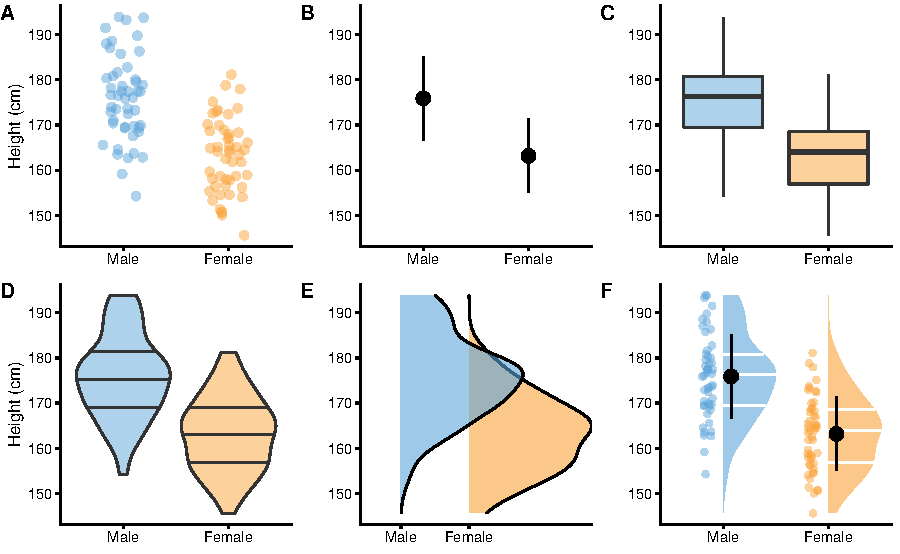
\includegraphics[width=0.9\linewidth]{02-Description_files/figure-latex/common-techniques-to-visualize-independent-groups-1} 

}

\caption{\textbf{Common techniques to visualize independent groups observations}. Before any analysis takes place, it is always a good practice to visualize the data first. Ideally, we want to visualize the complete data set, rather than only provide descriptive summaries, such as means. \textbf{A.} Simple scatter-plot with jitter to avoid overlap between the points. \textbf{B.} Mean and standard deviation as error bars. \textbf{C.} Box-plot. Horizontal line represents median, or 50th percentile, whereas boxes represent 25th and 75th percentile. Vertical lines usually represent min and max, although they can extend up to 1.5xIQR (inter-quartile range) with point outside of that interval plotted as \emph{outliers}. \textbf{D.} Violin plots representing double-side density plots with 25th, 50th and 75th percentile lines. \textbf{E.} Density plots indicating sample distribution. \textbf{F.} Raincloud plot (Allen et al. \protect\hyperlink{ref-allenRaincloudPlotsMultiplatform2019}{2019}, \protect\hyperlink{ref-allenRaincloudplotsTutorialsCodebase2018}{2018}) which combine kernel density plots as \emph{clouds} with accompanying 25th, 50th and 75th percentile lines, mean±SD error bars and jittered points as \emph{rain}}\label{fig:common-techniques-to-visualize-independent-groups}
\end{figure}



Commonly provided descriptive statistics for each group can be found in the Table \ref{tab:common-descriptive-statistics-or-estimators}. \texttt{Mean}, \texttt{median} and \texttt{mode} are common measures of central tendencies. \emph{Standard deviation} (\texttt{SD}), \emph{median absolute difference} (\texttt{MAD}), \emph{inter-quartile range} (\texttt{IQR}), \texttt{min}, \texttt{max} and \texttt{range} are common measures of spread or dispersion. \emph{Percent coefficient of variation} (\texttt{\%\ CV}) is also a measure of dispersion, but \emph{standardized}\footnote{\emph{Standardization} is the process of putting different variables on the same scale. This allows for easier comparison, as well as graphing using a common axis. For example, variables are usually standardized by using Z-Score (\(z_{i} = \frac{x_{i} - \overline{x}}{SD_{x}}\)) which has a mean of zero and a standard deviation of 1.} which allows comparison of variables that are on different scales. \emph{Skewness} (\texttt{skew}) is usually described as a measure of a symmetry. A perfectly symmetrical data set will have a skewness of 0. \texttt{Kurtosis} measures the tail-heaviness of the distribution. More in depth discussion of descriptive estimators, particularly \emph{robust estimators} (Rousselet, Pernet, and Wilcox \protect\hyperlink{ref-rousseletDifferencesMeansRobust2017}{2017}; Wilcox, Peterson, and McNitt-Gray \protect\hyperlink{ref-wilcoxDataAnalysesWhen2018}{2018}; Wilcox and Rousselet \protect\hyperlink{ref-wilcoxGuideRobustStatistical2017}{2017}; Wilcox \protect\hyperlink{ref-wilcoxIntroductionRobustEstimation2016}{2016}) is beyond the topic of this short overview.



\begin{table}

\caption{\label{tab:common-descriptive-statistics-or-estimators}\textbf{Common descriptive statistics or estimators}}
\centering
\begin{tabular}[t]{lrr}
\toprule
Estimator & Male & Female\\
\midrule
n & 50.00 & 50.00\\
mean (cm) & 175.90 & 163.18\\
SD (cm) & 9.32 & 8.20\\
\% CV & 5.30 & 5.02\\
median (cm) & 176.30 & 164.00\\
\addlinespace
MAD (cm) & 9.52 & 8.86\\
IQR (cm) & 11.24 & 11.67\\
mode (cm) & 176.26 & 164.94\\
min (cm) & 154.24 & 145.59\\
max (cm) & 193.90 & 181.12\\
\addlinespace
range (cm) & 39.66 & 35.53\\
skew & 0.08 & 0.08\\
kurtosis & -0.53 & -0.69\\
\bottomrule
\end{tabular}
\end{table}

\hypertarget{sample-mean-as-the-simplest-statistical-model}{%
\subsection{\texorpdfstring{Sample \texttt{mean} as the simplest statistical model}{Sample mean as the simplest statistical model}}\label{sample-mean-as-the-simplest-statistical-model}}

In the \protect\hyperlink{introduction}{Introduction} of this book, statistical models are defined as ``Small Worlds'' or simplifications of the complex and uncertain reality. From this perspective, sample \texttt{mean} can be considered the simplest statistical model. With this estimator we are representing all of the data points with one quantitative summary (i.e.~\emph{aggregate}). However, how do we choose an estimate that represents the sample the best? Estimate that has the minimal \emph{error} is selected as the \emph{optimal} representative. Error is defined using a \emph{loss function} that penalizes difference between the model estimate or prediction (\(\hat{y_i}\)) and observations (\(y_i\)) (Equation \eqref{eq:loss-function}). The difference between model prediction (\(\hat{y_i}\)) and observations (\(y_i\)) is called \emph{residual}.

\begin{equation}
  Loss \: function = f(observed, predicted)
  \label{eq:loss-function}
\end{equation}

Two most common loss functions are \emph{absolute loss} (also referred to as \(L1\)) (Equation \eqref{eq:absolute-loss}) and \emph{quadratic loss} (also referred to as \emph{squared errors} or \(L2\)) (Equation \eqref{eq:quadratic-loss}). Please refer to section \protect\hyperlink{sample-mean-as-the-simplest-predictive-model}{Sample \texttt{mean} as the simplest predictive model} in \protect\hyperlink{prediction}{Prediction} chapter for more examples.

\begin{equation}
  absolute \: loss = \mid{\hat{y_i} - y_i\mid}
  \label{eq:absolute-loss}
\end{equation}

\begin{equation}
  quadratic \: loss = (\hat{y_i} - y_i)^2
  \label{eq:quadratic-loss}
\end{equation}

\emph{Cost function} is an \emph{aggregate} of the loss function (Equation \eqref{eq:cost-function}).

\begin{equation}
  Cost \: function = f(Loss \: function (observed, predicted))
  \label{eq:cost-function}
\end{equation}

Since loss function is defined on a data point (i.e.~\(y_i\)), we need to aggregate losses into a single metric. This is done with a cost function, usually using \texttt{sum} or \texttt{mean}.

One such cost function is \emph{root-mean-square-error} (\texttt{RMSE}) (Equation \eqref{eq:rmse-equation}). \texttt{RMSE} takes the square root of the mean of the quadratic loss (note the \((\hat{y_i} - y_i)^2\) in the \texttt{RMSE} equation, which represent quadratic loss). \texttt{RMSE} thus represents a measure of the \emph{model fit}, or how good the model fits the data. Lower \texttt{RMSE} means lower error and thus a better fit.

\begin{equation}
  RMSE = \sqrt{\frac{1}{n}\Sigma_{i=1}^{n}(\hat{y_i} - y_i)^2}
  \label{eq:rmse-equation}
\end{equation}

By using body height data from the female group, we can \emph{search} for a body height estimate that minimizes the \texttt{RMSE} (Figure \ref{fig:sample-mean-as-the-simplest-statistical-model}). That body height estimate would be considered the best representative of the sample, and thus the simplest statistical model.

\begin{figure}[!htb]

{\centering 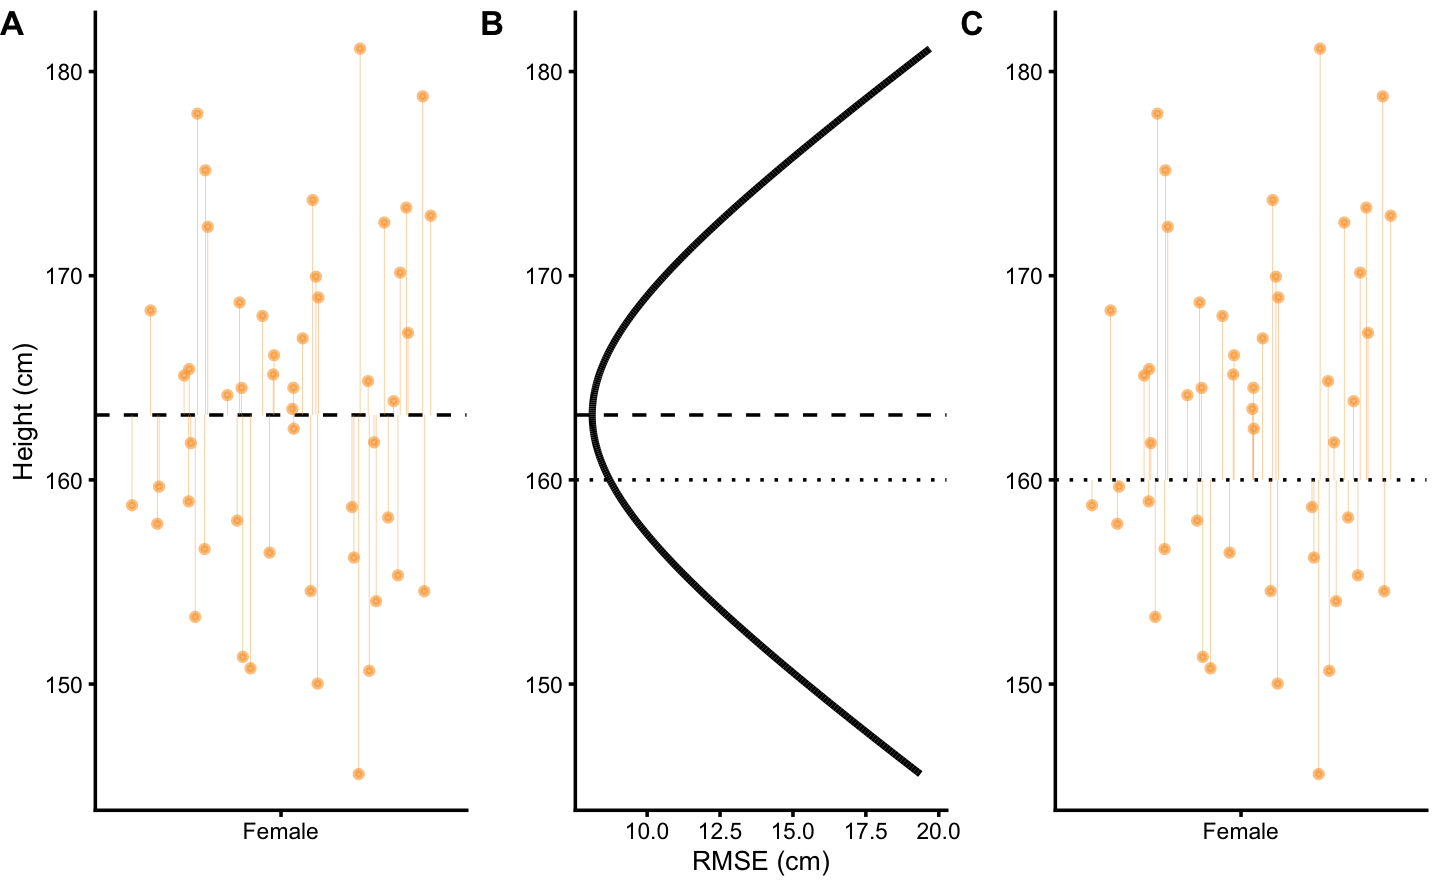
\includegraphics[width=0.9\linewidth]{02-Description_files/figure-latex/sample-mean-as-the-simplest-statistical-model-1} 

}

\caption{\textbf{Sample mean as the simplest statistical model.} \textbf{A.} Dashed line represents the estimate, in this case the \texttt{mean} of the sample. Vertical line represent residuals between estimate and observed values. \textbf{B.} Each estimate has a \texttt{RMSE} value. Central tendency estimate with the lowest \texttt{RMSE} value is the sample \texttt{mean}. \textbf{C.} Similar to panel A, this panel depicts residuals for a central tendency estimate with higher \texttt{RMSE}}\label{fig:sample-mean-as-the-simplest-statistical-model}
\end{figure}



As the result of this search, the body height estimate that minimizes the error is 163.18cm, and accompanying RMSE is equal to 8.12cm. As it can be read from the Table \ref{tab:common-descriptive-statistics-or-estimators}, this optimal body height estimate is equal to calculated sample \texttt{mean}. Standard deviation of the sample is equal to \texttt{RMSE}\footnote{As can be noticed, \texttt{RMSE} and \texttt{SD} are not exactly the same. This is because a sample \texttt{SD} equation uses \(n-1\) instead of \(n\): \(SD = \sqrt{\frac{1}{n-1}\Sigma_{i=1}^{n}(y_i -\bar{y})^2}\), where \(\bar{y}\) represents the \texttt{mean}. Remember that \(\hat{y_i}\) represents the model estimate. In this case model estimate \(\hat{y_i}\) and sample \texttt{mean} \(\bar{y}\) are the same. Sample \texttt{SD} uses \(n-1\) since this represents \emph{unbiased} estimator of the \emph{population} \texttt{SD}. More about this topic will be covered in \protect\hyperlink{statistical-inference}{Statistical inference} section.}. From statistical modeling perspective, sample mean can be considered sample estimate that minimizes the sample \texttt{SD}, and sample \texttt{SD} can be seen as the measure of the model fit.

This search for the optimal estimate that minimizes the cost function can be expanded to other statistical models. For example, linear regression can be seen as a search for the line that minimizes \texttt{RMSE}. This approach of estimating model parameters or estimators belongs to the family of \emph{ordinary least squares} (OLS) methods, although there are other approaches such as \emph{maximum likelihood estimation} (MLE) which will be discussed in \protect\hyperlink{statistical-inference}{Statistical inference} section (Foreman \protect\hyperlink{ref-foremanDataSmartUsing2014}{2014}). The solutions to some of these models can be found \emph{analytically}\footnote{The analytic solution for the central tendency estimate that minimizes \texttt{SD} is, of course, the sample \texttt{mean} (\(\frac{1}{n}\Sigma_{i=1}^{n}y_i\)).}, but for some there is no analytic solution and \emph{computational} approaches must be utilized. These computation approaches are referred to as \emph{optimization algorithms}. The example given here involves only one parameter that needs to be optimized, in this case body height estimate, but real-life problems involve numerous parameters. The simple search through parameters \emph{state-space} would take forever when it comes to problems involving more than only a few parameters. Algorithms that solve this computational problems are numerous, out of which the most popular ones are \emph{gradient descent}, and \emph{Markov Chain Monte-Carlo} (MCMC), which is utilized in \emph{Bayesian inference} (will be discussed in \protect\hyperlink{bayesian-perspective}{Bayesian perspective} section).

The take-home message from this short interlude is that even the simple descriptive statistics can be seen as statistical models.

If we take another cost function, for example \emph{mean absolute error} (\texttt{MAE}) (Equation \eqref{eq:mae-equation}) and if we \emph{optimize} so that the sample central tendency estimate minimizes MAE, we will get \texttt{median} estimator.

\begin{equation}
  MAE = \frac{1}{n}\Sigma_{i=1}^{n}\mid{\hat{y_i} - y_i\mid}
  \label{eq:mae-equation}
\end{equation}

We will expand this discussion about loss functions, cost functions, and performance metrics in \protect\hyperlink{sample-mean-as-the-simplest-predictive-model}{Sample \texttt{mean} as the simplest predictive model} section. For more information please check the package \emph{Metrics} (Hamner and Frasco \protect\hyperlink{ref-R-Metrics}{2018}) and the following references (Botchkarev \protect\hyperlink{ref-botchkarevNewTypologyDesign2019}{2019}; Chai and Draxler \protect\hyperlink{ref-chaiRootMeanSquare2014}{2014}; Willmott and Matsuura \protect\hyperlink{ref-willmottAdvantagesMeanAbsolute2005}{2005}; Barron \protect\hyperlink{ref-barronGeneralAdaptiveRobust2019}{2019}).

\hypertarget{effect-sizes}{%
\subsection{Effect Sizes}\label{effect-sizes}}

Besides describing groups, we are often interested in comparing them. In order to achieve this task, a collection of estimators termed \emph{effect size statistics} are utilized. Effect size can be defined in a \emph{narrow sense} or in a \emph{broad sense}. Briefly, the narrow sense refers to a family of standardized measures such as \texttt{Cohen’s\ d}, while the broad sense refers to any measure of interest, standardized or not. The approach to effect size statistics in this book is thus in a broad sense of the definition, in which all group comparison estimators are considered effect sizes statistics. In order to estimate effect sizes, one group needs to be considered \emph{baseline} or \emph{control}. The most common effect size statistics can be found in the Table \ref{tab:effect-size-statistics-for-estimating-differences-between-two-independent-groups} where female body height is considered baseline and compared with male body height.



\begin{table}

\caption{\label{tab:effect-size-statistics-for-estimating-differences-between-two-independent-groups}\textbf{Effect size statistics for estimating differences between two independent groups}}
\centering
\resizebox{\linewidth}{!}{
\begin{tabular}[t]{rrrrrrrr}
\toprule
Difference (cm) & SDdiff (cm) & \% CVdiff & \% Difference & Ratio & Cohen's d & CLES & OVL\\
\midrule
12.73 & 12.41 & 97.55 & 7.8 & 1.08 & 1.45 & 0.85 & 0.47\\
\bottomrule
\end{tabular}}
\end{table}

\texttt{Difference}, or \texttt{mean\ difference} (\texttt{mean\ diff}) is calculated by subtracting group \texttt{means}. Using body height as an example, the \texttt{mean\ diff} between males and females is calculated by using the following equation \eqref{eq:mean-difference-equation}:

\begin{equation}
  \begin{split}
    mean_{difference} &= mean_{males} - mean_{females} \\
    mean_{males} &= \frac{1}{n}\Sigma_{i=1}^{n}male_i  \\
    mean_{females} &= \frac{1}{n}\Sigma_{i=1}^{n}female_i
  \end{split}
  \label{eq:mean-difference-equation}
\end{equation}

\texttt{\%\ CVdiff}, or percent coefficient of variation of the difference is the standard deviation of the difference (\texttt{SDdiff} - explained shortly) divided by \texttt{mean\ diff} (Equation \eqref{eq:diff-percent-cv-equation}):

\begin{equation}
  \%\;CV_{difference} = 100\times\frac{SD_{difference}}{mean_{difference}}
  \label{eq:diff-percent-cv-equation}
\end{equation}

\texttt{\%\ Difference}, or \texttt{mean\ percent\ difference} is calculated by dividing \texttt{mean\ diff} with the \texttt{mean} of the baseline group, in this case the female group, multiplied by 100 (Equation \eqref{eq:percent-diff-equation}):

\begin{equation}
  mean_{\% difference} = 100\times\frac{mean_{difference}}{mean_{females}}
  \label{eq:percent-diff-equation}
\end{equation}

\texttt{Mean\ ratio}, as its name suggests, is simple ratio between the two \texttt{means} (Equation \eqref{eq:mean-ratio-equation}):

\begin{equation}
  mean_{ratio} = \frac{mean_{males}}{mean_{females}}
  \label{eq:mean-ratio-equation}
\end{equation}

\texttt{Cohen\textquotesingle{}s\ d} represent standardized effects size and thus preferable effect size statistic. For this reason, \texttt{Cohen\textquotesingle{}s\ d} is commonly written as ES, short of effect size. \texttt{Cohen\textquotesingle{}s\ d} for the independent groups is calculated by dividing \texttt{mean\ diff} (Equation \eqref{eq:mean-difference-equation}) with \texttt{pooled\ standard\ deviation} (\eqref{eq:cohen-diff-equation}).

\begin{equation}
  Cohen's\;d = \frac{mean_{difference}}{SD_{pooled}}
  \label{eq:cohen-diff-equation}
\end{equation}

\texttt{Pooled\ standard\ deviation} represents \emph{combined} standard deviations from two groups (Equation \eqref{eq:pooled-SD-equation}).

\begin{equation}
  SD_{pooled} = \sqrt{\frac{(n_{males} - 1) SD_{males}^2 + (n_{females} - 1) SD_{females}^2}{n_{males}+n_{females} - 2}}
  \label{eq:pooled-SD-equation}
\end{equation}

Why \texttt{Cohen\textquotesingle{}s\ d} should be used instead of other effect size estimators can be demonstrated by a simple example, coming from a study by Buchheit and Rabbani (\protect\hyperlink{ref-buchheit3015Intermittent2014}{2014}). In this study, authors examined the relationship between the performance in the \emph{YoYo Intermittent Recovery Test Level 1} (YoYoIR1) and the \emph{30-15 Intermittent Fitness Test} (30-15IFT), and compared the \emph{sensitivity} of both tests to the training. Although this study used two dependent groups (Pre-training and Post-training), the rationale can be applied to the topic of estimating effect sizes between the two independent groups. Table \ref{tab:perc-change-vs-cohensd} contains Pre-training results and the effect sizes estimated with \texttt{percent\ change}\footnote{\texttt{Percent\ change} is the same estimator as \texttt{percent\ difference}, but applied to difference between the two dependent groups (see section \protect\hyperlink{comparing-dependent-groups}{Comparing dependent groups}).} and \texttt{Cohen\textquotesingle{}s\ d}.



\begin{table}

\caption{\label{tab:perc-change-vs-cohensd}\textbf{Training intervention effect sizes for YoYoIR1 and 30-15IFT.} Modified from Buchheit and Rabbani (\protect\hyperlink{ref-buchheit3015Intermittent2014}{2014})}
\centering
\begin{tabular}[t]{lllr}
\toprule
Test & Pre-training & \% Change & Cohen's d\\
\midrule
YoYoIR1 & 1031 ± 257 m & 35 \% & 1.2\\
30-15IFT & 17.4 ± 1.1 kmh/h & 7 \% & 1.1\\
\bottomrule
\end{tabular}
\end{table}

Since YoYoIR1 and 30-15IFT utilize different scales (total meters covered and velocity reached respectively), \texttt{percent\ change} estimator is not a good choice to compare the effect sizes between the two tests\footnote{However, let's admit that we would rather report estimators of higher value, particularly if we are biased toward a specific test. ``Athletes improved on average for 35\%'' sounds much more appealing than 7\%, even if the effects estimated using \texttt{Cohen\textquotesingle{}s\ d} are the same.}. Since \texttt{Cohen\textquotesingle{}s\ d} is standardized estimator, it should be used when comparing tests or measures that are at different scales.

After estimating effect sizes, the question that naturally follows up is the question of \emph{magnitude}. In other words - ``how big is the effect?''. Since \texttt{Cohen\textquotesingle{}s\ d} is standardized estimator, it allows for establishment of qualitative magnitude thresholds. Based on the original work by Cohen (Cohen \protect\hyperlink{ref-cohenStatisticalPowerAnalysis1988}{1988}), Hopkins (Hopkins \protect\hyperlink{ref-hopkinsNewViewStatistics2006}{2006}; Hopkins et al. \protect\hyperlink{ref-hopkinsProgressiveStatisticsStudies2009}{2009}) suggested the following magnitudes of effect (Table (\ref{tab:magnitudes-of-effect}). According to the Table (\ref{tab:magnitudes-of-effect}, the body height difference between males and females would be considered \emph{large}, as well as changes in both YoYoIR1 and 30-15IFT.



\begin{table}

\caption{\label{tab:magnitudes-of-effect}\textbf{Magnitudes of effect}}
\centering
\resizebox{\linewidth}{!}{
\begin{tabular}[t]{lllllll}
\toprule
Magnitude of effect & Trivial & Small & Moderate & Large & Very Large & Nearly Perfect\\
\midrule
Cohen's d & 0 - 0.2 & 0.2 - 0.6 & 0.6 - 1.2 & 1.2 - 2.0 & 2.0 - 4.0 & > 4.0\\
\bottomrule
\end{tabular}}
\end{table}

\texttt{Cohen\textquotesingle{}s\ d}, as well as associated magnitudes of effect, are commonly hard to interpret by non-statistically trained professionals (e.g.~coaches). McGraw and Wong (\protect\hyperlink{ref-mcgrawCommonLanguageEffect1992}{1992}) suggested \emph{common language effect size} (\texttt{CLES}) estimator instead, which could be more intuitive to understand. \texttt{CLES} represents the probability that an observation sampled at random from one group will be greater than an observation sampled at random from other group. For example, if we take random male and random female from our two groups and repeat that 100 times\footnote{In other words, we are drawing 100 paired samples from the two independent groups. This makes the drawn 100 observations paired or dependent.}, how many times a male would be taller than a female (Figure \ref{fig:drawing-random-hundred-pairs})?

\begin{figure}[!htb]

{\centering 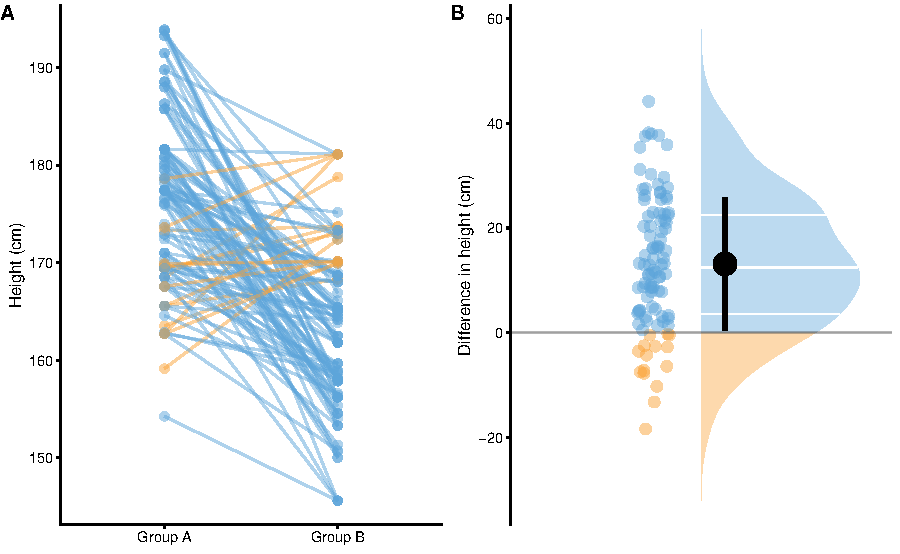
\includegraphics[width=0.9\linewidth]{02-Description_files/figure-latex/drawing-random-hundred-pairs-1} 

}

\caption{\textbf{Drawing random 100 pairs to estimate probability of males being taller than females.} \textbf{A.} Scatterplot of 100 pairs drawn at random from two samples. Since we are comparing paired males and females, lines can be drawn between each of 100 draws. Blue line indicates taller male, while orange line indicates taller female. \textbf{B.} Distribution of the difference between males and females for each of 100 pairs drawn}\label{fig:drawing-random-hundred-pairs}
\end{figure}



By using simple counting from 100 random paired samples, males are taller in 85 cases, or 85\%. By using probability, that is equal to 0.85. In other words, if I blindfoldedly, randomly select a male and a female from the two groups and if I bet that the male is taller, I would be correct 85\% of the time.

\texttt{CLES} can be estimated using \emph{brute-force} computational method, or \emph{algebraic} method. Brute-force method involves generating all possible pair-wise combinations from two groups, and in our example that is equal to \(50 \times 50 = 2500\) cases, and then simply counting in how many cases males are taller than females. This method can become very computationally intensive for groups with large sample number. Algebraic method, on the other hand, assumes normal distribution of the observations in the groups, and estimates \emph{standard deviation of the difference} (\texttt{SDdiff}) (Equation \eqref{eq:sd-diff}). Note that standard deviation of the all pairwise differences estimated with brute-force method would be very similar to algebraically derived \texttt{SDdiff}.

\begin{equation}
  SD_{difference} = \sqrt{SD_{males}^{2} + SD_{females}^{2}}
  \label{eq:sd-diff}
\end{equation}

Algebraically, \texttt{CLES} is then derived assuming normal distribution (where mean of the distribution is equal to \texttt{mean\ diff} between the groups, and standard deviation of the distribution is equal to \texttt{SDdiff}) by calculating probability of the difference scores higher than zero (see Figure \ref{fig:drawing-random-hundred-pairs}B for a visual representation). Table \ref{tab:effect-size-statistics-for-estimating-differences-between-two-independent-groups} contains algebraically computed CLES estimate.

\texttt{CLES} equivalent is utilized as a performance metric in class prediction tasks, termed \emph{area under curve} (\texttt{AUC}), where 0.5 is a predictive performance equal to a random guess, and 1 is perfect predictive separation between the two classes (James et al. \protect\hyperlink{ref-jamesIntroductionStatisticalLearning2017}{2017}; Kuhn and Johnson \protect\hyperlink{ref-kuhnAppliedPredictiveModeling2018}{2018}).

\emph{Overlap} (\texttt{OVL}) estimator represents the overlap between the two sample distributions. Providing that samples are identical, the \texttt{OVL} is equal to 1. Providing there is complete separation between the two samples, then \texttt{OVL} is equal to 0 (Figure \ref{fig:Cohen-CLES-OVL}A). \texttt{OVL} can be estimated with brute-force computational methods (which doesn't make assumptions regarding sample distribution) and with algebraic methods that make normality assumptions.

Since \texttt{Cohen\textquotesingle{}s\ d}, \texttt{CLES} and \texttt{OVL} are mathematically related, it is possible to convert one to another (assuming normal distribution of the samples and equal \texttt{SD} between the two groups for the \texttt{OVL} estimation). Figure \ref{fig:Cohen-CLES-OVL}B depicts relationship between the \texttt{Cohen\textquotesingle{}s\ d}, \texttt{CLES}, and \texttt{OVL}. Figure \ref{fig:Cohen-CLES-OVL}C depicts relationship between the \texttt{CLES} and \texttt{OVL}.

\begin{figure}[!htb]

{\centering 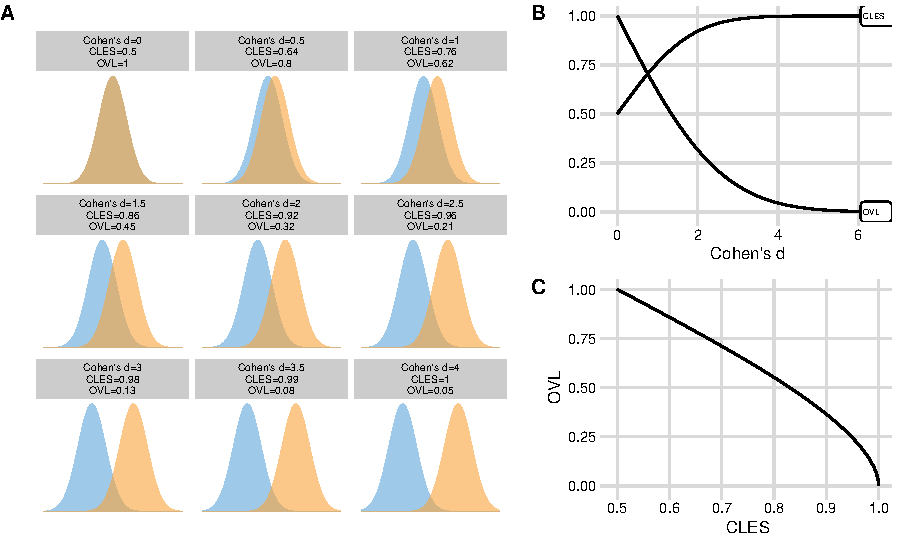
\includegraphics[width=0.9\linewidth]{02-Description_files/figure-latex/Cohen-CLES-OVL-1} 

}

\caption{\textbf{Relationship between the \texttt{Cohen\textquotesingle{}s\ d}, \texttt{CLES}, and \texttt{OVL}.} \textbf{A.} Visual display of the samples of varying degrees of separations, and calculated \texttt{Cohen\textquotesingle{}s\ d}, \texttt{CLES}, and \texttt{OVL}. \textbf{B.} Relationship between the \texttt{CLES} and \texttt{OVL} to the \texttt{Cohen\textquotesingle{}s\ d}. \textbf{C.} Relationship between the \texttt{CLES} and \texttt{OVL}}\label{fig:Cohen-CLES-OVL}
\end{figure}



Table \ref{tab:magnitudes-of-effect-CLES-OVL} contains \texttt{Cohen\textquotesingle{}s\ d} magnitudes of effect with accompanying estimated \texttt{CLES} and \texttt{OVL} thresholds.



\begin{table}

\caption{\label{tab:magnitudes-of-effect-CLES-OVL}\textbf{Magnitudes of effect for \texttt{CLES} and \texttt{OVL} estimated using \texttt{Cohen\textquotesingle{}s\ d}}}
\centering
\resizebox{\linewidth}{!}{
\begin{tabular}[t]{lllllll}
\toprule
Magnitude of effect & Trivial & Small & Moderate & Large & Very Large & Nearly Perfect\\
\midrule
Cohen's d & 0 - 0.2 & 0.2 - 0.6 & 0.6 - 1.2 & 1.2 - 2.0 & 2.0 - 4.0 & > 4.0\\
CLES & 0.50 - 0.56 & 0.56 - 0.66 & 0.66 - 0.80 & 0.80 - 0.92 & 0.92 - 1.00 & 1.00\\
OVL & 1.00 - 0.92 & 0.92 - 0.76 & 0.76 - 0.55 & 0.55 - 0.32 & 0.32 - 0.05 & 0.00\\
\bottomrule
\end{tabular}}
\end{table}

\hypertarget{the-smallest-effect-size-of-interest}{%
\subsection{The Smallest Effect Size Of Interest}\label{the-smallest-effect-size-of-interest}}

According to Cohen (\protect\hyperlink{ref-cohenStatisticalPowerAnalysis1988}{1988}), the qualitative magnitude thresholds from Table \ref{tab:magnitudes-of-effect-CLES-OVL} are ``arbitrary conventions, recommended for use only when no better basis for estimating the effect size is available'' (p.~12). But what if practitioners \emph{a priori} know what is the \emph{minimal important} effect size and are interested in judging the \emph{practical} or \emph{clinical significance} (Sainani \protect\hyperlink{ref-sainaniClinicalStatisticalSignificance2012}{2012}) of the results (in this case difference between the groups)? In other words, the \emph{smallest effect size of interest} (SESOI)\footnote{Other term for SESOI that is commonly used is \emph{region of practical equivalence} (ROPE) (Kruschke and Liddell \protect\hyperlink{ref-kruschkeBayesianDataAnalysis2018}{2018}\protect\hyperlink{ref-kruschkeBayesianDataAnalysis2018}{a}, \protect\hyperlink{ref-kruschkeBayesianNewStatistics2018}{2018}\protect\hyperlink{ref-kruschkeBayesianNewStatistics2018}{b}).}.

There is no single way to approach definition and estimation of SESOI, but it usually tends to be based on either the known \emph{measurement error} (ME) (e.g.~the minimum \emph{detectable} effect size), or the effect size that is large enough to be practically meaningful (e.g.~the minimal \emph{important} difference, or the smallest worthwhile change) (Anvari and Lakens \protect\hyperlink{ref-anvariUsingAnchorBasedMethods2019}{2019}; Will G Hopkins \protect\hyperlink{ref-hopkinsHowInterpretChanges2004}{2004}\protect\hyperlink{ref-hopkinsHowInterpretChanges2004}{a}; Will G. Hopkins \protect\hyperlink{ref-hopkinsIndividualResponsesMade2015}{2015}; King \protect\hyperlink{ref-kingPointMinimalImportant2011}{2011}; Lakens, Scheel, and Isager \protect\hyperlink{ref-lakensEquivalenceTestingPsychological2018}{2018}; Turner et al. \protect\hyperlink{ref-turnerDataAnalysisStrength2015}{2015}; Swinton et al. \protect\hyperlink{ref-swintonStatisticalFrameworkInterpret2018}{2018}; Caldwell and Cheuvront \protect\hyperlink{ref-caldwellBasicStatisticalConsiderations2019}{2019}). In this book, statistical models and estimators that utilize SESOI are referred to as \emph{magnitude-based}.

To introduce magnitude-based estimators, consider ±2.5cm to be body height SESOI\footnote{SESOI has two thresholds: \emph{lower} and \emph{upper}, or negative and positive. In this example these thresholds are -2.5cm and +2.5cm. This makes SESOI range equal to 5cm, which is calculated as \(SESOI_{upper} - SESOI_{lower}\). This range can also be referred to as \emph{equivalence range}.}, or the difference that would be practically significant. In other words, individuals with height difference within ±2.5cm would be considered practically equivalent (from the minimal important effect perspective), or it might be hard to detect this difference with a quick glance (from minimum detectable effect perspective).

The simplest magnitude-based statistics would be \texttt{mean\ diff} divided by SESOI (\texttt{Difference\ to\ SESOI}) (Equation \eqref{eq:diff-to-SESOI}). This estimator, similar to other standardized estimators (e.g.~\texttt{Cohen\textquotesingle{}s\ d}) allows comparison of variables at different scales, but it would also give more insight into differences from practical significance perspective.

\begin{equation}
  Difference\;to\;SESOI = \frac{mean_{difference}}{SESOI_{upper} - SESOI_{lower}}
  \label{eq:diff-to-SESOI}
\end{equation}

Second magnitude-based statistic is \texttt{SDdiff} divided by SESOI (\texttt{SDdiff\ to\ SESOI}) (Equation \eqref{eq:SD-diff-to-SESOI}). This estimator, similar to \texttt{\%\ CVdiff}, would answer how variable are the differences compared to SESOI.

\begin{equation}
  SDdiff\;to\;SESOI = \frac{SD_{difference}}{SESOI_{upper} - SESOI_{lower}}
  \label{eq:SD-diff-to-SESOI}
\end{equation}

Similarly, \texttt{CLES} estimator can become magnitude-based by utilizing SESOI. Rather than being interested in probability of a random male being taller than a random female (out of the two sample groups), we might be interested in estimating how probable are \emph{lower}, \emph{equivalent}, and \emph{higher} (or usually defined as \emph{harmful}, \emph{trivial}, and \emph{beneficial}) differences defined by SESOI. Practically equivalent (trivial) differences are differences ranging from \(SESOI_{lower}\) to \(SESOI_{upper}\), while everything over \(SESOI_{upper}\) is higher (or beneficial) difference and everything lower than \(SESOI_{lower}\) is lower (or harmful) difference.

Using brute-force computational method and drawing all pair-wise combinations from the two groups (50x50 = 2500 cases), and using ±2.5cm SESOI as a \emph{practically equivalent} difference\footnote{It is assumed here that SESOI is \emph{symmetrical} in both positive and negative directions. This makes the equivalent difference ranging from -2.5cm to +2.5cm. SESOI doesn't necessary needs to be symmetrical in both positive and negative directions.}, we can estimate probabilities of lower (\texttt{pLower}), equivalent (\texttt{pEquivalent}) and higher difference (\texttt{pHigher}) by calculating \emph{proportion} of cases within each magnitude band (Figure \ref{fig:pairwise-comparison}).

\begin{figure}[!htb]

{\centering 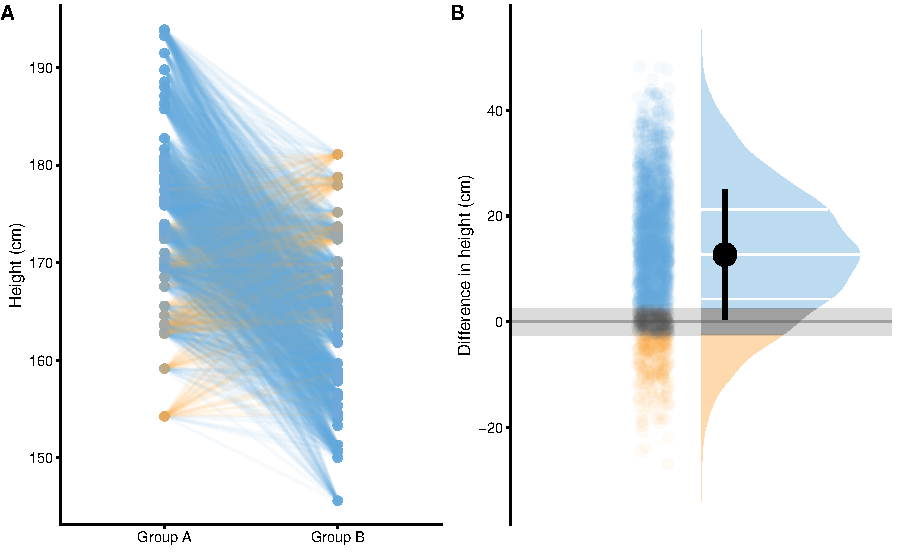
\includegraphics[width=0.9\linewidth]{02-Description_files/figure-latex/pairwise-comparison-1} 

}

\caption{\textbf{Pairwise comparison of males and females to estimate probability of lower, equivalent, and higher magnitude of difference. A.} Scatterplot of all pair-wise combinations (50x50 = 2500), drawn at random out of two samples. Since we are comparing paired males and females, lines can be drawn between each of 2500 draws. Blue line indicates males taller than females higher than SESOI, equivalent lines indicates pairs with a height difference less or equal to SESOI, while orange line indicates females taller than males higher than SESOI. \textbf{B.} Distribution of the differences between males and females for all 2500 pair-wise combinations. Grey band indicates SESOI. Surface of the distribution over SESOI (blue color) indicates probability of randomly selected male being taller than a randomly selected female (\texttt{pHigher}), with a height difference of at least SESOI magnitude. Surface of the distribution under SESOI (orange color) indicates probability of randomly selected female being taller than a randomly selected female (\texttt{pLower}), with a height difference of at least SESOI magnitude. Grey surface area indicates probability of randomly selecting male and female with a height difference within SESOI band (\texttt{pEquivalent})}\label{fig:pairwise-comparison}
\end{figure}



Table \ref{tab:table-magnitude-based-diff} contains estimated probabilities of observing lower, equivalent, and higher differences in height between the randomly selected male and female using brute-force computational method and algebraic method. These estimates answer the following question ``If I compare random male and random female from my sample, how probable are lower/equivalent/higher magnitudes of difference in height?''. Asking such a magnitude-based question regarding the random individual difference represents a form of prediction question and predictive task. In this book, such questions are answered with \emph{magnitude-based prediction} approaches.



\begin{table}

\caption{\label{tab:table-magnitude-based-diff}\textbf{Estimated probabilities of observing lower, equivalent, and higher differences in height}}
\centering
\begin{tabular}[t]{lrrr}
\toprule
Method & pLower & pEquivalent & pHigher\\
\midrule
brute-force & 0.110 & 0.096 & 0.794\\
algebraic & 0.111 & 0.095 & 0.794\\
\bottomrule
\end{tabular}
\end{table}

It is common to represent means as \emph{systematic component} or \emph{fixed effect} (e.g.~\texttt{mean\ difference}), and variability around the mean (i.e.~\texttt{SDdiff}) as \emph{stochastic component} or \emph{random effect}. It is unfortunate that the common statistical modeling and analysis, particularly in sport science, takes the stance of approaching and treating between-individual variation as \emph{random error}. The approach suggested in this book complements \emph{group-based} or \emph{average-based} statistics with magnitude-based predictions that aim to help in answering individual-based questions, common to sport practitioners. Table \ref{tab:magnitude-based-estimators-diff} contains discussed magnitude-based estimators that can complement common effect size statistics (Table \ref{tab:effect-size-statistics-for-estimating-differences-between-two-independent-groups}) when comparing two independent groups.



\begin{table}

\caption{\label{tab:magnitude-based-estimators-diff}\textbf{Magnitude-based effect size statistics for estimating difference between two independent groups}}
\centering
\resizebox{\linewidth}{!}{
\begin{tabular}[t]{rrrrrrr}
\toprule
SESOI lower (cm) & SESOI upper (cm) & Difference to SESOI & SDdiff to SESOI & pLower & pEquivalent & pHigher\\
\midrule
-2.5 & 2.5 & 2.55 & 2.48 & 0.11 & 0.09 & 0.79\\
\bottomrule
\end{tabular}}
\end{table}

\hypertarget{comparing-dependent-groups}{%
\section{Comparing dependent groups}\label{comparing-dependent-groups}}

As an example of dependent or paired groups descriptive analysis, let's consider the simple \emph{Pre-test} and \emph{Post-test} design. We have given training intervention to a group of N=20 males involving bench-press training. Training intervention involved performing bench pressing two times a week for 16 weeks. One-repetition-maximum (1RM) in the bench press was performed before (Pre-test) and after (Post-test) training intervention. Table \ref{tab:bench-press-1RM-pre-post} contains individual Pre-test and Post-test scores, as well as the Change in the bench press 1RM.



\begin{table}

\caption{\label{tab:bench-press-1RM-pre-post}\textbf{Individual Pre and Post scores, as well as Change in the bench press 1RM}}
\centering
\begin{tabular}[t]{lrrr}
\toprule
Athlete & Pre-test (kg) & Post-test (kg) & Change (kg)\\
\midrule
Athlete 01 & 111.80 & 121.42 & 9.62\\
Athlete 02 & 95.95 & 102.13 & 6.18\\
Athlete 03 & 105.87 & 125.56 & 19.69\\
Athlete 04 & 98.79 & 109.67 & 10.87\\
Athlete 05 & 95.81 & 108.11 & 12.30\\
\addlinespace
Athlete 06 & 95.27 & 92.67 & -2.60\\
Athlete 07 & 97.75 & 106.03 & 8.28\\
Athlete 08 & 106.50 & 109.51 & 3.01\\
Athlete 09 & 80.62 & 95.96 & 15.34\\
Athlete 10 & 100.40 & 94.30 & -6.11\\
\addlinespace
Athlete 11 & 82.71 & 78.91 & -3.80\\
Athlete 12 & 102.89 & 93.98 & -8.91\\
Athlete 13 & 91.34 & 105.21 & 13.87\\
Athlete 14 & 111.14 & 108.07 & -3.07\\
Athlete 15 & 95.13 & 96.01 & 0.88\\
\addlinespace
Athlete 16 & 109.12 & 112.12 & 3.00\\
Athlete 17 & 91.87 & 103.41 & 11.54\\
Athlete 18 & 92.16 & 103.93 & 11.77\\
Athlete 19 & 108.88 & 119.72 & 10.84\\
Athlete 20 & 97.94 & 95.91 & -2.03\\
\bottomrule
\end{tabular}
\end{table}

The results of this simple Pre-test and Post-test design can be described in multiple ways. Here, I will present the three most common approaches.

\hypertarget{describing-groups-as-independent}{%
\subsection{Describing groups as independent}\label{describing-groups-as-independent}}

The simplest analysis involve descriptive statistics assuming groups as independent. Table \ref{tab:bench-press-data-independent-summary} contains descriptive statistics applied to Pre-test, Post-test and Change scores as independent. Figure \ref{fig:bench-press-pre-post-raincloud} visualizes the scores using three raincloud plots.



\begin{table}

\caption{\label{tab:bench-press-data-independent-summary}\textbf{Descriptive analysis of the Pre-test, Post-test, and Change as independent samples}}
\centering
\begin{tabular}[t]{lrrr}
\toprule
Estimator & Pre-test & Post-test & Change\\
\midrule
n & 20.00 & 20.00 & 20.00\\
mean (kg) & 98.60 & 104.13 & 5.53\\
SD (kg) & 8.70 & 11.08 & 8.05\\
\% CV & 8.83 & 10.64 & 145.46\\
median (kg) & 97.84 & 104.57 & 7.23\\
\addlinespace
MAD (kg) & 8.64 & 11.94 & 8.46\\
IQR (kg) & 11.64 & 13.60 & 13.77\\
mode (kg) & 96.49 & 105.76 & 10.78\\
min (kg) & 80.62 & 78.91 & -8.91\\
max (kg) & 111.80 & 125.56 & 19.69\\
\addlinespace
range (kg) & 31.18 & 46.64 & 28.60\\
skew & -0.26 & -0.05 & -0.16\\
kurtosis & -0.73 & -0.28 & -1.28\\
\bottomrule
\end{tabular}
\end{table}

\begin{figure}[!htb]

{\centering 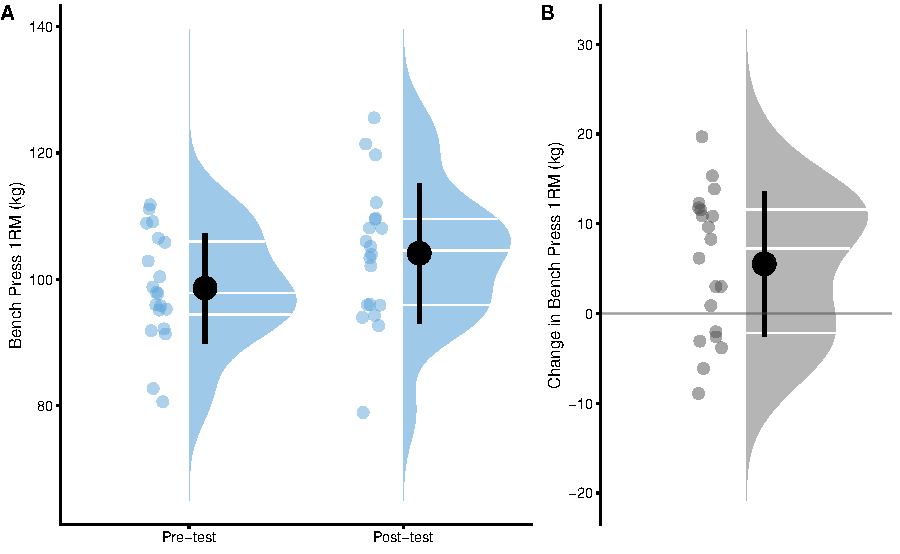
\includegraphics[width=0.9\linewidth]{02-Description_files/figure-latex/bench-press-pre-post-raincloud-1} 

}

\caption{\textbf{Raincloud plots of the Pre-test, Post-test and Change scores in the bench press 1RM. A. }Distribution of the Pre-test and Post-test scores. \textbf{B.} Distribution of the Change score}\label{fig:bench-press-pre-post-raincloud}
\end{figure}



\hypertarget{effect-sizes-1}{%
\subsection{Effect Sizes}\label{effect-sizes-1}}

Table \ref{tab:change-effect-size} contains the most common effect size estimators utilized when describing change in the Pre-Post paired design. The terminology utilized in this book differentiates between the \emph{difference} which is used in independent groups and the \emph{change} which is used in paired or dependent groups



\begin{table}

\caption{\label{tab:change-effect-size}\textbf{Effect size statistics for estimating change in two dependent groups}}
\centering
\resizebox{\linewidth}{!}{
\begin{tabular}[t]{rrrrrrrr}
\toprule
Change (kg) & SDchange (kg) & \% CVchange & \% Change & Ratio & Cohen's d & CLES & OVL\\
\midrule
5.53 & 8.05 & 145.46 & 5.75 & 1.06 & 0.64 & 0.65 & 0.75\\
\bottomrule
\end{tabular}}
\end{table}

\texttt{Change}, or \texttt{mean\ change} is calculated by taking average of the change score (Equation \eqref{eq:mean-change-equation}). Change score is simple difference between Pre-test and Post-test.

\begin{equation}
  \begin{split}
    mean_{change} &= \frac{1}{n}\Sigma_{i=1}^{n}(post_{i}-pre_{i}) \\
    mean_{change} &= \frac{1}{n}\Sigma_{i=1}^{n}change_{i} \\
    change_{i} &= post_{i}-pre_{i}
  \end{split}
  \label{eq:mean-change-equation}
\end{equation}

\texttt{SDchange}, or standard deviation of the change is a simple standard deviation of the change (Equation \eqref{eq:SD-change-equation}). It represents a measure of dispersion of the change scores.

\begin{equation}
  SD_{change} = \sqrt{\frac{1}{n-1}\Sigma_{i=1}^{n}(change_i -mean_{change})^2}
  \label{eq:SD-change-equation}
\end{equation}

\texttt{\%\ CVchange}, or percent coefficient of variation of the change is the \texttt{SDchange} divided by \texttt{mean\ change} (Equation \eqref{eq:CV-change-coeff}).

\begin{equation}
  \%\;CV_{change} = 100\times\frac{SD_{change}}{mean_{change}}
  \label{eq:CV-change-coeff}
\end{equation}

\texttt{\%\ Change}, or \texttt{Mean\ percent\ change} is calculated by taking a mean of the ratio between the change and the Pre-test, multiplied by 100 (Equation \eqref{eq:percent-change-equation}).

\begin{equation}
  mean_{\% change} = 100\times\frac{1}{n}\Sigma_{i}^{n}\frac{change_{i}}{pre_{i}}
 \label{eq:percent-change-equation}
\end{equation}

\texttt{Mean\ ratio} represents mean of the Post-test to Pre-test scores ratios (Equation \eqref{eq:mean-ratio-paired-equation}).

\begin{equation}
  mean_{ratio} = \frac{1}{n}\Sigma_{i}^{n}\frac{post_{i}}{pre_{i}}
  \label{eq:mean-ratio-paired-equation}
\end{equation}

\texttt{Cohen\textquotesingle{}s\ d} represents standardized effect size of the change. In the paired design, \texttt{Cohen\textquotesingle{}s\ d} is calculated by dividing \texttt{mean\ change} with standard deviation of the Pre-test scores (\texttt{SDpre}) (Equation \eqref{eq:cohens-d-paired}).

\begin{equation}
  Cohen's\;d = \frac{mean_{change}}{SD_{pre}}
  \label{eq:cohens-d-paired}
\end{equation}

\texttt{CLES} for the paired groups represents probability of observing positive change. \texttt{OVL}, equally to the independent groups, represents overlap between the Pre-test and Post-test scores.

Magnitude-based effect size estimators involve the use of SESOI and can be found on Table \ref{tab:change-MB-stats}. Similarly to magnitude-based effect size estimators with the independent groups, magnitude-based effect size estimators with the paired group involve \texttt{Change\ to\ SESOI}, \texttt{SDchange\ to\ SESOI} as well as proportions of lower (\texttt{pLower}), equivalent (\texttt{pEquivalent}) and higher (\texttt{pHigher}) change scores.



\begin{table}

\caption{\label{tab:change-MB-stats}\textbf{Magnitude-based effect size statistics for estimating change between two dependent groups}}
\centering
\resizebox{\linewidth}{!}{
\begin{tabular}[t]{lrrrrr}
\toprule
SESOI (kg) & Change to SESOI & SDchange to SESOI & pLower & pEquivalent & pHigher\\
\midrule
±5 & 0.55 & 0.81 & 0.1 & 0.37 & 0.53\\
\bottomrule
\end{tabular}}
\end{table}

Figure \ref{fig:bench-press-pair-change} depicts visually how proportions of lower, equivalent, and higher change scores are estimated. Same as with two independent groups, these proportions can be estimated using the brute-force method (i.e.~simple counting of the change scores withing lower, trivial, and higher zones), or algebraic where \texttt{SDchange} is utilized and assumption of the normally distributed change scores is made.

\begin{figure}[!htb]

{\centering 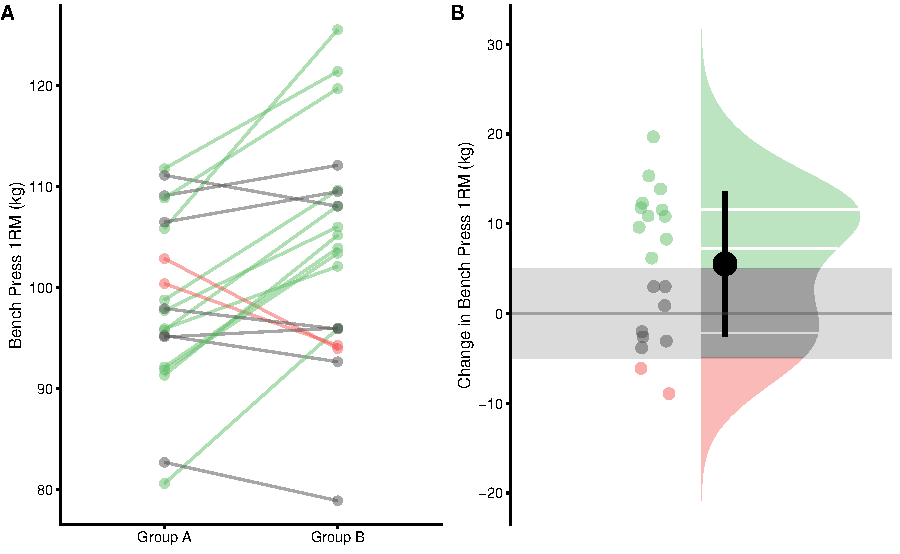
\includegraphics[width=0.9\linewidth]{02-Description_files/figure-latex/bench-press-pair-change-1} 

}

\caption{\textbf{Visual analysis of the dependent groups scores using SESOI. A. }Scatter plot of Pre-test and Post-test scores. Green line indicates change higher than SESOI upper, grey line indicates change within SESOI band, and red line indicates negative change lower than SESOI lower. \textbf{B.} Distribution of the change scores. Green area represents proportion of change scores higher than SESOI upper, red area represents proportion of negative change scores lower than SESOI lower, and grey area indicates equivalent change, which is within SESOI band}\label{fig:bench-press-pair-change}
\end{figure}



It might be tempting to claim that this intervention is \emph{causing} changes in the bench press 1RM, but we should be vary of doing that. It is important to keep in mind that the effect size estimators are used only descriptively without any causal connotation. To make causal claims, further criteria needs to be taken into account. This is discussed in more details in the \protect\hyperlink{causal-inference}{Causal inference} section of this book.

\hypertarget{describing-relationship-between-two-variables}{%
\section{Describing relationship between two variables}\label{describing-relationship-between-two-variables}}

So far, we have dealt with single variable descriptive statistics. However, we are often interested in relationship or \emph{association} between two variables. One of these variables takes the role of the \emph{dependent variable} (\emph{outcome} or \emph{target variable}) and the other of the \emph{independent variable} (or \emph{predictor variable}).

Let's assume we tested N=30 female soccer athletes by using two tests: (1) YoYoIR1 test (expressed in meters), and (2) \emph{maximum aerobic speed} (MAS) test (expressed in km/h)\footnote{Since YoYoIR1 test is performed in 2x20m shuttles, the minimal increment is equal to 40m. For the MAS test the minimal increment is 0.5km/h.}. Variables in this example represent observations in each test (Table \ref{tab:yoyo-mas-results}).



\begin{table}

\caption{\label{tab:yoyo-mas-results}\textbf{Results of YoYoIR1 and MAS tests for N=30 female soccer athletes}}
\centering
\begin{tabular}[t]{lrr}
\toprule
Athlete & YoYoIR1 (m) & MAS (km/h)\\
\midrule
Athlete 01 & 1640 & 15.5\\
Athlete 02 & 1080 & 15.0\\
Athlete 03 & 1440 & 15.0\\
Athlete 04 & 1200 & 15.0\\
Athlete 05 & 960 & 14.5\\
\addlinespace
Athlete 06 & 1120 & 15.0\\
Athlete 07 & 1000 & 14.5\\
Athlete 08 & 1440 & 15.0\\
Athlete 09 & 640 & 14.0\\
Athlete 10 & 1360 & 15.0\\
\addlinespace
Athlete 11 & 760 & 14.5\\
Athlete 12 & 1240 & 15.0\\
Athlete 13 & 1000 & 15.0\\
Athlete 14 & 1600 & 15.5\\
Athlete 15 & 1160 & 15.0\\
\addlinespace
Athlete 16 & 1520 & 15.0\\
Athlete 17 & 1000 & 14.5\\
Athlete 18 & 1000 & 14.5\\
Athlete 19 & 1480 & 15.5\\
Athlete 20 & 1280 & 15.0\\
\addlinespace
Athlete 21 & 1200 & 14.5\\
Athlete 22 & 1200 & 14.5\\
Athlete 23 & 1200 & 15.0\\
Athlete 24 & 1120 & 14.5\\
Athlete 25 & 1560 & 15.5\\
\addlinespace
Athlete 26 & 1120 & 14.5\\
Athlete 27 & 1640 & 15.5\\
Athlete 28 & 1280 & 15.0\\
Athlete 29 & 1040 & 14.5\\
Athlete 30 & 880 & 14.0\\
\bottomrule
\end{tabular}
\end{table}

Descriptive statistics for YoYoIR1 and MAS test results can be found in the Table \ref{tab:yoyo-mas-descriptive-stats}.



\begin{table}

\caption{\label{tab:yoyo-mas-descriptive-stats}\textbf{Descriptive statistics for YoYoIR1 and MAS test results}}
\centering
\begin{tabular}[t]{lrr}
\toprule
Estimator & YoYoIR1 & MAS\\
\midrule
n & 30.00 & 30.00\\
mean & 1205.33 & 14.85\\
SD & 255.96 & 0.42\\
\% CV & 21.24 & 2.82\\
median & 1200.00 & 15.00\\
\addlinespace
MAD & 296.52 & 0.74\\
IQR & 410.00 & 0.50\\
mode & 1131.68 & 15.00\\
min & 640.00 & 14.00\\
max & 1640.00 & 15.50\\
\addlinespace
range & 1000.00 & 1.50\\
skew & -0.02 & -0.11\\
kurtosis & -0.68 & -0.72\\
\bottomrule
\end{tabular}
\end{table}

Visual analysis in Figure \ref{fig:yoyo-mas-simple-scatterplot} depicts the association between these two tests using scatter plot.

\begin{figure}[!htb]

{\centering 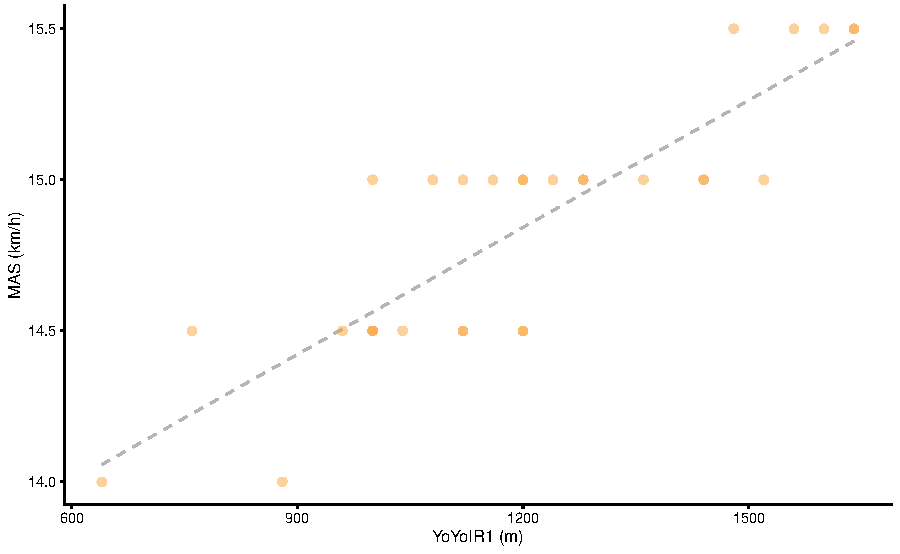
\includegraphics[width=0.9\linewidth]{02-Description_files/figure-latex/yoyo-mas-simple-scatterplot-1} 

}

\caption{\textbf{Scatter plot between two variables. }Dashed line represents linear regression line}\label{fig:yoyo-mas-simple-scatterplot}
\end{figure}



Table \ref{tab:common-estimators-association} contains common estimators of the association between two variables. All estimators except \emph{maximum information coefficient} (\texttt{MIC}) (Albanese et al. \protect\hyperlink{ref-albaneseMinervaMinepyEngine2012}{2012}\protect\hyperlink{ref-albaneseMinervaMinepyEngine2012}{b}; Reshef et al. \protect\hyperlink{ref-reshefDetectingNovelAssociations2011}{2011}) assumes linear relationship between two variables. It is thus important to visually analyze the association (see Figure \ref{fig:yoyo-mas-simple-scatterplot}) before trusting numerical estimators.



\begin{table}

\caption{\label{tab:common-estimators-association}\textbf{Common estimators of the association between two variables}}
\centering
\begin{tabular}[t]{rrr}
\toprule
Pearson r & R-squared & MIC\\
\midrule
0.86 & 0.74 & 0.55\\
\bottomrule
\end{tabular}
\end{table}

The \emph{Pearson product-moment correlation coefficient} (\texttt{Pearson\textquotesingle{}s\ r}) is a measure of the strength of the linear relationship between two variables (Equation \eqref{eq:pearson-r}).

\begin{equation}
  r = \frac{{}\sum_{i=1}^{n} (x_i - \overline{x})(y_i - \overline{y})}
  {\sqrt{\sum_{i=1}^{n} (x_i - \overline{x})^2(y_i - \overline{y})^2}}
  \label{eq:pearson-r}
\end{equation}

\texttt{Pearson\textquotesingle{}s\ r} is standardized measure that can take values ranging from -1 to +1, where 0 indicates no relationship, and -1 and +1 indicates perfect relationship. Negative \texttt{Pearson\textquotesingle{}s\ r} value represents negative association (i.e.~as one variable increases the other decreases), while positive \texttt{Pearson\textquotesingle{}s\ r} value represents positive association (i.e., as one variable increases so does the other).

\texttt{R-squared} (\(R^2\)) represents \emph{variance explained}, i.e.~how much the \emph{model} explains variance in the target variable. In this example the model is \emph{linear regression}. \texttt{R-squared} is standardized measure of association that can take values ranging from zero (no association, or no variance explained) to 1 (perfect association, or all variance explained). \texttt{R-squared}, as its name suggests, represents Pearson's r squared, but for more complex models it can be calculated using variances or \emph{mean squares} (\texttt{MS}) (Equation \eqref{eq:pearson-r}):

\begin{equation}
  \begin{split}
    R^2 &= \frac{MS_{model}}{MS_{total}} \\
    MS_{model} &= \frac{1}{n}\Sigma_{i=1}^{n}(\hat y_i - \overline y)^2 \\
    MS_{total} &= \frac{1}{n}\Sigma_{i=1}^{n}(y_i - \overline y)^2
  \end{split}
  \label{eq:r-squared}
\end{equation}

\emph{Maximal information coefficient} (\texttt{MIC}) is a novel measure of the strength of the linear or non-linear association between two variables and belongs to the \emph{maximal information-based non-parametric exploration} (MINE) class of statistics (Albanese et al. \protect\hyperlink{ref-albaneseMinervaMinepyEngine2012}{2012}\protect\hyperlink{ref-albaneseMinervaMinepyEngine2012}{b}; Reshef et al. \protect\hyperlink{ref-reshefDetectingNovelAssociations2011}{2011}). \texttt{MIC} is standardized measure of association that can take values ranging from zero (no association) to 1 (perfect association). As opposed to \texttt{Pearson\ r}, \texttt{MIC} can \emph{pick up} non-linear association between two variables.

Statistical model, or \emph{machinery} underlying \texttt{Pearson\ r} and \texttt{R-squared} is linear regression. Similar to a sample \texttt{mean} (see section \protect\hyperlink{sample-mean-as-the-simplest-statistical-model}{Sample \texttt{mean} as the simplest statistical model}), linear regression can be seen as \emph{optimization algorithm} that tries to find a line that passes through the data with the minimal error.\footnote{This approach, as already explained, belongs to the OLS approach. On the other hand, MLE tries to find a line that maximizes likelihood of the data.} A solution to this problem can be found computationally or analytically\footnote{The benefit of using \emph{squared errors} in OLS approaches, is that this \emph{optimization} (or the search for parameters that minimize \texttt{RMSE} as a cost function in this case) can be done analytically. One of the drawbacks of using squared errors (or squared residuals) is sensitivity to \emph{outliers}. Other regression approaches, such as \emph{quantiles regression} or \emph{ordinary least products} (OLP) for example, use different loss and cost functions. OLP regression will be utilized in the \protect\hyperlink{reliability}{Reliability} section of the book.}. Either way, the \emph{coefficients} (or \emph{parameters}) that need to be estimated in this example with two variables are \texttt{intercept} (\(\hat{\beta}_0\)), \texttt{slope\ \ coefficient} (\(\hat{\beta}_1\)), and \emph{residual error} (\(\hat{\epsilon}\)) (Equation \eqref{eq:linear-equation}).

\begin{equation}
  \hat{y}_i = \hat{\beta}_0 + \hat{\beta}_1 x_i + \hat{\epsilon}
  \label{eq:linear-equation}
\end{equation}

Table \ref{tab:linear-reg-estimates} contains estimates for \texttt{intercept}, \texttt{slope}, and residual error. Residual error (\(\epsilon\)) is estimated by using \emph{residual standard error} (\texttt{RSE}), which is similar to already discussed \texttt{RMSE}, but rather than dividing sum of square errors by \(n\) observations, it is divided by \(n-p\) (Equation \eqref{eq:rse-equation}). The \(p\) is the number of model parameters, in this case 2 (\texttt{intercept} and one \texttt{slope\ coefficient}).

\begin{equation}
  RSE = \sqrt{\frac{1}{n-p}\Sigma_{i=1}^{n}(y_i -\hat{y_i})^2}
  \label{eq:rse-equation}
\end{equation}



\begin{table}

\caption{\label{tab:linear-reg-estimates}Linear regression estimates for \texttt{intercept}, \texttt{slope\ coefficient}, and \texttt{RSE} when MAS is the target variable an YoYoIR1 is the predictor}
\centering
\begin{tabular}[t]{rrr}
\toprule
Intercept (km/h) & Slope & RSE (km/h)\\
\midrule
13.16 & 0.0014 & 0.22\\
\bottomrule
\end{tabular}
\end{table}

Estimated parameters in the Table \ref{tab:linear-reg-estimates} can be written using the linear equation format (Equation \eqref{eq:mas-equation}).

\begin{equation}
  MAS = 13.16 + 0.0014 \times YoYoIR1 \pm 0.22 \: km/h
  \label{eq:mas-equation}
\end{equation}

Slope coefficient of 0.0014 can be interpreted the following way: if YoYoIR1 increases by 500m, then MAS would increase by 500 x 0.0014 or 0.7km/h.

Although measures of association between two variables, such as \texttt{Pearson\textquotesingle{}s\ r} and \texttt{R-squared}, are symmetrical (meaning it doesn't matter which variable is predictor or target), one cannot reverse the linear regression equation to get YoYoIR1 from MAS as done in the Equation \eqref{eq:rse-equation}.

\begin{equation}
  \begin{split}
    MAS &= \hat{\beta}_0 + \hat{\beta}_1 \times YoYoIR1 \\
    YoYoIR1 &= \frac{-\hat{\beta}_0 + MAS}{\hat{\beta}_1} \\
    YoYoIR1 &= -\frac{\hat{\beta}_0}{\hat{\beta}_1} + \frac{1}{\hat{\beta}_1}\times MAS \\
    YoYoIR1 &= -9385.59 + 713.19 \times MAS
  \end{split}
  \label{eq:reverse-linear-equation}
\end{equation}

It can be seen that the reverse parameters from \eqref{eq:rse-equation} differ from the parameters in the Table \ref{tab:reverse-estimates-table} which are estimated using YoYoIR1 as the target variable an MAS as the predictor variable.



\begin{table}

\caption{\label{tab:reverse-estimates-table}Linear regression estimates for \texttt{intercept}, \texttt{slope\ coefficient}, and \texttt{RSE} when YoYoIR1 is the target variable an MAS is the predictor}
\centering
\begin{tabular}[t]{rrr}
\toprule
Intercept (m) & Slope & RSE (m)\\
\midrule
-6589.82 & 524.93 & 133.84\\
\bottomrule
\end{tabular}
\end{table}

This difference between reversed parameters and correctly estimated can be visually seen as non-identical linear regression lines in the Figure \ref{fig:reverse-linear}.

\begin{figure}[!htb]

{\centering 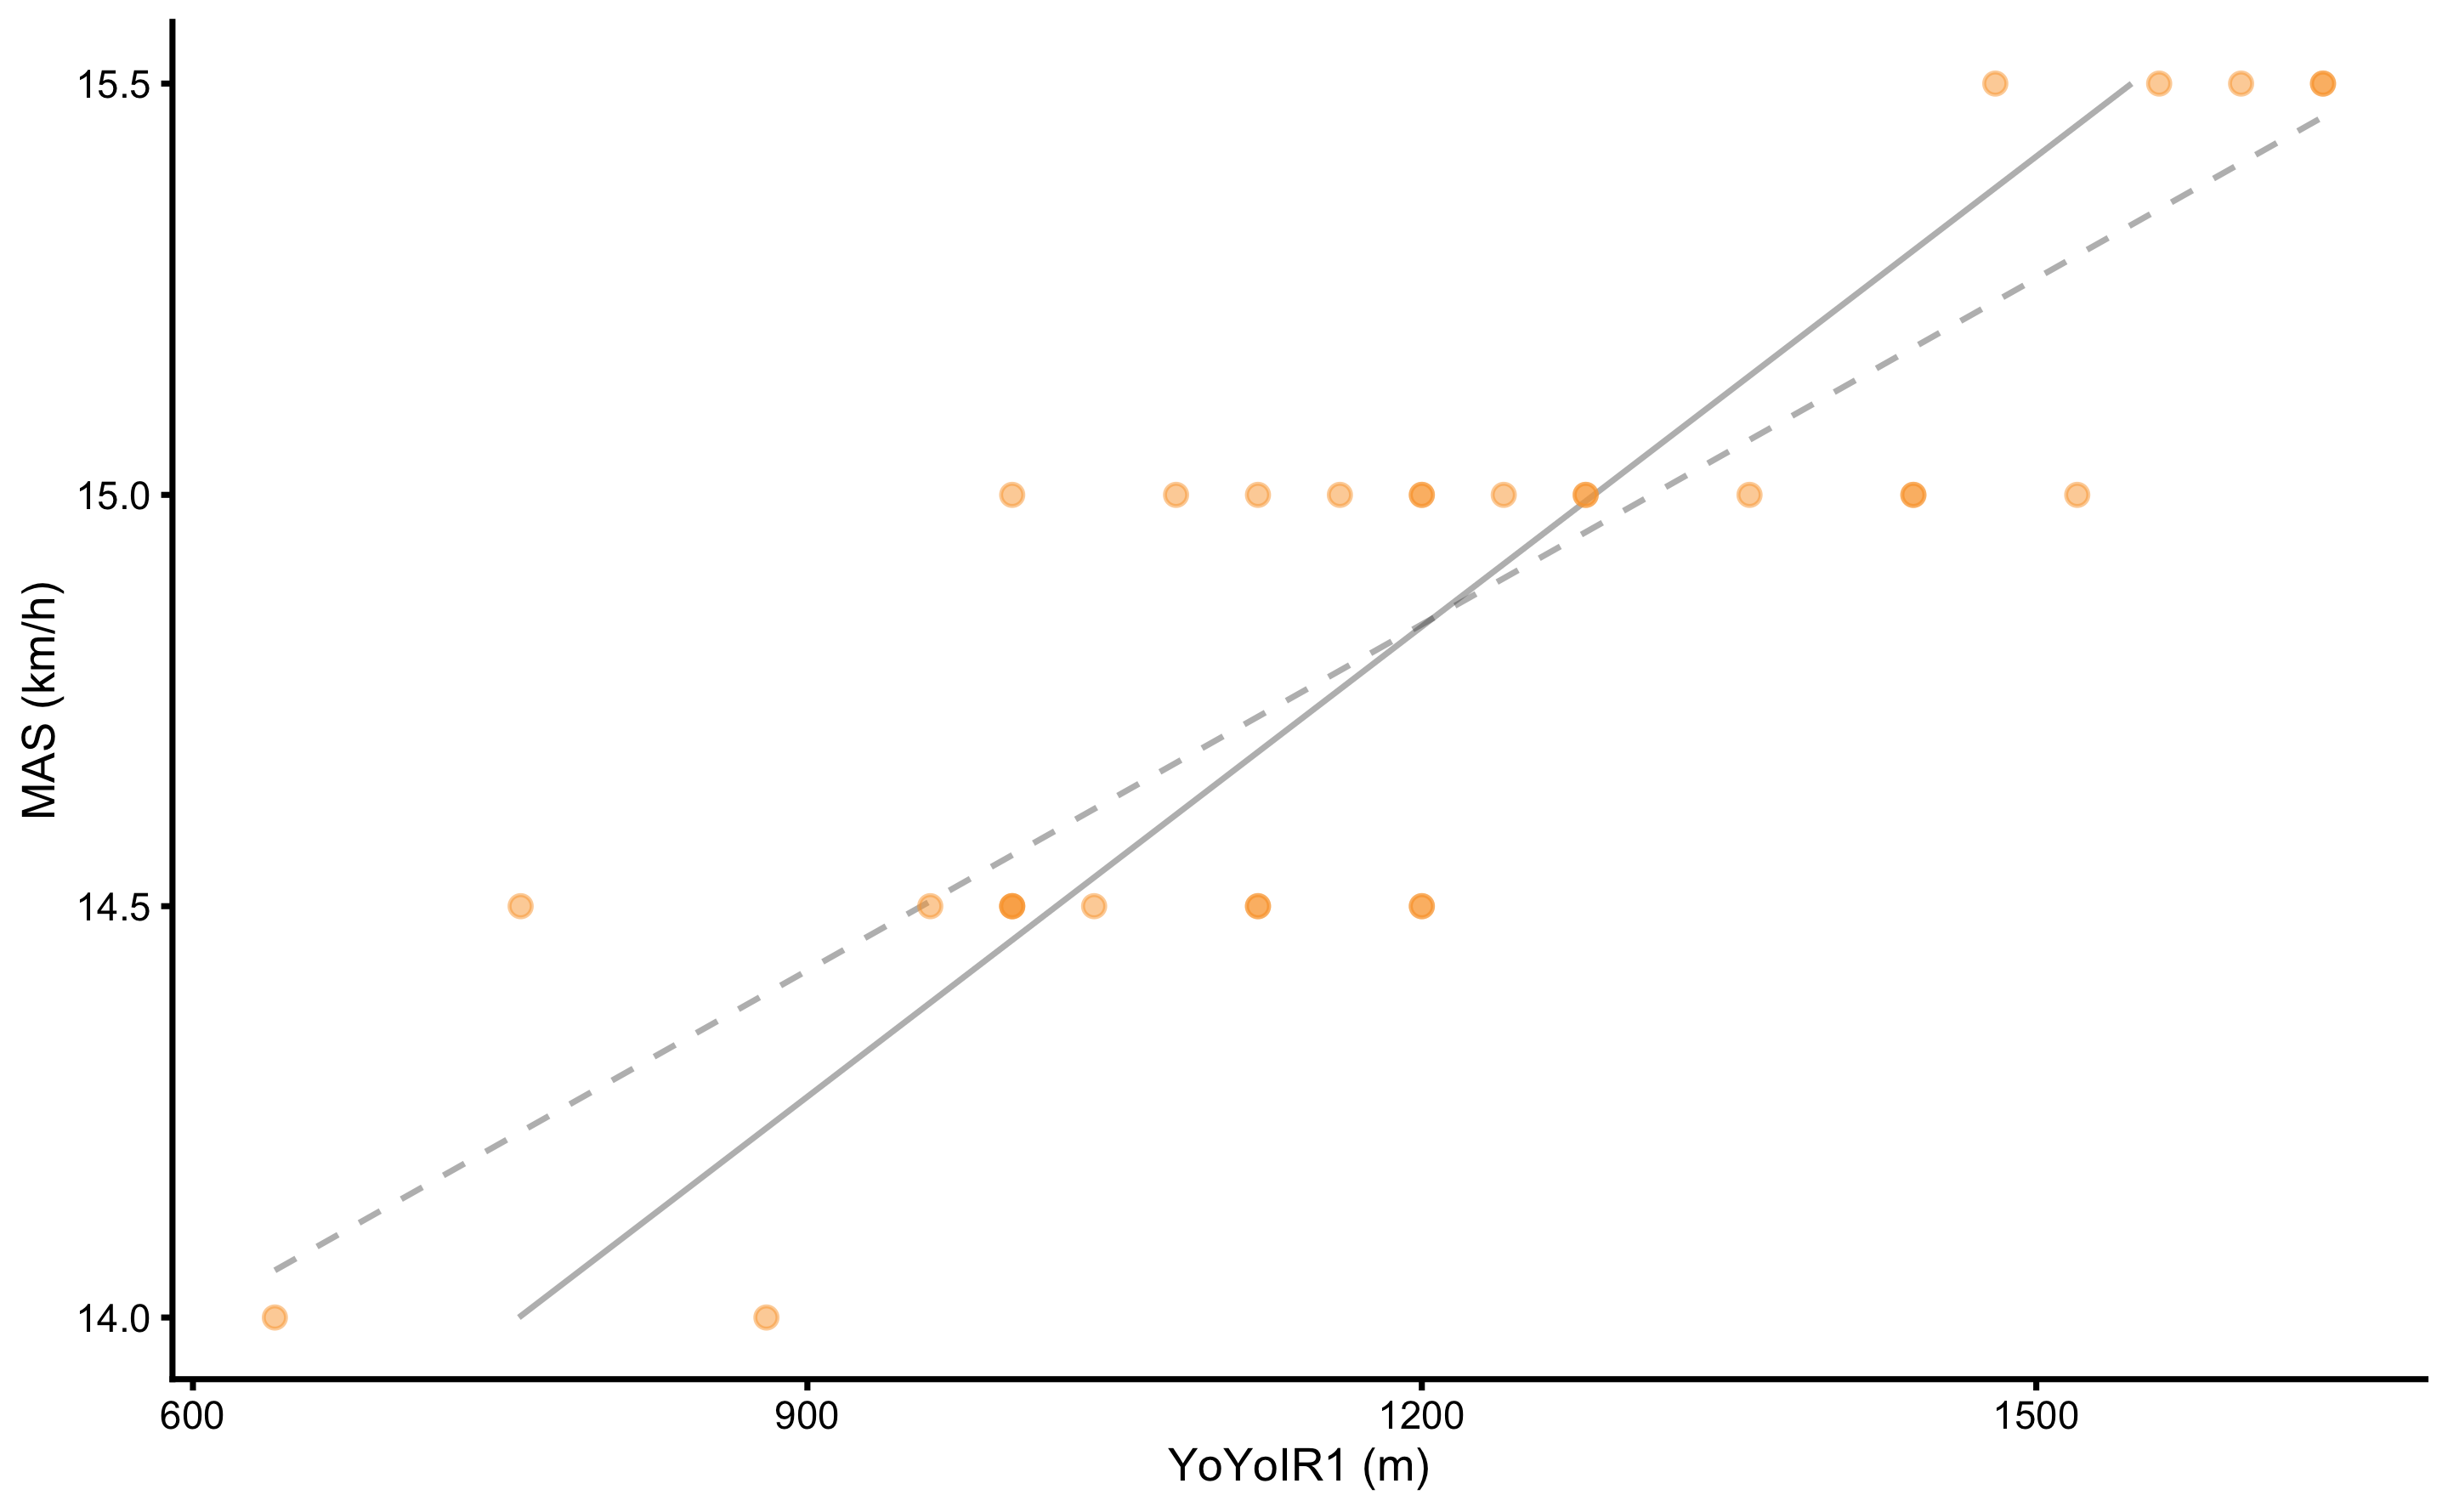
\includegraphics[width=0.9\linewidth]{02-Description_files/figure-latex/reverse-linear-1} 

}

\caption{\textbf{Regression line differs depending which variable is target or the outcome variable. }Dashed grey line represents regression line when MAS is the target variable. Grey line represents regression line when YoYoIR1 is the target variable. Since they are not identical, one cannot reverse the equation to predict YoYoIR1 from MAS score, when such equation is estimated by predicting MAS from YoYoIR1}\label{fig:reverse-linear}
\end{figure}



Unfortunately, this is common practice in sport science. Rather than reversing parameters, one needs to fit, in this case, linear regression model again with the properly defined target and predictor variables. In certain scenarios, such as \protect\hyperlink{reliability}{Reliability} analysis, we do not know which variable represents predictor and which represents target or outcome. For this reason, different approaches to regression, such as \emph{ordinary least products} (OLP) are utilized (Ludbrook \protect\hyperlink{ref-ludbrookLinearRegressionAnalysis2010}{2010}, \protect\hyperlink{ref-ludbrookPrimerBiomedicalScientists2012}{2012}, \protect\hyperlink{ref-ludbrookSPECIALARTICLECOMPARING1997}{1997}, \protect\hyperlink{ref-ludbrookStatisticalTechniquesComparing2002}{2002}; Mullineaux, Barnes, and Batterham \protect\hyperlink{ref-mullineauxAssessmentBiasComparing1999}{1999}). These topics will be covered in the second part of this book.

\hypertarget{magnitude-based-estimators}{%
\subsection{Magnitude-based estimators}\label{magnitude-based-estimators}}

Similarly to independent and dependent group analysis, with association we might be interested in the practical significance of the results. In order to judge results from practical significance perspective, we need to define SESOI of both variables (i.e.~YoYoIR1 and MAS). Using minimal test increment, SESOI for the YoYoIR1 test is defined as ±40m, and SESOI for the MAS test is defined as ±0.5km/h.

One question we might ask is whether the YoYoIR1 SESOI is associated with MAS SESOI. This can be answered with the \texttt{sensitivity} estimator (Equation \eqref{eq:practical-sensitivity}).

\begin{equation}
  \begin{split}
    Sensitivity &= \frac{(SESOI_{YoYoIR1_{upper}} - SESOI_{YoYoIR1_{lower}})\times\hat{\beta}_1}{SESOI_{MAS_{upper}}-SESOI_{MAS_{lower}}} \\
    Sensitivity &= \frac{(40 - -40)\times 0.0014}{0.5--0.5} \\
    Sensitivity &= \frac{(80)\times 0.0014}{1} \\
    Sensitivity &= \frac{0.11}{1} \\
    Sensitivity &= 0.11
  \end{split}
  \label{eq:practical-sensitivity}
\end{equation}

This means that the change in the YoYoIR1 test equal to SESOI will yield only a small proportion of SESOI in the MAS test.

In the case where SESOI of the MAS test is unknown, using known SESOI of the YoYoIR1 test can be used to estimate it. This is done by using estimated \(\hat{\beta}_1\) (\texttt{slope\ coefficient}), as demonstrated in the Equation \eqref{eq:mas-sesoi-equation}.

\begin{equation}
  \begin{split}
    SESOI_{MAS_{upper}} &= \hat{\beta}_1\times SESOI_{YoYoIR1_{upper}} \\
    SESOI_{MAS_{upper}} &= 0.0014\times 40 \\
    SESOI_{MAS_{upper}} &= 0.06 \: km/h \\
    \\
    SESOI_{MAS_{lower}} &= \hat{\beta}_1\times SESOI_{YoYoIR1_{lower}} \\
    SESOI_{MAS_{lower}} &= 0.0014\times -40 \\
    SESOI_{MAS_{lower}} &= -0.06 \: km/h
    \end{split}  
    \label{eq:mas-sesoi-equation}
\end{equation}

Next magnitude-based question might be related to the practically significant strength of the association between two variables. For example, we would like to know if the residuals are higher or lower than the SESOI in the target variable (i.e.~MAS, which is equal to ±0.5km/h). Figure \ref{fig:sesoiscatterplot-mas-yoyo} depicts scatter plot between two variable (panel A) and residuals (panel B) utilizing SESOI in MAS as the grey area.

\begin{figure}[!htb]

{\centering 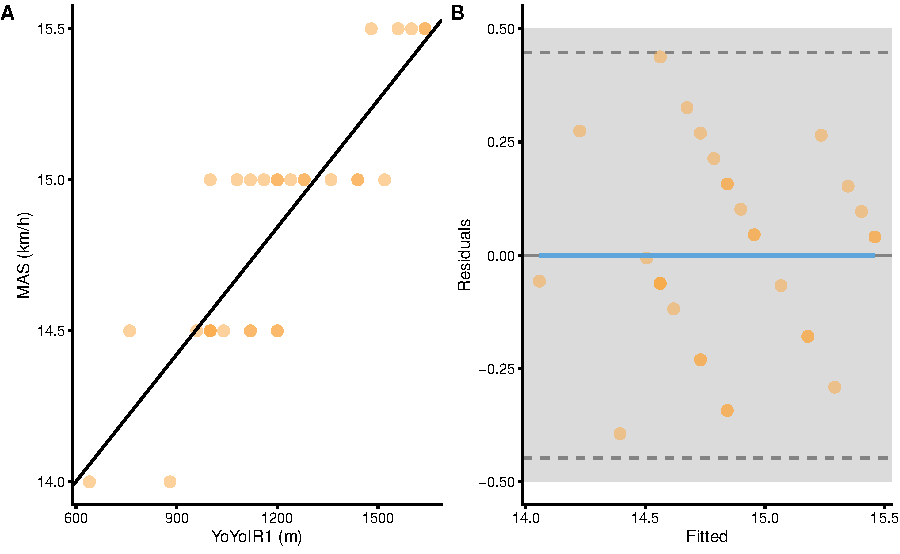
\includegraphics[width=0.9\linewidth]{02-Description_files/figure-latex/sesoiscatterplot-mas-yoyo-1} 

}

\caption{\textbf{Scatter plot between two variables using SESOI to indicate practically significant difference A.} Scatterplot with SESOI depicted as grey band around linear regression line. \textbf{B.} Residual plot, where the difference between MAS and linear regression line (model estimate) is plotted against linear regression line (fitted or predicted MAS). SESOI is represented with the grey band. Residuals within SESOI band are of no practical difference. Dashed lines represent upper and lower \emph{levels of agreement} using \texttt{RSE} and 95\% confidence level (or in other words, 95\% of the residuals distribution will be within these two dashed lines).}\label{fig:sesoiscatterplot-mas-yoyo}
\end{figure}



Magnitude-based estimators of the practically significant strength of the two variable association involve ratio between the SESOI (\(SESOI_{upper} - SESOI_{lower}\)) and \texttt{RSE} (\texttt{SESOI\ to\ RSE}), and \texttt{PPER}. \texttt{SESOI\ to\ RSE} indicates how big are the residuals compared to the SESOI, and thus a metric of the practical strength of the association. Assuming that residuals are being normally distributed, SESOI to RSE over 4 (or \(2\times 1.96\)) would indicate excellent practical strength of the association. If you look at the Table 15, estimated SESOI to RSE in this example is not great, indicating poor practical strength of association.

\emph{Proportion of practically equivalent residuals} (\texttt{PPER}) as a measure of the practical strength of the association revolves around estimating proportions of residuals in the \emph{equivalent} range, defined as SESOI in the target variable (which is exactly the same as already introduced \texttt{pEquivalent} estimator). \texttt{PPER} can be estimated with the brute-force method by simply counting residuals in the equivalent zone, or using algebraic method and assuming normally distributed residuals (i.e.~using \texttt{RSE} of the residuals\footnote{To estimate \texttt{PPER} algebraically, one can use residual \texttt{SD}, \texttt{RSE}, or \texttt{RMSE} since these are all measures of dispersion. In predictive models (see \protect\hyperlink{prediction}{Prediction} section) \texttt{RMSE} is utilized to estimate \texttt{PPER}.}).

Figure \ref{fig:p-equivalent} graphically depicts how \texttt{PPER} is calculated. Practically significant association between two variables would have \texttt{PPER} equal to 1, which indicates that all residuals are within confines of the SESOI. If you look at the Table \ref{tab:association-magnitude-table}, estimated \texttt{PPER} in this example is almost perfect, indicating great practical strength of the association between YoYoIR1 and MAS tests.

\begin{figure}[!htb]

{\centering 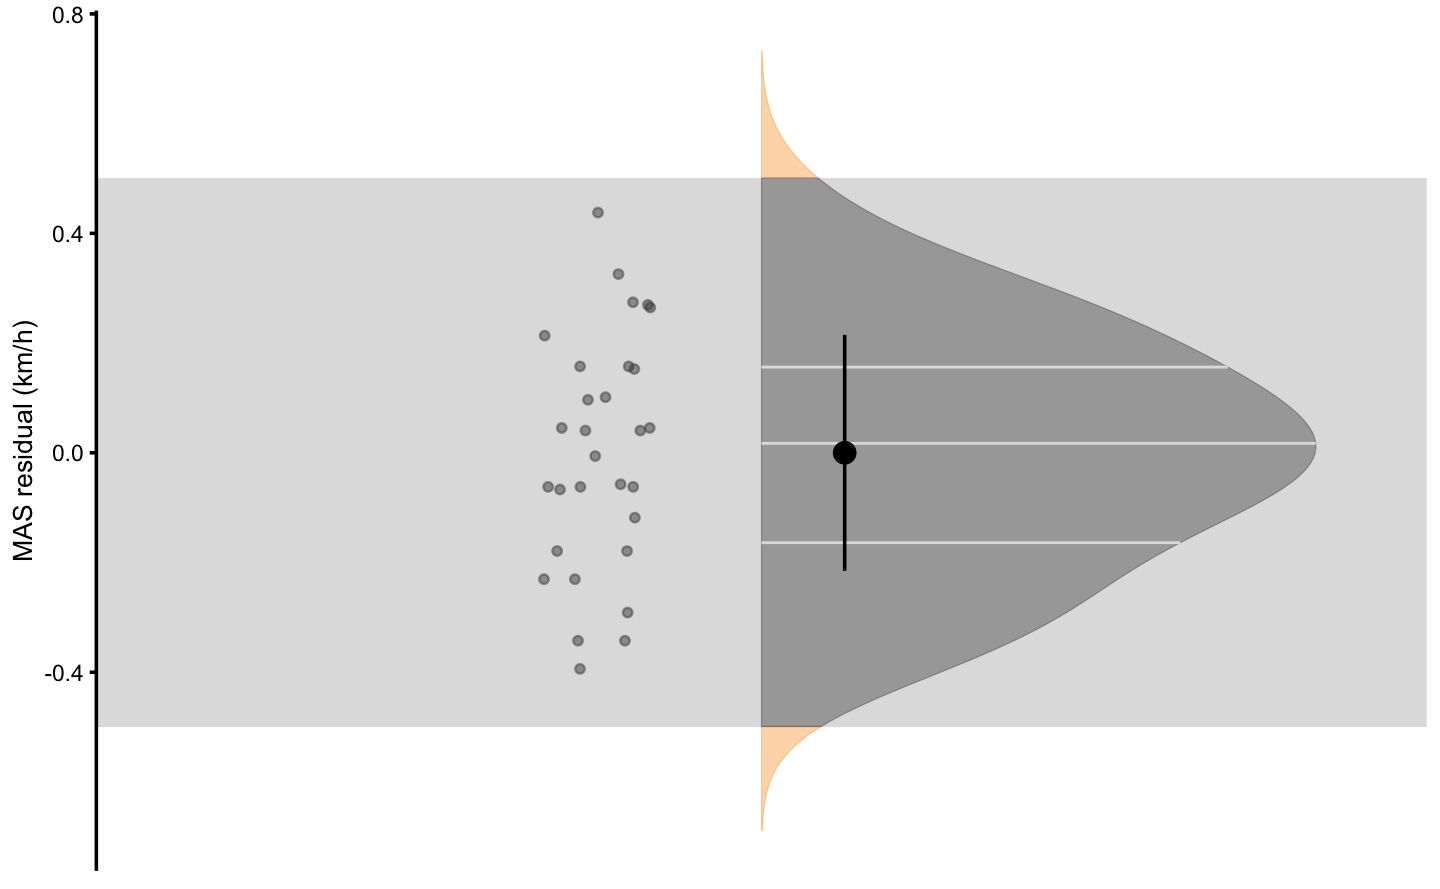
\includegraphics[width=0.9\linewidth]{02-Description_files/figure-latex/p-equivalent-1} 

}

\caption{\textbf{Residuals of the linear regression model predicting MAS from YoYoIR1 test. }Proportion of residuals within SESOI band represent \texttt{PPER}}\label{fig:p-equivalent}
\end{figure}





\begin{table}

\caption{\label{tab:association-magnitude-table}\textbf{Magnitude-based estimators of the association between two variables.} Association is estimated using linear regression model. MAS is the target variable, and YoYoIR1 is the predictor}
\centering
\resizebox{\linewidth}{!}{
\begin{tabular}[t]{llrrrr}
\toprule
SESOI YoYoIR1 (m) & SESOI MAS (km/h) & Sensitivity & RSE & SESOI MAS to RSE & PPER\\
\midrule
±40 & ±0.5 & 0.11 & 0.22 & 4.57 & 0.98\\
\bottomrule
\end{tabular}}
\end{table}

Visual inspection from the Figure \ref{fig:p-equivalent} and magnitude-based estimates from the Table \ref{tab:association-magnitude-table} indicate that using YoYoIR1 test scores, we are able to \emph{predict}\footnote{This is not ideal estimate of the predictive performance of this model as will be explained in the next section on \protect\hyperlink{prediction}{Prediction}.} MAS test scores with the error within SESOI. But would that be the case if the we want to predict YoYoIR1 from MAS test scores? Predictive performance of such model is depicted on the Figure \ref{fig:p-equivalent-for-yoyo} and magnitude-based estimator are enlisted in the Table \ref{tab:association-magnitude-yoyo-table}.

\begin{figure}[!htb]

{\centering 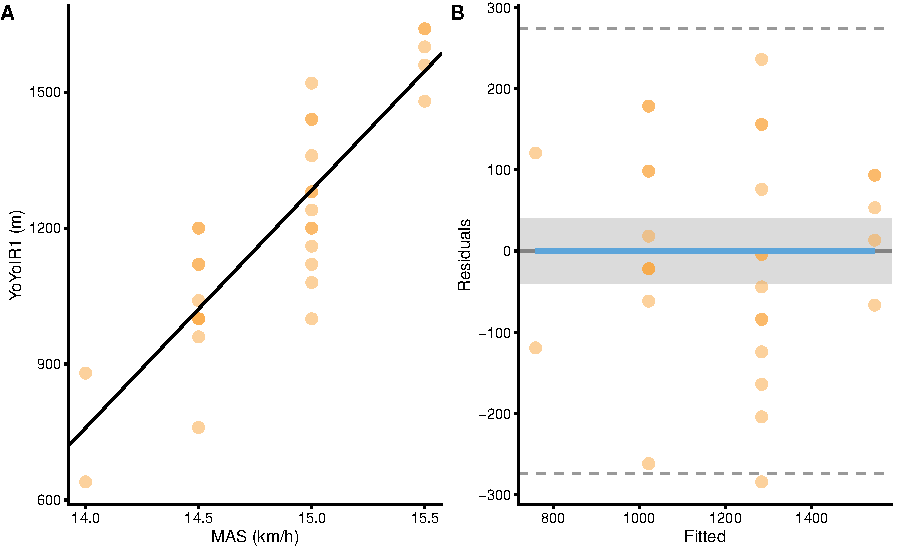
\includegraphics[width=0.9\linewidth]{02-Description_files/figure-latex/p-equivalent-for-yoyo-1} 

}

\caption{\textbf{Linear regression model estimating association between YoYoIR1 and MAS tests where YoYoIR1 is now the target variable. A.} Scatterplot with SESOI depicted as grey band around linear regression line. \textbf{B.} Residual plot, where the difference between YoYoIR1 and linear regression line (model estimate) is plotted against MAS variable. SESOI is represented with the grey band. Residuals within SESOI band are of no practical difference. Proportion of residuals within SESOI band represent \texttt{PPER}}\label{fig:p-equivalent-for-yoyo}
\end{figure}





\begin{table}

\caption{\label{tab:association-magnitude-yoyo-table}\textbf{Magnitude-based estimators of the association between two variables.} Association is estimated using linear regression model. YoYoIR1 is the target variable, and MAS is the predictor}
\centering
\resizebox{\linewidth}{!}{
\begin{tabular}[t]{llrrrr}
\toprule
SESOI YoYoIR1 (m) & SESOI MAS (km/h) & Sensitivity & RSE & SESOI YoYoIR1 to RSE & PPER\\
\midrule
±40 & ±0.5 & 6.56 & 133.84 & 0.6 & 0.23\\
\bottomrule
\end{tabular}}
\end{table}

As clearly indicated with this example, when estimating practical association between two variables, it is very important which variable is the target and which is predictor. When it comes to \texttt{Pearson\textquotesingle{}s\ r}, \texttt{R-Squared} and \texttt{MIC}, this is not the case and results are same regardless of which variable is predictor and which is target.

From the analysis performed, it seems that predicting MAS from YoYoIR1 is practically useful and the association is practically significant. Unfortunately, the same is not the case when we try to predict YoYoIR1 from MAS. This might be due different \emph{physical traits} that determine the test scores. For example, results in the YoYoIR1 test might depend on the traits that include, but are not limited to, same traits important for the MAS test.

The purpose of descriptive analysis is only to describe - further analysis involving answering the \emph{why} questions is in the domain of \emph{explanatory modeling} and \emph{causal inference} (which are covered in the \protect\hyperlink{causal-inference}{Causal inference} section), as well as \protect\hyperlink{advanced-uses}{Advanced uses} of descriptive modeling, such as \emph{latent variable modeling}. What is important to remember is that to describe magnitude-based association, it is important to clearly state which variable is the target and which is the predictor.

\hypertarget{advanced-uses}{%
\section{Advanced uses}\label{advanced-uses}}

Advanced techniques in the descriptive statistics involve dimension reduction, such as \emph{principal component analysis} (PCA), latent variable modeling, such as \emph{factor analysis} (FA), or cluster analysis (Beaujean \protect\hyperlink{ref-beaujeanLatentVariableModeling2014}{2014}; Borsboom \protect\hyperlink{ref-borsboomLatentVariableTheory2008}{2008}; Borsboom, Mellenbergh, and van Heerden \protect\hyperlink{ref-borsboomTheoreticalStatusLatent2003}{2003}; Everitt and Hothorn \protect\hyperlink{ref-everittIntroductionAppliedMultivariate2011}{2011}; Finch and French \protect\hyperlink{ref-finchLatentVariableModeling2015}{2015}; Kabacoff \protect\hyperlink{ref-kabacoffActionDataAnalysis2015}{2015}). These techniques are beyond the scope of this book and the interested readers are directed to references provided.

\hypertarget{prediction}{%
\chapter{Prediction}\label{prediction}}

In many disciplines there is a near-exclusive use of the statistical models for causal inference\footnote{Some authors refer to causal inference as ``explanatory'' modeling (Breiman \protect\hyperlink{ref-breimanStatisticalModelingTwo2001}{2001}; Shmueli \protect\hyperlink{ref-shmueliExplainPredict2010}{2010}; Yarkoni and Westfall \protect\hyperlink{ref-yarkoniChoosingPredictionExplanation2017}{2017}), although Miguel Hernan warns against using such a somewhat-misleading term ``because causal effects may be quantified while remaining unexplained (randomized trials identify causal effects even if the causal mechanisms that explain them are unknown)'' (Hernán, Hsu, and Healy \protect\hyperlink{ref-hernanSecondChanceGet2019}{2019}, 43). Andrew Gelman also makes distinctions between \emph{forward causal inference} and \emph{reverse causal inference} that might be useful in distinguishing between identifying causal effects and explaining them (Gelman \protect\hyperlink{ref-gelmanCausalityStatisticalLearning2011}{2011}). This is elaborated in the \protect\hyperlink{causal-inference}{Causal inference} section of this book.} and the assumption that models with high explanatory power are inherently of high predictive power (Breiman \protect\hyperlink{ref-breimanStatisticalModelingTwo2001}{2001}; Shmueli \protect\hyperlink{ref-shmueliExplainPredict2010}{2010}; Yarkoni and Westfall \protect\hyperlink{ref-yarkoniChoosingPredictionExplanation2017}{2017}; Hernán, Hsu, and Healy \protect\hyperlink{ref-hernanSecondChanceGet2019}{2019}). There is a constant tug-of-war between prediction versus explanation, and experts are leaning on one side or the other. Some experts warn against over-reliance on explanatory models with poor predictive power (Breiman \protect\hyperlink{ref-breimanStatisticalModelingTwo2001}{2001}; Shmueli \protect\hyperlink{ref-shmueliExplainPredict2010}{2010}; Yarkoni and Westfall \protect\hyperlink{ref-yarkoniChoosingPredictionExplanation2017}{2017}), whereas some warn against over-reliance on predictive models that lack causal explanatory power that can guide intervention (Hernán, Hsu, and Healy \protect\hyperlink{ref-hernanSecondChanceGet2019}{2019}; Pearl and Mackenzie \protect\hyperlink{ref-pearlBookWhyNew2018}{2018}; Pearl, Glymour, and Jewell \protect\hyperlink{ref-pearlCausalInferenceStatistics2016}{2016}; Pearl \protect\hyperlink{ref-pearlSevenToolsCausal2019}{2019}).

It is thus important to differentiate between the two and take into account the research question that we are trying to answer. In this book, I define predictive modeling by using definition from Galit Shmueli ``as the process of applying a statistical model or data mining algorithm to data for the purpose of predicting new or future observations'' (Shmueli \protect\hyperlink{ref-shmueliExplainPredict2010}{2010}, 291). Usually this predictive statistical model is treated as a \emph{black box}. Black box approach implies that we are not really interested in underlying mechanism and relationships between the predictor variables, only in predictive performance of the model (Breiman \protect\hyperlink{ref-breimanStatisticalModelingTwo2001}{2001}; Shmueli \protect\hyperlink{ref-shmueliExplainPredict2010}{2010}; Yarkoni and Westfall \protect\hyperlink{ref-yarkoniChoosingPredictionExplanation2017}{2017})

Linear regression model from \protect\hyperlink{describing-relationship-between-two-variables}{Describing relationship between two variables} section already introduced predictive question (``If I know someone's YoYoIR1 score, what would be his or her MAS score? Is the prediction within SESOI?'') to \emph{complement} the association one (``How is YoYoIR1 associated with MAS?''). This section will continue this quest and introduce essential concepts and caveats of the predictive analysis needed to answer predictive questions.

\hypertarget{overfitting}{%
\section{Overfitting}\label{overfitting}}

To explain a few caveats with predictive modeling, let's take slightly more complex example (although we will come back to YoYoIR1 and MAS relationship later). Imagine we know the \emph{true} relationship between back squat \emph{relative 1RM} (BS)\footnote{For example, if an athlete lifted 175kg for a single rep in the back squat, and was unable to lift more, this represents his back squat 1RM, or one repetition maximum. Relative 1RM is calculated by dividing 1RM with athlete's bodyweight. For example, an athlete with 175kg 1RM weights 85kg. His relative 1RM is equal to 2.05.} and vertical jump height during a bodyweight squat jump (SJ; measured in cm). This true relationship is usually referred to as \emph{data generating process} (DGP) (Carsey and Harden \protect\hyperlink{ref-carseyMonteCarloSimulation2013}{2013}) and one of the aims of causal inference tasks is to uncover parameters and mechanism of DGP from the acquired sample\footnote{Uncovering DGP parameters is not solely the goal of the causal inference (although causal inference task is to uncover or quantify causal mechanism), but also the main goal in the statistical inference where the aim is to quantify uncertainty about the \emph{true} population parameters from the acquired sample. More about this topic in the \protect\hyperlink{statistical-inference}{Statistical Inference} section.}. With predictive tasks this aim is of no direct interest, but rather reliable prediction regarding new or unseen observations.

DGP is usually unknown, but with simulations, such as this one, DGP is known and it is used to generate the sample data. Simulation is thus excellent teaching tool, since one can \emph{play} with the problem and understand how the statistical analysis works, since the true DGP is known and can be compared with estimates (Carsey and Harden \protect\hyperlink{ref-carseyMonteCarloSimulation2013}{2013}; Hopkins \protect\hyperlink{ref-hopkinsUnderstandingStatisticsUsing2007}{2007}; Guillaume A Rousselet, Pernet, and Wilcox \protect\hyperlink{ref-rousseletPracticalIntroductionBootstrap2019}{2019}\protect\hyperlink{ref-rousseletPracticalIntroductionBootstrap2019}{a}).

DGP is assumed to consist of \emph{systematic component} \(f(x)\) and \emph{stochastic component} \(\epsilon\) (Equation \eqref{eq:systematic-stochastic}).

\begin{equation}
  Y = f(X) + \epsilon
  \label{eq:systematic-stochastic}
\end{equation}

Systematic component is assumed to be \emph{fixed} in the population (constant from sample to sample) and captures the \emph{true} relationship \(f(X)\) among variables in the population (e.g.~this can also be termed \emph{signal}), while stochastic component represents \emph{random noise} or \emph{random error}, that varies from sample to sample, although its distribution remains the same. Random error is assumed to be normally distributed with mean of 0 and standard deviation which represents estimated parameter (either with \texttt{RMSE} or \texttt{RSE}). Thus, \texttt{RMSE} or \texttt{RSE} are \emph{estimates} of \(\epsilon\).

In our example, the relationship between SJ and BS is expressed with the following Equation \eqref{eq:sj-bs-equation}.

\begin{equation}
  \begin{split}
    SJ &= 30 + 15\times BS\times\sin(BS)+\epsilon \\
    \epsilon &\sim \mathcal{N}(0,\,2)
  \end{split}
  \label{eq:sj-bs-equation}
\end{equation}

Systematic component in the DGP is represented with \(30 + 15\times BS\times\sin(BS)\), and stochastic component is represented with the \emph{known} random error (\(\epsilon\)) that is normally distributed with the mean equal to zero and standard deviation equal to 2cm (\(\mathcal{N}(0,\,2)\)). This random error can be termed \emph{irreducible error} (James et al. \protect\hyperlink{ref-jamesIntroductionStatisticalLearning2017}{2017}), since it is inherent to the true DGP. As will be demonstrated shortly, models that perform better than this irreducible error are said to \emph{overfit}. In other words, models are jumping to the noise.

The objective of causal inference or explanatory modeling is to estimate the \(f(X)\) (estimate is indicated with the \emph{hat} symbol: \(\hat{f}(x)\)) or to understand the underlying DGP. With the predictive analysis, the goal is to find the best estimate of \(Y\) or \(\hat{y}\). The underlying DGP is treated as a \emph{black box}.

To demonstrate a concept of overfitting, we are going to generate two samples (N=35 observations) from the DGP with BS ranging from 0.8 to 2.5. These samples are \emph{training} and \emph{testing} sample (Figure \ref{fig:bs-sj-training-testing}). Training sample is used to \emph{train} the prediction model, while \emph{testing} sample will be used as a \emph{holdout} sample for evaluating model performance on the \emph{unseen} data.

\begin{figure}[!htb]

{\centering 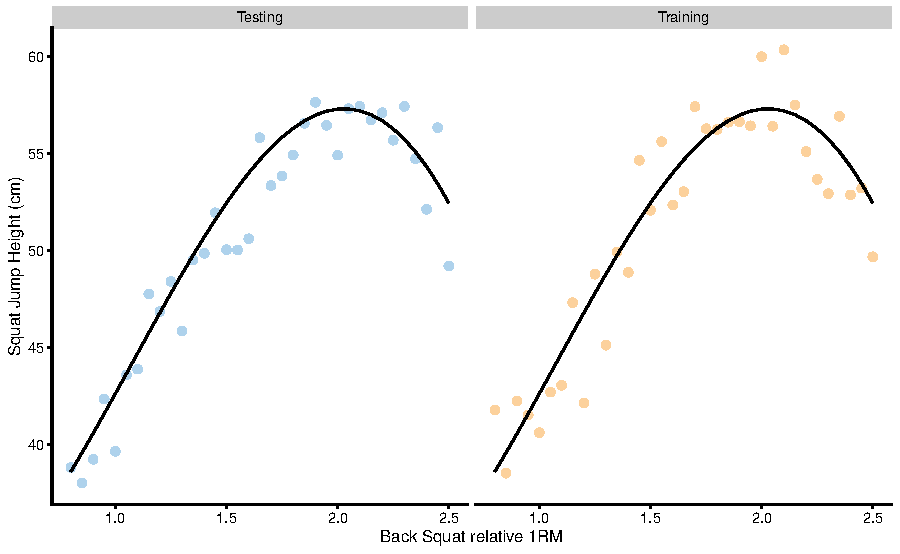
\includegraphics[width=0.9\linewidth]{03-Prediction_files/figure-latex/bs-sj-training-testing-1} 

}

\caption{\textbf{Two samples simulated from the known DGP. }Black line represents systematic component of the DGP and it is equal for both training and testing samples. Observations vary in the two samples due stochastic component in the DGP}\label{fig:bs-sj-training-testing}
\end{figure}



Model used to predict SJ from BS will be \emph{polynomial linear regression}. Equation \eqref{eq:polynomial-equation} explains first, second, and third degree polynomial linear regression function and provides a form for n-degree polynomials. Please, note that first degree polynomial function represents simple linear regression.

\begin{equation}
  \begin{split}
    \hat{y_i} &= \hat{\beta}_0 + \hat{\beta}_1 x_i^1 \\
    \hat{y_i} &= \hat{\beta}_0 + \hat{\beta}_1 x_i^1 + \hat{\beta}_2 x_i^2 \\
    \hat{y_i} &= \hat{\beta}_0 + \hat{\beta}_1 x_i^1 + \hat{\beta}_2 x_i^2 + \hat{\beta}_3 x_i^3 \\
    \hat{y_i} &= \hat{\beta}_0 + \hat{\beta}_1 x_i^1 + \dots + \hat{\beta}_n x_i^n
  \end{split}
  \label{eq:polynomial-equation}
\end{equation}

Increasing polynomial degrees increases the \emph{flexibility} of the polynomial regression model, and thus can represent \emph{tuning parameter} that we can select based on the model performance. In other words, we might be interested in finding polynomial degree that minimized model error (or maximize model fit). Figure \ref{fig:poly-fit-model} contains model performance on the training data for polynomial degrees ranging from 1 to 20.

\begin{figure}[!htb]

{\centering 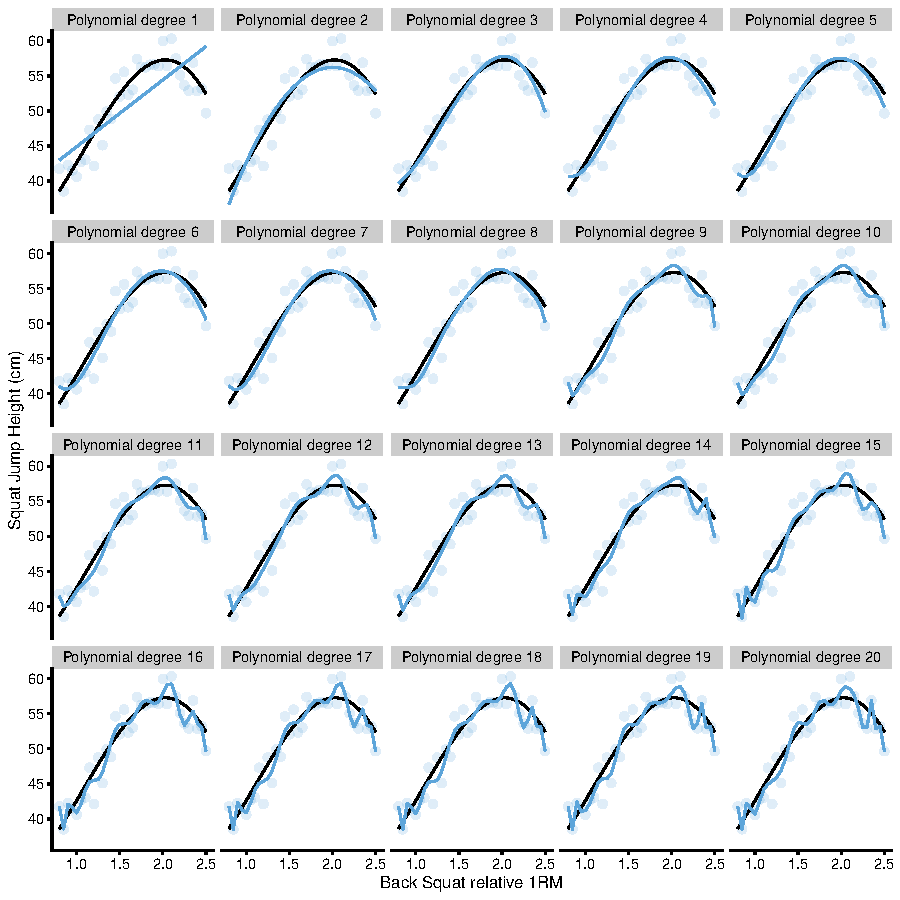
\includegraphics[width=0.9\linewidth]{03-Prediction_files/figure-latex/poly-fit-model-1} 

}

\caption{\textbf{Model fit with varying polynomial degrees. }More degrees equals better model fit}\label{fig:poly-fit-model}
\end{figure}



As can be seen from the Figure \ref{fig:poly-fit-model}, the more flexible the model (or the higher the polynomial degree) the better it fits the data. But how do these models perform on the unseen, testing data sample? In order to quantify model performance, \texttt{RMSE} metric is used. Figure \ref{fig:testing-training-poly-errors} demonstrates performance of the polynomial regression model on the training and testing data sample across different polynomial degrees.

\begin{figure}[!htb]

{\centering 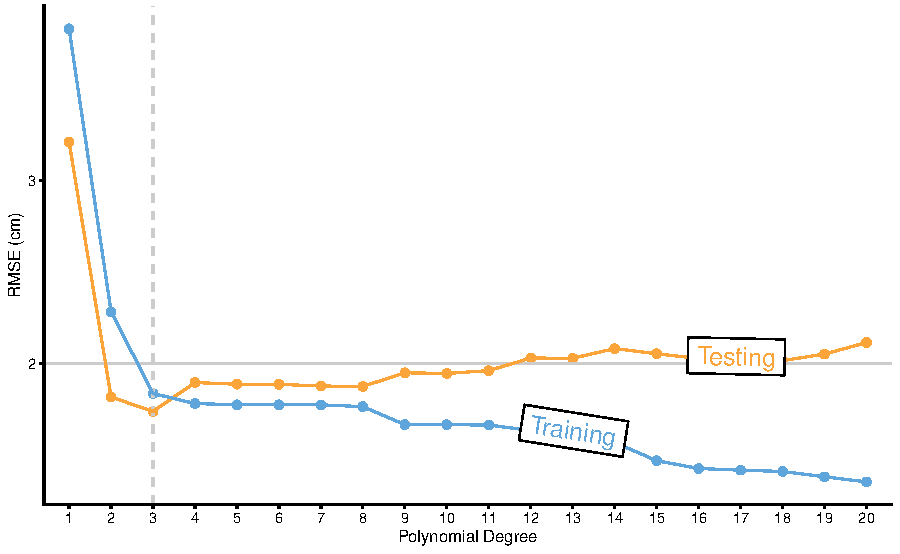
\includegraphics[width=0.9\linewidth]{03-Prediction_files/figure-latex/testing-training-poly-errors-1} 

}

\caption{\textbf{Testing and training errors across varying polynomial degrees. }Model error is estimated with the \texttt{RMSE} metric, while polynomial degree represents tuning or flexibility parameter of the model. As can be noted from the figure, better training performance doesn't imply better testing performance. Vertical dashed line represents the polynomial degree at which testing error is lowest. Polynomial degrees on the right of the vertical dashed line are said to overfit the data, while polynomial degree on the left are said to underfit the data}\label{fig:testing-training-poly-errors}
\end{figure}



As can be seen from the Figure \ref{fig:testing-training-poly-errors}, models with higher polynomial degrees tend to overfit (indicated by performance better than the known irreducible error \(\epsilon\) visualized with the horizontal line at 2cm). Performance on the training data sample improves as the polynomial degrees increase, which is not the case with the performance on the testing data sample. There is clearly the best polynomial degree that has the best predictive performance on the unseen data. Polynomial degrees on the left of the vertical dashed line are said to \emph{underfit}, while polynomial degrees on the right are said to overfit.

The take home message is that predictive performance on the training data can be too optimistic, and for evaluating predictive performance of the model, unseen data must be used, otherwise the model might overfit.

\hypertarget{cross-validation}{%
\section{Cross-Validation}\label{cross-validation}}

In order to evaluate predictive performance of the model, researchers usually remove some percent of data to be used as a testing or holdout sample. Unfortunately, this is not always possible (although it is recommended, particularly to evaluate final model performance, especially when there are multiple models and model tuning). One solution to these problems is \emph{cross-validation} technique (James et al. \protect\hyperlink{ref-jamesIntroductionStatisticalLearning2017}{2017}; Kuhn and Johnson \protect\hyperlink{ref-kuhnAppliedPredictiveModeling2018}{2018}; Yarkoni and Westfall \protect\hyperlink{ref-yarkoniChoosingPredictionExplanation2017}{2017}). There are numerous variations of the cross-validation, but the simplest one is \emph{n-fold} cross validation (Figure 15). N-fold cross validation involve splitting the data into 5 to 10 equal folds and using one fold as a testing or hold-out sample while performing model training on the other folds. This is repeated over N-iteration (in this case 5 to 10) and the model performance is averaged to get \emph{cross-validated model performance}.

\begin{figure}[!htb]

{\centering 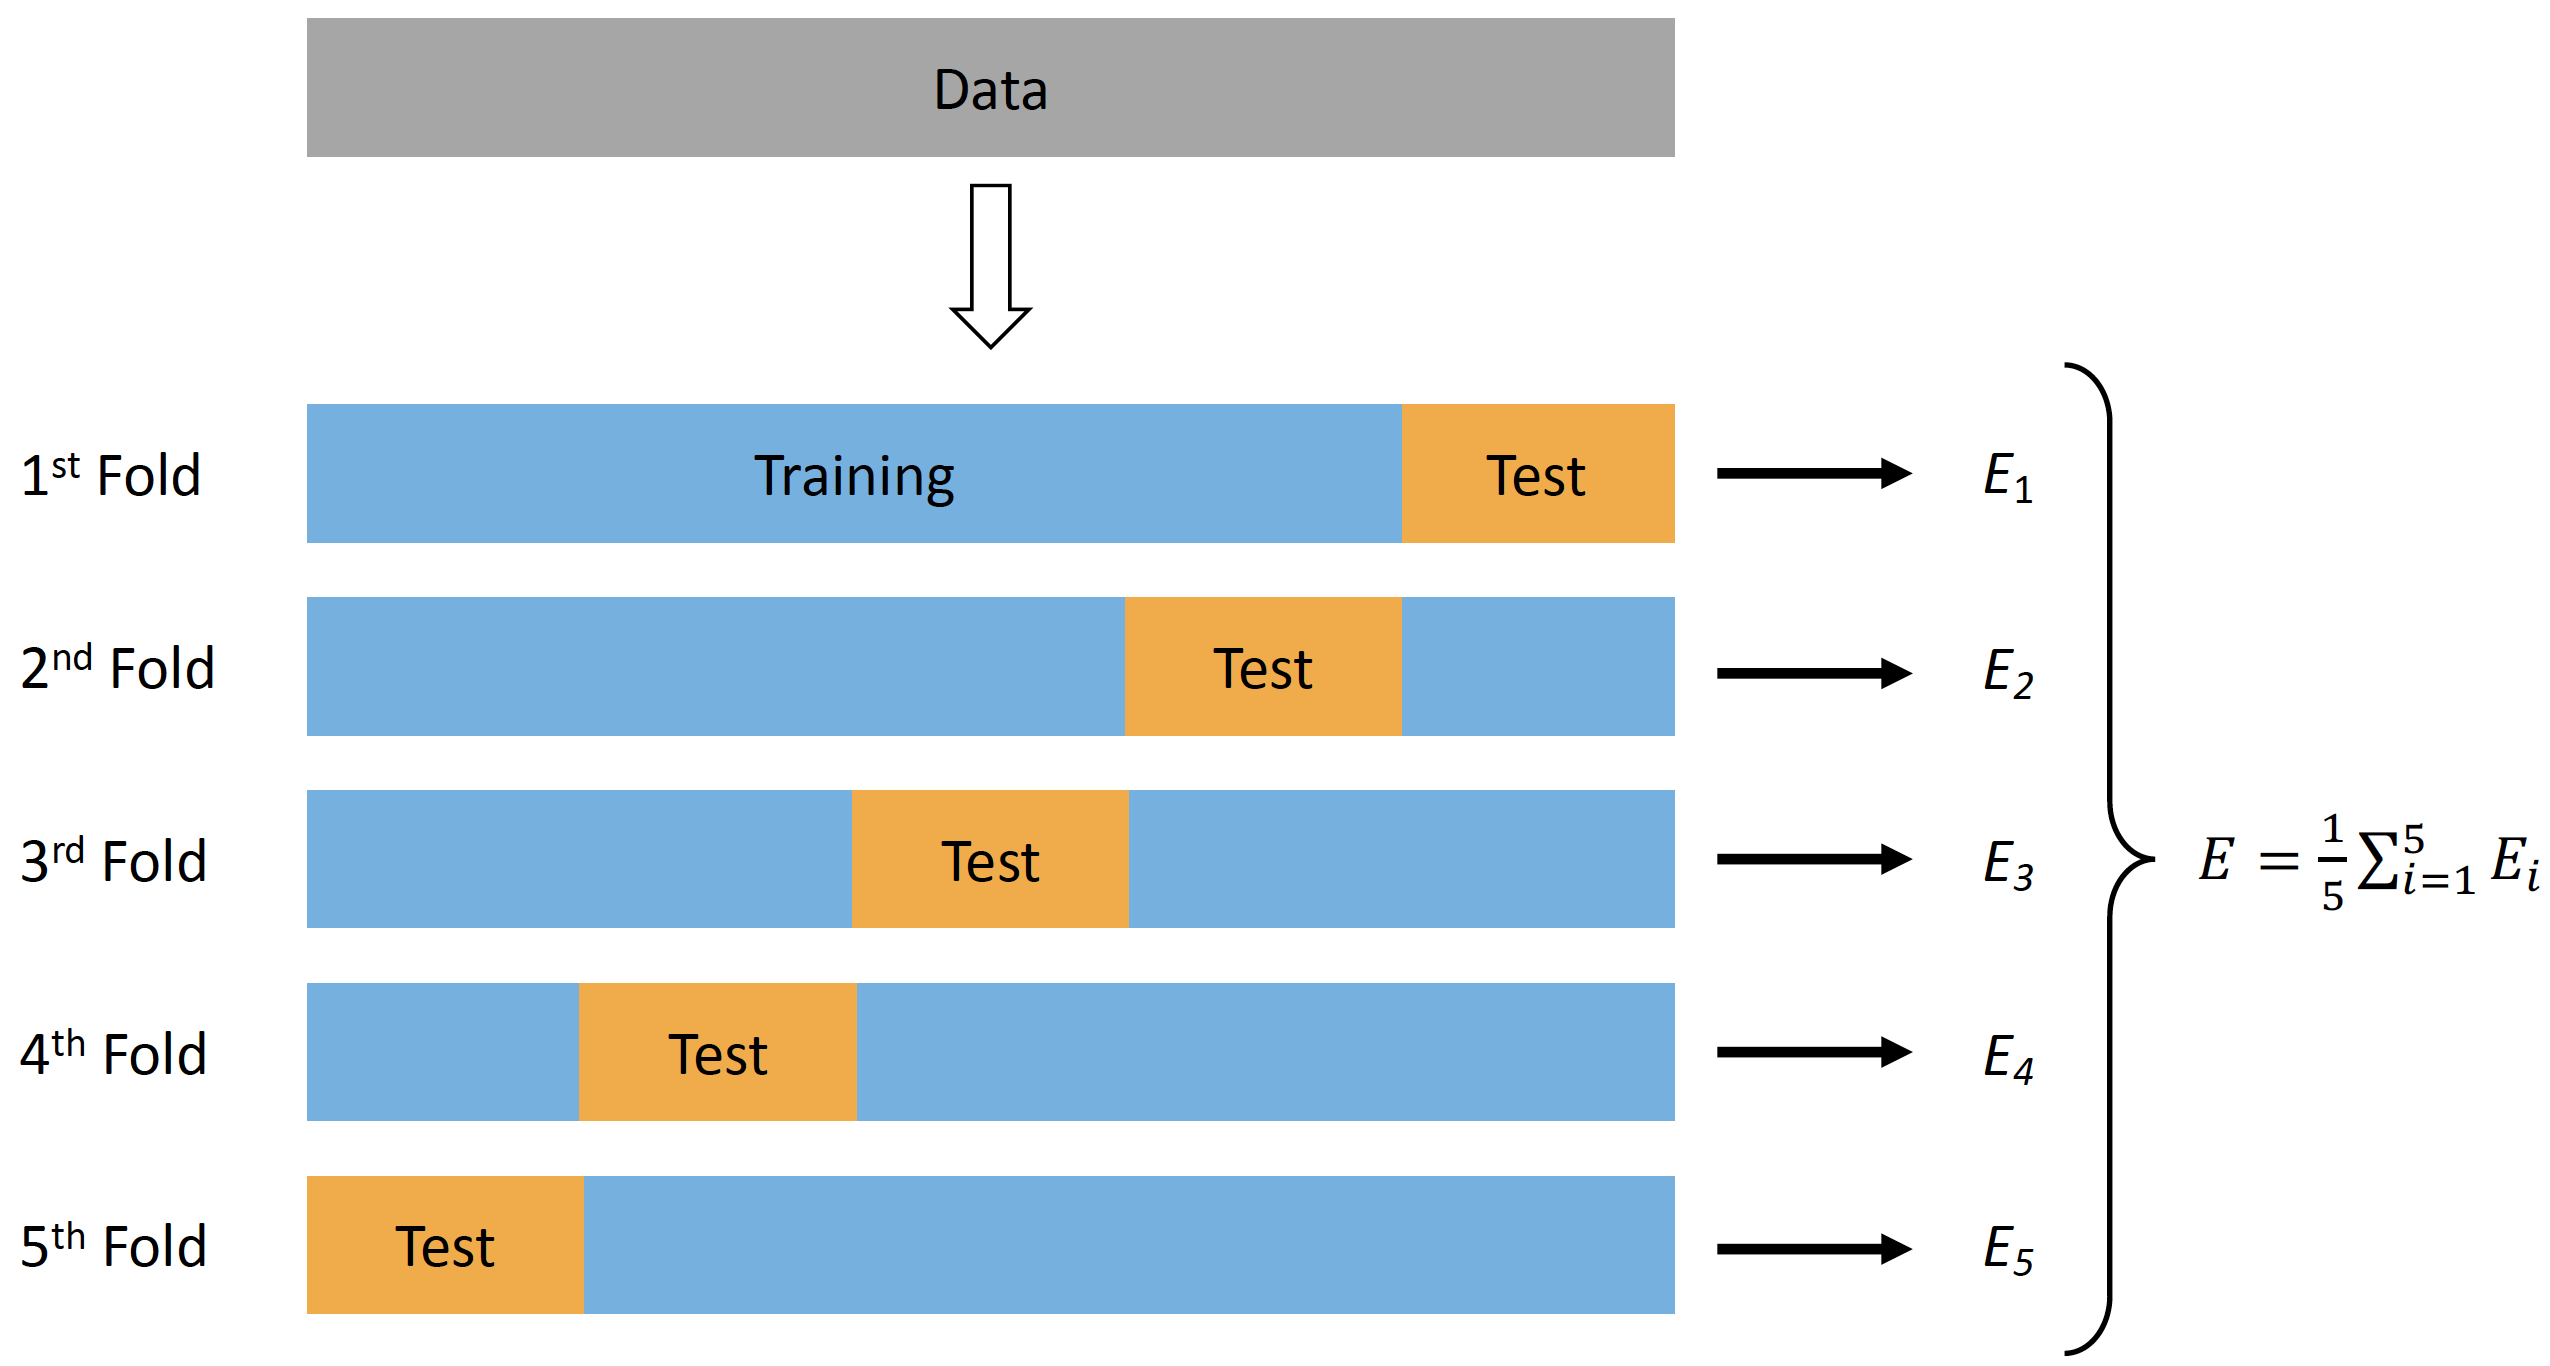
\includegraphics[width=0.9\linewidth]{figures/cross-validation} 

}

\caption{\textbf{Cross-Validation}}\label{fig:cross-validation}
\end{figure}



With predictive analysis and \emph{machine learning}, different model's tuning parameters are evaluated (as well as multiple different models) to estimate the one that gives the best predictive performance. It is thus important to utilize techniques such as cross-validation to avoid overfitting and too optimistic model selection.

Certain models, such as \emph{lasso}, \emph{ridge regression}, and \emph{elastic-net} implement \emph{regularization} parameters that \emph{penalizes} the model complexity and are used as a tuning variable (James et al. \protect\hyperlink{ref-jamesIntroductionStatisticalLearning2017}{2017}; Kuhn and Johnson \protect\hyperlink{ref-kuhnAppliedPredictiveModeling2018}{2018}; Yarkoni and Westfall \protect\hyperlink{ref-yarkoniChoosingPredictionExplanation2017}{2017}). This is useful in situations when there are a lot of predictors, and it is easy to overfit the model. Selecting the best regularization parameter that has the best cross-validated performance helps in simplifying the model and avoiding the overfit. These topics are beyond the scope of this book, and interested readers are directed to references provided.

\hypertarget{sample-mean-as-the-simplest-predictive-model}{%
\subsection{\texorpdfstring{Sample \texttt{mean} as the simplest predictive model}{Sample mean as the simplest predictive model}}\label{sample-mean-as-the-simplest-predictive-model}}

We have already discussed in \protect\hyperlink{sample-mean-as-the-simplest-statistical-model}{Sample \texttt{mean} as the simplest statistical model} section that sample \texttt{mean} can be considered simplest model that describes a particular sample with the lowest \texttt{RMSE}. But can it be used for prediction?

Here is an example to demonstrate both sample \texttt{mean} as a predictive model, as well as to demonstrate cross-validation technique. Let's assume that we have collected N=10 observations: 15, 19, 28, 28, 30, 57, 71, 88, 95, 97. Sample \texttt{mean} is equal to 52.8. If we assume that the sample \texttt{mean} represents our prediction for the observations, we can easily calculate \emph{prediction error} for each observation, which is simple difference (column \texttt{Error} in the Table \ref{tab:mean-as-prediction-differences}).



\begin{table}

\caption{\label{tab:mean-as-prediction-differences}\textbf{Sample \texttt{mean} as prediction with associated prediction errors}}
\centering
\begin{tabular}[t]{rrrrr}
\toprule
Observed & Predicted & Error & Absolute Error & Squared Error\\
\midrule
15 & 52.8 & 37.8 & 37.8 & 1428.84\\
19 & 52.8 & 33.8 & 33.8 & 1142.44\\
28 & 52.8 & 24.8 & 24.8 & 615.04\\
28 & 52.8 & 24.8 & 24.8 & 615.04\\
30 & 52.8 & 22.8 & 22.8 & 519.84\\
\addlinespace
57 & 52.8 & -4.2 & 4.2 & 17.64\\
71 & 52.8 & -18.2 & 18.2 & 331.24\\
88 & 52.8 & -35.2 & 35.2 & 1239.04\\
95 & 52.8 & -42.2 & 42.2 & 1780.84\\
97 & 52.8 & -44.2 & 44.2 & 1953.64\\
\bottomrule
\end{tabular}
\end{table}

Besides simple difference, Table \ref{tab:mean-as-prediction-differences} provides errors (or losses) using two common \emph{loss functions} (see \protect\hyperlink{sample-mean-as-the-simplest-statistical-model}{Sample \texttt{mean} as the simplest statistical model} section in \protect\hyperlink{description}{Description} chapter): \emph{absolute loss} (column \texttt{Absolute\ Error}) and \emph{quadratic loss} (column \texttt{Squared\ Error}).

We need to \emph{aggregate} these errors or losses into a single metric using the \emph{cost function}. If we calculate the mean of the prediction errors (column \texttt{Error} in the Table \ref{tab:mean-as-prediction-differences}), we are going to get 0. This is because the positive and negative errors cancel each other out for the sample \texttt{mean} estimator. This error estimator is often referred to as \emph{mean bias error} (\texttt{MBE}) or simply \emph{bias} and is often used in \emph{validity} and \emph{reliability} analysis (see \protect\hyperlink{validity}{Validity} and \protect\hyperlink{reliability}{Reliability} sections).

If we take the mean of the absolute prediction errors (column \texttt{Absolute\ error} in the Table \ref{tab:mean-as-prediction-differences}) we are going to get \emph{mean absolute error} (\texttt{MAE}) estimator, which is in this example equal to 28.8.

If we take the mean of the squared prediction errors (column \texttt{Squared\ error} in the Table \ref{tab:mean-as-prediction-differences}) we are going to get \emph{mean square error} (\texttt{MSE}) estimator, often called \emph{variance} in the case of describing sample dispersion. In this example \texttt{MSE} is equal to 964.36. To \emph{bring} back \texttt{MSE} to the same scale with the observation scale, square root of the \texttt{MSE} is taken. This represents \emph{root mean square error} (\texttt{RMSE}), which is equal to 31.05. As explained in \protect\hyperlink{sample-mean-as-the-simplest-statistical-model}{Sample \texttt{mean} as the simplest statistical model} section, sample \texttt{mean} represents statistical model of the central tendency with the lowest \texttt{RMSE}.

Aforementioned error estimators, \texttt{MBE}, \texttt{MAE}, \texttt{MSE}, and \texttt{RMSE} can be considered different \emph{cost functions}. Which one should be used\footnote{As explained in \protect\hyperlink{introduction}{Introduction} section, I will mostly focus at variables on continuous ratio scale. Prediction error metrics differ for target variable that is on nominal scale (i.e.~\emph{classification} task) and involve estimators such as \texttt{accuracy}, \texttt{specificity}, \texttt{sensitivity}, \emph{area under curve} (\texttt{AUC}) (Kuhn and Johnson \protect\hyperlink{ref-kuhnAppliedPredictiveModeling2018}{2018}; Lantz \protect\hyperlink{ref-lantzMachineLearningExpert2019}{2019}).}? As always, it depends (Chai and Draxler \protect\hyperlink{ref-chaiRootMeanSquare2014}{2014}). Assuming Gaussian normal distribution of the errors, \texttt{MSE} and \texttt{RMSE} have very useful mathematical properties that can be utilized in modeling stochastic or random components (i.e.~\emph{random error propagation} and prediction error decomposition in \protect\hyperlink{bias-variance-decomposition-and-trade-off}{Bias-Variance decomposition and trade-off} section). This property will be utilized thorough this book and particularly in the \protect\hyperlink{example-of-randomized-control-trial}{Example of randomized control trial} section when estimating random or stochastic component of the treatment effect. I personally prefer to report multiple estimators, including error estimators, which is also a strategy suggested by Chai and Draxler (\protect\hyperlink{ref-chaiRootMeanSquare2014}{2014}).

The are, of course, other loss and cost functions that could be used. For example, one might only use the \emph{maximal error} (\texttt{MaxErr}) and \emph{minimal error} (\texttt{MinErr}), rather than average. Discussion and review of these different metrics is beyond the scope of this book (for more information please check the package \emph{Metrics} (Hamner and Frasco \protect\hyperlink{ref-R-Metrics}{2018}) and the following references (Botchkarev \protect\hyperlink{ref-botchkarevNewTypologyDesign2019}{2019}; Chai and Draxler \protect\hyperlink{ref-chaiRootMeanSquare2014}{2014}; Willmott and Matsuura \protect\hyperlink{ref-willmottAdvantagesMeanAbsolute2005}{2005}; Barron \protect\hyperlink{ref-barronGeneralAdaptiveRobust2019}{2019})). Figure \ref{fig:loss-function-metrics-example} visualize the most common loss functions that are used in both model training and as \emph{performance metrics}. It is important to keep in mind that in the case of OLS regression, \texttt{MSE} (or \texttt{RMSE}) is minimized. It is thus important to make a distinction between cost function used in the optimization and model training (i.e.~in OLS, parameters of the model are found so that \texttt{MSE} is minimized; in some machine-learning models \texttt{Huber\ loss} or \texttt{Rigde\ loss}\footnote{Although I've used the term \emph{loss} here, these loss functions are also aggregated using \texttt{sum} or \texttt{mean} to create \texttt{Huber\ cost} or \texttt{Ridge\ cost}. \texttt{Huber\ loss} is a combination of absolute and quadratic losses and it's property is better \emph{robustness} to outliers.} is minimized; see Figure \ref{fig:loss-function-metrics-example}) versus cost function used as a performance metric (e.g.~reporting \texttt{pEquivalent}, \texttt{MaxErr} or \texttt{MinErr} for OLS models).

\begin{figure}[!htb]

{\centering 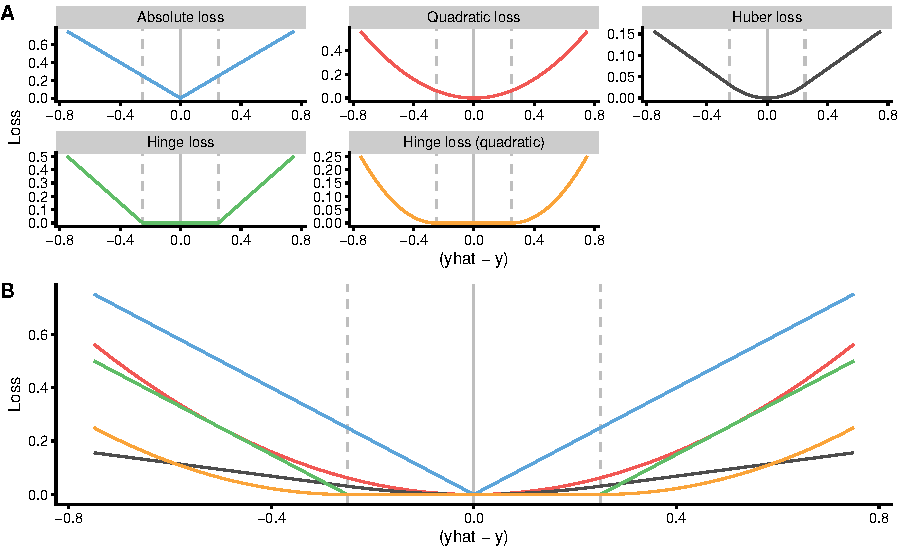
\includegraphics[width=0.9\linewidth]{03-Prediction_files/figure-latex/loss-function-metrics-example-1} 

}

\caption{\textbf{Common loss functions. A. } Trellis plot of each loss function. \textbf{B.} Plot of all loss functions on a common scale. \emph{Huber loss} is a combination of absolute and quadratic loss.}\label{fig:loss-function-metrics-example}
\end{figure}



The take-away point is to understand that there are multiple performance metrics that can be utilized and it is best to report multiple of them.

Estimates for \texttt{MBE}, \texttt{MAE}, \texttt{MSE}\footnote{\texttt{MSE} will be removed from the further analysis and tables since it is equivalent to RMSE, just squared.}, and \texttt{RMSE} represent \emph{training sample} predictive performance since sample \texttt{mean} is estimated using this very sample. We are interested how sample \texttt{mean}, as predictive model, perform on the unseen data. Cross-validation is one method to estimate model performance on unseen data. Table \ref{tab:mean-cross-validation} contains 3-fold cross-validation sample used to train the model (in this case estimate sample \texttt{mean}) and to evaluate the performance on unseen data.



\begin{table}

\caption{\label{tab:mean-cross-validation}\textbf{Example cross-validation using sample \texttt{mean} as the prediction model}}
\centering
\resizebox{\linewidth}{!}{
\begin{tabular}[t]{rlrlrrrrr}
\toprule
Fold & Training sample & mean & Testing Sample & MBE & MAE & RMSE & MinErr & MaxErr\\
\midrule
1 & 15  19  28  --  30  --  71  88  95  -- & 49.43 & --  --  --  28  --  57  --  --  --  97 & -11.24 & 25.52 & 30.44 & -47.57 & 21.43\\
2 & 15  19  --  28  --  57  --  88  --  97 & 50.67 & --  --  28  --  30  --  71  --  95  -- & -5.33 & 27.00 & 28.81 & -44.33 & 22.67\\
3 & --  --  28  28  30  57  71  --  95  97 & 58.00 & 15  19  --  --  --  --  --  88  --  -- & 17.33 & 37.33 & 37.73 & -30.00 & 43.00\\
\bottomrule
\end{tabular}}
\end{table}

Since this is a small sample, we can repeat cross-validation few times. This is called \emph{repeated cross-validation}. Let's repeat 3-folds cross-validation for 5 repeats (Table \ref{tab:repeated-cross-validation}).



\begin{table}

\caption{\label{tab:repeated-cross-validation}\textbf{Example repeated cross-validation using sample \texttt{mean} as the prediction model}}
\centering
\resizebox{\linewidth}{!}{
\begin{tabular}[t]{rrlrlrrrrr}
\toprule
Repeat & Fold & Training sample & mean & Testing Sample & MBE & MAE & RMSE & MinErr & MaxErr\\
\midrule
1 & 1 & 15  19  28  --  30  --  71  88  95  -- & 49.43 & --  --  --  28  --  57  --  --  --  97 & -11.24 & 25.52 & 30.44 & -47.57 & 21.43\\
1 & 2 & 15  19  --  28  --  57  --  88  --  97 & 50.67 & --  --  28  --  30  --  71  --  95  -- & -5.33 & 27.00 & 28.81 & -44.33 & 22.67\\
1 & 3 & --  --  28  28  30  57  71  --  95  97 & 58.00 & 15  19  --  --  --  --  --  88  --  -- & 17.33 & 37.33 & 37.73 & -30.00 & 43.00\\
2 & 1 & --  19  28  --  30  57  71  88  --  -- & 48.83 & 15  --  --  28  --  --  --  --  95  97 & -9.92 & 37.25 & 38.83 & -48.17 & 33.83\\
2 & 2 & 15  --  28  28  --  57  --  --  95  97 & 53.33 & --  19  --  --  30  --  71  88  --  -- & 1.33 & 27.50 & 28.45 & -34.67 & 34.33\\
\addlinespace
2 & 3 & 15  19  --  28  30  --  71  88  95  97 & 55.38 & --  --  28  --  --  57  --  --  --  -- & 12.87 & 14.50 & 19.39 & -1.63 & 27.37\\
3 & 1 & --  19  28  28  30  57  71  88  --  -- & 45.86 & 15  --  --  --  --  --  --  --  95  97 & -23.14 & 43.71 & 44.66 & -51.14 & 30.86\\
3 & 2 & 15  19  --  --  30  --  --  88  95  97 & 57.33 & --  --  28  28  --  57  71  --  --  -- & 11.33 & 18.17 & 21.84 & -13.67 & 29.33\\
3 & 3 & 15  --  28  28  --  57  71  --  95  97 & 55.86 & --  19  --  --  30  --  --  88  --  -- & 10.19 & 31.62 & 31.94 & -32.14 & 36.86\\
4 & 1 & --  19  28  --  30  57  71  88  --  97 & 55.71 & 15  --  --  28  --  --  --  --  95  -- & 9.71 & 35.90 & 36.37 & -39.29 & 40.71\\
\addlinespace
4 & 2 & 15  --  --  28  30  --  71  --  95  97 & 56.00 & --  19  28  --  --  57  --  88  --  -- & 8.00 & 24.50 & 28.19 & -32.00 & 37.00\\
4 & 3 & 15  19  28  28  --  57  --  88  95  -- & 47.14 & --  --  --  --  30  --  71  --  --  97 & -18.86 & 30.29 & 33.41 & -49.86 & 17.14\\
5 & 1 & 15  19  --  28  --  57  --  88  95  97 & 57.00 & --  --  28  --  30  --  71  --  --  -- & 14.00 & 23.33 & 24.26 & -14.00 & 29.00\\
5 & 2 & 15  --  28  28  30  --  71  88  95  -- & 50.71 & --  19  --  --  --  57  --  --  --  97 & -6.95 & 28.10 & 32.60 & -46.29 & 31.71\\
5 & 3 & --  19  28  --  30  57  71  --  --  97 & 50.33 & 15  --  --  28  --  --  --  88  95  -- & -6.17 & 35.00 & 35.92 & -44.67 & 35.33\\
\bottomrule
\end{tabular}}
\end{table}

To calculate cross-validated prediction performance metrics, average of testing \texttt{MBE}, \texttt{MAE}, \texttt{RMSE}, \texttt{MinErr}, and \texttt{MaxErr} is calculated and reported as \texttt{cvMBE}, \texttt{cvMAE}, \texttt{cvRMSE}, \texttt{cvMinErr}, and \texttt{cvMaxErr} (Table \ref{tab:cv-performance-metrics}). Prediction performance metrics don't need to be averaged across cross-validation samples and can be instead estimated by \emph{binding} (or \emph{pooling}) all cross-validated samples together (i.e.~target variable and predicted target variable). More about this at the end of this chapter in \protect\hyperlink{practical-example-mas-and-yoyoir1-prediction}{Practical example: MAS and YoYoIR1 prediction} section.



\begin{table}

\caption{\label{tab:cv-performance-metrics}\textbf{Cross-validated prediction performance metrics (estimators)}}
\centering
\begin{tabular}[t]{rrrrr}
\toprule
cvMBE & cvMAE & cvRMSE & cvMinErr & cvMaxErr\\
\midrule
0.21 & 29.32 & 31.52 & -35.29 & 31.37\\
\bottomrule
\end{tabular}
\end{table}

As can be seen from the Table \ref{tab:cv-performance-metrics}, all performance metrics estimated using repeated cross-validation are larger than the when estimated using the training data (full sample). Utilizing cross-validated estimates of performance (or error) should be used over training estimates when discussing predictive performance of the models. Unfortunately, this is almost never the case in sport science literature, where prediction is never estimated on unseen data and the model performance estimates can suffer from over-fitting.

Using sample \texttt{mean} as predictive model represents simplistic example, although this type of model is usually referred to as \emph{baseline} model. Baseline models are used as benchmarks or anchor when discussing performance of more elaborate and complex predictive models. We will come back to these at the end of this section when we will perform predictive analysis of the linear regression model used in \protect\hyperlink{magnitude-based-estimators}{Magnitude-based estimators} section for predicting MAS from YoYoIR1 (and \emph{vice versa}) tests.

\hypertarget{bias-variance-decomposition-and-trade-off}{%
\section{Bias-Variance decomposition and trade-off}\label{bias-variance-decomposition-and-trade-off}}

Prediction error can be \emph{decomposed} into two components, \emph{reducible} and \emph{irreducible} error\footnote{As it will be explained in \protect\hyperlink{statistical-inference}{Statistical inference} section, there are two kinds of uncertainty: \emph{aleatory} and \emph{epistemic}. Aleatory uncertainty is inherent randomness and it is usually represented as irreducible error. Epistemic uncertainty is due to the lack of knowledge or information, which can be considered reducible error. In other words, better models or models with more information will be able to reduce prediction error by reducing the reducible or epistemic uncertainty. The upper ceiling of the predictive performance is determined by irreducible error (which is unknown). Please refer to the \protect\hyperlink{statistical-inference}{Statistical inference} section for more information.}. Reducible error is the error that can be reduced with a better model, while irreducible error is the unknown error inherent to the DGP itself (James et al. \protect\hyperlink{ref-jamesIntroductionStatisticalLearning2017}{2017}). Reducible error can be further divided into \(Bias^2\) and \(Variance\) (Figure \ref{fig:bias-variance} and Equation \eqref{eq:reducible-irreducible}).

\begin{equation}
  \begin{split}
    Prediction \; error &= Reducible \; error + Irreducible \; error \\
    Prediction \; error &= (Bias^2 + Variance) + Irreducible \; error
  \end{split}
  \label{eq:reducible-irreducible}
\end{equation}

\(Bias^2\) represents constant or systematic error, which is introduced by approximating a real-life problem, which may be extremely complicated, by a much simpler model (James et al. \protect\hyperlink{ref-jamesIntroductionStatisticalLearning2017}{2017}). \(Variance\) represents variable or random error, and refers to the amount by which model parameters would change if we estimated it by using a different training data set (James et al. \protect\hyperlink{ref-jamesIntroductionStatisticalLearning2017}{2017}).

\begin{figure}[!htb]

{\centering 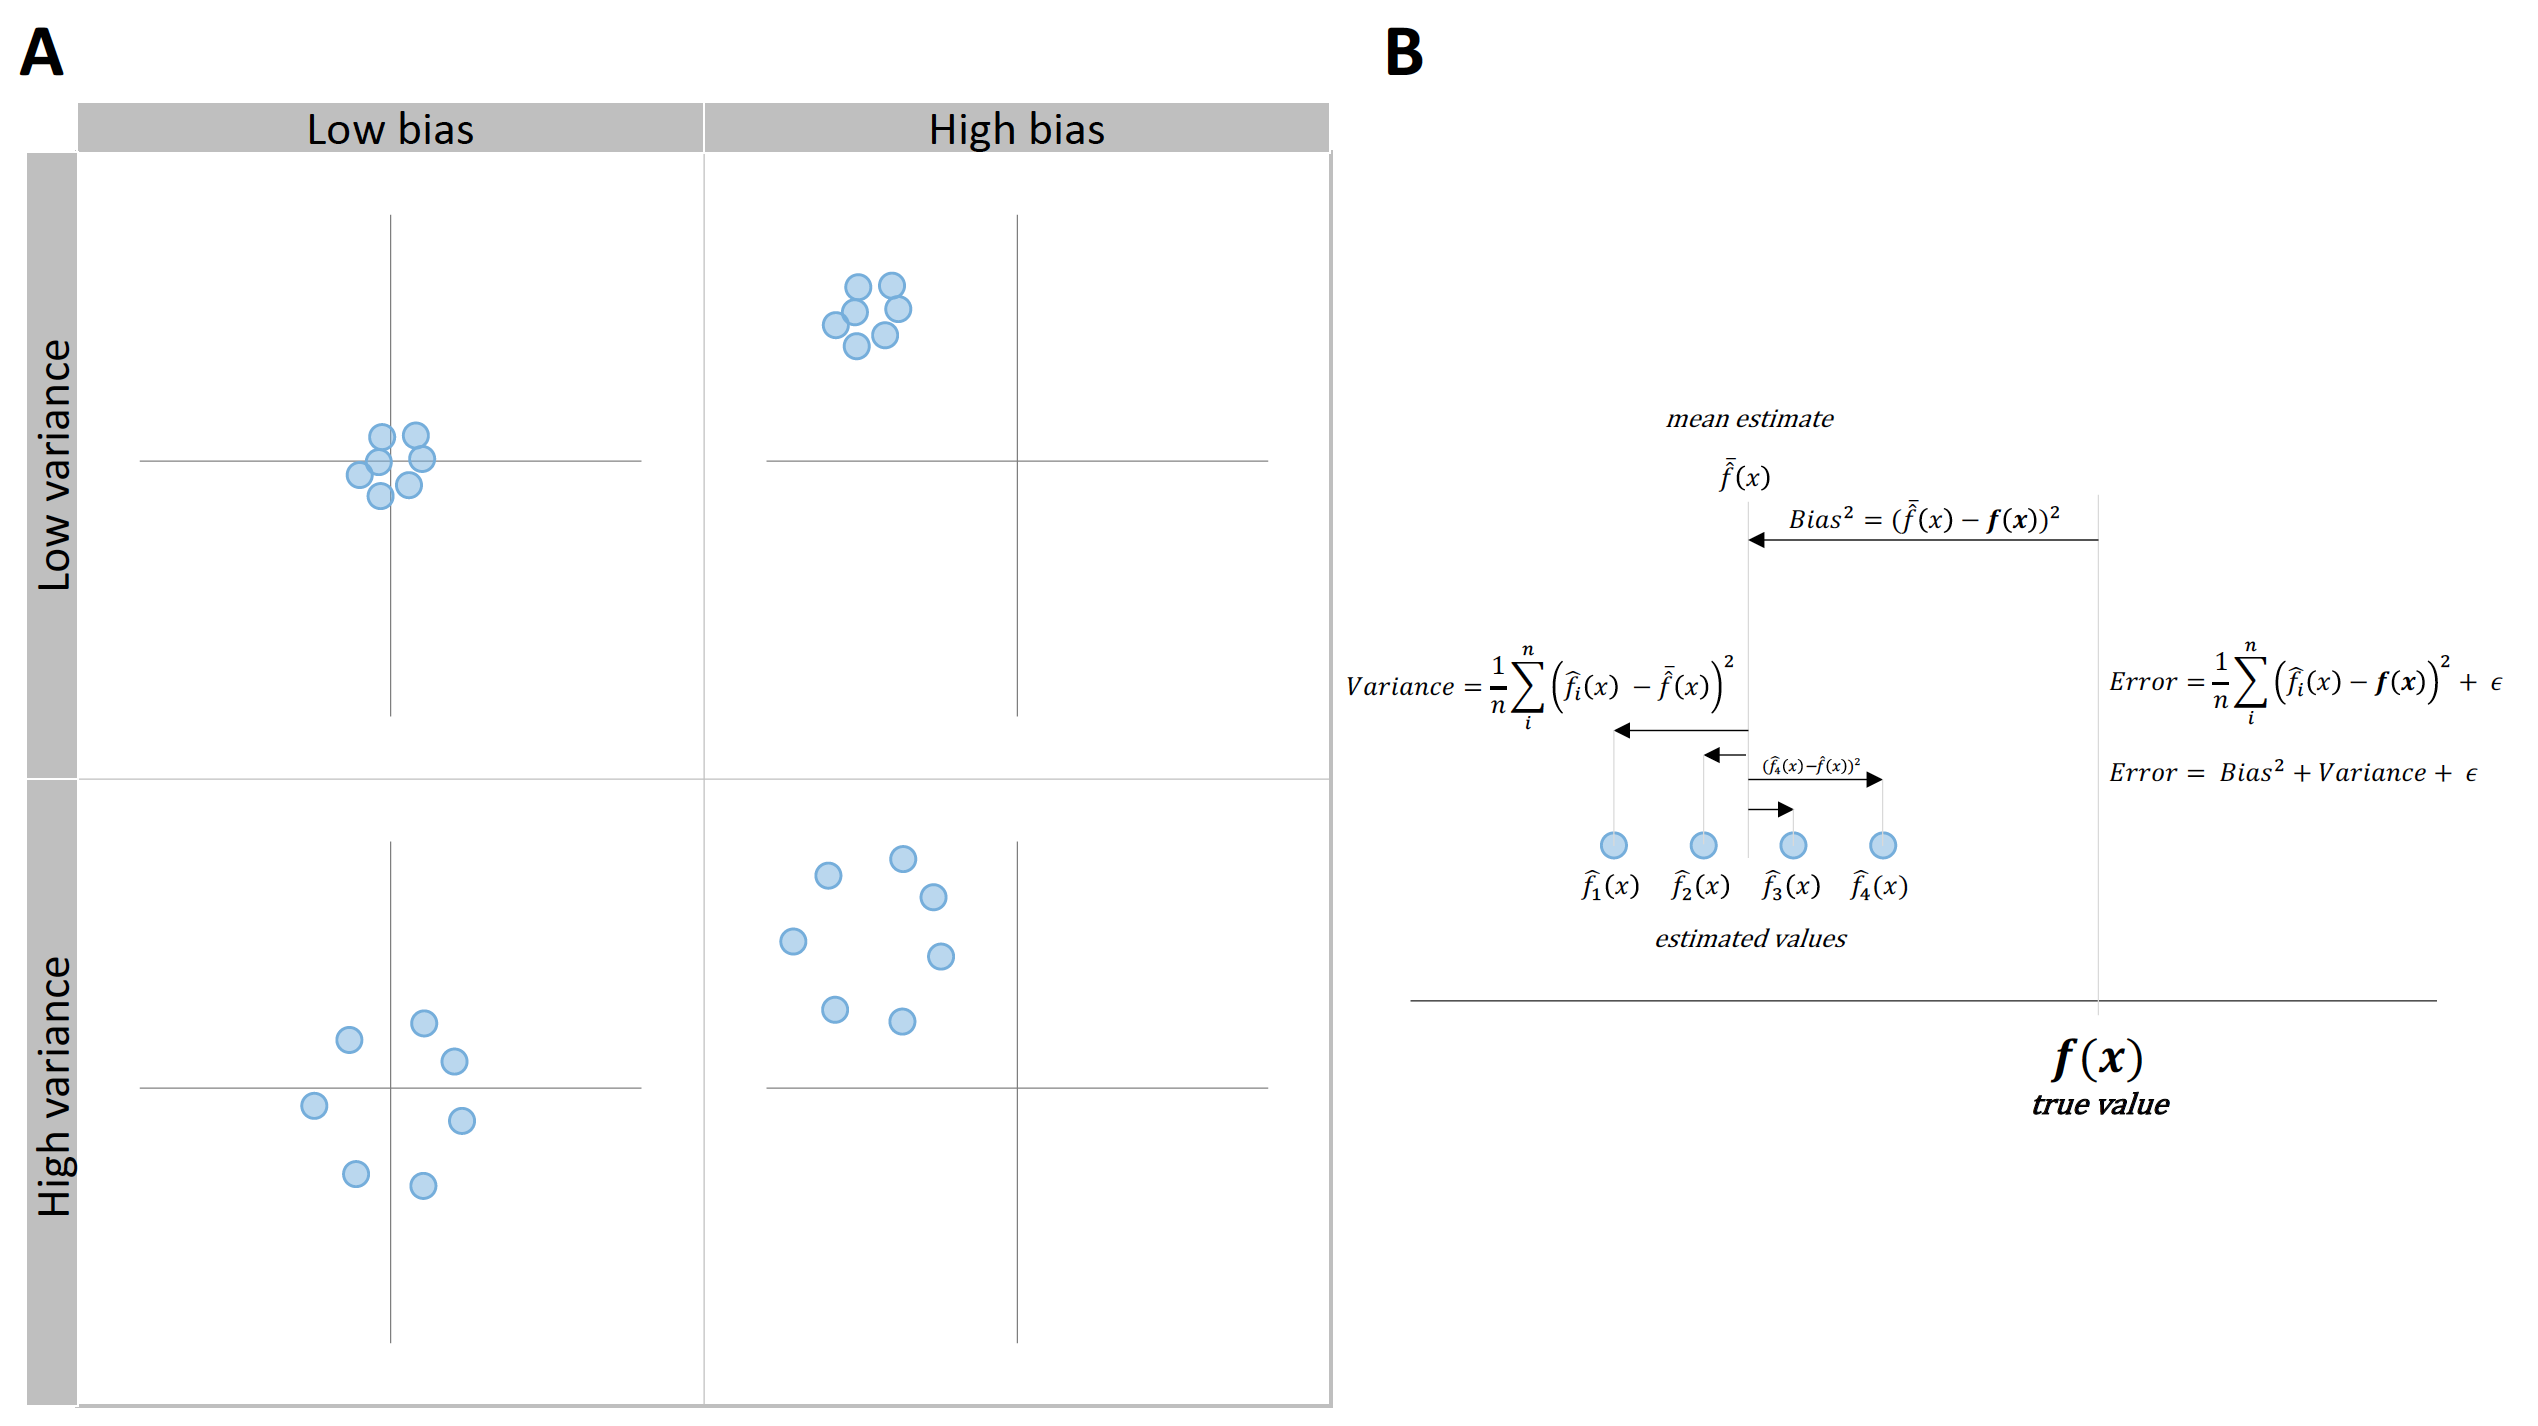
\includegraphics[width=1\linewidth]{figures/bias-variance} 

}

\caption{\textbf{Bias and variance decomposition of the error. A. }Visual representation of \(Bias^2\) and \(Variance\) using the shooting target. \textbf{B.} Error can be decomposed to \(Bias^2\), \(Variance\), and \(Irreducible \: error\), where \(Bias^2\) represents constant or systematic error and \(Variance\) represents variable or random error}\label{fig:bias-variance}
\end{figure}



To understand this concept, we need to run a simulation using \emph{known} relationship between BS and SJ (see Figure \ref{fig:bs-sj-training-testing}, Figure \ref{fig:poly-fit-model}, and Equation \eqref{eq:sj-bs-equation}). Prediction error decomposition to bias and variance is done for a \emph{single} data point. To do that we need to differentiate between the following variables:

\begin{itemize}
\tightlist
\item
  \(x\) predictors. In our case we only have one \(x\) predictor - \(BS\) and we will use \(BS = 1.75\) for this simulation
\item
  \(y_{true}\) value for a particular \(x\) values. In our case \(SJ\) variable represents target variable \(y\), which is equal to \(SJ = 30 + 15\times BS\times\sin(BS)\) or \(SJ=55.83\)cm. Both \(x\) and \(y_{true}\) values are constant across simulations
\item
  \(y_{observed}\) represents observed \(y\) which differs from \(y_{true}\) due stochastic component \(\epsilon\). This implies that \(y_{observed}\) randomly varies across simulations. The equation for \(y_{observed}\) is: \(SJ = 30 + 15\times BS\times\sin(BS) + \mathcal{N}(0,\,2)\). Error \(\epsilon\) represents irreducible error, because it is inherent to DGP and it is equal to \(\mathcal{N}(0,\,2)\).
\item
  \(y_{predicted}\) represents model prediction using the training sample of \(x\) and \(y_{observed}\) values.
\end{itemize}

For every simulation (N=200 simulations in total), the whole sample of N=35 observations is generated from the known DGP. This includes \(x\), \(y_{true}\), and \(y_{observed}\) variables. Polynomial regression models (from 1 to 20 polynomial degrees) are being fitted (or trained) using \(x\) predictors (in our case \(BS\) variable) and \(y_{observed}\) as our target variable. True \(y\) (\(y_{true}\)) is thus unknown to the model, but only to us. After models are trained, we estimate \(y_{predicted}\) using \(BS = 1.75\), for which the \(y_{true}\) is equal to \(SJ=55.83\)cm.

Table \ref{tab:ten-simulations-bias-variance} contains results of the first 10 simulations for 2nd degree polynomial model.



\begin{table}

\caption{\label{tab:ten-simulations-bias-variance}\textbf{Results of first 10 simulations for 2nd degree polynomial linear regression model}}
\centering
\begin{tabular}[t]{rrrrrr}
\toprule
sim & model & x & y\_true & y\_observed & y\_predicted\\
\midrule
1 & 2 & 1.75 & 55.83 & 54.65 & 55.27\\
2 & 2 & 1.75 & 55.83 & 53.80 & 55.34\\
3 & 2 & 1.75 & 55.83 & 56.03 & 55.34\\
4 & 2 & 1.75 & 55.83 & 55.71 & 55.68\\
5 & 2 & 1.75 & 55.83 & 55.52 & 54.91\\
\addlinespace
6 & 2 & 1.75 & 55.83 & 57.55 & 55.81\\
7 & 2 & 1.75 & 55.83 & 52.03 & 55.08\\
8 & 2 & 1.75 & 55.83 & 56.35 & 55.92\\
9 & 2 & 1.75 & 55.83 & 54.05 & 54.64\\
10 & 2 & 1.75 & 55.83 & 58.16 & 55.57\\
\bottomrule
\end{tabular}
\end{table}

To estimate reducible error, \texttt{MSE} estimator is used (Equation \eqref{eq:MSE-reducible-error}.

\begin{equation}
  Reducible \: error = \frac{1}{n_{sim}}\Sigma_{j=1}^{n_{sim}}(y_{predicted_{j,x=1.75}} - y_{true_{x=1.75}})^2
  \label{eq:MSE-reducible-error}
\end{equation}

Reducible error can be decomposed to \(Bias^2\) and \(Variance\), or systematic error and variable or random error. \(Bias^2\) is squared difference between \(y_{true}\) and mean of \(y_{predicted}\) across simulations (Equation \eqref{eq:bias-equation}).

\begin{equation}
  Bias^2 = (\frac{1}{n_{sim}}\Sigma_{j=1}^{n_{sim}}(y_{predicted_{j, x=1.75}}) - y_{true_{x=1.75}})^2
  \label{eq:bias-equation}
\end{equation}

\(Variance\) represents, pretty much, \texttt{SD} of the of the \(y_{predicted}\) and it is an estimate of how much the predictions vary across simulations (Equation \eqref{eq:variance-equation}).

\begin{equation}
  Variance = \frac{1}{n_{sim}}\Sigma_{j=1}^{n_{sim}}(\bar{y_{predicted_{x=1.75}}} - y_{predicted_{j, x=1.75}})^2
  \label{eq:variance-equation}
\end{equation}

Reducible error is thus equal to the sum of \(Bias^2\) and \(Variance\).

If you remember from \protect\hyperlink{description}{Description} section, \(Bias^2\) and \(Variance\) are nothing more than measure of central tendency (i.e.~systematic or constant error) and measure of spread (i.e.~variable or random error). Figure \ref{fig:bias-variance} also illustrates this concept.

Irreducible error is estimated using \texttt{MSE} as well (Equation MSE-irreducible-error).

\begin{equation}
  Irreducible \: error = \frac{1}{n_{sim}}\Sigma_{j=1}^{n_{sim}}(y_{observed_{x=1.75}} - y_{true_{x=1.75}})^2
  \label{eq:MSE-irreducible-error}
\end{equation}

Since we know that the stochastic error in the DGP is normally distributed with SD=2cm, expected irreducible error should be around 4cm (this is because \texttt{MSE} is mean squared error, and \texttt{RMSE}, which is equivalent to \texttt{SD}, is calculated by doing square root of \texttt{MSE}). This might not be exactly 4cm due \emph{sampling error} which is the topic of \protect\hyperlink{statistical-inference}{Statistical inference} section.

As explained in Equation \eqref{eq:reducible-irreducible}, \(Prediction \: error\) is equal to sum of \(Bias^2\), \(Variance\) and \(Irreducible \: error\). Table contains estimated aforementioned errors using all 200 simulations for 2nd degree polynomial linear regression.



\begin{table}

\caption{\label{tab:example-error-decomposition}\textbf{Calculated errors for all 200 simulations for 2nd degree polynomial linear regression}}
\centering
\resizebox{\linewidth}{!}{
\begin{tabular}[t]{rrrrrrr}
\toprule
model & x & y\_true & Prediction error & Bias\textasciicircum{}2 & Variance & Irreducible error\\
\midrule
2 & 1.75 & 55.83 & 5.17 & 0.09 & 0.21 & 4.87\\
\bottomrule
\end{tabular}}
\end{table}

This decomposition of errors is one useful mathematical property when using squared erors that I alluded to in the \protect\hyperlink{cross-validation}{Cross-Validation} section when discussing prediction error metrics.

If we perfrom this analysis for each degree of polynomial fit, we will estimate prediction error, as well as \(Bias^2\) and \(Variance\) across model complexity (i.e.~polynomial degrees). This is visualized in the Figure \ref{fig:bias-variance-simulation}.

\begin{figure}[!htb]

{\centering 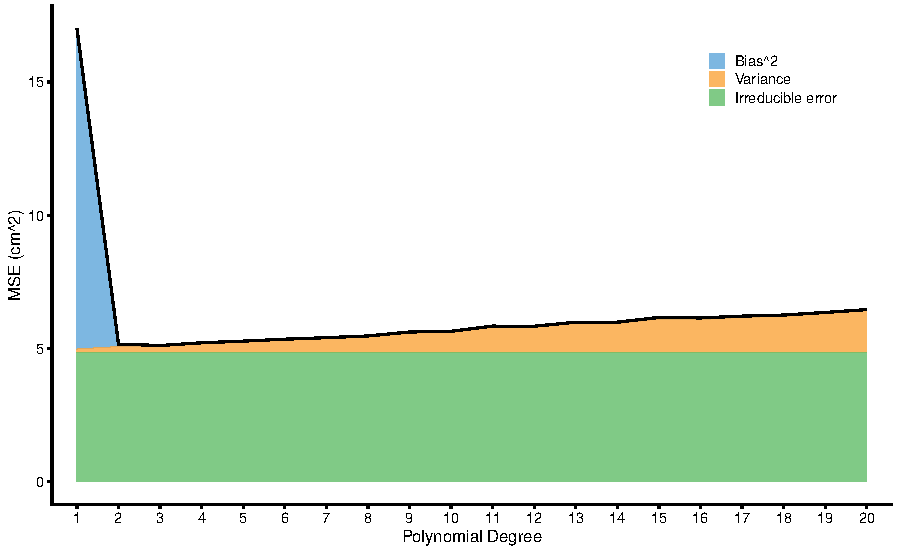
\includegraphics[width=0.9\linewidth]{03-Prediction_files/figure-latex/bias-variance-simulation-1} 

}

\caption{\textbf{Bias and Variance error decomposition. }\(Prediction \: error\) is indicated with the black line, and is decomposed to \(Bias^2\), \(Variance\), and \(Irreducible \: error\). These are represents with areas of different color}\label{fig:bias-variance-simulation}
\end{figure}



Beside decomposition of \(Prediction \: error\) to \(Bias^2\), \(Variance\) and \(Irreducible \: error\), it is important to notice the \emph{trade-off} between \(Bias^2\) and \(Variance\). Linear regression models with lower polynomial degree, particularly 1st degree which is simple linear regression, has higher \(Bias^2\) due imposed \emph{linearity} of the model (we can say that linear regression model is more \emph{biased}). As \(Bias^2\) decreases with more flexible models (i.e.~higher polynomial degree), \(Variance\) increase due model being too \emph{jumpy} across simulations. To achieve best prediction (or the lower \(Prediction \: error\)) a balance between \(Bias^2\) and \(Variance\) needs to be found, both within a particular model and across models. The \emph{free lunch} theorem (Kuhn and Johnson \protect\hyperlink{ref-kuhnAppliedPredictiveModeling2018}{2018}; Yarkoni and Westfall \protect\hyperlink{ref-yarkoniChoosingPredictionExplanation2017}{2017}) states that there is no single model that is the best across all different sets of problems. One needs to evaluate multiple models\footnote{Or to utilize subject matter knowledge needed to select the model. More about this topic can be found in the \protect\hyperlink{subject-matter-knowledge}{Subject matter knowledge} section.} to estimate which one is the best for a particular problem at hand.

To estimate \(Bias^2\) and \(Variance\), \emph{true} DGP must be known. Unfortunately, we do not know these for the real world problems, only for simulations. But even when we do not know \(y_{true}\) values (and thus \(Irreducible \: error\)), concepts of \(Bias^2\) and \(Variance\) can be applied in cross-validation samples (particularly when using multiple repeats) and can estimated using \(y_{observed}\). I will provide one such analysis in \protect\hyperlink{practical-example-mas-and-yoyoir1-prediction}{Practical example: MAS and YoYoIR1 prediction} section.

\hypertarget{interpretability}{%
\section{Interpretability}\label{interpretability}}

As explained, predictive models put predictive performance over explanation of the underlying DGP mechanism (which is treated as a black box). However, sometimes we might be interested in which predictor is the most important, how do predictions change when particular predictor changes, or why\footnote{With the recent laws such as European's DGPR, predictive models needs to be able to explain or provide explanation why particular decision or prediction has been made. Christoph Molnar explains the need for model interpretability with one interesting example: ``By default, machine learning models pick up biases from the training data. This can turn your machine learning models into racists that discriminate against protected groups. Interpretability is a useful debugging tool for detecting bias in machine learning models. It might happen that the machine learning model's, you have trained for, automatic approval or rejection of credit applications discriminates against a minority. Your main goal is to grant loans only to people who will eventually repay them. The incompleteness of the problem formulation in this case lies in the fact that you not only want to minimize loan defaults, but are also obliged not to discriminate on the basis of certain demographics. This is an additional constraint that is part of your problem formulation (granting loans in a low-risk and compliant way) that is not covered by the loss function the machine learning model was optimized for.'' (Molnar \protect\hyperlink{ref-molnarInterpretableMachineLearning2018}{2018}, 11)} model made a particular prediction for a case of interest (Kuhn and Johnson \protect\hyperlink{ref-kuhnAppliedPredictiveModeling2018}{2018}; Molnar \protect\hyperlink{ref-molnarInterpretableMachineLearning2018}{2018}; Ribeiro, Singh, and Guestrin \protect\hyperlink{ref-ribeiroWhyShouldTrust2016}{2016}). Model interpretability can be defined as the degree to which a human can understand the cause of a decision (Miller \protect\hyperlink{ref-millerExplanationArtificialIntelligence2017}{2017}; Molnar \protect\hyperlink{ref-molnarInterpretableMachineLearning2018}{2018}; Biecek and Burzykowski \protect\hyperlink{ref-biecekPredictiveModelsExplore2019}{2019}). Some models are more inherently interpretable (e.g.~linear regression) and some are indeed very complex and hard to interpret (e.g.~random forest or neural networks). For this reason, there are \emph{model-agnostic} techniques that can help increase model interpretability.

Excellent book and R (R Core Team \protect\hyperlink{ref-R-base}{2020}) package by Christoph Molnar (Molnar, Bischl, and Casalicchio \protect\hyperlink{ref-molnarImlPackageInterpretable2018}{2018}; Molnar \protect\hyperlink{ref-molnarInterpretableMachineLearning2018}{2018}) demonstrates a few model-agnostic interpretation techniques. One such technique is estimating which predictor is the most important (\emph{variable importance}). One method for estimating variable importance involves \emph{perturbing} one predictor and estimating the change in model performance. The predictor whose perturbing causes the biggest change in model performance can be considered the most important (Kuhn and Johnson \protect\hyperlink{ref-kuhnAppliedPredictiveModeling2018}{2018}; Molnar \protect\hyperlink{ref-molnarInterpretableMachineLearning2018}{2018}). There are others approaches for estimating variable importance (B. M. Greenwell \protect\hyperlink{ref-RJ-2017-016}{2017}\protect\hyperlink{ref-RJ-2017-016}{b}). Those interested in further details can also check \emph{vip} (Greenwell, Boehmke, and Gray \protect\hyperlink{ref-R-vip}{2020}) R (R Core Team \protect\hyperlink{ref-R-base}{2020}) package.

One might be interested in how the predicted outcome changes when particular predictor changes. Techniques such as \emph{partial dependence plot} (PDP), \emph{individual conditional expectation} (ICE) and \emph{accumulated local effects} (ALE) can be helpful in interpreting the effect of particular predictor on predicted outcome (Molnar, Bischl, and Casalicchio \protect\hyperlink{ref-molnarImlPackageInterpretable2018}{2018}; Molnar \protect\hyperlink{ref-molnarInterpretableMachineLearning2018}{2018}; Goldstein et al. \protect\hyperlink{ref-goldsteinPeekingBlackBox2013}{2013}; Zhao and Hastie \protect\hyperlink{ref-zhaoCausalInterpretationsBlackBox2019}{2019}; B. M. Greenwell \protect\hyperlink{ref-R-pdp}{2017}\protect\hyperlink{ref-R-pdp}{a}). Similar techniques are utilized in \protect\hyperlink{prediction-as-a-complement-to-causal-inference}{Prediction as a complement to causal inference} section. Interested readers are also directed toward \emph{visreg} (Breheny and Burchett \protect\hyperlink{ref-R-visreg}{2017}) and \emph{effects} (Fox and Weisberg \protect\hyperlink{ref-R-effects_a}{2018}; Fox \protect\hyperlink{ref-R-effects_b}{2003}; Fox and Hong \protect\hyperlink{ref-R-effects_c}{2009}) R (R Core Team \protect\hyperlink{ref-R-base}{2020}) packages for more information about visualizing models.

It is important to keep in mind that these model-agnostic explanations should not be automatically treated as causal explanations (Pearl and Mackenzie \protect\hyperlink{ref-pearlBookWhyNew2018}{2018}; Pearl \protect\hyperlink{ref-pearlSevenToolsCausal2019}{2019}), but as mere association and descriptive analysis that can still be useful in understanding and interpreting the underlying predictive \emph{black-box}. They are not without problems, such as correlated variables, interactions and other issues (Altmann et al. \protect\hyperlink{ref-altmannLimitationsInterpretableMachine2019}{2019}).

According to Judea Pearl (Pearl and Mackenzie \protect\hyperlink{ref-pearlBookWhyNew2018}{2018}; Pearl \protect\hyperlink{ref-pearlSevenToolsCausal2019}{2019}), prediction models should belong to the first level of \emph{ladder of causation}\footnote{``Pearl's causal meta-model involves a three-level abstraction he calls the ladder of causation. The lowest level, \emph{Association} (seeing/observing), entails the sensing of regularities or patterns in the input data, expressed as correlations. The middle level, \emph{Intervention} (doing), predicts the effects of deliberate actions, expressed as causal relationships. The highest level, \emph{Counterfactuals} (imagining), involves constructing a theory of (part of) the world that explains why specific actions have specific effects and what happens in the absence of such actions'' (Wikipedia contributors \protect\hyperlink{ref-wiki:xxx}{2019})}, which represents simple ``curve fitting''. Although in under special conditions these techniques can have causal interpretation (Zhao and Hastie \protect\hyperlink{ref-zhaoCausalInterpretationsBlackBox2019}{2019}).

The distinctions, similarities and issues between predictive modeling, machine learning and causal inference is currently hot topic in debates between machine learning specialists, statisticians and philosophers of science and it is beyond the scope of this book to delve into the debate. Interested readers are directed towards work by Miguel Hernan (Hernán \protect\hyperlink{ref-hernanCausalDiagramsDraw2017}{2017}, \protect\hyperlink{ref-hernanDoesWaterKill2016}{2016}, \protect\hyperlink{ref-hernanCWordScientificEuphemisms2018}{2018}; Hernán and Robins, \protect\hyperlink{ref-hernanCausalInference2019}{n.d.}; Hernán, Hsu, and Healy \protect\hyperlink{ref-hernanSecondChanceGet2019}{2019}), Judea Pearl (Pearl and Mackenzie \protect\hyperlink{ref-pearlBookWhyNew2018}{2018}; Pearl, Glymour, and Jewell \protect\hyperlink{ref-pearlCausalInferenceStatistics2016}{2016}; Pearl \protect\hyperlink{ref-pearlSevenToolsCausal2019}{2019}, \protect\hyperlink{ref-pearlCausalInferenceStatistics2009}{2009}), Samantha Kleinberg (Kleinberg \protect\hyperlink{ref-kleinbergWhyGuideFinding2015}{2015}, \protect\hyperlink{ref-kleinbergCausalityProbabilityTime2018}{2018}) and others (Watts et al. \protect\hyperlink{ref-wattsExplanationPredictionCausality2018}{2018}; Saddiki and Balzer \protect\hyperlink{ref-saddikiPrimerCausalityData2018}{2018}; Kleinberg, Liang, and Mullainathan \protect\hyperlink{ref-kleinbergTheoryPredictiveIt2017}{2017}; Breiman \protect\hyperlink{ref-breimanStatisticalModelingTwo2001}{2001}; Shmueli \protect\hyperlink{ref-shmueliExplainPredict2010}{2010}; Yarkoni and Westfall \protect\hyperlink{ref-yarkoniChoosingPredictionExplanation2017}{2017}). The next \protect\hyperlink{causal-inference}{Causal Inference} section introduces the causal inference as a specific task of statistical modeling.

\hypertarget{magnitude-based-prediction-estimators}{%
\section{Magnitude-based prediction estimators}\label{magnitude-based-prediction-estimators}}

Similar to the magnitude-based estimators from \protect\hyperlink{describing-relationship-between-two-variables}{Describing relationship between two variables} section, one can utilize target variable SESOI to get magnitude-based estimates of predictive performance of the model. Rather than utilizing RSE as an estimate of the model fit in the training data, one can utilize \emph{cross-validated RMSE} (\texttt{cvRMSE}), \texttt{SESOI\ to\ cvRMSE}, as well as \emph{cross-validated proportion of practically equivalent residuals} (\texttt{cvPPER}) estimators.

Continuing with the squat jump height and relative squat 1RM example, one can assume that the SESOI in the squat jump is ±1cm. For the sake of example, we can \emph{feature engineer} (Kuhn and Johnson \protect\hyperlink{ref-kuhnAppliedPredictiveModeling2018}{2018}, \protect\hyperlink{ref-kuhnFeatureEngineeringSelection2019}{2019}) relative squat 1RM variable to include all 20 degree polynomials. This way, we have created 20 predictor variables. To avoid overfitting, \emph{elastic-net model} (Friedman, Hastie, and Tibshirani \protect\hyperlink{ref-friedmanRegularizationPathsGeneralized2010}{2010}) implemented in the \emph{caret} R package (Kuhn and Johnson \protect\hyperlink{ref-kuhnAppliedPredictiveModeling2018}{2018}; Kuhn et al. \protect\hyperlink{ref-kuhnCaretClassificationRegression2018}{2018}) is utilized, as well as repeated cross-validation involving 3 splits repeated 10 times. Predictive model performance is evaluated by using \texttt{cvRMSE}, together with magnitude-based performance estimators (\texttt{SESOI\ to\ cvRMSE} and \texttt{cvPPER}).

Elastic-net model represents regression method that linearly combines the \emph{L1} and \emph{L2} penalties of the lasso and ridge methods, or \emph{alpha} and \emph{lambda} tuning parameters (Friedman, Hastie, and Tibshirani \protect\hyperlink{ref-friedmanRegularizationPathsGeneralized2010}{2010}; James et al. \protect\hyperlink{ref-jamesIntroductionStatisticalLearning2017}{2017}; Kuhn and Johnson \protect\hyperlink{ref-kuhnAppliedPredictiveModeling2018}{2018}). Total of nine combinations of tuning parameters is evaluated using aforementioned repeated cross-validation, and the model with minimal \texttt{cvRMSE} is selected as the best one. Performance metrics of the best model are further reported. Table \ref{tab:predictive-metrics-mag-based} contains cross-validated best model performance metrics together with model performance on the training data set.



\begin{table}

\caption{\label{tab:predictive-metrics-mag-based}\textbf{Common predictive metrics and magnitude-based predictive metrics. }Metrics starting with \textbf{cv} indicate cross-validated performance metrics. Metrics without \textbf{cv} indicate performance metrics on the training data set, which is often more optimistic}
\centering
\resizebox{\linewidth}{!}{
\begin{tabular}[t]{lrrrrrr}
\toprule
SESOI (cm) & cvRMSE (cm) & SESOI to cvRMSE & cvPPER & RMSE (cm) & SESOI to RMSE & PPER\\
\midrule
±1 & 2.19 & 0.91 & 0.33 & 1.99 & 1.01 & 0.38\\
\bottomrule
\end{tabular}}
\end{table}

Utilizing \emph{apriori} known SESOI gives us practical \emph{anchor} to evaluate predictive model performance. Reported \texttt{SESOI\ to\ cvRMSE} (0.91) as well as \texttt{cvPPER} (0.33) indicate very poor predictive performance of the model. In practical terms, utilizing relative squat 1RM doesn't produce practically meaningful predictions given SESOI of ±1cm and the model as well as the data sample utilized.

Model performance can be visualized using the training data set (Figure \ref{fig:elastic-net-prediction}). \texttt{PPER} estimator, for both cross-validate estimate and training data performance estimate, utilized \texttt{SD} of the residuals and provided SESOI. Grey band on panels A and B on Figure \ref{fig:elastic-net-prediction} represents SESOI, and as can be visually inspected, model residuals are much wider than the SESOI, indicating poor practical predictive performance.

\begin{figure}[!htb]

{\centering 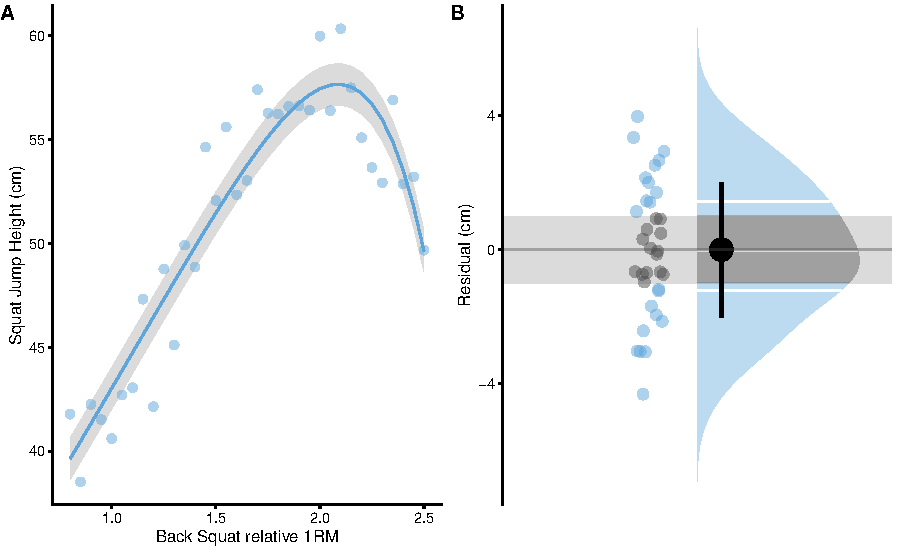
\includegraphics[width=0.9\linewidth]{03-Prediction_files/figure-latex/elastic-net-prediction-1} 

}

\caption{\textbf{Model performance on the training data set. A. }Model with the lowest \texttt{cvRMSE} is selected. SESOI is depicted as grey band around the model prediction (blue line). \textbf{B.} Residuals scatter plot. Residuals outside of the SESOI band (grey band) indicate prediction which error is practically significant. \texttt{PPER} represents proportion of residuals inside the SESOI band}\label{fig:elastic-net-prediction}
\end{figure}



Predictive tasks are focusing on providing the best predictions on the novel or unseen data without much concern about the underlying DGP. Predictive model performance can be evaluated by using magnitude-based approach to give insights into practical significance of the predictions. These magnitude-based prediction estimators, can be used to complement explanatory or causal inference tasks, rather than relying solely on the group-based and average-based estimators. This topic is further discussed in the \protect\hyperlink{prediction-as-a-complement-to-causal-inference}{Prediction as a complement to causal inference} section.

\hypertarget{practical-example-mas-and-yoyoir1-prediction}{%
\section{Practical example: MAS and YoYoIR1 prediction}\label{practical-example-mas-and-yoyoir1-prediction}}

In \protect\hyperlink{describing-relationship-between-two-variables}{Describing relationship between two variables} we have used two physical performance tests, MAS and YoYoIR1, to showcase relationship or association between two variables. Besides mere association, we have stepped into the domain of prediction by utilizing magnitude-based estimators such as \texttt{PPER} and \texttt{SESOI\ to\ RMSE}. As you have learned so far in this section, these predictions were made on the training data set. Let's implement concepts learned so far to estimate predictive performance on the unseen data. Why is this important? Although very simple model, we are interested in predicting MAS from YoYoIR1 test score for a new or unseen individual. For this reason, it is important to get estimates of model performance on the unseen athletes.

\hypertarget{predicting-mas-from-yoyoir1}{%
\subsection{Predicting MAS from YoYoIR1}\label{predicting-mas-from-yoyoir1}}

Let's first estimate predictive performance when predicting MAS scores from the YoYoIR1 score using MAS SESOI ±0.5km/h and linear regression.

Figure \ref{fig:mas-yoyo-ba} consists of two panels. Panel A depicts scatter plot between YoYoIR1 and MAS scores (black line represents linear model fit). Panel B depicts \(y_{predicted}\) (predicted or fitted MAS using simple linear regression; i.e.~the black line on the panel A) against the model residuals \(y_residual = y_{predicted} - y_{observed}\), or Predicted MAS - MAS. The data points represent model performance on the full training data set.

\begin{figure}[!htb]

{\centering 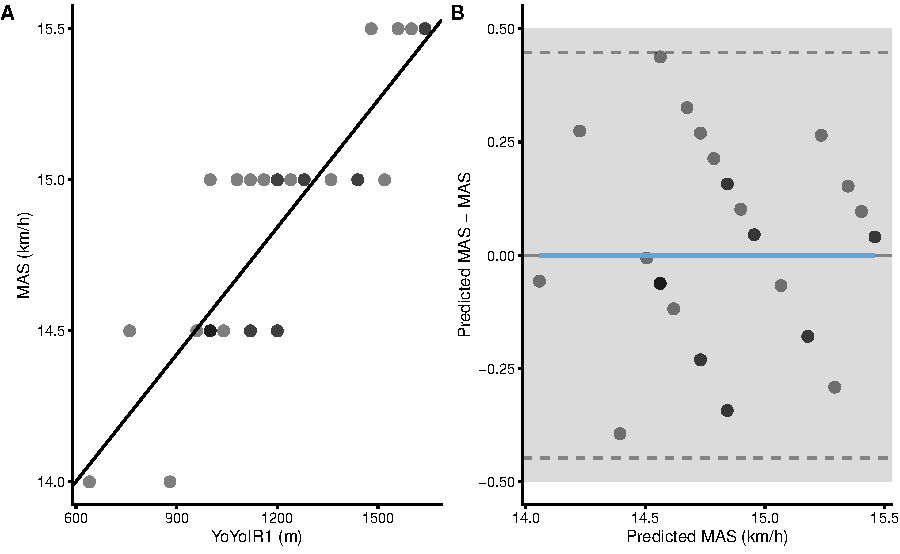
\includegraphics[width=0.9\linewidth]{03-Prediction_files/figure-latex/mas-yoyo-ba-1} 

}

\caption{\textbf{Scatter plot for simple linear regression between MAS and YoYoIR1 using the full training data sample. A. } Scatter plot between MAS and YoYoIR1 scores. Black line indicates model prediction. \textbf{B.} Scatter plot between \(y_{predicted}\) (fitted or predicted MAS) against model residual \(y_{residual} = y_{predicted} - y_{observed}\), or Predicted MAS - MAS. Dotted lines indicate \emph{Levels of Agreement} (LOA; i.e.~upper and lower threshold that contain 95\% of residuals distribution) and grey band indicates SESOI. Blue line indicate linear regression fit of the residuals and is used to indicate issues with the model (residuals)}\label{fig:mas-yoyo-ba}
\end{figure}



Predictive performance for the full training data set is enlisted in the Table \ref{tab:mas-yoyo-training-performance}.



\begin{table}

\caption{\label{tab:mas-yoyo-training-performance}\textbf{Predictive performance using the full training data set}}
\centering
\resizebox{\linewidth}{!}{
\begin{tabular}[t]{rrrrrrrrr}
\toprule
MBE & MAE & RMSE & PPER & SESOI.to.RMSE & R.squared & MinErr & MaxErr & MaxAbsErr\\
\midrule
0 & 0.17 & 0.21 & 0.97 & 4.73 & 0.74 & -0.44 & 0.39 & 0.44\\
\bottomrule
\end{tabular}}
\end{table}

But as already explained, these are not predictive performance estimators for the unseen data. To estimate how the model performs on the unseen data (i.e.~unseen athletes in this case), cross-validation is performed using 3 folds and 5 repeats. Estimated predictive performance for every cross-validation sample is enlisted in the Table \ref{tab:mas-yoyo-cv-performance}.



\begin{table}

\caption{\label{tab:mas-yoyo-cv-performance}\textbf{Predictive performance for every repeated cross-validated sample}}
\centering
\resizebox{\linewidth}{!}{
\begin{tabular}[t]{llrrrrrrrrr}
\toprule
  & fold & MBE & MAE & RMSE & PPER & SESOI to RMSE & R-squared & MinErr & MaxErr & MaxAbsErr\\
\midrule
1 & Fold1.Rep1 & -0.13 & 0.27 & 0.29 & 0.87 & 3.42 & 0.62 & -0.46 & 0.38 & 0.46\\
2 & Fold1.Rep2 & -0.04 & 0.13 & 0.14 & 0.99 & 7.15 & 0.87 & -0.22 & 0.15 & 0.22\\
3 & Fold1.Rep3 & 0.13 & 0.24 & 0.27 & 0.90 & 3.74 & 0.79 & -0.27 & 0.49 & 0.49\\
4 & Fold1.Rep4 & -0.17 & 0.25 & 0.28 & 0.89 & 3.52 & 0.41 & -0.51 & 0.26 & 0.51\\
5 & Fold1.Rep5 & 0.08 & 0.20 & 0.24 & 0.92 & 4.20 & 0.77 & -0.28 & 0.46 & 0.46\\
\addlinespace
6 & Fold2.Rep1 & 0.09 & 0.15 & 0.19 & 0.97 & 5.18 & 0.87 & -0.27 & 0.37 & 0.37\\
7 & Fold2.Rep2 & 0.05 & 0.20 & 0.24 & 0.93 & 4.16 & 0.71 & -0.31 & 0.41 & 0.41\\
8 & Fold2.Rep3 & -0.14 & 0.18 & 0.22 & 0.96 & 4.65 & 0.81 & -0.38 & 0.18 & 0.38\\
9 & Fold2.Rep4 & -0.02 & 0.13 & 0.17 & 0.98 & 5.92 & 0.75 & -0.30 & 0.33 & 0.33\\
10 & Fold2.Rep5 & -0.07 & 0.21 & 0.27 & 0.89 & 3.76 & 0.27 & -0.50 & 0.33 & 0.50\\
\addlinespace
11 & Fold3.Rep1 & 0.04 & 0.13 & 0.16 & 0.99 & 6.27 & 0.60 & -0.20 & 0.31 & 0.31\\
12 & Fold3.Rep2 & -0.01 & 0.20 & 0.24 & 0.92 & 4.21 & 0.54 & -0.45 & 0.34 & 0.45\\
13 & Fold3.Rep3 & 0.02 & 0.15 & 0.21 & 0.95 & 4.74 & 0.51 & -0.44 & 0.35 & 0.44\\
14 & Fold3.Rep4 & 0.21 & 0.23 & 0.28 & 0.91 & 3.57 & 0.83 & -0.06 & 0.53 & 0.53\\
15 & Fold3.Rep5 & -0.01 & 0.17 & 0.19 & 0.97 & 5.29 & 0.82 & -0.32 & 0.34 & 0.34\\
\bottomrule
\end{tabular}}
\end{table}

As explained in \protect\hyperlink{cross-validation}{Cross-Validation} section, to calculate overall cross-validated performance, the \texttt{mean} is calculated for the performance metrics in the Table \ref{tab:mas-yoyo-cv-performance}. Besides reporting the \texttt{mean} as the summary for predictive performances across cross-validated samples, \texttt{SD}, \texttt{min}, and \texttt{max} can be reported too. Another method of summarizing predictive performance over cross-validated samples would be to \emph{bind} or \emph{pool} all \(y_{observed}\) and \(y_{predicted}\) scores from the test samples together and then calculate \emph{overall} predictive performance metrics. These pooled cross\_validated \(y_{observed}\) and \(y_{predicted}\) can also be visualized using the residuals plot (Panel C in Figure \ref{fig:mas-yoyo-ba-cross-validated}).

\begin{figure}[!htb]

{\centering 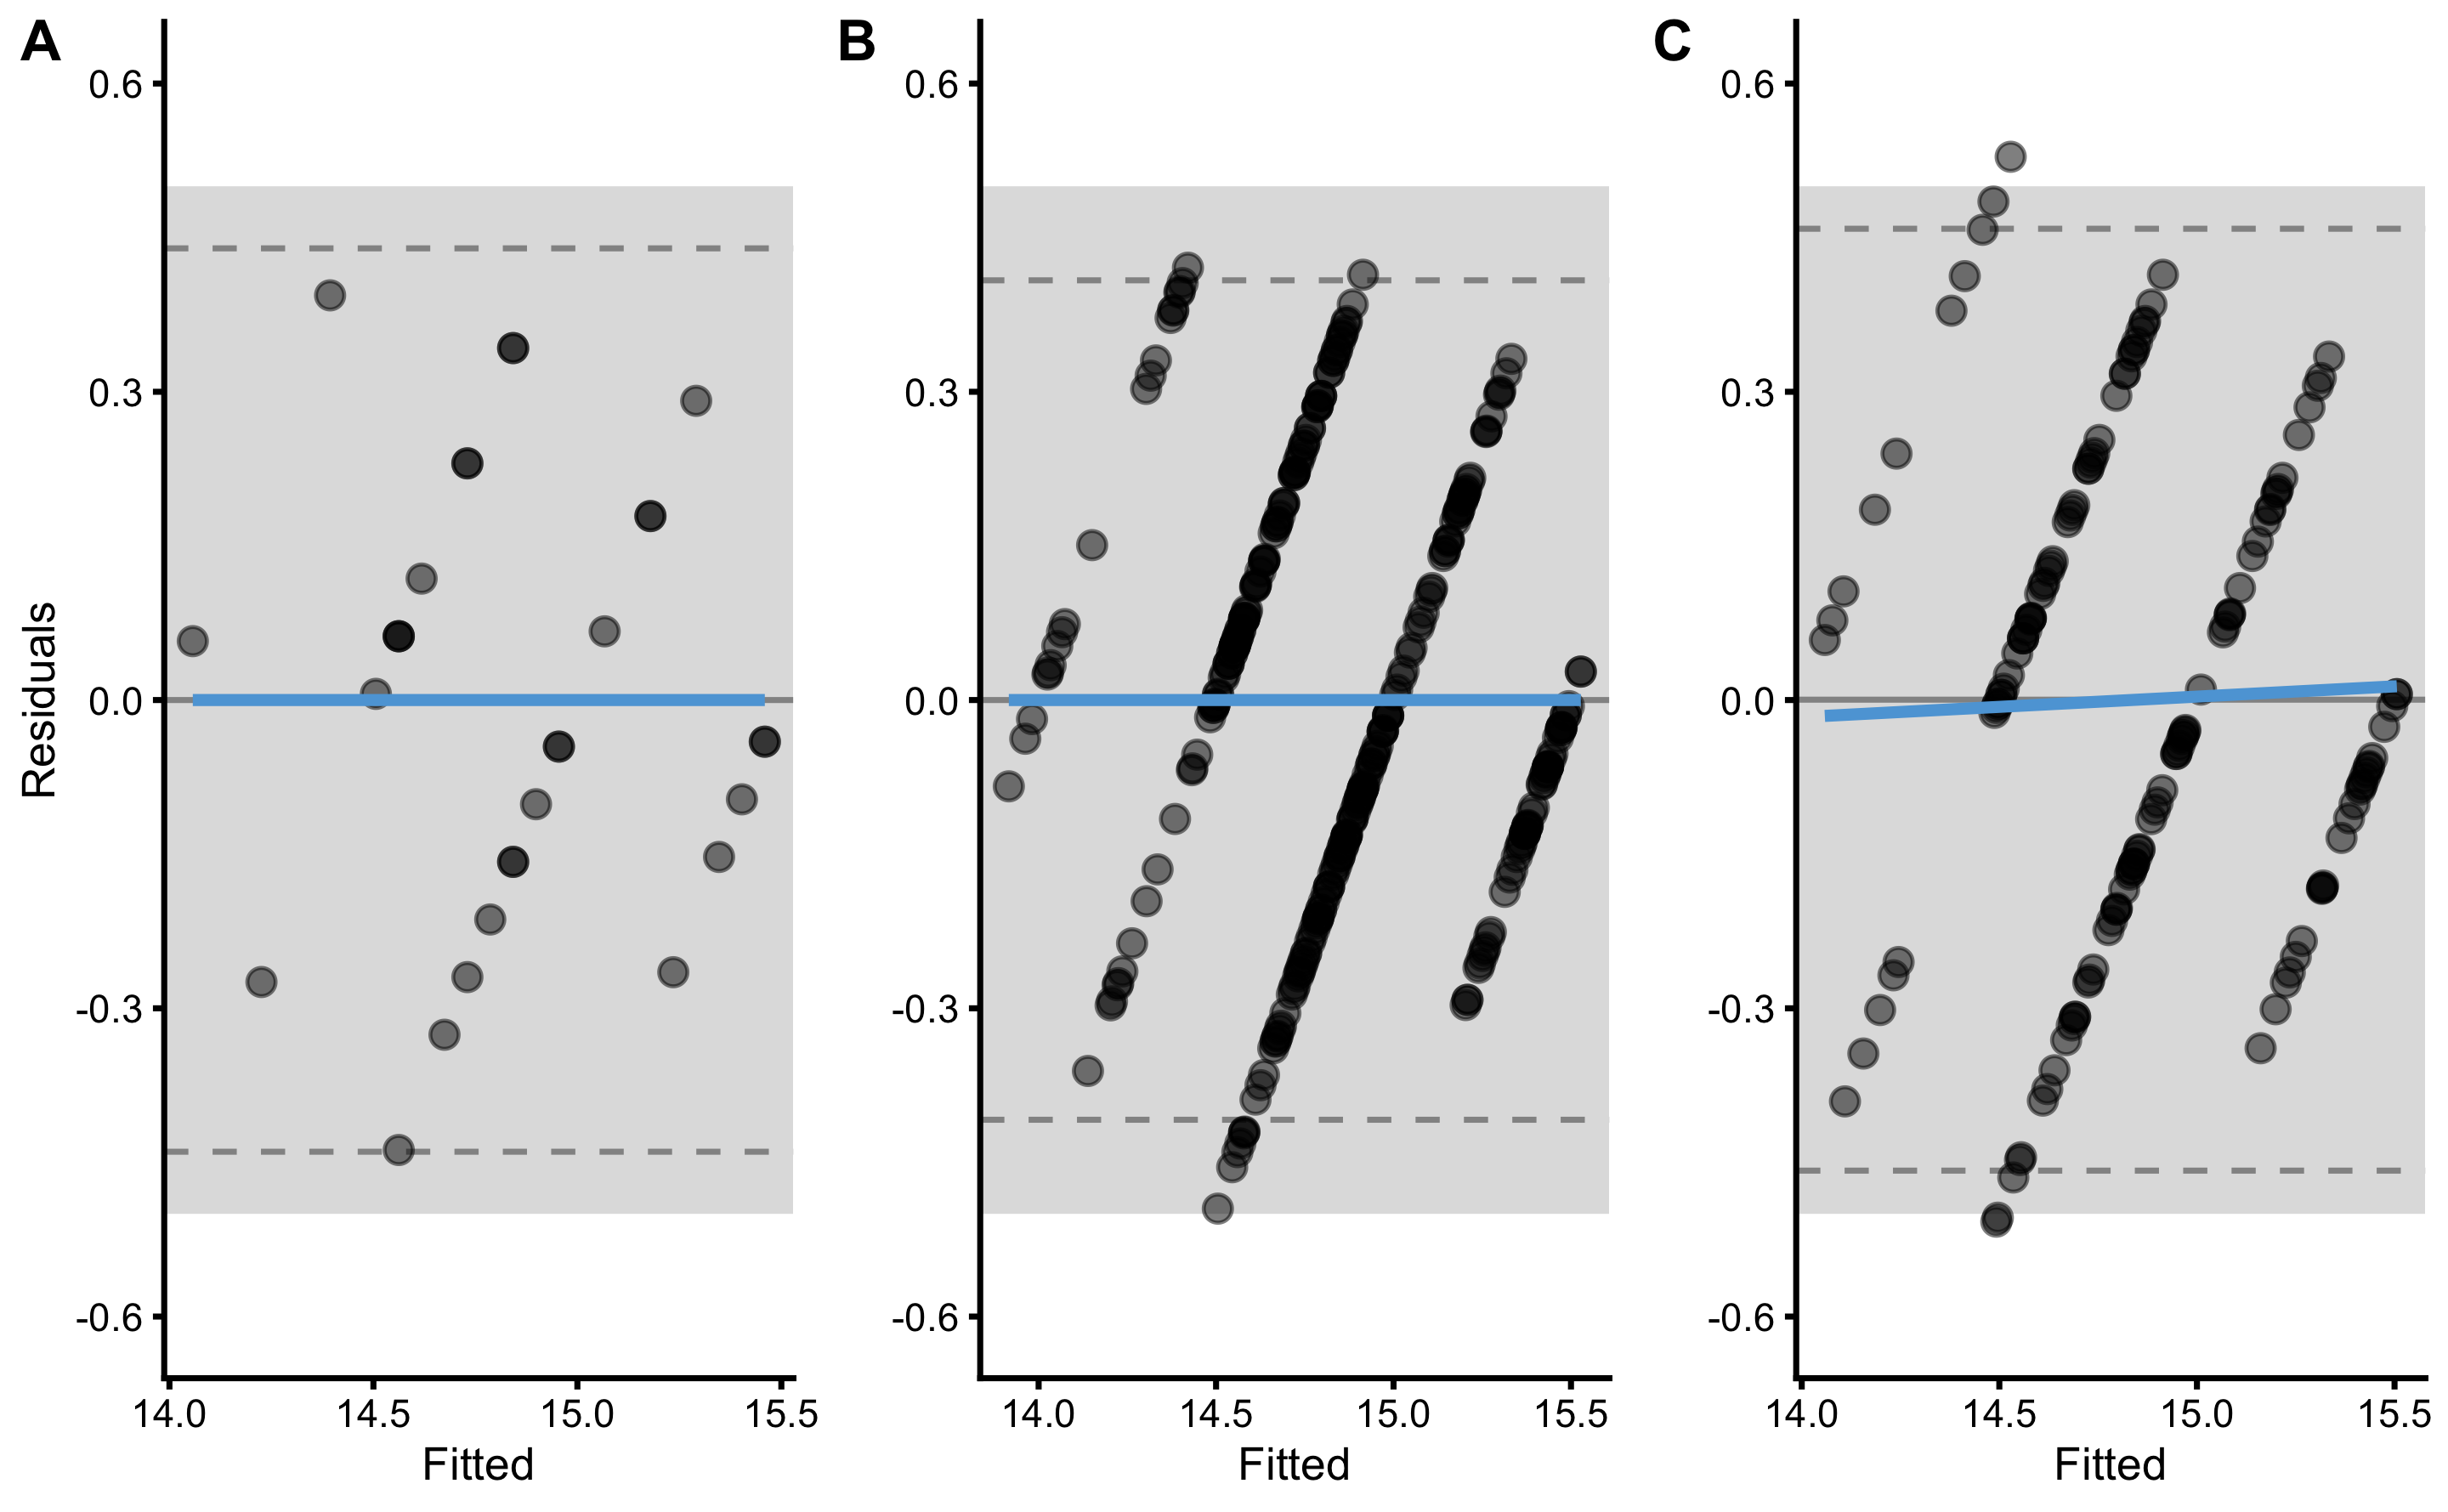
\includegraphics[width=0.9\linewidth]{03-Prediction_files/figure-latex/mas-yoyo-ba-cross-validated-1} 

}

\caption{\textbf{Residuals plot. A. } Model residuals using the training data. This is exactly the same as panel B in Figure \ref{fig:mas-yoyo-ba}. \textbf{B.} Model residuals using the cross-validated training data. \textbf{C.} Model residuals using the cross-validated testing data.}\label{fig:mas-yoyo-ba-cross-validated}
\end{figure}



As can be seen from the panels B and C in Figure \ref{fig:mas-yoyo-ba-cross-validated}, since we have used 5 repeats of the 3-fold cross-validations, each \(y_{observed}\) will have 5 assigned \(y_{predicted}\) scores. These can be used to estimate \(Bias^2\) and \(Variance\) as explained in the \protect\hyperlink{bias-variance-decomposition-and-trade-off}{Bias-Variance decomposition and trade-off} section. Since we do not know the \(y_{true}\) scores, we can only estimate \(Bias^2\) and \(Variance\) of the model for each \(y_{observed}\) using cross-validated \(y_{predicted}\). This is, of course, only possible if multiple repeats of cross-validation are performed. It bears repeating that this \(Bias^2\) and \(Variance\) decomposition of the prediction error using cross-validated \(y_{predicted}\) and \(y_{observed}\) are \textbf{NOT} the same as when using simulation and known DGP as done in \protect\hyperlink{bias-variance-decomposition-and-trade-off}{Bias-Variance decomposition and trade-off} section.

But these can be useful diagnostic tools for checking where the model fails (e.g.~what particular observation might be problematic or outlier, as well how does \(Bias^2\) and \(Variance\) changes across \(y_{observed}\) continuum). These two concepts are depicted on Figure \ref{fig:mas-yoyo-bias-variance-index} and Figure \ref{fig:mas-yoyo-bias-variance-y-obs}.

\begin{figure}[!htb]

{\centering 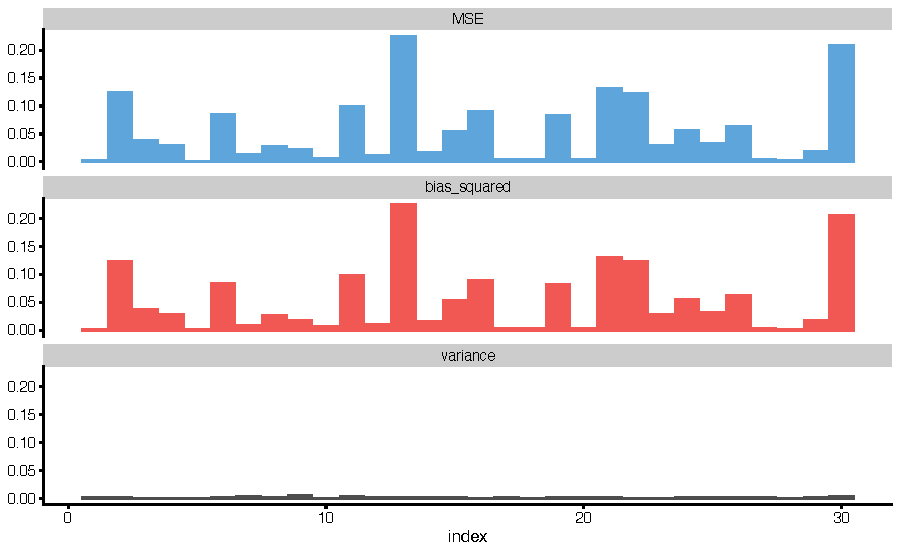
\includegraphics[width=0.9\linewidth]{03-Prediction_files/figure-latex/mas-yoyo-bias-variance-index-1} 

}

\caption{\textbf{Prediction error (\(MSE\)), \(Bias^2\), and \(Variance\) across repeated cross-validated testing data. }X-axis on the panels represents observation \emph{index}, as in \(y_{i, observed}\)}\label{fig:mas-yoyo-bias-variance-index}
\end{figure}



\begin{figure}[!htb]

{\centering 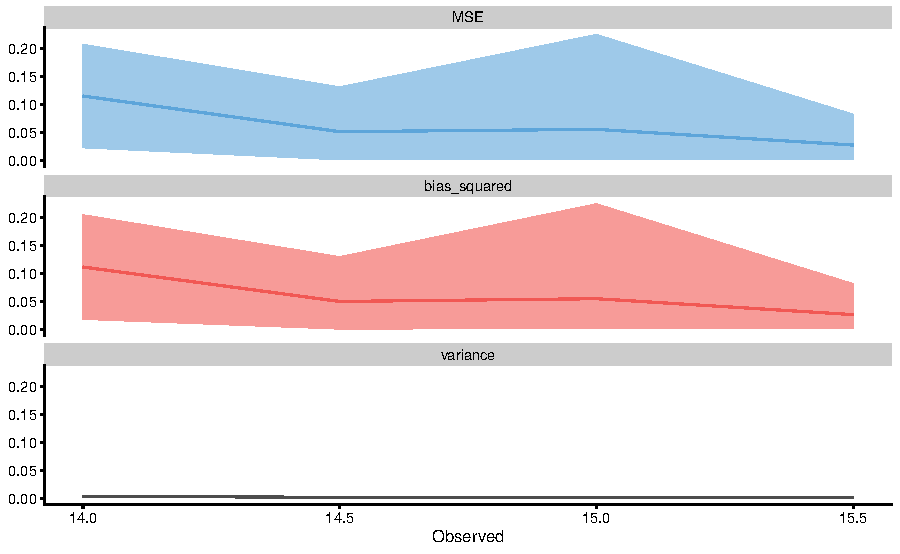
\includegraphics[width=0.9\linewidth]{03-Prediction_files/figure-latex/mas-yoyo-bias-variance-y-obs-1} 

}

\caption{\textbf{Prediction error (\(MSE\)), \(Bias^2\) and \(Variance\) across repeated cross-validated testing data. }X-axis on the panels represent \(y_{observed}\). Since there might be multiple equal \(y_{observed}\), \texttt{min} and \texttt{max} are used and represent \emph{ribbon} over \texttt{mean} (indicated by line)}\label{fig:mas-yoyo-bias-variance-y-obs}
\end{figure}



Since \(Bias\) and \(Variance\) represent a quantitative summary of the residuals across cross-validations, the residuals and predicted observations across cross-validation testing folds can be visualized in more details as depicted on Figures \ref{fig:mas-yoyo-bias-cv-prediction-index} and \ref{fig:mas-yoyo-bias-cv-prediction-observation}.

\begin{figure}[!htb]

{\centering 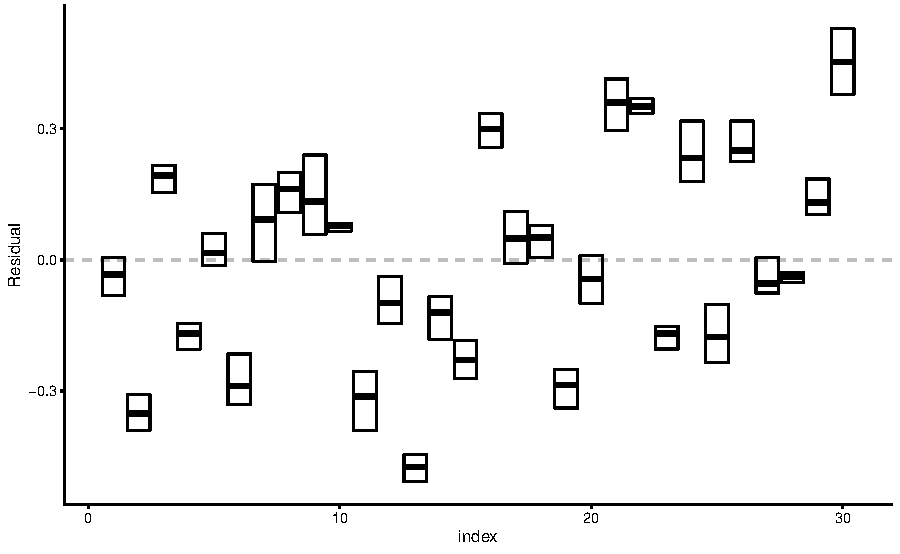
\includegraphics[width=0.9\linewidth]{03-Prediction_files/figure-latex/mas-yoyo-bias-cv-prediction-index-1} 

}

\caption{\textbf{Testing prediction residuals across cross-validation folds summarized with cross-bars for every observation.} Cross-bars represent ranges of testing residuals for each observation, while horizontal bar represent mean residual. The length of the bar represents \(Variance\), while distance between horizontal dashed line and horizontal line in the cross-bar (i.e.~mean residual) represents \(Bias\).}\label{fig:mas-yoyo-bias-cv-prediction-index}
\end{figure}



\begin{figure}[!htb]

{\centering 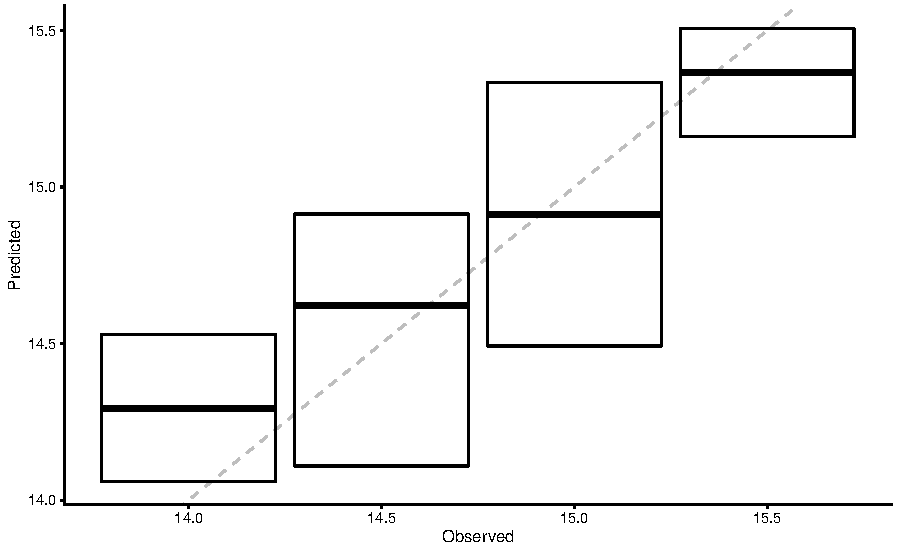
\includegraphics[width=0.9\linewidth]{03-Prediction_files/figure-latex/mas-yoyo-bias-cv-prediction-observation-1} 

}

\caption{\textbf{Testing prediction residuals across cross-validation folds summarized with cross-bars for every observation value.} Cross-bars represent ranges of testing residuals for each observation, while horizontal bar represent mean residual. The length of the bar represents \(Variance\), while distance between horizontal dashed line and horizontal line in the cross-bar (i.e.~mean residual) represents \(Bias\).}\label{fig:mas-yoyo-bias-cv-prediction-observation}
\end{figure}



Cross-validated, \emph{pooled}, and full training data set predictive performance metrics can be found in the Table \ref{tab:mas-yoyo-cv-performance-summary}. Please note that the \emph{pooled} predictive performance metrics are in the column \texttt{testing.pooled}.



\begin{table}

\caption{\label{tab:mas-yoyo-cv-performance-summary}\textbf{Predictive performance summary}}
\centering
\resizebox{\linewidth}{!}{
\begin{tabular}[t]{lrrrrrrr}
\toprule
metric & training & training.pooled & testing.pooled & mean & SD & min & max\\
\midrule
MBE & 0.00 & 0.00 & 0.00 & 0.00 & 0.10 & -0.17 & 0.21\\
MAE & 0.17 & 0.17 & 0.19 & 0.19 & 0.05 & 0.13 & 0.27\\
RMSE & 0.21 & 0.21 & 0.23 & 0.23 & 0.05 & 0.14 & 0.29\\
PPER & 0.97 & 0.98 & 0.97 & 0.94 & 0.04 & 0.87 & 0.99\\
SESOI to RMSE & 4.73 & 4.83 & 4.33 & 4.65 & 1.12 & 3.42 & 7.15\\
\addlinespace
R-squared & 0.74 & 0.75 & 0.68 & 0.68 & 0.18 & 0.27 & 0.87\\
MinErr & -0.44 & -0.49 & -0.51 & -0.33 & 0.13 & -0.51 & -0.06\\
MaxErr & 0.39 & 0.42 & 0.53 & 0.35 & 0.10 & 0.15 & 0.53\\
MaxAbsErr & 0.44 & 0.49 & 0.53 & 0.41 & 0.09 & 0.22 & 0.53\\
\bottomrule
\end{tabular}}
\end{table}

Summary from the Table \ref{tab:mas-yoyo-cv-performance-summary} as well as the individual cross-validated sample predictive performance from the Table \ref{tab:mas-yoyo-cv-performance} are visually represented in the Figure \ref{fig:mas-yoyo-cv-graphical}).

\begin{figure}[!htb]

{\centering 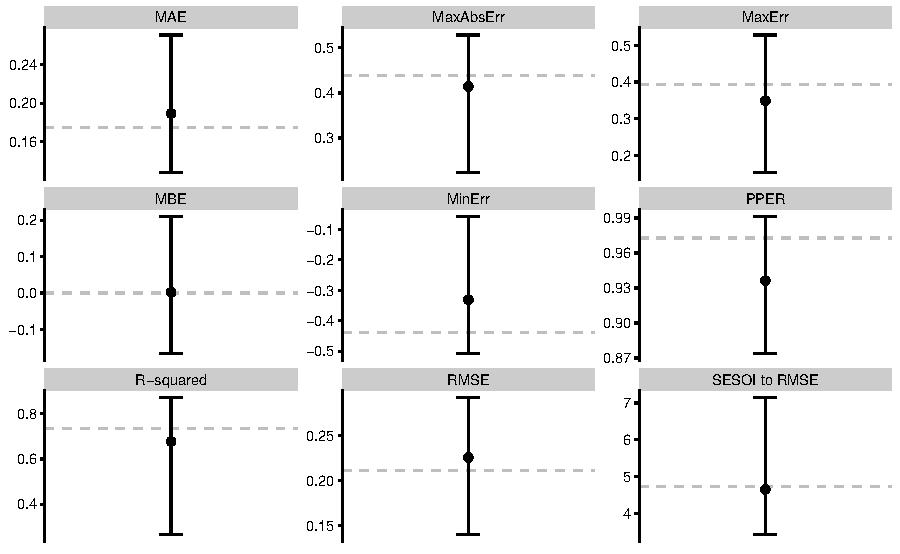
\includegraphics[width=0.9\linewidth]{03-Prediction_files/figure-latex/mas-yoyo-cv-graphical-1} 

}

\caption{\textbf{Cross-validated model performance. }Dot and line bar indicate \texttt{mean}, \texttt{min} and \texttt{max} of the cross-validated performance. Dotted line indicate model performance on the training data set.}\label{fig:mas-yoyo-cv-graphical}
\end{figure}



As can be seen from the Figure \ref{fig:mas-yoyo-cv-graphical}, cross-validated prediction performance metrics do not differ much\footnote{As you will learn in \protect\hyperlink{statistical-inference}{Statistical inference} section, we can perform statistical tests (in this case \emph{t-test}) to check whether the average of the cross-validated performance metric differ from metric estimated on the full training sample.} from the metrics estimated using the full training sample (calculated in \protect\hyperlink{describing-relationship-between-two-variables}{Describing relationship between two variables} section and in the Table \ref{tab:mas-yoyo-training-performance}, and indicated by the dotted horizontal line in the Figure \ref{fig:mas-yoyo-cv-graphical}). For some more complex models, these differences can be much larger and are clear indication of the model over-fitting.

Overall, predicting MAS from the YoYoIR1 score, \emph{given} the data collected, SESOI of ±0.5km/h, and linear regression as a model, is practically excellent. Please note that prediction can be practically useful (given SESOI) (\texttt{PPER}; CV from 0.87 to 0.99) even when \texttt{R-squared} is relatively low (CV from 0.27 to 0.87). And the \emph{vice versa} in some cases. That's the reason why we need to utilize magnitude-based estimators as a complement of contemporary estimators such as \texttt{R-squared}, \texttt{RSE}, and \texttt{RMSE}.

\hypertarget{predicting-yoyoir1-from-mas}{%
\subsection{Predicting YoYoIR1 from MAS}\label{predicting-yoyoir1-from-mas}}

As shown in \protect\hyperlink{describing-relationship-between-two-variables}{Describing relationship between two variables}, predicting YoYoIR1 from MAS scores was not practically useful (or precise enough). But for the sake of completeness, let's perform cross-validated prediction (using 3 folds and 5 repeats). YoYoIR1 SESOI is taken to be ±40m.

Figure \ref{fig:yoyo-mas-ba} depicts modified Bland-Altman plot for predictions using the full training data set. Visual inspection demonstrates that many points are outside of SESOI band, indicating poor practically significant (or useful) predictions.

\begin{figure}[!htb]

{\centering 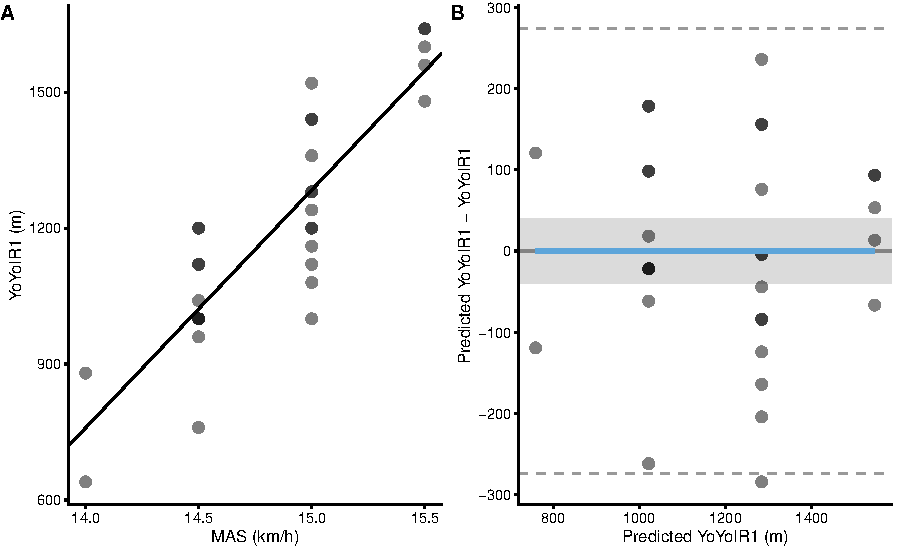
\includegraphics[width=0.9\linewidth]{03-Prediction_files/figure-latex/yoyo-mas-ba-1} 

}

\caption{\textbf{Scatter plot for simple linear regression between YoYoIR1 and MAS using the full training data sample. A. } Scatter plot between YoYoIR1 and MAS scores. Black line indicates model prediction. \textbf{B.} Scatter plot between \(y_{predicted}\) (fitted or predicted YoYoIR1) against model residual \(y_{residual} = y_{predicted} - y_{observed}\), or Predicted YoYoIR1 - YoYoIR1. Dotted lines indicate \emph{Levels of Agreement} (LOA; i.e.~upper and lower threshold that contain 95\% of residuals distribution) and grey band indicates SESOI. Blue line indicate linear regression fit of the residuals and is used to indicate issues with the model (residuals)}\label{fig:yoyo-mas-ba}
\end{figure}



Predictive performance metrics can be found in the Table \ref{tab:mas-yoyo-cv-performance-summary}. As already expected, predicting YoYoIR1 from the MAS score, \textbf{given} the data collected, SESOI and linear regression model is not precise enough to be practically useful. Please note that the \texttt{R-squared} is very close to \texttt{R-squared} from the Table \ref{tab:mas-yoyo-cv-performance-summary}, but the \texttt{PPER} is much worse. Another reason to complement contemporary estimators with magnitude-based ones.



\begin{table}

\caption{\label{tab:yoyo-mas-cv-performance-summary}\textbf{Predictive performance summary}}
\centering
\resizebox{\linewidth}{!}{
\begin{tabular}[t]{lrrrrrrr}
\toprule
metric & training & training.pooled & testing.pooled & mean & SD & min & max\\
\midrule
MBE & 0.00 & 0.00 & 3.13 & 1.95 & 50.33 & -96.20 & 82.14\\
MAE & 104.69 & 103.04 & 112.98 & 112.59 & 24.99 & 66.61 & 154.76\\
RMSE & 129.30 & 127.55 & 138.73 & 135.92 & 26.46 & 82.62 & 175.52\\
PPER & 0.24 & 0.25 & 0.23 & 0.22 & 0.05 & 0.17 & 0.34\\
SESOI to RMSE & 0.62 & 0.63 & 0.58 & 0.61 & 0.14 & 0.46 & 0.97\\
\addlinespace
R-squared & 0.74 & 0.74 & 0.70 & 0.70 & 0.14 & 0.48 & 0.88\\
MinErr & -235.93 & -261.63 & -253.04 & -193.59 & 43.68 & -253.04 & -76.70\\
MaxErr & 284.07 & 309.00 & 323.53 & 225.37 & 89.69 & 51.02 & 323.53\\
MaxAbsErr & 284.07 & 309.00 & 323.53 & 260.89 & 44.88 & 158.47 & 323.53\\
\bottomrule
\end{tabular}}
\end{table}

In the second part of this book, we will get back to this example and estimate predictive performance using different models besides linear regression (like baseline prediction and \emph{regression trees})

\hypertarget{causal-inference}{%
\chapter{Causal inference}\label{causal-inference}}

Does playing basketball makes one taller? This is a an example of a causal question. Wrestling with the concept of causality, as a philosophical construct is outside the scope of this book (and the author too), but I will define it using the \emph{counterfactual theory} or \emph{potential outcomes} perspective (Hernán, Hsu, and Healy \protect\hyperlink{ref-hernanSecondChanceGet2019}{2019}; Kleinberg \protect\hyperlink{ref-kleinbergWhyGuideFinding2015}{2015}; Pearl and Mackenzie \protect\hyperlink{ref-pearlBookWhyNew2018}{2018}; Angrist and Pischke \protect\hyperlink{ref-angristMasteringMetricsPath2015}{2015}; Gelman \protect\hyperlink{ref-gelmanCausalityStatisticalLearning2011}{2011}) that define causes in terms of how things would have been different had the cause not occurred, as well as from \emph{causality-as-intervention} perspective (Gelman \protect\hyperlink{ref-gelmanCausalityStatisticalLearning2011}{2011}), which necessitates clearly defined interventions (Hernán \protect\hyperlink{ref-hernanCWordScientificEuphemisms2018}{2018}, \protect\hyperlink{ref-hernanDoesWaterKill2016}{2016}; Hernán and Taubman \protect\hyperlink{ref-hernanDoesObesityShorten2008}{2008}). In other words, would someone be shorter if basketball was never trained?

There are two broad classes of inferential questions that focus on \emph{what if} and \emph{why}: \emph{forward causal inference} (``What might happen if we do \emph{X}?'') and \emph{reverse causal inference} (``What causes \emph{Y}? Why?'') (Gelman \protect\hyperlink{ref-gelmanCausalityStatisticalLearning2011}{2011}). Forward causation is more clearly defined problem, where the goal is to quantify the causal effect of treatment. Questions of forward causation are most directly studied using \emph{randomization} (Gelman \protect\hyperlink{ref-gelmanCausalityStatisticalLearning2011}{2011}) and are answered from the above mentioned causality-as-intervention and counterfactual perspectives. Reverse causation is more complex and it is more related to \emph{explaining} the causal chains using the \emph{system-variable} approach. Article by Gelman (\protect\hyperlink{ref-gelmanCausalityStatisticalLearning2011}{2011}) provides great overview of the most common causal perspectives, out of which I will mostly focus on forward causation.

\hypertarget{necessary-versus-sufficient-causality}{%
\section{Necessary versus sufficient causality}\label{necessary-versus-sufficient-causality}}

Furthermore, we also need to distinguish between four kinds of causation (Pearl and Mackenzie \protect\hyperlink{ref-pearlBookWhyNew2018}{2018}; Kleinberg \protect\hyperlink{ref-kleinbergWhyGuideFinding2015}{2015}): \emph{necessary causation}, \emph{sufficient causation} and neither or both. For example, if someone says that A causes B, then:

\begin{itemize}
\tightlist
\item
  If A is \emph{necessary} for B, it means that if A never happened (counterfactual reasoning), then B will never happen. Or, in other words, B can never happen without A. But sufficient causality also means that A can happen without B happening.
\item
  If A is \emph{sufficient} for B, it means that if you have A, you will \emph{always} have B. In other words, B always follows A. However, sometimes B can happen without A
\item
  If A is \emph{neither sufficient nor necessary} for B, then sometimes when A happens B will happen. B can also happen without A.
\item
  If A is both necessary and sufficient for B, then B will always happen after A, and B will never happen without A.
\end{itemize}

Table \ref{tab:four-causes-table} contains summary of the above necessary and sufficient causality. In all four types of causation, the concept of counterfactual reasoning is invoked.



\begin{table}

\caption{\label{tab:four-causes-table}\textbf{Four kinds of causation}}
\centering
\resizebox{\linewidth}{!}{
\begin{tabular}[t]{lllll}
\toprule
Cause & Necessary & Sufficient & Neither & Both\\
\midrule
A happens & B might happen & B always happen & B might happen & B always happen\\
A doesn't happen & B never happens & B might happen & B might happen & B never happens\\
\bottomrule
\end{tabular}}
\end{table}

Although the causal inference is a broad area of research, philosophical discussion and conflicts, there are a few key concepts that need to be introduced to get the big picture and understand the basics behind the aims of causal inference. Let's start with an example involving the aforementioned question whether playing basketball makes one taller.

\hypertarget{observational-data}{%
\section{Observational data}\label{observational-data}}

In order to answer this question, we have collected height data (expressed in cm) for the total of N=30 athletes, of which N=15 play basketball, and N=15 don't play basketball (Table \ref{tab:basketball-data}). Playing basketball can be considered \emph{intervention} or \emph{treatment}, in which causal effect we are interested in. Basketball players are considered \emph{intervention group} or \emph{treatment group} and those without the treatment are considered \emph{comparison group} or \emph{control group}



\begin{table}

\caption{\label{tab:basketball-data}\textbf{Height in the treatment and control groups}}
\centering
\begin{tabular}[t]{llr}
\toprule
Athlete & Treatment & Height (cm)\\
\midrule
Athlete 27 & Basketball & 214\\
Athlete 01 & Basketball & 214\\
Athlete 25 & Basketball & 211\\
Athlete 19 & Basketball & 210\\
Athlete 03 & Basketball & 207\\
\addlinespace
Athlete 21 & Basketball & 200\\
Athlete 23 & Basketball & 199\\
Athlete 15 & Basketball & 198\\
Athlete 17 & Basketball & 193\\
Athlete 07 & Basketball & 192\\
\addlinespace
Athlete 29 & Basketball & 192\\
Athlete 13 & Basketball & 191\\
Athlete 05 & Basketball & 191\\
Athlete 11 & Basketball & 184\\
Athlete 09 & Basketball & 180\\
\addlinespace
Athlete 02 & Control & 189\\
Athlete 28 & Control & 183\\
Athlete 06 & Control & 181\\
Athlete 14 & Control & 180\\
Athlete 04 & Control & 179\\
\addlinespace
Athlete 12 & Control & 176\\
Athlete 18 & Control & 176\\
Athlete 08 & Control & 173\\
Athlete 26 & Control & 173\\
Athlete 24 & Control & 170\\
\addlinespace
Athlete 30 & Control & 168\\
Athlete 20 & Control & 168\\
Athlete 16 & Control & 165\\
Athlete 10 & Control & 165\\
Athlete 22 & Control & 163\\
\bottomrule
\end{tabular}
\end{table}

Using descriptive estimators introduced in the \protect\hyperlink{description}{Description} section, one can quickly calculate the group \texttt{mean} and \texttt{SD} as well as their difference (Table \ref{tab:descriptive-group-analysis}). But does mean difference between basketball and control represent \emph{average causal effect} (ACE)\footnote{Another term used is \emph{average treatment effect} (ATE)}? No, unfortunately not!



\begin{table}

\caption{\label{tab:descriptive-group-analysis}\textbf{Descriptive analysis of the groups}}
\centering
\begin{tabular}[t]{lrr}
\toprule
 & Mean (cm) & SD (cm)\\
\midrule
Basketball & 198.59 & 10.86\\
Control & 174.04 & 7.54\\
Difference & 24.55 & 13.22\\
\bottomrule
\end{tabular}
\end{table}

\hypertarget{potential-outcomes-or-counterfactuals}{%
\section{Potential outcomes or counterfactuals}\label{potential-outcomes-or-counterfactuals}}

To explain why this is the case, we need to imagine \emph{alternate counterfactual reality}. What is needed are two potential outcomes: \(Height_{0}\), which represents height of the person if one doesn't train basketball, and \(Height_{1}\) which represents height of the person if basketball is being played (Table \ref{tab:basketball-counterfactuals}). As can be guessed, the Basketball group has known \(Height_{1}\), but unknown \(Height_{0}\) and \emph{vice versa} for the Control group.



\begin{table}

\caption{\label{tab:basketball-counterfactuals}\textbf{Counterfactuals of potential outcomes that are unknown}}
\centering
\resizebox{\linewidth}{!}{
\begin{tabular}[t]{llrrrl}
\toprule
Athlete & Treatment & Height\_0 (cm) & Height\_1 (cm) & Height (cm) & Causal Effect (cm)\\
\midrule
Athlete 27 & Basketball & ??? & 214 & 214 & ???\\
Athlete 01 & Basketball & ??? & 214 & 214 & ???\\
Athlete 25 & Basketball & ??? & 211 & 211 & ???\\
Athlete 19 & Basketball & ??? & 210 & 210 & ???\\
Athlete 03 & Basketball & ??? & 207 & 207 & ???\\
\addlinespace
Athlete 21 & Basketball & ??? & 200 & 200 & ???\\
Athlete 23 & Basketball & ??? & 199 & 199 & ???\\
Athlete 15 & Basketball & ??? & 198 & 198 & ???\\
Athlete 17 & Basketball & ??? & 193 & 193 & ???\\
Athlete 07 & Basketball & ??? & 192 & 192 & ???\\
\addlinespace
Athlete 29 & Basketball & ??? & 192 & 192 & ???\\
Athlete 13 & Basketball & ??? & 191 & 191 & ???\\
Athlete 05 & Basketball & ??? & 191 & 191 & ???\\
Athlete 11 & Basketball & ??? & 184 & 184 & ???\\
Athlete 09 & Basketball & ??? & 180 & 180 & ???\\
\addlinespace
Athlete 02 & Control & 189 & ??? & 189 & ???\\
Athlete 28 & Control & 183 & ??? & 183 & ???\\
Athlete 06 & Control & 181 & ??? & 181 & ???\\
Athlete 14 & Control & 180 & ??? & 180 & ???\\
Athlete 04 & Control & 179 & ??? & 179 & ???\\
\addlinespace
Athlete 12 & Control & 176 & ??? & 176 & ???\\
Athlete 18 & Control & 176 & ??? & 176 & ???\\
Athlete 08 & Control & 173 & ??? & 173 & ???\\
Athlete 26 & Control & 173 & ??? & 173 & ???\\
Athlete 24 & Control & 170 & ??? & 170 & ???\\
\addlinespace
Athlete 30 & Control & 168 & ??? & 168 & ???\\
Athlete 20 & Control & 168 & ??? & 168 & ???\\
Athlete 16 & Control & 165 & ??? & 165 & ???\\
Athlete 10 & Control & 165 & ??? & 165 & ???\\
Athlete 22 & Control & 163 & ??? & 163 & ???\\
\bottomrule
\end{tabular}}
\end{table}

Unfortunately, these potential outcomes are unknown, and thus individual causal effects are unknown as well. We just do not know what might have happened to individual outcomes in counterfactual world (i.e.~alternate reality). A good control group serves as a \emph{proxy} to reveal what might have happened \emph{on average} to the treated group in the counterfactual world where they are not treated. Since the basketball data is simulated, the exact DGP is known (the \emph{true} systematic or main causal effect of playing basketball on height is exactly zero), which again demonstrates the use of simulations as a great learning tool, in this case understanding the underlying causal mechanisms (Table \ref{tab:table-counterfactuals-simulated}). Individual causal effect in this case is the difference between two potential outcomes: \(Height_{1}\) and \(Height_{0}\).



\begin{table}

\caption{\label{tab:table-counterfactuals-simulated}\textbf{Simulated causal effects and known counterfactuals}}
\centering
\resizebox{\linewidth}{!}{
\begin{tabular}[t]{llrrrr}
\toprule
Athlete & Treatment & Height\_0 (cm) & Height\_1 (cm) & Height (cm) & Causal Effect (cm)\\
\midrule
Athlete 27 & Basketball & 214 & 214 & 214 & 0.12\\
Athlete 01 & Basketball & 214 & 214 & 214 & 0.00\\
Athlete 25 & Basketball & 212 & 211 & 211 & -1.10\\
Athlete 19 & Basketball & 210 & 210 & 210 & 0.90\\
Athlete 03 & Basketball & 208 & 207 & 207 & -0.07\\
\addlinespace
Athlete 21 & Basketball & 200 & 200 & 200 & 0.20\\
Athlete 23 & Basketball & 198 & 199 & 199 & 0.57\\
Athlete 15 & Basketball & 198 & 198 & 198 & 0.18\\
Athlete 17 & Basketball & 193 & 193 & 193 & 0.44\\
Athlete 07 & Basketball & 193 & 192 & 192 & -0.09\\
\addlinespace
Athlete 29 & Basketball & 193 & 192 & 192 & -0.40\\
Athlete 13 & Basketball & 192 & 191 & 191 & -0.36\\
Athlete 05 & Basketball & 191 & 191 & 191 & -0.15\\
Athlete 11 & Basketball & 183 & 184 & 184 & 0.46\\
Athlete 09 & Basketball & 179 & 180 & 180 & 0.72\\
\addlinespace
Athlete 02 & Control & 189 & 189 & 189 & 0.06\\
Athlete 28 & Control & 183 & 184 & 183 & 0.41\\
Athlete 06 & Control & 181 & 181 & 181 & 0.42\\
Athlete 14 & Control & 180 & 180 & 180 & -0.66\\
Athlete 04 & Control & 179 & 179 & 179 & 0.10\\
\addlinespace
Athlete 12 & Control & 176 & 176 & 176 & -0.39\\
Athlete 18 & Control & 176 & 175 & 176 & -0.31\\
Athlete 08 & Control & 173 & 173 & 173 & -0.55\\
Athlete 26 & Control & 173 & 174 & 173 & 0.77\\
Athlete 24 & Control & 170 & 170 & 170 & 0.02\\
\addlinespace
Athlete 30 & Control & 168 & 168 & 168 & 0.27\\
Athlete 20 & Control & 168 & 168 & 168 & -0.03\\
Athlete 16 & Control & 165 & 165 & 165 & -0.01\\
Athlete 10 & Control & 165 & 164 & 165 & -0.81\\
Athlete 22 & Control & 163 & 163 & 163 & 0.00\\
\bottomrule
\end{tabular}}
\end{table}

From Table \ref{tab:table-counterfactuals-simulated}, we can state that the mean difference between the groups consists of two components: \emph{average causal effect} and the \emph{selection bias} (Angrist and Pischke \protect\hyperlink{ref-angristMasteringMetricsPath2015}{2015}) (Equation \eqref{eq:mean-causal-effect}).

\begin{equation}
  \begin{split}
    mean_{difference} &= Average \; causal\; effect + Selection\; bias \\
    Average \; causal\; effect &= \frac{1}{N_{Basketball}}\Sigma_{i=1}^{n}(Height_{1i} - Height_{0i}) \\
    Selection\; bias &= \frac{1}{N_{Basketball}}\Sigma_{i=1}^{n}Height_{0i} - \frac{1}{N_{Control}}\Sigma_{i=1}^{n}Height_{0i}
  \end{split}
  \label{eq:mean-causal-effect}
\end{equation}

The mean group difference we have observed (24.55cm) is due to average causal effect (0.1cm) and selection bias (24.46cm). In other words, observed mean group difference can be explained solely by selection bias. Since we know the DGP behind the basketball data, we know that there is no systematic causal effect of playing basketball on height.

On top of the selection bias involved in the example above, other \emph{confounders} might be involved, such as age, sex, race, experience and others, some of which can be measured and some might be unknown. These are also referred to as the \emph{third variable} which confounds the causal relationship between treatment and the outcome. In this example, all subjects from the Basketball group might be older males, whereas all the subjects from the Control group might be be younger females, and this can explain the group differences, rather than causal effect of playing basketball.

\hypertarget{ceteris-paribus-and-the-biases}{%
\section{\texorpdfstring{\emph{Ceteris paribus} and the biases}{Ceteris paribus and the biases}}\label{ceteris-paribus-and-the-biases}}

It is important to understand that, in order to have causal interpretation, comparisons need to be made under \emph{ceteris paribus} conditions (Angrist and Pischke \protect\hyperlink{ref-angristMasteringMetricsPath2015}{2015}), which is Latin for \emph{other things equal}. In the basketball example above, we cannot make causal claim that playing basketball makes one taller, since comparison between the groups is not done in the \emph{ceteris paribus} conditions due to the selection bias involved. We also know this since we know the DGP behind the observed data.

Causal inference thus aims to achieve \emph{ceteris paribus} conditions needed to make causal interpretations by careful considerations of the known and unknown biases involved (Angrist and Pischke \protect\hyperlink{ref-angristMasteringMetricsPath2015}{2015}; Hernán \protect\hyperlink{ref-hernanCausalDiagramsDraw2017}{2017}, \protect\hyperlink{ref-hernanDoesWaterKill2016}{2016}; Hernán and Robins, \protect\hyperlink{ref-hernanCausalInference2019}{n.d.}; Hernán, Hsu, and Healy \protect\hyperlink{ref-hernanSecondChanceGet2019}{2019}; Lederer et al. \protect\hyperlink{ref-ledererControlConfoundingReporting2019}{2019}; Rohrer \protect\hyperlink{ref-rohrerThinkingClearlyCorrelations2018}{2018}; Shrier and Platt \protect\hyperlink{ref-shrierReducingBiasDirected2008}{2008}).

According to Hernan \emph{et al.} (Hernán \protect\hyperlink{ref-hernanCausalDiagramsDraw2017}{2017}; Hernán and Robins, \protect\hyperlink{ref-hernanCausalInference2019}{n.d.}), there are three types of biases involved in causal inference: \emph{confounding}, \emph{selection bias} and \emph{measurement bias}.

Confounding is the bias that arises when treatment and outcome share causes. This is because treatment was not randomly assigned (Hernán \protect\hyperlink{ref-hernanCausalDiagramsDraw2017}{2017}; Hernán and Robins, \protect\hyperlink{ref-hernanCausalInference2019}{n.d.}). For example, athletes that are naturally taller might be choosing to play basketball due to success and enjoyment over their shorter peers. On the other hand, it might be some hidden confounder that motivates \emph{to-be-tall} athletes to choose basketball. Known and measured confounders from the observational studies can be taken into account to create \emph{ceteris paribus} conditions when estimating causal effects (Angrist and Pischke \protect\hyperlink{ref-angristMasteringMetricsPath2015}{2015}; Hernán \protect\hyperlink{ref-hernanCausalDiagramsDraw2017}{2017}; Hernán and Robins, \protect\hyperlink{ref-hernanCausalInference2019}{n.d.}; Lederer et al. \protect\hyperlink{ref-ledererControlConfoundingReporting2019}{2019}; Rohrer \protect\hyperlink{ref-rohrerThinkingClearlyCorrelations2018}{2018}; Shrier and Platt \protect\hyperlink{ref-shrierReducingBiasDirected2008}{2008}).

\hypertarget{randomization}{%
\subsection{Randomization}\label{randomization}}

The first line of defence against confounding and selection bias is to randomly assign athletes to treatment, otherwise known as \emph{randomized trial} or \emph{randomized experiment}. Random assignment makes comparison between groups \emph{ceteris paribus} providing the sample is large enough to ensure that differences in the individual characteristics such as age, sex, experience and other potential confounders are \emph{washed out} (Angrist and Pischke \protect\hyperlink{ref-angristMasteringMetricsPath2015}{2015}). In other words, random assignment works not by eliminating individual differences but rather by ensuring that the mix of the individuals being compared is the same, including the ways we cannot easily measure or observe (Angrist and Pischke \protect\hyperlink{ref-angristMasteringMetricsPath2015}{2015}).

In case the individuals from the basketball example were randomly assigned, given the known causal DGP, then the mean difference between the groups would be more indicative of the causal effect of playing basketball on height (Table \ref{tab:randomized-basketball-data}).



\begin{table}

\caption{\label{tab:randomized-basketball-data}\textbf{Randomized participants}}
\centering
\begin{tabular}[t]{llr}
\toprule
Athlete & Treatment & Height (cm)\\
\midrule
Athlete 01 & Basketball & 214\\
Athlete 25 & Basketball & 211\\
Athlete 19 & Basketball & 210\\
Athlete 03 & Basketball & 207\\
Athlete 23 & Basketball & 199\\
\addlinespace
Athlete 15 & Basketball & 198\\
Athlete 13 & Basketball & 191\\
Athlete 02 & Basketball & 189\\
Athlete 28 & Basketball & 184\\
Athlete 14 & Basketball & 180\\
\addlinespace
Athlete 04 & Basketball & 179\\
Athlete 12 & Basketball & 176\\
Athlete 26 & Basketball & 174\\
Athlete 24 & Basketball & 170\\
Athlete 16 & Basketball & 165\\
\addlinespace
Athlete 27 & Control & 214\\
Athlete 21 & Control & 200\\
Athlete 29 & Control & 193\\
Athlete 07 & Control & 193\\
Athlete 17 & Control & 193\\
\addlinespace
Athlete 05 & Control & 191\\
Athlete 11 & Control & 183\\
Athlete 06 & Control & 181\\
Athlete 09 & Control & 179\\
Athlete 18 & Control & 176\\
\addlinespace
Athlete 08 & Control & 173\\
Athlete 30 & Control & 168\\
Athlete 20 & Control & 168\\
Athlete 10 & Control & 165\\
Athlete 22 & Control & 163\\
\bottomrule
\end{tabular}
\end{table}

If we calculate the mean differences in this randomly assigned basketball treatment (Table \ref{tab:basketball-randomized-summary}), we can quickly notice that random assignment washed out selection bias involved with the observational study, and that the mean difference is closer to the known systematic (or average or \emph{expected}) causal effect. The difference between estimated systematic causal effect using mean group difference from the randomized trial and the true causal effect is due to the \emph{sampling error} which will be explained in the \protect\hyperlink{statistical-inference}{Statistical inference} section.



\begin{table}

\caption{\label{tab:basketball-randomized-summary}\textbf{Descriptive summary of randomized participants}}
\centering
\begin{tabular}[t]{lrr}
\toprule
 & Mean (cm) & SD (cm)\\
\midrule
Basketball & 189.91 & 16.15\\
Control & 182.65 & 14.44\\
Difference & 7.25 & 21.66\\
\bottomrule
\end{tabular}
\end{table}

Apart from creating \emph{ceteris paribus} conditions, randomization generates a good control group that serves as a \emph{proxy} to reveal what might have happened to the treated group in the counterfactual world where they are not treated, since \(Height_0\) is not known for the basketball group. Creating those conditions with randomized trial demands careful considerations and \emph{balance checking} since biases can \emph{crawl} inside the causal interpretation. The logic of randomized trial is simple, yet the logistics can be quite complex. For example, a sample of sufficient size might not be practically feasible, and imbalances in the known confounders can be still found in the groups, thus demanding further control and adjustment in the analysis (e.g.~using ANCOVA instead of ANOVA, adjusting for confounders in the linear regression by introducing them as interactions) in order to create \emph{ceteris paribus} conditions needed to evaluate causal claims. Belief effect can sneak in, for example, if the treatment group \emph{knows} they are being treated, or if researchers motivate treatment groups harder, since they expect and hope for better outcomes. For this reason, \emph{blinding} both the subjects and researches can be considered, as well as providing \emph{placebo} treatment to the Control group. In sport science research blinding and providing placebo can be problematic. For example, if our intervention is a novel training method or a technology, both researchers and subjects will expect better outcomes which can bias causal interpretations.

\hypertarget{subject-matter-knowledge}{%
\section{Subject matter knowledge}\label{subject-matter-knowledge}}

One of the main problems with randomized trials is that it cannot be done in most real life settings, either due to the ethical or practical reasons. For example, if studying effects of smoking on baby mortality and birth defects, which parent would accept being in the treatment group. Or if studying effects of resistance training on injury risk in football players, which professional organization would allow random assignment to the treatment that is lesser than the known best practices and can predispose athletes to the injuries or sub-par preparation?

For this reason, reliance on observation studies is the best we can do. However, in order to create \emph{ceteris paribus} conditions necessary to minimize bias in the causal interpretations, expert subject-matter knowledge is needed, not only to describe the causal structure of the system under study, but also to specify the causal questions and identify relevant data sources (Hernán, Hsu, and Healy \protect\hyperlink{ref-hernanSecondChanceGet2019}{2019}). Imagine asking the following causal question: ``Does training load lead to overuse injuries in professional sports''. It takes expert subject matter knowledge to specify the treatment construct (i.e.~``training load''), to figure out how should be measured, as well as to quantify the measurement error which can induce \emph{measurement bias}, to state over which time period the treatment is done, as well as to specify the outcome construct (i.e.~``overuse-injuries''), and to define the variables and constructs that confound and define the causal network underlying such a question. This subject matter is fallible of course, and the constructs, variables and the causal network can be represented with pluralistic models that represents ``Small World'' maps of the complex ``Large World'', in which we are hoping to deploy the findings (please refer to the \protect\hyperlink{introduction}{Introduction} for more information about this concept). Drawing assumptions that underly causal structure using \emph{direct acyclical graphs} (DAGs) (Hernán \protect\hyperlink{ref-hernanCausalDiagramsDraw2017}{2017}; Hernán and Robins, \protect\hyperlink{ref-hernanCausalInference2019}{n.d.}; Pearl and Mackenzie \protect\hyperlink{ref-pearlBookWhyNew2018}{2018}; Rohrer \protect\hyperlink{ref-rohrerThinkingClearlyCorrelations2018}{2018}; Saddiki and Balzer \protect\hyperlink{ref-saddikiPrimerCausalityData2018}{2018}; Shrier and Platt \protect\hyperlink{ref-shrierReducingBiasDirected2008}{2008}; Textor et al. \protect\hyperlink{ref-textorRobustCausalInference2017}{2017}) represents a step forward in acknowledging the issues above, by providing transparency of the assumptions involved and bridging the subjective - objective dichotomy.

\hypertarget{example-of-randomized-control-trial}{%
\section{Example of randomized control trial}\label{example-of-randomized-control-trial}}

Let's consider the following example. We are interested in estimating causal effect of the plyometric training on the vertical jump height. To estimate causal effect, \emph{randomized control trial} (RCT) is utilized. RCT utilizes two groups: Treatment (N=15) and Control (N=15), measured two times: Pre-test and Post-test. Treatment group received plyometric training over the course of three months, while Control group continued with \emph{normal} training. The results of RCT study can be found in the Table \ref{tab:rct-vj-data}. To estimate practical significance of the treatment effect, SESOI of ±2.5cm is selected to indicate minimal change of the practical value. It is important to have ``well defined interventions'' (Hernán \protect\hyperlink{ref-hernanCWordScientificEuphemisms2018}{2018}, \protect\hyperlink{ref-hernanDoesWaterKill2016}{2016}; Hernán and Taubman \protect\hyperlink{ref-hernanDoesObesityShorten2008}{2008}), thus the question that should be answered is as follows: ``Does plyometric training added to normal training improves vertical jump height over period of three months?''



\begin{table}

\caption{\label{tab:rct-vj-data}\textbf{Randomized control trial data}}
\centering
\resizebox{\linewidth}{!}{
\begin{tabular}[t]{llrrr}
\toprule
Athlete & Group & Pre-test (cm) & Post-test (cm) & Change (cm)\\
\midrule
Athlete 01 & Treatment & 37.98 & 52.86 & 14.93\\
Athlete 27 & Treatment & 44.79 & 58.50 & 13.43\\
Athlete 19 & Treatment & 46.77 & 59.76 & 12.99\\
Athlete 25 & Treatment & 38.90 & 49.58 & 10.81\\
Athlete 03 & Treatment & 41.29 & 51.41 & 10.34\\
\addlinespace
Athlete 23 & Treatment & 48.41 & 57.57 & 8.58\\
Athlete 17 & Treatment & 44.81 & 51.41 & 7.85\\
Athlete 21 & Treatment & 37.14 & 44.95 & 7.37\\
Athlete 15 & Treatment & 46.69 & 52.73 & 6.14\\
Athlete 29 & Treatment & 42.77 & 47.38 & 5.02\\
\addlinespace
Athlete 13 & Treatment & 49.66 & 54.11 & 4.46\\
Athlete 05 & Treatment & 37.92 & 41.63 & 3.78\\
Athlete 07 & Treatment & 41.03 & 45.41 & 3.42\\
Athlete 11 & Treatment & 45.27 & 46.72 & 1.82\\
Athlete 12 & Control & 42.56 & 44.29 & 1.01\\
\addlinespace
Athlete 28 & Control & 47.06 & 47.98 & 0.55\\
Athlete 04 & Control & 44.53 & 45.13 & 0.12\\
Athlete 02 & Control & 49.63 & 48.86 & -0.01\\
Athlete 08 & Control & 41.11 & 42.13 & -0.45\\
Athlete 26 & Control & 42.31 & 41.61 & -0.51\\
\addlinespace
Athlete 06 & Control & 45.96 & 45.70 & -0.52\\
Athlete 14 & Control & 44.51 & 42.89 & -0.63\\
Athlete 18 & Control & 42.57 & 42.15 & -0.74\\
Athlete 16 & Control & 37.63 & 37.83 & -0.75\\
Athlete 22 & Control & 36.52 & 34.83 & -0.97\\
\addlinespace
Athlete 24 & Control & 40.15 & 39.88 & -1.03\\
Athlete 30 & Control & 39.34 & 38.34 & -1.21\\
Athlete 09 & Treatment & 47.61 & 45.62 & -1.57\\
Athlete 20 & Control & 38.94 & 36.97 & -1.72\\
Athlete 10 & Control & 36.77 & 34.15 & -2.26\\
\bottomrule
\end{tabular}}
\end{table}

Descriptive summary statistics for Treatment and Control groups are enlisted in the Table \ref{tab:rct-summary}, and visually depicted in the Figure \ref{fig:rct-groups}.



\begin{table}

\caption{\label{tab:rct-summary}\textbf{RCT summary using mean ± SD}}
\centering
\begin{tabular}[t]{llll}
\toprule
Group & Pre-test (cm) & Post-test (cm) & Change (cm)\\
\midrule
Treatment & 43.4 ± 4.15 & 50.64 ± 5.4 & 7.29 ± 4.65\\
Control & 41.97 ± 3.87 & 41.52 ± 4.49 & -0.61 ± 0.83\\
\bottomrule
\end{tabular}
\end{table}

\begin{figure}[!htb]

{\centering 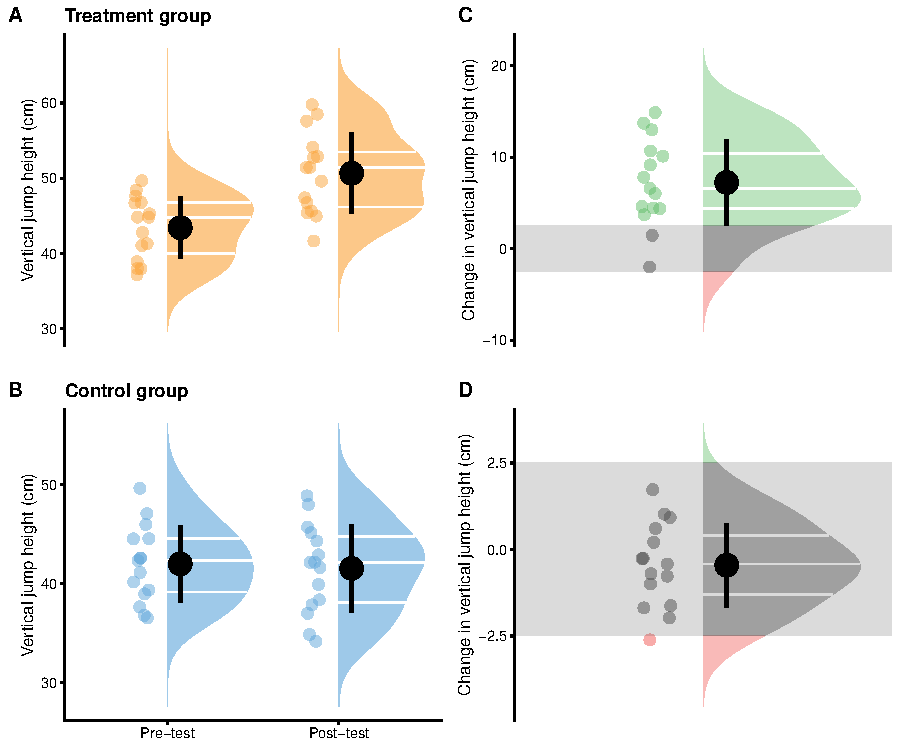
\includegraphics[width=0.9\linewidth]{04-Causal-inference_files/figure-latex/rct-groups-1} 

}

\caption{\textbf{Visual analysis of RCT using Treatment and Control groups. A and B. }Raincloud plot of the Pre-test and Post-test scores for Treatment and Control groups. Blue color indicates Control group and orange color indicates Treatment group. \textbf{C and D.} Raincloud plot of the change scores for the Treatment and Control groups. SESOI is indicated with a grey band}\label{fig:rct-groups}
\end{figure}



Further analysis might involve separate dependent groups analysis for both Treatment and Control (Table \ref{tab:rct-change}), or in other words, the analysis of the change scores. To estimate \texttt{Cohen\textquotesingle{}s\ d}, \texttt{pooled\ SD} of the Pre-test scores in both Treatment and Control is utilized. (see Equation \eqref{eq:cohen-diff-equation}).



\begin{table}

\caption{\label{tab:rct-change}\textbf{Descriptive analysis of the change scores for Treatment and Control groups independently}}
\centering
\begin{tabular}[t]{lrr}
\toprule
Estimator & Control & Treatment\\
\midrule
Mean change (cm) & -0.61 & 7.29\\
SDchange (cm) & 0.83 & 4.65\\
SDpre-test pooled (cm) & 4.01 & 4.01\\
Cohen's d & -0.15 & 1.82\\
SESOI lower (cm) & -2.50 & -2.50\\
\addlinespace
SESOI upper (cm) & 2.50 & 2.50\\
Change to SESOI & -0.12 & 1.46\\
SDchange to SESOI & 0.17 & 0.93\\
pLower & 0.06 & 0.03\\
pEquivalent & 0.93 & 0.14\\
\addlinespace
pHigher & 0.01 & 0.83\\
\bottomrule
\end{tabular}
\end{table}

Figure \ref{fig:rct-paired-change} depicts same information as Figure \ref{fig:rct-groups} but organized differently and conveying different comparison.

\begin{figure}[!htb]

{\centering 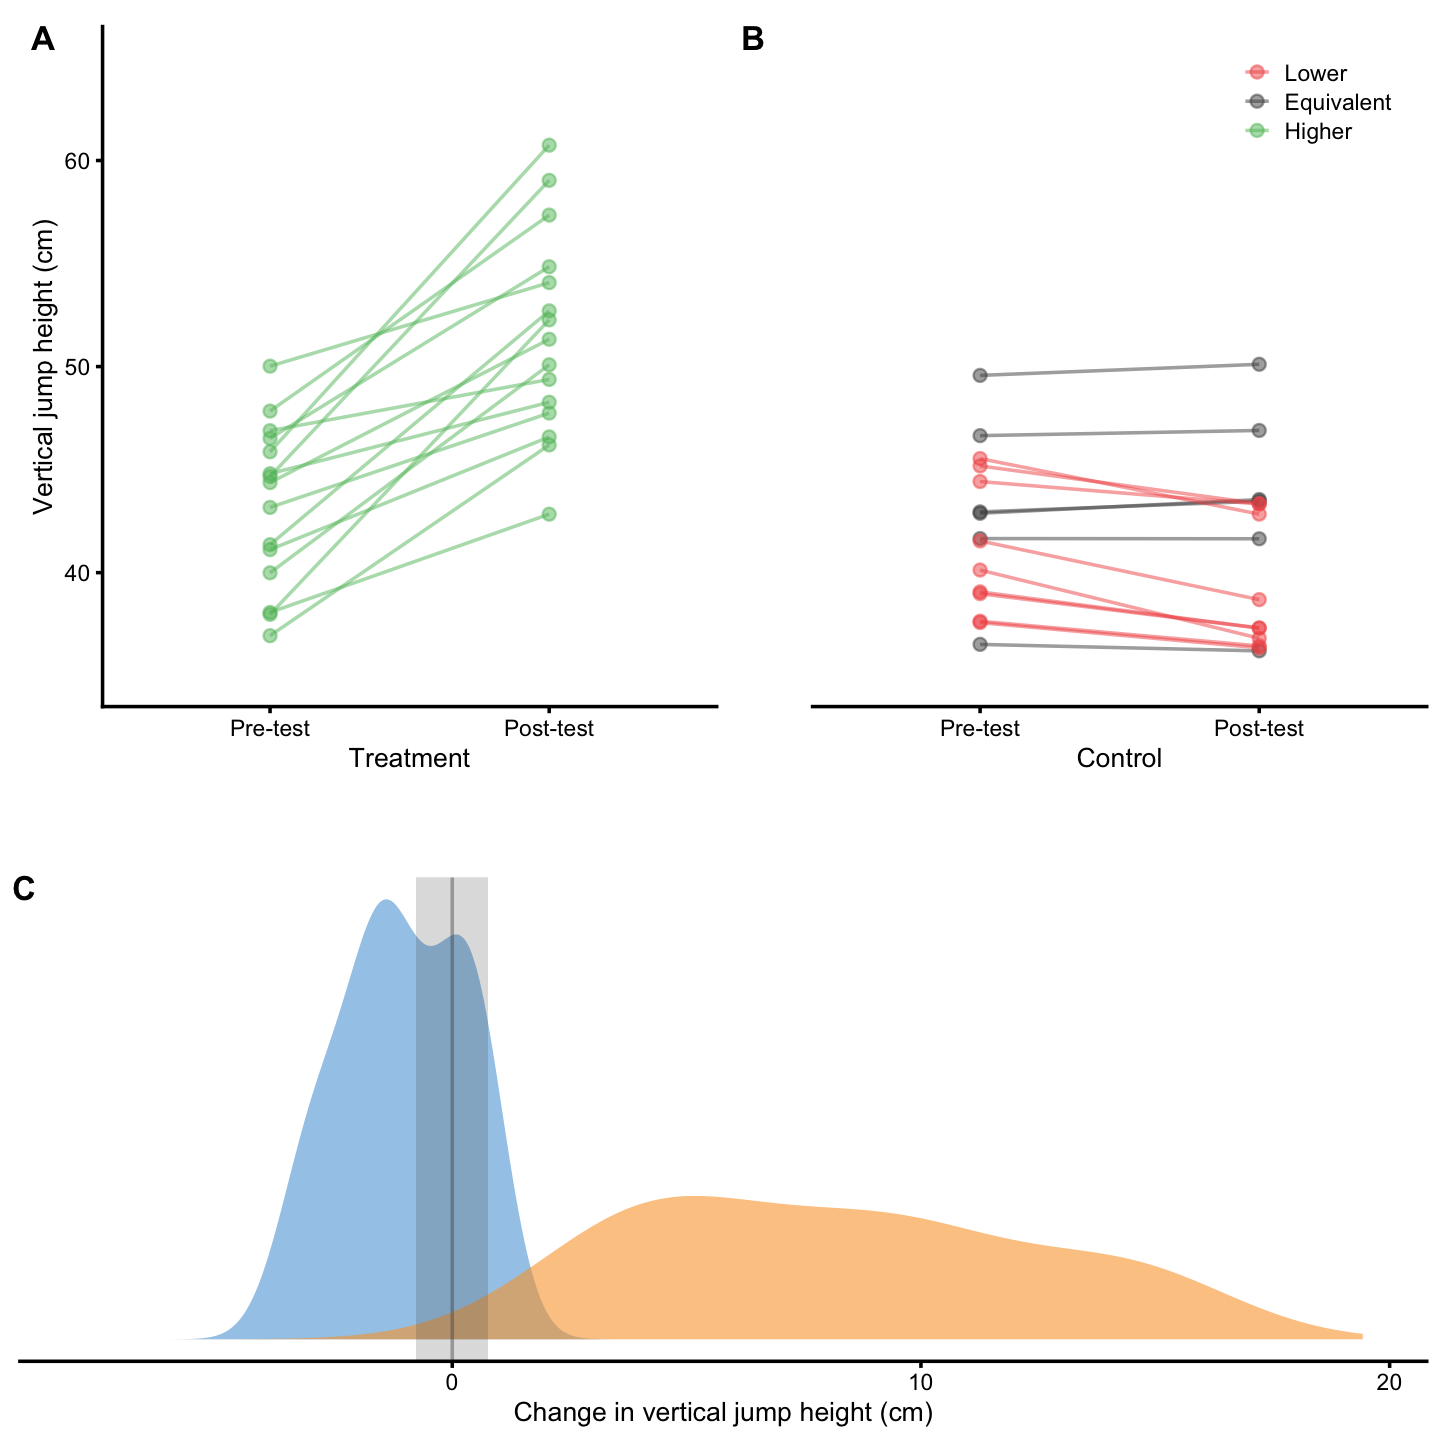
\includegraphics[width=0.9\linewidth]{04-Causal-inference_files/figure-latex/rct-paired-change-1} 

}

\caption{\textbf{Visual analysis of RCT using Treatment and Control groups. A and B. }Scatter plot of Pre-test and Post-test scores for Treatment and Control groups. Green line indicates change higher than SESOI upper, grey line indicates change within SESOI band, and red line indicates negative change lower than SESOI lower. \textbf{C. } Distribution of the change scores for Treatment (orange) and Control (blue) groups. Grey rectangle indicates SESOI band.}\label{fig:rct-paired-change}
\end{figure}



But we are not that interested in independent analysis of Treatment and Control groups, but rather on their differences and understanding of the causal effect of the treatment (i.e.~understanding and estimating parameters of the underlying DGP). As stated, treatment effect consists of two components: systematic component or main effect (i.e.~expected or average causal effect), and stochastic component or random effect (i.e.~that varies between individuals) (see Figure \ref{fig:te-and-nte-diagram}). As already explained, Control group serves as a proxy to what might have happened to the Treatment group in the counterfactual world, and thus allows for casual interpretation of the treatment effect. There are two effects at play with this RCT design: \emph{treatment effect} and \emph{non-treatment effect}. The latter captures all effects not directly controlled by a treatment, but assumes it affects both groups equally (Figure \ref{fig:te-and-nte-diagram}). For example, if we are treating kids for longer period of time, non-treatment effect might be related to the growth and associated effects. Another non-treatment effect is \emph{measurement error} (discussed in more details in \protect\hyperlink{measurement-error}{Measurement Error} section).

\begin{figure}[!htb]

{\centering 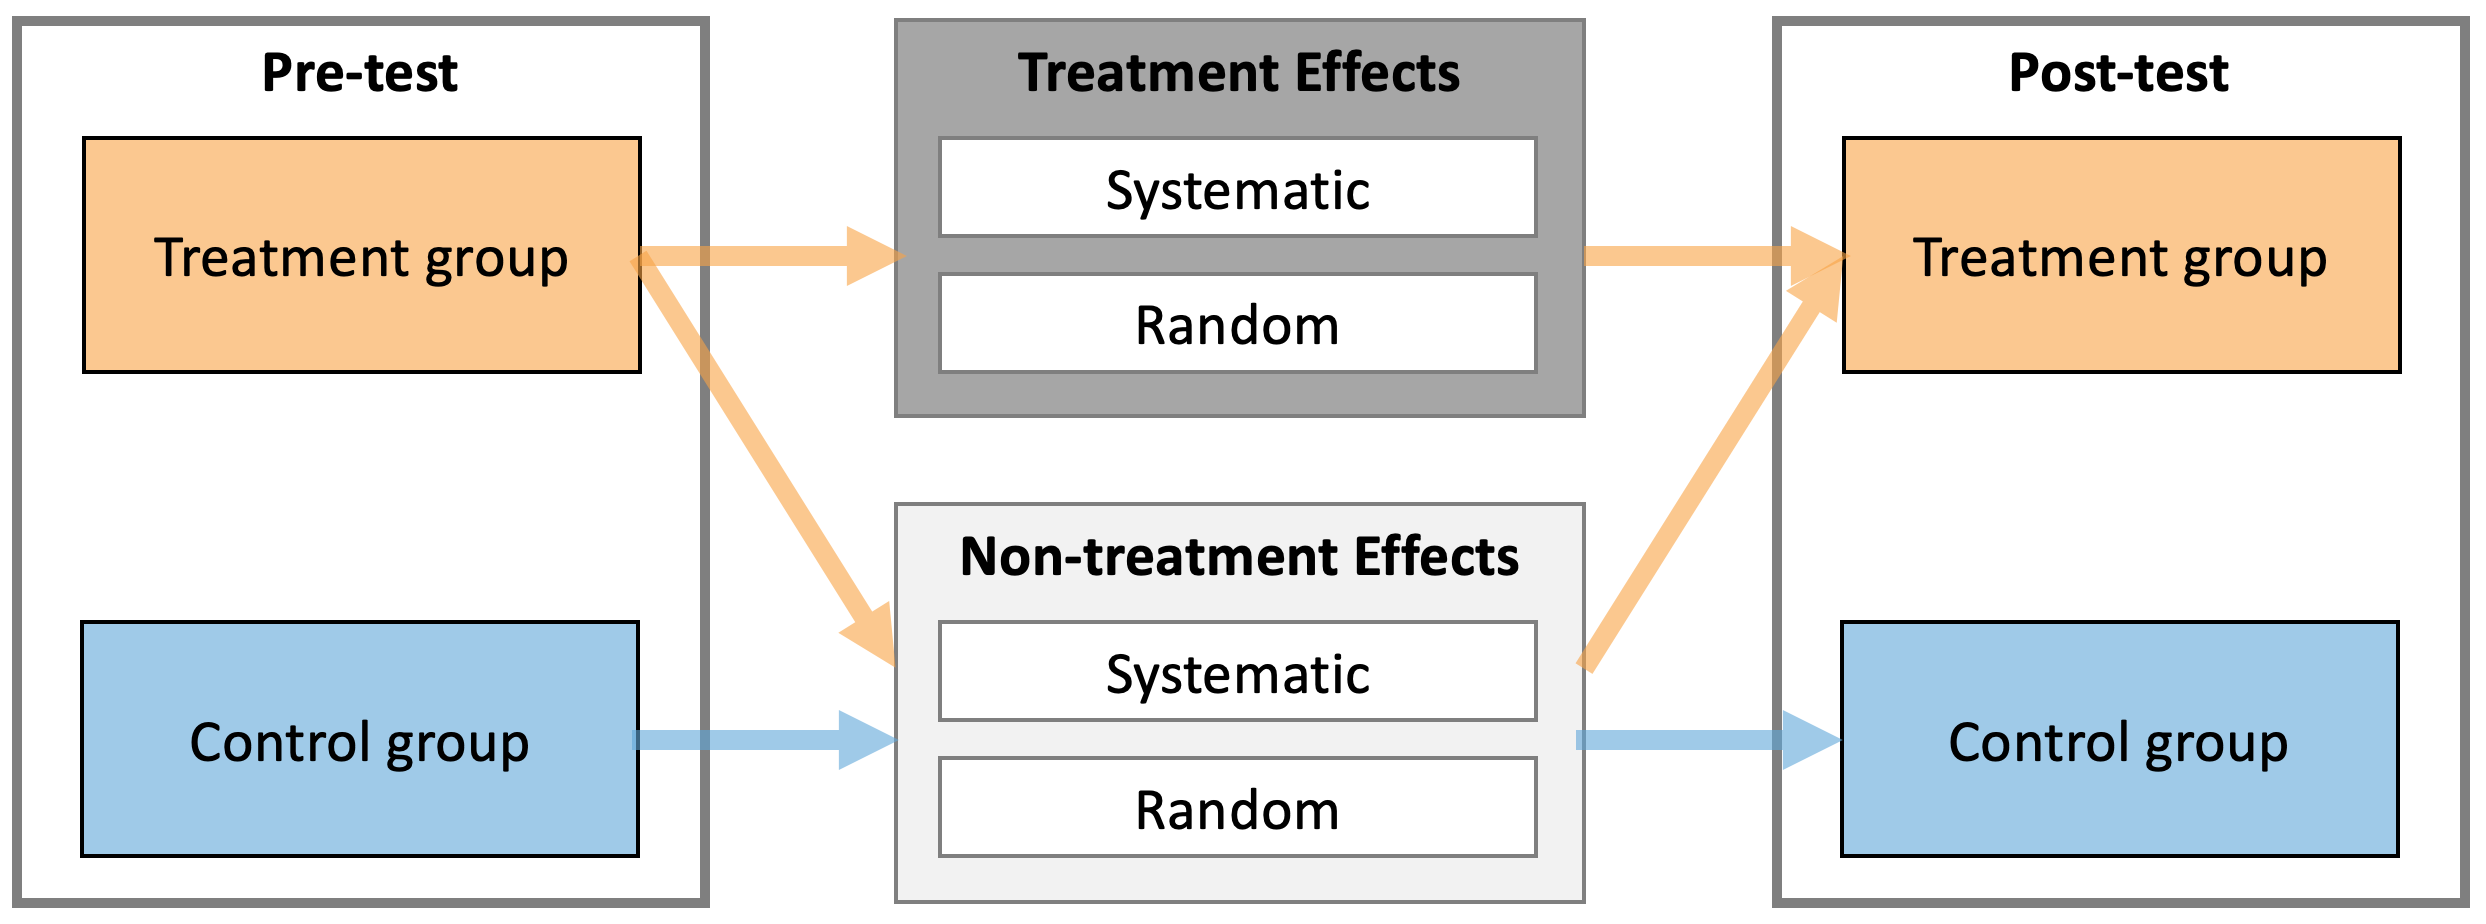
\includegraphics[width=1\linewidth]{figures/treatment-and-non-treatment-effects} 

}

\caption{\textbf{Treatment and Non-treatment effects of intervention.} Both treatment and non-treatment effects consists of two components: systematic and random. Treatment group experiences both treatment and non-treatment effects, while Control group experiences only non-treatment effects.}\label{fig:te-and-nte-diagram}
\end{figure}



The following equation captures the essence of estimating Treatment effects from Pre-test and Post-test scores in the Treatment and Control groups (Equation \eqref{eq:te-and-nte-equation}):

\begin{equation}
  \begin{split}
    Treatment_{post} &= Treatment_{pre} + Treatment \; Effect + NonTreatment \; Effect \\
    Control_{post} &= Control_{pre} + NonTreatment \; Effect \\
\\
    NonTreatment \; Effect &= Control_{post} - Control_{pre} \\
    Treatment \; Effect &= Treatment_{post} - Treatment_{pre} - NonTreatment \; Effect \\
\\
    Treatment \; Effect &= (Treatment_{post} - Treatment_{pre}) - (Control_{post} - Control_{pre}) \\
    Treatment \; Effect &= Treatment_{change} - Control_{change}
  \end{split}
  \label{eq:te-and-nte-equation}
\end{equation}

From the Equation \eqref{eq:te-and-nte-equation}, the differences between the changes in Treatment and Control groups can be interpreted as the estimate of the causal effect of the treatment. More precisely, average causal effect or expected causal effect represent systematic treatment effect. This is estimated using difference between \texttt{mean} Treatment change and \texttt{mean} Control change.

Table \ref{tab:rct-te-estimates} contains descriptive statistics of the change score differences. Panel C in the Figure \ref{fig:rct-paired-change} depicts distribution of the change scores and reflect the calculus in the Table \ref{tab:rct-te-estimates} graphically.



\begin{table}

\caption{\label{tab:rct-te-estimates}\textbf{Descriptive statistics of the change score differences}}
\centering
\resizebox{\linewidth}{!}{
\begin{tabular}[t]{rrrrrr}
\toprule
Mean difference (cm) & Cohen's d & Difference to SESOI & pLower diff & pEquivalent diff & pHigher diff\\
\midrule
7.9 & 9.56 & 1.58 & -0.03 & -0.79 & 0.82\\
\bottomrule
\end{tabular}}
\end{table}

\texttt{Cohen\textquotesingle{}s\ d} in the Table \ref{tab:rct-te-estimates} is calculated by using the Equation \eqref{eq:te-nte-cohen} and it estimates standardized difference between change scores in Treatment and the Control groups.

\begin{equation}
Cohen's\;d = \frac{mean_{treatment\; group \; change} - mean_{control\; group \;change}}{SD_{control\; group \; change}}
\label{eq:te-nte-cohen}
\end{equation}

Besides estimating systematic component of the treatment (i.e.~the difference between the mean change in Treatment and Control groups), we might be interested in estimating random component and proportions of lower, equivalent and higher effects compared to SESOI (\texttt{pLower}, \texttt{pEquivalent}, and \texttt{pHigher}). Unfortunately, differences in \texttt{pLower}, \texttt{pEquivalent}, and \texttt{pHigher} from Table \ref{tab:rct-te-estimates} don't answer this question, but rather the expected difference in proportions compared to Control (e.g.~the expected improvement of 0.82 in observing proportion of higher change outcomes compared to Control).

Since the changes in Treatment group are due both to the treatment and non-treatment effects (equation 29), the average treatment effect (systematic component) represents the difference between the \texttt{mean} changes in Treatment and Control groups (Table \ref{tab:rct-te-estimates}). In the same manner, the \texttt{variance} of the change scores in the Treatment group are due to the random component of the treatment and non-treatment effects. Assuming normal (Gaussian) distribution of the random components, the \emph{SD of the treatment effects} (\(SD_{TE}\))\footnote{Also referred to as \(SD_{IR}\) or standard deviation of the intervention responses (Will G. Hopkins \protect\hyperlink{ref-hopkinsIndividualResponsesMade2015}{2015}; Swinton et al. \protect\hyperlink{ref-swintonStatisticalFrameworkInterpret2018}{2018}). \(SD_{IR}\) or \(SD_{TE}\) represent estimate of treatment effect heterogeneity, also referred to as \emph{variable treatment effect} (VTE)} is estimated using the following Equation \eqref{eq:sd-te-equation}.

\begin{equation}
  \begin{split}
    \epsilon_{treatment \;group \;change} &= \epsilon_{treatment \; effect} + \epsilon_{nontreatment \; effect} \\
    \epsilon_{control \;group \;change} &= \epsilon_{nontreatment \; effect} \\
    \epsilon_{treatment \; effect} &= \epsilon_{treatment \;group \;change} - \epsilon_{control \;group \;change} \\
    \\
    \epsilon_{treatment \; effect}  &\sim \mathcal{N}(0,\,SD_{TE}) \\
    \epsilon_{nontreatment \; effect}  &\sim \mathcal{N}(0,\,SD_{NTE}) \\
    \epsilon_{treatment \;group \;change} &\sim \mathcal{N}(0,\,SD_{treatment \;group \;change}) \\
    \epsilon_{control \;group \;change} &\sim \mathcal{N}(0,\,SD_{control \;group \;change}) \\
    \\
    SD_{TE} &= \sqrt{SD_{treatment \;group \;change}^2 - SD_{control \;group \;change}^2}
  \end{split}
  \label{eq:sd-te-equation}
\end{equation}

This neat mathematical solution is due to assumption of Gaussian error, assumption that random treatment and non-treatment effects are equal across subjects (see \protect\hyperlink{ergodicity}{Ergodicity} section for more details about this assumption), and the use of squared errors. This is one beneficial property of using squared errors that I alluded to in the section \protect\hyperlink{cross-validation}{Cross-Validation} section.

Thus, the estimated parameters of the causal treatment effects in the underlying DGP are are summarized with the following Equation \eqref{eq:treatment-effects-estimates}. This treatment effect is graphically depicted in the Figure \ref{fig:te-effects}.

\begin{equation}
  \begin{split}
    Treatment \; effect &\sim \mathcal{N}(Mean_{TE},\,SD_{TE}) \\
    \\
    Mean_{TE} &= Mean_{treatment \;group \;change} - Mean_{control \;group \;change} \\ 
    \\
    SD_{TE} &= \sqrt{SD_{treatment \;group \;change}^2 - SD_{control \; group \; change}^2}
  \end{split}
  \label{eq:treatment-effects-estimates}
\end{equation}

\begin{figure}[!htb]

{\centering 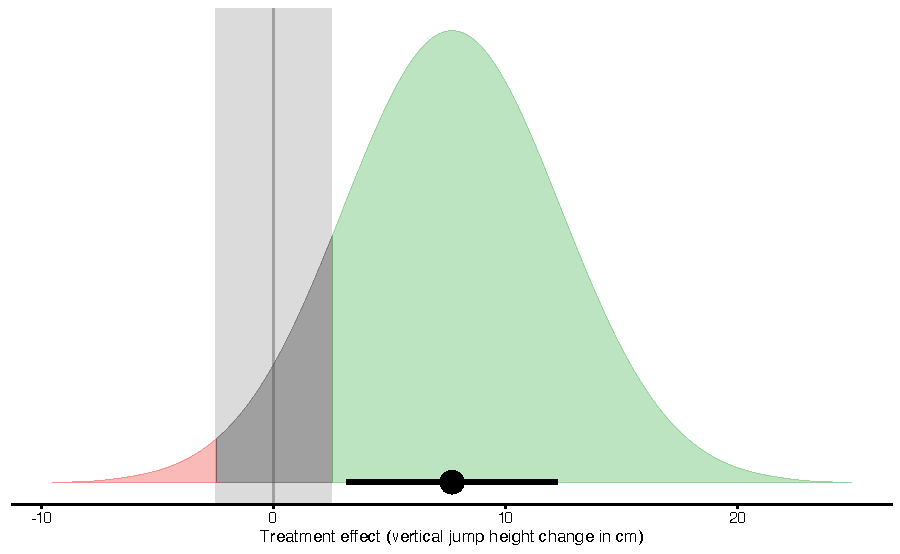
\includegraphics[width=0.9\linewidth]{04-Causal-inference_files/figure-latex/te-effects-1} 

}

\caption{\textbf{Graphical representation of the causal Treatment effect.} Green area indicates proportion of higher than SESOI treatment effects, red indicates proportion of negative and lower than SESOI treatment effects, and grey indicates treatment effects that are within SESOI. \texttt{Mean} of treatment effect distribution represents average (or expected) causal effect or systematic treatment effect. \texttt{SD} of treatment effect distribution represents random systematic effect or \(SD_{TE}\)}\label{fig:te-effects}
\end{figure}



Using SESOI, one can also estimate the proportion of lower, equivalent and higher changes (responses) caused by treatment. The estimates of the causal treatment effects, with accompanying proportions of responses are enlisted in the Table \ref{tab:te-effects-estimates}.



\begin{table}

\caption{\label{tab:te-effects-estimates}\textbf{Estimates of the causal treatment effects}}
\centering
\resizebox{\linewidth}{!}{
\begin{tabular}[t]{rrlrrrrr}
\toprule
Average causal effect (cm) & Random effect (cm) & SESOI (cm) & Average causal effect to SESOI & SESOI to random effect & pLower & pEquivalent & pHigher\\
\midrule
7.9 & 4.57 & ±2.5 & 1.58 & 1.09 & 0.01 & 0.11 & 0.88\\
\bottomrule
\end{tabular}}
\end{table}

Therefore, we can conclude that plyometric training over three months period, on top of the normal training, cause improvements in vertical jump height (in the sample collected; \emph{generalizations} beyond sample are discussed in the \protect\hyperlink{statistical-inference}{Statistical inference} section). The expected improvement (i.e.~average causal effect or systematic effect) is equal to 7.9cm, with 1, 11, and 88\% of athletes having lower, trivial and higher improvements.

\hypertarget{prediction-as-a-complement-to-causal-inference}{%
\section{Prediction as a complement to causal inference}\label{prediction-as-a-complement-to-causal-inference}}

In the previous section, RCT is analyzed using \emph{analysis of changes}. In this section, I will utilize linear regression model to analyze RCT data. There are multiple ways this could be done (J et al. \protect\hyperlink{ref-jDifferentWaysEstimate2018}{2018}) and deeper analysis is beyond the scope of this book (see also \href{https://www.fharrell.com/post/errmed/\#change}{Frank Harrell} post on the use of change scores). The aim of this section is to provide an introduction to \emph{model-based} and \emph{prediction-based} RCT analysis, as well as to demonstrate potential uses of PDP+ICE plots as tools for counterfactual analysis.

Analysis in the previous section can be represented using simple linear regression model (Equation \eqref{eq:simple-rct-change-regression}).

\begin{equation}
  \widehat{Change} = \hat{\beta_0} + \hat{\beta_1}Group
  \label{eq:simple-rct-change-regression}
\end{equation}

According to \href{https://www.fharrell.com/post/errmed/\#change}{Frank Harrell}, the use of change scores in the RCT analysis is problematic. Although this model definition (Equation \eqref{eq:simple-rct-change-regression}) will give us exactly the same results as obtained in the previous section, the use of change scores should be avoided. Thus, look at this example as \emph{training vehicle}. After this initial discussion, valid model representation will be used.

Since Group column is a string, how is Group column represented in the model? Group column needs to be \emph{dummy-coded}, using 0 for Control and 1 for Treatment (see Table \ref{tab:dummy-coded}).



\begin{table}

\caption{\label{tab:dummy-coded}\textbf{Dummy coding of the Group column to be used in linear regression model}}
\centering
\resizebox{\linewidth}{!}{
\begin{tabular}[t]{lrrrr}
\toprule
Athlete & groupTreatment & Pre-test (cm) & Post-test (cm) & Change (cm)\\
\midrule
Athlete 12 & 0 & 42.56 & 44.29 & 1.01\\
Athlete 28 & 0 & 47.06 & 47.98 & 0.55\\
Athlete 04 & 0 & 44.53 & 45.13 & 0.12\\
Athlete 02 & 0 & 49.63 & 48.86 & -0.01\\
Athlete 08 & 0 & 41.11 & 42.13 & -0.45\\
\addlinespace
Athlete 26 & 0 & 42.31 & 41.61 & -0.51\\
Athlete 06 & 0 & 45.96 & 45.70 & -0.52\\
Athlete 14 & 0 & 44.51 & 42.89 & -0.63\\
Athlete 18 & 0 & 42.57 & 42.15 & -0.74\\
Athlete 16 & 0 & 37.63 & 37.83 & -0.75\\
\addlinespace
Athlete 22 & 0 & 36.52 & 34.83 & -0.97\\
Athlete 24 & 0 & 40.15 & 39.88 & -1.03\\
Athlete 30 & 0 & 39.34 & 38.34 & -1.21\\
Athlete 20 & 0 & 38.94 & 36.97 & -1.72\\
Athlete 10 & 0 & 36.77 & 34.15 & -2.26\\
\addlinespace
Athlete 01 & 1 & 37.98 & 52.86 & 14.93\\
Athlete 27 & 1 & 44.79 & 58.50 & 13.43\\
Athlete 19 & 1 & 46.77 & 59.76 & 12.99\\
Athlete 25 & 1 & 38.90 & 49.58 & 10.81\\
Athlete 03 & 1 & 41.29 & 51.41 & 10.34\\
\addlinespace
Athlete 23 & 1 & 48.41 & 57.57 & 8.58\\
Athlete 17 & 1 & 44.81 & 51.41 & 7.85\\
Athlete 21 & 1 & 37.14 & 44.95 & 7.37\\
Athlete 15 & 1 & 46.69 & 52.73 & 6.14\\
Athlete 29 & 1 & 42.77 & 47.38 & 5.02\\
\addlinespace
Athlete 13 & 1 & 49.66 & 54.11 & 4.46\\
Athlete 05 & 1 & 37.92 & 41.63 & 3.78\\
Athlete 07 & 1 & 41.03 & 45.41 & 3.42\\
Athlete 11 & 1 & 45.27 & 46.72 & 1.82\\
Athlete 09 & 1 & 47.61 & 45.62 & -1.57\\
\bottomrule
\end{tabular}}
\end{table}

Estimated parameters for this linear model are enlisted in the Table \ref{tab:simple-rct-model-coef}



\begin{table}

\caption{\label{tab:simple-rct-model-coef}\textbf{Estimated linear regression parameters for the simple RCT model}}
\centering
\begin{tabular}[t]{rr}
\toprule
Intercept & groupTreatment\\
\midrule
-0.61 & 7.9\\
\bottomrule
\end{tabular}
\end{table}

Intercept in the Table \ref{tab:simple-rct-model-coef} represents the \texttt{mean} Change in the Control group, while \(\hat{\beta_1}\) (or slope, or \texttt{GroupTreatment} parameter) represents estimated average treatment effect (ATE) or average causal effect, since it represents the difference in the Change means between groups. For a reference please refer to Tables \ref{tab:rct-change} and \ref{tab:te-effects-estimates}.

Figure \ref{fig:simple-rct-model} depicts this model graphically.

\begin{figure}[!htb]

{\centering 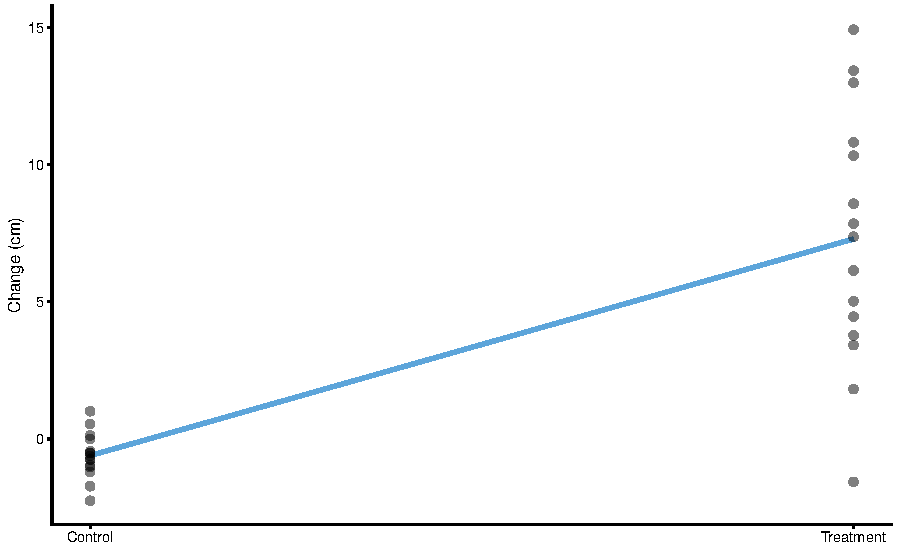
\includegraphics[width=0.9\linewidth]{04-Causal-inference_files/figure-latex/simple-rct-model-1} 

}

\caption{\textbf{Graphical representation of the simple linear regression model for the vertical jump RCT data}}\label{fig:simple-rct-model}
\end{figure}



Model residuals are depicted on Figure \ref{fig:simple-rct-model-ba}. Please note the \emph{clusters} of the data-points which indicate groups (they are color-coded).

\begin{figure}[!htb]

{\centering 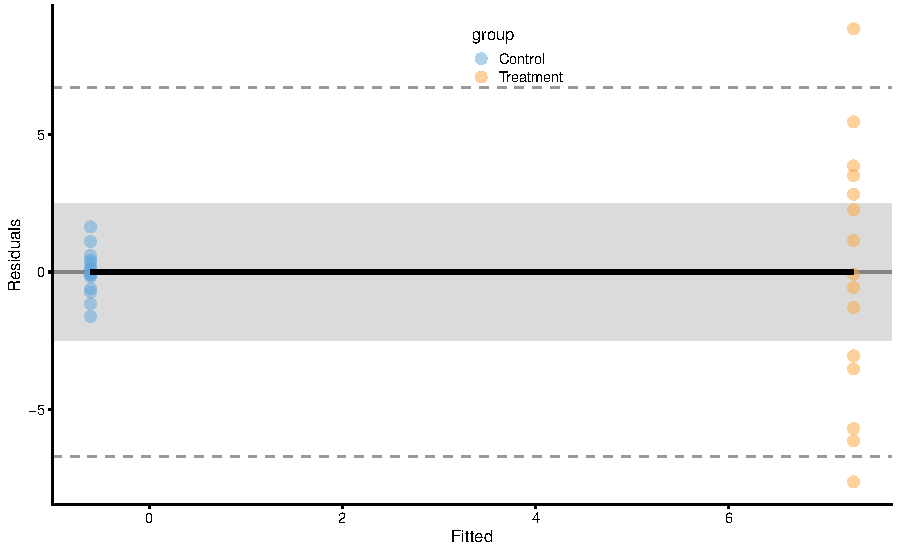
\includegraphics[width=0.9\linewidth]{04-Causal-inference_files/figure-latex/simple-rct-model-ba-1} 

}

\caption{\textbf{Model residuals using simple linear regression RCT model. }Grey band represents SESOI of ±2.5cm. Residuals are color coded; blue are Control group and orange are Treatment group.}\label{fig:simple-rct-model-ba}
\end{figure}



\texttt{SD} of the residuals for the Control group is equal to 0.83cm and for Treatment group is equal to 4.65cm. Please compare these estimates and estimated parameters from the Table \ref{tab:simple-rct-model-coef} with Table \ref{tab:rct-change} and Table \ref{tab:te-effects-estimates}. These estimates are identical since the model utilized (Equation \eqref{eq:simple-rct-change-regression}) is mathematically equivalent to the analysis done in the \protect\hyperlink{example-of-randomized-control-trial}{Example of randomized control trial} section.

As alluded in the introduction of this section, RCT analysis using change scores should be avoided. Valid way to analyze the RCT in this case is to use Post-test as the outcome, and Pre-test and Group as predictors. This can be easily understood graphically (Figure \ref{fig:ancova-rct-model}). On Figure \ref{fig:ancova-rct-model} each group (i.e.~Control and Treatment) is modeled separately.

\begin{figure}[!htb]

{\centering 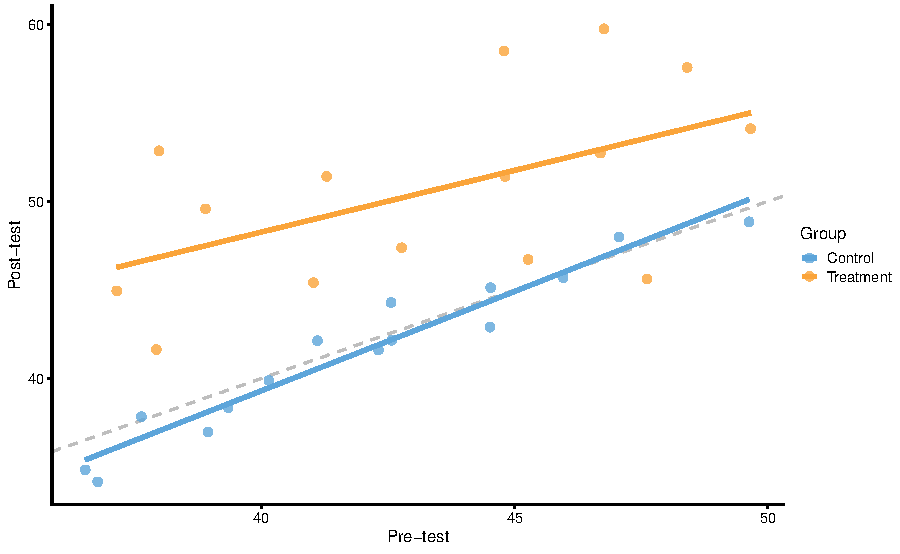
\includegraphics[width=0.9\linewidth]{04-Causal-inference_files/figure-latex/ancova-rct-model-1} 

}

\caption{\textbf{Graphical representation of the valid way to analyze RCT data.} Dashed line represent \emph{identity line}, where Post-test is equal to Pre-test (i.e., \emph{the no effect} line). The effect of treatment represents vertical distance between the Control and Treatment lines. This is easily grasped since the lines are almost perfectly parallel. If the lines are not parallel, that would imply there is \emph{interaction} between Group and Pre-test (i.e.~individuals with higher Pre-test scores shows higher or lower change).}\label{fig:ancova-rct-model}
\end{figure}



Figure \ref{fig:ancova-rct-model} also represents \emph{ANCOVA} (analysis of co-variance) design. Equation \eqref{eq:ancova-rct-change-regression} represent model definition where effects of Group (i.e., Treatment) are estimated by controlling the effects of the Pre-test.

\begin{equation}
  \widehat{Post} = \hat{\beta_0} + \hat{\beta_1}Group + \hat{\beta_2}Pre
  \label{eq:ancova-rct-change-regression}
\end{equation}

Estimated parameters for this linear model are enlisted in the Table \ref{tab:ancova-rct-model-coef}. Please note the similarity with the Table \ref{tab:simple-rct-model-coef}.



\begin{table}

\caption{\label{tab:ancova-rct-model-coef}\textbf{Estimated linear regression parameters for the ANCOVA RCT model (see Equation \eqref{eq:ancova-rct-change-regression})}}
\centering
\begin{tabular}[t]{rrr}
\toprule
Intercept & groupTreatment & Pre-test\\
\midrule
3.92 & 7.85 & 0.9\\
\bottomrule
\end{tabular}
\end{table}

Model residuals are depicted on Figure \ref{fig:ancova-rct-model-ba}. Please note the \emph{clusters} of the data-points which indicate groups.

\begin{figure}[!htb]

{\centering 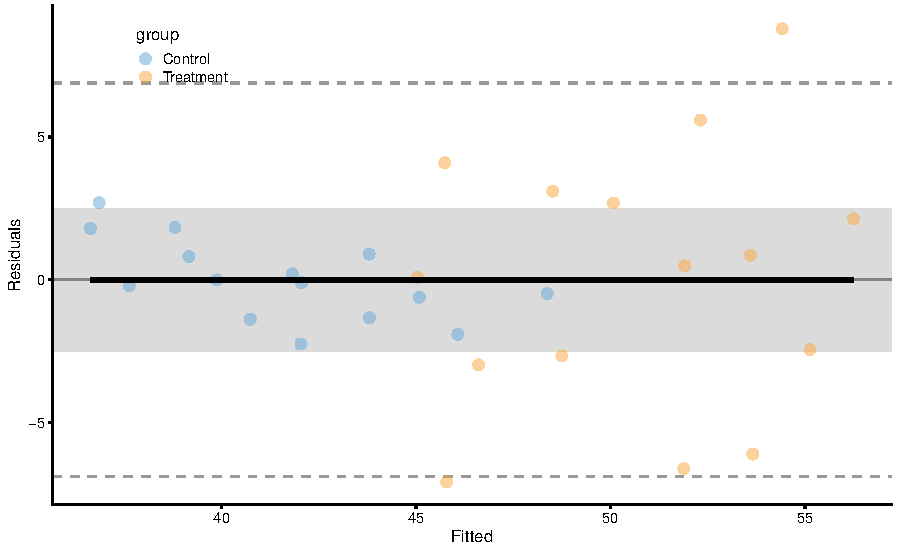
\includegraphics[width=0.9\linewidth]{04-Causal-inference_files/figure-latex/ancova-rct-model-ba-1} 

}

\caption{\textbf{Model residuals using ANCOVA RCT model. }Grey band represents SESOI of ±2.5cm. Residuals are color coded; blue are Control group and orange are Treatment group.}\label{fig:ancova-rct-model-ba}
\end{figure}



\texttt{SD} of the residuals for the Control group is equal to 1.43cm and for Treatment group is equal to 4.64cm. Please note the similarities with simple RCT model (i.e.~using Change score as outcome and Group as predictor).

As explained in the \protect\hyperlink{prediction}{Prediction} section, this model can be cross-validated. Predictive performance metrics using 10 repeats of 3 folds cross-validation are enlisted in the Table \ref{tab:ancova-rct-model-perf-metrics}. Since our RCT data has two groups (i.e.~Control and Treatment), cross-validation needs to be \emph{stratified}. This makes sure that each group has their own cross-validation folds, and that testing data size for each group is proportional to the group size. This avoids scenarios where most training or testing data comes from a single group (which is more probable if one group is larger).



\begin{table}

\caption{\label{tab:ancova-rct-model-perf-metrics}\textbf{Cross-validated predictive performance metrics for the ANCOVA RCT model}}
\centering
\resizebox{\linewidth}{!}{
\begin{tabular}[t]{lrrrrrrr}
\toprule
metric & training & training.pooled & testing.pooled & mean & SD & min & max\\
\midrule
MBE & 0.00 & 0.00 & -0.04 & -0.04 & 1.19 & -2.00 & 2.04\\
MAE & 2.41 & 2.37 & 2.69 & 2.69 & 0.55 & 1.68 & 4.39\\
RMSE & 3.31 & 3.24 & 3.68 & 3.62 & 0.68 & 2.28 & 5.28\\
PPER & 0.54 & 0.56 & 0.50 & 0.48 & 0.08 & 0.34 & 0.68\\
SESOI to RMSE & 1.51 & 1.54 & 1.36 & 1.43 & 0.27 & 0.95 & 2.19\\
\addlinespace
R-squared & 0.75 & 0.76 & 0.69 & 0.70 & 0.14 & 0.25 & 0.91\\
MinErr & -7.08 & -7.80 & -8.83 & -6.14 & 2.23 & -8.83 & -1.65\\
MaxErr & 8.80 & 9.93 & 10.75 & 5.95 & 2.87 & 1.35 & 10.75\\
MaxAbsErr & 8.80 & 9.93 & 10.75 & 7.91 & 1.59 & 3.78 & 10.75\\
\bottomrule
\end{tabular}}
\end{table}

From the Table \ref{tab:ancova-rct-model-perf-metrics} we can conclude, that although we have \emph{explained} the causal (or treatment) effects, predicting individual Post-test is not practically meaningful since the prediction error is too large (compared to SESOI). The take-home message is that high \emph{explanatory power} of the model doesn't doesn't automatically yield high predictive power (Shmueli \protect\hyperlink{ref-shmueliExplainPredict2010}{2010}). The selection of statistical analysis is thus related to the question asked. In my opinion, it would be insightful to complement causal estimates with prediction estimates. With the example above, we can predict the direction of the effect (using expected systematic change of 7.9cm and proportions of 1, 11, and 88\% for lower, trivial and higher change magnitudes), but we are unable to predict individual Post-test (or changes scores) within acceptable practical precision (using SESOI as an anchor). In other words, we know that the effect will be 88\% beneficial (i.e.~higher than SESOI), but we are not able to predict individual responses.

For the sake of completeness, Table \ref{tab:simple-rct-model-perf-metrics} contains performance metrics for the simple RCT model.



\begin{table}

\caption{\label{tab:simple-rct-model-perf-metrics}\textbf{Cross-validated predictive performance metrics for the simple RCT model}}
\centering
\resizebox{\linewidth}{!}{
\begin{tabular}[t]{lrrrrrrr}
\toprule
metric & training & training.pooled & testing.pooled & mean & SD & min & max\\
\midrule
MBE & 0.00 & 0.00 & 0.00 & 0.00 & 1.05 & -2.22 & 1.98\\
MAE & 2.16 & 2.14 & 2.30 & 2.30 & 0.48 & 1.33 & 3.44\\
RMSE & 3.22 & 3.19 & 3.41 & 3.35 & 0.66 & 2.02 & 4.53\\
PPER & 0.55 & 0.57 & 0.53 & 0.51 & 0.09 & 0.39 & 0.73\\
SESOI to RMSE & 1.55 & 1.57 & 1.47 & 1.56 & 0.35 & 1.10 & 2.48\\
\addlinespace
R-squared & 0.60 & 0.61 & 0.55 & 0.57 & 0.19 & -0.14 & 0.82\\
MinErr & -7.64 & -8.73 & -9.10 & -5.97 & 2.10 & -9.10 & -1.40\\
MaxErr & 8.86 & 9.84 & 10.33 & 5.67 & 3.05 & 0.59 & 10.33\\
MaxAbsErr & 8.86 & 9.84 & 10.33 & 7.69 & 1.62 & 3.78 & 10.33\\
\bottomrule
\end{tabular}}
\end{table}

\hypertarget{analysis-of-the-individual-residuals-responders-vs-non-responders}{%
\subsection{Analysis of the individual residuals: responders vs non-responders}\label{analysis-of-the-individual-residuals-responders-vs-non-responders}}

One particular use of the predictive analysis is in the identification of responders and non-responders to the treatment (Hecksteden et al. \protect\hyperlink{ref-heckstedenIndividualResponseExercise2015}{2015}, \protect\hyperlink{ref-heckstedenRepeatedTestingAssessment2018}{2018}; Will G. Hopkins \protect\hyperlink{ref-hopkinsIndividualResponsesMade2015}{2015}; Swinton et al. \protect\hyperlink{ref-swintonStatisticalFrameworkInterpret2018}{2018}). Common approach used in sport science (Will G Hopkins \protect\hyperlink{ref-hopkinsHowInterpretChanges2004}{2004}\protect\hyperlink{ref-hopkinsHowInterpretChanges2004}{a}), that I will name \emph{observed outcome approach} (further discussed in \protect\hyperlink{measurement-error}{Measurement error} chapter and second part of this book), uses known SESOI and \emph{measurement error} to estimate probability of lower, equivalent, and higher changes. In RCT, random non-treatment effect can be assumed to be due to measurement error. Figure \ref{fig:rct-responders} depicts individual \emph{adjusted change} (by deducting mean Control group change from observed change) with error bars representing \emph{smallest detectable change} (\texttt{SDC}). \texttt{SDC} is calculated by multiplying Control group change \texttt{SD} by 1.96 (to get upper and lower change levels containing 95\% of change distribution). This thus represent our \emph{uncertainty} in true treatment effect (using Control group as source of information about random effects).

\begin{figure}[!htb]

{\centering 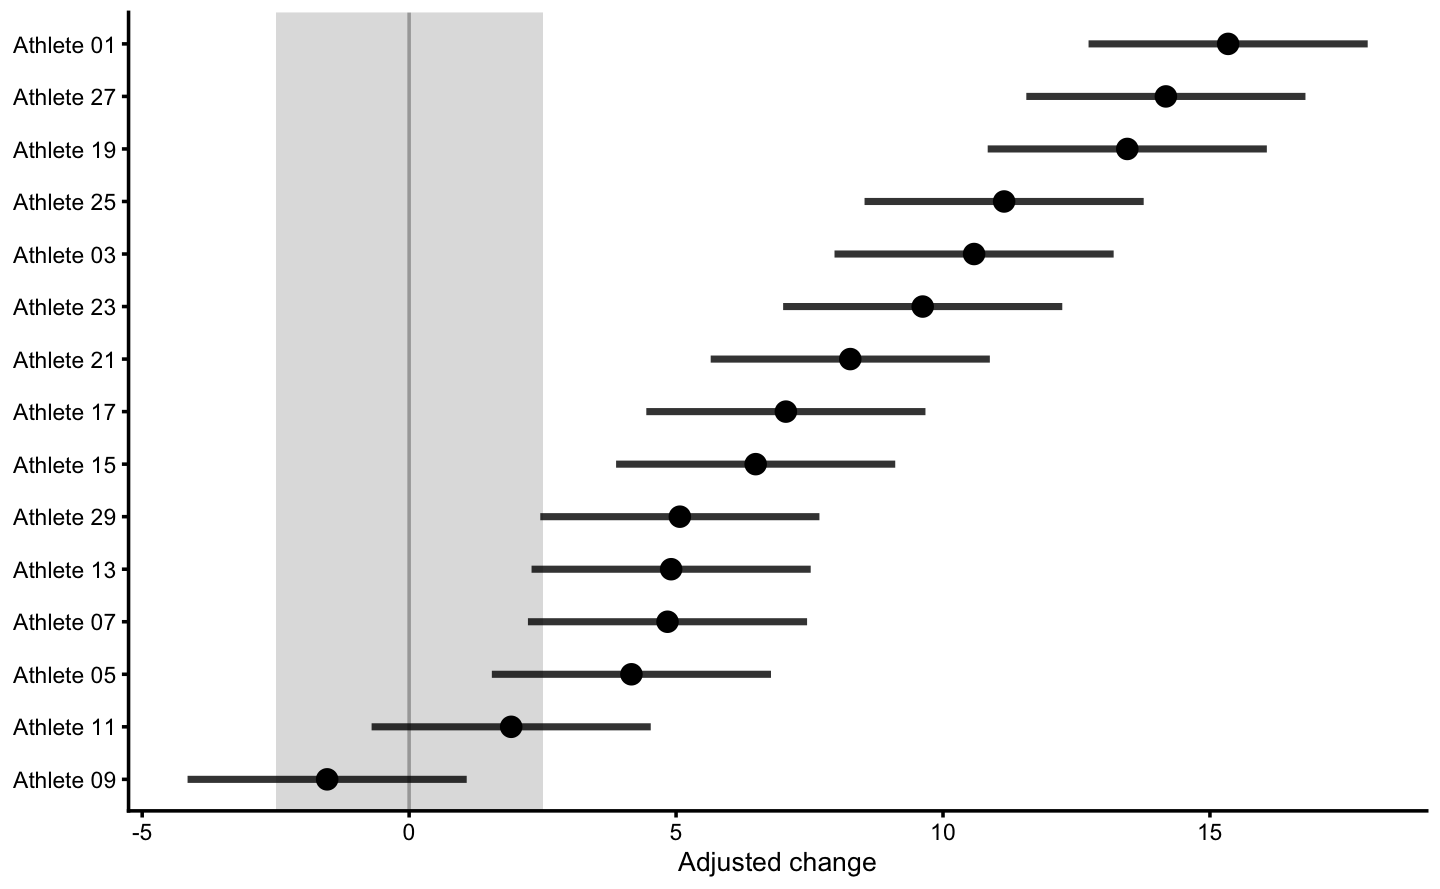
\includegraphics[width=0.9\linewidth]{04-Causal-inference_files/figure-latex/rct-responders-1} 

}

\caption{\textbf{Responses analysis for the Treatment group.} Change scores are adjusted by deducting Control group mean change. Error bars represent \emph{smallest detectable change} (SDC) that is calculated using \texttt{SD} of the Control group change scores multiplied by 1.96 (to get 95\% levels containing 95\% of the change distribution).}\label{fig:rct-responders}
\end{figure}



Using this approach, we can classify athletes with high probability of higher change score as responders, those with high probability of equivalent change score as non-responders, and finally those with high probability of lower change score as negative-responders. This approach is useful in figuring out who responded positively or negatively to a particular treatment, but it doesn't take into account information that might help explain the response (for example someone missing treatment session or having lower or higher treatment dose; see \protect\hyperlink{direct-and-indirect-effect-covariates-and-then-some}{Direct and indirect effect, covariates and then some} section). The topic is further discussed in \protect\hyperlink{measurement-error}{Measurement error} chapter and second part of this book.

Another approach, that I have termed \emph{residuals approach} or \emph{model-based approach} can be used to help identifying \emph{outliers} to intervention. To explain this approach, let's plot athletes' residuals (\(\hat{y_i} - y_i\)) against observed Post-test (\(y_i\)) (Figure \ref{fig:ancova-rct-subj-resid}) using ANCOVA RCT model.

\begin{figure}[!htb]

{\centering 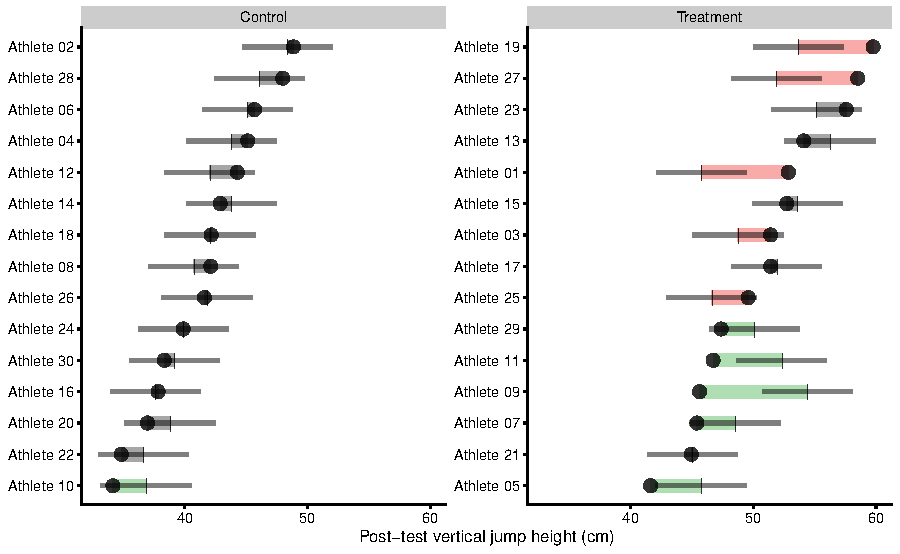
\includegraphics[width=0.9\linewidth]{04-Causal-inference_files/figure-latex/ancova-rct-subj-resid-1} 

}

\caption{\textbf{Observed Post-test in vertical jump for each athlete in the study.} Black dot indicate observed Post-test value; vertical line indicate model prediction; colored bar indicated the residual magnitude compared to defined SESOI (±2.5cm in this example): grey for equivalent magnitude, green for lower magnitude, and red for higher magnitude; horizontal error bar represents cross-validated \texttt{RMSE} (see Table \ref{tab:ancova-rct-model-perf-metrics}, \texttt{RMSE} metric, column \emph{testing.pooled}) and is used to indicate model predictive performance and uncertainty around model prediction graphically}\label{fig:ancova-rct-subj-resid}
\end{figure}



If we visualize simple model of RCT, using Change score as outcome and Group as predictor (see Figure \ref{fig:simple-rct-model}), the predictions for athletes in each group are identical (i.e.~the average change). This is depicted in Figure (Figure \ref{fig:simple-rct-subj-resid}).

\begin{figure}[!htb]

{\centering 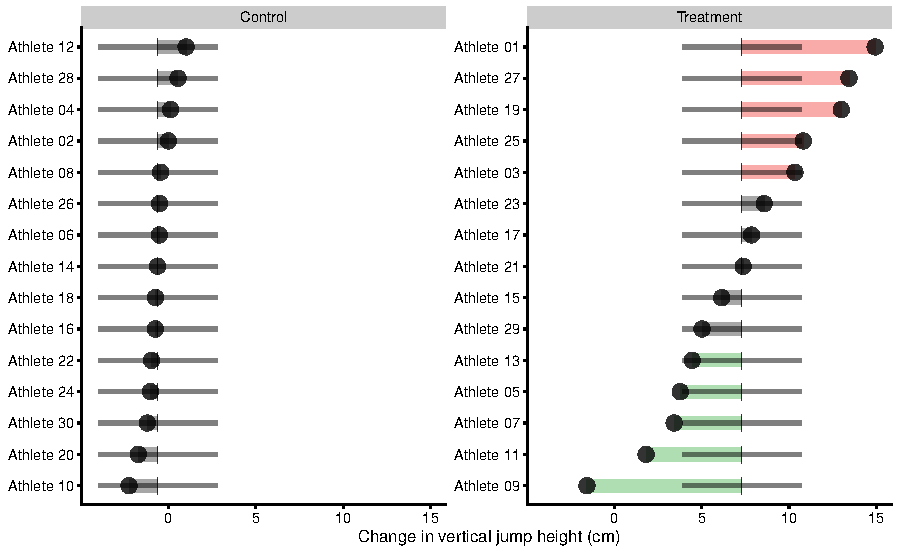
\includegraphics[width=0.9\linewidth]{04-Causal-inference_files/figure-latex/simple-rct-subj-resid-1} 

}

\caption{\textbf{Observed Change in vertical jump for each athlete in the study.} Black dot indicate observed Change value; vertical line indicate model prediction; colored bar indicated the residual magnitude compared to defined SESOI (±2.5cm in this example): grey for equivalent magnitude, green for lower magnitude, and red for higher magnitude; horizontal error bar represents cross-validated \texttt{RMSE} (see Table \ref{tab:simple-rct-model-perf-metrics}, \texttt{RMSE} metric, column \emph{testing.pooled}) and is used to indicate model predictive performance and uncertainty around model prediction graphically}\label{fig:simple-rct-subj-resid}
\end{figure}



More complex models (e.g.~ANCOVA RCT model in Figure \ref{fig:ancova-rct-subj-resid}), like the one utilized in \protect\hyperlink{direct-and-indirect-effect-covariates-and-then-some}{Direct and indirect effect, covariates and then some} section will have different predictions for each athlete.

Residuals approach uses observed scores and model predictions to indicate individuals who differ more or less than predicted by the model. If this difference between observed and predicted scores (or residual) is bigger than SESOI, this individual is \emph{flagged}. But before jumping to conclusions, I need to remind you that the predictive performance of this simple model is pretty bad (see Table \ref{tab:simple-rct-model-perf-metrics}). Thus, this type of analysis and visualization should be interpreted \emph{given} the model performance (which is indicated by horizontal line on the Figures \ref{fig:ancova-rct-subj-resid} and \ref{fig:simple-rct-subj-resid} which indicates cross-validated pooled testing \texttt{RMSE}; see Table \ref{tab:ancova-rct-model-perf-metrics}). I will utilize this method with a better model in the \protect\hyperlink{direct-and-indirect-effect-covariates-and-then-some}{Direct and indirect effect, covariates and then some} section that has much lower cross-validated \texttt{RMSE}. What is important to remember with this analysis is that athletes who showed lower or higher observation compared to what was predicted by the model are flagged with red or green color. As opposed to the observed outcome approach, a model-based prediction approach uses \emph{ceteris paribus} in estimating responders vs.~non-responders, or at least providing residuals for such a decision. For example, everything else being equal, based on predictor variables, the expected observation is higher or lower than the model prediction. This indicates that there might be something not-identified by predictive algorithm and thus needs to be flagged for a further analysis. But more about this in the \protect\hyperlink{direct-and-indirect-effect-covariates-and-then-some}{Direct and indirect effect, covariates and then some}.

Besides analyzing residuals in the training data-set, we can also check how model predicts for each individual within cross-validation using Bias-Variance decomposition (see \protect\hyperlink{bias-variance-decomposition-and-trade-off}{Bias-Variance decomposition and trade-off} section). Figure \ref{fig:ancova-rct-subj-bias-var} depicts prediction error (decomposed to Bias and Variance) for each athlete using ANCOVA RCT model.

\begin{figure}[!htb]

{\centering 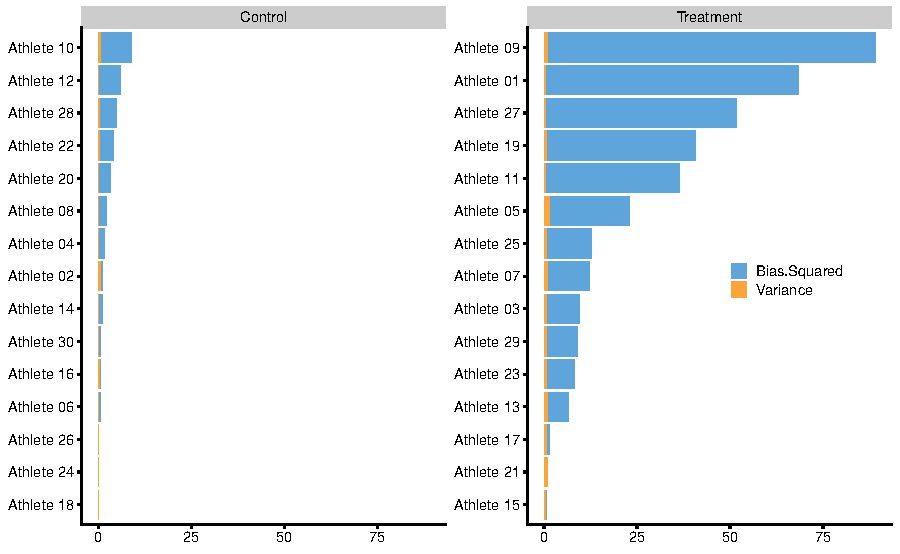
\includegraphics[width=0.9\linewidth]{04-Causal-inference_files/figure-latex/ancova-rct-subj-bias-var-1} 

}

\caption{\textbf{Bias-variance across 10 times repeated 3-fold cross-validation for each athlete. } This analysis can also be utilize to flag certain observations (i.e.~athlete in this case) that are troublesome for the predictive model}\label{fig:ancova-rct-subj-bias-var}
\end{figure}



These graphs will make much more sense when more predictive model is applied in the \protect\hyperlink{direct-and-indirect-effect-covariates-and-then-some}{Direct and indirect effect, covariates and then some} section.

\hypertarget{counterfactual-analysis-and-individual-treatment-effects}{%
\subsection{Counterfactual analysis and Individual Treatment Effects}\label{counterfactual-analysis-and-individual-treatment-effects}}

As explained, causal inference and explanatory modeling aim to understand, or at least to quantify the causal (or treatment) effects. This is done by elaborate and transparent control of the confounders and study designs. Predictive modelling on the other hand is interested in providing valid predictions on new or unseen data without assuming underlying DGP by treating it as a black-box. In certain scenarios, when confounders are controlled, predictive modelling can be interpreted causally (Zhao and Hastie \protect\hyperlink{ref-zhaoCausalInterpretationsBlackBox2019}{2019}). With observational studies, there is always a risk of not controlling all important confounders, but transparency of the causal model is there to be falsified and discussed openly (Gelman and Hennig \protect\hyperlink{ref-gelmanSubjectiveObjectiveStatistics2017}{2017}; Hernan \protect\hyperlink{ref-hernanCausalKnowledgePrerequisite2002}{2002}; Hernán \protect\hyperlink{ref-hernanCWordScientificEuphemisms2018}{2018}, \protect\hyperlink{ref-hernanDoesWaterKill2016}{2016}; Hernán and Taubman \protect\hyperlink{ref-hernanDoesObesityShorten2008}{2008}; Hernán, Hsu, and Healy \protect\hyperlink{ref-hernanSecondChanceGet2019}{2019}). Even with the RCTs, there might be uncertainties in applying the findings from the experiments to realistic settings (Gelman \protect\hyperlink{ref-gelmanCausalityStatisticalLearning2011}{2011}; Heckman \protect\hyperlink{ref-heckmanRejoinderResponseSobel2005}{2005}).

PDP and ICE plots are \emph{model-agnostic} tools for interpreting black-box models that can be used in causal interpretations only after the effort to define the causal structure with domain-specific expertise is taken into account. This approach can be used to estimate, based on the predictive model, counterfactual change and Post-test scores when athletes do not receive treatment (for the Treatment group), or when athletes receive treatment (for the Control group). This way potential outcomes are predicted.

To explain how this is done, let's again consider the Table \ref{tab:dummy-coded}. Changing the Group column (in this case \texttt{groupTreatment}) for every observation (athletes in this case) while keeping all other variables (i.e.~columns) the same, we can get a glimpse into causal effects of the treatment (assuming the model and the data are valid for such an inference). The prediction model utilized is ANCOVA RCT model.

In the Table \ref{tab:ancova-rct-counterfactual-group}, columns \texttt{Post-test\_0\ (cm)} and \texttt{Post-test\_1\ (cm)} indicate these counterfactual changes for which we are interested how the model predicts. These predictions are in the columns \texttt{Post-test\_0\ (cm)} and \texttt{Post-test\_1\ (cm)}.



\begin{table}

\caption{\label{tab:ancova-rct-counterfactual-group}\textbf{Counterfactual table used to check how the model predicts when Group changes}}
\centering
\resizebox{\linewidth}{!}{
\begin{tabular}[t]{lrrrrrrrr}
\toprule
Athlete & groupTreatment & Pre-test (cm) & Post-test (cm) & Change (cm) & groupTreatment\_0 & Post-test\_0 (cm) & groupTreatment\_1 & Post-test\_1 (cm)\\
\midrule
Athlete 12 & 0 & 42.56 & 44.29 & 1.01 & 0 & 42.04 & 1 & 49.89\\
Athlete 28 & 0 & 47.06 & 47.98 & 0.55 & 0 & 46.07 & 1 & 53.92\\
Athlete 04 & 0 & 44.53 & 45.13 & 0.12 & 0 & 43.80 & 1 & 51.65\\
Athlete 02 & 0 & 49.63 & 48.86 & -0.01 & 0 & 48.37 & 1 & 56.22\\
Athlete 08 & 0 & 41.11 & 42.13 & -0.45 & 0 & 40.74 & 1 & 48.59\\
\addlinespace
Athlete 26 & 0 & 42.31 & 41.61 & -0.51 & 0 & 41.82 & 1 & 49.67\\
Athlete 06 & 0 & 45.96 & 45.70 & -0.52 & 0 & 45.09 & 1 & 52.93\\
Athlete 14 & 0 & 44.51 & 42.89 & -0.63 & 0 & 43.79 & 1 & 51.64\\
Athlete 18 & 0 & 42.57 & 42.15 & -0.74 & 0 & 42.06 & 1 & 49.90\\
Athlete 16 & 0 & 37.63 & 37.83 & -0.75 & 0 & 37.63 & 1 & 45.47\\
\addlinespace
Athlete 22 & 0 & 36.52 & 34.83 & -0.97 & 0 & 36.63 & 1 & 44.48\\
Athlete 24 & 0 & 40.15 & 39.88 & -1.03 & 0 & 39.88 & 1 & 47.73\\
Athlete 30 & 0 & 39.34 & 38.34 & -1.21 & 0 & 39.16 & 1 & 47.01\\
Athlete 20 & 0 & 38.94 & 36.97 & -1.72 & 0 & 38.80 & 1 & 46.65\\
Athlete 10 & 0 & 36.77 & 34.15 & -2.26 & 0 & 36.85 & 1 & 44.70\\
\addlinespace
Athlete 01 & 1 & 37.98 & 52.86 & 14.93 & 0 & 37.94 & 1 & 45.79\\
Athlete 27 & 1 & 44.79 & 58.50 & 13.43 & 0 & 44.04 & 1 & 51.88\\
Athlete 19 & 1 & 46.77 & 59.76 & 12.99 & 0 & 45.81 & 1 & 53.66\\
Athlete 25 & 1 & 38.90 & 49.58 & 10.81 & 0 & 38.76 & 1 & 46.61\\
Athlete 03 & 1 & 41.29 & 51.41 & 10.34 & 0 & 40.90 & 1 & 48.75\\
\addlinespace
Athlete 23 & 1 & 48.41 & 57.57 & 8.58 & 0 & 47.28 & 1 & 55.13\\
Athlete 17 & 1 & 44.81 & 51.41 & 7.85 & 0 & 44.06 & 1 & 51.91\\
Athlete 21 & 1 & 37.14 & 44.95 & 7.37 & 0 & 37.19 & 1 & 45.04\\
Athlete 15 & 1 & 46.69 & 52.73 & 6.14 & 0 & 45.75 & 1 & 53.59\\
Athlete 29 & 1 & 42.77 & 47.38 & 5.02 & 0 & 42.23 & 1 & 50.08\\
\addlinespace
Athlete 13 & 1 & 49.66 & 54.11 & 4.46 & 0 & 48.40 & 1 & 56.25\\
Athlete 05 & 1 & 37.92 & 41.63 & 3.78 & 0 & 37.89 & 1 & 45.74\\
Athlete 07 & 1 & 41.03 & 45.41 & 3.42 & 0 & 40.67 & 1 & 48.52\\
Athlete 11 & 1 & 45.27 & 46.72 & 1.82 & 0 & 44.47 & 1 & 52.31\\
Athlete 09 & 1 & 47.61 & 45.62 & -1.57 & 0 & 46.57 & 1 & 54.42\\
\bottomrule
\end{tabular}}
\end{table}

If we depict these changes in the Group for every athlete, we will get the ICE graph. Average of these predictions gives us the PDP graph. Figure \ref{fig:ancova-rct-pdp-ice} depicts PDP and ICE for the Group variable. We will get back to this graph in the \protect\hyperlink{direct-and-indirect-effect-covariates-and-then-some}{Direct and indirect effect, covariates and then some} section.

\begin{figure}[!htb]

{\centering 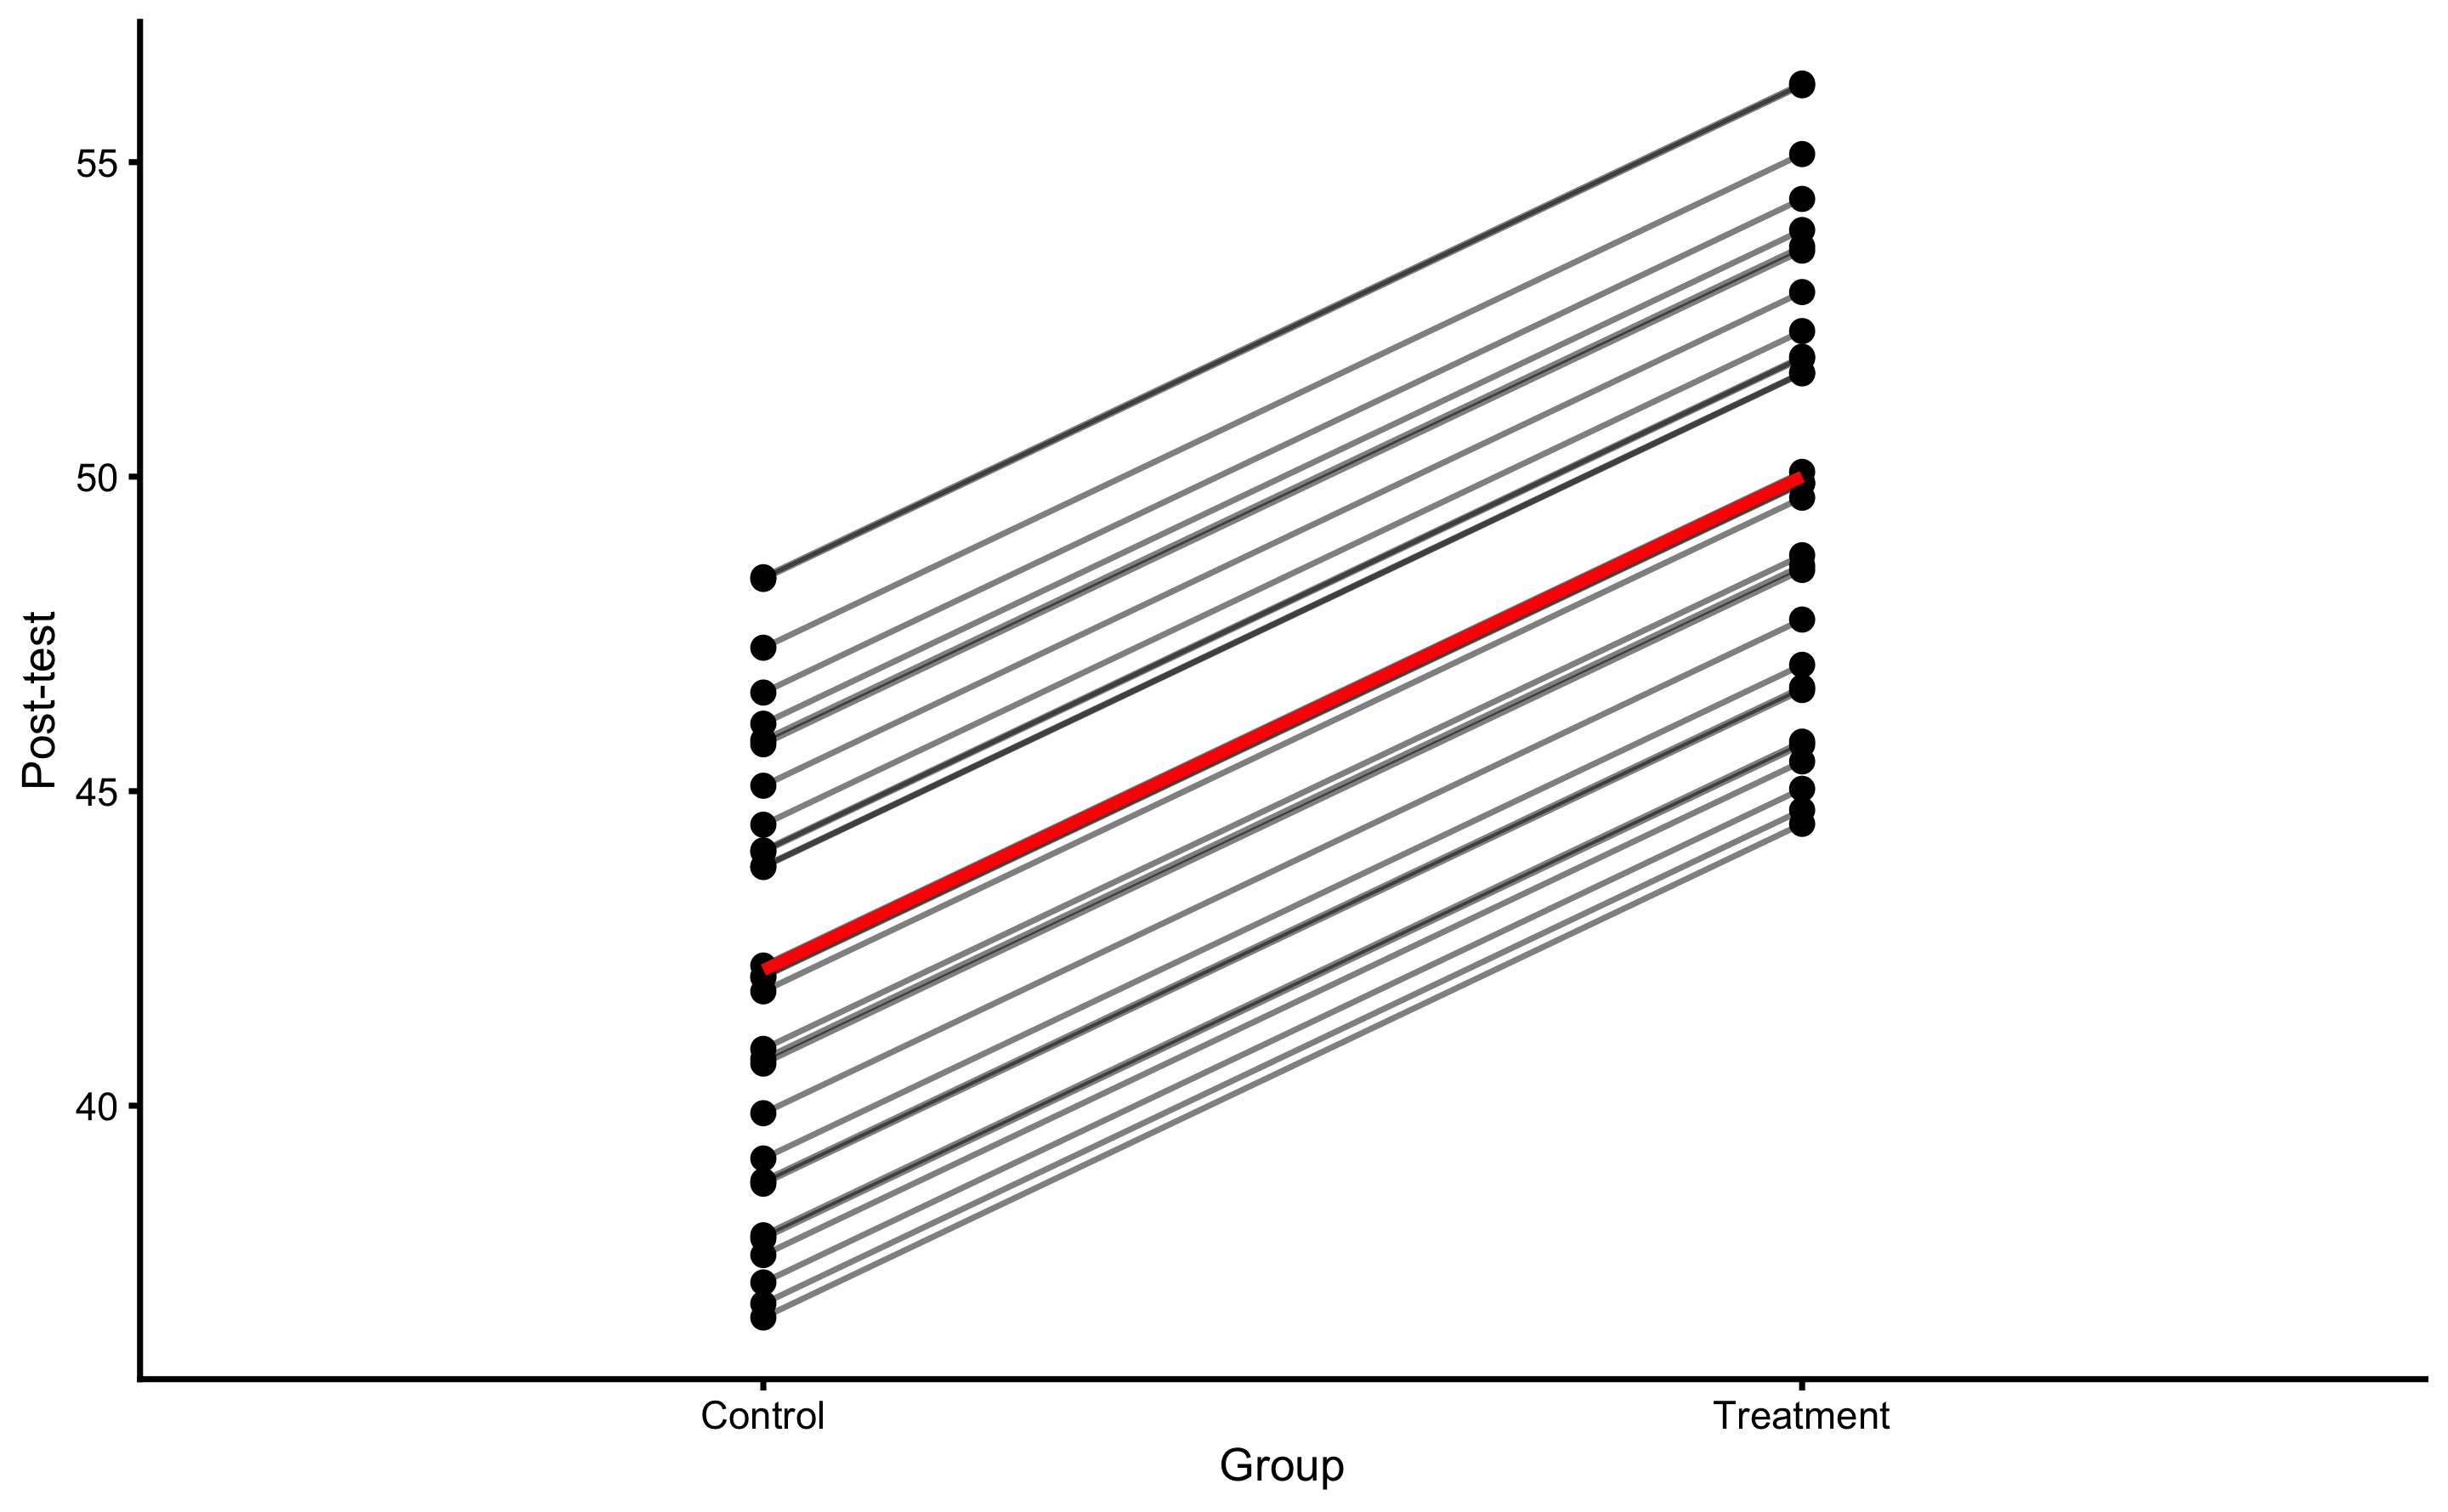
\includegraphics[width=0.9\linewidth]{04-Causal-inference_files/figure-latex/ancova-rct-pdp-ice-1} 

}

\caption{\textbf{PDP and ICE plot for Group variable using ANCOVA RCT model}}\label{fig:ancova-rct-pdp-ice}
\end{figure}



Besides PDP and ICE plot, we can also create a counterfactual plot for each athlete. For example, for the athletes in the Treatment group, we are interested how would the predicted Post-test \emph{change} (given model used) if they are in the Control group and \emph{vice versa} for the athletes from the Control group. This is done by \emph{flipping} ``Treatment'' and ``Control'' in the Group column and predicting Post-test using the trained model. Figure \ref{fig:ancova-rct-counterfactual-effects} depicts this visually for each athlete. Arrows represents predicted Change when \emph{flipping} the Group variable.

\begin{figure}[!htb]

{\centering 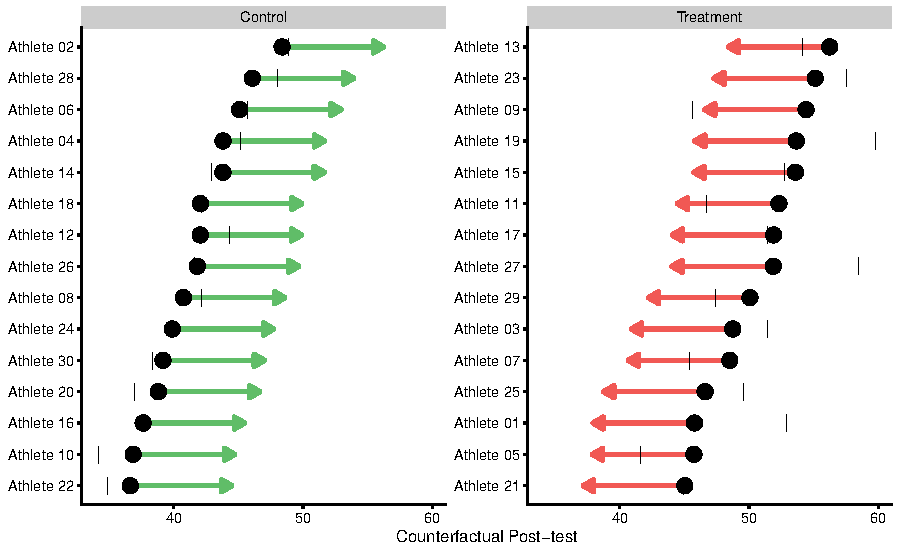
\includegraphics[width=0.9\linewidth]{04-Causal-inference_files/figure-latex/ancova-rct-counterfactual-effects-1} 

}

\caption{\textbf{Individual counterfactual prediction when the Group changes.} This way we can estimate model counterfactual predictions when the treatment changes (i.e.~Controls receive treatment, and Treatment doesn't receive treatment). Arrows thus represent model predicted \emph{Individual Treatment Effects} (pITE). Arrows are color coded based on the magnitude of the effect using defined SESOI (±2.5cm in this example): grey for equivalent magnitude, green for lower magnitude, and red for higher magnitude. Vertical line indicates observed Post-test scores.}\label{fig:ancova-rct-counterfactual-effects}
\end{figure}



This analysis allows us to estimate counterfactual \emph{individual causal (treatment) effects} (ITE) predicted by the model. These are indicated with the arrows on the Figure \ref{fig:ancova-rct-counterfactual-effects}. Mathematically, arrow width is calculates using the Equation \eqref{eq:ite-equation}.

\begin{equation}
  \widehat{ITE_i} = \widehat{y_{i}^{Group=Treatment}} - \widehat{y_{i}^{Group=Control}} 
  \label{eq:ite-equation}
\end{equation}

Since ANCOVA RCT model is used, which predicts average Group effect for every participant, estimated counterfactual ITEs are all the same and are equal to -7.85cm. Table \ref{tab:ancova-rct-pITE} contains all individual model predictions using ANCOVA RCT model.



\begin{table}

\caption{\label{tab:ancova-rct-pITE}\textbf{Individual model predictions using ANCOVA RCT model}}
\centering
\resizebox{\linewidth}{!}{
\begin{tabular}[t]{llrrrlrrl}
\toprule
subject & group & observed & predicted & residual & magnitude & counterfactual & pITE & pITE\_magnitude\\
\midrule
Athlete 12 & Control & 44.29 & 42.04 & -2.25 & Equivalent & 49.89 & 7.85 & Higher\\
Athlete 28 & Control & 47.98 & 46.07 & -1.91 & Equivalent & 53.92 & 7.85 & Higher\\
Athlete 04 & Control & 45.13 & 43.80 & -1.33 & Equivalent & 51.65 & 7.85 & Higher\\
Athlete 02 & Control & 48.86 & 48.37 & -0.48 & Equivalent & 56.22 & 7.85 & Higher\\
Athlete 08 & Control & 42.13 & 40.74 & -1.39 & Equivalent & 48.59 & 7.85 & Higher\\
\addlinespace
Athlete 26 & Control & 41.61 & 41.82 & 0.21 & Equivalent & 49.67 & 7.85 & Higher\\
Athlete 06 & Control & 45.70 & 45.09 & -0.61 & Equivalent & 52.93 & 7.85 & Higher\\
Athlete 14 & Control & 42.89 & 43.79 & 0.90 & Equivalent & 51.64 & 7.85 & Higher\\
Athlete 18 & Control & 42.15 & 42.06 & -0.10 & Equivalent & 49.90 & 7.85 & Higher\\
Athlete 16 & Control & 37.83 & 37.63 & -0.21 & Equivalent & 45.47 & 7.85 & Higher\\
\addlinespace
Athlete 22 & Control & 34.83 & 36.63 & 1.80 & Equivalent & 44.48 & 7.85 & Higher\\
Athlete 24 & Control & 39.88 & 39.88 & 0.00 & Equivalent & 47.73 & 7.85 & Higher\\
Athlete 30 & Control & 38.34 & 39.16 & 0.82 & Equivalent & 47.01 & 7.85 & Higher\\
Athlete 20 & Control & 36.97 & 38.80 & 1.84 & Equivalent & 46.65 & 7.85 & Higher\\
Athlete 10 & Control & 34.15 & 36.85 & 2.70 & Higher & 44.70 & 7.85 & Higher\\
\addlinespace
Athlete 01 & Treatment & 52.86 & 45.79 & -7.08 & Lower & 37.94 & -7.85 & Lower\\
Athlete 27 & Treatment & 58.50 & 51.88 & -6.62 & Lower & 44.04 & -7.85 & Lower\\
Athlete 19 & Treatment & 59.76 & 53.66 & -6.10 & Lower & 45.81 & -7.85 & Lower\\
Athlete 25 & Treatment & 49.58 & 46.61 & -2.98 & Lower & 38.76 & -7.85 & Lower\\
Athlete 03 & Treatment & 51.41 & 48.75 & -2.66 & Lower & 40.90 & -7.85 & Lower\\
\addlinespace
Athlete 23 & Treatment & 57.57 & 55.13 & -2.44 & Equivalent & 47.28 & -7.85 & Lower\\
Athlete 17 & Treatment & 51.41 & 51.91 & 0.49 & Equivalent & 44.06 & -7.85 & Lower\\
Athlete 21 & Treatment & 44.95 & 45.04 & 0.09 & Equivalent & 37.19 & -7.85 & Lower\\
Athlete 15 & Treatment & 52.73 & 53.59 & 0.86 & Equivalent & 45.75 & -7.85 & Lower\\
Athlete 29 & Treatment & 47.38 & 50.08 & 2.69 & Higher & 42.23 & -7.85 & Lower\\
\addlinespace
Athlete 13 & Treatment & 54.11 & 56.25 & 2.14 & Equivalent & 48.40 & -7.85 & Lower\\
Athlete 05 & Treatment & 41.63 & 45.74 & 4.11 & Higher & 37.89 & -7.85 & Lower\\
Athlete 07 & Treatment & 45.41 & 48.52 & 3.11 & Higher & 40.67 & -7.85 & Lower\\
Athlete 11 & Treatment & 46.72 & 52.31 & 5.59 & Higher & 44.47 & -7.85 & Lower\\
Athlete 09 & Treatment & 45.62 & 54.42 & 8.80 & Higher & 46.57 & -7.85 & Lower\\
\bottomrule
\end{tabular}}
\end{table}

PDP and ICE plots, as well as individual treatment effects plots (and estimates) can be very valuable tool in visualizing the causal effects, which are appropriate in this case since we are analyzing RCT data. But we need to be very wary when using them with the observational data and giving them causal interpretation.

\hypertarget{direct-and-indirect-effect-covariates-and-then-some}{%
\subsection{Direct and indirect effect, covariates and then some}\label{direct-and-indirect-effect-covariates-and-then-some}}

In the previous RCT example, we have assumed \emph{binary} treatment (either plyometric training is done or not), whereas in real life there can be nuances in the treatment, particularly in volume of jumps performed, making the treatment continuous rather than binary variable. This way, we are interested in the effects of number of jumps on the changes in vertical jump height.

There could also be \emph{hidden variables} involved that \emph{moderate} and \emph{mediate} the effects of the treatment\footnote{Using the randomization in the RCT it is assumed that these hidden variables are equally distributed, and that there is no \emph{selection bias} involved.}. For example, the higher someone jumps in the Pre-test, the lower the change in the Post-test (i.e.~it is harder to improve vertical jump height). Or, the stronger someone is in the Pre-test (measured using relative back squat 1RM) the more potentiated the effects of the plyometrics are. All these are needed expert subject-matter knowledge, required to understand the underlying DGP (and thus to avoid introducing bias in causal analyses; see Lübke et al. (\protect\hyperlink{ref-lubkeWhyWeShould2020}{2020})). With such causal structure, we do not have \emph{direct treatment effect} (plyometric --\textgreater{} change in vertical jump) only anymore, but moderated and mediated, or \emph{indirect effects} estimated using the \emph{interactions} in the regression models.

To explain these concepts, let's assume that that besides Pre-test and Post-test scores in our RCT study, we have also measured Back squat relative 1RMs since we believed that strength of the individual will moderate the effects of the plyometric treatment. This data is enlisted in the Table \ref{tab:rct-data-with-squat}. Squat 1RM in this case represent characteristic of the subject, or a \emph{covariate}. Additional covariates (not considered here) might include gender, experience, height, weight and so forth.

\begin{table}

\caption{\label{tab:rct-data-with-squat}\textbf{Randomized control trial data but now with 1RM strength covariate}}
\centering
\resizebox{\linewidth}{!}{
\begin{tabular}[t]{lrlrrr}
\toprule
Athlete & Squat 1RM & Group & Pre-test (cm) & Post-test (cm) & Change (cm)\\
\midrule
Athlete 12 & 1.53 & Control & 42.56 & 44.29 & 1.01\\
Athlete 28 & 1.59 & Control & 47.06 & 47.98 & 0.55\\
Athlete 04 & 1.49 & Control & 44.53 & 45.13 & 0.12\\
Athlete 02 & 1.31 & Control & 49.63 & 48.86 & -0.01\\
Athlete 08 & 1.77 & Control & 41.11 & 42.13 & -0.45\\
\addlinespace
Athlete 26 & 1.34 & Control & 42.31 & 41.61 & -0.51\\
Athlete 06 & 1.33 & Control & 45.96 & 45.70 & -0.52\\
Athlete 14 & 2.03 & Control & 44.51 & 42.89 & -0.63\\
Athlete 18 & 1.21 & Control & 42.57 & 42.15 & -0.74\\
Athlete 16 & 1.91 & Control & 37.63 & 37.83 & -0.75\\
\addlinespace
Athlete 22 & 1.49 & Control & 36.52 & 34.83 & -0.97\\
Athlete 24 & 1.37 & Control & 40.15 & 39.88 & -1.03\\
Athlete 30 & 1.04 & Control & 39.34 & 38.34 & -1.21\\
Athlete 20 & 1.58 & Control & 38.94 & 36.97 & -1.72\\
Athlete 10 & 1.67 & Control & 36.77 & 34.15 & -2.26\\
\addlinespace
Athlete 01 & 2.05 & Treatment & 37.98 & 52.86 & 14.93\\
Athlete 27 & 2.05 & Treatment & 44.79 & 58.50 & 13.43\\
Athlete 19 & 1.87 & Treatment & 46.77 & 59.76 & 12.99\\
Athlete 25 & 1.97 & Treatment & 38.90 & 49.58 & 10.81\\
Athlete 03 & 1.79 & Treatment & 41.29 & 51.41 & 10.34\\
\addlinespace
Athlete 23 & 1.44 & Treatment & 48.41 & 57.57 & 8.58\\
Athlete 17 & 1.21 & Treatment & 44.81 & 51.41 & 7.85\\
Athlete 21 & 1.49 & Treatment & 37.14 & 44.95 & 7.37\\
Athlete 15 & 1.43 & Treatment & 46.69 & 52.73 & 6.14\\
Athlete 29 & 1.22 & Treatment & 42.77 & 47.38 & 5.02\\
\addlinespace
Athlete 13 & 1.18 & Treatment & 49.66 & 54.11 & 4.46\\
Athlete 05 & 1.15 & Treatment & 37.92 & 41.63 & 3.78\\
Athlete 07 & 1.21 & Treatment & 41.03 & 45.41 & 3.42\\
Athlete 11 & 0.86 & Treatment & 45.27 & 46.72 & 1.82\\
Athlete 09 & 0.69 & Treatment & 47.61 & 45.62 & -1.57\\
\bottomrule
\end{tabular}}
\end{table}



Since the individual are randomized into Treatment and Control groups, we expect that there is no difference between Squat 1RM betweem them. Figure \ref{fig:rct-squat} demonstrates that there is no difference between groups.

\begin{figure}[!htb]

{\centering 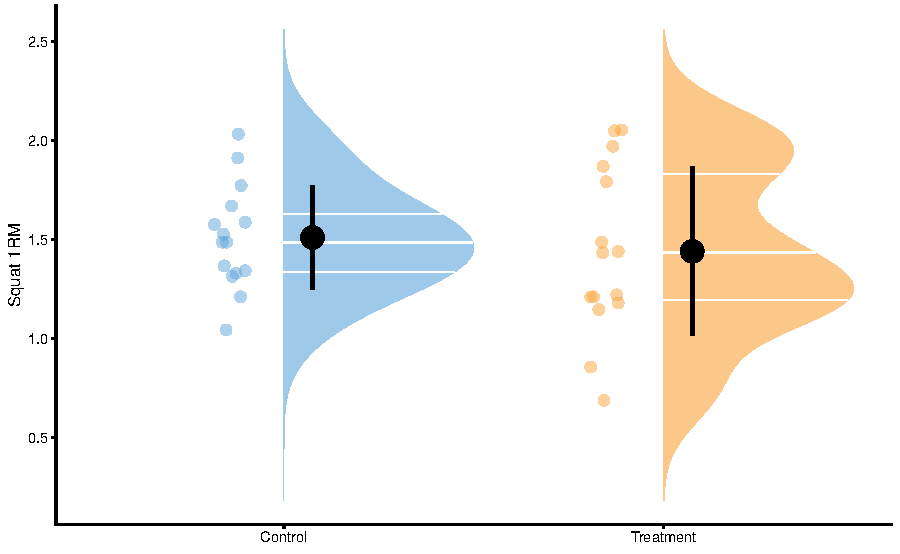
\includegraphics[width=0.9\linewidth]{04-Causal-inference_files/figure-latex/rct-squat-1} 

}

\caption{\textbf{Squat 1RM scores for Control and Treatment groups. } Since athletes are randomized, we expect them to be similar (i.e.~no selection bias involved)}\label{fig:rct-squat}
\end{figure}



Before modeling this RCT data, let's check visually the relationship between Pre-test and Change (panel A), Squat 1RM and Change (panel B), and Pre-test and Squat 1RM (panel C) (Figure \ref{fig:rct-change-relationships}).

\begin{figure}[!htb]

{\centering 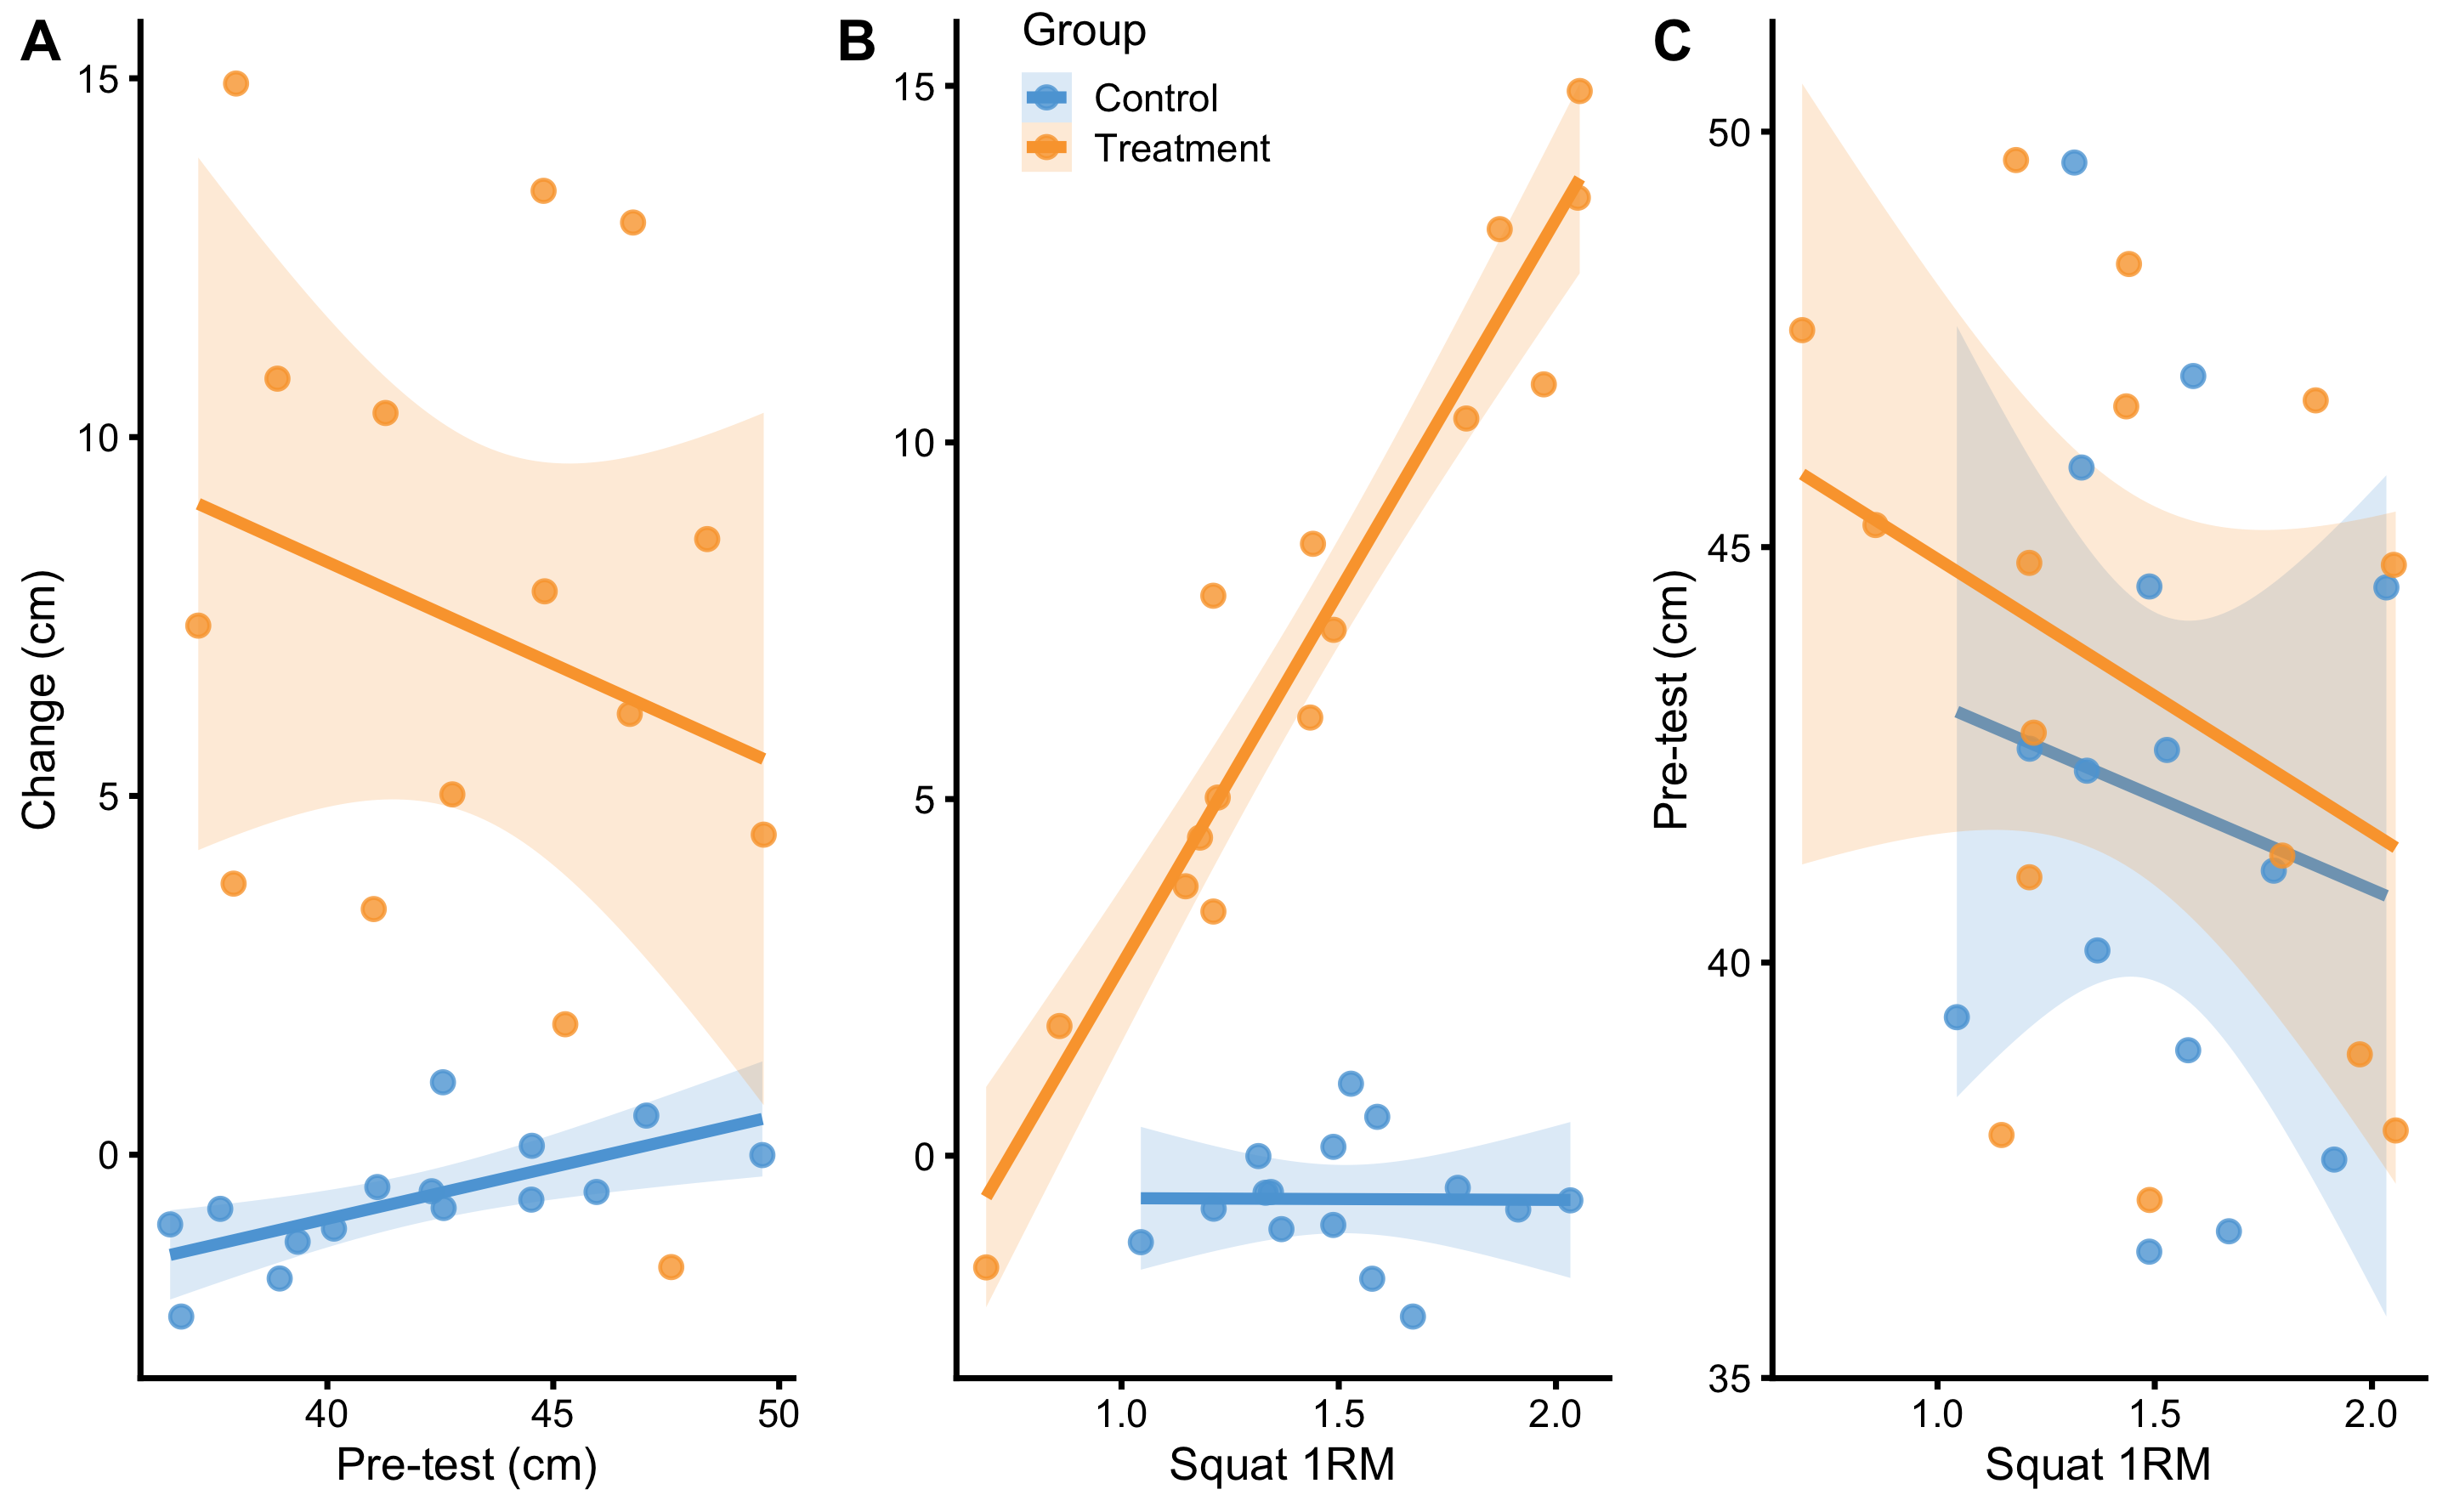
\includegraphics[width=0.9\linewidth]{04-Causal-inference_files/figure-latex/rct-change-relationships-1} 

}

\caption{\textbf{Relationship between predictors. A. } Relationship between Pre-test and Change scores. Lines indicate linear regression model and are used to indicate relationship and interaction. Colored area represent \emph{95\% confidence intervals} (see \protect\hyperlink{statistical-inference}{Statistical inference} section for more information). If there is no interaction between Pre-test and Change score, the lines would be parallel. As can be seen with the Treatment group, it seems that individuals with higher Pre-test demonstrates lower Change, and \emph{vice versa} for the Control group. But if we check the confidence interval area, these are due to random chance. \textbf{B.} Relationship between Squat 1RM and Change scores. Visual analysis indicates that individuals in the Treatment group with the higher Squat 1RM demonstrates higher changes after the training intervention. \textbf{C.} Relationship between Squat 1RM and Pre-test predictors. It seems that, in both groups, athletes with higher Squat 1RM scores have lower Pre-test values. Checking confidence interval areas, this relationship is due to random chance.}\label{fig:rct-change-relationships}
\end{figure}



As can be seen from the Figure \ref{fig:rct-change-relationships}, there seems to be some \emph{interaction} between Squat 1RM and Change. Other panels indicate that there might be some relationship (i.e.~\emph{interaction}), but \emph{95\% confidence intervals} around the regression lines indicate that these are due to \emph{random chance} (see \protect\hyperlink{statistical-inference}{Statistical inference} chapter for more info; for now you do not need to understand this concept).

What does interaction mean? If we check the panel C in the Figure \ref{fig:rct-change-relationships}, interaction refers to change in regression line slopes. If the Group regression lines are parallel, then the distance between them is due to effect of treatment (i.e.~direct or \emph{main} effect of treatment). Since they are not parallel, it means that Squat 1RM and treatment interact: the higher the Squat 1RM for the Treatment group, the higher the Change, while that is not the case for the Control group. Mathematically, interaction is a simple multiplication between two predictors, as cab be seen in the Table \ref{tab:rct-interaction}.



\begin{table}

\caption{\label{tab:rct-interaction}\textbf{RCT data with interaction between Group and Squat 1RM}}
\centering
\resizebox{\linewidth}{!}{
\begin{tabular}[t]{lrrrrr}
\toprule
Athlete & groupTreatment & Squat 1RM & groupTreatment:Squat 1RM & Pre-test (cm) & Change (cm)\\
\midrule
Athlete 12 & 0 & 1.53 & 0.00 & 42.56 & 1.01\\
Athlete 28 & 0 & 1.59 & 0.00 & 47.06 & 0.55\\
Athlete 04 & 0 & 1.49 & 0.00 & 44.53 & 0.12\\
Athlete 02 & 0 & 1.31 & 0.00 & 49.63 & -0.01\\
Athlete 08 & 0 & 1.77 & 0.00 & 41.11 & -0.45\\
\addlinespace
Athlete 26 & 0 & 1.34 & 0.00 & 42.31 & -0.51\\
Athlete 06 & 0 & 1.33 & 0.00 & 45.96 & -0.52\\
Athlete 14 & 0 & 2.03 & 0.00 & 44.51 & -0.63\\
Athlete 18 & 0 & 1.21 & 0.00 & 42.57 & -0.74\\
Athlete 16 & 0 & 1.91 & 0.00 & 37.63 & -0.75\\
\addlinespace
Athlete 22 & 0 & 1.49 & 0.00 & 36.52 & -0.97\\
Athlete 24 & 0 & 1.37 & 0.00 & 40.15 & -1.03\\
Athlete 30 & 0 & 1.04 & 0.00 & 39.34 & -1.21\\
Athlete 20 & 0 & 1.58 & 0.00 & 38.94 & -1.72\\
Athlete 10 & 0 & 1.67 & 0.00 & 36.77 & -2.26\\
\addlinespace
Athlete 01 & 1 & 2.05 & 2.05 & 37.98 & 14.93\\
Athlete 27 & 1 & 2.05 & 2.05 & 44.79 & 13.43\\
Athlete 19 & 1 & 1.87 & 1.87 & 46.77 & 12.99\\
Athlete 25 & 1 & 1.97 & 1.97 & 38.90 & 10.81\\
Athlete 03 & 1 & 1.79 & 1.79 & 41.29 & 10.34\\
\addlinespace
Athlete 23 & 1 & 1.44 & 1.44 & 48.41 & 8.58\\
Athlete 17 & 1 & 1.21 & 1.21 & 44.81 & 7.85\\
Athlete 21 & 1 & 1.49 & 1.49 & 37.14 & 7.37\\
Athlete 15 & 1 & 1.43 & 1.43 & 46.69 & 6.14\\
Athlete 29 & 1 & 1.22 & 1.22 & 42.77 & 5.02\\
\addlinespace
Athlete 13 & 1 & 1.18 & 1.18 & 49.66 & 4.46\\
Athlete 05 & 1 & 1.15 & 1.15 & 37.92 & 3.78\\
Athlete 07 & 1 & 1.21 & 1.21 & 41.03 & 3.42\\
Athlete 11 & 1 & 0.86 & 0.86 & 45.27 & 1.82\\
Athlete 09 & 1 & 0.69 & 0.69 & 47.61 & -1.57\\
\bottomrule
\end{tabular}}
\end{table}

But as already alluded, the use of Change scores should be avoided. Let's see this exact graphs, but using Post-test (Figure \ref{fig:rct-post-test-relationships}) as our variable of interest (i.e.~outcome variable).

\begin{figure}[!htb]

{\centering 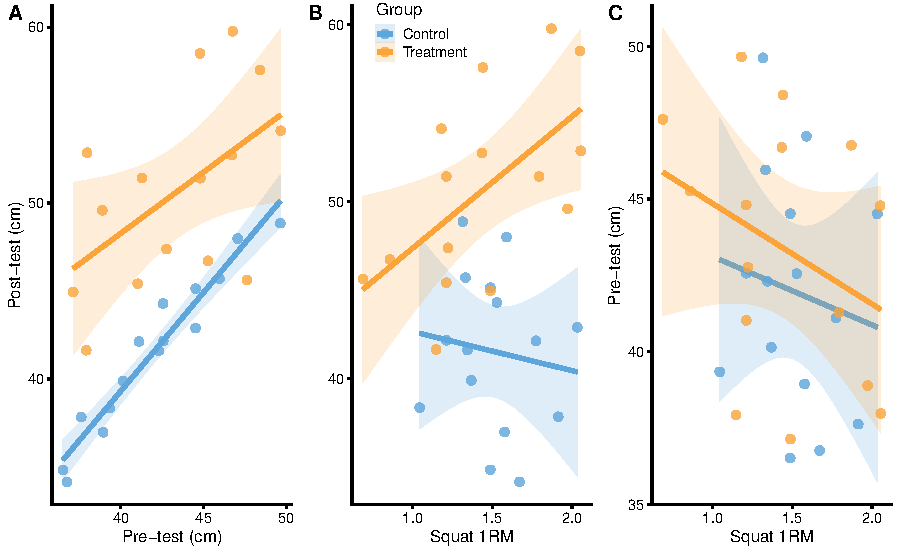
\includegraphics[width=0.9\linewidth]{04-Causal-inference_files/figure-latex/rct-post-test-relationships-1} 

}

\caption{\textbf{Relationship between predictors. A. } Relationship between Pre-test and Post-test scores. Lines indicate linear regression model and are used to indicate relationship and interaction. Colored area represent \emph{95\% confidence intervals} (see \protect\hyperlink{statistical-inference}{Statistical inference} section for more information). If there is no interaction between Pre-test and Post-test score, the lines would be parallel. As can be seen on the figure, there doesn't seem to be interaction involved. \textbf{B.} Relationship between Squat 1RM and Post-test scores. Visual analysis indicates that individuals in the Treatment group with the higher Squat 1RM demonstrates higher Post-test scores after the training intervention. \textbf{C.} Relationship between Squat 1RM and Pre-test predictors. It seems that, in both groups, athletes with higher Squat 1RM scores have lower Pre-test values. Checking confidence interval areas, this relationship is due to random chance.}\label{fig:rct-post-test-relationships}
\end{figure}



Let's apply linear regression model to these predictors. The parameters we are going to estimate are enlisted in the linear Equation \eqref{eq:rct-interaction-equation}.

\begin{equation}
  \widehat{Post} = \hat{\beta_0} + \hat{\beta_1}Group +  \hat{\beta_2}Pre + \hat{\beta_3}Squat\:1RM + \hat{\beta_4}Group:Squat\:1RM 
  \label{eq:rct-interaction-equation}
\end{equation}

Estimated parameters for this linear model with interaction are enlisted in the Table \ref{tab:rct-interaction-model-coef}.



\begin{table}

\caption{\label{tab:rct-interaction-model-coef}\textbf{Estimated linear regression parameters for the RCT model with interaction between Group and Squat 1RM}}
\centering
\resizebox{\linewidth}{!}{
\begin{tabular}[t]{rrrrr}
\toprule
Intercept & groupTreatment & Pre-test & Squat 1RM & Group:Squat 1RM\\
\midrule
-5.21 & -8.03 & 1.1 & 0.26 & 10.82\\
\bottomrule
\end{tabular}}
\end{table}

If we check the estimated coefficient for the group Treatment in the Table \ref{tab:rct-interaction-model-coef}, which is equal to -8.03, can we conclude that this is the whole effect of treatment (i.e.~plyometric treatment)? Luckily no! This coefficient represents \emph{direct treatment effect}, but there are \emph{indirect treatment effects} due to Squat 1RM and interaction between Squat 1RM and Group. This also assumes that we have not introduced bias in treatment effect estimation by \emph{adjusting} (or by \emph{not adjusting}) for covariates that we should not adjust for (or \emph{vice versa}; for great applied paper please refer to Lübke et al. (\protect\hyperlink{ref-lubkeWhyWeShould2020}{2020})).

Figure \ref{fig:rct-interaction-resid} depicts residuals of the RCT model with interactions.

\begin{figure}[!htb]

{\centering 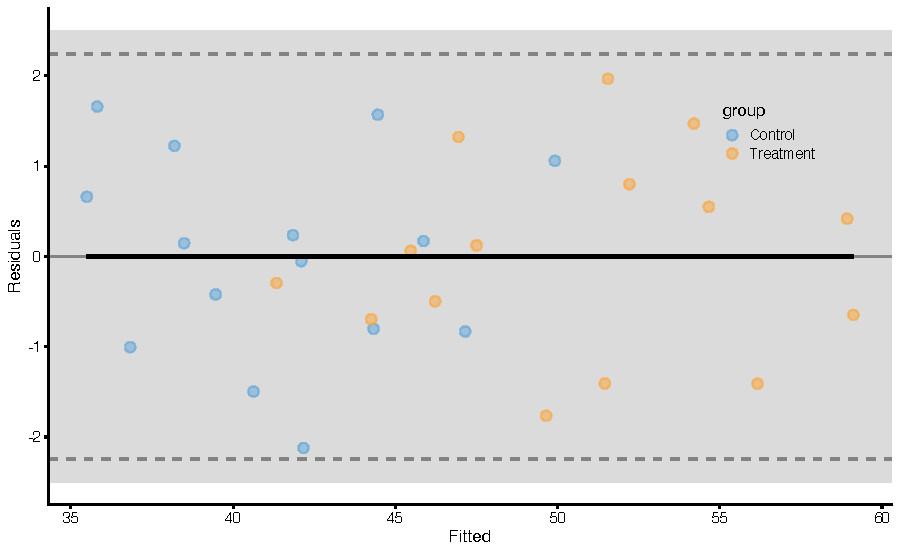
\includegraphics[width=0.9\linewidth]{04-Causal-inference_files/figure-latex/rct-interaction-resid-1} 

}

\caption{\textbf{Residuals of the linear regression RCT model with interaction. }Grey band on both panels represents SESOI of ±2.5cm}\label{fig:rct-interaction-resid}
\end{figure}



As opposed to the Figures \ref{fig:simple-rct-model-ba} and \ref{fig:ancova-rct-model-ba}, we can quickly see that this model have almost all residuals in the SESOI band. Table \ref{tab:interaction-rct-model-perf-metrics} contains cross-validated model performance (using the same 10 repeats of 3 folds cross-validation splits as used in the simple and ANCOVA RCT models).



\begin{table}

\caption{\label{tab:interaction-rct-model-perf-metrics}\textbf{Cross-validated predictive performance metrics for the RCT model with interaction}}
\centering
\resizebox{\linewidth}{!}{
\begin{tabular}[t]{lrrrrrrr}
\toprule
metric & training & training.pooled & testing.pooled & mean & SD & min & max\\
\midrule
MBE & 0.00 & 0.00 & 0.07 & 0.07 & 0.61 & -1.40 & 1.18\\
MAE & 0.90 & 0.81 & 1.19 & 1.19 & 0.25 & 0.75 & 1.76\\
RMSE & 1.08 & 1.00 & 1.46 & 1.43 & 0.27 & 0.89 & 1.99\\
PPER & 0.97 & 0.99 & 0.91 & 0.87 & 0.06 & 0.74 & 0.97\\
SESOI to RMSE & 4.64 & 5.02 & 3.43 & 3.61 & 0.73 & 2.52 & 5.61\\
\addlinespace
R-squared & 0.97 & 0.98 & 0.95 & 0.95 & 0.02 & 0.88 & 0.98\\
MinErr & -2.12 & -2.40 & -2.72 & -1.90 & 0.58 & -2.72 & -0.76\\
MaxErr & 1.97 & 2.12 & 3.15 & 2.27 & 0.80 & 0.32 & 3.15\\
MaxAbsErr & 2.12 & 2.40 & 3.15 & 2.57 & 0.42 & 1.65 & 3.15\\
\bottomrule
\end{tabular}}
\end{table}

As expected, predictive performance metrics are now much better. Let's inspect the athlete's residuals (Figure \ref{fig:interaction-rct-subj-resid}).

\begin{figure}[!htb]

{\centering 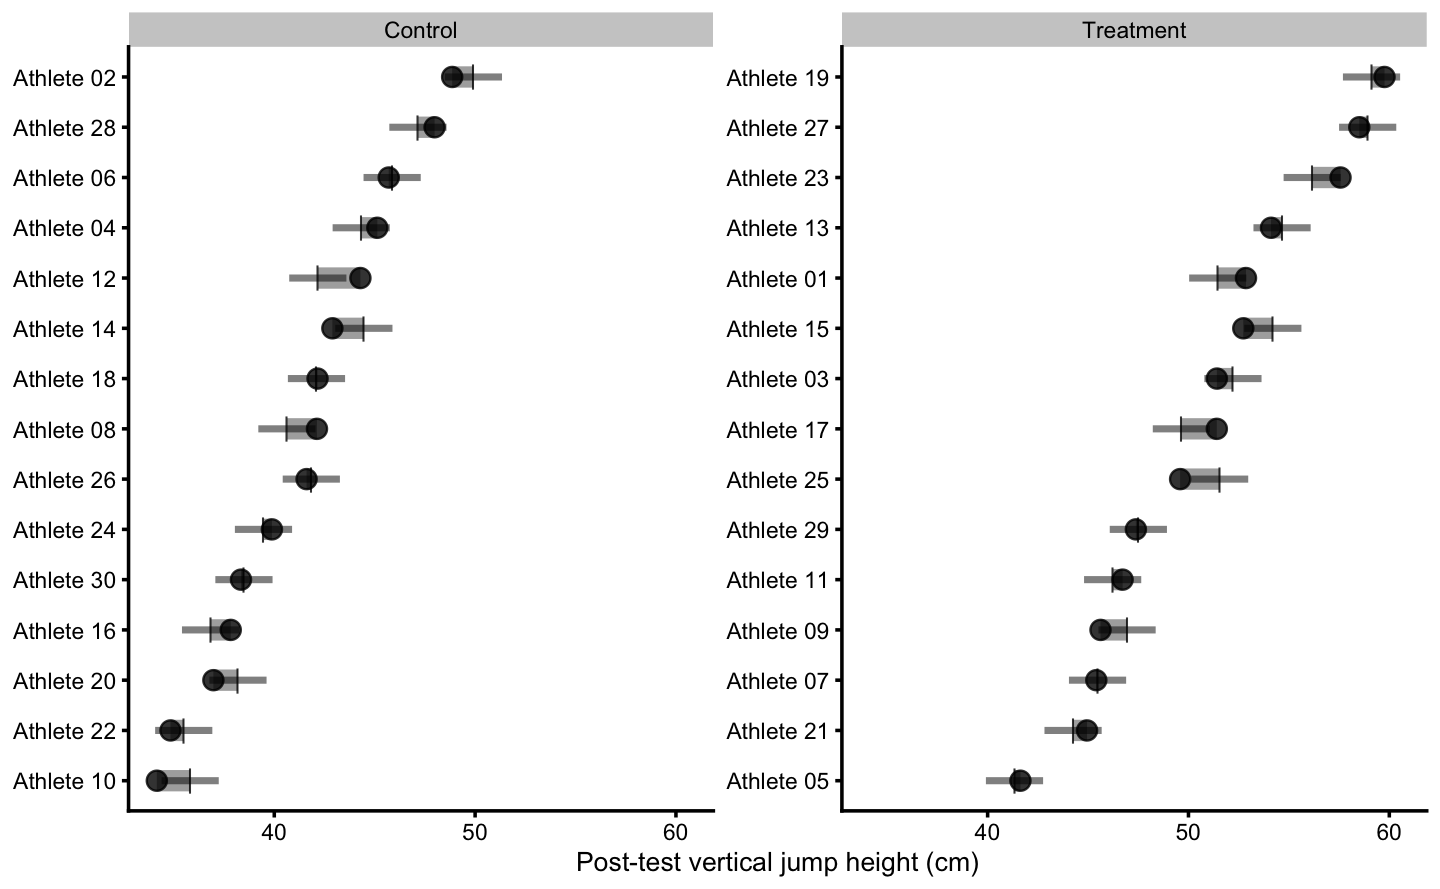
\includegraphics[width=0.9\linewidth]{04-Causal-inference_files/figure-latex/interaction-rct-subj-resid-1} 

}

\caption{\textbf{Observed Post-test in vertical jump for each athlete in the study.} Black dot indicate observed Post-test; vertical line indicate model prediction; colored bar indicated the residual magnitude compared to defined SESOI (±2.5cm in this example): grey for equivalent magnitude, green for lower magnitude, and red for higher magnitude; horizontal error bar represents cross-validated \texttt{RMSE} (see Table \ref{tab:interaction-rct-model-perf-metrics}, \texttt{RMSE} metric, column \emph{testing.pooled}) and is used to indicate visually model predictive performance and uncertainty around model prediction}\label{fig:interaction-rct-subj-resid}
\end{figure}



If we compare residuals from the simple model (Figure \ref{fig:simple-rct-subj-resid}) and ANCOVA RCT model (Figure \ref{fig:ancova-rct-subj-resid}), in RCT model with interactions the residuals are much smaller, indicating better prediction. You can also see that model predictions differ, as opposed to simple model that predicted same Change values for all athletes in the Control and Treatment groups. Athletes who are \emph{flagged} (have residual bigger than SESOI) might need further inspection, since given training data and model, these demonstrate Post-test that is larger/smaller than expected taking their covariates into account (in this case Strength 1RM).

Figure \ref{fig:interaction-rct-subj-bias-var} depicts prediction errors during cross-validation for each athlete. This analysis, together with the Figure \ref{fig:interaction-rct-subj-resid}, can be used to detect athletes that are \emph{troublesome} for the predictive model, and thus bear some further inspection.

\begin{figure}[!htb]

{\centering 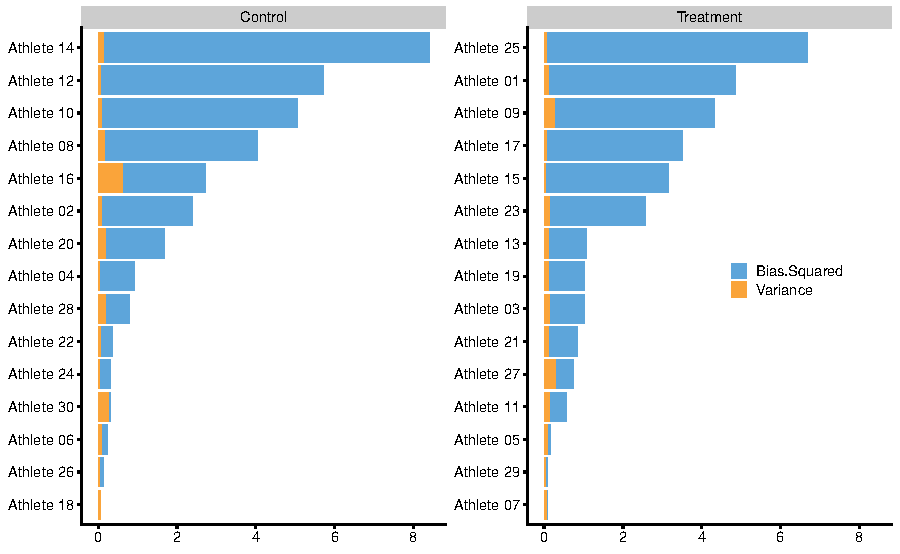
\includegraphics[width=0.9\linewidth]{04-Causal-inference_files/figure-latex/interaction-rct-subj-bias-var-1} 

}

\caption{\textbf{Bias-variance across 10 times repeated 3-fold cross-validation for each athlete. } This analysis can also be utilize to flag certain observations (i.e.~athlete in this case) that are troublesome for the predictive model}\label{fig:interaction-rct-subj-bias-var}
\end{figure}



Interpreting and understanding \emph{direct} and \emph{indirect} effects can be quite difficult, especially when causal structure becomes complex. Visualization techniques such as already mentioned PDP and ICE graphs can be utilized to understand the causal mechanism (Zhao and Hastie \protect\hyperlink{ref-zhaoCausalInterpretationsBlackBox2019}{2019}; Goldstein et al. \protect\hyperlink{ref-goldsteinPeekingBlackBox2013}{2013}). These techniques can also be implemented in observational studies, but with considerable domain knowledge and assumptions needed (Zhao and Hastie \protect\hyperlink{ref-zhaoCausalInterpretationsBlackBox2019}{2019}). Although predictive analysis, particularly those using \emph{black box} machine learning models, has been criticized to lack causal interpretation (Hernán, Hsu, and Healy \protect\hyperlink{ref-hernanSecondChanceGet2019}{2019}; Pearl and Mackenzie \protect\hyperlink{ref-pearlBookWhyNew2018}{2018}; Pearl \protect\hyperlink{ref-pearlSevenToolsCausal2019}{2019}), they can complement causal (or explanatory) analysis (Breiman \protect\hyperlink{ref-breimanStatisticalModelingTwo2001}{2001}; Shmueli \protect\hyperlink{ref-shmueliExplainPredict2010}{2010}; Yarkoni and Westfall \protect\hyperlink{ref-yarkoniChoosingPredictionExplanation2017}{2017}). Figure \ref{fig:pdp-ice-interaction-rct} depicts PDP and ICE plots for Group and Strength 1RM predictors.

\begin{figure}[!htb]

{\centering 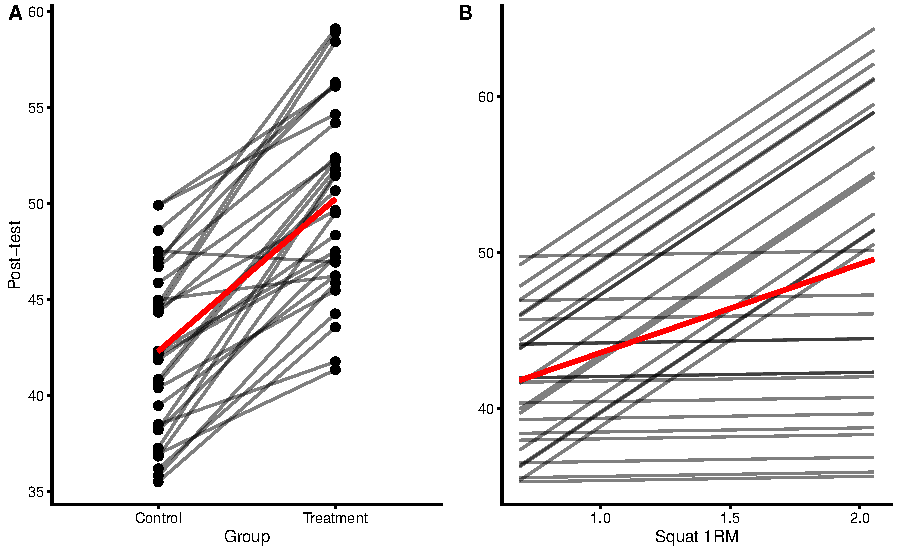
\includegraphics[width=0.9\linewidth]{04-Causal-inference_files/figure-latex/pdp-ice-interaction-rct-1} 

}

\caption{\textbf{PDP and ICE plots for Group and Strength 1RM predictors using RCT model with interaction}}\label{fig:pdp-ice-interaction-rct}
\end{figure}



Since this is RCT, we can give causal interpretation to PDP and ICE plot, particularly panel B in the Figure \ref{fig:pdp-ice-interaction-rct}. According to this analysis (given the data and the model), if one increase Squat 1RM, the effect of treatment (i.e.~plyometric training) will be higher. This can be further analyzed using each athlete. The question we would like to answer (given the data collected and the model) is ``How would particular athlete respond to the treatment if his strength was higher or lower?''. Figure \ref{fig:individual-ice} shows ICE plots in separate facets. This gives us the ability to analyze (given the data and the model) how would each athlete respond if his or her Squat 1RM changed.

\begin{figure}[!htb]

{\centering \includegraphics[width=0.9\linewidth]{04-Causal-inference_files/figure-latex/individual-ice-1} 

}

\caption{\textbf{ICE plots for each athlete}}\label{fig:individual-ice}
\end{figure}



Figure \ref{fig:interaction-rct-counterfactual-effects} depicts predicted ITE (i.e.~what would happen if Groups \emph{flipped} and everything else being equal). If we compare Figure \ref{fig:interaction-rct-counterfactual-effects} with Figure \ref{fig:ancova-rct-counterfactual-effects}, we can quickly see that the ITEs differ and are not equal for every individual. If we calculate the \texttt{mean} of the ITEs (i.e.~arrow lengths), we will get an estimate of \texttt{ATE}. \texttt{SD} of ITEs will give us estimate how variable the treatment effects are, or estimate of \texttt{VTE}. Since these are predicted with the model, I've used the terms \texttt{pATE} and \texttt{pVTE} indicating that they are estimated with the predictive model.

\begin{figure}[!htb]

{\centering \includegraphics[width=0.9\linewidth]{04-Causal-inference_files/figure-latex/interaction-rct-counterfactual-effects-1} 

}

\caption{\textbf{Individual counterfactual prediction when the Group changes.} This way we can estimate model counterfactual predictions when the treatment changes (i.e.~Controls receive treatment, and Treatment doesn't receive treatment). Arrows thus represent model predicted \emph{Individual Treatment Effects} (ITE). Vertical line indicates observed Change}\label{fig:interaction-rct-counterfactual-effects}
\end{figure}



Table \ref{tab:rct-models-performance-comparison} contains comparison between the ANCOVA RCT model (\(\widehat{Post} = \hat{\beta_0} + \hat{\beta_1}Group + \hat{\beta_2}Pre\)) and model with Squat 1RM and interaction term (\(\widehat{Post} = \hat{\beta_0} + \hat{\beta_1}Group + \hat{\beta_2}Pre + \hat{\beta_3}Squat\:1RM + \hat{\beta_4}Group:Squat\:1RM\)) for few estimators that are insightful for the comparison.



\begin{table}

\caption{\label{tab:rct-models-performance-comparison}\textbf{Comparison between two models using few estimators and performance metrics}}
\centering
\begin{tabular}[t]{lrr}
\toprule
estimator & ANCOVA.model & Interaction.model\\
\midrule
Training RMSE & 3.31 & 1.08\\
Training PPER & 0.54 & 0.97\\
Training SESOI to RMSE & 1.51 & 4.64\\
Training R-squared & 0.75 & 0.97\\
CV RMSE & 3.68 & 1.46\\
\addlinespace
CV PPER & 0.50 & 0.91\\
CV SESOI to RMSE & 1.36 & 3.43\\
CV R-squared & 0.69 & 0.95\\
SD Residual (Treatment) & 1.43 & 1.12\\
SD Residual (Control) & 4.64 & 1.11\\
\addlinespace
pATE (Treatment) & -7.85 & -7.57\\
pATE (Control) & 7.85 & 8.33\\
pVTE (Treatment) & 0.00 & 4.62\\
pVTE (Control) & 0.00 & 2.84\\
\bottomrule
\end{tabular}
\end{table}

As can be seen in the Table \ref{tab:rct-models-performance-comparison}, linear model with interactions predicts Post-test in the vertical jump height better than the ANCOVA model. This means that the variance in the treatment effect (\texttt{SD\ Residual} in the Table \ref{tab:rct-models-performance-comparison}) is now explained with additional variables and their interactions\footnote{If you remember the footnote discussion on aleatory and epistemic uncertainty, this is example where what we believed to be aleatory uncertainty (inter-individual residual error or variation that we could not predict: \texttt{SD\ Residual} in the Table \ref{tab:rct-models-performance-comparison}) was actually epistemic uncertainty that we reduced with introducing new variables (Squat 1RM and interaction term) to the model. Although the inter-individual variation in the treatment effect remains (\(SD_{TE}\) or \(SD_{IR}\)), we are now able to predict individual responses more accurately.}.

We are not only interested in prediction, but rather in the underlying causal structure and explaining this model performance when we \emph{intervene} on variables (i.e.~what happens to the target variable when I change X from \emph{a} to \emph{b}, while keeping other variables fixed - which is \emph{ceteris paribus} condition). For this reason, PDP and ICE plots can be used to give causal interpretation of the model (see Figure \ref{fig:pdp-ice-interaction-rct}).
The main critique of Judea Pearl regarding the use of predictive models and techniques is the lack of counterfactual causal interpretation (Pearl and Mackenzie \protect\hyperlink{ref-pearlBookWhyNew2018}{2018}; Pearl \protect\hyperlink{ref-pearlSevenToolsCausal2019}{2019}), particularly with observational studies. I agree that ``the role of expert knowledge is the key difference between prediction and causal inference tasks'' (Hernán, Hsu, and Healy \protect\hyperlink{ref-hernanSecondChanceGet2019}{2019}, 44) and that ``both prediction and causal inference require expert knowledge to formulate the scientific question, but only causal inference requires causal expert knowledge to answer the question'' (Hernán, Hsu, and Healy \protect\hyperlink{ref-hernanSecondChanceGet2019}{2019}, 45), but this doesn't negate the need for providing predictive performance, as well as helping in interpreting the model when such data is available (Zhao and Hastie \protect\hyperlink{ref-zhaoCausalInterpretationsBlackBox2019}{2019}).

According to Zhao and Hastie (Zhao and Hastie \protect\hyperlink{ref-zhaoCausalInterpretationsBlackBox2019}{2019}, 1): ``There are three requirements to make causal interpretations: a model with good predictive performance, some domain knowledge in the form of a causal diagram and suitable visualization tools.''. The common denominator among multiple experts is that for causal inference and causal interpretation there is a need for domain knowledge, particularly when RCTs are not available. This domain knowledge can be made more transparent by using DAGs and other structural diagrams, and thus help in falsifying assumptions (Gelman and Hennig \protect\hyperlink{ref-gelmanSubjectiveObjectiveStatistics2017}{2017}; Hernán \protect\hyperlink{ref-hernanCausalDiagramsDraw2017}{2017}; Hernan \protect\hyperlink{ref-hernanCausalKnowledgePrerequisite2002}{2002}; Hernán, Hsu, and Healy \protect\hyperlink{ref-hernanSecondChanceGet2019}{2019}). Adding prediction to explanatory models can be seen as complement, particularly since statistical analysis has been neglecting predictive analysis over explanatory analysis (Breiman \protect\hyperlink{ref-breimanStatisticalModelingTwo2001}{2001}; Shmueli \protect\hyperlink{ref-shmueliExplainPredict2010}{2010}; Yarkoni and Westfall \protect\hyperlink{ref-yarkoniChoosingPredictionExplanation2017}{2017}).

\hypertarget{model-selection}{%
\subsection{Model selection}\label{model-selection}}

Besides applying model with a single interaction term, we can also apply models with more interactions, or quadratic or polynomial terms, or what have you. As we have seen in the \protect\hyperlink{prediction}{Prediction} chapter, these models can overfit quite easily. That is why we utilized cross-validation to check for model performance on the unseen data. But what if two or more models of different complexity perform similarly on the unseen data (i.e.~when cross-validated)? This is the problem of \emph{model selection and comparison}. Generally, we want to select the simplest model that gives us reliable predictions. Discussions regarding the model comparison and model selection are beyond the scope of this book, although I will provide few examples in the second part of the book.

The model definition should rely on pre-existing beliefs (i.e.~subject-matter expert knowledge) around causal structure underlying intervention. If the statistical analysis is done to \emph{confirm} the structural causal model, then this represents \emph{confirmatory analysis}. Usually, these studies need to be \emph{pre-registered} with the exact analysis workflow and assumption defined \emph{before} data is collected. This is required because in the \emph{exploratory analysis} one can \emph{play} with the data, different models can be tried and the model that fits the data best can be selected. Exploratory analysis is useful for generating models and hypothesis for future studies, but also introduces \emph{hindsight bias} since the model is selected \emph{after} seeing the data or the results of multiple analyses. Very related is so called \emph{p-harking} (Hypothesizing After Results are Known) which involves modifying the hypothesis or in this case causal model, after seeing the results, most often with the aim to reach \emph{statistical significance} (discussed later in the \protect\hyperlink{statistical-inference}{Statistical inference} section). In predictive analysis this hindsight bias is reduced by using hold-out sample, cross-validation, and evaluating the final model performance on the data that has not been seen by the model.

\hypertarget{ergodicity}{%
\section{Ergodicity}\label{ergodicity}}

\emph{Ergodic} process is underlying DGP that is equivalent at \emph{between-individual} (or inter-individual; or group-based analysis) and \emph{within-individual} (or intra-individual or simply individual-based analysis) levels. Thus the causal effects identified using between-individual analysis can be applied to understand within-individual causation as well. \emph{Non-Ergodic} process on the other hand differs between these two levels and effects identified at between-individual level cannot be inferred to within individual level.

Few authors have already brought into question the generalizability of group-based research to individual-based prediction and causal inferences (Fisher, Medaglia, and Jeronimus \protect\hyperlink{ref-fisherLackGrouptoindividualGeneralizability2018}{2018}; Glazier and Mehdizadeh \protect\hyperlink{ref-glazierChallengingConventionalParadigms2018}{2018}; Molenaar \protect\hyperlink{ref-molenaarManifestoPsychologyIdiographic2004}{2004}; Molenaar and Campbell \protect\hyperlink{ref-molenaarNewPersonSpecificParadigm2009}{2009}). Here is an interesting quote from Molenaar (Molenaar and Campbell \protect\hyperlink{ref-molenaarNewPersonSpecificParadigm2009}{2009}, 112):

\begin{quote}
``Most research methodology in the behavioral sciences employs inter-individual analyses, which provide information about the state of affairs of the population. However, as shown by classical mathematical-statistical theorems (the ergodic theorems), such analyses do not provide information for, and cannot be applied at, the level of the individual, except on rare occasions when the processes of interest meet certain stringent conditions. When psychological processes violate these conditions, the inter-individual analyses that are now standardly applied have to be replaced by analysis of intra-individual variation in order to obtain valid results.''
\end{quote}

The individual counterfactual predictions (ITEs) and ICE plots thus rely on ergodicity, which represents big assumption. This means that we should be cautious when generalizing model predictions and causal explanations from group-based level to individual-level.

Data analysis at the individual level (i.e.~collecting multiple data point for individuals) and identifying individual causal effects and predictions might be the step forward, but even with such an approach we are \emph{retrodicting} under \emph{ceteris paribus} conditions and we might not be able to predict future responses. For example, if we have collected responses to various interventions for a particular individual, we might not be able to estimate with certainty how he or she is going to respond to a familiar treatment in the future, since such a prediction relies on \emph{stationarity} of the parameters or the underlying DGP (Molenaar and Campbell \protect\hyperlink{ref-molenaarNewPersonSpecificParadigm2009}{2009}).

But this doesn't imply that all our efforts are useless. We just need to accept the uncertainty and the assumptions involved. For example, for completely novel subject, the best response estimate or prediction estimate is the expected response calculated by using the group-based analysis (i.e.~average treatment effect). This represents the most likely response or prediction. But on top of providing these distribution-based or group-based estimates, one can provide expected uncertainties showing individual-based or response proportions as anchor-based (magnitude-based) estimates (Estrada, Ferrer, and Pardo \protect\hyperlink{ref-estradaStatisticsEvaluatingPrepost2019}{2019}; Norman et al. \protect\hyperlink{ref-normanRelationDistributionAnchorBased2001}{2001}). It is important to note that these usually estimate the same information (Estrada, Ferrer, and Pardo \protect\hyperlink{ref-estradaStatisticsEvaluatingPrepost2019}{2019}; Norman et al. \protect\hyperlink{ref-normanRelationDistributionAnchorBased2001}{2001}); e.g.~the higher the \texttt{Cohen\textquotesingle{}s\ d} the higher the proportion of higher responses. Thus reporting magnitude-based proportions as uncertainties together with expected responses using average-based approach at least help in communicating uncertainties much better than reporting solely average-based estimates. When warranted with the research question, researchers should also report predictive performances on unseen data, as well as underlying assumption using graphical models such as DAGs.

It might be the best to conclude the section on causal inference with the quote from Andrew Gelman's paper (Gelman \protect\hyperlink{ref-gelmanCausalityStatisticalLearning2011}{2011}, 965):

\begin{quote}
``Casual inference will always be a challenge, partly because our psychological intuitions do not always match how the world works. We like to think of simple causal stories, but in the social world, causes and effects are complex. We---in the scientific community---still have not come to any agreement on how best to form consensus on causal questions: there is a general acceptance that experimentation is a gold standard, but it is not at clear how much experimentation should be done, to what extent we can trust inference from observational data, and to what extent experimentation should be more fully incorporated into daily practice (as suggested by some in the ``evidence-based medicine'' movement)."
\end{quote}

\hypertarget{statistical-inference}{%
\chapter{Statistical inference}\label{statistical-inference}}

Why did estimates diverge from the \emph{true} parameters in the previous examples? Why did estimated treatment effect differed from the true treatment effect we used to generate the data? This brings us to the important concept in statistical analysis: a difference between the \emph{true parameter} in the \emph{population} and the \emph{sample estimate}. Population refers to all members of specified group, whereas sample contains only a part, or a subset of a population from which it is taken. To generate the data in simulations, we have assumed DGP in the population, out of which a single or multiples samples were drawn.

The mathematical notation to differentiate true population parameters and sample estimates, or statistics involve using Greek letters to represent true population parameters, and Latin letters to represent sample estimates. For example, \(\mu\) stands for true \texttt{population\ mean}, while \(\bar{x}\) stand for \texttt{sample\ mean}, where \emph{bar} symbol (" \(\bar{}\) ``) indicates \emph{mean}. When it comes to standard deviation, \(\sigma\) stands for true population parameter, while \texttt{SD} stands for sample estimate. Sometimes the \emph{hat} symbol ('' \(\hat{}\) ") is used to denote estimator. For example, \(\hat{y_i}\) would be a model estimate or prediction of the observed \(y_i\).

The difference between the true population parameter and the sample estimate (assuming correctly identified and represented DGP among other issues such as the use of non-biased estimators for example) is due to the \emph{sampling error}, that we will covered shortly. In the simulations, we are certain about the true population parameters, but in \emph{real life} we are \emph{uncertain} about the true parameters and we need to somehow quantify this uncertainty. This is the objective of statistical inference. In other words, with statistical inference we want to generalize from sample to a population, while taking into account uncertainties of the estimates.

\hypertarget{two-kinds-of-uncertainty-two-kinds-of-probability-two-kinds-of-statistical-inference}{%
\section{Two kinds of uncertainty, two kinds of probability, two kinds of statistical inference}\label{two-kinds-of-uncertainty-two-kinds-of-probability-two-kinds-of-statistical-inference}}

In the previous RCT example, by using the Pre-Test score and Group variables, we have estimated predictive performance of the model using Post-test as the target variable. Error (or uncertainty) around individual Post-test score was much bigger than SESOI, which made individual prediction practically useless. This prediction uncertainty decreased as new variables were introduced to the prediction model. With model involving Squat 1RM variable, we have achieved much better predictive performance. This type of uncertainty can be called \emph{epistemic uncertainty} (O'Hagan \protect\hyperlink{ref-ohaganDicingUnknown2004}{2004}), which is a result of lack of knowledge or incomplete information.

In the \protect\hyperlink{prediction}{Prediction} section of this book, I have utilized \emph{irreducible error} in the DGP to represent stochastic component or the random error. Due to this random error, scores will differ from sample to sample. This type of uncertainty can be called \emph{aleatory uncertainty} (O'Hagan \protect\hyperlink{ref-ohaganDicingUnknown2004}{2004}), which results due intrinsic randomness. Another flagship example of the aleatory uncertainty is tossing a dice, drawing a card from a shuffled pack, or random sampling that produces the sampling error.

You can argue of course that aleatory uncertainty is ultimately epistemic uncertainty. For example, if I knew infinite details about the dice tossing, I would be able to predict exactly the number that will be landed. Philosophers have been arguing about these issues for ages, and it is not in the domain of this book to delve deeper into the matters of uncertainty.

The theory of statistical inference and statistics in general rests on describing uncertainties by using \emph{probability}. Since there are two kinds of uncertainty, there are two kinds of probabilities and their meaning. Aleatory uncertainties, like tossing a dice or random sampling, are described using \emph{long-frequency} definition of probability. For example, it can happen that I toss six for 4 times in a row, but in the long-run, which means infinite number of times, probability of tossing a six is equal to 1/6, or probability of 0.166, or 16.6\% (assuming a fair dice of course). Probability viewed from this perspective represents long-frequency number of occurrences of the event of interest, divided by number of total events. For example, if I toss a dice for 1000 times, and if I get number six for 170 times, the probability of tossing a six is equal to 170 / 1000, or 17\%.

With epistemic uncertainty, probability of a proposition simply represents a \emph{degree-of-belief} in the truth of that proposition (O'Hagan \protect\hyperlink{ref-ohaganDicingUnknown2004}{2004}). The degree-of-belief interpretation of probability is referred to as \emph{subjective probability} or \emph{personal probability}, while long-frequency interpretation of probability is referred to as \emph{objective probability}. There are two major schools of statistical inference leaning either on long-frequency interpretation of probability, called \emph{frequentist}, or leaning on degree-of-belief interpretation of probability, called \emph{Bayesian}. There are of course many nuances and other schools of statistical inference (Dienes \protect\hyperlink{ref-dienesUnderstandingPsychologyScience2008}{2008}; Efron and Hastie \protect\hyperlink{ref-efronComputerAgeStatistical2016}{2016}; Gelman and Hennig \protect\hyperlink{ref-gelmanSubjectiveObjectiveStatistics2017}{2017}) which are beyond the scope of this book. The additional approach to inference that will be considered in this book as a preferred approach is the \emph{bootstrap} (Efron and Hastie \protect\hyperlink{ref-efronComputerAgeStatistical2016}{2016}; Hesterberg \protect\hyperlink{ref-hesterbergWhatTeachersShould2015}{2015}; Guillaume A Rousselet, Pernet, and Wilcox \protect\hyperlink{ref-rousseletPercentileBootstrapTeaser2019}{2019}\protect\hyperlink{ref-rousseletPercentileBootstrapTeaser2019}{b}, \protect\hyperlink{ref-rousseletPracticalIntroductionBootstrap2019}{2019}\protect\hyperlink{ref-rousseletPracticalIntroductionBootstrap2019}{a}). But more about it later.

To better explain the differences between the frequentist and Bayesian approach to statistical inference I am going to use known male mean height and SD in the population. The population parameter of interest is the \texttt{population\ mean} (Greek \(\mu\)) estimated using the \texttt{sample\ mean} (\(\bar{x}\)).

\hypertarget{frequentist-perspective}{%
\chapter{Frequentist perspective}\label{frequentist-perspective}}

As already stated, using simulations is outstanding teaching tool (Carsey and Harden \protect\hyperlink{ref-carseyMonteCarloSimulation2013}{2013}; Hopkins \protect\hyperlink{ref-hopkinsUnderstandingStatisticsUsing2007}{2007}), and also very useful for understanding the frequentist inference as well. Figure \ref{fig:sampling-distribution-of-the-mean} (Panels A and B) depicts hypothetical male population where mean height \(\mu\) is 177.8cm and SD (\(\sigma\)) is 10.16cm. From this population we are randomly \emph{drawing} N=5 (left side panels on Figure \ref{fig:sampling-distribution-of-the-mean}) and N=20 (right side panels on Figure \ref{fig:sampling-distribution-of-the-mean}) individuals for which we estimate the \texttt{mean} height. Individuals are represented as blue dots (Panels C and D on Figure \ref{fig:sampling-distribution-of-the-mean}), whereas estimated \texttt{mean} height is depicted as orange dot. Now imagine we repeat this sampling 50 times, calculate the mean for every sample, and then draw the distribution of the sampled means (Panels E an F on Figure \ref{fig:sampling-distribution-of-the-mean}). This distribution is called \emph{sampling distribution of the \texttt{sample\ mean}} and the \texttt{SD} of this distribution is referred to as \emph{standard error} or \emph{sampling error}. Since our estimate of interest is the \texttt{mean}, standard deviation of the sampling distribution of the mean is called \emph{standard error of the mean} (\texttt{SEM}). On Panels E and F in the Figure \ref{fig:sampling-distribution-of-the-mean}, mean of the sampling \texttt{means} is indicated by a black dot, and error bars represent \texttt{SEM}.

\begin{figure}[!htb]

{\centering \includegraphics[width=0.9\linewidth]{06-Frequentist-perspective_files/figure-latex/sampling-distribution-of-the-mean-1} 

}

\caption{\textbf{Sampling distribution of the \texttt{mean}. A and B. }Distribution of the height in the population. From this population we draw samples. \textbf{C and D.} 50 sample are taken with N=5 (panel C) and N=20 (panel D) observations. Each observation is indicated by a blue dot. Calculated \texttt{mean}, as a parameter of interest, is indicated by an orange dot. \textbf{E and F.} Distribution of collected sample \texttt{means} from panels C and D. This distribution of the sample \texttt{means} is narrower, indicating higher precision when higher N is used. Black dot indicates the mean of the sample \texttt{means}, with error bars indicating \texttt{SD} of sample means. Orange line represents hypothetical distribution of the sample \texttt{means} when number of samples is infinitely large}\label{fig:sampling-distribution-of-the-mean}
\end{figure}



As can be seen from the Figure \ref{fig:sampling-distribution-of-the-mean}, the sampling distribution of the \texttt{mean} looks like normal distribution. If the number of samples reach very large number or \emph{infinity}, the sampling distribution of the \texttt{mean} will eventually be distributed with the \texttt{SEM} equal to (Equation \eqref{eq:sem-equation}):

\begin{equation}
  SEM = \frac{\sigma}{\sqrt{N}}
  \label{eq:sem-equation}
\end{equation}

This \emph{theoretical} distribution is overlaid on the acquired sampling distribution from 50 samples in the Figure \ref{fig:sampling-distribution-of-the-mean} (Panels E and F). Since the true \(\sigma\) is not known, sample \texttt{SD} is utilized instead, in order to estimate the true \texttt{SEM} (Equation \eqref{eq:estimated-sem-equation}):

\begin{equation}
  \hat{SEM} = \frac{SD}{\sqrt{N}}
  \label{eq:estimated-sem-equation}
\end{equation}

The take-home point is that the larger the sample, the smaller the standard error, which is visually seen as narrower sampling distribution (compare N=5 and N=20 sampling distributions on Figure \ref{fig:sampling-distribution-of-the-mean}). Another conclusion regarding frequentist inference, is that calculated probabilities revolve around sampling distribution of the sample \texttt{mean} and other long-frequency sampling distributions. Everything else are details. But as the saying goes, the devil is in the details.

Sampling distributions and equations for standard errors are derived algebraically for most estimators (e.g.~\texttt{mean}, \texttt{SD}, \texttt{Cohen\textquotesingle{}s\ d}), but for some estimators it might be hard to derive them, so other solutions do exist (like \emph{bootstrapping} which will be covered in \protect\hyperlink{bootstrap}{Bootstrap} section). For example, sampling distribution of the change score proportions can be very difficult to be derived algebraically (Swinton et al. \protect\hyperlink{ref-swintonStatisticalFrameworkInterpret2018}{2018}). For some estimators, mean of the long-frequency samples is different than the true population value, thus these estimators are termed \emph{biased estimators}. One example of the biased estimator would be \texttt{SD} of the sample where we divide with \(N\), instead of \(N-1\). Estimators that have the mean of the long-frequency sample estimate equal to the true population parameter are called \emph{unbiased estimators}.

Although the sampling distribution of the \texttt{mean} looks like a normal distribution, it actually belongs to the \emph{Student's t} distribution, which has fatter tails for smaller samples (Figure \ref{fig:student-distribution}). Besides \texttt{mean} and \texttt{SD}, Student's t distribution also has \emph{degrees of freedom} (DF) parameters, which is equal to N-1 for the sample \texttt{mean}. Normal distribution is equal to Student's t distribution when DF is infinitely large.

\begin{figure}[!htb]

{\centering \includegraphics[width=0.9\linewidth]{06-Frequentist-perspective_files/figure-latex/student-distribution-1} 

}

\caption{\textbf{Student's t-distribution}}\label{fig:student-distribution}
\end{figure}



Since Student's t distribution is fatter on the tails, critical values that cover 90, 95, and 99\% of distribution mass are different than the commonly used ones for the normal distribution. Table \ref{tab:student-critical-values} contains critical values for different DF. For example, 90\% of the sampling distribution will be inside the \(\bar{x} \pm 1.64 \times SEM\) interval for the normal distribution, but for Student t with DF=5, 90\% of the sampling distribution will be inside the \(\bar{x} \pm 2.02 \times SEM\) interval.



\begin{table}

\caption{\label{tab:student-critical-values}\textbf{Critical values for Student's t distribution with different degrees of freedom}}
\centering
\begin{tabular}[t]{lrrrrr}
\toprule
 & 50\% & 90\% & 95\% & 99\% & 99.9\%\\
\midrule
DF=5 & 0.73 & 2.02 & 2.57 & 4.03 & 6.87\\
DF=10 & 0.70 & 1.81 & 2.23 & 3.17 & 4.59\\
DF=20 & 0.69 & 1.72 & 2.09 & 2.85 & 3.85\\
DF=30 & 0.68 & 1.70 & 2.04 & 2.75 & 3.65\\
DF=50 & 0.68 & 1.68 & 2.01 & 2.68 & 3.50\\
\addlinespace
(Normal) & 0.67 & 1.64 & 1.96 & 2.58 & 3.29\\
\bottomrule
\end{tabular}
\end{table}

\hypertarget{null-hypothesis-significance-testing}{%
\section{Null-Hypothesis Significance Testing}\label{null-hypothesis-significance-testing}}

There are two approaches to statistical inference, be it frequentist or Bayesian: \emph{hypothesis testing} and \emph{estimation} (Cumming \protect\hyperlink{ref-cummingNewStatisticsWhy2014}{2014}; Kruschke and Liddell \protect\hyperlink{ref-kruschkeBayesianNewStatistics2018}{2018}\protect\hyperlink{ref-kruschkeBayesianNewStatistics2018}{b}). I will focus on the former, although latter will be covered as well. For the frequentist inference, mathematics behind both of these are the same and both involve standard errors.

\emph{Null-hypothesis significance testing} (NHST) is still one of the most dominant approaches to statistical inference, although heavily criticized (for example see (Cumming \protect\hyperlink{ref-cummingNewStatisticsWhy2014}{2014}; Kruschke and Liddell \protect\hyperlink{ref-kruschkeBayesianNewStatistics2018}{2018}\protect\hyperlink{ref-kruschkeBayesianNewStatistics2018}{b})). In Figure \ref{fig:sampling-distribution-of-the-mean}, we have sampled from the known population, but in practice we don't know the true parameter values in the population, nor we are able to collect data from the whole population (unless it is a small one, but there is no need for statistical inference then, since the whole population is represented in our sample). Thus, we need to use sampled data to make inferences about the population. With NHST we want to \emph{test} sample parameter or estimator (i.e.~\texttt{mean} in this case) against the null-hypothesis (\(H_{0}\)). Null-hypothesis usually takes the \emph{no effect} value, but it can take any value of interest for the researcher.

Although this sounds mouthful, a simple example will make it clearer. Imagine that we do know the true population \texttt{mean} height, but in one particular region the \texttt{mean} height of the sample differs from the known population \texttt{mean}. If we assume that this region belongs to the same population, then we want to test to see how likely are we to sample \texttt{mean} we have acquired or more extreme.

Figure \ref{fig:null-hypothesis} contains known population \texttt{mean} height as the null-hypothesis and estimated probabilities of observing sample \texttt{mean} of 180, 182.5, and 185cm (or +2.2, +4.7, +7.2cm difference) \emph{or larger} for sample sizes N=5, N=10 and N=20. Panel A on Figure \ref{fig:null-hypothesis} depicts \emph{one-sided} approach for estimating probability of observing these sample \texttt{mean} heights. One-sided approach is used when we are certain about the direction of the effect. \emph{Two-sided} approach, on the other hand, calculates probability for the effect of the unknown direction. In this example that would be sample \texttt{mean} height difference of ±2.2, ±4.7, ±7.2cm or larger. Two-sided approach is depicted on the Panel B (Figure \ref{fig:null-hypothesis}).

\begin{figure}[!htb]

{\centering \includegraphics[width=0.9\linewidth]{06-Frequentist-perspective_files/figure-latex/null-hypothesis-1} 

}

\caption{\textbf{Null-hypothesis significance testing. }Assuming null-hypothesis (true parameter value, or parameter value in the population, in this case \texttt{mean} or \(\mu\)) is true, probability of observing sample parameter of a given magnitude or larger, is estimated by calculating proportion of sampling distribution that is over sample parameter value. The larger the sample size, the smaller the width of the sampling distribution. \textbf{A.} One-sided approach is used when we are certain about the direction of the effect. \textbf{B.} Two-sided approach is used when expected direction of the effect is unknown}\label{fig:null-hypothesis}
\end{figure}



The calculated probability of observing sample mean or larger, given null-hypothesis, is called \emph{p-value}. In other words, p-value is the probability of observing data (in this case sample \texttt{mean}) given the null hypothesis (Equation \eqref{eq:p-value-equation})

\begin{equation}
  p \; value = p(Data | H{0}) 
  \label{eq:p-value-equation}
\end{equation}

It is easy to interpret p-values as ``probability of the null hypothesis (given data)'' (\(p(H{0}|Data)\)), but that is erroneous. This is Bayesian interpretation (also called \emph{inverse probability}) which is quite common, even for the experienced researchers. Unfortunately, p-values cannot be interpreted in such way, but rather as a ``probability of data given null hypothesis''.

As you can see from the Figure \ref{fig:null-hypothesis}), for the same difference in sample \texttt{mean} height, different sample sizes will produce different p-values. This is because sampling distribution of the \texttt{mean} will be narrower (i.e.~smaller \texttt{SEM}) as the sample size increase. In other words, for the same effect (in this case sample \texttt{mean}), p-value will be smaller as the sample size gets bigger. It is thus important to realize that p-values don't tell us anything about the magnitude of the effect (in this case the difference between the sample \texttt{mean} and the known population \texttt{mean}).

The procedures of acquiring p-values are called \emph{statistical tests}. With the example above, we are using one variation of the \emph{Student t test}, where we are calculating the test value \emph{t} using the following Equation \eqref{eq:t-test}.

\begin{equation}
  \begin{split}
  t &= \frac{\bar{x} -\mu}{SEM} \\
  \\
  t &= \frac{\bar{x} -\mu}{\frac{SD}{\sqrt{N}}}
  \end{split}
  \label{eq:t-test}
\end{equation}

P-value is then estimated by using the calculated t value and appropriate Student's t distribution (see Figure \ref{fig:student-distribution}) to calculate the surface area over a particular value of t. This is usually done in the statistical program, or by using tables similar to Table \ref{tab:student-critical-values} .

Once the p-value is estimated, we need to decide whether to reject the null-hypothesis or not. In order to do that, we need to define the error we are willing to accept. This error is called \emph{alpha} (Greek \(\alpha\)) or \emph{Type I} error and refers to making an error of rejecting the null-hypothesis when null-hypothesis is true. Out of sheer convenience, alpha is set to 0.1 (10\% error), 0.05 (5\% error) or 0.01 (1\% error).

If p-value is smaller than alpha, we will reject the null-hypothesis and state that the effect has \emph{statistical significance}. The statistical significance has bad wording since it does not imply magnitude of the effect, only that the sample data come from a different population assumed by null-hypothesis.

Take the following example. Let's assume we have sample size of N=20 where sample \texttt{mean} is equal to 185cm. Using the known population \texttt{mean} (177.8cm) and \texttt{SD} (10.16cm), we get that \(t=3.17\). Using two-sided test and alpha=0.05, can we reject the null-hypothesis? In order to do this we can refer to Table \ref{tab:student-critical-values} and check that for DF=20 (which is not exact, but it will serve the purpose), 95\% of sampling distribution (which leaves 2.5\% on each tail which is equal to 5\% alpha) will be within ±2.08. Since calculated \(t=3.17\) is over ±2.08, we can reject the null-hypothesis with alpha=0.05. Figure \ref{fig:null-hypothesis} (Panel B) depicts the exact p-value for this example, which is equal to p=0.005. Statistical software can calculate exact p-values, but before these were available, tables and procedure just describes were used instead.

\hypertarget{statistical-power}{%
\section{Statistical Power}\label{statistical-power}}

There is other type of error that we can commit: \emph{Type II} error or \emph{beta} (Greek \(\beta\)). In order to understand Type II error, we need to assume alternate hypothesis or \(H{a}\). Type II error refers to the error we make when we reject the alternate-hypothesis when alternate-hypothesis is true. Type I and Type II error are inversely related - the more we are willing to make Type I errors, the less likely we are going to make Type II errors, and \emph{vice versa} (Table \ref{tab:error-types}).

\begin{longtable}[]{@{}lll@{}}
\caption{\label{tab:error-types} \textbf{Type I and Type II errors}}\tabularnewline
\toprule
& True \(H_{0}\) & True \(H_{a}\)\tabularnewline
\midrule
\endfirsthead
\toprule
& True \(H_{0}\) & True \(H_{a}\)\tabularnewline
\midrule
\endhead
Rejected \(H_{0}\) & Type I &\tabularnewline
Rejected \(H_{a}\) & & Type II\tabularnewline
\bottomrule
\end{longtable}

It is important to keep in mind that with NHST, we never \emph{accept} any hypothesis, we either reject it or not. For example, we never say ``null-hypothesis is accepted (p=0.23)'', but rather ``null-hypothesis is not rejected (p=0.23)''.

Assuming that alternate-hypothesis is true, probability of rejecting the null-hypothesis is equal to \(1-\beta\). This is called \emph{statistical power} and depends on the magnitude of the effect we are aiming to detect (or not-to-reject to correct myself). Figure \ref{fig:statistical-power} depicts multiple examples of one-sided and two-sided statistical power calculations given the known alpha of 0.05 and null-hypothesis for difference in sample mean height of ±2.5, ±5, and ±7.5cm (+2.5, +5, and +7.5cm for one sided test) for N=5, N=10 and N=20.

\begin{figure}[!htb]

{\centering \includegraphics[width=0.9\linewidth]{06-Frequentist-perspective_files/figure-latex/statistical-power-1} 

}

\caption{\textbf{Statistical power. } Statistical power is probability of detecting an effect of particular magnitude or larger. Visually, statistical power is dark blue surface and represents probability of rejecting the null-hypothesis given that the alternative hypothesis is true. \textbf{A.} One-sided approach. \textbf{B.} Two-sided approach}\label{fig:statistical-power}
\end{figure}



As can be seen from the Figure \ref{fig:statistical-power}, the higher the magnitude of the effect (in this case difference in height \texttt{means}), the more likely we are to detect it (by rejecting null-hypothesis). Statistical power is mostly used when planning the studies to estimate sample size needed to detect effects of magnitude of interest (usually using known or observed effect from previous studies, or even SESOI). For example, question such as ``How big of a sample do I need to detect 2.5cm difference with 80\% power, alpha 0.05 and expected sample SD of 10cm?'' is answered by using statistical power analysis. Statistical power, or sample size for needed statistical power can be easily calculated for simple analysis, but for some more elaborate analyses simulations are needed.

The frequentist approach to statistical inference is all about maintaining accepted error rates, particularly Type I, for both tests and estimates. This can be particularly difficult when \emph{family-wise error rates} need to be controlled, and these can emerge when multiple NHST are done. Some techniques, called p-harking, can also introduce bias in the error rates by \emph{fishing} for p-values (e.g.~collecting samples until significant results are found). These topics are beyond the scope of this paper, but one of the reasons why some researchers prefer \protect\hyperlink{bayesian-perspective}{Bayesian perspective}.

\hypertarget{new-statistics-confidence-intervals-and-estimation}{%
\section{New Statistics: Confidence Intervals and Estimation}\label{new-statistics-confidence-intervals-and-estimation}}

Rather than performing NHST, uncertainty of the estimated parameter can be represented with the \emph{confidence interval} (CI). CIs are usually pretty hard to explain and non-intuitive since they do not carry any distributional information.\footnote{It is quite common to erroneously interpret CIs as Bayesian \emph{credible intervals} (Kruschke and Liddell \protect\hyperlink{ref-kruschkeBayesianNewStatistics2018}{2018}\protect\hyperlink{ref-kruschkeBayesianNewStatistics2018}{b}; McElreath \protect\hyperlink{ref-mcelreathStatisticalRethinkingBayesian2015}{2015}).} It is thus better to refer to CIs as \emph{compatibility intervals} (Gelman and Greenland \protect\hyperlink{ref-gelmanAreConfidenceIntervals2019}{2019}), since, let's say 95\% confidence interval contains all the hypotheses parameter values that would not be rejected by p\textless0.05 NHST (Kruschke and Liddell \protect\hyperlink{ref-kruschkeBayesianNewStatistics2018}{2018}\protect\hyperlink{ref-kruschkeBayesianNewStatistics2018}{b}). This implies that, in the long-run (when sampling is repeated infinite number of times), 95\% confidence interval will capture true parameter value 95\% of the time.

Assuming N=20 samples come from the population where the true \texttt{mean} height is equal to 177.8cm and \texttt{SD} is equal to 10.16cm, calculated 95\% CIs around sample parameter estimate (in this case sample \texttt{mean}), in the long run, will capture true population parameter 95\% of the time. Figure \ref{fig:confidence-intervals} depicts first 100 samples out of total of 1,000 taken from the population with calculated 95\% CIs. CIs that missed the true population parameter value are depicted in red. Table \ref{tab:confidence-intervals-summary} contain the summary for this simulation. If this simulation is repeated for many more times, CIs will capture true population parameter 95\% of the time, or in other words, have Type I error of 5\%.

\begin{figure}[!htb]

{\centering \includegraphics[width=0.9\linewidth]{06-Frequentist-perspective_files/figure-latex/confidence-intervals-1} 

}

\caption{\textbf{\(95\%\) confidence intervals for the sample \texttt{mean}, estimated for 100 samples (N=20 observations) drawn from population of known parameters (population \texttt{mean} is indicated by vertical line). }In the long-run, \(95\%\) confidence intervals will span the true population value \(95\%\) of the time. Confidence intervals that didn't span the true population parameter value are colored in red}\label{fig:confidence-intervals}
\end{figure}



\begin{table}

\caption{\label{tab:confidence-intervals-summary}\textbf{Type I errors in 1000 samples}}
\centering
\begin{tabular}[t]{rrr}
\toprule
Sample & Correct \% & Type I Errors \%\\
\midrule
1000 & 95.9 & 4.1\\
\bottomrule
\end{tabular}
\end{table}



Similarly to different alphas, CIs can use different levels of confidence, usually 90\%, 95\%, 99\%. As already mentioned, mathematics behind the confidence intervals is equal to mathematics behind NHST. In order to calculate two-sided CIs for the sample mean, the Equation \eqref{eq:ci-equation} is used:

\begin{equation}
  CI = \bar{x} \pm t_{crit} \times \widehat{SEM} 
  \label{eq:ci-equation}
\end{equation}

\(T_{crit}\) can be found in the Table \ref{tab:student-critical-values}, where for 95\% two-sided confidence and DF=20, is equal to 2.086. Using the example of observed sample mean of 185cm, known sample \texttt{SD} (10.16cm) and N=20 (which is equal to DF=19, but for the sake of example DF=20 will be used), calculated 95\% confidence interval is equal to 180.26 to 189.74cm. From the compatibility interpretation standpoint, this CI means that the hypotheses with values ranging from 180.26 to 189.74cm, will not be rejected with alpha=0.05.

Confidence intervals are great solution for visualizing uncertainties around estimates. Figure \ref{fig:sample-mean-cis} depicts already used example in Figure \ref{fig:null-hypothesis} (two-sided and one-sided p-values), but this time 95\% CIs around the sample \texttt{means} are depicted. Please note that in scenarios where 95\% CIs cross the null-hypothesis, NHST will yield p\textgreater0.05. This means that null-hypothesis is not rejected and results are not statistically significant. CIs can be thus used to visually inspect and conclude whether or not the null-hypothesis would be rejected or not if NHST is performed.

\begin{figure}[!htb]

{\centering \includegraphics[width=0.9\linewidth]{06-Frequentist-perspective_files/figure-latex/sample-mean-cis-1} 

}

\caption{\textbf{\(95\%\) Confidence intervals for sample mean.} Null-hypothesis of the population parameter value is indicated by vertical dashed line. If the \(95\%\) confidence interval doesn't touch or cross the null-hypothesis parameter value, p-value is less than 0.05 and effect is statistically significant (given alpha of 0.05). \textbf{A.} One-sided confidence intervals. \textbf{B.} Two-sided confidence intervals}\label{fig:sample-mean-cis}
\end{figure}



\hypertarget{minimum-effect-tests}{%
\section{Minimum Effect Tests}\label{minimum-effect-tests}}

NHST doesn't tell us anything about the magnitudes of the effect. Just because the test is statistically significant (p\textless0.05), it's doesn't imply practically meaningful effect. Rather than using null-hypothesis of \emph{no effect}, we can perform numerous one-sided NHSTs by using SESOI thresholds to infer practical significance. These are called \emph{minimum effect tests} (METs) and can distinguish between 6 different conclusions: \emph{lower}, \emph{not-higher}, \emph{equivalent}, \emph{not-lower}, \emph{higher}, and \emph{equivocal} effect. Figure \ref{fig:effect-magnitudes} depicts how SESOI and CIs can be used to distinguish between these 6 magnitude-based conclusions (Barker and R. Schofield \protect\hyperlink{ref-barkerInferenceMagnitudesEffects2008}{2008}; Sainani et al. \protect\hyperlink{ref-sainaniMagnitudeBasedInference2019}{2019}).

\begin{figure}[!htb]

{\centering \includegraphics[width=0.9\linewidth]{06-Frequentist-perspective_files/figure-latex/effect-magnitudes-1} 

}

\caption{\textbf{Inference about magnitudes of effects.} Error bars represent confidence intervals around estimate of interest. Adapted and modified from Barker and R. Schofield (\protect\hyperlink{ref-barkerInferenceMagnitudesEffects2008}{2008}); Sainani et al. (\protect\hyperlink{ref-sainaniMagnitudeBasedInference2019}{2019})}\label{fig:effect-magnitudes}
\end{figure}



\hypertarget{individual-vs.-parameter-sesoi}{%
\subsection{Individual vs.~Parameter SESOI}\label{individual-vs.-parameter-sesoi}}

So far we have used SESOI to infer practically significant differences or changes at the \emph{individual} level. For example, answering what is the practically meaningful difference in height, SESOI was used to calculate proportions and chances of observing individuals with lower, equivalent and higher magnitudes of effects.

In prediction tasks, SESOI was used to infer practically meaningful prediction error. This helped answering the question regarding whether the individual predictions are within practically equivalent region.

However, apart from using SESOI to infer individual change, difference, and prediction magnitudes, SESOI can also be used to evaluate statistics or parameters against practically significant anchor. For example, in Equation \eqref{eq:diff-to-SESOI}, we have divided \texttt{mean} group difference with SESOI to create magnitude-based estimator. But here, we assumed that the same magnitude used at the individual level is of equal practical importance at the group level (i.e.~aggregate level using the \texttt{mean} estimator). For example, individual change of ±5kg might be practically important at the level of the individual, but not at the level of the group (i.e.~parameter), and \emph{vice versa}. Usually, they are assumed to be the same (see also \protect\hyperlink{ergodicity}{Ergodicity} section).

Since sample \texttt{mean} difference is the estimator of the parameter in the population we are interested in estimating, we tend to use SESOI to give practical anchors for parameters as well. It could be argued that different terms should be used for the parameter SESOI (particularly for standardized estimators such as \texttt{Cohen\textquotesingle{}s\ d}) \emph{versus} individual SESOI. For example, we can use ROPE term for parameters (Kruschke and Liddell \protect\hyperlink{ref-kruschkeBayesianDataAnalysis2018}{2018}\protect\hyperlink{ref-kruschkeBayesianDataAnalysis2018}{a}, \protect\hyperlink{ref-kruschkeBayesianNewStatistics2018}{2018}\protect\hyperlink{ref-kruschkeBayesianNewStatistics2018}{b}), and SESOI for individual-level magnitude inferences. For practical purposes they are considered equal, although I believe further discussion about this distinction is warranted, but outside the scope of this book.

\hypertarget{two-one-sided-tests-of-equivalence}{%
\subsection{Two one-sided tests of equivalence}\label{two-one-sided-tests-of-equivalence}}

Besides testing again null-hypothesis of no-effect, we can use the two one-sided tests (TOST) procedure to test for \emph{equivalence} and reject the presence of the smallest effect size of interest (SESOI) (Lakens, Scheel, and Isager \protect\hyperlink{ref-lakensEquivalenceTestingPsychological2018}{2018}; Lakens \protect\hyperlink{ref-lakensEquivalenceTestsPractical2017}{2017}). TOST involves using two one-sided NHSTs assuming parameter values at SESOI thresholds (Figure \ref{fig:tost}). Since the TOST produces two p-values, the larger of the two is reported. A conclusion of statistical equivalence is warranted when the larger of the two p-values is smaller than alpha (Lakens \protect\hyperlink{ref-lakensEquivalenceTestsPractical2017}{2017}).

From estimation perspective, statistical equivalence at the level of alpha=0.05 can be inferred if the 90\% (90\% not 95\%; it is not a typo) CI falls completely within SESOI band.

\begin{figure}[!htb]

{\centering \includegraphics[width=0.9\linewidth]{06-Frequentist-perspective_files/figure-latex/tost-1} 

}

\caption{\textbf{Equivalence test using two one-sided tests (TOST). }Equivalence test involves two NHSTs at SESOI thresholds and calculates two one-sided p-values, out of which a larger one is reported as result. Error bars represent 90\% confidence intervals.}\label{fig:tost}
\end{figure}



\hypertarget{superiority-and-non-inferiority}{%
\subsection{Superiority and Non-Inferiority}\label{superiority-and-non-inferiority}}

Two same NHSTs at SESOI thresholds are utilized to test superiority and non-inferiority of the effects. In other words, we want to conclude whether the effect is higher and/or not-lower than SESOI. To achieve this, two one-sided NHSTs are performed to estimate the probability of observing effect in the positive direction (Figure \ref{fig:superiority-non-inferiority}).

\begin{figure}[!htb]

{\centering \includegraphics[width=0.9\linewidth]{06-Frequentist-perspective_files/figure-latex/superiority-non-inferiority-1} 

}

\caption{\textbf{Superiority and Non-Inferiority tests. }Similar to equivalence test using TOST procedure, superiority and non-inferiority tests involve two one-sided NHSTs at SESOI thresholds in the positive direction. Error bars represent 90\% confidence intervals.}\label{fig:superiority-non-inferiority}
\end{figure}



\hypertarget{inferiority-and-non-superiority}{%
\subsection{Inferiority and Non-Superiority}\label{inferiority-and-non-superiority}}

To test the inferiority and non-superiority of the effects, two one-sided NHSTs are performed to estimate the probability of observing effect in the negative direction (Figure \ref{fig:inferiority-non-superiority}).

\begin{figure}[!htb]

{\centering \includegraphics[width=0.9\linewidth]{06-Frequentist-perspective_files/figure-latex/inferiority-non-superiority-1} 

}

\caption{\textbf{Inferiority and Non-Superiority tests. }Similar to equivalence test using TOST procedure, inferiority and non-superiority tests involve two one-sided NHSTs at SESOI thresholds in the negative direction. Error bars represent 90\% confidence intervals.}\label{fig:inferiority-non-superiority}
\end{figure}



\hypertarget{inference-from-mets}{%
\subsection{Inference from METs}\label{inference-from-mets}}

The aforementioned METs provide five p-values: for lower (inferiority), not-higher (non-superiority), equivalent (equivalence), not-lower (non-inferiority), and higher (superiority) effect magnitude. These p-values can be used to make magnitude-based inferences about the effects. Figure \ref{fig:met-results} depicts already used examples to calculate p-values from METs and the final inference on the magnitude of the effect (see Figure \ref{fig:effect-magnitudes}).

\begin{figure}[!htb]

{\centering \includegraphics[width=0.9\linewidth]{06-Frequentist-perspective_files/figure-latex/met-results-1} 

}

\caption{\textbf{Minimum Effect Test results. }Error bars represent 90\% confidence intervals.}\label{fig:met-results}
\end{figure}



\hypertarget{magnitude-based-inference}{%
\section{Magnitude Based Inference}\label{magnitude-based-inference}}

Batterham and Hopkins (Batterham and Hopkins \protect\hyperlink{ref-batterhamMakingMeaningfulInferences2006}{2006}; Hopkins et al. \protect\hyperlink{ref-hopkinsProgressiveStatisticsStudies2009}{2009}) proposed novel approach in making meaningful inference about magnitudes, called \emph{magnitude based inference} (MBI). MBI has been recently criticized (Barker and R. Schofield \protect\hyperlink{ref-barkerInferenceMagnitudesEffects2008}{2008}; Borg et al. \protect\hyperlink{ref-borgBayesianMethodsMight2018}{2018}; Curran-Everett \protect\hyperlink{ref-curran-everettMagnitudebasedInferenceGood2018}{2018}; Hopkins and Batterham \protect\hyperlink{ref-hopkinsVindicationMagnitudeBasedInference2018}{2018}; Nevill et al. \protect\hyperlink{ref-nevillCanWeTrust2018}{2018}; Sainani et al. \protect\hyperlink{ref-sainaniMagnitudeBasedInference2019}{2019}; Sainani \protect\hyperlink{ref-sainaniProblemMagnitudebasedInference2018}{2018}; Welsh and Knight \protect\hyperlink{ref-welshMagnitudebasedInferenceStatistical2015}{2015}) for interpreting CIs as Bayesian credible intervals and for not controlling Type I and Type II errors.

As explained, CIs doesn't contain any probability distribution information about the true parameter. Although CIs, Bayesian \emph{credible intervals} (with flat or non-informative \emph{prior}), and \emph{bootstrap CIs} tend to converge to the approximately same values for very simple tests (such as t-test for the sample \texttt{mean}), interpreting CIs established using frequentist approach as Bayesian credible intervals is not valid approach to statistical inference (Sainani et al. \protect\hyperlink{ref-sainaniMagnitudeBasedInference2019}{2019}). Figure \ref{fig:mbi} depicts Bayesian interpretation of the confidence intervals used in MBI.

Using MBI as a simple descriptive approach to interpret CIs can be rationalized, but making inferences from estimated probabilities is not recommended (Caldwell and Cheuvront \protect\hyperlink{ref-caldwellBasicStatisticalConsiderations2019}{2019}). If frequentist approaches are used for magnitude-based statistical inference, METs should be used instead.

\begin{figure}[!htb]

{\centering \includegraphics[width=0.9\linewidth]{06-Frequentist-perspective_files/figure-latex/mbi-1} 

}

\caption{\textbf{Magnitude-based inference use inappropriate Bayesian interpretation of the confidence intervals to calculate lower, equivalent, and higher probabilities of the effect. }Vertical dashed lines represent SESOI. thresholds. Error bars represent 90\% confidence intervals.}\label{fig:mbi}
\end{figure}



There are numerous problems with frequentist inference (Kruschke and Liddell \protect\hyperlink{ref-kruschkeBayesianNewStatistics2018}{2018}\protect\hyperlink{ref-kruschkeBayesianNewStatistics2018}{b}, \protect\hyperlink{ref-kruschkeBayesianDataAnalysis2018}{2018}\protect\hyperlink{ref-kruschkeBayesianDataAnalysis2018}{a}). The results are not intuitive and are usually erroneously interpreted from the Bayesian perspective. Error rates need to be controlled for and adjusted when multiple comparisons are made, or when different \emph{stopping} techniques are used, sampling distributions are unknown for some estimators and cannot be derived algebraically. Various assumptions such as assumptions of normality, non-colinearity and others, need to be made and tested for, and for more complex models, such as \emph{hierarchical models}, p-values and CIs are only approximated (Kruschke and Liddell \protect\hyperlink{ref-kruschkeBayesianDataAnalysis2018}{2018}\protect\hyperlink{ref-kruschkeBayesianDataAnalysis2018}{a}, \protect\hyperlink{ref-kruschkeBayesianNewStatistics2018}{2018}\protect\hyperlink{ref-kruschkeBayesianNewStatistics2018}{b}). It is beyond this short chapter to delve into more details, regarding the frequentist approach to statistical inference, and readers are directed to references provided in this section.

\hypertarget{bayesian-perspective}{%
\chapter{Bayesian perspective}\label{bayesian-perspective}}

Bayesian inference is reallocation of plausibility (credibility) across possibilities (Kruschke and Liddell \protect\hyperlink{ref-kruschkeBayesianDataAnalysis2018}{2018}\protect\hyperlink{ref-kruschkeBayesianDataAnalysis2018}{a}, \protect\hyperlink{ref-kruschkeBayesianNewStatistics2018}{2018}\protect\hyperlink{ref-kruschkeBayesianNewStatistics2018}{b}; McElreath \protect\hyperlink{ref-mcelreathStatisticalRethinkingBayesian2015}{2015}). Kruschke and Liddell (Kruschke and Liddell \protect\hyperlink{ref-kruschkeBayesianDataAnalysis2018}{2018}\protect\hyperlink{ref-kruschkeBayesianDataAnalysis2018}{a}, 156) wrote in their paper as follows:

\begin{quote}
``The main idea of Bayesian analysis is simple and intuitive. There are some data to be explained, and we have a set of candidate explanations. Before knowing the new data, the candidate explanations have some prior credibility of being the best explanation. Then, when given the new data, we shift credibility toward the candidate explanations that better account for the data, and we shift credibility away from the candidate explanations that do not account well for the data. A mathematically compelling way to reallocate credibility is called Bayes' rule. The rest is just details.''
\end{quote}

The aim of this section is to provide the gross overview of the Bayesian inference using \emph{grid approximation} method (McElreath \protect\hyperlink{ref-mcelreathStatisticalRethinkingBayesian2015}{2015}), which is excellent teaching tool, but very limited for Bayesian analysis beyond simple mean and simple linear regression inference. More elaborate discussion on the Bayesian methods, such as Bayes factor, priors selection, model comparison, and \emph{Markov Chain Monte Carlo} sampling is beyond the scope of this book. Interested readers are directed to the references provided and suggested readings at the end of this book.

\hypertarget{grid-approximation}{%
\section{Grid approximation}\label{grid-approximation}}

To showcase the rationale behind Bayesian inference let's consider the same example used in \protect\hyperlink{frequentist-perspective}{Frequentist perspective} chapter - the male height. The question we are asking is, given our data, what is the true average male height (\texttt{mean}; mu or Greek letter \(\mu\)) and \texttt{SD} (sigma or Greek letter \(\sigma\)). You can immediately notice the difference in the question asked. In the frequentist approach we are asking ``What is the probability of observing the data\footnote{Personally, I found this confusing when I started my journey into inferential statistics. I prefer to state ``What is the probability of observing value (i.e.~estimate) of the selected \textbf{estimator} given the null hypothesis (null being estimator value)?'', rather than using the term \emph{data}. We are making inferences using the data estimator, not the data \emph{per se}. For example, we are not inferring whether the groups differ (i.e.~data), but whether the group \texttt{means} differ (estimator).} (estimator, like \texttt{mean} or \texttt{Cohen\textquotesingle{}s\ d}), given the null hypothesis?''

True average male height and true \texttt{SD} represents parameters, and with Bayesian inference we want to relocate credibility across possibilities of those parameters (given the data collected). For the sake of this simplistic example, let's consider the following possibilities for the \texttt{mean} height: 170, 175, 180cm, and for SD: 9, 10, 11cm. This gives us the following \emph{grid} (Table \ref{tab:bayes-height-grid}), which combines all possibilities in the parameters, hence the name grid approximation. Since we have three possibilities for each parameter, the grid consists of 9 total possibilities.



\begin{table}

\caption{\label{tab:bayes-height-grid}\textbf{Parameter possibilities}}
\centering
\begin{tabular}[t]{rr}
\toprule
mu & sigma\\
\midrule
170 & 9\\
175 & 9\\
180 & 9\\
170 & 10\\
175 & 10\\
\addlinespace
180 & 10\\
170 & 11\\
175 & 11\\
180 & 11\\
\bottomrule
\end{tabular}
\end{table}

\hypertarget{priors}{%
\section{Priors}\label{priors}}

Before analyzing the collected data sample, with Bayesian inference we want to state the \emph{prior} beliefs in parameter possibilities. For example, I might state that from previous data collected, I believe that the \texttt{mean} height is around 170 and 180cm, with a peak at 175cm (e.g.~approximating normal curve). We will come back to topic of prior later on, but for now lets use \emph{uniform} or \emph{vague} prior, which assigns equal plausibility to all \texttt{mean} height and \texttt{SD} possibilities. Since each parameter has three possibilities, and since probabilities needs to sum up to 1, each possibility has probability of 1/3 or 0.333. This is assigned to our grid in the Table \ref{tab:bayes-height-grid-priors}.



\begin{table}

\caption{\label{tab:bayes-height-grid-priors}\textbf{Parameter possibilities with priors}}
\centering
\begin{tabular}[t]{rrrr}
\toprule
mu & sigma & mu prior & sigma prior\\
\midrule
170 & 9 & 0.33 & 0.33\\
175 & 9 & 0.33 & 0.33\\
180 & 9 & 0.33 & 0.33\\
170 & 10 & 0.33 & 0.33\\
175 & 10 & 0.33 & 0.33\\
\addlinespace
180 & 10 & 0.33 & 0.33\\
170 & 11 & 0.33 & 0.33\\
175 & 11 & 0.33 & 0.33\\
180 & 11 & 0.33 & 0.33\\
\bottomrule
\end{tabular}
\end{table}

\hypertarget{likelihood-function}{%
\section{Likelihood function}\label{likelihood-function}}

The sample height data we have collected for N=5 individuals is 167, 192, 183, 175, 177cm. From this sample we are interested in making inference to the true parameter values (i.e.~\texttt{mean} and \texttt{SD}, or \(\mu\) and \(\sigma\)). Without going into the \emph{Bayes theorem} for \emph{inverse probability}, the next major step is the \emph{likelihood function}. Likelihood function gives us a likelihood of observing data, given parameters. Since we have 9 parameter possibilities, we are interested in calculating the likelihood of observing the data for each possibility. This is represented with a following Equation \eqref{eq:likelihood-function}:

\begin{equation}
  L(x|\mu, \sigma) = \prod_{i=1}^{n}f(x_{i}, \mu, \sigma) 
  \label{eq:likelihood-function}
\end{equation}

The likelihood of observing the data is calculated by taking the \emph{product} (indicated by \(\prod_{i=1}^{n}\) sign in the Equation \eqref{eq:likelihood-function} of likelihood of observing individual scores. The likelihood function is normal \emph{probability density function} (PDF)\footnote{There are other likelihood functions that one can use of course, similar to the various \emph{loss functions} used in \protect\hyperlink{prediction}{Prediction} section.}:, whose parameters are \(\mu\) and \(\sigma\) (see Figure \ref{fig:data-likelihood}). This function has the following Equation \eqref{eq:likelihood-equation}:

\begin{equation}
  f(x_{i}, \mu, \sigma) = \frac{e^{-(x - \mu)^{2}/(2\sigma^{2}) }} {\sigma\sqrt{2\pi}}
  \label{eq:likelihood-equation}
\end{equation}

Let's take a particular possibility of \(\mu\) and \(\sigma\), e.g.~175cm and 9cm, and calculate likelihoods for each observed score (Table \ref{tab:bayes-height-grid-likelihood}).



\begin{table}

\caption{\label{tab:bayes-height-grid-likelihood}\textbf{Likelihoods of observing scores given \(\mu\) and \(\sigma\) equal to 175cm and 9cm}}
\centering
\begin{tabular}[t]{rrrr}
\toprule
mu & sigma & x & likelihood\\
\midrule
175 & 9 & 167 & 0.03\\
175 & 9 & 192 & 0.01\\
175 & 9 & 183 & 0.03\\
175 & 9 & 175 & 0.04\\
175 & 9 & 177 & 0.04\\
\bottomrule
\end{tabular}
\end{table}

Now, to estimate likelihood of the sample, we need to take the product of each individual score likelihoods. However, now we have a problem, since the result will be very, very small number (\ensuremath{1.272648\times 10^{-8}}). To solve this issue, we take the log of the likelihood function. This is called \emph{log likelihood} (LL) and it is easier to compute without the fear of losing digits. Table \ref{tab:bayes-height-grid-log-likelihood} contains calculated log from the score likelihood.



\begin{table}

\caption{\label{tab:bayes-height-grid-log-likelihood}\textbf{Likelihoods and log likelihoods of observing scores given \(\mu\) and \(\sigma\) equal to 175cm and 9cm}}
\centering
\begin{tabular}[t]{rrrrr}
\toprule
mu & sigma & x & likelihood & LL\\
\midrule
175 & 9 & 167 & 0.03 & -3.51\\
175 & 9 & 192 & 0.01 & -4.90\\
175 & 9 & 183 & 0.03 & -3.51\\
175 & 9 & 175 & 0.04 & -3.12\\
175 & 9 & 177 & 0.04 & -3.14\\
\bottomrule
\end{tabular}
\end{table}

Rather than taking a product of the LL to calculate the overall likelihood of the sample, we take the sum. This is due the properties of the logarithmic algebra, where \(\log{x_1\times x_2} = log{x_1} + log{x_2}\), which means that if we take the exponent of the sum of the log likelihoods, we will get the same result as taking the exponent of the product of likelihoods. Thus the overall log likelihood of observing the sample is equal to -18.18. If we take the exponent of this, we will get the same results as the product of individual likelihoods, which is equal to \ensuremath{1.272648\times 10^{-8}}. This \emph{mathematical trick} is needed to prevent very small numbers and thus loosing precision.

If we repeat the same procedure for every parameter possibility in our grid, we get the following log likelihoods (Table \ref{tab:bayes-height-grid-log-likelihood-product}). This procedure is also visually represented in the Figure \ref{fig:data-likelihood} for easier comprehension.



\begin{table}

\caption{\label{tab:bayes-height-grid-log-likelihood-product}\textbf{Sum of data log likelihoods for parameter possibilities}}
\centering
\begin{tabular}[t]{rrrrr}
\toprule
mu & sigma & mu prior & sigma prior & LL\\
\midrule
170 & 9 & 0.33 & 0.33 & -20.12\\
175 & 9 & 0.33 & 0.33 & -18.18\\
180 & 9 & 0.33 & 0.33 & -17.78\\
170 & 10 & 0.33 & 0.33 & -19.79\\
175 & 10 & 0.33 & 0.33 & -18.21\\
\addlinespace
180 & 10 & 0.33 & 0.33 & -17.89\\
170 & 11 & 0.33 & 0.33 & -19.63\\
175 & 11 & 0.33 & 0.33 & -18.32\\
180 & 11 & 0.33 & 0.33 & -18.06\\
\bottomrule
\end{tabular}
\end{table}

\begin{figure}[!htb]

{\centering \includegraphics[width=0.9\linewidth]{07-Bayesian-perspective_files/figure-latex/data-likelihood-1} 

}

\caption{\textbf{Likelihood of data given parameters. }\(\mu\) and \(\sigma\) represent parameters for which we want to estimate likelihood of observing data collected}\label{fig:data-likelihood}
\end{figure}



\hypertarget{posterior-probability}{%
\section{Posterior probability}\label{posterior-probability}}

To get the \emph{posterior} probabilities of parameter possibilities, likelihoods need to be multiplied with priors (\(posterior = prior \times likelihood\)). This is called \emph{Bayesian updating}. Since we have log likelihoods, we need to sum the log likelihoods with log of priors instead (\(\log{posterior} = \log{prior} + \log{likelihood}\)). To get the posterior probability, after converting log posterior to posterior using exponent (\(posterior = e^{\log{posterior}}\))\footnote{There is one more \emph{mathematical trick} done to avoid very small numbers explained in McElreath (\protect\hyperlink{ref-mcelreathStatisticalRethinkingBayesian2015}{2015}) and it involves doing the following calculation to get the posterior probabilities: \(posterior = e^{\log{posterior} - max(\log{posterior}))}\).}, we need to make sure that probabilities of parameter possibility sum to one. This is done by simply dividing probabilities for each parameter possibility by the sum of probabilities.

Table \ref{tab:bayes-height-grid-posterior} contains the results of Bayesian inference. The posterior probabilities are called \emph{joint probabilities} since they represent probability of a combination of particular \(\mu\) and \(\sigma\) possibility.



\begin{table}

\caption{\label{tab:bayes-height-grid-posterior}\textbf{Estimated posterior probabilities for parameter possibilities given the data}}
\centering
\begin{tabular}[t]{rrrrrr}
\toprule
mu & sigma & mu prior & sigma prior & LL & posterior\\
\midrule
170 & 9 & 0.33 & 0.33 & -20.12 & 0.02\\
175 & 9 & 0.33 & 0.33 & -18.18 & 0.14\\
180 & 9 & 0.33 & 0.33 & -17.78 & 0.20\\
170 & 10 & 0.33 & 0.33 & -19.79 & 0.03\\
175 & 10 & 0.33 & 0.33 & -18.21 & 0.13\\
\addlinespace
180 & 10 & 0.33 & 0.33 & -17.89 & 0.18\\
170 & 11 & 0.33 & 0.33 & -19.63 & 0.03\\
175 & 11 & 0.33 & 0.33 & -18.32 & 0.12\\
180 & 11 & 0.33 & 0.33 & -18.06 & 0.15\\
\bottomrule
\end{tabular}
\end{table}

Table \ref{tab:bayes-height-grid-posterior} can be be converted into 3x3 matrix, with possibilities of \(\mu\) in the columns, and possibilities of the \(\sigma\) in the rows and posterior joint probabilities in the cells (Table \ref{tab:bayes-height-grid-posterior-matrix}). The \emph{sums} of the joint probabilities in the Table \ref{tab:bayes-height-grid-posterior-matrix} margins represent \emph{marginal probabilities} for parameters.



\begin{table}

\caption{\label{tab:bayes-height-grid-posterior-matrix}\textbf{Joint distribution of the parameter possibilities. }Sums at the table margins represent marginal probabilities}
\centering
\begin{tabular}[t]{lrrrr}
\toprule
  & 170 & 175 & 180 & Sum\\
\midrule
9 & 0.02 & 0.14 & 0.20 & 0.36\\
10 & 0.03 & 0.13 & 0.18 & 0.34\\
11 & 0.03 & 0.12 & 0.15 & 0.30\\
Sum & 0.08 & 0.38 & 0.54 & 1.00\\
\bottomrule
\end{tabular}
\end{table}

Since we have only two parameters, the joint probabilities can be represented with the \emph{heat map}. Figure \ref{fig:heat-map} is a visual representation of the Table \ref{tab:bayes-height-grid-posterior-matrix}.

\begin{figure}[!htb]

{\centering \includegraphics[width=0.9\linewidth]{07-Bayesian-perspective_files/figure-latex/heat-map-1} 

}

\caption{\textbf{Heat map of \(\mu\) and \(\sigma\) joint probabilities}}\label{fig:heat-map}
\end{figure}



When we have more than 2 parameters, visualization of joint probabilities get's tricky and we rely on visualizing marginal posterior probabilities of each parameter instead. As explained, marginal probabilities are calculated by summing all joint probabilities for a particular parameter possibility (see Table \ref{tab:bayes-height-grid-posterior-matrix}). Figure @ref(fig:(marginal-prior-posterior) depicts marginal probabilities (including prior probabilities) for \(\mu\) and \(\sigma\).

\begin{figure}[!htb]

{\centering \includegraphics[width=0.9\linewidth]{07-Bayesian-perspective_files/figure-latex/marginal-prior-posterior-1} 

}

\caption{\textbf{Prior and posterior distributions resulting from simplified grid-approximation example}}\label{fig:marginal-prior-posterior}
\end{figure}



As can be seen from the Figures \ref{fig:heat-map} and \ref{fig:marginal-prior-posterior}, the most likely parameter possibilities, given the data, are \(\mu\) of 180cm and \(\sigma\) of 9cm.

\hypertarget{adding-more-possibilities}{%
\section{Adding more possibilities}\label{adding-more-possibilities}}

So far, we have made this very granular in order to be understood. However, since we are dealing with continuous parameters, performing grid approximation for more than 9 total parameter possibilities seems warranted. The calculus is exactly the same, as well as the sample collected, but now we will use the larger range for both \(\mu\) (160-200cm) and \(\sigma\) (1-30cm), each with 100 possibilities. We are estimating credibility for total of \(100 \times 100 = 10,000\) parameter possibilities. Figure \ref{fig:heat-map-100-100} depicts heat map for the joint probabilities, and Figure \ref{fig:marginal-100-100} depicts prior and posterior marginal distributions for each parameter.

\begin{figure}[!htb]

{\centering \includegraphics[width=0.9\linewidth]{07-Bayesian-perspective_files/figure-latex/heat-map-100-100-1} 

}

\caption{\textbf{Heat map of \(\mu\) and \(\sigma\) joint probabilities when \(100\times 100\) grid-approximation is used}}\label{fig:heat-map-100-100}
\end{figure}



\begin{figure}[!htb]

{\centering \includegraphics[width=0.9\linewidth]{07-Bayesian-perspective_files/figure-latex/marginal-100-100-1} 

}

\caption{\textbf{Prior and posterior distributions resulting from \(100\times 100\) grid-approximation example}}\label{fig:marginal-100-100}
\end{figure}



Grid approximation utilized here is great for educational purposes and very simple models, but as number of parameters increases, the number of total parameter possibility grow so large, that it might take millions of years for a single computer to compute the posterior distributions. For example, if we have linear regression model with two predictors, we will have 4 parameters to estimate (intercept \(\beta_{0}\), predictor one \(\beta_{1}\), predictor two \(\beta_{2}\), and residual standard error \(\sigma\)), and if we use 100 possibilities for each parameter, we will get 10\^{}8 total number of possibilities.

This was the reason why Bayesian inference was not very practical. Until algorithms such as \emph{Markov Chain Monte Carlo} (MCMC) emerged making Bayesian inference a walk in the park. Statistical Rethinking book by Richard McElreath is outstanding introduction into these topics.

\hypertarget{different-prior}{%
\section{Different prior}\label{different-prior}}

In this example we have used vague priors for both \(\mu\) and \(\sigma\). But let's see what happens when I strongly believe (before seeing the data), that \(\mu\) is around 190cm (using normal distribution with mean 190 and SD of 2 to represent this prior), but I do not have a clue about \(\sigma\) prior distribution and I choose to continue using uniform prior for this parameter.

This prior belief is, of course, wrong, but maybe I am biased since I originate, let's say from Montenegro, country with one of the tallest men. Figure \ref{fig:strong-prior} contains plotted prior and posterior distributions. As can be seen, using very strong prior for \(\mu\) shifted the posterior distribution to the higher heights. In other words, the data collected were not enough to \emph{overcome} my prior belief about average height.

\begin{figure}[!htb]

{\centering \includegraphics[width=0.9\linewidth]{07-Bayesian-perspective_files/figure-latex/strong-prior-1} 

}

\caption{\textbf{Effects of very strong prior on posterior}}\label{fig:strong-prior}
\end{figure}



\hypertarget{more-data}{%
\section{More data}\label{more-data}}

The sample height data we have collected for N=5 individuals (167, 192, 183, 175, 177cm) was not strong to overcome prior belief. However, what if we sampled N=100 males from known population of known mean height of 177.8 and SD of 10.16? Figure \ref{fig:more-data} depicts prior and posterior distributions in this example. As can be seen, besides having narrower posterior distributions for \(\mu\) and \(\sigma\), more data was able to overcome my strong prior bias towards mean height of 190cm.

\begin{figure}[!htb]

{\centering \includegraphics[width=0.9\linewidth]{07-Bayesian-perspective_files/figure-latex/more-data-1} 

}

\caption{\textbf{When larger sample is taken (N=100) as opposed to smaller sample (N=20), strong prior was not able to influence the posterior distribution}}\label{fig:more-data}
\end{figure}



\hypertarget{summarizing-prior-and-posterior-distributions-with-map-and-hdi}{%
\section{Summarizing prior and posterior distributions with MAP and HDI}\label{summarizing-prior-and-posterior-distributions-with-map-and-hdi}}

In Bayesian statistics, the prior and posterior distributions are usually summarized using \emph{highest maximum a posteriori} (MAP) and 90\% or 95\% \emph{highest density interval} (HDI) (Kruschke and Liddell \protect\hyperlink{ref-kruschkeBayesianDataAnalysis2018}{2018}\protect\hyperlink{ref-kruschkeBayesianDataAnalysis2018}{a}, \protect\hyperlink{ref-kruschkeBayesianNewStatistics2018}{2018}\protect\hyperlink{ref-kruschkeBayesianNewStatistics2018}{b}; McElreath \protect\hyperlink{ref-mcelreathStatisticalRethinkingBayesian2015}{2015}). MAP is simply a \texttt{mode}, or the most probable point estimate. In other words, a point in the distribution with the highest probability. With normal distribution, MAP, \texttt{mean} and \texttt{median} are identical. The problems arise with distributions that are not symmetrical.

HDI is similar to frequentist CI, but represents an interval which contains all points within the interval that have higher probability density than points outside the interval (Makowski, Ben-Shachar, and Lüdecke \protect\hyperlink{ref-makowskiBayestestRDescribingEffects2019}{2019}\protect\hyperlink{ref-makowskiBayestestRDescribingEffects2019}{a}, \protect\hyperlink{ref-makowskiUnderstandDescribeBayesian2019}{2019}\protect\hyperlink{ref-makowskiUnderstandDescribeBayesian2019}{b}). HDI is more computationally expensive to estimate, but compared to \emph{equal-tailed interval} (ETI) or \emph{percentile interval}, that typically excludes 2.5\% or 5\% from each tail of the distribution (for 95\% or 90\% confidence respectively), HDI is not equal-tailed and therefore always includes the mode(s) of posterior distributions (Makowski, Ben-Shachar, and Lüdecke \protect\hyperlink{ref-makowskiBayestestRDescribingEffects2019}{2019}\protect\hyperlink{ref-makowskiBayestestRDescribingEffects2019}{a}, \protect\hyperlink{ref-makowskiUnderstandDescribeBayesian2019}{2019}\protect\hyperlink{ref-makowskiUnderstandDescribeBayesian2019}{b}).

Figure \ref{fig:map-hdi} depicts comparison between MAP and 90\% HDI, \texttt{median} and 90\% percentile interval or ETI, and \texttt{mean} and \(\pm1.64 \times SD\) for 90\% confidence interval. As can be seen from the Figure \ref{fig:map-hdi}, the distribution summaries differ since the distribution is asymmetrical and not-normal. Thus, in order to summarize prior or posterior distribution, MAP and HDI are most often used, apart from visual representation.

\begin{figure}[!htb]

{\centering \includegraphics[width=0.9\linewidth]{07-Bayesian-perspective_files/figure-latex/map-hdi-1} 

}

\caption{\textbf{Summarizing prior and posterior distribution. A. }MAP and \(90\%\) HDI. \textbf{B.} Median and \(90\%\) ETI. \textbf{C.} Mean and \(\pm1.64\times SD\)}\label{fig:map-hdi}
\end{figure}



Using SESOI as a trivial range, or as a ROPE (Kruschke and Liddell \protect\hyperlink{ref-kruschkeBayesianDataAnalysis2018}{2018}\protect\hyperlink{ref-kruschkeBayesianDataAnalysis2018}{a}, \protect\hyperlink{ref-kruschkeBayesianNewStatistics2018}{2018}\protect\hyperlink{ref-kruschkeBayesianNewStatistics2018}{b}), Bayesian equivalence test can be performed by quantifying proportion of posterior distribution inside the SESOI band (Kruschke and Liddell \protect\hyperlink{ref-kruschkeBayesianDataAnalysis2018}{2018}\protect\hyperlink{ref-kruschkeBayesianDataAnalysis2018}{a}, \protect\hyperlink{ref-kruschkeBayesianNewStatistics2018}{2018}\protect\hyperlink{ref-kruschkeBayesianNewStatistics2018}{b}; Makowski, Ben-Shachar, and Lüdecke \protect\hyperlink{ref-makowskiBayestestRDescribingEffects2019}{2019}\protect\hyperlink{ref-makowskiBayestestRDescribingEffects2019}{a}; Makowski et al., \protect\hyperlink{ref-makowskiIndicesEffectExistence}{n.d.}). \protect\hyperlink{magnitude-based-inference}{Magnitude Based Inference} discussed in the the previous chapter, would also be valid way of describing the posterior distribution.

Besides estimating using MAP and HDI, Bayesian analysis also allows hypothesis testing using \emph{Bayes factor} or \emph{MAP based p-value} (Kruschke and Liddell \protect\hyperlink{ref-kruschkeBayesianDataAnalysis2018}{2018}\protect\hyperlink{ref-kruschkeBayesianDataAnalysis2018}{a}, \protect\hyperlink{ref-kruschkeBayesianNewStatistics2018}{2018}\protect\hyperlink{ref-kruschkeBayesianNewStatistics2018}{b}; Makowski, Ben-Shachar, and Lüdecke \protect\hyperlink{ref-makowskiBayestestRDescribingEffects2019}{2019}\protect\hyperlink{ref-makowskiBayestestRDescribingEffects2019}{a}; Makowski et al., \protect\hyperlink{ref-makowskiIndicesEffectExistence}{n.d.}). Discussing these concepts is out of the range of this book and interested readers can refer to references provided for more information.

\hypertarget{comparison-to-nhst-type-i-errors}{%
\section{Comparison to NHST Type I errors}\label{comparison-to-nhst-type-i-errors}}

How do the Bayesian HDIs compare to frequentist CIs? What are the Type I error rates when the data is sampled from the null-hypothesis? To explore this question, I will repeat the simulation from \protect\hyperlink{new-statistics-confidence-intervals-and-estimation}{New Statistics: Confidence Intervals and Estimation} section, where 1,000 samples of N=20 observations are sampled from a population where the true mean height is equal to 177.8cm and SD is equal to 10.16cm. Type I error is committed when the the 95\% CIs or 95\% HDI intervals of the sample mean don't cross the true value in the population. Table \ref{tab:bayes-type-i-error} contains Type I errors for frequentist and Bayesian estimation.



\begin{table}

\caption{\label{tab:bayes-type-i-error}\textbf{Frequentist vs.~Bayesian Type I errors}}
\centering
\begin{tabular}[t]{lrrr}
\toprule
method & Sample & Correct \% & Type I Errors \%\\
\midrule
Bayesian & 1000 & 96.1 & 3.9\\
Frequentist & 1000 & 95.5 & 4.5\\
\bottomrule
\end{tabular}
\end{table}

As can be seen from the Table \ref{tab:bayes-type-i-error}, frequentist CI and Bayesian HDI Type I error rate are not identical (which could be due to the grid approximation method as well as due to only 1000 samples used). This is often a concern, since Bayesian methods do not control error rates (Kruschke and Liddell \protect\hyperlink{ref-kruschkeBayesianDataAnalysis2018}{2018}\protect\hyperlink{ref-kruschkeBayesianDataAnalysis2018}{a}). Although frequentist methods revolve around limiting the probability of Type I errors, error rates are extremely difficult to pin down, particularly for complex models, and because they are based on sampling and testing intentions (Kruschke and Liddell \protect\hyperlink{ref-kruschkeBayesianDataAnalysis2018}{2018}\protect\hyperlink{ref-kruschkeBayesianDataAnalysis2018}{a}). For more detailed discussion and comparison of Bayesian and frequentist methods regarding the error control see Kruschke (\protect\hyperlink{ref-kruschkeBayesianEstimationSupersedes2013}{2013}); Wagenmakers (\protect\hyperlink{ref-wagenmakersPracticalSolutionPervasive2007}{2007}); Morey et al. (\protect\hyperlink{ref-moreyFallacyPlacingConfidence2016}{2016}). Papers by Kristin Sainani (Sainani et al. \protect\hyperlink{ref-sainaniMagnitudeBasedInference2019}{2019}; Sainani \protect\hyperlink{ref-sainaniProblemMagnitudebasedInference2018}{2018}) are also worth pondering about which will help in understanding estimation and comparison of Type I and Type II error rates between different inferential methods, particularly when magnitude-based inference using SESOI is considered.

\hypertarget{bootstrap}{%
\chapter{Bootstrap}\label{bootstrap}}

As already stated, some estimators have unknown sampling distribution, particularly those that might have more practical use and answer predictive questions by the practitioners (e.g.~``what is the proportion of athletes I can expect to demonstrate beneficial response due to this treatment?''). Hence, the frequentist approach is very hard to use. With the Bayesian approach, some estimators might be really hard to be modeled and represented, researchers might be confused with the priors and likelihood function selections, there is knowledge needed to understand and diagnose sampling chains from MCMC algorithms and so forth.

\emph{Bootstrap} comes for the rescue (Canty and Ripley \protect\hyperlink{ref-cantyBootBootstrapSPlus2017}{2017}; A. C. Davison and Hinkley \protect\hyperlink{ref-davisonBootstrapMethodsTheir1997}{1997}\protect\hyperlink{ref-davisonBootstrapMethodsTheir1997}{b}; Efron and Hastie \protect\hyperlink{ref-efronComputerAgeStatistical2016}{2016}; Hesterberg \protect\hyperlink{ref-hesterbergWhatTeachersShould2015}{2015}; Guillaume A Rousselet, Pernet, and Wilcox \protect\hyperlink{ref-rousseletPercentileBootstrapTeaser2019}{2019}\protect\hyperlink{ref-rousseletPercentileBootstrapTeaser2019}{b}, \protect\hyperlink{ref-rousseletPracticalIntroductionBootstrap2019}{2019}\protect\hyperlink{ref-rousseletPracticalIntroductionBootstrap2019}{a}). Bootstrap is very simple and intuitive technique that is very easy to carry out. Let's take an example to demonstrate simplicity of the bootstrap. Continuing with the height example, let's assume that the following sample is collected for N=10 individuals: 167, 175, 175, 176, 177, 181, 188, 190, 197, 211cm. We are interested in estimating the true \texttt{mean} in the population, \texttt{SD} in the population, and proportion of individuals taller than 185cm (\texttt{prop185}; using algebraic method and estimated \texttt{SD}). The first step, as explained in the \protect\hyperlink{description}{Description} section of this book, is to estimate those parameters using sample. But how do we estimate the uncertainty around the sample estimates?

Bootstrap involves \emph{resampling} from the sample itself and then recalculating estimates of interest. If we have N=10 observations in the collected sample, for each bootstrap resample we are going to draw 10x1 observations. Some observations might be drawn multiple times, while some might not be drawn at all. This is then repeated numerous times, e.g., 2,000-10,000 times and for each bootstrap resample the estimators of interest are estimated. Table \ref{tab:bootstrap-example} contains 10 bootstrap resamples with calculated estimators of interest. Bootstrap resample of number 0 represents the original sample.



\begin{table}

\caption{\label{tab:bootstrap-example}\textbf{Bootstrap resamples}}
\centering
\resizebox{\linewidth}{!}{
\begin{tabular}[t]{rlrrr}
\toprule
Boot resample & Observations & mean & SD & prop185\\
\midrule
0 & 167 175 175 176 177 181 188 190 197 211 & 183.7 & 13.00 & 0.46\\
1 & 167 167 167 177 188 188 188 188 197 197 & 182.4 & 11.98 & 0.41\\
2 & 175 175 175 181 181 181 181 190 197 197 & 183.3 & 8.49 & 0.42\\
3 & 175 175 177 177 181 181 188 188 188 190 & 182.0 & 5.98 & 0.31\\
4 & 167 181 181 181 181 188 188 197 197 197 & 185.8 & 9.61 & 0.53\\
\addlinespace
5 & 167 176 176 177 181 188 190 190 211 211 & 186.7 & 14.71 & 0.55\\
6 & 167 167 167 175 177 177 188 188 190 211 & 180.7 & 13.88 & 0.38\\
7 & 175 175 175 176 177 177 181 181 188 190 & 179.5 & 5.50 & 0.16\\
8 & 175 175 175 176 177 181 188 190 190 190 & 181.7 & 6.96 & 0.32\\
9 & 176 176 177 181 190 190 190 190 197 211 & 187.8 & 10.97 & 0.60\\
\addlinespace
10 & 167 167 175 175 175 176 176 177 177 188 & 175.3 & 5.83 & 0.05\\
11 & 175 177 181 181 181 188 190 197 197 211 & 187.8 & 11.21 & 0.60\\
12 & 175 175 175 176 176 177 181 188 190 211 & 182.4 & 11.47 & 0.41\\
13 & 175 175 177 181 181 188 190 190 211 211 & 187.9 & 13.43 & 0.59\\
14 & 167 175 175 176 177 177 188 190 211 211 & 184.7 & 15.34 & 0.49\\
\addlinespace
15 & 175 177 177 181 181 188 188 190 211 211 & 187.9 & 13.21 & 0.59\\
16 & 167 175 175 175 177 177 181 188 190 197 & 180.2 & 8.92 & 0.30\\
17 & 175 175 175 176 177 177 181 190 190 197 & 181.3 & 8.04 & 0.32\\
18 & 167 175 175 175 176 177 177 188 188 188 & 178.6 & 7.07 & 0.18\\
19 & 167 167 175 177 181 188 190 197 197 211 & 185.0 & 14.24 & 0.50\\
\addlinespace
20 & 167 167 175 175 176 176 177 181 197 211 & 180.2 & 13.66 & 0.36\\
\bottomrule
\end{tabular}}
\end{table}

If we repeat this procedure 10,000 times, we can visualize bootstrap distribution of the estimators (Figure \ref{fig:bootstrap-distribution}).

\begin{figure}[!htb]

{\centering \includegraphics[width=0.9\linewidth]{08-Bootstrap_files/figure-latex/bootstrap-distribution-1} 

}

\caption{\textbf{Bootstrap distribution of the estimators using 10,000 resamples}}\label{fig:bootstrap-distribution}
\end{figure}



How should this bootstrap distribution be interpreted? In ``Elements of Statistical Learning'', the following quote regarding bootstrap distribution can be found (Hastie, Tibshirani, and Friedman \protect\hyperlink{ref-hastieElementsStatisticalLearning2009}{2009}, 272):

\begin{quote}
``In this sense, the bootstrap distribution represents an (approximate) nonparametric, noninformative posterior distribution for our parameter. But this bootstrap distribution is obtained painlessly --- without having to formally specify a prior and without having to sample from the posterior distribution. Hence we might think of the bootstrap distribution as a ``poor man's'' Bayes posterior. By perturbing the data, the bootstrap approximates the Bayesian effect of perturbing the parameters, and is typically much simpler to carry out"
\end{quote}

Although the bootstrap was originally developed as a purely frequentist device (Efron \protect\hyperlink{ref-efronBayesiansFrequentistsScientists2005}{2005}), as per the quote above, it can be treated as ``poor man's'' Bayes posterior.

\hypertarget{summarizing-bootstrap-distribution}{%
\section{Summarizing bootstrap distribution}\label{summarizing-bootstrap-distribution}}

Bootstrap allows for both estimation and hypothesis testing. When it comes to estimations, point estimate of the bootstrap distribution is the sample parameter estimate. Confidence intervals around sample estimate are usually calculated using percentile approach (or ETI), or other approaches such as \emph{adjusted bootstrap percentile} (BCa) (Canty and Ripley \protect\hyperlink{ref-cantyBootBootstrapSPlus2017}{2017}; A. C. Davison and Hinkley \protect\hyperlink{ref-davisonBootstrapMethodsTheir1997}{1997}\protect\hyperlink{ref-davisonBootstrapMethodsTheir1997}{b}; Efron and Hastie \protect\hyperlink{ref-efronComputerAgeStatistical2016}{2016}; Hesterberg \protect\hyperlink{ref-hesterbergWhatTeachersShould2015}{2015}; Guillaume A Rousselet, Pernet, and Wilcox \protect\hyperlink{ref-rousseletPercentileBootstrapTeaser2019}{2019}\protect\hyperlink{ref-rousseletPercentileBootstrapTeaser2019}{b}, \protect\hyperlink{ref-rousseletPracticalIntroductionBootstrap2019}{2019}\protect\hyperlink{ref-rousseletPracticalIntroductionBootstrap2019}{a}), or even HDI as used with Bayesian posterior distributions. In this book I will utilize BCa intervals unless otherwise stated.

Hypothesis testing using the bootstrap distribution is possible through calculated p-value (Guillaume A Rousselet, Pernet, and Wilcox \protect\hyperlink{ref-rousseletPercentileBootstrapTeaser2019}{2019}\protect\hyperlink{ref-rousseletPercentileBootstrapTeaser2019}{b}, \protect\hyperlink{ref-rousseletPracticalIntroductionBootstrap2019}{2019}\protect\hyperlink{ref-rousseletPracticalIntroductionBootstrap2019}{a}). This not only allows for bootstrap NHST, but also all other MET, as well as MBI estimates (which assumes Bayesian interpretation of the bootstrap distributions). This is simply done by counting bootstrap sample estimates that are below or above particular threshold (i.e.~null-hypothesis or SESOI). The R code (R Core Team \protect\hyperlink{ref-rcoreteamLanguageEnvironmentStatistical2018}{2018}; RStudio Team \protect\hyperlink{ref-rstudioteamRStudioIntegratedDevelopment2016}{2016}) below demonstrates how two-way NHST can be performed as well as probability of lower, equivalent, and higher effect given the SESOI thresholds.

\begin{Shaded}
\begin{Highlighting}[]
\NormalTok{null\_hypothesis <{-}}\StringTok{ }\DecValTok{0}  \CommentTok{\# Value for the null}

\NormalTok{SESOI\_lower <{-}}\StringTok{ }\DecValTok{{-}1}  \CommentTok{\# threshold for the \textquotesingle{}lower\textquotesingle{} effect magnitude}
\NormalTok{SESOI\_upper <{-}}\StringTok{ }\DecValTok{1}  \CommentTok{\# threshold for the \textquotesingle{}upper\textquotesingle{} effect magnitude}

\CommentTok{\# Calculation of the p{-}value where boot.estimator is the}
\CommentTok{\# boostrap resample values for the estimator of interest}
\NormalTok{p\_value <{-}}\StringTok{ }\KeywordTok{mean}\NormalTok{(boot.estimator }\OperatorTok{>}\StringTok{ }\NormalTok{null\_hypothesis)}
\NormalTok{p\_value <{-}}\StringTok{ }\NormalTok{p\_value }\OperatorTok{+}\StringTok{ }\FloatTok{0.5} \OperatorTok{*}\StringTok{ }\KeywordTok{mean}\NormalTok{(boot.estimator }\OperatorTok{==}\StringTok{ }\NormalTok{null\_hypothesis)}
\NormalTok{p\_value <{-}}\StringTok{ }\DecValTok{2} \OperatorTok{*}\StringTok{ }\KeywordTok{min}\NormalTok{(}\KeywordTok{c}\NormalTok{(p\_value, }\DecValTok{1} \OperatorTok{{-}}\StringTok{ }\NormalTok{p\_value))  }\CommentTok{\# Two{-}way p{-}value}

\CommentTok{\# Calculate probability of lower, equivalent and higher}
\CommentTok{\# effect magnitude}
\NormalTok{lower <{-}}\StringTok{ }\KeywordTok{mean}\NormalTok{(boot.estimator }\OperatorTok{<}\StringTok{ }\NormalTok{SESOI\_lower)}
\NormalTok{higher <{-}}\StringTok{ }\KeywordTok{mean}\NormalTok{(boot.estimator }\OperatorTok{>}\StringTok{ }\NormalTok{SESOI\_upper)}
\NormalTok{equivalent <{-}}\StringTok{ }\DecValTok{1} \OperatorTok{{-}}\StringTok{ }\NormalTok{(lower }\OperatorTok{+}\StringTok{ }\NormalTok{higher)}
\end{Highlighting}
\end{Shaded}

\hypertarget{bootstrap-type-i-errors}{%
\section{Bootstrap Type I errors}\label{bootstrap-type-i-errors}}

As we already did with the frequentist and Bayesian inference, let's get estimates of Type I errors for bootstrap method (10,000 bootstrap resamples) by drawing 1,000 samples of N=20 observations from the population where the true \texttt{mean} height is equal to 177.8cm and \texttt{SD} is equal to 10.16cm. Besides estimating Type I error for the sample \texttt{mean}, we can also estimate Type I errors for sample \texttt{SD} and \texttt{prop185}, since the true population values are known. In the case of \texttt{prop185}, the true population value is equal to 0.24. Type I error is committed when the the 95\% bootstrap CIs of the sample estimate don't cross the true value in the population. Figure \ref{fig:bootstrap-type-i} depicts the first 100 samples out of the total of 1,000, taken from the population with calculated 95\% bootstrap CIs. CIs that missed the true population parameter value are depicted in red. Table \ref{tab:bootstrap-type-i-summary} contains the summary for this simulation.

\begin{figure}[!htb]

{\centering \includegraphics[width=0.9\linewidth]{08-Bootstrap_files/figure-latex/bootstrap-type-i-1} 

}

\caption{\textbf{Bootstrap \(95\%\)confidence intervals.} Intervals not capturing the true population parameter are colored in red}\label{fig:bootstrap-type-i}
\end{figure}





\begin{table}

\caption{\label{tab:bootstrap-type-i-summary}\textbf{Bootstrap Type I errors}}
\centering
\begin{tabular}[t]{lrrr}
\toprule
parameter & Sample & Correct \% & Type I Errors \%\\
\midrule
mean & 1000 & 92.7 & 7.3\\
sd & 1000 & 89.9 & 10.1\\
prop185 & 1000 & 93.1 & 6.9\\
\bottomrule
\end{tabular}
\end{table}

As can be seen from the Table \ref{tab:bootstrap-type-i-summary}, Type I error for the \(\sigma\) parameter is larger than expected. This could be due to the non-symmetrical bootstrap distribution that might not be perfectly represented with the BCa approach of calculating CIs.

I am not hiding my preference for the bootstrap methods due to their intuitive nature and simple usage for generating inferences for any estimator.

However, bootstrap is not panacea and there are caveats especially for the small samples sizes (Guillaume A Rousselet, Pernet, and Wilcox \protect\hyperlink{ref-rousseletPercentileBootstrapTeaser2019}{2019}\protect\hyperlink{ref-rousseletPercentileBootstrapTeaser2019}{b}, \protect\hyperlink{ref-rousseletPracticalIntroductionBootstrap2019}{2019}\protect\hyperlink{ref-rousseletPracticalIntroductionBootstrap2019}{a}; Wilcox, Peterson, and McNitt-Gray \protect\hyperlink{ref-wilcoxDataAnalysesWhen2018}{2018}; Wilcox and Rousselet \protect\hyperlink{ref-wilcoxGuideRobustStatistical2017}{2017}).

\hypertarget{statistical-inference-conclusion}{%
\chapter{Statistical inference conclusion}\label{statistical-inference-conclusion}}

Which one is better, frequentist, Bayesian or bootstrap? Unfortunately, there is no objective, automatic way to statistical inference. All approaches demand careful planning and consideration of the research question of interest. All approaches rely on assumptions, some more clearly stated as with Bayesian approach, and some more inherent as with frequentist approach. All approaches to statistical inference represent Small Worlds that are hoped to help explain the Large World. Rather than approaching inferential statistics as something that represents and estimates \emph{true state of the World}, inferential statistics might be approached as descriptive statistic (Amrhein, Trafimow, and Greenland \protect\hyperlink{ref-amrheinInferentialStatisticsDescriptive2019}{2019}).

This section on statistical inference is best summarized with the following quotes:

\begin{quote}
``Statistical inference often fails to replicate. One reason is that many results may be selected for drawing inference because some threshold of a statistic like the P-value was crossed, leading to biased reported effect sizes. Nonetheless, considerable non-replication is to be expected even without selective reporting, and generalizations from single studies are rarely if ever warranted. Honestly reported results must vary from replication to replication because of varying assumption violations and random variation; excessive agreement itself would suggest deeper problems, such as failure to publish results in conflict with group expectations or desires. A general perception of a ``replication crisis'' may thus reflect failure to recognize that statistical tests not only test hypotheses, but countless assumptions and the entire environment in which research takes place. Because of all the uncertain and unknown assumptions that underpin statistical inferences, we should treat inferential statistics as highly unstable local descriptions of relations between assumptions and data, rather than as providing generalizable inferences about hypotheses or models. And that means we should treat statistical results as being much more incomplete and uncertain than is currently the norm. Acknowledging this uncertainty could help reduce the allure of selective reporting: Since a small P-value could be large in a replication study, and a large P-value could be small, there is simply no need to selectively report studies based on statistical results. Rather than focusing our study reports on uncertain conclusions, we should thus focus on describing accurately how the study was conducted, what problems occurred, what data were obtained, what analysis methods were used and why, and what output those methods produced." (Amrhein, Trafimow, and Greenland \protect\hyperlink{ref-amrheinInferentialStatisticsDescriptive2019}{2019}, Abstract, pp.~262)
\end{quote}

\begin{quote}
``Exercising awareness of multiple perspectives, we emphasize that we do not believe that one of these philosophies is the correct or best one, nor do we claim that reducing the different approaches to a single one would be desirable. What is lacking here is not unification, but rather, often, transparency about which interpretation of probabilistic outcomes is intended when applying statistical modeling to specific problems. Particularly, we think that, depending on the situation, both ``aleatory'' or ``epistemic'' approaches to modeling uncertainty are legitimate and worthwhile, referring to data generating processes in observer-independent reality on one hand and rational degrees of belief on the other." (Gelman and Hennig \protect\hyperlink{ref-gelmanSubjectiveObjectiveStatistics2017}{2017}, 20)
\end{quote}

\begin{quote}
``Broadly speaking, 19th century statistics was Bayesian while the 20th century was frequentist, at least from the point of view of most scientific practitioners. Here in the 21st century scientists are bringing statisticians much bigger problems to solve, often comprising millions of data points and thousands of parameters. Which statistical philosophy will dominate practice? My guess, backed up with some recent examples, is that a combination of Bayesian and frequentist ideas will be needed to deal with our increasingly intense scientific environment. This will be a challenging period for statisticians, both applied and theoretical, but it also opens the opportunity for a new golden age, rivaling that of Fisher, Neyman, and the other giants of the early 1900's.'' (Efron \protect\hyperlink{ref-efronBayesiansFrequentistsScientists2005}{2005})
\end{quote}

This being said, my personal opinion is that more and more sport scientists will consider Bayesian analysis, particularly with the new tools that provide ease of Bayesian model definition and training, as well as visualization of the results. For the benefits of Bayesian over frequentist analysis please see the papers by Kruschke \emph{et al.} (Kruschke and Liddell \protect\hyperlink{ref-kruschkeBayesianDataAnalysis2018}{2018}\protect\hyperlink{ref-kruschkeBayesianDataAnalysis2018}{a}, \protect\hyperlink{ref-kruschkeBayesianNewStatistics2018}{2018}\protect\hyperlink{ref-kruschkeBayesianNewStatistics2018}{b}) as well as suggested reading on Bayesian analysis at the end of this book.

\hypertarget{measurement-error}{%
\chapter{Measurement Error}\label{measurement-error}}

Measurement error is involved in all measurements and causes an \emph{observed score} to be different from the \emph{true score} (Allen and Yen \protect\hyperlink{ref-allenIntroductionMeasurementTheory2001}{2001}; Novick \protect\hyperlink{ref-novickAxiomsPrincipalResults1966}{1966}; Swinton et al. \protect\hyperlink{ref-swintonStatisticalFrameworkInterpret2018}{2018}; Borsboom \protect\hyperlink{ref-borsboomMeasuringMindConceptual2009}{2009}). This results in \emph{measurement bias} affecting descriptive analysis, causal inferences (Hernán \protect\hyperlink{ref-hernanCausalDiagramsDraw2017}{2017}; Hernán and Robins, \protect\hyperlink{ref-hernanCausalInference2019}{n.d.}; Hernan and Cole \protect\hyperlink{ref-hernanInvitedCommentaryCausal2009}{2009}), and predictive performances (Kuhn and Johnson \protect\hyperlink{ref-kuhnAppliedPredictiveModeling2018}{2018}).

In mathematical notation, observed score (OS) comprises of the hypothetical true score (TS) and measurement error (ME) (Equation \eqref{eq:measurement-error}) (Allen and Yen \protect\hyperlink{ref-allenIntroductionMeasurementTheory2001}{2001}; Swinton et al. \protect\hyperlink{ref-swintonStatisticalFrameworkInterpret2018}{2018}). This conceptual model is called \emph{Classical Test Theory} (for more information, philosophy, and issues behind it please see Borsboom (\protect\hyperlink{ref-borsboomMeasuringMindConceptual2009}{2009}))

\begin{equation}
  OS = TS + ME
  \label{eq:measurement-error}
\end{equation}

In the sports science domain, since the measured objects are usually humans, measurement error comprises of \emph{instrumentation} and \emph{biological noise} (Swinton et al. \protect\hyperlink{ref-swintonStatisticalFrameworkInterpret2018}{2018}). In this book I assume instrumentation noise to be error caused solely by the measurement apparatus (Swinton et al. \protect\hyperlink{ref-swintonStatisticalFrameworkInterpret2018}{2018}). Biological noise, on the other hand, is defined as an error in the observed scores caused by biological processes, including, but not limited to, phenomena such as circadian rhythm, nutritional intake, sleep and motivation (Swinton et al. \protect\hyperlink{ref-swintonStatisticalFrameworkInterpret2018}{2018}). Thus, I prefer to use the terms \emph{instrumentation error} and \emph{biological variation} (these will be further discussed in the \protect\hyperlink{extending-the-classical-test-theory}{Extending the Classical Test Theory} section)

Both instrumentation and biological noises consist of two types of errors: \emph{systematic error} and \emph{random error} (Figure \ref{fig:measurement-error})\footnote{These two types of error are conceptually equivalent to the bias and variance (see \protect\hyperlink{prediction}{Prediction} section), and systematic and stochastic intervention effects (see \protect\hyperlink{causal-inference}{Causal inference} section)}.

\begin{figure}[!htb]

{\centering \includegraphics[width=0.2\linewidth]{figures/measurement-error-model} 

}

\caption{\textbf{Measurement error components}}\label{fig:measurement-error}
\end{figure}



Systematic error represents constant and stable error that is fixed across measurements. Systematic error is commonly refereed to as \emph{bias}. With measurement instruments that have a linear response, systematic error can be further divided into \emph{proportional bias} and \emph{fixed bias} (Will G Hopkins \protect\hyperlink{ref-hopkinsBiasBlandAltmanNot2004}{2004}\protect\hyperlink{ref-hopkinsBiasBlandAltmanNot2004}{b}; Hopkins \protect\hyperlink{ref-hopkinsSocraticDialogueComparison2010}{2010}, \protect\hyperlink{ref-hopkinsUnderstandingStatisticsUsing2007}{2007}). Random error (\(\epsilon\)) represents unknown and unpredictable error, which varies between measurements. Random errors are often represented and modeled using a Gaussian normal distribution (with \texttt{mean} zero and \texttt{SD} which represent a parameter of the random error). The Equation \eqref{eq:measurement-error-components} represent theoretical linear relationship between TS and OS, with normally distributed random error.

\begin{equation}
  OS = Fixed\; Bias + (Proportional \; Bias\times TS) + \epsilon
  \label{eq:measurement-error-components}
\end{equation}

This can be easily explained with a simple example. Imagine N=20 athletes being measured on a novel bodyweight scale, using total of 5 trials separated by 1 minute. The assumption in this example is that there is no change in the TS across trials (e.g.~athletes are not allowed to use bathroom, consume water or food, nor change the wardrobe) and that there is no biological noise involved (i.e.~there are no fluctuations in bodyweight due motivation, fatigue or what have you). Since this is simulated example, we know the TS of the athletes, but also the instrumentation noise characteristic of the novel bodyweight scale (i.e.~this represents the underlying DGP). This scale tends to have proportional bias equal to factor 1.01 (i.e.~athlete weighting 100kg which is his TS, will have OS equal to 101kg due proportional bias, while the athlete weighting 50kg will have her OS equal to 50.5kg), fixed bias equal to 1kg (everyone will get OS higher for 1kg than TS), and random error normally distributed with \texttt{SD} equal to 0.5kg. Equation \eqref{eq:measurement-error-example} captures this relationship between OS and TS.

\begin{equation}
  OS = 1 + (1.01 \times TS) + \mathcal{N}(0,\, 0.5) 
  \label{eq:measurement-error-example}
\end{equation}

Table \ref{tab:bodyweight-data} contains the simulated sample for N=20 athletes and 5 trials.



\begin{table}

\caption{\label{tab:bodyweight-data}\textbf{Simulated 5 trials from known true score and measurement error}}
\centering
\resizebox{\linewidth}{!}{
\begin{tabular}[t]{lrrrrrr}
\toprule
Athlete & TS (kg) & OS 1 (kg) & OS 2 (kg) & OS 3 (kg) & OS 4 (kg) & OS 5 (kg)\\
\midrule
Athlete 01 & 77.93 & 79.47 & 79.37 & 79.25 & 80.38 & 79.46\\
Athlete 02 & 76.11 & 77.83 & 77.71 & 77.36 & 78.32 & 76.78\\
Athlete 03 & 77.04 & 78.65 & 78.30 & 78.48 & 78.30 & 78.55\\
Athlete 04 & 54.96 & 56.58 & 56.36 & 56.05 & 56.20 & 56.45\\
Athlete 05 & 84.03 & 85.53 & 85.44 & 86.10 & 85.96 & 85.11\\
\addlinespace
Athlete 06 & 61.32 & 61.84 & 63.05 & 63.52 & 63.73 & 62.43\\
Athlete 07 & 68.62 & 70.26 & 69.82 & 70.34 & 70.45 & 70.84\\
Athlete 08 & 61.06 & 62.03 & 62.91 & 62.93 & 62.15 & 62.40\\
Athlete 09 & 80.46 & 81.34 & 83.04 & 82.57 & 82.60 & 82.33\\
Athlete 10 & 91.14 & 94.02 & 93.47 & 93.28 & 93.40 & 93.51\\
\addlinespace
Athlete 11 & 79.98 & 81.89 & 82.13 & 81.13 & 81.57 & 81.94\\
Athlete 12 & 67.07 & 69.54 & 68.32 & 68.29 & 69.23 & 67.72\\
Athlete 13 & 79.41 & 80.66 & 80.81 & 81.17 & 80.56 & 80.92\\
Athlete 14 & 69.54 & 71.14 & 72.34 & 70.16 & 72.01 & 71.11\\
Athlete 15 & 76.01 & 77.42 & 77.41 & 78.32 & 78.22 & 77.61\\
\addlinespace
Athlete 16 & 68.31 & 70.11 & 70.05 & 70.17 & 69.02 & 70.06\\
Athlete 17 & 58.53 & 60.04 & 60.56 & 59.69 & 59.72 & 60.69\\
Athlete 18 & 81.64 & 82.61 & 83.30 & 83.66 & 82.87 & 82.60\\
Athlete 19 & 55.03 & 56.70 & 56.35 & 56.90 & 56.48 & 56.37\\
Athlete 20 & 65.03 & 66.33 & 66.44 & 67.29 & 67.28 & 66.82\\
\bottomrule
\end{tabular}}
\end{table}

The objective of the analysis is to estimate DGP parameters of the measurement error (the proportional bias, fixed bias, and the \texttt{SD} of the random error). Unfortunately, since TS is unknown, we are unable to estimate proportional bias and fixed bias. To overcome this problem, we usually compare OS to some \emph{gold standard} (or \emph{criterion}) measure which can serve as proxy to TS. These issues are covered in much more detail in the second part of this book in the \protect\hyperlink{validity-and-reliability}{Validity and Reliability} chapter.

What is left to be estimated is the \texttt{SD} of the random error, which is often referred to as \emph{typical error} (\texttt{TE}) of the test, or \emph{standard error of the measurement} (\texttt{SEM})\footnote{Both \texttt{SEM} and \texttt{TE} are used in the sports science literature and research. I personally prefer the simple \emph{random error}, followed by \texttt{TE}. \texttt{SEM} has the same meaning as the \emph{standard error of the mean} explained in the \protect\hyperlink{frequentist-perspective}{Frequentist perspective} chapter and might create confusion.}. \texttt{TE} is estimated using individual \texttt{SD} of the OS in the five trials (Table \ref{tab:individual-error}).



\begin{table}

\caption{\label{tab:individual-error}\textbf{Individual \texttt{mean} and \texttt{SD} from five trials}}
\centering
\begin{tabular}[t]{lrr}
\toprule
Athlete & Mean & SD\\
\midrule
Athlete 01 & 79.59 & 0.45\\
Athlete 02 & 77.60 & 0.57\\
Athlete 03 & 78.46 & 0.16\\
Athlete 04 & 56.33 & 0.21\\
Athlete 05 & 85.63 & 0.40\\
\addlinespace
Athlete 06 & 62.91 & 0.78\\
Athlete 07 & 70.34 & 0.37\\
Athlete 08 & 62.48 & 0.42\\
Athlete 09 & 82.38 & 0.63\\
Athlete 10 & 93.54 & 0.28\\
\addlinespace
Athlete 11 & 81.73 & 0.39\\
Athlete 12 & 68.62 & 0.75\\
Athlete 13 & 80.82 & 0.24\\
Athlete 14 & 71.35 & 0.86\\
Athlete 15 & 77.80 & 0.44\\
\addlinespace
Athlete 16 & 69.88 & 0.49\\
Athlete 17 & 60.14 & 0.47\\
Athlete 18 & 83.01 & 0.46\\
Athlete 19 & 56.56 & 0.24\\
Athlete 20 & 66.83 & 0.45\\
\bottomrule
\end{tabular}
\end{table}

The \texttt{mean} of athletes' typical errors (\texttt{SD} in Table \ref{tab:individual-error}) is equal to 0.45kg, which is quite close to DGP random error parameter of 0.5kg. The reason for the difference between estimated and true value of the random error \texttt{SD} is due to the \emph{sampling error}, which is a topic covered in the \protect\hyperlink{statistical-inference}{Statistical inference} section of this book.

Unfortunately, this method of estimating \texttt{TE} is not always practically feasible. \texttt{TE} is usually estimated with two trials (OS1 and OS2; see Table \ref{tab:two-observations}), by using \texttt{SD} of the difference scores (\(SD_{diff}\)) across athletes (Hopkins \protect\hyperlink{ref-hopkinsMeasuresReliabilitySports2000}{2000}; Swinton et al. \protect\hyperlink{ref-swintonStatisticalFrameworkInterpret2018}{2018}).



\begin{table}

\caption{\label{tab:two-observations}\textbf{Estimating Typical Error using \texttt{SD} of the difference scores}}
\centering
\begin{tabular}[t]{lrrr}
\toprule
Athlete & OS 1 (kg) & OS 2 (kg) & Difference OS 2-1 (kg)\\
\midrule
Athlete 01 & 79.47 & 79.37 & -0.11\\
Athlete 02 & 77.83 & 77.71 & -0.11\\
Athlete 03 & 78.65 & 78.30 & -0.35\\
Athlete 04 & 56.58 & 56.36 & -0.23\\
Athlete 05 & 85.53 & 85.44 & -0.09\\
\addlinespace
Athlete 06 & 61.84 & 63.05 & 1.22\\
Athlete 07 & 70.26 & 69.82 & -0.44\\
Athlete 08 & 62.03 & 62.91 & 0.88\\
Athlete 09 & 81.34 & 83.04 & 1.70\\
Athlete 10 & 94.02 & 93.47 & -0.55\\
\addlinespace
Athlete 11 & 81.89 & 82.13 & 0.24\\
Athlete 12 & 69.54 & 68.32 & -1.22\\
Athlete 13 & 80.66 & 80.81 & 0.15\\
Athlete 14 & 71.14 & 72.34 & 1.21\\
Athlete 15 & 77.42 & 77.41 & -0.01\\
\addlinespace
Athlete 16 & 70.11 & 70.05 & -0.06\\
Athlete 17 & 60.04 & 60.56 & 0.52\\
Athlete 18 & 82.61 & 83.30 & 0.70\\
Athlete 19 & 56.70 & 56.35 & -0.35\\
Athlete 20 & 66.33 & 66.44 & 0.11\\
\bottomrule
\end{tabular}
\end{table}

If we calculate \texttt{SD} of the difference scores from the Table \ref{tab:two-observations}, we get 0.7kg. However, this is not quite right, since we know that the true \texttt{SD} of the random error is 0.5kg. This happens because random error is affecting both Trial 1 (OS1) and Trial 2 (OS2), and is \emph{propagated} to the difference between the two (Figure measurement-error-propagation). This is exactly the same concept as described in the \protect\hyperlink{example-of-randomized-control-trial}{Example of randomized control trial}. The benefit of using squared errors and assuming Gaussian error distribution, as alluded multiple times in this book, is that this propagation can be mathematically and neatly expressed and estimated.

\begin{figure}[!htb]

{\centering \includegraphics[width=0.5\linewidth]{figures/measurement-error-two-measures} 

}

\caption{\textbf{Propagation of the random component of measurement error to two trials}}\label{fig:measurement-error-propagation}
\end{figure}



Error propagation, assuming normal distribution, is equal to Equation \eqref{eq:measurement-error-propagation}:

\begin{equation}
  \begin{split}
    SD_{difference}^2 &= TE_{trial\;1}^2 + TE_{trial\;2}^2 \\
    TE_{test} &= TE_{trial\;1} = TE_{trial\;2} \\
    SD_{difference}^2 &= TE_{test}^2 + TE_{test}^2 \\
    SD_{difference}^2 &= 2 \times TE_{test}^2 \\
    SD_{difference} &= \sqrt{2 \times TE_{test}^2} \\
    SD_{difference} &= \sqrt{2} \times TE_{test} \\
    TE_{test} &= \frac{SD_{difference}}{\sqrt{2}}
  \end{split}
  \label{eq:measurement-error-propagation}
\end{equation}

According to the Equation \eqref{eq:measurement-error-propagation}, the \texttt{SD} of the difference score needs to be divided by \(\sqrt{2}\) to estimate \texttt{TE} of the measurement. The assumption is that TE is equal in both trials (and for all athletes), which is defined in the second line in the Equation \eqref{eq:measurement-error-propagation}. Estimated \texttt{TE} is now equal to 0.49kg, which is much closer to known \texttt{SD} of the random error of 0.5kg.

\hypertarget{estimating-te-using-ordinary-least-products-regression}{%
\section{\texorpdfstring{Estimating \texttt{TE} using \emph{ordinary least products} regression}{Estimating TE using ordinary least products regression}}\label{estimating-te-using-ordinary-least-products-regression}}

The method of estimating \texttt{TE} using \texttt{SD} of the difference score can be termed \emph{method of the differences} and it is quite commonly used in \protect\hyperlink{validity-and-reliability}{Validity and Reliability} analyses, particularly when using Bland-Altman plots. Another method involves the use of the linear regression, or the special kind of linear regression called \emph{ordinary least products} (OLP) (Ludbrook \protect\hyperlink{ref-ludbrookLinearRegressionAnalysis2010}{2010}, \protect\hyperlink{ref-ludbrookPrimerBiomedicalScientists2012}{2012}, \protect\hyperlink{ref-ludbrookSPECIALARTICLECOMPARING1997}{1997}, \protect\hyperlink{ref-ludbrookStatisticalTechniquesComparing2002}{2002}; Mullineaux, Barnes, and Batterham \protect\hyperlink{ref-mullineauxAssessmentBiasComparing1999}{1999}). The \emph{ordinary least squares} (OLS; the one we have used thorough this book) regression find the line that minimizes squared residuals between \(y_i\) and \(\hat{y_i}\), while OLP minimizes the product of the residuals using both \(x\) and \(y\): \((x_i - \hat{x_i}) \times (y_i - \hat{y_i})\). The benefit of using OLP over OLS is that estimated model is the same regardless of which variable is considered outcome or predictor. This is not the case with OLS, as demonstrated in the \protect\hyperlink{describing-relationship-between-two-variables}{Describing relationship between two variables} section. For this reason, OLP is a preferred choice when performing Reliability analyses, since neither variable is considered outcome.

Figure \ref{fig:OLP-demonstration} demonstrate OLP regression between Trial 1 (OS1) and Trial 2 (OS2). Estimated residual standard error (\texttt{RSE}) is equal to 0.72cm. To estimate \texttt{TE}, this \texttt{RSE} also needs to be divided by \(\sqrt{2}\), which results in 0.51cm. This estimate of \texttt{TE} is very close to \texttt{TE} estimated by the method of differences.

\begin{figure}[!htb]

{\centering \includegraphics[width=0.9\linewidth]{10-Measurement-error_files/figure-latex/OLP-demonstration-1} 

}

\caption{\textbf{Ordinary least squares regression (OLP) between Trial 1 (OS1) and Trial 2 (OS2). A. } Scatter-plot between OS1 and OS2. Dashed line represent identity line, and black line represent estimated OLP regression. \textbf{B.} Residuals plot. Dashed lines represent upper and lower \emph{levels of agreement} using \texttt{RSE} and 95\% confidence level (or in other words, 95\% of the residuals distribution will be within these two dashed lines). Blue line represent additional linear regression model (using OLS) between fitted and residual, used to indicate issue with the model.}\label{fig:OLP-demonstration}
\end{figure}



If we consider ±1kg to be SESOI in the observed score, we can estimate practical reliability of this scale. Magnitude-based estimators, such as \texttt{PPER} or \texttt{SESOI\ to\ RSE} can be used to quantify scale reliability from a practical significance perspective. This can be represented with the SESOI band as done in the Figure \ref{fig:OLP-demonstration-SESOI}.

\begin{figure}[!htb]

{\centering \includegraphics[width=0.9\linewidth]{10-Measurement-error_files/figure-latex/OLP-demonstration-SESOI-1} 

}

\caption{\textbf{Ordinary least squares regression (OLP) between Trial 1 (OS1) and Trial 2 (OS2). A. } Scatter-plot between OS1 and OS2. Dashed line represent identity line, and black line represent estimated OLP regression. \textbf{B.} Residuals plot. Dashed lines represent upper and lower \emph{levels of agreement} using \texttt{RSE} and 95\% confidence level (or in other words, 95\% of the residuals distribution will be within these two dashed lines). Blue line represent additional linear regression model (using OLS) between fitted and residual, used to indicate issue with the model. SESOI is represented with the grey band. Residuals within SESOI band are of no practical difference. Proportion of residuals within SESOI band represent \texttt{PPER} estimator.}\label{fig:OLP-demonstration-SESOI}
\end{figure}



As can be seen from the Figure \ref{fig:OLP-demonstration-SESOI}, this scale have less than perfect reliability to detect practically important changes in weight (given \emph{a priori} defined SESOI of ±1kg). Estimated \texttt{PPER}, using \texttt{RSE}, is equal to 0.82.

\hypertarget{smallest-detectable-change}{%
\section{Smallest Detectable Change}\label{smallest-detectable-change}}

In the case of reliability and validity analysis, we are mostly interested in the ability of a measure to detect signal from a noise. In this case, the \emph{signal} is the true or real change and \emph{noise} is the random error of the measure. Thus, we are interested in estimating what is the smallest detectable signal the measure can detect with certain level of confidence. This is called \emph{smallest detectable change} (\texttt{SDC}) or \emph{minimal detectable change} (\texttt{MDC}).

If you check the Panel B in the Figure \ref{fig:OLP-demonstration-SESOI}, \texttt{SDC} represents the spread of the residuals, visualized with the two horizontal dashed lines. If we assume that the residuals are normally distributed, we can estimate lower and upper thresholds that capture, for example 95\% of the residuals distribution. This is done by multiplying \(SD_{diff}\) or \texttt{RSE} with appropriate critical value from a Student's t-distribution (i.e.~or simply with ±1.96). We thus get the Equation \eqref{eq:sdc-equation} that we can use to estimate \texttt{SDC} with 95\% level of confidence\footnote{This should also be done with \texttt{TE} if we want to quantify uncertainty around single observation with a particular level of confidence (e.g.~multiply \texttt{TE} with ±1.96 to get 95\% confidence), assuming normally distributed random error that is additive.}.

\begin{equation}
  \begin{split}
      SDC &= SD_{diff} \times \pm1.96 \\
      SDC &= RSE \times \pm1.96 \\
      SDC &= TE \times \sqrt{2} \times \pm1.96 \\
  \end{split}
  \label{eq:sdc-equation}
\end{equation}

Using OLP regression estimate \texttt{RSE} (equal to 0.72), and critical value to cover 95\% of the Student's t-distribution (DF=19) equal to ±2.09, \texttt{SDC} for our scale is equal to ±1.5kg. This implies that, with the 95\% confidence, we are able to detect true signal (i.e.~change in weight) as low as ±1.5kg. If \texttt{SDC} is lower than SESOI, reliability of the measure is (practically) perfect. This is not the case for our scale. We cannot use it to detect changes of ±1kg with satisficing level of confidence.

\texttt{SDC} can also be used as SESOI in some other analysis utilizing this scale. For example, if we use nutrition intervention RCT utilizing this scale as a measure, we can use ±1.5kg as SESOI (in the absence of better defined SESOI) since that is the the minimum detectable effect size.

\hypertarget{interpreting-individual-changes-using-sesoi-and-sdc}{%
\section{Interpreting individual changes using SESOI and SDC}\label{interpreting-individual-changes-using-sesoi-and-sdc}}

In order to showcase the interpretation of the individual changes by using SESOI and \texttt{SDC} (named \emph{observed outcome approach} in \protect\hyperlink{analysis-of-the-individual-residuals-responders-vs-non-responders}{Analysis of the individual residuals: responders vs non-responders} section), let's consider bench press example from the \protect\hyperlink{comparing-dependent-groups}{Comparing dependent groups} (repeated in the Table \ref{tab:bench-press-1RM-pre-post-repeated}).



\begin{table}

\caption{\label{tab:bench-press-1RM-pre-post-repeated}\textbf{Individual Pre and Post scores, as well as Change in the bench press 1RM}}
\centering
\begin{tabular}[t]{lrrr}
\toprule
Athlete & Pre-test (kg) & Post-test (kg) & Change (kg)\\
\midrule
Athlete 01 & 111.80 & 121.42 & 9.62\\
Athlete 02 & 95.95 & 102.13 & 6.18\\
Athlete 03 & 105.87 & 125.56 & 19.69\\
Athlete 04 & 98.79 & 109.67 & 10.87\\
Athlete 05 & 95.81 & 108.11 & 12.30\\
\addlinespace
Athlete 06 & 95.27 & 92.67 & -2.60\\
Athlete 07 & 97.75 & 106.03 & 8.28\\
Athlete 08 & 106.50 & 109.51 & 3.01\\
Athlete 09 & 80.62 & 95.96 & 15.34\\
Athlete 10 & 100.40 & 94.30 & -6.11\\
\addlinespace
Athlete 11 & 82.71 & 78.91 & -3.80\\
Athlete 12 & 102.89 & 93.98 & -8.91\\
Athlete 13 & 91.34 & 105.21 & 13.87\\
Athlete 14 & 111.14 & 108.07 & -3.07\\
Athlete 15 & 95.13 & 96.01 & 0.88\\
\addlinespace
Athlete 16 & 109.12 & 112.12 & 3.00\\
Athlete 17 & 91.87 & 103.41 & 11.54\\
Athlete 18 & 92.16 & 103.93 & 11.77\\
Athlete 19 & 108.88 & 119.72 & 10.84\\
Athlete 20 & 97.94 & 95.91 & -2.03\\
\bottomrule
\end{tabular}
\end{table}

Before commencing this simple intervention, measurement error of the bench press 1RM test is estimated (using \texttt{TE} estimator), and is equal to 2.5kg (N=19). Practically, this means that due to the biological and instrumentation error, 1RM in the bench press would tend to vary normally distributed with \texttt{TE} equal to 2.5kg, given, of course, no \emph{real} change in the strength (i.e.~no change in TS). Expected \texttt{SDC} (with 95\% confidence level) is thus equal to \(\sqrt{2}\times TE \times \pm2.09\) (±7.39kg). Please note that \texttt{TE} of the \emph{change score} is equal to \(\sqrt{2}\times TE\), or (3.54kg).

For the sake of example, ±5kg can be considered minimal important change, which will be used as SESOI. Since both \texttt{TE} and SESOI are known, the objective of the analysis is to estimate probability that the observed individual change score is practically significant (i.e.~lower, equivalent, or higher compared to SESOI). This is because individual \emph{true changes} are not known, but only \emph{observed changes}. Change \texttt{TE} tells how much of observed change randomly varies around the true change score. The question trying to be answered is: ``how likely individual's \emph{true change} is within lower, equivalent, or higher SESOI range, given the known change TE?''

Panel A in the Figure \ref{fig:individual-change-mbi} depicts individual Change scores \emph{probabilistically} using the known change \texttt{TE} (3.54kg). Using the SESOI as equivalent change, we can estimate individual probability of lower, equivalent, and higher change. Panel B in the Figure \ref{fig:individual-change-mbi} depicts individual change scores with error bars representing \texttt{SDC}. The numbers in brackets on Panel B in the Figure \ref{fig:individual-change-mbi} represent estimated probabilities of the true change score being lower, equivalent, and higher compared to SESOI. To be more certain of individual changes, \texttt{SDC} needs to be smaller compared to SESOI. Ratio between SESOI and change \texttt{TE} can thus represent an estimate of the \emph{test sensitivity} to detect practically meaningful changes (i.e.~\texttt{SESOI\ to\ RSE} estimator). The smallest change that has at least 95\% chance of being higher or lower than SESOI is equal to \(SESOI \pm SDC\), or ±12.39kg. Graphically, bench press 1RM change of ±12.39kg is the smallest change, where 95\% confidence intervals do not touch the SESOI band. Please note that inference from MET is slightly different, since METs use single-tailed tests, thus the critical value will be smaller that 2.09 (it will be 1.73 for single-tailed 95\% confidence). This implies that 95\% confidence intervals (i.e.~\texttt{SDC}) can slightly cross SESOI threshold and still be considered ``Higher'' or "Lower.

\begin{figure}[!htb]

{\centering \includegraphics[width=0.9\linewidth]{10-Measurement-error_files/figure-latex/individual-change-mbi-1} 

}

\caption{\textbf{Analysis of individual change scores using SESOI and \texttt{SDC}. A.} Uncertainty around true change score can be depicted by using normal distribution whose \texttt{SD} is equal to change \texttt{TE}. Probability that the observed change is lower, equivalent or higher can be estimated using surface within lower, equivalent, and higher magnitude band. \textbf{B.} \(95\%\) Confidence intervals around change scores represent \texttt{SDC} and are calculated using \(\pm 2.09\times\sqrt{2}\times TE\). Numbers in brackets represent proportion of the surface area in the lower, equivalent and higher magnitude band. These are interpreted as probabilities of true score being in lower, equivalent and higher magnitude band. See text for discussion why such interpretation is not statistically valid}\label{fig:individual-change-mbi}
\end{figure}



As explained in the \protect\hyperlink{statistical-inference}{Statistical inference} section of this book, this method of individual analysis interprets the change \texttt{TE} and associated confidence intervals from the Bayesian perspective. This is not the correct interpretation, since we do not know individual's true change scores, only the observed change scores. Change \texttt{TE} gives us the variance of the observed change scores around the true change score, not \emph{vice versa} (i.e.~Bayesian \emph{inverse probability}). Thus, visual representation from the Figure \ref{fig:individual-change-mbi} is not statistically valid.

Since we do not know the true change scores, we are interested in probabilities of seeing the observed change score given the assumption of where we think the true change score is (i.e.~null hypothesis). For this reason the question to be asked is ``assuming individual's true change scores are at ±SESOI, how likely are we to see the observed change score, given the known change \texttt{TE}?''. This question demands answer and interpretation of change \texttt{TE} from the frequentist perspective. Thus the correct interpretation of the individual changes involves the use of minimum effect tests (METs) discussed in the \protect\hyperlink{statistical-inference}{Statistical Inference} section. METs approach to interpreting individual changes is depicted in the Figure \ref{fig:individual-change-met}.

\begin{figure}[!htb]

{\centering \includegraphics[width=0.9\linewidth]{10-Measurement-error_files/figure-latex/individual-change-met-1} 

}

\caption{\textbf{METs approach to interpreting individual change scores. A.} Since true change scores are unknown, we can only test probability of seeing observed score or higher, given the known \texttt{TE} and assumed true score. In order to do this, minimal effect tests are performed, assuming two true score null-hypotheses: one at lower SESOI threshold (red color) and one at upper SESOI threshold (green color). Typical error can be interpreted as \texttt{SD} of the error distribution. Black dots indicate observed individual change. We are interested in estimating probability of observing this change, given two hypotheses. Five tests are performed as described in \protect\hyperlink{minimum-effect-tests}{Minimum Effect Tests} section: inferiority, non-superiority, equivalence, non-inferiority and superiority. \textbf{B.} \(95\%\) Confidence intervals around change scores represent \texttt{SDC} and are calculated using \(\pm 2.09\times\sqrt{2}\times TE\) and depicted using error-bars. Final inference using five METs is reported. METs significance (assuming alpha=0.05), indicated by '*', are reported in the brackets, for each of the the five tests performed}\label{fig:individual-change-met}
\end{figure}



\hypertarget{what-to-do-when-we-know-the-error}{%
\section{What to do when we know the error?}\label{what-to-do-when-we-know-the-error}}

Statistical analysis covered in this book treats observed scores as true scores without measurement error. But measurement error is always involved and can introduce bias in the conclusion. How certain estimators and analyses are sensitive to measurement error can be estimated via simulations. But what can we do when we do know that there is measurement error involved in our observations and we actually have an estimate about it's size (i.e.~from validity or reliability study)?

There are few \emph{adjustment} techniques that can be implemented (Keogh et al. \protect\hyperlink{ref-keoghSTRATOSGuidanceDocument2020}{2020}; Lederer and Küchenhoff \protect\hyperlink{ref-LedererSimex2006}{2006}; Shang \protect\hyperlink{ref-shangMeasurementErrorAdjustment2012}{2012}; Shaw et al. \protect\hyperlink{ref-shawSTRATOSGuidanceDocument2020}{2020}; Wallace \protect\hyperlink{ref-wallaceAnalysisImperfectWorld2020}{2020}), but here I will introduce \emph{Simulation extrapolation} (SIMEX) approach since it is very intuitive. Let's take the bench press example we used above: we do know that measurement error of 2.5kg is involved in the observed Pre- and Post-tests. How can we \emph{correct} or \emph{adjust} our estimators using that knowledge?

Since we know that error is already inside our observations, we can call that error factor or error multiplier of 1. Then we add additional error to our observations and repeat the analysis. This is done for error multipliers from 1 to usually 3 (i.e.~extra 2 x measurement error). Let's do that using bench press data and calculate \texttt{mean} and \texttt{SD} of the Pre-test, Post-test, and Change. This single simulation is in Figure \ref{fig:simex-single}.

\begin{figure}[!htb]

{\centering \includegraphics[width=0.9\linewidth]{10-Measurement-error_files/figure-latex/simex-single-1} 

}

\caption{\textbf{Adding noise (measurement error) to observed Pre-test and Post-test scores and re-calculating estimators.} Error multiplier equal to 1 is \emph{naive} analysis where one magnitude of measurement error (i.e.~2.5kg) is already involved in observed data. Additional error is added using error multiplier (i.e.~error multiplier 2 involves additional noise of 2.5 kg magnitude, thus 2 error magnitudes are involved in the data) from 1 to 3, using total of 20 steps}\label{fig:simex-single}
\end{figure}



We can't conclude much since adding error multiplier once is \emph{stochastic}. We need to repeat this numerous times, say 100 times. This is depicted in Figure \ref{fig:simex-thousand}.

\begin{figure}[!htb]

{\centering \includegraphics[width=0.9\linewidth]{10-Measurement-error_files/figure-latex/simex-thousand-1} 

}

\caption{\textbf{Result of SIMEX using 100 simulations}}\label{fig:simex-thousand}
\end{figure}



What we are interested in, is calculating the average or expected estimator value for each error multiplier. This is depicted in Figure \ref{fig:simex-average}

\begin{figure}[!htb]

{\centering \includegraphics[width=0.9\linewidth]{10-Measurement-error_files/figure-latex/simex-average-1} 

}

\caption{\textbf{Result of SIMEX using 100 simulations and addition simulation average.} Blue line represents simulations average for a particular error multiplier}\label{fig:simex-average}
\end{figure}



Rather than using average across simulations, we can fit a particular model and then \emph{extrapolate} to error multiplier of 0. This way we can get estimated estimator value when there is no measurement error involved in Pre-test and Post-test variables. Usually this is done using second order polynomial (i.e.~\(\hat{y_i} = \beta_0 + \beta_1x_i + \beta_2x_i^2\)), or quadratic equation (i.e.~\(\hat{y_i} = \beta_0 + \beta_1x_i^2\)). Extrapolating using quadratic equation is depicted in the Figure \ref{fig:simex-quadratic}.

\begin{figure}[!htb]

{\centering \includegraphics[width=0.9\linewidth]{10-Measurement-error_files/figure-latex/simex-quadratic-1} 

}

\caption{\textbf{Result of SIMEX using 100 simulations and addition quadratic extrapolation.} Red line represents quadratic fit, extrapolated to error multiplier of 0 to estimate estimator value when there is no measurement error involved in the Pre-test and Post-test variables}\label{fig:simex-quadratic}
\end{figure}



From \ref{fig:simex-quadratic} it is interesting to notice that \texttt{mean} is \emph{robust} to measurement error, while \texttt{SD} is not, which is expected since normal error increase \emph{variance} of the data. Using SIMEX for Change \texttt{SD}, we can estimate \emph{true} Change \texttt{SD}, or in other words, when there is no measurement error. This can also be done using math rather than simulation and extrapolation (i.e.~SIMEX) by using the same error propagation reasoning explained in the \protect\hyperlink{example-of-randomized-control-trial}{Example of randomized control trial} section (Equation \eqref{eq:adjusting-sigma}).

\begin{equation}
  \begin{split}
    \sigma_{OS}^2 &= \sigma_{TS}^2 + \epsilon^2 \\
    SD_{observed \; diff}^2 &= SD_{true \; diff}^2 + (\sqrt{2}TE)^2 \\
    SD_{true \; diff} &= \sqrt{SD_{observed \; diff}^2 - 2TE^2}
  \end{split}
    \label{eq:adjusting-sigma}
\end{equation}

Observed Change \texttt{SD} is equal to 8.05kg, while the change \texttt{TE} is equal to \(\sqrt{2} \times 2.5\)kg or 3.53kg. True Change \texttt{SD} is thus equal to \(\sqrt{8.05^2 - 3.53^2 }\), or 7.23kg. This is also done when estimating stochastic treatment effect in the RCT, if we assume that the Change \texttt{SD} in the Control group is mainly due to measurement error.

\hypertarget{extending-the-classical-test-theory}{%
\section{Extending the Classical Test Theory}\label{extending-the-classical-test-theory}}

The theory behind true, observed scores, and measurement error introduced in this chapter is called Classical Test Theory (Borsboom \protect\hyperlink{ref-borsboomMeasuringMindConceptual2009}{2009}). Although it sounds simple, there are numerous assumptions and issues with it (Borsboom \protect\hyperlink{ref-borsboomMeasuringMindConceptual2009}{2009}, 44--45):

\begin{quote}
"Classical test theory was either one of the best ideas in twentieth-century psychology, or one of the worst mistakes. The theory is mathematically elegant and conceptually simple, and in terms of its acceptance by psychologists, it is a psychometric success story. However, as is typical of popular statistical procedures, classical test theory is prone to misinterpretation. One reason for this is the terminology used: if a competition for the misnomer of the century existed, the term `true score' would be a serious contestant. The infelicitous use of the adjective `true' invites the mistaken idea that the true score on a test must somehow be identical to the `real', `valid', or `construct' score. This chapter has hopefully proved the inadequacy of this view beyond reasonable doubt.
\end{quote}

\begin{quote}
The problems with the platonic true score interpretation were, however, seen to run deeper than a confounding of validity and unreliability. Classical test theory is, ontologically speaking, ambiguous. In principle, it allows for both realist and constructivist interpretations, but sits well with neither. The constructivist interpretation of classical test theory is vacuous: although it is possible to specify how a true score could be constructed on the basis of observations (namely by averaging), the observations that are necessary for doing this are exactly the repeated measurements with intermediate brainwashing. The constructivist account of true scores can only be interpreted metaphorically, and it is not at all clear what such a metaphorical interpretation adds to the theory. On the other hand, a realist i terpretation of true scores leads to a metaphysical explosion of reality: a new true score has to be invoked for every thinkable testing procedure."
\end{quote}

Let's take the bench press example yet again. What is individual's \emph{true score}? Something that one can manifest? What if I have bench pressed 150kg, but got a flu and was off for 3 weeks. When I came back, I was able to bench press 130kg. Is my \emph{true} bench press still 150kg, but \emph{masked} due to systematic effect of the illness? What if this happens in a reliability study, and few individuals demonstrate true systematic effects of fatigue, while some demonstrate biological variability from day to day? We do assume \protect\hyperlink{ergodicity}{Ergodicity} in this example.

Figure \ref{fig:circular-performance-model} depicts my extension of the Classical Test Theory with performance specialist or sports scientist in mind (Jovanović \protect\hyperlink{ref-jovanovicExtendingClassicalTest2020}{2020}). As alluded multiple time thorough this book, all statistical models represent ``Small Worlds'', or simplifications of the complex ``Large World'' we ought to understand and interact with.

\begin{figure}[!htb]

{\centering \includegraphics[width=0.9\linewidth]{figures/circular-performance-model} 

}

\caption{\textbf{Circular Performance Model.} Extended Classical Test Theory to include \emph{phenomenology} of working with athletes}\label{fig:circular-performance-model}
\end{figure}



Circular Performance Model depicted in the Figure \ref{fig:circular-performance-model} (Jovanović \protect\hyperlink{ref-jovanovicExtendingClassicalTest2020}{2020}) can be used to model and understand \emph{phenomena} that sport practitioners and sports scientists wrestle with daily.

\hypertarget{conclusion}{%
\chapter{Conclusion}\label{conclusion}}

Statistical analysis should start with questions that we are trying to answer using the data. These questions of interest should not only guide statistical analysis, but also guide data collection and finally interpretations of the analysis and modelling results. In order to answer these questions with data, we are always representing the Large World with the Small World models. There is no entirely objective approach to do it, rather pluralism of approaches (Mitchell \protect\hyperlink{ref-mitchellUnsimpleTruthsScience2012}{2012}, \protect\hyperlink{ref-mitchellIntegrativePluralism2002}{2002}) should be applied. The value of these models and Small World representations should be judged by qualities suggested by Gelman and Hennig (Gelman and Hennig \protect\hyperlink{ref-gelmanSubjectiveObjectiveStatistics2017}{2017}): \emph{transparency}, \emph{consensus}, \emph{impartiality}, \emph{correspondence to observable reality}, \emph{awareness of multiple perspectives}, \emph{awareness of context-dependence}, and \emph{investigation of stability}. Finally, we need to accept that we must act based on \emph{cumulative knowledge} rather than solely rely on single studies or even single lines of research (Amrhein, Trafimow, and Greenland \protect\hyperlink{ref-amrheinInferentialStatisticsDescriptive2019}{2019}).

For example, let's take a question that a sport practitioner might ask: ``From how many athletes I can expect to see positive improvements after this intervention? Will Johnny improve?'' This question is predictive question, which is common in practice. Assume that I provide this coach with the estimate of the average causal effect and accompanying magnitude-based inference (MBI), using SESOI he provided (i.e.~20\% harmful, 30\% equivalent, and 50\% beneficial) or frequentist p-value of p\textless0.05. Will that answer the practitioner's question?

The accompanying MBIs might even confuse him and appear to answer the ``proportion'' question he asked. ``So, 50\% of athletes will show beneficial response to treatment?''. Unfortunately no - MBIs (or METs) answer different question about estimator (be it \texttt{mean} or \texttt{Cohen’s\ d} or some other), not about individual response proportions.

Second part of his question also demands predictive modeling, that calls for taking into account Johnny's known data and getting the best estimate for his response. If there is some historical data about Johnny, we might get better predictions (i.e.~either through individual modeling or \emph{hierarchical model}), but if not, then the average-based estimators might be our best guess of the most likely response that Johnny might manifest. Reporting proportions of responses on top of the average effect estimate might help answering questions about uncertainty regarding individual responses.

I am not saying that these are not important. I am only saying that they should not be automatically selected as an answer to any question. CIs can provide us with the uncertainty interval around proportions (i.e.~``Model gives us 90\% confidence that the proportion of the beneficial responses will be 40-60\%''), or even around predictive performance metrics. However, we need to make sure to start with the question asked, as well as to suit our analysis and conclusions so that practitioners can understand it, and finally act based on it.

In the following part of this book, I will provide solution to the most common sport science problems and question using the material covered in this part, as well as \textbf{bmbstats} package written by the author.

\hypertarget{part-part-two}{%
\part{Part Two}\label{part-part-two}}

\hypertarget{bmbstats-bootstrap-magnitude-based-statistics-package}{%
\chapter{\texorpdfstring{\texttt{bmbstats}: Bootstrap Magnitude-based Statistics package}{bmbstats: Bootstrap Magnitude-based Statistics package}}\label{bmbstats-bootstrap-magnitude-based-statistics-package}}

In the first part of this book we have covered descriptive, predictive, and causal inference tasks, followed by the basics of statistical inference using frequentist, Bayesian, and bootstrap methods and concluded with the measurement error explanation. In this part of the book, we will turn to \texttt{bmbstats}, which is short of \emph{Bootstrap Magnitude-based Statistics}, package to perform analysis of the most common sports science problems and utilize bootstrap as the inference method of choice (Jovanović \protect\hyperlink{ref-R-bmbstats}{2020}\protect\hyperlink{ref-R-bmbstats}{a}).

Since I strongly believe that the best way to understand statistical analysis is through simulations and smart visualizations, in this part of the book I will show the R code that you can use to reproduce the analysis, but more importantly, to understand the underlying DGP we are trying to explain (or estimate) with the analysis.

\hypertarget{bmbstats-installation}{%
\section{\texorpdfstring{\texttt{bmbstats} Installation}{bmbstats Installation}}\label{bmbstats-installation}}

You can install the development version from \href{https://github.com/mladenjovanovic/bmbstats}{GitHub} with:

\begin{Shaded}
\begin{Highlighting}[]
\CommentTok{\# install.packages("devtools")}
\NormalTok{devtools}\OperatorTok{::}\KeywordTok{install\_github}\NormalTok{(}\StringTok{"mladenjovanovic/bmbstats"}\NormalTok{)}

\KeywordTok{require}\NormalTok{(bmbstats)}
\end{Highlighting}
\end{Shaded}

\hypertarget{descriptive-tasks-using-bmbstats}{%
\chapter{\texorpdfstring{Descriptive tasks using \texttt{bmbstats}}{Descriptive tasks using bmbstats}}\label{descriptive-tasks-using-bmbstats}}

In this chapter I will demonstrate the analysis of the basic descriptive tasks using \texttt{bmbstats} package. Each data set that we will analyze will be generated with the R code, so the underlying DGP will be transparent and thus very useful for understanding what we are trying to do with the analysis.

\hypertarget{generating-height-data}{%
\section{\texorpdfstring{Generating \emph{height data}}{Generating height data}}\label{generating-height-data}}

In \protect\hyperlink{comparing-two-independent-groups}{Comparing two independent groups} chapter we have used height data for 50 males and 50 females. This is how that data is generated:

\begin{Shaded}
\begin{Highlighting}[]
\KeywordTok{require}\NormalTok{(bmbstats)}
\KeywordTok{require}\NormalTok{(tidyverse)}

\KeywordTok{set.seed}\NormalTok{(}\DecValTok{1667}\NormalTok{)}

\NormalTok{n\_subjects <{-}}\StringTok{ }\DecValTok{50}

\CommentTok{\# Generate height data}
\NormalTok{height\_data <{-}}\StringTok{ }\KeywordTok{data.frame}\NormalTok{(}\DataTypeTok{Male =} \KeywordTok{rnorm}\NormalTok{(}\DataTypeTok{n =}\NormalTok{ n\_subjects, }\DataTypeTok{mean =} \FloatTok{177.8}\NormalTok{, }
    \DataTypeTok{sd =} \FloatTok{10.16}\NormalTok{), }\DataTypeTok{Female =} \KeywordTok{rnorm}\NormalTok{(}\DataTypeTok{n =}\NormalTok{ n\_subjects, }\DataTypeTok{mean =} \FloatTok{165.1}\NormalTok{, }
    \DataTypeTok{sd =} \FloatTok{8.89}\NormalTok{))}

\KeywordTok{head}\NormalTok{(height\_data)}
\CommentTok{\#>       Male   Female}
\CommentTok{\#> 1 193.9007 150.7703}
\CommentTok{\#> 2 172.4291 150.0221}
\CommentTok{\#> 3 186.3210 170.1512}
\CommentTok{\#> 4 177.4417 156.4366}
\CommentTok{\#> 5 167.5636 156.1961}
\CommentTok{\#> 6 172.9078 158.9467}
\end{Highlighting}
\end{Shaded}

\hypertarget{visualization-and-analysis-of-a-single-groupvariable}{%
\section{Visualization and analysis of a single group/variable}\label{visualization-and-analysis-of-a-single-groupvariable}}

The simplest descriptive task is the description of a single group. Let's use height of the females as an example. Function \texttt{bmbstats::plot\_raincloud}\footnote{I will refer to \texttt{bmbstats} functions using prefix \texttt{bmbstats::} although you can use those functions without it} can be used to plot the distribution and summary statistics (\texttt{mean} and \texttt{SD} as error bar):

\begin{Shaded}
\begin{Highlighting}[]
\NormalTok{bmbstats}\OperatorTok{::}\KeywordTok{plot\_raincloud}\NormalTok{(}\DataTypeTok{data =}\NormalTok{ height\_data, }\DataTypeTok{value =} \StringTok{"Female"}\NormalTok{, }
    \DataTypeTok{control =} \KeywordTok{plot\_control}\NormalTok{(}\DataTypeTok{group\_colors =} \StringTok{"pink"}\NormalTok{))}
\end{Highlighting}
\end{Shaded}

\begin{center}\includegraphics[width=0.9\linewidth]{13-Description-in-bmbstats_files/figure-latex/unnamed-chunk-3-1} \end{center}

Functions in \texttt{bmbstats} package use \texttt{control} parameter to setup graphing or modeling parameters. For example, we can remove the quantile lines, resize points, change color by using \texttt{bmbstats::plot\_control} function in the \texttt{control} parameter:

\begin{Shaded}
\begin{Highlighting}[]
\NormalTok{bmbstats}\OperatorTok{::}\KeywordTok{plot\_raincloud}\NormalTok{(}\DataTypeTok{data =}\NormalTok{ height\_data, }\DataTypeTok{value =} \StringTok{"Female"}\NormalTok{, }
    \DataTypeTok{control =} \KeywordTok{plot\_control}\NormalTok{(}\DataTypeTok{group\_colors =} \StringTok{"grey"}\NormalTok{, }\DataTypeTok{cloud\_quantile\_lines =} \OtherTok{FALSE}\NormalTok{, }
        \DataTypeTok{summary\_bar\_color =} \StringTok{"red"}\NormalTok{, }\DataTypeTok{summary\_bar\_nudge =} \FloatTok{{-}0.15}\NormalTok{, }
        \DataTypeTok{points\_jitter\_width =} \FloatTok{0.1}\NormalTok{, }\DataTypeTok{points\_size =} \DecValTok{2}\NormalTok{))}
\end{Highlighting}
\end{Shaded}

\begin{center}\includegraphics[width=0.9\linewidth]{13-Description-in-bmbstats_files/figure-latex/unnamed-chunk-4-1} \end{center}

One of the core functions in \texttt{bmbstats} package is \texttt{bmbstats::bmbstats}, around which multiple \emph{wrapper} functions are built, such as \texttt{bmbstats::describe\_data}. \texttt{bmbstats::describe\_data} performs bootstrap using the estimators provided in the \texttt{estimator\_function} parameter. To modify bootstrap parameters, use \texttt{control} parameter and \texttt{bmbstats::model\_control} function:

\begin{Shaded}
\begin{Highlighting}[]
\NormalTok{female\_analysis <{-}}\StringTok{ }\NormalTok{bmbstats}\OperatorTok{::}\KeywordTok{describe\_data}\NormalTok{(}\DataTypeTok{x =}\NormalTok{ height\_data}\OperatorTok{$}\NormalTok{Female, }
    \DataTypeTok{estimator\_function =}\NormalTok{ bmbstats}\OperatorTok{::}\NormalTok{data\_estimators\_simple, }
    \DataTypeTok{control =} \KeywordTok{model\_control}\NormalTok{(}\DataTypeTok{seed =} \DecValTok{1667}\NormalTok{, }\DataTypeTok{boot\_type =} \StringTok{"perc"}\NormalTok{, }
        \DataTypeTok{boot\_samples =} \DecValTok{1000}\NormalTok{, }\DataTypeTok{confidence =} \FloatTok{0.9}\NormalTok{))}

\NormalTok{female\_analysis}
\CommentTok{\#> Bootstrap with 1000 resamples and 90\% perc confidence intervals.}
\CommentTok{\#> }
\CommentTok{\#>  estimator      value      lower      upper}
\CommentTok{\#>       mean 163.177916 161.200476 165.143065}
\CommentTok{\#>         SD   8.199373   6.914061   9.136136}
\end{Highlighting}
\end{Shaded}

The above code uses \texttt{bmbstats::data\_estimators\_simple} function that returns \texttt{mean} and \texttt{SD} estimators. If you want to access the \emph{data frame} containing estimators values and upper and lower confidence thresholds use the following code:

\begin{Shaded}
\begin{Highlighting}[]
\NormalTok{female\_analysis}\OperatorTok{$}\NormalTok{estimators}
\end{Highlighting}
\end{Shaded}

Since we have generated the data, we know the \emph{true} population parameters for the \texttt{mean} (165.1cm) and \texttt{SD} (8.89cm), and we are hoping that our 90\% confidence intervals capture those values in 90\% of the cases in the long run (i.e.~have 10\% Type I error).

To plot bootstrap distributions, use simple \texttt{plot} function:

\begin{Shaded}
\begin{Highlighting}[]
\KeywordTok{plot}\NormalTok{(female\_analysis)}
\end{Highlighting}
\end{Shaded}

\begin{center}\includegraphics[width=0.9\linewidth]{13-Description-in-bmbstats_files/figure-latex/unnamed-chunk-7-1} \end{center}

The figure above depicts distribution of the bootstrap resamples with the error bar representing estimator value and upper and lower confidence thresholds (in this case 90\% estimated using \emph{percentile} method). To change the colors, use \texttt{control} and \texttt{plot\_control}:

\begin{Shaded}
\begin{Highlighting}[]
\KeywordTok{plot}\NormalTok{(female\_analysis, }\DataTypeTok{control =} \KeywordTok{plot\_control}\NormalTok{(}\DataTypeTok{group\_colors =} \StringTok{"grey"}\NormalTok{, }
    \DataTypeTok{summary\_bar\_color =} \StringTok{"red"}\NormalTok{))}
\end{Highlighting}
\end{Shaded}

\begin{center}\includegraphics[width=0.9\linewidth]{13-Description-in-bmbstats_files/figure-latex/unnamed-chunk-8-1} \end{center}

\hypertarget{using-your-own-estimators} (coefficient of variation):

\begin{Shaded}
\begin{Highlighting}[]
\NormalTok{my\_estimators <{-}}\StringTok{ }\ControlFlowTok{function}\NormalTok{(x, }\DataTypeTok{na.rm =} \OtherTok{FALSE}\NormalTok{) \{}
\NormalTok{    x\_mean <{-}}\StringTok{ }\KeywordTok{mean}\NormalTok{(x, }\DataTypeTok{na.rm =}\NormalTok{ na.rm)}
\NormalTok{    x\_sd <{-}}\StringTok{ }\KeywordTok{sd}\NormalTok{(x, }\DataTypeTok{na.rm =}\NormalTok{ na.rm)}
    
\NormalTok{    x\_cv <{-}}\StringTok{ }\NormalTok{(x\_sd}\OperatorTok{/}\NormalTok{x\_mean) }\OperatorTok{*}\StringTok{ }\DecValTok{100}
    
    \KeywordTok{return}\NormalTok{(}\KeywordTok{c}\NormalTok{(}\DataTypeTok{mean =}\NormalTok{ x\_mean, }\DataTypeTok{SD =}\NormalTok{ x\_sd, }\DataTypeTok{CV =}\NormalTok{ x\_cv))}
\NormalTok{\}}
\end{Highlighting}
\end{Shaded}

If we apply this function to female heights, we get the following estimates:

\begin{Shaded}
\begin{Highlighting}[]
\KeywordTok{my\_estimators}\NormalTok{(height\_data}\OperatorTok{$}\NormalTok{Female)}
\CommentTok{\#>       mean         SD         CV }
\CommentTok{\#> 163.177916   8.199373   5.024806}
\end{Highlighting}
\end{Shaded}

Since we are interested in making statistical inference (by utilizing bootstrap method), we can simple replace \texttt{bmbstats::data\_estimators\_simple} with \texttt{my\_estimators}:

\begin{Shaded}
\begin{Highlighting}[]
\NormalTok{female\_analysis\_my\_est <{-}}\StringTok{ }\NormalTok{bmbstats}\OperatorTok{::}\KeywordTok{describe\_data}\NormalTok{(}\DataTypeTok{x =}\NormalTok{ height\_data}\OperatorTok{$}\NormalTok{Female, }
    \DataTypeTok{estimator\_function =}\NormalTok{ my\_estimators, }\DataTypeTok{control =} \KeywordTok{model\_control}\NormalTok{(}\DataTypeTok{seed =} \DecValTok{1667}\NormalTok{, }
        \DataTypeTok{boot\_type =} \StringTok{"perc"}\NormalTok{, }\DataTypeTok{boot\_samples =} \DecValTok{1000}\NormalTok{, }\DataTypeTok{confidence =} \FloatTok{0.9}\NormalTok{))}

\NormalTok{female\_analysis\_my\_est}
\CommentTok{\#> Bootstrap with 1000 resamples and 90\% perc confidence intervals.}
\CommentTok{\#> }
\CommentTok{\#>  estimator      value      lower      upper}
\CommentTok{\#>       mean 163.177916 161.200476 165.143065}
\CommentTok{\#>         SD   8.199373   6.914061   9.136136}
\CommentTok{\#>         CV   5.024806   4.240318   5.600490}
\end{Highlighting}
\end{Shaded}

\begin{Shaded}
\begin{Highlighting}[]
\KeywordTok{plot}\NormalTok{(female\_analysis\_my\_est)}
\end{Highlighting}
\end{Shaded}

\begin{center}\includegraphics[width=0.9\linewidth]{13-Description-in-bmbstats_files/figure-latex/unnamed-chunk-12-1} \end{center}

\texttt{bmbstats::describe\_data} comes with three estimator functions: \texttt{bmbstats::data\_estimators}, \texttt{bmbstats::data\_estimators\_simple}, and \texttt{bmbstats::data\_estimators\_robust}. Let's run the \texttt{bmbstats::data\_estimators} and \texttt{bmbstats::data\_estimators\_robust}, but this time using \emph{bca} method of estimating 95\% bootstrap confidence intervals (CIs):

\begin{Shaded}
\begin{Highlighting}[]
\NormalTok{female\_analysis\_extensive <{-}}\StringTok{ }\NormalTok{bmbstats}\OperatorTok{::}\KeywordTok{describe\_data}\NormalTok{(}\DataTypeTok{x =}\NormalTok{ height\_data}\OperatorTok{$}\NormalTok{Female, }
    \DataTypeTok{estimator\_function =}\NormalTok{ bmbstats}\OperatorTok{::}\NormalTok{data\_estimators, }\DataTypeTok{control =} \KeywordTok{model\_control}\NormalTok{(}\DataTypeTok{seed =} \DecValTok{1667}\NormalTok{, }
        \DataTypeTok{boot\_type =} \StringTok{"bca"}\NormalTok{, }\DataTypeTok{boot\_samples =} \DecValTok{2000}\NormalTok{, }\DataTypeTok{confidence =} \FloatTok{0.95}\NormalTok{))}

\NormalTok{female\_analysis\_extensive}
\CommentTok{\#> Bootstrap with 2000 resamples and 95\% bca confidence intervals.}
\CommentTok{\#> }
\CommentTok{\#>  estimator      value      lower      upper}
\CommentTok{\#>       mean 163.177916 160.913435 165.332557}
\CommentTok{\#>         SD   8.199373   7.017929   9.874733}
\CommentTok{\#>       CV \%   5.024806   4.293769   6.039070}
\CommentTok{\#>     median 164.003882 158.851885 165.294917}
\CommentTok{\#>       mode 164.940229 156.333306 170.084573}
\CommentTok{\#>        MAD   8.857033   6.340600  12.163640}
\CommentTok{\#>        IQR  11.669487   8.447784  16.327453}
\CommentTok{\#>        min 145.593392         NA         NA}
\CommentTok{\#>        max 181.121685 175.163488 181.121685}
\CommentTok{\#>      range  35.528292  28.764563  35.528292}
\end{Highlighting}
\end{Shaded}

\begin{Shaded}
\begin{Highlighting}[]
\KeywordTok{plot}\NormalTok{(female\_analysis\_extensive)}
\end{Highlighting}
\end{Shaded}

\begin{center}\includegraphics[width=0.9\linewidth]{13-Description-in-bmbstats_files/figure-latex/unnamed-chunk-14-1} \end{center}

As can be seen from the bootstrap estimators distribution, some estimators, like \texttt{mode}, \texttt{median}, \texttt{min}, \texttt{max} and \texttt{range} have \emph{weird} distribution and their CIs should not be trusted.

Robust estimators is a family of estimators that are \emph{robust} to outliers. Here I will use \texttt{median} and 10 and 20\% \emph{trimmed} \texttt{mean}. Trimming involves removing certain percentage of top and bottom observations from the sample, which removes potential outliers.

\begin{Shaded}
\begin{Highlighting}[]
\NormalTok{female\_analysis\_robust <{-}}\StringTok{ }\NormalTok{bmbstats}\OperatorTok{::}\KeywordTok{describe\_data}\NormalTok{(}\DataTypeTok{x =}\NormalTok{ height\_data}\OperatorTok{$}\NormalTok{Female, }
    \DataTypeTok{estimator\_function =}\NormalTok{ bmbstats}\OperatorTok{::}\NormalTok{data\_estimators\_robust, }
    \DataTypeTok{control =} \KeywordTok{model\_control}\NormalTok{(}\DataTypeTok{seed =} \DecValTok{1667}\NormalTok{, }\DataTypeTok{boot\_type =} \StringTok{"bca"}\NormalTok{, }
        \DataTypeTok{boot\_samples =} \DecValTok{2000}\NormalTok{, }\DataTypeTok{confidence =} \FloatTok{0.95}\NormalTok{))}

\NormalTok{female\_analysis\_robust}
\CommentTok{\#> Bootstrap with 2000 resamples and 95\% bca confidence intervals.}
\CommentTok{\#> }
\CommentTok{\#>         estimator      value      lower     upper}
\CommentTok{\#>            median 164.003882 158.851885 165.29492}
\CommentTok{\#>               MAD   8.857033   6.340600  12.16364}
\CommentTok{\#>               IQR  11.669487   8.447784  16.32745}
\CommentTok{\#>  10\% trimmed mean 163.095407 160.630145 165.42765}
\CommentTok{\#>  20\% trimmed mean 163.020558 160.356299 165.52687}
\end{Highlighting}
\end{Shaded}

\begin{Shaded}
\begin{Highlighting}[]
\KeywordTok{plot}\NormalTok{(female\_analysis\_robust)}
\end{Highlighting}
\end{Shaded}

\begin{center}\includegraphics[width=0.9\linewidth]{13-Description-in-bmbstats_files/figure-latex/unnamed-chunk-16-1} \end{center}

The simplicity of the bootstrap is that it can provide CIs for any estimator you can think of. But as always, Devil is in the details and some CIs for certain estimators (or small sample sizes) cannot be trusted and can be biased. This topic is beyond this book. The easiest test you can do is to run a simulation and see if the Type I error rates are not inflated.

To summarize the analysis of the single sample, let's say that I am interested in estimating proportion of the females taller than 180cm in the population using the sample acquired. I can easily write my own estimator function and use normal or t-distribution to estimate the proportion, then plug that into the bootstrap to get CIs:

\begin{Shaded}
\begin{Highlighting}[]
\CommentTok{\# Estimators function}
\NormalTok{prop\_estimators <{-}}\StringTok{ }\ControlFlowTok{function}\NormalTok{(x, }\DataTypeTok{na.rm =}\NormalTok{ false) \{}
\NormalTok{    mean\_x <{-}}\StringTok{ }\KeywordTok{mean}\NormalTok{(x, }\DataTypeTok{na.rm =}\NormalTok{ na.rm)}
\NormalTok{    sd\_x <{-}}\StringTok{ }\KeywordTok{sd}\NormalTok{(x, }\DataTypeTok{na.rm =}\NormalTok{ na.rm)}
\NormalTok{    n\_x <{-}}\StringTok{ }\KeywordTok{length}\NormalTok{(x)}
    
    \CommentTok{\# Use t{-}distribution to calculate proportion over 180cm}
\NormalTok{    prop\_t <{-}}\StringTok{ }\DecValTok{1} \OperatorTok{{-}}\StringTok{ }\KeywordTok{pt}\NormalTok{((}\DecValTok{180} \OperatorTok{{-}}\StringTok{ }\NormalTok{mean\_x)}\OperatorTok{/}\NormalTok{sd\_x, }\DataTypeTok{df =}\NormalTok{ n\_x }\OperatorTok{{-}}\StringTok{ }\DecValTok{1}\NormalTok{)}
    
    \CommentTok{\# Use normal distribution to calculate proportion over}
    \CommentTok{\# 180cm}
\NormalTok{    prop\_norm <{-}}\StringTok{ }\DecValTok{1} \OperatorTok{{-}}\StringTok{ }\KeywordTok{pnorm}\NormalTok{(}\DecValTok{180}\NormalTok{, }\DataTypeTok{mean =}\NormalTok{ mean\_x, }\DataTypeTok{sd =}\NormalTok{ sd\_x)}
    
    \CommentTok{\# Use \textasciigrave{}brute{-}force\textasciigrave{} (simple counting) to calculate}
    \CommentTok{\# proportion over 180cm}
\NormalTok{    prop\_brute <{-}}\StringTok{ }\KeywordTok{sum}\NormalTok{(x }\OperatorTok{>}\StringTok{ }\DecValTok{180}\NormalTok{)}\OperatorTok{/}\NormalTok{n\_x}
    
    \KeywordTok{return}\NormalTok{(}\KeywordTok{c}\NormalTok{(}\DataTypeTok{mean =}\NormalTok{ mean\_x, }\DataTypeTok{SD =}\NormalTok{ sd\_x, }\StringTok{\textasciigrave{}}\DataTypeTok{Over 180cm proportion (t{-}distr)}\StringTok{\textasciigrave{}}\NormalTok{ =}\StringTok{ }\NormalTok{prop\_t, }
        \StringTok{\textasciigrave{}}\DataTypeTok{Over 180cm proportion (norm{-}distr)}\StringTok{\textasciigrave{}}\NormalTok{ =}\StringTok{ }\NormalTok{prop\_norm, }
        \StringTok{\textasciigrave{}}\DataTypeTok{Over 180cm proportion (brute{-}force)}\StringTok{\textasciigrave{}}\NormalTok{ =}\StringTok{ }\NormalTok{prop\_brute))}
\NormalTok{\}}

\NormalTok{tall\_females <{-}}\StringTok{ }\NormalTok{bmbstats}\OperatorTok{::}\KeywordTok{describe\_data}\NormalTok{(}\DataTypeTok{x =}\NormalTok{ height\_data}\OperatorTok{$}\NormalTok{Female, }
    \DataTypeTok{estimator\_function =}\NormalTok{ prop\_estimators, }\DataTypeTok{control =} \KeywordTok{model\_control}\NormalTok{(}\DataTypeTok{seed =} \DecValTok{1667}\NormalTok{, }
        \DataTypeTok{boot\_type =} \StringTok{"bca"}\NormalTok{, }\DataTypeTok{boot\_samples =} \DecValTok{2000}\NormalTok{, }\DataTypeTok{confidence =} \FloatTok{0.95}\NormalTok{))}

\NormalTok{tall\_females}
\CommentTok{\#> Bootstrap with 2000 resamples and 95\% bca confidence intervals.}
\CommentTok{\#> }
\CommentTok{\#>                            estimator        value}
\CommentTok{\#>                                 mean 163.17791620}
\CommentTok{\#>                                   SD   8.19937316}
\CommentTok{\#>      Over 180cm proportion (t{-}distr)   0.02278501}
\CommentTok{\#>   Over 180cm proportion (norm{-}distr)   0.02010279}
\CommentTok{\#>  Over 180cm proportion (brute{-}force)   0.02000000}
\CommentTok{\#>         lower        upper}
\CommentTok{\#>  1.609134e+02 165.33255732}
\CommentTok{\#>  7.017929e+00   9.87473324}
\CommentTok{\#>  7.860132e{-}03   0.05965420}
\CommentTok{\#>  6.171549e{-}03   0.05644849}
\CommentTok{\#>  0.000000e+00   0.06000000}
\end{Highlighting}
\end{Shaded}

\begin{Shaded}
\begin{Highlighting}[]
\KeywordTok{plot}\NormalTok{(tall\_females)}
\end{Highlighting}
\end{Shaded}

\begin{center}\includegraphics[width=0.9\linewidth]{13-Description-in-bmbstats_files/figure-latex/unnamed-chunk-18-1} \end{center}

\hypertarget{visualization-and-analysis-of-the-two-independent-groups}{%
\section{Visualization and analysis of the two independent groups}\label{visualization-and-analysis-of-the-two-independent-groups}}

Estimators for each independent group (e.g.~males and females) can be visualized side by side. For example, we might be interested in visualizing \texttt{mean}, \texttt{SD} and proportion over 180cm for males vs.~females:

\begin{Shaded}
\begin{Highlighting}[]
\NormalTok{tall\_males <{-}}\StringTok{ }\NormalTok{bmbstats}\OperatorTok{::}\KeywordTok{describe\_data}\NormalTok{(}\DataTypeTok{x =}\NormalTok{ height\_data}\OperatorTok{$}\NormalTok{Male, }
    \DataTypeTok{estimator\_function =}\NormalTok{ prop\_estimators, }\DataTypeTok{control =} \KeywordTok{model\_control}\NormalTok{(}\DataTypeTok{seed =} \DecValTok{1667}\NormalTok{, }
        \DataTypeTok{boot\_type =} \StringTok{"bca"}\NormalTok{, }\DataTypeTok{boot\_samples =} \DecValTok{2000}\NormalTok{, }\DataTypeTok{confidence =} \FloatTok{0.95}\NormalTok{))}

\NormalTok{compare\_groups <{-}}\StringTok{ }\KeywordTok{rbind}\NormalTok{(}\KeywordTok{data.frame}\NormalTok{(}\DataTypeTok{group =} \StringTok{"females"}\NormalTok{, tall\_females}\OperatorTok{$}\NormalTok{estimators), }
    \KeywordTok{data.frame}\NormalTok{(}\DataTypeTok{group =} \StringTok{"males"}\NormalTok{, tall\_males}\OperatorTok{$}\NormalTok{estimators))}

\KeywordTok{ggplot}\NormalTok{(compare\_groups, }\KeywordTok{aes}\NormalTok{(}\DataTypeTok{y =}\NormalTok{ group, }\DataTypeTok{x =}\NormalTok{ value)) }\OperatorTok{+}\StringTok{ }\KeywordTok{theme\_bw}\NormalTok{(}\DecValTok{8}\NormalTok{) }\OperatorTok{+}\StringTok{ }
\StringTok{    }\KeywordTok{geom\_errorbarh}\NormalTok{(}\KeywordTok{aes}\NormalTok{(}\DataTypeTok{xmax =}\NormalTok{ upper, }\DataTypeTok{xmin =}\NormalTok{ lower), }\DataTypeTok{color =} \StringTok{"black"}\NormalTok{, }
        \DataTypeTok{height =} \DecValTok{0}\NormalTok{) }\OperatorTok{+}\StringTok{ }\KeywordTok{geom\_point}\NormalTok{() }\OperatorTok{+}\StringTok{ }\KeywordTok{xlab}\NormalTok{(}\StringTok{""}\NormalTok{) }\OperatorTok{+}\StringTok{ }\KeywordTok{ylab}\NormalTok{(}\StringTok{""}\NormalTok{) }\OperatorTok{+}\StringTok{ }
\StringTok{    }\KeywordTok{facet\_wrap}\NormalTok{(}\OperatorTok{\textasciitilde{}}\NormalTok{estimator, }\DataTypeTok{scales =} \StringTok{"free\_x"}\NormalTok{)}
\end{Highlighting}
\end{Shaded}

\begin{center}\includegraphics[width=0.9\linewidth]{13-Description-in-bmbstats_files/figure-latex/unnamed-chunk-19-1} \end{center}

As can be seen from the figure, males have higher \texttt{mean} height, higher \texttt{SD} (but not sure if it is \emph{statistically significant} nor \emph{practically significant} - you can check this later with a few \texttt{bmbstats} functions) and higher proportion of individual over 180cm.
Rather than comparing individual group estimates, we can perform independent group analysis using \texttt{bmbstats::compare\_independent\_groups}. But before we do that, let's plot the groups using \texttt{bmbstats::plot\_raincloud} function. To do that, we need to convert our \emph{wide} height data to \emph{long} format:

\begin{Shaded}
\begin{Highlighting}[]
\NormalTok{height\_data\_long <{-}}\StringTok{ }\KeywordTok{gather}\NormalTok{(height\_data, }\DataTypeTok{key =} \StringTok{"Gender"}\NormalTok{, }\DataTypeTok{value =} \StringTok{"Height"}\NormalTok{)}

\CommentTok{\# Order factors}
\NormalTok{height\_data\_long}\OperatorTok{$}\NormalTok{Gender <{-}}\StringTok{ }\KeywordTok{factor}\NormalTok{(height\_data\_long}\OperatorTok{$}\NormalTok{Gender, }
    \DataTypeTok{levels =} \KeywordTok{c}\NormalTok{(}\StringTok{"Male"}\NormalTok{, }\StringTok{"Female"}\NormalTok{))}

\KeywordTok{head}\NormalTok{(height\_data\_long)}
\CommentTok{\#>   Gender   Height}
\CommentTok{\#> 1   Male 193.9007}
\CommentTok{\#> 2   Male 172.4291}
\CommentTok{\#> 3   Male 186.3210}
\CommentTok{\#> 4   Male 177.4417}
\CommentTok{\#> 5   Male 167.5636}
\CommentTok{\#> 6   Male 172.9078}
\end{Highlighting}
\end{Shaded}

And now we can plot the group height distribution:

\begin{Shaded}
\begin{Highlighting}[]
\NormalTok{bmbstats}\OperatorTok{::}\KeywordTok{plot\_raincloud}\NormalTok{(}\DataTypeTok{data =}\NormalTok{ height\_data\_long, }\DataTypeTok{value =} \StringTok{"Height"}\NormalTok{, }
    \DataTypeTok{group =} \StringTok{"Gender"}\NormalTok{)}
\end{Highlighting}
\end{Shaded}

\begin{center}\includegraphics[width=0.9\linewidth]{13-Description-in-bmbstats_files/figure-latex/unnamed-chunk-21-1} \end{center}

To perform descriptive analysis of the independent groups, we will use \texttt{bmbstats::compare\_independent\_groups} function. This function use estimator function \texttt{bmbstats::independent\_groups\_estimators} that provide all the major estimators introduced in the \protect\hyperlink{comparing-dependent-groups}{Comparing dependent groups} section. For the SESOI we will use 2.5cm, like we have done in the \protect\hyperlink{comparing-dependent-groups}{Comparing dependent groups} section as well:

\begin{Shaded}
\begin{Highlighting}[]
\KeywordTok{independent\_groups\_estimators}\NormalTok{(}\DataTypeTok{group\_a =}\NormalTok{ height\_data}\OperatorTok{$}\NormalTok{Female, }
    \DataTypeTok{group\_b =}\NormalTok{ height\_data}\OperatorTok{$}\NormalTok{Male, }\DataTypeTok{SESOI\_lower =} \FloatTok{{-}2.5}\NormalTok{, }\DataTypeTok{SESOI\_upper =} \FloatTok{2.5}\NormalTok{)}
\CommentTok{\#>        SESOI lower        SESOI upper }
\CommentTok{\#>        {-}2.50000000         2.50000000 }
\CommentTok{\#>        SESOI range          Mean diff }
\CommentTok{\#>         5.00000000        12.72521903 }
\CommentTok{\#>            SD diff          SD pooled }
\CommentTok{\#>        12.41402468         8.77804103 }
\CommentTok{\#>           \%CV diff             \% diff }
\CommentTok{\#>        97.55450689         7.79837084 }
\CommentTok{\#>              Ratio          Cohen\textquotesingle{}s d }
\CommentTok{\#>         1.07798371         1.44966502 }
\CommentTok{\#>               CLES                OVL }
\CommentTok{\#>         0.84733444         0.46855479 }
\CommentTok{\#> Mean diff to SESOI   SD diff to SESOI }
\CommentTok{\#>         2.54504381         2.48280494 }
\CommentTok{\#>             pLower        pEquivalent }
\CommentTok{\#>         0.11148343         0.09457649 }
\CommentTok{\#>            pHigher }
\CommentTok{\#>         0.79394008}
\end{Highlighting}
\end{Shaded}

\texttt{bmbstats::compare\_independent\_groups} uses by default the \texttt{bmbstats::independent\_groups\_estimators}, but we can write our own estimators function a bit later:

\begin{Shaded}
\begin{Highlighting}[]
\NormalTok{males\_females\_comp <{-}}\StringTok{ }\KeywordTok{compare\_independent\_groups}\NormalTok{(}\DataTypeTok{group\_a =}\NormalTok{ height\_data}\OperatorTok{$}\NormalTok{Female, }
    \DataTypeTok{group\_b =}\NormalTok{ height\_data}\OperatorTok{$}\NormalTok{Male, }\DataTypeTok{SESOI\_lower =} \FloatTok{{-}2.5}\NormalTok{, }\DataTypeTok{SESOI\_upper =} \FloatTok{2.5}\NormalTok{)}
\CommentTok{\#> [1] "All values of t are equal to  2.5 \textbackslash{}n Cannot calculate confidence intervals"}
\CommentTok{\#> [1] "All values of t are equal to  5 \textbackslash{}n Cannot calculate confidence intervals"}

\NormalTok{males\_females\_comp}
\CommentTok{\#> Bootstrap with 2000 resamples and 95\% bca confidence intervals.}
\CommentTok{\#> }
\CommentTok{\#>           estimator       value       lower       upper}
\CommentTok{\#>         SESOI lower {-}2.50000000          NA          NA}
\CommentTok{\#>         SESOI upper  2.50000000          NA          NA}
\CommentTok{\#>         SESOI range  5.00000000          NA          NA}
\CommentTok{\#>           Mean diff 12.72521903  9.08380753  16.0686119}
\CommentTok{\#>             SD diff 12.41402468 11.10081268  14.1287776}
\CommentTok{\#>           SD pooled  8.77804103  7.84945992   9.9905544}
\CommentTok{\#>            \%CV diff 97.55450689 75.67596790 145.1388909}
\CommentTok{\#>              \% diff  7.79837084  5.48856008   9.9411055}
\CommentTok{\#>               Ratio  1.07798371  1.05488560   1.0994111}
\CommentTok{\#>           Cohen\textquotesingle{}s d  1.44966502  0.97452326   1.8701976}
\CommentTok{\#>                CLES  0.84733444  0.75460141   0.9069431}
\CommentTok{\#>                 OVL  0.46855479  0.34974837   0.6260860}
\CommentTok{\#>  Mean diff to SESOI  2.54504381  1.81676151   3.2137224}
\CommentTok{\#>    SD diff to SESOI  2.48280494  2.22016254   2.8257555}
\CommentTok{\#>              pLower  0.11148343  0.06449905   0.1926671}
\CommentTok{\#>         pEquivalent  0.09457649  0.06862640   0.1250760}
\CommentTok{\#>             pHigher  0.79394008  0.68781913   0.8655902}
\end{Highlighting}
\end{Shaded}

\begin{Shaded}
\begin{Highlighting}[]
\KeywordTok{plot}\NormalTok{(males\_females\_comp)}
\end{Highlighting}
\end{Shaded}

\begin{center}\includegraphics[width=0.9\linewidth]{13-Description-in-bmbstats_files/figure-latex/unnamed-chunk-24-1} \end{center}

You can notice that SESOI threshold doesn't have any bootstrap distribution. That is because we have provide \emph{a priori} SESOI. We can also estimate SESOI within the bootstrap loop. For SESOI we can use \texttt{pooled\ SD} of the \texttt{group\_a} and \texttt{group\_b} multiplied by 0.2, which represents Cohen's trivial magnitude. This is the default behavior of the \texttt{bmbstats::compare\_independent\_groups} and other similar functions. You can write your own function for estimating SESOI by providing function argument to \texttt{SESOI\_lower} and \texttt{SESOI\_upper} parameters. For the sake of example, I will do that here, but only for the \texttt{SESOI\_upper} and will stick to -2.5cm for the \texttt{SESOI\_lower}:

\begin{Shaded}
\begin{Highlighting}[]
\NormalTok{males\_females\_comp\_est <{-}}\StringTok{ }\KeywordTok{compare\_independent\_groups}\NormalTok{(}\DataTypeTok{group\_a =}\NormalTok{ height\_data}\OperatorTok{$}\NormalTok{Female, }
    \DataTypeTok{group\_b =}\NormalTok{ height\_data}\OperatorTok{$}\NormalTok{Male, }\DataTypeTok{SESOI\_lower =} \FloatTok{{-}2.5}\NormalTok{, }\DataTypeTok{SESOI\_upper =} \ControlFlowTok{function}\NormalTok{(group\_a, }
\NormalTok{        group\_b, na.rm) \{}
        \KeywordTok{sd}\NormalTok{(group\_a, }\DataTypeTok{na.rm =}\NormalTok{ na.rm) }\OperatorTok{*}\StringTok{ }\FloatTok{0.2}
\NormalTok{    \})}

\NormalTok{males\_females\_comp\_est}
\CommentTok{\#> Bootstrap with 2000 resamples and 95\% bca confidence intervals.}
\CommentTok{\#> }
\CommentTok{\#>           estimator       value       lower}
\CommentTok{\#>         SESOI lower {-}2.50000000          NA}
\CommentTok{\#>         SESOI upper  1.63987463  1.40101324}
\CommentTok{\#>         SESOI range  4.13987463  3.90101324}
\CommentTok{\#>           Mean diff 12.72521903  9.39979860}
\CommentTok{\#>             SD diff 12.41402468 11.12171677}
\CommentTok{\#>           SD pooled  8.77804103  7.86424134}
\CommentTok{\#>            \%CV diff 97.55450689 74.22144558}
\CommentTok{\#>              \% diff  7.79837084  5.72302737}
\CommentTok{\#>               Ratio  1.07798371  1.05723027}
\CommentTok{\#>           Cohen\textquotesingle{}s d  1.44966502  1.04057626}
\CommentTok{\#>                CLES  0.84733444  0.76901630}
\CommentTok{\#>                 OVL  0.46855479  0.34069164}
\CommentTok{\#>  Mean diff to SESOI  3.07381749  2.26756237}
\CommentTok{\#>    SD diff to SESOI  2.99864749  2.72442801}
\CommentTok{\#>              pLower  0.11148343  0.06178746}
\CommentTok{\#>         pEquivalent  0.07554712  0.05221579}
\CommentTok{\#>             pHigher  0.81296945  0.72639255}
\CommentTok{\#>         upper}
\CommentTok{\#>            NA}
\CommentTok{\#>    1.94141198}
\CommentTok{\#>    4.44141198}
\CommentTok{\#>   16.07945845}
\CommentTok{\#>   14.08901524}
\CommentTok{\#>    9.96243822}
\CommentTok{\#>  135.97174823}
\CommentTok{\#>    9.95978160}
\CommentTok{\#>    1.09959782}
\CommentTok{\#>    1.90567697}
\CommentTok{\#>    0.91107613}
\CommentTok{\#>    0.60291087}
\CommentTok{\#>    3.95663372}
\CommentTok{\#>    3.34078108}
\CommentTok{\#>    0.17758243}
\CommentTok{\#>    0.09808881}
\CommentTok{\#>    0.88497505}
\end{Highlighting}
\end{Shaded}

\begin{Shaded}
\begin{Highlighting}[]
\KeywordTok{plot}\NormalTok{(males\_females\_comp\_est)}
\end{Highlighting}
\end{Shaded}

\begin{center}\includegraphics[width=0.9\linewidth]{13-Description-in-bmbstats_files/figure-latex/unnamed-chunk-26-1} \end{center}

You can now notice that \texttt{SESOI\ upper} and \texttt{SESOI\ range} have bootstrap distribution. It is important that if we estimate SESOI from the obtained sample, the SESOI estimation \emph{must} be in the bootstrap loop, and our uncertainty about it's estimate must be propagated to other estimators that uses SESOI (e.g.~\texttt{pLower}, \texttt{pEquivalent}, \texttt{pHigher}). To demonstrate the difference, consider the following two analyses using different SESOI estimation. One estimates SESOI \emph{inside} the bootstrap loop, and the other estimates SESOI \emph{outside} the bootstrap loop. To make sure the same bootstrap is performed, we will set the same \texttt{seed} parameter:

\begin{Shaded}
\begin{Highlighting}[]
\CommentTok{\# SESOI estimated inside the bootstrap loop}
\NormalTok{males\_females\_comp\_inside <{-}}\StringTok{ }\KeywordTok{compare\_independent\_groups}\NormalTok{(}\DataTypeTok{group\_a =}\NormalTok{ height\_data}\OperatorTok{$}\NormalTok{Female, }
    \DataTypeTok{group\_b =}\NormalTok{ height\_data}\OperatorTok{$}\NormalTok{Male, }\DataTypeTok{SESOI\_lower =} \ControlFlowTok{function}\NormalTok{(group\_a, }
\NormalTok{        group\_b, na.rm) \{}
        \OperatorTok{{-}}\KeywordTok{sd}\NormalTok{(group\_a, }\DataTypeTok{na.rm =}\NormalTok{ na.rm) }\OperatorTok{*}\StringTok{ }\FloatTok{0.2}
\NormalTok{    \}, }\DataTypeTok{SESOI\_upper =} \ControlFlowTok{function}\NormalTok{(group\_a, group\_b, na.rm) \{}
        \KeywordTok{sd}\NormalTok{(group\_a, }\DataTypeTok{na.rm =}\NormalTok{ na.rm) }\OperatorTok{*}\StringTok{ }\FloatTok{0.2}
\NormalTok{    \}, }\DataTypeTok{control =} \KeywordTok{model\_control}\NormalTok{(}\DataTypeTok{seed =} \DecValTok{1667}\NormalTok{))}

\CommentTok{\# SESOI estimated outside the bootstrap loop}
\NormalTok{males\_females\_comp\_outside <{-}}\StringTok{ }\KeywordTok{compare\_independent\_groups}\NormalTok{(}\DataTypeTok{group\_a =}\NormalTok{ height\_data}\OperatorTok{$}\NormalTok{Female, }
    \DataTypeTok{group\_b =}\NormalTok{ height\_data}\OperatorTok{$}\NormalTok{Male, }\DataTypeTok{SESOI\_lower =} \OperatorTok{{-}}\KeywordTok{sd}\NormalTok{(height\_data}\OperatorTok{$}\NormalTok{Female) }\OperatorTok{*}\StringTok{ }
\StringTok{        }\FloatTok{0.2}\NormalTok{, }\DataTypeTok{SESOI\_upper =} \KeywordTok{sd}\NormalTok{(height\_data}\OperatorTok{$}\NormalTok{Female) }\OperatorTok{*}\StringTok{ }\FloatTok{0.2}\NormalTok{, }
    \DataTypeTok{control =} \KeywordTok{model\_control}\NormalTok{(}\DataTypeTok{seed =} \DecValTok{1667}\NormalTok{))}
\CommentTok{\#> [1] "All values of t are equal to  1.63987463256618 \textbackslash{}n Cannot calculate confidence intervals"}
\CommentTok{\#> [1] "All values of t are equal to  3.27974926513235 \textbackslash{}n Cannot calculate confidence intervals"}

\CommentTok{\# Plot the estimators}
\NormalTok{compare\_analyses <{-}}\StringTok{ }\KeywordTok{rbind}\NormalTok{(}\KeywordTok{data.frame}\NormalTok{(}\DataTypeTok{group =} \StringTok{"inside"}\NormalTok{, males\_females\_comp\_inside}\OperatorTok{$}\NormalTok{estimators), }
    \KeywordTok{data.frame}\NormalTok{(}\DataTypeTok{group =} \StringTok{"outside"}\NormalTok{, males\_females\_comp\_outside}\OperatorTok{$}\NormalTok{estimators))}

\KeywordTok{ggplot}\NormalTok{(compare\_analyses, }\KeywordTok{aes}\NormalTok{(}\DataTypeTok{y =}\NormalTok{ group, }\DataTypeTok{x =}\NormalTok{ value)) }\OperatorTok{+}\StringTok{ }\KeywordTok{theme\_bw}\NormalTok{(}\DecValTok{8}\NormalTok{) }\OperatorTok{+}\StringTok{ }
\StringTok{    }\KeywordTok{geom\_errorbarh}\NormalTok{(}\KeywordTok{aes}\NormalTok{(}\DataTypeTok{xmax =}\NormalTok{ upper, }\DataTypeTok{xmin =}\NormalTok{ lower), }\DataTypeTok{color =} \StringTok{"black"}\NormalTok{, }
        \DataTypeTok{height =} \DecValTok{0}\NormalTok{) }\OperatorTok{+}\StringTok{ }\KeywordTok{geom\_point}\NormalTok{() }\OperatorTok{+}\StringTok{ }\KeywordTok{xlab}\NormalTok{(}\StringTok{""}\NormalTok{) }\OperatorTok{+}\StringTok{ }\KeywordTok{ylab}\NormalTok{(}\StringTok{""}\NormalTok{) }\OperatorTok{+}\StringTok{ }
\StringTok{    }\KeywordTok{facet\_wrap}\NormalTok{(}\OperatorTok{\textasciitilde{}}\NormalTok{estimator, }\DataTypeTok{scales =} \StringTok{"free\_x"}\NormalTok{)}
\end{Highlighting}
\end{Shaded}

\begin{center}\includegraphics[width=0.9\linewidth]{13-Description-in-bmbstats_files/figure-latex/unnamed-chunk-27-1} \end{center}

The difference in CIs for the estimators that uses SESOI (i.e.~magnitude-based estimators) is not staggering, but CIs are wider for the \emph{inside} method (for example, compare \texttt{Mean\ diff\ to\ SESOI} estimator).

\hypertarget{nhst-mets-and-mbi-functions}{%
\section{NHST, METs and MBI functions}\label{nhst-mets-and-mbi-functions}}

Is there are statistically significant difference in the \texttt{mean} height between males and females? As explained in the \protect\hyperlink{statistical-inference}{Statistical inference} and \protect\hyperlink{bootstrap}{Bootstrap} chapters, we can derive \texttt{p-value} using bootstrap resamples. Let's test the Null Hypothesis that \texttt{mean} difference between males and females is 0. To do that we will used \texttt{bmbstats::bootstrap\_NHST} function that demands us to select estimator of interest using \texttt{estimator} parameter. \texttt{bmbstats::bootstrap\_NHST} uses the result object from the \texttt{bmbstats::compare\_independent\_groups} function:

\begin{Shaded}
\begin{Highlighting}[]
\NormalTok{males\_females\_NHST <{-}}\StringTok{ }\NormalTok{bmbstats}\OperatorTok{::}\KeywordTok{bootstrap\_NHST}\NormalTok{(males\_females\_comp, }
    \DataTypeTok{estimator =} \StringTok{"Mean diff"}\NormalTok{, }\DataTypeTok{null\_hypothesis =} \DecValTok{0}\NormalTok{, }\DataTypeTok{test =} \StringTok{"two.sided"}\NormalTok{)}

\NormalTok{males\_females\_NHST}
\CommentTok{\#> Null{-}hypothesis significance test for the \textasciigrave{}Mean diff\textasciigrave{} estimator}
\CommentTok{\#> Bootstrap result: Mean diff=12.725, 95\% CI [9.084, 16.069]}
\CommentTok{\#> H0=0, test: two.sided}
\CommentTok{\#> p=0.000499750124937531}
\end{Highlighting}
\end{Shaded}

As can be seen, the \texttt{p-value} is below 0.05 (i.e.~\emph{alpha}), so we can conclude that the \texttt{mean} difference is statistically significant.

What if our hypothesis is that males are taller by females by at least 10cm? We can also test that hypothesis using \emph{one-sided} NHST:

\begin{Shaded}
\begin{Highlighting}[]
\NormalTok{males\_females\_NHST <{-}}\StringTok{ }\NormalTok{bmbstats}\OperatorTok{::}\KeywordTok{bootstrap\_NHST}\NormalTok{(males\_females\_comp, }
    \DataTypeTok{estimator =} \StringTok{"Mean diff"}\NormalTok{, }\DataTypeTok{null\_hypothesis =} \DecValTok{10}\NormalTok{, }\DataTypeTok{test =} \StringTok{"greater"}\NormalTok{)}

\NormalTok{males\_females\_NHST}
\CommentTok{\#> Null{-}hypothesis significance test for the \textasciigrave{}Mean diff\textasciigrave{} estimator}
\CommentTok{\#> Bootstrap result: Mean diff=12.725, 95\% CI [9.084, 16.069]}
\CommentTok{\#> H0=10, test: greater}
\CommentTok{\#> p=0.0535}
\end{Highlighting}
\end{Shaded}

Estimated \texttt{p-value} is slightly over 0.05, so we do not reject the Null Hypothesis. This is interesting result, particularly since we know that the \emph{true} \texttt{mean} difference is around 12.7cm (true \texttt{mean} height for males is 177.8cm and for females is 165.1cm). It could be that this sample size is under-powered to detect this small difference between Null Hypothesis (i.e.~\textgreater10cm) and Alternative Hypothesis - true difference in this case - of 12.7cm. This topic is discussed in the \protect\hyperlink{statistical-power}{Statistical Power}. This could easily be tested with a simulation, althought that is beyond the scope of this chapter.

Graphically, this test looks like this:

\begin{Shaded}
\begin{Highlighting}[]
\KeywordTok{plot}\NormalTok{(males\_females\_NHST)}
\end{Highlighting}
\end{Shaded}

\begin{center}\includegraphics[width=0.9\linewidth]{13-Description-in-bmbstats_files/figure-latex/unnamed-chunk-30-1} \end{center}

In the above graph, the estimator bootstrap distribution (i.e.~\texttt{mean\ difference}) is centered around Null Hypothesis (i.e.~10cm). If we perform this same test, but using two sided NHST (which is default), we will the the following result and plot:

\begin{Shaded}
\begin{Highlighting}[]
\NormalTok{males\_females\_NHST <{-}}\StringTok{ }\NormalTok{bmbstats}\OperatorTok{::}\KeywordTok{bootstrap\_NHST}\NormalTok{(males\_females\_comp, }
    \DataTypeTok{estimator =} \StringTok{"Mean diff"}\NormalTok{, }\DataTypeTok{null\_hypothesis =} \DecValTok{10}\NormalTok{)}

\KeywordTok{plot}\NormalTok{(males\_females\_NHST)}
\end{Highlighting}
\end{Shaded}

\begin{center}\includegraphics[width=0.9\linewidth]{13-Description-in-bmbstats_files/figure-latex/unnamed-chunk-31-1} \end{center}

We have already decided that our SESOI in height is 2.5cm. But this SESOI is related to individual observations, not necessary to estimators (i.e.~\texttt{mean\ difference}). This topic is discussed in the \protect\hyperlink{individual-vs.-parameter-sesoi}{Individual vs.~Parameter SESOI} section of this book. Let's use 10cm as SESOI for the \texttt{mean\ difference} estimator and perform METs using \texttt{bmbstats::bootstrap\_MET} function and alpha level set to 0.05:

\begin{Shaded}
\begin{Highlighting}[]
\NormalTok{males\_females\_MET <{-}}\StringTok{ }\NormalTok{bmbstats}\OperatorTok{::}\KeywordTok{bootstrap\_MET}\NormalTok{(males\_females\_comp, }
    \DataTypeTok{estimator =} \StringTok{"Mean diff"}\NormalTok{, }\DataTypeTok{SESOI\_lower =} \DecValTok{{-}10}\NormalTok{, }\DataTypeTok{SESOI\_upper =} \DecValTok{10}\NormalTok{, }
    \DataTypeTok{alpha =} \FloatTok{0.05}\NormalTok{)}

\NormalTok{males\_females\_MET}
\CommentTok{\#> Minimum effect tests for the \textasciigrave{}Mean diff\textasciigrave{} estimator}
\CommentTok{\#> Bootstrap result: Mean diff=12.725, 95\% CI [9.084, 16.069]}
\CommentTok{\#> SESOI: [{-}10, 10], alpha=0.05}
\CommentTok{\#> }
\CommentTok{\#>             Test      p.value}
\CommentTok{\#>      inferiority 1.0000000000}
\CommentTok{\#>  non{-}superiority 0.9465000000}
\CommentTok{\#>      equivalence 0.9465000000}
\CommentTok{\#>  non{-}inferiority 0.0004997501}
\CommentTok{\#>      superiority 0.0535000000}
\CommentTok{\#> }
\CommentTok{\#> Final inference: Not{-}Lower}
\end{Highlighting}
\end{Shaded}

As can be seen from the result of the MET analysis, the final inference is that male height is ``not lower'' than female height using SESOI of 10cm. I personally prefer this to be conveyed visually by using \texttt{plot} function:

\begin{Shaded}
\begin{Highlighting}[]
\KeywordTok{plot}\NormalTok{(males\_females\_MET)}
\end{Highlighting}
\end{Shaded}

\begin{center}\includegraphics[width=0.9\linewidth]{13-Description-in-bmbstats_files/figure-latex/unnamed-chunk-33-1} \end{center}

We can also plot each individual MET test, for example \emph{equivalence} and \emph{non-inferiority} tests:

\begin{Shaded}
\begin{Highlighting}[]
\KeywordTok{plot}\NormalTok{(males\_females\_MET, }\DataTypeTok{type =} \StringTok{"equivalence"}\NormalTok{)}
\end{Highlighting}
\end{Shaded}

\begin{center}\includegraphics[width=0.9\linewidth]{13-Description-in-bmbstats_files/figure-latex/unnamed-chunk-34-1} \end{center}

\begin{Shaded}
\begin{Highlighting}[]
\KeywordTok{plot}\NormalTok{(males\_females\_MET, }\DataTypeTok{type =} \StringTok{"non{-}inferiority"}\NormalTok{)}
\end{Highlighting}
\end{Shaded}

\begin{center}\includegraphics[width=0.9\linewidth]{13-Description-in-bmbstats_files/figure-latex/unnamed-chunk-35-1} \end{center}

What if I decide about different SESOI values or different Null Hypothesis or even alpha levels? Well, that is and example of \emph{p-harking} discussed in the \protect\hyperlink{statistical-power}{Statistical Power} section. P-harking represents \emph{hypothesizing after results are known}, or in other words tuning your analysis to be more acceptable for publications. That's why it is important for the \emph{confirmatory} studies to have all the threshold and the analysis \emph{a priori} defined or pre-registered.

To perform MBI, use \texttt{bmbstats::bootstrap\_MBI} function:

\begin{Shaded}
\begin{Highlighting}[]
\NormalTok{males\_females\_MBI <{-}}\StringTok{ }\NormalTok{bmbstats}\OperatorTok{::}\KeywordTok{bootstrap\_MBI}\NormalTok{(males\_females\_comp, }
    \DataTypeTok{estimator =} \StringTok{"Mean diff"}\NormalTok{, }\DataTypeTok{SESOI\_lower =} \DecValTok{{-}10}\NormalTok{, }\DataTypeTok{SESOI\_upper =} \DecValTok{10}\NormalTok{)}

\NormalTok{males\_females\_MBI}
\CommentTok{\#> Magnitude{-}based inference for the \textasciigrave{}Mean diff\textasciigrave{} estimator}
\CommentTok{\#> Bootstrap result: Mean diff=12.725, 95\% CI [9.084, 16.069]}
\CommentTok{\#> SESOI: [{-}10, 10]}
\CommentTok{\#> }
\CommentTok{\#>        Test prob}
\CommentTok{\#>       lower 0.00}
\CommentTok{\#>  equivalent 0.06}
\CommentTok{\#>      higher 0.94}
\CommentTok{\#> }
\CommentTok{\#> Final inference: Likely higher}
\end{Highlighting}
\end{Shaded}

The final inference of the MBI is ``likely higher'' \texttt{mean\ difference}. As always, plotting is much more informational:

\begin{Shaded}
\begin{Highlighting}[]
\KeywordTok{plot}\NormalTok{(males\_females\_MBI)}
\end{Highlighting}
\end{Shaded}

\begin{center}\includegraphics[width=0.9\linewidth]{13-Description-in-bmbstats_files/figure-latex/unnamed-chunk-37-1} \end{center}

\hypertarget{comparing-two-dependent-groups}{%
\section{Comparing two dependent groups}\label{comparing-two-dependent-groups}}

\hypertarget{measurement-error-issues}{%
\subsection{Measurement error issues}\label{measurement-error-issues}}

In the \protect\hyperlink{description}{Description} chapter, to showcase comparison between two dependent groups, bench press data involving Pre-test and Post-test observations were used. Let's create that data-set here. To demonstrate measurement error effects, on top of \emph{true} Pre- and Post- 1RM test scores, I will add measurement error that is normally distributed with \texttt{SD} equal to 2.5kg. In the first example, there will be no \emph{systematic} nor \emph{random} change between Pre-test and Post-test, thus measurement error will be solely responsible for the observed change (although there will be no \emph{true} change).

\begin{Shaded}
\begin{Highlighting}[]
\KeywordTok{set.seed}\NormalTok{(}\DecValTok{1666}\NormalTok{)}

\NormalTok{n\_subjects <{-}}\StringTok{ }\DecValTok{20}

\NormalTok{measurement\_error <{-}}\StringTok{ }\FloatTok{2.5}

\NormalTok{systematic\_change <{-}}\StringTok{ }\DecValTok{0}
\NormalTok{random\_change <{-}}\StringTok{ }\DecValTok{0}

\NormalTok{bench\_press\_data <{-}}\StringTok{ }\KeywordTok{tibble}\NormalTok{(}
  \CommentTok{\# Generate athlete name}
  \DataTypeTok{Athlete =} \KeywordTok{factor}\NormalTok{(}\KeywordTok{paste}\NormalTok{(}
    \StringTok{"Athlete"}\NormalTok{,}
    \KeywordTok{str\_pad}\NormalTok{(}
      \DataTypeTok{string =} \KeywordTok{seq}\NormalTok{(}\DecValTok{1}\NormalTok{, n\_subjects),}
      \DataTypeTok{width =} \DecValTok{2}\NormalTok{,}
      \DataTypeTok{pad =} \StringTok{"0"}
\NormalTok{    )}
\NormalTok{  )),}

  \CommentTok{\# True Pre{-}test}
  \StringTok{\textasciigrave{}}\DataTypeTok{Pre{-}test (true)}\StringTok{\textasciigrave{}}\NormalTok{ =}\StringTok{ }\KeywordTok{rnorm}\NormalTok{(}
    \DataTypeTok{n =}\NormalTok{ n\_subjects,}
    \DataTypeTok{mean =} \DecValTok{100}\NormalTok{,}
    \DataTypeTok{sd =} \FloatTok{7.5}
\NormalTok{  ),}

  \CommentTok{\# True Change}
  \StringTok{\textasciigrave{}}\DataTypeTok{Change (true)}\StringTok{\textasciigrave{}}\NormalTok{ =}\StringTok{ }\KeywordTok{rnorm}\NormalTok{(}
    \DataTypeTok{n =}\NormalTok{ n\_subjects,}
    \DataTypeTok{mean =}\NormalTok{ systematic\_change,}
    \DataTypeTok{sd =}\NormalTok{ random\_change}
\NormalTok{  ),}

  \CommentTok{\# True Post{-}test}
  \StringTok{\textasciigrave{}}\DataTypeTok{Post{-}test (true)}\StringTok{\textasciigrave{}}\NormalTok{ =}\StringTok{ \textasciigrave{}}\DataTypeTok{Pre{-}test (true)}\StringTok{\textasciigrave{}} \OperatorTok{+}\StringTok{ \textasciigrave{}}\DataTypeTok{Change (true)}\StringTok{\textasciigrave{}}\NormalTok{,}

  \CommentTok{\# Observed Pre{-}test}
  \StringTok{\textasciigrave{}}\DataTypeTok{Pre{-}test (observed)}\StringTok{\textasciigrave{}}\NormalTok{ =}\StringTok{ \textasciigrave{}}\DataTypeTok{Pre{-}test (true)}\StringTok{\textasciigrave{}} \OperatorTok{+}
\StringTok{    }\CommentTok{\# Add measurement error}
\StringTok{    }\KeywordTok{rnorm}\NormalTok{(}
      \DataTypeTok{n =}\NormalTok{ n\_subjects,}
      \DataTypeTok{mean =} \DecValTok{0}\NormalTok{,}
      \DataTypeTok{sd =}\NormalTok{ measurement\_error}
\NormalTok{    ),}

  \CommentTok{\# Observed Post{-}test}
  \StringTok{\textasciigrave{}}\DataTypeTok{Post{-}test (observed)}\StringTok{\textasciigrave{}}\NormalTok{ =}\StringTok{ \textasciigrave{}}\DataTypeTok{Post{-}test (true)}\StringTok{\textasciigrave{}} \OperatorTok{+}
\StringTok{    }\CommentTok{\# Add measurement error}
\StringTok{    }\KeywordTok{rnorm}\NormalTok{(}
      \DataTypeTok{n =}\NormalTok{ n\_subjects,}
      \DataTypeTok{mean =} \DecValTok{0}\NormalTok{,}
      \DataTypeTok{sd =}\NormalTok{ measurement\_error}
\NormalTok{    ),}

  \CommentTok{\# Observed Change}
  \StringTok{\textasciigrave{}}\DataTypeTok{Change (observed)}\StringTok{\textasciigrave{}}\NormalTok{ =}\StringTok{ \textasciigrave{}}\DataTypeTok{Post{-}test (observed)}\StringTok{\textasciigrave{}} \OperatorTok{{-}}\StringTok{ \textasciigrave{}}\DataTypeTok{Pre{-}test (observed)}\StringTok{\textasciigrave{}}
\NormalTok{)}

\NormalTok{bench\_press\_data}
\CommentTok{\#> \# A tibble: 20 x 7}
\CommentTok{\#>    Athlete \textasciigrave{}Pre{-}test (true\textasciitilde{} \textasciigrave{}Change (true)\textasciigrave{}}
\CommentTok{\#>    <fct>              <dbl>           <dbl>}
\CommentTok{\#>  1 Athlet\textasciitilde{}            111.                0}
\CommentTok{\#>  2 Athlet\textasciitilde{}            102.                0}
\CommentTok{\#>  3 Athlet\textasciitilde{}             93.4               0}
\CommentTok{\#>  4 Athlet\textasciitilde{}             95.4               0}
\CommentTok{\#>  5 Athlet\textasciitilde{}            111.                0}
\CommentTok{\#>  6 Athlet\textasciitilde{}            110.                0}
\CommentTok{\#>  7 Athlet\textasciitilde{}            104.                0}
\CommentTok{\#>  8 Athlet\textasciitilde{}             93.7               0}
\CommentTok{\#>  9 Athlet\textasciitilde{}             99.6               0}
\CommentTok{\#> 10 Athlet\textasciitilde{}            106.                0}
\CommentTok{\#> 11 Athlet\textasciitilde{}            102.                0}
\CommentTok{\#> 12 Athlet\textasciitilde{}            101.                0}
\CommentTok{\#> 13 Athlet\textasciitilde{}             92.9               0}
\CommentTok{\#> 14 Athlet\textasciitilde{}             98.2               0}
\CommentTok{\#> 15 Athlet\textasciitilde{}             88.3               0}
\CommentTok{\#> 16 Athlet\textasciitilde{}            106.                0}
\CommentTok{\#> 17 Athlet\textasciitilde{}             95.8               0}
\CommentTok{\#> 18 Athlet\textasciitilde{}             92.9               0}
\CommentTok{\#> 19 Athlet\textasciitilde{}            103.                0}
\CommentTok{\#> 20 Athlet\textasciitilde{}            104.                0}
\CommentTok{\#> \# ... with 4 more variables: \textasciigrave{}Post{-}test (true)\textasciigrave{} <dbl>,}
\CommentTok{\#> \#   \textasciigrave{}Pre{-}test (observed)\textasciigrave{} <dbl>, \textasciigrave{}Post{-}test}
\CommentTok{\#> \#   (observed)\textasciigrave{} <dbl>, \textasciigrave{}Change (observed)\textasciigrave{} <dbl>}
\end{Highlighting}
\end{Shaded}

Let's plot the true Pre-test and Post-test scores using a scatter plot and SESOI band of -5 to 5kg:

\begin{Shaded}
\begin{Highlighting}[]
\KeywordTok{plot\_pair\_changes}\NormalTok{(}\DataTypeTok{group\_a =}\NormalTok{ bench\_press\_data}\OperatorTok{$}\StringTok{\textasciigrave{}}\DataTypeTok{Pre{-}test (true)}\StringTok{\textasciigrave{}}\NormalTok{, }
    \DataTypeTok{group\_b =}\NormalTok{ bench\_press\_data}\OperatorTok{$}\StringTok{\textasciigrave{}}\DataTypeTok{Post{-}test (true)}\StringTok{\textasciigrave{}}\NormalTok{, }\DataTypeTok{group\_a\_label =} \StringTok{"True Pre{-}test"}\NormalTok{, }
    \DataTypeTok{group\_b\_label =} \StringTok{"True Post{-}test"}\NormalTok{, }\DataTypeTok{SESOI\_lower =} \DecValTok{{-}5}\NormalTok{, }\DataTypeTok{SESOI\_upper =} \DecValTok{5}\NormalTok{)}
\end{Highlighting}
\end{Shaded}

\begin{center}\includegraphics[width=0.9\linewidth]{13-Description-in-bmbstats_files/figure-latex/unnamed-chunk-39-1} \end{center}

As can be seen, there is no true change. Let's see what happens when we plot observed scores:

\begin{Shaded}
\begin{Highlighting}[]
\KeywordTok{plot\_pair\_changes}\NormalTok{(}\DataTypeTok{group\_a =}\NormalTok{ bench\_press\_data}\OperatorTok{$}\StringTok{\textasciigrave{}}\DataTypeTok{Pre{-}test (observed)}\StringTok{\textasciigrave{}}\NormalTok{, }
    \DataTypeTok{group\_b =}\NormalTok{ bench\_press\_data}\OperatorTok{$}\StringTok{\textasciigrave{}}\DataTypeTok{Post{-}test (observed)}\StringTok{\textasciigrave{}}\NormalTok{, }\DataTypeTok{group\_a\_label =} \StringTok{"Observed Pre{-}test"}\NormalTok{, }
    \DataTypeTok{group\_b\_label =} \StringTok{"Observed Post{-}test"}\NormalTok{, }\DataTypeTok{SESOI\_lower =} \DecValTok{{-}5}\NormalTok{, }
    \DataTypeTok{SESOI\_upper =} \DecValTok{5}\NormalTok{)}
\end{Highlighting}
\end{Shaded}

\begin{center}\includegraphics[width=0.9\linewidth]{13-Description-in-bmbstats_files/figure-latex/unnamed-chunk-40-1} \end{center}

We can also plot distribution of the Change scores:

\begin{Shaded}
\begin{Highlighting}[]
\KeywordTok{plot\_raincloud\_SESOI}\NormalTok{(bench\_press\_data, }\DataTypeTok{value =} \StringTok{"Change (observed)"}\NormalTok{, }
    \DataTypeTok{SESOI\_lower =} \DecValTok{{-}5}\NormalTok{, }\DataTypeTok{SESOI\_upper =} \DecValTok{5}\NormalTok{)}
\end{Highlighting}
\end{Shaded}

\begin{center}\includegraphics[width=0.9\linewidth]{13-Description-in-bmbstats_files/figure-latex/unnamed-chunk-41-1} \end{center}

We would be very quick to claim that there are individuals that demonstrated higher or lower change (compared to SESOI). But remember that in this data set there is not \emph{true} change - implying that all observed change is due to measurement error.

Since we know that there is no true change, let's do the summary of the observed Change score:

\begin{Shaded}
\begin{Highlighting}[]
\KeywordTok{mean}\NormalTok{(bench\_press\_data}\OperatorTok{$}\StringTok{\textasciigrave{}}\DataTypeTok{Change (observed)}\StringTok{\textasciigrave{}}\NormalTok{)}
\CommentTok{\#> [1] 0.1114846}
\end{Highlighting}
\end{Shaded}

\begin{Shaded}
\begin{Highlighting}[]
\KeywordTok{sd}\NormalTok{(bench\_press\_data}\OperatorTok{$}\StringTok{\textasciigrave{}}\DataTypeTok{Change (observed)}\StringTok{\textasciigrave{}}\NormalTok{)}
\CommentTok{\#> [1] 3.699529}
\end{Highlighting}
\end{Shaded}

Since we know that the measurement error is 2.5kg, the \texttt{SD} of the change score is expected to be \(2.5 \times \sqrt{2}\) or 3.54kg.

Using \texttt{bmbstats::describe\_data} we can perform bootstrap CIs for the \texttt{mean} and \texttt{SD} of the Change score:

\begin{Shaded}
\begin{Highlighting}[]
\NormalTok{obs\_change\_analysis <{-}}\StringTok{ }\NormalTok{bmbstats}\OperatorTok{::}\KeywordTok{describe\_data}\NormalTok{(}\DataTypeTok{x =}\NormalTok{ bench\_press\_data}\OperatorTok{$}\StringTok{\textasciigrave{}}\DataTypeTok{Change (observed)}\StringTok{\textasciigrave{}}\NormalTok{, }
    \DataTypeTok{estimator\_function =}\NormalTok{ bmbstats}\OperatorTok{::}\NormalTok{data\_estimators\_simple, }
    \DataTypeTok{control =} \KeywordTok{model\_control}\NormalTok{(}\DataTypeTok{seed =} \DecValTok{1667}\NormalTok{, }\DataTypeTok{boot\_type =} \StringTok{"perc"}\NormalTok{, }
        \DataTypeTok{boot\_samples =} \DecValTok{1000}\NormalTok{, }\DataTypeTok{confidence =} \FloatTok{0.9}\NormalTok{))}

\NormalTok{obs\_change\_analysis}
\CommentTok{\#> Bootstrap with 1000 resamples and 90\% perc confidence intervals.}
\CommentTok{\#> }
\CommentTok{\#>  estimator     value     lower    upper}
\CommentTok{\#>       mean 0.1114846 {-}1.397619 1.360018}
\CommentTok{\#>         SD 3.6995292  2.405751 4.775318}
\end{Highlighting}
\end{Shaded}

The 90\% CIs for the \texttt{SD} of the observed Change score captures expected change measurement error of 3.54kg. We will come back to this in the \protect\hyperlink{reliability}{Reliability} section.

Since we are aware of the measurement error involved in out observations, we can perform MBI and MET of the observed change scores. MBI can be performed using \texttt{bmbstats::observations\_MBI} function. If we plot the result, confidence intervals (error bars) represent \texttt{SDC} (smallest detectable change), which is measurement error multiplied with appropriate critical value to get desired confidence level. On top of plotting MBI, I will also plot the true score using \texttt{true\_observations} of the \texttt{plot} function (indicated by red line):

\begin{Shaded}
\begin{Highlighting}[]
\NormalTok{obs\_change\_MBI <{-}}\StringTok{ }\NormalTok{bmbstats}\OperatorTok{::}\KeywordTok{observations\_MBI}\NormalTok{(}
  \DataTypeTok{observations =}\NormalTok{ bench\_press\_data}\OperatorTok{$}\StringTok{\textasciigrave{}}\DataTypeTok{Change (observed)}\StringTok{\textasciigrave{}}\NormalTok{,}
  \DataTypeTok{observations\_label =}\NormalTok{ bench\_press\_data}\OperatorTok{$}\NormalTok{Athlete,}
  \DataTypeTok{measurement\_error =} \FloatTok{2.5} \OperatorTok{*}\StringTok{ }\KeywordTok{sqrt}\NormalTok{(}\DecValTok{2}\NormalTok{),}
  \CommentTok{\# Degrees of freedom from the reliability study. Use \textasciigrave{}Inf\textasciigrave{} for normal distribution}
  \DataTypeTok{df =} \OtherTok{Inf}\NormalTok{,}
  \DataTypeTok{SESOI\_lower =} \DecValTok{{-}5}\NormalTok{,}
  \DataTypeTok{SESOI\_upper =} \DecValTok{5}\NormalTok{,}
  \DataTypeTok{confidence =} \FloatTok{0.9}
\NormalTok{)}

\KeywordTok{plot}\NormalTok{(}
\NormalTok{  obs\_change\_MBI,}
  \DataTypeTok{true\_observations =}\NormalTok{ bench\_press\_data}\OperatorTok{$}\StringTok{\textasciigrave{}}\DataTypeTok{Change (true)}\StringTok{\textasciigrave{}}\NormalTok{,}
  \DataTypeTok{control =} \KeywordTok{plot\_control}\NormalTok{(}\DataTypeTok{points\_size =} \DecValTok{5}\NormalTok{)}
\NormalTok{) }\OperatorTok{+}
\StringTok{  }\KeywordTok{xlim}\NormalTok{(}\OperatorTok{{-}}\DecValTok{18}\NormalTok{, }\DecValTok{20}\NormalTok{)}
\end{Highlighting}
\end{Shaded}

\begin{center}\includegraphics[width=0.9\linewidth]{13-Description-in-bmbstats_files/figure-latex/unnamed-chunk-45-1} \end{center}

To perform METs, use \texttt{bmbstats::observations\_MET} function:

\begin{Shaded}
\begin{Highlighting}[]
\NormalTok{obs\_change\_MET <{-}}\StringTok{ }\NormalTok{bmbstats}\OperatorTok{::}\KeywordTok{observations\_MET}\NormalTok{(}
  \DataTypeTok{observations =}\NormalTok{ bench\_press\_data}\OperatorTok{$}\StringTok{\textasciigrave{}}\DataTypeTok{Change (observed)}\StringTok{\textasciigrave{}}\NormalTok{,}
  \DataTypeTok{observations\_label =}\NormalTok{ bench\_press\_data}\OperatorTok{$}\NormalTok{Athlete,}
  \DataTypeTok{measurement\_error =} \FloatTok{2.5} \OperatorTok{*}\StringTok{ }\KeywordTok{sqrt}\NormalTok{(}\DecValTok{2}\NormalTok{),}
  \CommentTok{\# Degrees of freedom from the reliability study. Use \textasciigrave{}Inf\textasciigrave{} for normal distribution}
  \DataTypeTok{df =} \OtherTok{Inf}\NormalTok{,}
  \DataTypeTok{SESOI\_lower =} \DecValTok{{-}5}\NormalTok{,}
  \DataTypeTok{SESOI\_upper =} \DecValTok{5}\NormalTok{,}
  \DataTypeTok{alpha =} \FloatTok{0.05}\NormalTok{,}
  \DataTypeTok{confidence =} \FloatTok{0.9}
\NormalTok{)}

\KeywordTok{plot}\NormalTok{(}
\NormalTok{  obs\_change\_MET,}
  \DataTypeTok{true\_observations =}\NormalTok{ bench\_press\_data}\OperatorTok{$}\StringTok{\textasciigrave{}}\DataTypeTok{Change (true)}\StringTok{\textasciigrave{}}\NormalTok{,}
  \DataTypeTok{control =} \KeywordTok{plot\_control}\NormalTok{(}\DataTypeTok{points\_size =} \DecValTok{5}\NormalTok{)}
\NormalTok{) }\OperatorTok{+}
\StringTok{  }\KeywordTok{xlim}\NormalTok{(}\OperatorTok{{-}}\DecValTok{18}\NormalTok{, }\DecValTok{20}\NormalTok{)}
\end{Highlighting}
\end{Shaded}

\begin{center}\includegraphics[width=0.9\linewidth]{13-Description-in-bmbstats_files/figure-latex/unnamed-chunk-46-1} \end{center}

It seems like the Athlete 02 showed \emph{true} Change, but since we generated the data we know that there is no true Change (also check the vertical red lines for the true Change scores). Thus, if we conclude that this individual showed lower change, we would be making \emph{Type I} error. Since we are performing multiple individual tests, we could/should \emph{adjust} the \texttt{alpha} parameter (e.g.~by dividing it by number of tests, or in this case athletes - \emph{Bonferroni correction}) to avoid \emph{inflating} family-wise error rates, since particular athlete can show significant change due to chance alone (due to multiple comparisons/test). To do that, simply divide \texttt{alpha} by the number of athletes:

\begin{Shaded}
\begin{Highlighting}[]
\NormalTok{obs\_change\_MET <{-}}\StringTok{ }\NormalTok{bmbstats}\OperatorTok{::}\KeywordTok{observations\_MET}\NormalTok{(}
  \DataTypeTok{observations =}\NormalTok{ bench\_press\_data}\OperatorTok{$}\StringTok{\textasciigrave{}}\DataTypeTok{Change (observed)}\StringTok{\textasciigrave{}}\NormalTok{,}
  \DataTypeTok{observations\_label =}\NormalTok{ bench\_press\_data}\OperatorTok{$}\NormalTok{Athlete,}
  \DataTypeTok{measurement\_error =} \FloatTok{2.5} \OperatorTok{*}\StringTok{ }\KeywordTok{sqrt}\NormalTok{(}\DecValTok{2}\NormalTok{),}
  \CommentTok{\# Degrees of freedom from the reliability study. Use \textasciigrave{}Inf\textasciigrave{} for normal distribution}
  \DataTypeTok{df =} \OtherTok{Inf}\NormalTok{,}
  \DataTypeTok{SESOI\_lower =} \DecValTok{{-}5}\NormalTok{,}
  \DataTypeTok{SESOI\_upper =} \DecValTok{5}\NormalTok{,}
  \DataTypeTok{alpha =} \FloatTok{0.05} \OperatorTok{/}\StringTok{ }\NormalTok{n\_subjects,}

  \CommentTok{\# Confidence could be adjusted as well}
  \CommentTok{\# but it is used mainly for plotting}
  \DataTypeTok{confidence =} \FloatTok{0.9}
\NormalTok{)}

\KeywordTok{plot}\NormalTok{(}
\NormalTok{  obs\_change\_MET,}
  \DataTypeTok{true\_observations =}\NormalTok{ bench\_press\_data}\OperatorTok{$}\StringTok{\textasciigrave{}}\DataTypeTok{Change (true)}\StringTok{\textasciigrave{}}\NormalTok{,}
  \DataTypeTok{control =} \KeywordTok{plot\_control}\NormalTok{(}\DataTypeTok{points\_size =} \DecValTok{5}\NormalTok{)}
\NormalTok{) }\OperatorTok{+}
\StringTok{  }\KeywordTok{xlim}\NormalTok{(}\OperatorTok{{-}}\DecValTok{18}\NormalTok{, }\DecValTok{20}\NormalTok{)}
\end{Highlighting}
\end{Shaded}

\begin{center}\includegraphics[width=0.9\linewidth]{13-Description-in-bmbstats_files/figure-latex/unnamed-chunk-47-1} \end{center}

The point of this analysis is that we need to know measurement error to infer about true change in individuals. Since we do know that there is no real change in this example, we can see how measurement error cause cause wrong inferences about the true changes.

Let's now generate the data with true changes, where systematic change is 10kg and random change is 10kg as well:

\begin{Shaded}
\begin{Highlighting}[]
\KeywordTok{set.seed}\NormalTok{(}\DecValTok{1666}\NormalTok{)}

\NormalTok{n\_subjects <{-}}\StringTok{ }\DecValTok{20}

\NormalTok{measurement\_error <{-}}\StringTok{ }\FloatTok{2.5}

\NormalTok{systematic\_change <{-}}\StringTok{ }\DecValTok{10}
\NormalTok{random\_change <{-}}\StringTok{ }\DecValTok{10}

\NormalTok{bench\_press\_data <{-}}\StringTok{ }\KeywordTok{tibble}\NormalTok{(}
  \CommentTok{\# Generate athlete name}
  \DataTypeTok{Athlete =} \KeywordTok{factor}\NormalTok{(}\KeywordTok{paste}\NormalTok{(}
    \StringTok{"Athlete"}\NormalTok{,}
    \KeywordTok{str\_pad}\NormalTok{(}
      \DataTypeTok{string =} \KeywordTok{seq}\NormalTok{(}\DecValTok{1}\NormalTok{, n\_subjects),}
      \DataTypeTok{width =} \DecValTok{2}\NormalTok{,}
      \DataTypeTok{pad =} \StringTok{"0"}
\NormalTok{    )}
\NormalTok{  )),}

  \CommentTok{\# True Pre{-}test}
  \StringTok{\textasciigrave{}}\DataTypeTok{Pre{-}test (true)}\StringTok{\textasciigrave{}}\NormalTok{ =}\StringTok{ }\KeywordTok{rnorm}\NormalTok{(}
    \DataTypeTok{n =}\NormalTok{ n\_subjects,}
    \DataTypeTok{mean =} \DecValTok{100}\NormalTok{,}
    \DataTypeTok{sd =} \FloatTok{7.5}
\NormalTok{  ),}

  \CommentTok{\# True Change}
  \StringTok{\textasciigrave{}}\DataTypeTok{Change (true)}\StringTok{\textasciigrave{}}\NormalTok{ =}\StringTok{ }\KeywordTok{rnorm}\NormalTok{(}
    \DataTypeTok{n =}\NormalTok{ n\_subjects,}
    \DataTypeTok{mean =}\NormalTok{ systematic\_change,}
    \DataTypeTok{sd =}\NormalTok{ random\_change}
\NormalTok{  ),}

  \CommentTok{\# True Post{-}test}
  \StringTok{\textasciigrave{}}\DataTypeTok{Post{-}test (true)}\StringTok{\textasciigrave{}}\NormalTok{ =}\StringTok{ \textasciigrave{}}\DataTypeTok{Pre{-}test (true)}\StringTok{\textasciigrave{}} \OperatorTok{+}\StringTok{ \textasciigrave{}}\DataTypeTok{Change (true)}\StringTok{\textasciigrave{}}\NormalTok{,}

  \CommentTok{\# Observed Pre{-}test}
  \StringTok{\textasciigrave{}}\DataTypeTok{Pre{-}test (observed)}\StringTok{\textasciigrave{}}\NormalTok{ =}\StringTok{ \textasciigrave{}}\DataTypeTok{Pre{-}test (true)}\StringTok{\textasciigrave{}} \OperatorTok{+}
\StringTok{    }\CommentTok{\# Add measurement error}
\StringTok{    }\KeywordTok{rnorm}\NormalTok{(}
      \DataTypeTok{n =}\NormalTok{ n\_subjects,}
      \DataTypeTok{mean =} \DecValTok{0}\NormalTok{,}
      \DataTypeTok{sd =}\NormalTok{ measurement\_error}
\NormalTok{    ),}

  \CommentTok{\# Observed Post{-}test}
  \StringTok{\textasciigrave{}}\DataTypeTok{Post{-}test (observed)}\StringTok{\textasciigrave{}}\NormalTok{ =}\StringTok{ \textasciigrave{}}\DataTypeTok{Post{-}test (true)}\StringTok{\textasciigrave{}} \OperatorTok{+}
\StringTok{    }\CommentTok{\# Add measurement error}
\StringTok{    }\KeywordTok{rnorm}\NormalTok{(}
      \DataTypeTok{n =}\NormalTok{ n\_subjects,}
      \DataTypeTok{mean =} \DecValTok{0}\NormalTok{,}
      \DataTypeTok{sd =}\NormalTok{ measurement\_error}
\NormalTok{    ),}

  \CommentTok{\# Observed Change}
  \StringTok{\textasciigrave{}}\DataTypeTok{Change (observed)}\StringTok{\textasciigrave{}}\NormalTok{ =}\StringTok{ \textasciigrave{}}\DataTypeTok{Post{-}test (observed)}\StringTok{\textasciigrave{}} \OperatorTok{{-}}\StringTok{ \textasciigrave{}}\DataTypeTok{Pre{-}test (observed)}\StringTok{\textasciigrave{}}
\NormalTok{)}

\NormalTok{bench\_press\_data}
\CommentTok{\#> \# A tibble: 20 x 7}
\CommentTok{\#>    Athlete \textasciigrave{}Pre{-}test (true\textasciitilde{} \textasciigrave{}Change (true)\textasciigrave{}}
\CommentTok{\#>    <fct>              <dbl>           <dbl>}
\CommentTok{\#>  1 Athlet\textasciitilde{}            111.           13.8  }
\CommentTok{\#>  2 Athlet\textasciitilde{}            102.           34.3  }
\CommentTok{\#>  3 Athlet\textasciitilde{}             93.4          {-}0.428}
\CommentTok{\#>  4 Athlet\textasciitilde{}             95.4           1.27 }
\CommentTok{\#>  5 Athlet\textasciitilde{}            111.            9.65 }
\CommentTok{\#>  6 Athlet\textasciitilde{}            110.            6.41 }
\CommentTok{\#>  7 Athlet\textasciitilde{}            104.           13.3  }
\CommentTok{\#>  8 Athlet\textasciitilde{}             93.7          13.4  }
\CommentTok{\#>  9 Athlet\textasciitilde{}             99.6          19.3  }
\CommentTok{\#> 10 Athlet\textasciitilde{}            106.           22.1  }
\CommentTok{\#> 11 Athlet\textasciitilde{}            102.           23.1  }
\CommentTok{\#> 12 Athlet\textasciitilde{}            101.            5.59 }
\CommentTok{\#> 13 Athlet\textasciitilde{}             92.9           0.190}
\CommentTok{\#> 14 Athlet\textasciitilde{}             98.2           3.17 }
\CommentTok{\#> 15 Athlet\textasciitilde{}             88.3          15.5  }
\CommentTok{\#> 16 Athlet\textasciitilde{}            106.           21.1  }
\CommentTok{\#> 17 Athlet\textasciitilde{}             95.8          19.6  }
\CommentTok{\#> 18 Athlet\textasciitilde{}             92.9           1.54 }
\CommentTok{\#> 19 Athlet\textasciitilde{}            103.           14.6  }
\CommentTok{\#> 20 Athlet\textasciitilde{}            104.           19.1  }
\CommentTok{\#> \# ... with 4 more variables: \textasciigrave{}Post{-}test (true)\textasciigrave{} <dbl>,}
\CommentTok{\#> \#   \textasciigrave{}Pre{-}test (observed)\textasciigrave{} <dbl>, \textasciigrave{}Post{-}test}
\CommentTok{\#> \#   (observed)\textasciigrave{} <dbl>, \textasciigrave{}Change (observed)\textasciigrave{} <dbl>}
\end{Highlighting}
\end{Shaded}

Let's plot true scores:

\begin{Shaded}
\begin{Highlighting}[]
\KeywordTok{plot\_pair\_changes}\NormalTok{(}\DataTypeTok{group\_a =}\NormalTok{ bench\_press\_data}\OperatorTok{$}\StringTok{\textasciigrave{}}\DataTypeTok{Pre{-}test (true)}\StringTok{\textasciigrave{}}\NormalTok{, }
    \DataTypeTok{group\_b =}\NormalTok{ bench\_press\_data}\OperatorTok{$}\StringTok{\textasciigrave{}}\DataTypeTok{Post{-}test (true)}\StringTok{\textasciigrave{}}\NormalTok{, }\DataTypeTok{group\_a\_label =} \StringTok{"True Pre{-}test"}\NormalTok{, }
    \DataTypeTok{group\_b\_label =} \StringTok{"True Post{-}test"}\NormalTok{, }\DataTypeTok{SESOI\_lower =} \DecValTok{{-}5}\NormalTok{, }\DataTypeTok{SESOI\_upper =} \DecValTok{5}\NormalTok{)}
\end{Highlighting}
\end{Shaded}

\begin{center}\includegraphics[width=0.9\linewidth]{13-Description-in-bmbstats_files/figure-latex/unnamed-chunk-49-1} \end{center}

Since there are true changes (systematic and random) in this DGP, estimating \texttt{mean} and \texttt{SD} fo the true Change scores will give us the estimate of the DGP parameters:

\begin{Shaded}
\begin{Highlighting}[]
\KeywordTok{mean}\NormalTok{(bench\_press\_data}\OperatorTok{$}\StringTok{\textasciigrave{}}\DataTypeTok{Change (true)}\StringTok{\textasciigrave{}}\NormalTok{)}
\CommentTok{\#> [1] 12.82946}
\end{Highlighting}
\end{Shaded}

\begin{Shaded}
\begin{Highlighting}[]
\KeywordTok{sd}\NormalTok{(bench\_press\_data}\OperatorTok{$}\StringTok{\textasciigrave{}}\DataTypeTok{Change (true)}\StringTok{\textasciigrave{}}\NormalTok{)}
\CommentTok{\#> [1] 9.328114}
\end{Highlighting}
\end{Shaded}

To get bootstrap CI around these estimate, we can again use \texttt{bmbstats::describe\_data} function:

\begin{Shaded}
\begin{Highlighting}[]
\NormalTok{true\_change\_analysis <{-}}\StringTok{ }\NormalTok{bmbstats}\OperatorTok{::}\KeywordTok{describe\_data}\NormalTok{(}\DataTypeTok{x =}\NormalTok{ bench\_press\_data}\OperatorTok{$}\StringTok{\textasciigrave{}}\DataTypeTok{Change (true)}\StringTok{\textasciigrave{}}\NormalTok{, }
    \DataTypeTok{estimator\_function =}\NormalTok{ bmbstats}\OperatorTok{::}\NormalTok{data\_estimators\_simple, }
    \DataTypeTok{control =} \KeywordTok{model\_control}\NormalTok{(}\DataTypeTok{seed =} \DecValTok{1667}\NormalTok{, }\DataTypeTok{boot\_type =} \StringTok{"perc"}\NormalTok{, }
        \DataTypeTok{boot\_samples =} \DecValTok{1000}\NormalTok{, }\DataTypeTok{confidence =} \FloatTok{0.9}\NormalTok{))}

\NormalTok{true\_change\_analysis}
\CommentTok{\#> Bootstrap with 1000 resamples and 90\% perc confidence intervals.}
\CommentTok{\#> }
\CommentTok{\#>  estimator     value    lower    upper}
\CommentTok{\#>       mean 12.829463 9.402614 16.51982}
\CommentTok{\#>         SD  9.328114 6.781652 11.06663}
\end{Highlighting}
\end{Shaded}

The true DGP parameters (systematic effect of 10kg and random effect of 10kg) are captured with estimated CIs. Let's turn to observed scores:

\begin{Shaded}
\begin{Highlighting}[]
\KeywordTok{plot\_pair\_changes}\NormalTok{(}\DataTypeTok{group\_a =}\NormalTok{ bench\_press\_data}\OperatorTok{$}\StringTok{\textasciigrave{}}\DataTypeTok{Pre{-}test (observed)}\StringTok{\textasciigrave{}}\NormalTok{, }
    \DataTypeTok{group\_b =}\NormalTok{ bench\_press\_data}\OperatorTok{$}\StringTok{\textasciigrave{}}\DataTypeTok{Post{-}test (observed)}\StringTok{\textasciigrave{}}\NormalTok{, }\DataTypeTok{group\_a\_label =} \StringTok{"Observed Pre{-}test"}\NormalTok{, }
    \DataTypeTok{group\_b\_label =} \StringTok{"Observed Post{-}test"}\NormalTok{, }\DataTypeTok{SESOI\_lower =} \DecValTok{{-}5}\NormalTok{, }
    \DataTypeTok{SESOI\_upper =} \DecValTok{5}\NormalTok{)}
\end{Highlighting}
\end{Shaded}

\begin{center}\includegraphics[width=0.9\linewidth]{13-Description-in-bmbstats_files/figure-latex/unnamed-chunk-53-1} \end{center}

The image looks similar to true scores analysis. Let's estimate \texttt{mean} and \texttt{SD} CIs:

\begin{Shaded}
\begin{Highlighting}[]
\NormalTok{obs\_change\_analysis <{-}}\StringTok{ }\NormalTok{bmbstats}\OperatorTok{::}\KeywordTok{describe\_data}\NormalTok{(}\DataTypeTok{x =}\NormalTok{ bench\_press\_data}\OperatorTok{$}\StringTok{\textasciigrave{}}\DataTypeTok{Change (observed)}\StringTok{\textasciigrave{}}\NormalTok{, }
    \DataTypeTok{estimator\_function =}\NormalTok{ bmbstats}\OperatorTok{::}\NormalTok{data\_estimators\_simple, }
    \DataTypeTok{control =} \KeywordTok{model\_control}\NormalTok{(}\DataTypeTok{seed =} \DecValTok{1667}\NormalTok{, }\DataTypeTok{boot\_type =} \StringTok{"perc"}\NormalTok{, }
        \DataTypeTok{boot\_samples =} \DecValTok{1000}\NormalTok{, }\DataTypeTok{confidence =} \FloatTok{0.9}\NormalTok{))}

\NormalTok{obs\_change\_analysis}
\CommentTok{\#> Bootstrap with 1000 resamples and 90\% perc confidence intervals.}
\CommentTok{\#> }
\CommentTok{\#>  estimator    value    lower    upper}
\CommentTok{\#>       mean 13.26635 9.829395 17.26567}
\CommentTok{\#>         SD 10.32696 7.533166 12.40584}
\end{Highlighting}
\end{Shaded}

As expected, the \texttt{SD} of the observed Change score is more inflated (than \texttt{SD} of the true Change score) due to measurement error. Before dealing with this issue, let's plot MBI and MET analysis results:

\begin{Shaded}
\begin{Highlighting}[]
\NormalTok{obs\_change\_MBI <{-}}\StringTok{ }\NormalTok{bmbstats}\OperatorTok{::}\KeywordTok{observations\_MBI}\NormalTok{(}
  \DataTypeTok{observations =}\NormalTok{ bench\_press\_data}\OperatorTok{$}\StringTok{\textasciigrave{}}\DataTypeTok{Change (observed)}\StringTok{\textasciigrave{}}\NormalTok{,}
  \DataTypeTok{observations\_label =}\NormalTok{ bench\_press\_data}\OperatorTok{$}\NormalTok{Athlete,}
  \DataTypeTok{measurement\_error =} \FloatTok{2.5} \OperatorTok{*}\StringTok{ }\KeywordTok{sqrt}\NormalTok{(}\DecValTok{2}\NormalTok{),}
  \CommentTok{\# Degrees of freedom from the reliability study. Use \textasciigrave{}Inf\textasciigrave{} for normal distribution}
  \DataTypeTok{df =} \OtherTok{Inf}\NormalTok{,}
  \DataTypeTok{SESOI\_lower =} \DecValTok{{-}5}\NormalTok{,}
  \DataTypeTok{SESOI\_upper =} \DecValTok{5}\NormalTok{,}
  \DataTypeTok{confidence =} \FloatTok{0.9}
\NormalTok{)}

\KeywordTok{plot}\NormalTok{(}
\NormalTok{  obs\_change\_MBI,}
  \DataTypeTok{true\_observations =}\NormalTok{ bench\_press\_data}\OperatorTok{$}\StringTok{\textasciigrave{}}\DataTypeTok{Change (true)}\StringTok{\textasciigrave{}}\NormalTok{,}
  \DataTypeTok{control =} \KeywordTok{plot\_control}\NormalTok{(}\DataTypeTok{points\_size =} \DecValTok{5}\NormalTok{)}
\NormalTok{) }\OperatorTok{+}
\StringTok{  }\KeywordTok{xlim}\NormalTok{(}\OperatorTok{{-}}\DecValTok{10}\NormalTok{, }\DecValTok{65}\NormalTok{)}
\end{Highlighting}
\end{Shaded}

\begin{center}\includegraphics[width=0.9\linewidth]{13-Description-in-bmbstats_files/figure-latex/unnamed-chunk-55-1} \end{center}

\begin{Shaded}
\begin{Highlighting}[]
\NormalTok{obs\_change\_MET <{-}}\StringTok{ }\NormalTok{bmbstats}\OperatorTok{::}\KeywordTok{observations\_MET}\NormalTok{(}
  \DataTypeTok{observations =}\NormalTok{ bench\_press\_data}\OperatorTok{$}\StringTok{\textasciigrave{}}\DataTypeTok{Change (observed)}\StringTok{\textasciigrave{}}\NormalTok{,}
  \DataTypeTok{observations\_label =}\NormalTok{ bench\_press\_data}\OperatorTok{$}\NormalTok{Athlete,}
  \DataTypeTok{measurement\_error =} \FloatTok{2.5} \OperatorTok{*}\StringTok{ }\KeywordTok{sqrt}\NormalTok{(}\DecValTok{2}\NormalTok{),}
  \CommentTok{\# Degrees of freedom from the reliability study. Use \textasciigrave{}Inf\textasciigrave{} for normal distribution}
  \DataTypeTok{df =} \OtherTok{Inf}\NormalTok{,}
  \DataTypeTok{SESOI\_lower =} \DecValTok{{-}5}\NormalTok{,}
  \DataTypeTok{SESOI\_upper =} \DecValTok{5}\NormalTok{,}
  \DataTypeTok{alpha =} \FloatTok{0.05} \OperatorTok{/}\StringTok{ }\NormalTok{n\_subjects,}
  \CommentTok{\# Will adjust CI for plotting as well}
  \DataTypeTok{confidence =} \DecValTok{1} \OperatorTok{{-}}\StringTok{ }\NormalTok{(}\FloatTok{0.05} \OperatorTok{/}\StringTok{ }\NormalTok{n\_subjects) }\OperatorTok{*}\StringTok{ }\DecValTok{2}
\NormalTok{)}

\KeywordTok{plot}\NormalTok{(}
\NormalTok{  obs\_change\_MET,}
  \DataTypeTok{true\_observations =}\NormalTok{ bench\_press\_data}\OperatorTok{$}\StringTok{\textasciigrave{}}\DataTypeTok{Change (true)}\StringTok{\textasciigrave{}}\NormalTok{,}
  \DataTypeTok{control =} \KeywordTok{plot\_control}\NormalTok{(}\DataTypeTok{points\_size =} \DecValTok{5}\NormalTok{)}
\NormalTok{) }\OperatorTok{+}
\StringTok{  }\KeywordTok{xlim}\NormalTok{(}\OperatorTok{{-}}\DecValTok{15}\NormalTok{, }\DecValTok{65}\NormalTok{)}
\end{Highlighting}
\end{Shaded}

\begin{center}\includegraphics[width=0.9\linewidth]{13-Description-in-bmbstats_files/figure-latex/unnamed-chunk-56-1} \end{center}

Before jumping on the \emph{responders vs.~non-responders} bandwagon, it would be wise to check the statistical error committed by Dankel and Loenneke (Dankel and Loenneke \protect\hyperlink{ref-dankelMethodStopAnalyzing2019}{2019}) pointed out in the letter-to-the-editor by Tenan \emph{et al.} (Tenan, Vigotsky, and Caldwell, \protect\hyperlink{ref-tenanStatisticalPropertiesDankelLoenneke}{n.d.}). This is a lesson to us all who are trying to come up with a \emph{novel analyses}, like myself, so I am trying to be very cautious in using any bold statements.

\hypertarget{analysis-of-the-dependent-groups-using-bmbstatscompare_dependent_groups}{%
\subsection{\texorpdfstring{Analysis of the dependent groups using \texttt{bmbstats::compare\_dependent\_groups}}{Analysis of the dependent groups using bmbstats::compare\_dependent\_groups}}\label{analysis-of-the-dependent-groups-using-bmbstatscompare_dependent_groups}}

To perform dependent group comparison, we will use \texttt{bmbstats::compare\_dependent\_groups} function, and \texttt{bmbstats::dependent\_groups\_estimators} estimator function. Let's first do it with the true Pre- and Post- scores:

\begin{Shaded}
\begin{Highlighting}[]
\NormalTok{true\_pre\_post <{-}}\StringTok{ }\NormalTok{bmbstats}\OperatorTok{::}\KeywordTok{compare\_dependent\_groups}\NormalTok{(}\DataTypeTok{pre =}\NormalTok{ bench\_press\_data}\OperatorTok{$}\StringTok{\textasciigrave{}}\DataTypeTok{Pre{-}test (true)}\StringTok{\textasciigrave{}}\NormalTok{, }
    \DataTypeTok{post =}\NormalTok{ bench\_press\_data}\OperatorTok{$}\StringTok{\textasciigrave{}}\DataTypeTok{Post{-}test (true)}\StringTok{\textasciigrave{}}\NormalTok{, }\DataTypeTok{SESOI\_lower =} \DecValTok{{-}5}\NormalTok{, }
    \DataTypeTok{SESOI\_upper =} \DecValTok{5}\NormalTok{, }\DataTypeTok{estimator\_function =}\NormalTok{ bmbstats}\OperatorTok{::}\NormalTok{dependent\_groups\_estimators, }
    \DataTypeTok{control =} \KeywordTok{model\_control}\NormalTok{(}\DataTypeTok{seed =} \DecValTok{1667}\NormalTok{, }\DataTypeTok{boot\_type =} \StringTok{"perc"}\NormalTok{, }
        \DataTypeTok{boot\_samples =} \DecValTok{1000}\NormalTok{, }\DataTypeTok{confidence =} \FloatTok{0.9}\NormalTok{))}
\CommentTok{\#> [1] "All values of t are equal to  5 \textbackslash{}n Cannot calculate confidence intervals"}
\CommentTok{\#> [1] "All values of t are equal to  10 \textbackslash{}n Cannot calculate confidence intervals"}

\NormalTok{true\_pre\_post}
\CommentTok{\#> Bootstrap with 1000 resamples and 90\% perc confidence intervals.}
\CommentTok{\#> }
\CommentTok{\#>             estimator       value        lower}
\CommentTok{\#>           SESOI lower {-}5.00000000 {-}5.000000000}
\CommentTok{\#>           SESOI upper  5.00000000           NA}
\CommentTok{\#>           SESOI range 10.00000000           NA}
\CommentTok{\#>           Mean change 12.82946286  9.402614340}
\CommentTok{\#>             SD change  9.32811444  6.781651565}
\CommentTok{\#>            \%CV change 72.70853459 49.485375080}
\CommentTok{\#>              \% change 12.62276799  9.213352403}
\CommentTok{\#>                 Ratio  1.12622768  1.092133524}
\CommentTok{\#>             Cohen\textquotesingle{}s d  1.95364779  1.371167791}
\CommentTok{\#>                  CLES  0.81092721  0.738420828}
\CommentTok{\#>                   OVL  0.32865634  0.129433313}
\CommentTok{\#>  Mean change to SESOI  1.28294629  0.940261434}
\CommentTok{\#>    SD change to SESOI  0.93281144  0.678165157}
\CommentTok{\#>                pLower  0.03558066  0.007004211}
\CommentTok{\#>           pEquivalent  0.17027690  0.087087118}
\CommentTok{\#>               pHigher  0.79414243  0.691105965}
\CommentTok{\#>        upper}
\CommentTok{\#>  {-}5.00000000}
\CommentTok{\#>           NA}
\CommentTok{\#>           NA}
\CommentTok{\#>  16.51981871}
\CommentTok{\#>  11.06663336}
\CommentTok{\#>  95.21126362}
\CommentTok{\#>  16.25417940}
\CommentTok{\#>   1.16254179}
\CommentTok{\#>   3.03268427}
\CommentTok{\#>   0.90342409}
\CommentTok{\#>   0.49297559}
\CommentTok{\#>   1.65198187}
\CommentTok{\#>   1.10666334}
\CommentTok{\#>   0.06858572}
\CommentTok{\#>   0.24817063}
\CommentTok{\#>   0.90546802}
\end{Highlighting}
\end{Shaded}

\begin{Shaded}
\begin{Highlighting}[]
\KeywordTok{plot}\NormalTok{(true\_pre\_post)}
\end{Highlighting}
\end{Shaded}

\begin{center}\includegraphics[width=0.9\linewidth]{13-Description-in-bmbstats_files/figure-latex/unnamed-chunk-58-1} \end{center}

And now with the observed Pre- and Post- scores:

\begin{Shaded}
\begin{Highlighting}[]
\NormalTok{obs\_pre\_post <{-}}\StringTok{ }\NormalTok{bmbstats}\OperatorTok{::}\KeywordTok{compare\_dependent\_groups}\NormalTok{(}\DataTypeTok{pre =}\NormalTok{ bench\_press\_data}\OperatorTok{$}\StringTok{\textasciigrave{}}\DataTypeTok{Pre{-}test (observed)}\StringTok{\textasciigrave{}}\NormalTok{, }
    \DataTypeTok{post =}\NormalTok{ bench\_press\_data}\OperatorTok{$}\StringTok{\textasciigrave{}}\DataTypeTok{Post{-}test (observed)}\StringTok{\textasciigrave{}}\NormalTok{, }\DataTypeTok{SESOI\_lower =} \DecValTok{{-}5}\NormalTok{, }
    \DataTypeTok{SESOI\_upper =} \DecValTok{5}\NormalTok{, }\DataTypeTok{estimator\_function =}\NormalTok{ bmbstats}\OperatorTok{::}\NormalTok{dependent\_groups\_estimators, }
    \DataTypeTok{control =} \KeywordTok{model\_control}\NormalTok{(}\DataTypeTok{seed =} \DecValTok{1667}\NormalTok{, }\DataTypeTok{boot\_type =} \StringTok{"perc"}\NormalTok{, }
        \DataTypeTok{boot\_samples =} \DecValTok{1000}\NormalTok{, }\DataTypeTok{confidence =} \FloatTok{0.9}\NormalTok{))}
\CommentTok{\#> [1] "All values of t are equal to  5 \textbackslash{}n Cannot calculate confidence intervals"}
\CommentTok{\#> [1] "All values of t are equal to  10 \textbackslash{}n Cannot calculate confidence intervals"}

\NormalTok{obs\_pre\_post}
\CommentTok{\#> Bootstrap with 1000 resamples and 90\% perc confidence intervals.}
\CommentTok{\#> }
\CommentTok{\#>             estimator       value       lower}
\CommentTok{\#>           SESOI lower {-}5.00000000 {-}5.00000000}
\CommentTok{\#>           SESOI upper  5.00000000          NA}
\CommentTok{\#>           SESOI range 10.00000000          NA}
\CommentTok{\#>           Mean change 13.26634977  9.82939542}
\CommentTok{\#>             SD change 10.32696439  7.53316566}
\CommentTok{\#>            \%CV change 77.84329951 55.95245477}
\CommentTok{\#>              \% change 13.07536952  9.64149847}
\CommentTok{\#>                 Ratio  1.13075370  1.09641498}
\CommentTok{\#>             Cohen\textquotesingle{}s d  1.73487556  1.23093674}
\CommentTok{\#>                  CLES  0.80381999  0.73779303}
\CommentTok{\#>                   OVL  0.38570219  0.18838477}
\CommentTok{\#>  Mean change to SESOI  1.32663498  0.98293954}
\CommentTok{\#>    SD change to SESOI  1.03269644  0.75331657}
\CommentTok{\#>                pLower  0.04648926  0.01380798}
\CommentTok{\#>           pEquivalent  0.17017990  0.09737292}
\CommentTok{\#>               pHigher  0.78333084  0.69453555}
\CommentTok{\#>        upper}
\CommentTok{\#>  {-}5.00000000}
\CommentTok{\#>           NA}
\CommentTok{\#>           NA}
\CommentTok{\#>  17.26567091}
\CommentTok{\#>  12.40584025}
\CommentTok{\#>  97.95459056}
\CommentTok{\#>  17.10620410}
\CommentTok{\#>   1.17106204}
\CommentTok{\#>   2.63074534}
\CommentTok{\#>   0.88834207}
\CommentTok{\#>   0.53824551}
\CommentTok{\#>   1.72656709}
\CommentTok{\#>   1.24058402}
\CommentTok{\#>   0.07714882}
\CommentTok{\#>   0.23894195}
\CommentTok{\#>   0.88551971}
\end{Highlighting}
\end{Shaded}

\begin{Shaded}
\begin{Highlighting}[]
\KeywordTok{plot}\NormalTok{(obs\_pre\_post)}
\end{Highlighting}
\end{Shaded}

\begin{center}\includegraphics[width=0.9\linewidth]{13-Description-in-bmbstats_files/figure-latex/unnamed-chunk-60-1} \end{center}

Let's plot the estimated CIs for all the estimators:

\begin{Shaded}
\begin{Highlighting}[]
\CommentTok{\# Plot the estimators}
\NormalTok{compare\_analyses <{-}}\StringTok{ }\KeywordTok{rbind}\NormalTok{(}\KeywordTok{data.frame}\NormalTok{(}\DataTypeTok{group =} \StringTok{"true"}\NormalTok{, true\_pre\_post}\OperatorTok{$}\NormalTok{estimators), }
    \KeywordTok{data.frame}\NormalTok{(}\DataTypeTok{group =} \StringTok{"observed"}\NormalTok{, obs\_pre\_post}\OperatorTok{$}\NormalTok{estimators))}

\KeywordTok{ggplot}\NormalTok{(compare\_analyses, }\KeywordTok{aes}\NormalTok{(}\DataTypeTok{y =}\NormalTok{ group, }\DataTypeTok{x =}\NormalTok{ value)) }\OperatorTok{+}\StringTok{ }\KeywordTok{theme\_bw}\NormalTok{(}\DecValTok{8}\NormalTok{) }\OperatorTok{+}\StringTok{ }
\StringTok{    }\KeywordTok{geom\_errorbarh}\NormalTok{(}\KeywordTok{aes}\NormalTok{(}\DataTypeTok{xmax =}\NormalTok{ upper, }\DataTypeTok{xmin =}\NormalTok{ lower), }\DataTypeTok{color =} \StringTok{"black"}\NormalTok{, }
        \DataTypeTok{height =} \DecValTok{0}\NormalTok{) }\OperatorTok{+}\StringTok{ }\KeywordTok{geom\_point}\NormalTok{() }\OperatorTok{+}\StringTok{ }\KeywordTok{xlab}\NormalTok{(}\StringTok{""}\NormalTok{) }\OperatorTok{+}\StringTok{ }\KeywordTok{ylab}\NormalTok{(}\StringTok{""}\NormalTok{) }\OperatorTok{+}\StringTok{ }
\StringTok{    }\KeywordTok{facet\_wrap}\NormalTok{(}\OperatorTok{\textasciitilde{}}\NormalTok{estimator, }\DataTypeTok{scales =} \StringTok{"free\_x"}\NormalTok{)}
\end{Highlighting}
\end{Shaded}

\begin{center}\includegraphics[width=0.9\linewidth]{13-Description-in-bmbstats_files/figure-latex/unnamed-chunk-61-1} \end{center}

As can be seen on the figure, some estimators (those depending on the \texttt{SD}) are more affected by the measurement error. Since we do not know \emph{true} scores, we can perform SIMEX analysis on the observed scores, or adjust \texttt{SD} of the change using the change measurement error. Let's do that by writing our own estimator equation that uses adjustment for the change \texttt{SD}:

\begin{Shaded}
\begin{Highlighting}[]
\NormalTok{adjusted\_estimators <{-}}\StringTok{ }\ControlFlowTok{function}\NormalTok{(pre, post, }\DataTypeTok{SESOI\_lower =} \DecValTok{0}\NormalTok{, }
    \DataTypeTok{SESOI\_upper =} \DecValTok{0}\NormalTok{, }\DataTypeTok{na.rm =} \OtherTok{FALSE}\NormalTok{) \{}
\NormalTok{    SESOI\_range <{-}}\StringTok{ }\NormalTok{SESOI\_upper }\OperatorTok{{-}}\StringTok{ }\NormalTok{SESOI\_lower}
\NormalTok{    change <{-}}\StringTok{ }\NormalTok{post }\OperatorTok{{-}}\StringTok{ }\NormalTok{pre}
    
\NormalTok{    mean\_change <{-}}\StringTok{ }\KeywordTok{mean}\NormalTok{(change, }\DataTypeTok{na.rm =}\NormalTok{ na.rm)}
\NormalTok{    sd\_change <{-}}\StringTok{ }\NormalTok{stats}\OperatorTok{::}\KeywordTok{sd}\NormalTok{(change, }\DataTypeTok{na.rm =}\NormalTok{ na.rm)}
    
    \CommentTok{\# Now we adjust the sd\_change with the known measurement}
    \CommentTok{\# error}
\NormalTok{    change\_measurement\_error <{-}}\StringTok{ }\NormalTok{measurement\_error }\OperatorTok{*}\StringTok{ }\KeywordTok{sqrt}\NormalTok{(}\DecValTok{2}\NormalTok{)}
    
\NormalTok{    sd\_change <{-}}\StringTok{ }\KeywordTok{sqrt}\NormalTok{(sd\_change}\OperatorTok{\^{}}\DecValTok{2} \OperatorTok{{-}}\StringTok{ }\NormalTok{change\_measurement\_error}\OperatorTok{\^{}}\DecValTok{2}\NormalTok{)}
    
\NormalTok{    cv\_change <{-}}\StringTok{ }\DecValTok{100} \OperatorTok{*}\StringTok{ }\NormalTok{sd\_change}\OperatorTok{/}\NormalTok{mean\_change}
\NormalTok{    perc\_change <{-}}\StringTok{ }\KeywordTok{mean}\NormalTok{(change}\OperatorTok{/}\NormalTok{pre, }\DataTypeTok{na.rm =}\NormalTok{ na.rm) }\OperatorTok{*}\StringTok{ }\DecValTok{100}
\NormalTok{    ratio <{-}}\StringTok{ }\KeywordTok{mean}\NormalTok{(post}\OperatorTok{/}\NormalTok{pre, }\DataTypeTok{na.rm =}\NormalTok{ na.rm)}
\NormalTok{    cohen <{-}}\StringTok{ }\KeywordTok{cohens\_d}\NormalTok{(pre, post, }\DataTypeTok{paired =} \OtherTok{TRUE}\NormalTok{, }\DataTypeTok{na.rm =}\NormalTok{ na.rm)}
\NormalTok{    cles <{-}}\StringTok{ }\KeywordTok{CLES}\NormalTok{(pre, post, }\DataTypeTok{na.rm =}\NormalTok{ na.rm)}
\NormalTok{    ovl <{-}}\StringTok{ }\DecValTok{2} \OperatorTok{*}\StringTok{ }\NormalTok{stats}\OperatorTok{::}\KeywordTok{pnorm}\NormalTok{(}\OperatorTok{{-}}\KeywordTok{abs}\NormalTok{(cohen)}\OperatorTok{/}\DecValTok{2}\NormalTok{)}
    
\NormalTok{    change\_to\_SESOI <{-}}\StringTok{ }\NormalTok{mean\_change}\OperatorTok{/}\NormalTok{SESOI\_range}
\NormalTok{    sd\_change\_to\_SESOI <{-}}\StringTok{ }\NormalTok{sd\_change}\OperatorTok{/}\NormalTok{SESOI\_range}
    
    \CommentTok{\# Calculate proportion of scores}
\NormalTok{    df <{-}}\StringTok{ }\KeywordTok{length}\NormalTok{(change) }\OperatorTok{{-}}\StringTok{ }\DecValTok{1}
\NormalTok{    higher <{-}}\StringTok{ }\DecValTok{1} \OperatorTok{{-}}\StringTok{ }\NormalTok{stats}\OperatorTok{::}\KeywordTok{pt}\NormalTok{((SESOI\_upper }\OperatorTok{{-}}\StringTok{ }\NormalTok{mean\_change)}\OperatorTok{/}\NormalTok{sd\_change, }
        \DataTypeTok{df =}\NormalTok{ df)}
\NormalTok{    lower <{-}}\StringTok{ }\NormalTok{stats}\OperatorTok{::}\KeywordTok{pt}\NormalTok{((SESOI\_lower }\OperatorTok{{-}}\StringTok{ }\NormalTok{mean\_change)}\OperatorTok{/}\NormalTok{sd\_change, }
        \DataTypeTok{df =}\NormalTok{ df)}
\NormalTok{    equivalent <{-}}\StringTok{ }\DecValTok{1} \OperatorTok{{-}}\StringTok{ }\NormalTok{(higher }\OperatorTok{+}\StringTok{ }\NormalTok{lower)}
    
    \KeywordTok{c}\NormalTok{(}\StringTok{\textasciigrave{}}\DataTypeTok{SESOI lower}\StringTok{\textasciigrave{}}\NormalTok{ =}\StringTok{ }\NormalTok{SESOI\_lower, }\StringTok{\textasciigrave{}}\DataTypeTok{SESOI upper}\StringTok{\textasciigrave{}}\NormalTok{ =}\StringTok{ }\NormalTok{SESOI\_upper, }
        \StringTok{\textasciigrave{}}\DataTypeTok{SESOI range}\StringTok{\textasciigrave{}}\NormalTok{ =}\StringTok{ }\NormalTok{SESOI\_range, }\StringTok{\textasciigrave{}}\DataTypeTok{Mean change}\StringTok{\textasciigrave{}}\NormalTok{ =}\StringTok{ }\NormalTok{mean\_change, }
        \StringTok{\textasciigrave{}}\DataTypeTok{SD change}\StringTok{\textasciigrave{}}\NormalTok{ =}\StringTok{ }\NormalTok{sd\_change, }\StringTok{\textasciigrave{}}\DataTypeTok{\%CV change}\StringTok{\textasciigrave{}}\NormalTok{ =}\StringTok{ }\NormalTok{cv\_change, }
        \StringTok{\textasciigrave{}}\DataTypeTok{\% change}\StringTok{\textasciigrave{}}\NormalTok{ =}\StringTok{ }\NormalTok{perc\_change, }\DataTypeTok{Ratio =}\NormalTok{ ratio, }\StringTok{\textasciigrave{}}\DataTypeTok{Cohen\textquotesingle{}s d}\StringTok{\textasciigrave{}}\NormalTok{ =}\StringTok{ }\NormalTok{cohen, }
        \DataTypeTok{CLES =}\NormalTok{ cles, }\DataTypeTok{OVL =}\NormalTok{ ovl, }\StringTok{\textasciigrave{}}\DataTypeTok{Mean change to SESOI}\StringTok{\textasciigrave{}}\NormalTok{ =}\StringTok{ }\NormalTok{change\_to\_SESOI, }
        \StringTok{\textasciigrave{}}\DataTypeTok{SD change to SESOI}\StringTok{\textasciigrave{}}\NormalTok{ =}\StringTok{ }\NormalTok{sd\_change\_to\_SESOI, }\DataTypeTok{pLower =}\NormalTok{ lower, }
        \DataTypeTok{pEquivalent =}\NormalTok{ equivalent, }\DataTypeTok{pHigher =}\NormalTok{ higher)}
\NormalTok{\}}


\CommentTok{\# {-}{-}{-}{-}{-}{-}{-}{-}{-}{-}{-}{-}{-}{-}{-}{-}{-}{-}{-}{-}{-}{-}{-}{-}{-}{-}{-}{-}{-}{-}{-}{-}{-}{-}}
\NormalTok{adj\_pre\_post <{-}}\StringTok{ }\NormalTok{bmbstats}\OperatorTok{::}\KeywordTok{compare\_dependent\_groups}\NormalTok{(}\DataTypeTok{pre =}\NormalTok{ bench\_press\_data}\OperatorTok{$}\StringTok{\textasciigrave{}}\DataTypeTok{Pre{-}test (observed)}\StringTok{\textasciigrave{}}\NormalTok{, }
    \DataTypeTok{post =}\NormalTok{ bench\_press\_data}\OperatorTok{$}\StringTok{\textasciigrave{}}\DataTypeTok{Post{-}test (observed)}\StringTok{\textasciigrave{}}\NormalTok{, }\DataTypeTok{SESOI\_lower =} \DecValTok{{-}5}\NormalTok{, }
    \DataTypeTok{SESOI\_upper =} \DecValTok{5}\NormalTok{, }\DataTypeTok{estimator\_function =}\NormalTok{ adjusted\_estimators, }
    \DataTypeTok{control =} \KeywordTok{model\_control}\NormalTok{(}\DataTypeTok{seed =} \DecValTok{1667}\NormalTok{, }\DataTypeTok{boot\_type =} \StringTok{"perc"}\NormalTok{, }
        \DataTypeTok{boot\_samples =} \DecValTok{1000}\NormalTok{, }\DataTypeTok{confidence =} \FloatTok{0.9}\NormalTok{))}
\CommentTok{\#> [1] "All values of t are equal to  5 \textbackslash{}n Cannot calculate confidence intervals"}
\CommentTok{\#> [1] "All values of t are equal to  10 \textbackslash{}n Cannot calculate confidence intervals"}

\NormalTok{adj\_pre\_post}
\CommentTok{\#> Bootstrap with 1000 resamples and 90\% perc confidence intervals.}
\CommentTok{\#> }
\CommentTok{\#>             estimator       value        lower}
\CommentTok{\#>           SESOI lower {-}5.00000000 {-}5.000000000}
\CommentTok{\#>           SESOI upper  5.00000000           NA}
\CommentTok{\#>           SESOI range 10.00000000           NA}
\CommentTok{\#>           Mean change 13.26634977  9.829395423}
\CommentTok{\#>             SD change  9.70289614  6.651960703}
\CommentTok{\#>            \%CV change 73.13915511 50.327816706}
\CommentTok{\#>              \% change 13.07536952  9.641498467}
\CommentTok{\#>                 Ratio  1.13075370  1.096414985}
\CommentTok{\#>             Cohen\textquotesingle{}s d  1.73487556  1.230936741}
\CommentTok{\#>                  CLES  0.80381999  0.737793033}
\CommentTok{\#>                   OVL  0.38570219  0.188384768}
\CommentTok{\#>  Mean change to SESOI  1.32663498  0.982939542}
\CommentTok{\#>    SD change to SESOI  0.97028961  0.665196070}
\CommentTok{\#>                pLower  0.03758233  0.007977625}
\CommentTok{\#>           pEquivalent  0.16484497  0.085648118}
\CommentTok{\#>               pHigher  0.79757270  0.708039046}
\CommentTok{\#>        upper}
\CommentTok{\#>  {-}5.00000000}
\CommentTok{\#>           NA}
\CommentTok{\#>           NA}
\CommentTok{\#>  17.26567091}
\CommentTok{\#>  11.89137806}
\CommentTok{\#>  93.01853927}
\CommentTok{\#>  17.10620410}
\CommentTok{\#>   1.17106204}
\CommentTok{\#>   2.63074534}
\CommentTok{\#>   0.88834207}
\CommentTok{\#>   0.53824551}
\CommentTok{\#>   1.72656709}
\CommentTok{\#>   1.18913781}
\CommentTok{\#>   0.06801839}
\CommentTok{\#>   0.23506532}
\CommentTok{\#>   0.90137633}
\end{Highlighting}
\end{Shaded}

Now we can add these estimated CI to the graph and compare it with estimates using true and observed scores:

\begin{Shaded}
\begin{Highlighting}[]
\CommentTok{\# Plot the estimators}
\NormalTok{compare\_analyses <{-}}\StringTok{ }\KeywordTok{rbind}\NormalTok{(}\KeywordTok{data.frame}\NormalTok{(}\DataTypeTok{group =} \StringTok{"true"}\NormalTok{, true\_pre\_post}\OperatorTok{$}\NormalTok{estimators), }
    \KeywordTok{data.frame}\NormalTok{(}\DataTypeTok{group =} \StringTok{"observed"}\NormalTok{, obs\_pre\_post}\OperatorTok{$}\NormalTok{estimators), }
    \KeywordTok{data.frame}\NormalTok{(}\DataTypeTok{group =} \StringTok{"adjusted"}\NormalTok{, adj\_pre\_post}\OperatorTok{$}\NormalTok{estimators))}

\KeywordTok{ggplot}\NormalTok{(compare\_analyses, }\KeywordTok{aes}\NormalTok{(}\DataTypeTok{y =}\NormalTok{ group, }\DataTypeTok{x =}\NormalTok{ value)) }\OperatorTok{+}\StringTok{ }\KeywordTok{theme\_bw}\NormalTok{(}\DecValTok{8}\NormalTok{) }\OperatorTok{+}\StringTok{ }
\StringTok{    }\KeywordTok{geom\_errorbarh}\NormalTok{(}\KeywordTok{aes}\NormalTok{(}\DataTypeTok{xmax =}\NormalTok{ upper, }\DataTypeTok{xmin =}\NormalTok{ lower), }\DataTypeTok{color =} \StringTok{"black"}\NormalTok{, }
        \DataTypeTok{height =} \DecValTok{0}\NormalTok{) }\OperatorTok{+}\StringTok{ }\KeywordTok{geom\_point}\NormalTok{() }\OperatorTok{+}\StringTok{ }\KeywordTok{xlab}\NormalTok{(}\StringTok{""}\NormalTok{) }\OperatorTok{+}\StringTok{ }\KeywordTok{ylab}\NormalTok{(}\StringTok{""}\NormalTok{) }\OperatorTok{+}\StringTok{ }
\StringTok{    }\KeywordTok{facet\_wrap}\NormalTok{(}\OperatorTok{\textasciitilde{}}\NormalTok{estimator, }\DataTypeTok{scales =} \StringTok{"free\_x"}\NormalTok{)}
\end{Highlighting}
\end{Shaded}

\begin{center}\includegraphics[width=0.9\linewidth]{13-Description-in-bmbstats_files/figure-latex/unnamed-chunk-63-1} \end{center}

To be fair, some estimators like \texttt{Cohen\textquotesingle{}s\ d} and those depending on it and Pre-test \texttt{SD} were not adjusted (which we can do that too as well), but \texttt{SD\ change}and other estimators dependent on that it we adjusted and much closer to the estimates using the true scores.

As explained in the \protect\hyperlink{what-to-do-when-we-know-the-error}{What to do when we know the error?} section, SIMEX procedure can be implemented as well.

This simple example demonstrates the effect of the measurement error on the estimators and a simple adjustment that could be done to come closer to estimators using true scores for the dependent group analysis. This is very similar to the RCT analysis, where \texttt{SD} of the Control group change scores will be used instead of known measurement error.

\hypertarget{statistical-tests}{%
\subsection{Statistical tests}\label{statistical-tests}}

For the sake of example, let's perform NHST using the \texttt{mean\ change} estimator estimated using the observed scores:

\begin{Shaded}
\begin{Highlighting}[]
\NormalTok{pre\_vs\_post\_NHST <{-}}\StringTok{ }\NormalTok{bmbstats}\OperatorTok{::}\KeywordTok{bootstrap\_NHST}\NormalTok{(obs\_pre\_post, }
    \DataTypeTok{estimator =} \StringTok{"Mean change"}\NormalTok{, }\DataTypeTok{null\_hypothesis =} \DecValTok{0}\NormalTok{, }\DataTypeTok{test =} \StringTok{"two.sided"}\NormalTok{)}

\NormalTok{pre\_vs\_post\_NHST}
\CommentTok{\#> Null{-}hypothesis significance test for the \textasciigrave{}Mean change\textasciigrave{} estimator}
\CommentTok{\#> Bootstrap result: Mean change=13.266, 90\% CI [9.829, 17.266]}
\CommentTok{\#> H0=0, test: two.sided}
\CommentTok{\#> p=0.000999000999000999}
\end{Highlighting}
\end{Shaded}

\begin{Shaded}
\begin{Highlighting}[]
\KeywordTok{plot}\NormalTok{(pre\_vs\_post\_NHST)}
\end{Highlighting}
\end{Shaded}

\begin{center}\includegraphics[width=0.9\linewidth]{13-Description-in-bmbstats_files/figure-latex/unnamed-chunk-65-1} \end{center}

Using SESOI of ±5kg for the \texttt{mean\ change} estimator as well, let's do the METs:

\begin{Shaded}
\begin{Highlighting}[]
\NormalTok{pre\_vs\_post\_MET <{-}}\StringTok{ }\NormalTok{bmbstats}\OperatorTok{::}\KeywordTok{bootstrap\_MET}\NormalTok{(obs\_pre\_post, }
    \DataTypeTok{estimator =} \StringTok{"Mean change"}\NormalTok{, }\DataTypeTok{SESOI\_lower =} \DecValTok{{-}5}\NormalTok{, }\DataTypeTok{SESOI\_upper =} \DecValTok{5}\NormalTok{, }
    \DataTypeTok{alpha =} \FloatTok{0.05}\NormalTok{)}

\NormalTok{pre\_vs\_post\_MET}
\CommentTok{\#> Minimum effect tests for the \textasciigrave{}Mean change\textasciigrave{} estimator}
\CommentTok{\#> Bootstrap result: Mean change=13.266, 90\% CI [9.829, 17.266]}
\CommentTok{\#> SESOI: [{-}5, 5], alpha=0.05}
\CommentTok{\#> }
\CommentTok{\#>             Test     p.value}
\CommentTok{\#>      inferiority 1.000000000}
\CommentTok{\#>  non{-}superiority 0.999000000}
\CommentTok{\#>      equivalence 0.999000000}
\CommentTok{\#>  non{-}inferiority 0.000999001}
\CommentTok{\#>      superiority 0.001000000}
\CommentTok{\#> }
\CommentTok{\#> Final inference: Higher}
\end{Highlighting}
\end{Shaded}

\begin{Shaded}
\begin{Highlighting}[]
\KeywordTok{plot}\NormalTok{(pre\_vs\_post\_MET)}
\end{Highlighting}
\end{Shaded}

\begin{center}\includegraphics[width=0.9\linewidth]{13-Description-in-bmbstats_files/figure-latex/unnamed-chunk-67-1} \end{center}

And finally MBI:

\begin{Shaded}
\begin{Highlighting}[]
\NormalTok{pre\_vs\_post\_MBI <{-}}\StringTok{ }\NormalTok{bmbstats}\OperatorTok{::}\KeywordTok{bootstrap\_MBI}\NormalTok{(obs\_pre\_post, }
    \DataTypeTok{estimator =} \StringTok{"Mean change"}\NormalTok{, }\DataTypeTok{SESOI\_lower =} \DecValTok{{-}5}\NormalTok{, }\DataTypeTok{SESOI\_upper =} \DecValTok{5}\NormalTok{)}

\NormalTok{pre\_vs\_post\_MBI}
\CommentTok{\#> Magnitude{-}based inference for the \textasciigrave{}Mean change\textasciigrave{} estimator}
\CommentTok{\#> Bootstrap result: Mean change=13.266, 90\% CI [9.829, 17.266]}
\CommentTok{\#> SESOI: [{-}5, 5]}
\CommentTok{\#> }
\CommentTok{\#>        Test prob}
\CommentTok{\#>       lower    0}
\CommentTok{\#>  equivalent    0}
\CommentTok{\#>      higher    1}
\CommentTok{\#> }
\CommentTok{\#> Final inference: Almost certainly higher}
\end{Highlighting}
\end{Shaded}

\begin{Shaded}
\begin{Highlighting}[]
\KeywordTok{plot}\NormalTok{(pre\_vs\_post\_MBI)}
\end{Highlighting}
\end{Shaded}

\begin{center}\includegraphics[width=0.9\linewidth]{13-Description-in-bmbstats_files/figure-latex/unnamed-chunk-69-1} \end{center}

\hypertarget{describing-relationship-between-two-groups}{%
\section{Describing relationship between two groups}\label{describing-relationship-between-two-groups}}

In \protect\hyperlink{describing-relationship-between-two-variables}{Describing relationship between two variables} section we have used a relationship between YoYoIR1 and MAS. This is how that data is generated, but without rounding (i.e.~YoYoIR1 should be rounded to 40m and MAS to 0.5km/h):

\begin{Shaded}
\begin{Highlighting}[]
\KeywordTok{set.seed}\NormalTok{(}\DecValTok{1667}\NormalTok{)}

\NormalTok{n\_subjects <{-}}\StringTok{ }\DecValTok{30}

\NormalTok{yoyo\_mas\_data <{-}}\StringTok{ }\KeywordTok{tibble}\NormalTok{(}\DataTypeTok{Athlete =} \KeywordTok{paste}\NormalTok{(}\StringTok{"Athlete"}\NormalTok{, }\KeywordTok{str\_pad}\NormalTok{(}\DataTypeTok{string =} \KeywordTok{seq}\NormalTok{(}\DecValTok{1}\NormalTok{, }
\NormalTok{    n\_subjects), }\DataTypeTok{width =} \DecValTok{2}\NormalTok{, }\DataTypeTok{pad =} \StringTok{"0"}\NormalTok{)), }\DataTypeTok{YoYoIR1 =} \KeywordTok{rnorm}\NormalTok{(}\DataTypeTok{n =}\NormalTok{ n\_subjects, }
    \DataTypeTok{mean =} \DecValTok{1224}\NormalTok{, }\DataTypeTok{sd =} \DecValTok{255}\NormalTok{), }\DataTypeTok{MAS =} \FloatTok{3.6} \OperatorTok{*}\StringTok{ }\NormalTok{(}\FloatTok{0.456} \OperatorTok{*}\StringTok{ }\NormalTok{YoYoIR1}\OperatorTok{/}\DecValTok{1000} \OperatorTok{+}\StringTok{ }
\StringTok{    }\FloatTok{3.617}\NormalTok{) }\OperatorTok{+}\StringTok{ }\KeywordTok{rnorm}\NormalTok{(}\DataTypeTok{n =} \KeywordTok{length}\NormalTok{(YoYoIR1), }\DecValTok{0}\NormalTok{, }\FloatTok{0.2}\NormalTok{))}

\NormalTok{yoyo\_mas\_data}
\CommentTok{\#> \# A tibble: 30 x 3}
\CommentTok{\#>    Athlete    YoYoIR1   MAS}
\CommentTok{\#>    <chr>        <dbl> <dbl>}
\CommentTok{\#>  1 Athlete 01   1628.  15.4}
\CommentTok{\#>  2 Athlete 02   1089.  15.0}
\CommentTok{\#>  3 Athlete 03   1438.  15.2}
\CommentTok{\#>  4 Athlete 04   1215.  15.0}
\CommentTok{\#>  5 Athlete 05    967.  14.3}
\CommentTok{\#>  6 Athlete 06   1101.  14.9}
\CommentTok{\#>  7 Athlete 07   1014.  14.5}
\CommentTok{\#>  8 Athlete 08   1424.  15.2}
\CommentTok{\#>  9 Athlete 09    633.  14.1}
\CommentTok{\#> 10 Athlete 10   1348.  14.9}
\CommentTok{\#> \# ... with 20 more rows}
\end{Highlighting}
\end{Shaded}

Let's create a scatter plot with linear regression model using \texttt{bmbstats::plot\_pair\_lm}, with YoYoIR1 being outcome variable and MAS being predictor, with SESOI being ±40m

\begin{Shaded}
\begin{Highlighting}[]
\NormalTok{bmbstats}\OperatorTok{::}\KeywordTok{plot\_pair\_lm}\NormalTok{(}\DataTypeTok{predictor =}\NormalTok{ yoyo\_mas\_data}\OperatorTok{$}\NormalTok{MAS, }\DataTypeTok{outcome =}\NormalTok{ yoyo\_mas\_data}\OperatorTok{$}\NormalTok{YoYoIR1, }
    \DataTypeTok{predictor\_label =} \StringTok{"MAS"}\NormalTok{, }\DataTypeTok{outcome\_label =} \StringTok{"YoYoIR1"}\NormalTok{, }\DataTypeTok{SESOI\_lower =} \DecValTok{{-}40}\NormalTok{, }
    \DataTypeTok{SESOI\_upper =} \DecValTok{40}\NormalTok{)}
\end{Highlighting}
\end{Shaded}

\begin{center}\includegraphics[width=0.9\linewidth]{13-Description-in-bmbstats_files/figure-latex/unnamed-chunk-71-1} \end{center}

To get bootstrapped CIs of the estimators, use \texttt{bmbstats::describe\_relationship} and \texttt{bmbstats::relationship\_lm\_estimators} functions:

\begin{Shaded}
\begin{Highlighting}[]
\NormalTok{boot\_relationship <{-}}\StringTok{ }\NormalTok{bmbstats}\OperatorTok{::}\KeywordTok{describe\_relationship}\NormalTok{(}\DataTypeTok{predictor =}\NormalTok{ yoyo\_mas\_data}\OperatorTok{$}\NormalTok{MAS, }
    \DataTypeTok{outcome =}\NormalTok{ yoyo\_mas\_data}\OperatorTok{$}\NormalTok{YoYoIR1, }\DataTypeTok{SESOI\_lower =} \DecValTok{{-}40}\NormalTok{, }\DataTypeTok{SESOI\_upper =} \DecValTok{40}\NormalTok{, }
    \DataTypeTok{estimator\_function =}\NormalTok{ bmbstats}\OperatorTok{::}\NormalTok{relationship\_lm\_estimators, }
    \DataTypeTok{control =} \KeywordTok{model\_control}\NormalTok{(}\DataTypeTok{seed =} \DecValTok{1667}\NormalTok{, }\DataTypeTok{boot\_type =} \StringTok{"perc"}\NormalTok{, }
        \DataTypeTok{boot\_samples =} \DecValTok{1000}\NormalTok{, }\DataTypeTok{confidence =} \FloatTok{0.9}\NormalTok{))}
\CommentTok{\#> [1] "All values of t are equal to  40 \textbackslash{}n Cannot calculate confidence intervals"}
\CommentTok{\#> [1] "All values of t are equal to  80 \textbackslash{}n Cannot calculate confidence intervals"}

\NormalTok{boot\_relationship}
\CommentTok{\#> Bootstrap with 1000 resamples and 90\% perc confidence intervals.}
\CommentTok{\#> }
\CommentTok{\#>     estimator         value         lower         upper}
\CommentTok{\#>   SESOI lower   {-}40.0000000   {-}40.0000000   {-}40.0000000}
\CommentTok{\#>   SESOI upper    40.0000000            NA            NA}
\CommentTok{\#>   SESOI range    80.0000000            NA            NA}
\CommentTok{\#>     Intercept {-}7452.2295288 {-}8337.2111534 {-}6549.1633775}
\CommentTok{\#>         Slope   580.8003907   519.2080676   640.5107552}
\CommentTok{\#>           RSE    94.5402638    77.0626151   106.8726878}
\CommentTok{\#>   Pearson\textquotesingle{}s r     0.9314150     0.8828261     0.9597758}
\CommentTok{\#>     R Squared     0.8675339     0.7793820     0.9211695}
\CommentTok{\#>  SESOI to RSE     0.8462003     0.7485542     1.0381170}
\CommentTok{\#>          PPER     0.3246566     0.2890790     0.3923412}
\end{Highlighting}
\end{Shaded}

\begin{Shaded}
\begin{Highlighting}[]
\KeywordTok{plot}\NormalTok{(boot\_relationship)}
\end{Highlighting}
\end{Shaded}

\begin{center}\includegraphics[width=0.9\linewidth]{13-Description-in-bmbstats_files/figure-latex/unnamed-chunk-73-1} \end{center}

Magnitude-based estimators \texttt{SESOI\ to\ RSE} and \texttt{PPER} are useful in judging practical significance of this model, which is this case very bad. For example, if we now use MAS as outcome and YoYoIR1 as predictor with SESOI equal to ±0.5kmh, \texttt{R\ Squared} and \texttt{Pearson\textquotesingle{}s\ r} will stay the same, but \texttt{SESOI\ to\ RSE} and \texttt{PPER} will demonstrate model that now had much better practical significance:

\begin{center}\includegraphics[width=0.9\linewidth]{13-Description-in-bmbstats_files/figure-latex/unnamed-chunk-74-1} \end{center}

\begin{Shaded}
\begin{Highlighting}[]
\NormalTok{boot\_relationship <{-}}\StringTok{ }\NormalTok{bmbstats}\OperatorTok{::}\KeywordTok{describe\_relationship}\NormalTok{(}\DataTypeTok{outcome =}\NormalTok{ yoyo\_mas\_data}\OperatorTok{$}\NormalTok{MAS, }
    \DataTypeTok{predictor =}\NormalTok{ yoyo\_mas\_data}\OperatorTok{$}\NormalTok{YoYoIR1, }\DataTypeTok{SESOI\_lower =} \FloatTok{{-}0.5}\NormalTok{, }
    \DataTypeTok{SESOI\_upper =} \FloatTok{0.5}\NormalTok{, }\DataTypeTok{estimator\_function =}\NormalTok{ bmbstats}\OperatorTok{::}\NormalTok{relationship\_lm\_estimators, }
    \DataTypeTok{control =} \KeywordTok{model\_control}\NormalTok{(}\DataTypeTok{seed =} \DecValTok{1667}\NormalTok{, }\DataTypeTok{boot\_type =} \StringTok{"perc"}\NormalTok{, }
        \DataTypeTok{boot\_samples =} \DecValTok{1000}\NormalTok{, }\DataTypeTok{confidence =} \FloatTok{0.9}\NormalTok{))}
\CommentTok{\#> [1] "All values of t are equal to  0.5 \textbackslash{}n Cannot calculate confidence intervals"}
\CommentTok{\#> [1] "All values of t are equal to  1 \textbackslash{}n Cannot calculate confidence intervals"}

\NormalTok{boot\_relationship}
\CommentTok{\#> Bootstrap with 1000 resamples and 90\% perc confidence intervals.}
\CommentTok{\#> }
\CommentTok{\#>     estimator        value       lower        upper}
\CommentTok{\#>   SESOI lower {-}0.500000000 {-}0.50000000 {-}0.500000000}
\CommentTok{\#>   SESOI upper  0.500000000          NA           NA}
\CommentTok{\#>   SESOI range  1.000000000          NA           NA}
\CommentTok{\#>     Intercept 13.106232758 12.90779375 13.302068612}
\CommentTok{\#>         Slope  0.001493687  0.00134178  0.001654143}
\CommentTok{\#>           RSE  0.151611849  0.12399493  0.170447293}
\CommentTok{\#>   Pearson\textquotesingle{}s r  0.931415014  0.88282614  0.959775759}
\CommentTok{\#>     R Squared  0.867533928  0.77938199  0.921169508}
\CommentTok{\#>  SESOI to RSE  6.595790544  5.86691658  8.064845693}
\CommentTok{\#>          PPER  0.997419105  0.99351216  0.999633678}
\end{Highlighting}
\end{Shaded}

\begin{Shaded}
\begin{Highlighting}[]
\KeywordTok{plot}\NormalTok{(boot\_relationship)}
\end{Highlighting}
\end{Shaded}

\begin{center}\includegraphics[width=0.9\linewidth]{13-Description-in-bmbstats_files/figure-latex/unnamed-chunk-76-1} \end{center}

In the next chapter we will continue with the prediction tasks.

\hypertarget{predictive-tasks-using-bmbstats}{%
\chapter{\texorpdfstring{Predictive tasks using \texttt{bmbstats}}{Predictive tasks using bmbstats}}\label{predictive-tasks-using-bmbstats}}

Simple implementation of the prediction tasks in \texttt{bmbstats} is done with \texttt{bmbstats::cv\_model} function, which is short of ``cross-validate model''. This function is more of a teaching tool, than something more thorough like the \texttt{caret} (Kuhn \protect\hyperlink{ref-R-caret}{2020}) or \texttt{mlr} and \texttt{mlr3} packages (Bischl et al. \protect\hyperlink{ref-R-mlr}{2016}; Lang et al. \protect\hyperlink{ref-R-mlr3}{2019}). But \texttt{bmbstats::cv\_model} is still powerful and versatile for the sports science prediction tasks (e.g.~\texttt{bmbstats::rct\_predict} is a function that we will introduce later and it was built using \texttt{bmbstats::cv\_model} results). \texttt{bmbstats::cv\_model} is built using the outstanding \texttt{hardhat} package (Vaughan and Kuhn \protect\hyperlink{ref-R-hardhat}{2020}).

\texttt{bmbstats::cv\_model} has three components: (1) fitting or modeling function (set using the \texttt{model\_func} parameter with the \texttt{bmbstats::lm\_model}(default) and \texttt{bmbstats::baseline\_model} being implemented using \texttt{stats::lm} linear regression function), (2) prediction function; which is used for predicting on the new and training data (set using the \texttt{predict\_func} parameter with \texttt{bmbstats::generic\_predict} being the default that calls the default predict method, or \texttt{stats::predict.lm} for the \texttt{lm} classes), and (3) performance function; which is used to return performance estimators (set using the \texttt{perf\_func} parameter with \texttt{bmbstats::performance\_metrics} being the default). This will be much clearer once we start implementing the \texttt{bmbstats::cv\_model}.

To demonstrate \texttt{bmbstats::cv\_model} function, let's generate simple data for prediction:

\begin{Shaded}
\begin{Highlighting}[]
\KeywordTok{require}\NormalTok{(tidyverse)}
\KeywordTok{require}\NormalTok{(bmbstats)}
\KeywordTok{require}\NormalTok{(cowplot)}

\KeywordTok{set.seed}\NormalTok{(}\DecValTok{1667}\NormalTok{)}

\CommentTok{\# Model (DGP)}
\NormalTok{random\_error <{-}}\StringTok{ }\DecValTok{2}

\NormalTok{sinus\_data <{-}}\StringTok{ }\KeywordTok{tibble}\NormalTok{(}\DataTypeTok{x =} \KeywordTok{seq}\NormalTok{(}\FloatTok{0.8}\NormalTok{, }\FloatTok{2.5}\NormalTok{, }\FloatTok{0.05}\NormalTok{), }\DataTypeTok{observed\_y =} \DecValTok{30} \OperatorTok{+}\StringTok{ }
\StringTok{    }\DecValTok{15} \OperatorTok{*}\StringTok{ }\NormalTok{(x }\OperatorTok{*}\StringTok{ }\KeywordTok{sin}\NormalTok{(x)) }\OperatorTok{+}\StringTok{ }\KeywordTok{rnorm}\NormalTok{(}\DataTypeTok{n =} \KeywordTok{length}\NormalTok{(x), }\DataTypeTok{mean =} \DecValTok{0}\NormalTok{, }\DataTypeTok{sd =}\NormalTok{ random\_error), }
    \DataTypeTok{true\_y =} \DecValTok{30} \OperatorTok{+}\StringTok{ }\DecValTok{15} \OperatorTok{*}\StringTok{ }\NormalTok{(x }\OperatorTok{*}\StringTok{ }\KeywordTok{sin}\NormalTok{(x)))}

\KeywordTok{head}\NormalTok{(sinus\_data)}
\CommentTok{\#> \# A tibble: 6 x 3}
\CommentTok{\#>       x observed\_y true\_y}
\CommentTok{\#>   <dbl>      <dbl>  <dbl>}
\CommentTok{\#> 1  0.8        41.8   38.6}
\CommentTok{\#> 2  0.85       38.5   39.6}
\CommentTok{\#> 3  0.9        42.3   40.6}
\CommentTok{\#> 4  0.95       41.5   41.6}
\CommentTok{\#> 5  1          40.6   42.6}
\CommentTok{\#> 6  1.05       42.7   43.7}
\end{Highlighting}
\end{Shaded}

\begin{Shaded}
\begin{Highlighting}[]
\KeywordTok{ggplot}\NormalTok{(sinus\_data, }\KeywordTok{aes}\NormalTok{(}\DataTypeTok{x =}\NormalTok{ x)) }\OperatorTok{+}\StringTok{ }\KeywordTok{theme\_cowplot}\NormalTok{(}\DecValTok{8}\NormalTok{) }\OperatorTok{+}\StringTok{ }\KeywordTok{geom\_point}\NormalTok{(}\KeywordTok{aes}\NormalTok{(}\DataTypeTok{y =}\NormalTok{ observed\_y)) }\OperatorTok{+}\StringTok{ }
\StringTok{    }\KeywordTok{geom\_line}\NormalTok{(}\KeywordTok{aes}\NormalTok{(}\DataTypeTok{y =}\NormalTok{ true\_y))}
\end{Highlighting}
\end{Shaded}

\begin{center}\includegraphics[width=0.9\linewidth]{14-Prediction-in-bmbstats_files/figure-latex/unnamed-chunk-3-1} \end{center}

This data has \emph{irreducible error} with \texttt{SD} equal to 2 (a.u.). Let's use simple linear regression to predict observed \(y\), but evaluate model performance using 10 repeats of 5-folds cross-validations:

\begin{Shaded}
\begin{Highlighting}[]
\NormalTok{model1 <{-}}\StringTok{ }\NormalTok{bmbstats}\OperatorTok{::}\KeywordTok{cv\_model}\NormalTok{(}
\NormalTok{  observed\_y }\OperatorTok{\textasciitilde{}}\StringTok{ }\NormalTok{x,}
\NormalTok{  sinus\_data,}

  \CommentTok{\# These are default options, but I will list them here}
  \DataTypeTok{model\_func =}\NormalTok{ lm\_model,}
  \DataTypeTok{predict\_func =}\NormalTok{ generic\_predict,}
  \DataTypeTok{perf\_func =}\NormalTok{ performance\_metrics,}

  \CommentTok{\# CV parameters}
  \DataTypeTok{control =} \KeywordTok{model\_control}\NormalTok{(}
    \DataTypeTok{cv\_folds =} \DecValTok{5}\NormalTok{,}
    \DataTypeTok{cv\_repeats =} \DecValTok{10}\NormalTok{,}
    \DataTypeTok{seed =} \DecValTok{1667}
\NormalTok{  )}
\NormalTok{)}

\NormalTok{model1}
\CommentTok{\#> Training data consists of 2 predictors and 35 observations. Cross{-}Validation of the model was performed using 10 repeats of 5 folds.}
\CommentTok{\#> }
\CommentTok{\#> Model performance:}
\CommentTok{\#> }
\CommentTok{\#>         metric      training training.pooled}
\CommentTok{\#>            MBE {-}1.786530e{-}14    3.608730e{-}15}
\CommentTok{\#>            MAE  3.307366e+00    3.281275e+00}
\CommentTok{\#>           RMSE  3.830961e+00    3.811531e+00}
\CommentTok{\#>           PPER  2.500597e{-}01    2.532192e{-}01}
\CommentTok{\#>  SESOI to RMSE  6.520075e{-}01    6.461322e{-}01}
\CommentTok{\#>      R{-}squared  6.125604e{-}01    6.164804e{-}01}
\CommentTok{\#>         MinErr {-}5.833192e+00   {-}6.481721e+00}
\CommentTok{\#>         MaxErr  9.531759e+00    1.069301e+01}
\CommentTok{\#>      MaxAbsErr  9.531759e+00    1.069301e+01}
\CommentTok{\#>  testing.pooled        mean         SD         min}
\CommentTok{\#>      0.01201151  0.03878805 1.39091047 {-}3.56918463}
\CommentTok{\#>      3.42055845  3.40542550 0.71086848  1.90802477}
\CommentTok{\#>      4.00171168  3.91431323 0.78174879  2.19948265}
\CommentTok{\#>      0.24118080  0.22872198 0.05453147  0.15058656}
\CommentTok{\#>      0.61542490  0.67035639 0.16588651  0.47111531}
\CommentTok{\#>      0.57725715  0.59398198 0.20141946 {-}0.07623944}
\CommentTok{\#>     {-}6.66660654 {-}4.83585586 1.34488218 {-}6.66660654}
\CommentTok{\#>     10.89240388  5.74134976 2.57512537  1.06931471}
\CommentTok{\#>     10.89240388  6.54646863 1.91850684  3.68446911}
\CommentTok{\#>         max}
\CommentTok{\#>   2.8362928}
\CommentTok{\#>   4.6087168}
\CommentTok{\#>   5.4637498}
\CommentTok{\#>   0.3811788}
\CommentTok{\#>   1.1614533}
\CommentTok{\#>   0.8893906}
\CommentTok{\#>  {-}1.8826434}
\CommentTok{\#>  10.8924039}
\CommentTok{\#>  10.8924039}
\end{Highlighting}
\end{Shaded}

SESOI in the above example is calculated using 0.2 x \texttt{SD} of the outcome variable (i.e.~\texttt{observed\_y}) which represents Cohen's trivial effect. SESOI constants of estimation function (that uses training data set to estimate SESOI) can be set up using the \texttt{SESOI\_lower} and \texttt{SESOI\_upper} parameters (to which the default are \texttt{bmbstats::SESOI\_lower\_func} and \texttt{bmbstats::SESOI\_upper\_func} respectively).

The above output represents performance summary using the estimators returned by the \texttt{bmbstats::performance\_metrics}. \texttt{bmbstats} has numerous \emph{cost} functions implemented that could be called using the \texttt{bmbstats::cost\_} prefix.

The above output can be plotted using the \texttt{plot} command and \texttt{type\ =\ "estimators"} parameter:

\begin{Shaded}
\begin{Highlighting}[]
\KeywordTok{plot}\NormalTok{(model1, }\StringTok{"estimators"}\NormalTok{)}
\end{Highlighting}
\end{Shaded}

\begin{center}\includegraphics[width=0.9\linewidth]{14-Prediction-in-bmbstats_files/figure-latex/unnamed-chunk-5-1} \end{center}

Error bars represent range of estimator values across cross-validation folds, while the dashed line indicate training performance. There estimates can be accessed in the returned object, i.e.~\texttt{model1\$performance} for training, and \texttt{model1\$cross\_validation\$performance} for cross-validation.

\hypertarget{how-to-implement-different-performance-metrics}{%
\section{How to implement different performance metrics?}\label{how-to-implement-different-performance-metrics}}

To implement different performance metrics you need to write your own function that return named vector using the following template:

\begin{Shaded}
\begin{Highlighting}[]
\CommentTok{\# My performance metrics}
\NormalTok{my\_perf\_metrics <{-}}\StringTok{ }\ControlFlowTok{function}\NormalTok{(observed,}
\NormalTok{                            predicted,}
                            \DataTypeTok{SESOI\_lower =} \DecValTok{0}\NormalTok{,}
                            \DataTypeTok{SESOI\_upper =} \DecValTok{0}\NormalTok{,}
                            \DataTypeTok{na.rm =} \OtherTok{FALSE}\NormalTok{) \{}
  \KeywordTok{c}\NormalTok{(}
    \DataTypeTok{RMSE =} \KeywordTok{cost\_RMSE}\NormalTok{(}
      \DataTypeTok{observed =}\NormalTok{ observed,}
      \DataTypeTok{predicted =}\NormalTok{ predicted,}
      \DataTypeTok{SESOI\_lower =}\NormalTok{ SESOI\_lower,}
      \DataTypeTok{SESOI\_upper =}\NormalTok{ SESOI\_upper,}
      \DataTypeTok{na.rm =}\NormalTok{ na.rm}
\NormalTok{    ),}

    \DataTypeTok{PPER =} \KeywordTok{cost\_PPER}\NormalTok{(}
      \DataTypeTok{observed =}\NormalTok{ observed,}
      \DataTypeTok{predicted =}\NormalTok{ predicted,}
      \DataTypeTok{SESOI\_lower =}\NormalTok{ SESOI\_lower,}
      \DataTypeTok{SESOI\_upper =}\NormalTok{ SESOI\_upper,}
      \DataTypeTok{na.rm =}\NormalTok{ na.rm}
\NormalTok{    ),}

    \StringTok{\textasciigrave{}}\DataTypeTok{R{-}squared}\StringTok{\textasciigrave{}}\NormalTok{ =}\StringTok{ }\KeywordTok{cost\_R\_squared}\NormalTok{(}
      \DataTypeTok{observed =}\NormalTok{ observed,}
      \DataTypeTok{predicted =}\NormalTok{ predicted,}
      \DataTypeTok{SESOI\_lower =}\NormalTok{ SESOI\_lower,}
      \DataTypeTok{SESOI\_upper =}\NormalTok{ SESOI\_upper,}
      \DataTypeTok{na.rm =}\NormalTok{ na.rm}
\NormalTok{    )}
\NormalTok{  )}
\NormalTok{\}}


\CommentTok{\# Re{-}run the cv\_model with my perf metrics}
\NormalTok{model2 <{-}}\StringTok{ }\NormalTok{bmbstats}\OperatorTok{::}\KeywordTok{cv\_model}\NormalTok{(}
\NormalTok{  observed\_y }\OperatorTok{\textasciitilde{}}\StringTok{ }\NormalTok{x,}
\NormalTok{  sinus\_data,}

  \CommentTok{\# Use our performance metrics}
  \DataTypeTok{perf\_func =}\NormalTok{ my\_perf\_metrics,}

  \CommentTok{\# CV parameters}
  \DataTypeTok{control =} \KeywordTok{model\_control}\NormalTok{(}
    \DataTypeTok{cv\_folds =} \DecValTok{5}\NormalTok{,}
    \DataTypeTok{cv\_repeats =} \DecValTok{10}\NormalTok{,}
    \DataTypeTok{seed =} \DecValTok{1667}
\NormalTok{  )}
\NormalTok{)}

\NormalTok{model2}
\CommentTok{\#> Training data consists of 2 predictors and 35 observations. Cross{-}Validation of the model was performed using 10 repeats of 5 folds.}
\CommentTok{\#> }
\CommentTok{\#> Model performance:}
\CommentTok{\#> }
\CommentTok{\#>     metric  training training.pooled testing.pooled}
\CommentTok{\#>       RMSE 3.8309607       3.8115312      4.0017117}
\CommentTok{\#>       PPER 0.2500597       0.2532192      0.2411808}
\CommentTok{\#>  R{-}squared 0.6125604       0.6164804      0.5772572}
\CommentTok{\#>      mean         SD         min       max}
\CommentTok{\#>  3.914313 0.78174879  2.19948265 5.4637498}
\CommentTok{\#>  0.228722 0.05453147  0.15058656 0.3811788}
\CommentTok{\#>  0.593982 0.20141946 {-}0.07623944 0.8893906}
\end{Highlighting}
\end{Shaded}

\begin{Shaded}
\begin{Highlighting}[]
\KeywordTok{plot}\NormalTok{(model2, }\StringTok{"estimators"}\NormalTok{)}
\end{Highlighting}
\end{Shaded}

\begin{center}\includegraphics[width=0.9\linewidth]{14-Prediction-in-bmbstats_files/figure-latex/unnamed-chunk-7-1} \end{center}

\hypertarget{how-to-use-different-prediction-model}{%
\section{How to use different prediction model?}\label{how-to-use-different-prediction-model}}

To use different prediction model instead of \texttt{stats::lm}, you will need to modify the model function using the following template. Let's use Regression Tree using the \texttt{rpart} package (Therneau and Atkinson \protect\hyperlink{ref-R-rpart}{2019}):

\begin{Shaded}
\begin{Highlighting}[]
\KeywordTok{require}\NormalTok{(rpart)}

\CommentTok{\# My prediction model}
\NormalTok{my\_model\_func <{-}}\StringTok{ }\ControlFlowTok{function}\NormalTok{(predictors,}
\NormalTok{                          outcome,}
                          \DataTypeTok{SESOI\_lower =} \DecValTok{0}\NormalTok{,}
                          \DataTypeTok{SESOI\_upper =} \DecValTok{0}\NormalTok{,}
                          \DataTypeTok{na.rm =} \OtherTok{FALSE}\NormalTok{,}
\NormalTok{                          ...) \{}
\NormalTok{  data <{-}}\StringTok{ }\KeywordTok{cbind}\NormalTok{(}\DataTypeTok{.outcome =}\NormalTok{ outcome, predictors)}
  \KeywordTok{rpart}\NormalTok{(.outcome }\OperatorTok{\textasciitilde{}}\StringTok{ }\NormalTok{., }\DataTypeTok{data =}\NormalTok{ data, ...)}
\NormalTok{\}}

\CommentTok{\# Call the cv\_model}
\NormalTok{model3 <{-}}\StringTok{ }\NormalTok{bmbstats}\OperatorTok{::}\KeywordTok{cv\_model}\NormalTok{(}
\NormalTok{  observed\_y }\OperatorTok{\textasciitilde{}}\StringTok{ }\NormalTok{x,}
\NormalTok{  sinus\_data,}

  \CommentTok{\# Use our model function}
  \DataTypeTok{model\_func =}\NormalTok{ my\_model\_func,}

  \CommentTok{\# CV parameters}
  \DataTypeTok{control =} \KeywordTok{model\_control}\NormalTok{(}
    \DataTypeTok{cv\_folds =} \DecValTok{5}\NormalTok{,}
    \DataTypeTok{cv\_repeats =} \DecValTok{10}\NormalTok{,}
    \DataTypeTok{seed =} \DecValTok{1667}
\NormalTok{  ),}

  \CommentTok{\# Do not create intercept column}
  \DataTypeTok{intercept =} \OtherTok{TRUE}
\NormalTok{)}

\NormalTok{model3}
\CommentTok{\#> Training data consists of 2 predictors and 35 observations. Cross{-}Validation of the model was performed using 10 repeats of 5 folds.}
\CommentTok{\#> }
\CommentTok{\#> Model performance:}
\CommentTok{\#> }
\CommentTok{\#>         metric      training training.pooled}
\CommentTok{\#>            MBE  2.030618e{-}16   {-}3.045865e{-}16}
\CommentTok{\#>            MAE  2.023389e+00    2.268546e+00}
\CommentTok{\#>           RMSE  2.591359e+00    2.765355e+00}
\CommentTok{\#>           PPER  3.621870e{-}01    3.437038e{-}01}
\CommentTok{\#>  SESOI to RMSE  9.639014e{-}01    8.905739e{-}01}
\CommentTok{\#>      R{-}squared  8.227265e{-}01    7.981214e{-}01}
\CommentTok{\#>         MinErr {-}5.699018e+00   {-}6.168662e+00}
\CommentTok{\#>         MaxErr  6.097584e+00    6.427283e+00}
\CommentTok{\#>      MaxAbsErr  6.097584e+00    6.427283e+00}
\CommentTok{\#>  testing.pooled        mean         SD        min}
\CommentTok{\#>      0.03760974  0.03641386 1.38472089 {-}3.5600378}
\CommentTok{\#>      2.60389737  2.57549008 0.60425150  0.9905252}
\CommentTok{\#>      3.29362285  3.19456487 0.67699316  1.1382304}
\CommentTok{\#>      0.29087228  0.27713101 0.07822901  0.1429604}
\CommentTok{\#>      0.74773376  0.83310652 0.26906599  0.5367524}
\CommentTok{\#>      0.71366153  0.74453263 0.13595473  0.3724261}
\CommentTok{\#>     {-}9.88715278 {-}4.49333669 2.25968230 {-}9.8871528}
\CommentTok{\#>      7.22167137  4.47699323 1.95348134 {-}0.3225821}
\CommentTok{\#>      9.88715278  5.86162382 1.31129516  1.8902345}
\CommentTok{\#>         max}
\CommentTok{\#>   2.4319242}
\CommentTok{\#>   3.7964691}
\CommentTok{\#>   4.6196434}
\CommentTok{\#>   0.6357025}
\CommentTok{\#>   2.2239463}
\CommentTok{\#>   0.9682861}
\CommentTok{\#>  {-}0.4531138}
\CommentTok{\#>   7.2216714}
\CommentTok{\#>   9.8871528}
\end{Highlighting}
\end{Shaded}

\begin{Shaded}
\begin{Highlighting}[]
\KeywordTok{plot}\NormalTok{(model3, }\StringTok{"estimators"}\NormalTok{)}
\end{Highlighting}
\end{Shaded}

\begin{center}\includegraphics[width=0.9\linewidth]{14-Prediction-in-bmbstats_files/figure-latex/unnamed-chunk-9-1} \end{center}

\hypertarget{example-of-using-tuning-parameter}{%
\section{Example of using tuning parameter}\label{example-of-using-tuning-parameter}}

Let's use the same example from the \protect\hyperlink{overfitting}{Overfitting} section of the \protect\hyperlink{prediction}{Prediction} chapter - polynomial fit. The objective is to select the polynomial degree that gives the best cross-validation performance.

\begin{Shaded}
\begin{Highlighting}[]
\NormalTok{poly\_tuning <{-}}\StringTok{ }\KeywordTok{seq}\NormalTok{(}\DecValTok{1}\NormalTok{, }\DecValTok{12}\NormalTok{)}

\NormalTok{my\_model\_func <{-}}\StringTok{ }\ControlFlowTok{function}\NormalTok{(predictors,}
\NormalTok{                          outcome,}
                          \DataTypeTok{SESOI\_lower =} \DecValTok{0}\NormalTok{,}
                          \DataTypeTok{SESOI\_upper =} \DecValTok{0}\NormalTok{,}
                          \DataTypeTok{na.rm =} \OtherTok{FALSE}\NormalTok{,}
                          \DataTypeTok{poly\_n =} \DecValTok{1}\NormalTok{) \{}
\NormalTok{  data <{-}}\StringTok{ }\KeywordTok{cbind}\NormalTok{(}\DataTypeTok{.outcome =}\NormalTok{ outcome, predictors)}
  \KeywordTok{lm}\NormalTok{(.outcome }\OperatorTok{\textasciitilde{}}\StringTok{ }\KeywordTok{poly}\NormalTok{(x, poly\_n), }\DataTypeTok{data =}\NormalTok{ data)}
\NormalTok{\}}


\CommentTok{\# Model performance across different tuning parameters}
\NormalTok{poly\_perf <{-}}\StringTok{ }\KeywordTok{map\_df}\NormalTok{(poly\_tuning, }\ControlFlowTok{function}\NormalTok{(poly\_n) \{}
\NormalTok{  model <{-}}\StringTok{ }\NormalTok{bmbstats}\OperatorTok{::}\KeywordTok{cv\_model}\NormalTok{(}
\NormalTok{    observed\_y }\OperatorTok{\textasciitilde{}}\StringTok{ }\NormalTok{x,}
\NormalTok{    sinus\_data,}
    \CommentTok{\# CV parameters}
    \DataTypeTok{control =} \KeywordTok{model\_control}\NormalTok{(}
      \DataTypeTok{cv\_folds =} \DecValTok{5}\NormalTok{,}
      \DataTypeTok{cv\_repeats =} \DecValTok{10}\NormalTok{,}
      \DataTypeTok{seed =} \DecValTok{1667}
\NormalTok{    ),}
    \DataTypeTok{model\_func =}\NormalTok{ my\_model\_func,}
    \DataTypeTok{poly\_n =}\NormalTok{ poly\_n}
\NormalTok{  )}

  \KeywordTok{data.frame}\NormalTok{(}
    \DataTypeTok{poly\_n =}\NormalTok{ poly\_n,}
\NormalTok{    model}\OperatorTok{$}\NormalTok{cross\_validation}\OperatorTok{$}\NormalTok{performance}\OperatorTok{$}\NormalTok{summary}\OperatorTok{$}\NormalTok{overall}
\NormalTok{  )}
\NormalTok{\})}

\KeywordTok{head}\NormalTok{(poly\_perf)}
\CommentTok{\#>   poly\_n        metric      training training.pooled}
\CommentTok{\#> 1      1           MBE {-}1.339861e{-}14    1.081218e{-}15}
\CommentTok{\#> 2      1           MAE  3.307366e+00    3.281275e+00}
\CommentTok{\#> 3      1          RMSE  3.830961e+00    3.811531e+00}
\CommentTok{\#> 4      1          PPER  2.500597e{-}01    2.532192e{-}01}
\CommentTok{\#> 5      1 SESOI to RMSE  6.520075e{-}01    6.461322e{-}01}
\CommentTok{\#> 6      1     R{-}squared  6.125604e{-}01    6.164804e{-}01}
\CommentTok{\#>   testing.pooled       mean         SD         min}
\CommentTok{\#> 1     0.01201151 0.03878805 1.39091047 {-}3.56918463}
\CommentTok{\#> 2     3.42055845 3.40542550 0.71086848  1.90802477}
\CommentTok{\#> 3     4.00171168 3.91431323 0.78174879  2.19948265}
\CommentTok{\#> 4     0.24118080 0.22872198 0.05453147  0.15058656}
\CommentTok{\#> 5     0.61542490 0.67035639 0.16588651  0.47111531}
\CommentTok{\#> 6     0.57725715 0.59398198 0.20141946 {-}0.07623944}
\CommentTok{\#>         max}
\CommentTok{\#> 1 2.8362928}
\CommentTok{\#> 2 4.6087168}
\CommentTok{\#> 3 5.4637498}
\CommentTok{\#> 4 0.3811788}
\CommentTok{\#> 5 1.1614533}
\CommentTok{\#> 6 0.8893906}
\end{Highlighting}
\end{Shaded}

In the figure below the results of this analysis is depicted. Dashed red line represents cross-validated performance (using performance on the pooled testing data).

\begin{Shaded}
\begin{Highlighting}[]
\KeywordTok{ggplot}\NormalTok{(poly\_perf, }\KeywordTok{aes}\NormalTok{(}\DataTypeTok{x =}\NormalTok{ poly\_n)) }\OperatorTok{+}\StringTok{ }\KeywordTok{theme\_cowplot}\NormalTok{(}\DecValTok{8}\NormalTok{) }\OperatorTok{+}\StringTok{ }\KeywordTok{geom\_line}\NormalTok{(}\KeywordTok{aes}\NormalTok{(}\DataTypeTok{y =}\NormalTok{ training), }
    \DataTypeTok{color =} \StringTok{"blue"}\NormalTok{, }\DataTypeTok{alpha =} \FloatTok{0.8}\NormalTok{) }\OperatorTok{+}\StringTok{ }\KeywordTok{geom\_line}\NormalTok{(}\KeywordTok{aes}\NormalTok{(}\DataTypeTok{y =}\NormalTok{ testing.pooled), }
    \DataTypeTok{color =} \StringTok{"red"}\NormalTok{, }\DataTypeTok{linetype =} \StringTok{"dashed"}\NormalTok{, }\DataTypeTok{alpha =} \FloatTok{0.8}\NormalTok{) }\OperatorTok{+}\StringTok{ }\KeywordTok{facet\_wrap}\NormalTok{(}\OperatorTok{\textasciitilde{}}\NormalTok{metric, }
    \DataTypeTok{scales =} \StringTok{"free\_y"}\NormalTok{)}
\end{Highlighting}
\end{Shaded}

\begin{center}\includegraphics[width=0.9\linewidth]{14-Prediction-in-bmbstats_files/figure-latex/unnamed-chunk-11-1} \end{center}

As can be seen, the best predictive performance is with 3rd polynomial degrees. The figure below depicts \texttt{RMSE} estimator for higher resolution image.

\begin{Shaded}
\begin{Highlighting}[]
\KeywordTok{ggplot}\NormalTok{(}\KeywordTok{filter}\NormalTok{(poly\_perf, metric }\OperatorTok{==}\StringTok{ "RMSE"}\NormalTok{), }\KeywordTok{aes}\NormalTok{(}\DataTypeTok{x =}\NormalTok{ poly\_n)) }\OperatorTok{+}\StringTok{ }
\StringTok{    }\KeywordTok{theme\_cowplot}\NormalTok{(}\DecValTok{8}\NormalTok{) }\OperatorTok{+}\StringTok{ }\KeywordTok{geom\_line}\NormalTok{(}\KeywordTok{aes}\NormalTok{(}\DataTypeTok{y =}\NormalTok{ training), }\DataTypeTok{color =} \StringTok{"blue"}\NormalTok{, }
    \DataTypeTok{alpha =} \FloatTok{0.8}\NormalTok{) }\OperatorTok{+}\StringTok{ }\KeywordTok{geom\_line}\NormalTok{(}\KeywordTok{aes}\NormalTok{(}\DataTypeTok{y =}\NormalTok{ testing.pooled), }\DataTypeTok{color =} \StringTok{"red"}\NormalTok{, }
    \DataTypeTok{linetype =} \StringTok{"dashed"}\NormalTok{, }\DataTypeTok{alpha =} \FloatTok{0.8}\NormalTok{) }\OperatorTok{+}\StringTok{ }\KeywordTok{ylab}\NormalTok{(}\StringTok{"RMSE"}\NormalTok{)}
\end{Highlighting}
\end{Shaded}

\begin{center}\includegraphics[width=0.9\linewidth]{14-Prediction-in-bmbstats_files/figure-latex/unnamed-chunk-12-1} \end{center}

\hypertarget{plotting}{%
\section{Plotting}\label{plotting}}

Various diagnostic graphs can be easily generated using a generic \texttt{plot} function. Let's fit a 3rd degree polynomial model first:

\begin{Shaded}
\begin{Highlighting}[]
\NormalTok{model4 <{-}}\StringTok{ }\NormalTok{bmbstats}\OperatorTok{::}\KeywordTok{cv\_model}\NormalTok{(}
\NormalTok{  observed\_y }\OperatorTok{\textasciitilde{}}\StringTok{ }\KeywordTok{poly}\NormalTok{(x, }\DecValTok{3}\NormalTok{),}
\NormalTok{  sinus\_data,}

  \CommentTok{\# CV parameters}
  \DataTypeTok{control =} \KeywordTok{model\_control}\NormalTok{(}
    \DataTypeTok{cv\_folds =} \DecValTok{5}\NormalTok{,}
    \DataTypeTok{cv\_repeats =} \DecValTok{10}\NormalTok{,}
    \DataTypeTok{seed =} \DecValTok{1667}
\NormalTok{  )}
\NormalTok{)}

\NormalTok{model4}
\CommentTok{\#> Training data consists of 4 predictors and 35 observations. Cross{-}Validation of the model was performed using 10 repeats of 5 folds.}
\CommentTok{\#> }
\CommentTok{\#> Model performance:}
\CommentTok{\#> }
\CommentTok{\#>         metric      training training.pooled}
\CommentTok{\#>            MBE {-}1.299275e{-}14    2.060564e{-}15}
\CommentTok{\#>            MAE  1.534398e+00    1.509623e+00}
\CommentTok{\#>           RMSE  1.837539e+00    1.807043e+00}
\CommentTok{\#>           PPER  4.925435e{-}01    5.041349e{-}01}
\CommentTok{\#>  SESOI to RMSE  1.359326e+00    1.362863e+00}
\CommentTok{\#>      R{-}squared  9.108623e{-}01    9.137963e{-}01}
\CommentTok{\#>         MinErr {-}3.676547e+00   {-}4.335315e+00}
\CommentTok{\#>         MaxErr  3.819068e+00    4.380287e+00}
\CommentTok{\#>      MaxAbsErr  3.819068e+00    4.380287e+00}
\CommentTok{\#>  testing.pooled        mean         SD        min}
\CommentTok{\#>     {-}0.03724767 {-}0.02930855 0.83265732 {-}2.3250491}
\CommentTok{\#>      1.77622691  1.77362879 0.33144744  1.0364816}
\CommentTok{\#>      2.10648622  2.07925558 0.29737351  1.3940723}
\CommentTok{\#>      0.44022003  0.40113906 0.05824287  0.2221031}
\CommentTok{\#>      1.16912846  1.22806404 0.18072558  0.9198745}
\CommentTok{\#>      0.88289646  0.89017328 0.04568934  0.7776291}
\CommentTok{\#>     {-}4.57284164 {-}2.99135803 0.81846093 {-}4.5728416}
\CommentTok{\#>      4.43506709  2.54927044 1.17063338 {-}0.2033888}
\CommentTok{\#>      4.57284164  3.45414085 0.57631575  2.3829256}
\CommentTok{\#>        max}
\CommentTok{\#>  1.3681763}
\CommentTok{\#>  2.3883585}
\CommentTok{\#>  2.7092065}
\CommentTok{\#>  0.5513211}
\CommentTok{\#>  1.7145206}
\CommentTok{\#>  0.9626275}
\CommentTok{\#>  0.2782154}
\CommentTok{\#>  4.4350671}
\CommentTok{\#>  4.5728416}
\end{Highlighting}
\end{Shaded}

To plot the residuals, use \texttt{type="residuals"} in the \texttt{plot} function:

\begin{Shaded}
\begin{Highlighting}[]
\KeywordTok{plot}\NormalTok{(model4, }\StringTok{"residuals"}\NormalTok{)}
\end{Highlighting}
\end{Shaded}

\begin{center}\includegraphics[width=0.9\linewidth]{14-Prediction-in-bmbstats_files/figure-latex/unnamed-chunk-14-1} \end{center}

The following code will plot the training and testing residuals across cross-validation folds:

\begin{Shaded}
\begin{Highlighting}[]
\KeywordTok{plot}\NormalTok{(model4, }\StringTok{"training{-}residuals"}\NormalTok{)}
\end{Highlighting}
\end{Shaded}

\begin{center}\includegraphics[width=0.9\linewidth]{14-Prediction-in-bmbstats_files/figure-latex/unnamed-chunk-15-1} \end{center}

\begin{Shaded}
\begin{Highlighting}[]
\KeywordTok{plot}\NormalTok{(model4, }\StringTok{"testing{-}residuals"}\NormalTok{)}
\end{Highlighting}
\end{Shaded}

\begin{center}\includegraphics[width=0.9\linewidth]{14-Prediction-in-bmbstats_files/figure-latex/unnamed-chunk-16-1} \end{center}

To plot bias-variance error decomposition across cross-validation folds use:

\begin{Shaded}
\begin{Highlighting}[]
\KeywordTok{plot}\NormalTok{(model4, }\StringTok{"bias{-}variance{-}index"}\NormalTok{)}
\end{Highlighting}
\end{Shaded}

\begin{center}\includegraphics[width=0.9\linewidth]{14-Prediction-in-bmbstats_files/figure-latex/unnamed-chunk-17-1} \end{center}

The above figure depicts bias-variance for each observation index. To plot against the outcome variable value use:

\begin{Shaded}
\begin{Highlighting}[]
\KeywordTok{plot}\NormalTok{(model4, }\StringTok{"bias{-}variance{-}observed"}\NormalTok{)}
\end{Highlighting}
\end{Shaded}

\begin{center}\includegraphics[width=0.9\linewidth]{14-Prediction-in-bmbstats_files/figure-latex/unnamed-chunk-18-1} \end{center}

Prediction error (i.e.~residuals) can also be plotted as boxes, demonstrating the mean (i.e.~bias) and spread (i.e.~variance). To plot prediction error again outcome index use:

\begin{Shaded}
\begin{Highlighting}[]
\KeywordTok{plot}\NormalTok{(model4, }\StringTok{"prediction{-}index"}\NormalTok{)}
\end{Highlighting}
\end{Shaded}

\begin{center}\includegraphics[width=0.9\linewidth]{14-Prediction-in-bmbstats_files/figure-latex/unnamed-chunk-19-1} \end{center}

Similar to plotting bias-variance, prediction error distribution (actually, a spread or range) can be plotted against outcome variable value:

\begin{Shaded}
\begin{Highlighting}[]
\KeywordTok{plot}\NormalTok{(model4, }\StringTok{"prediction{-}observed"}\NormalTok{)}
\end{Highlighting}
\end{Shaded}

\begin{center}\includegraphics[width=0.9\linewidth]{14-Prediction-in-bmbstats_files/figure-latex/unnamed-chunk-20-1} \end{center}

And finally, to plot the performance estimator use:

\begin{Shaded}
\begin{Highlighting}[]
\KeywordTok{plot}\NormalTok{(model4, }\StringTok{"estimators"}\NormalTok{)}
\end{Highlighting}
\end{Shaded}

\begin{center}\includegraphics[width=0.9\linewidth]{14-Prediction-in-bmbstats_files/figure-latex/unnamed-chunk-21-1} \end{center}

Each of these plots can be customized using the \texttt{control=bmbstats::plot\_control} argument and function.

\hypertarget{comparing-models}{%
\section{Comparing models}\label{comparing-models}}

Comparing models is beyond the scope of this book, but I will provide a short introduction using \texttt{bmbstats}. Let's use our \texttt{model3} that used \texttt{rpart} Regression Tree, and \texttt{model4} that used 3rd degree polynomial fit, to plot the estimators range across cross-validation folds.

\begin{Shaded}
\begin{Highlighting}[]
\NormalTok{plot\_data <{-}}\StringTok{ }\KeywordTok{rbind}\NormalTok{(}\KeywordTok{data.frame}\NormalTok{(}\DataTypeTok{model =} \StringTok{"rpart"}\NormalTok{, model3}\OperatorTok{$}\NormalTok{cross\_validation}\OperatorTok{$}\NormalTok{performance}\OperatorTok{$}\NormalTok{summary}\OperatorTok{$}\NormalTok{overall), }
    \KeywordTok{data.frame}\NormalTok{(}\DataTypeTok{model =} \StringTok{"poly"}\NormalTok{, model4}\OperatorTok{$}\NormalTok{cross\_validation}\OperatorTok{$}\NormalTok{performance}\OperatorTok{$}\NormalTok{summary}\OperatorTok{$}\NormalTok{overall))}

\NormalTok{plot\_data}
\CommentTok{\#>    model        metric      training training.pooled}
\CommentTok{\#> 1  rpart           MBE  2.030618e{-}16   {-}3.045865e{-}16}
\CommentTok{\#> 2  rpart           MAE  2.023389e+00    2.268546e+00}
\CommentTok{\#> 3  rpart          RMSE  2.591359e+00    2.765355e+00}
\CommentTok{\#> 4  rpart          PPER  3.621870e{-}01    3.437038e{-}01}
\CommentTok{\#> 5  rpart SESOI to RMSE  9.639014e{-}01    8.905739e{-}01}
\CommentTok{\#> 6  rpart     R{-}squared  8.227265e{-}01    7.981214e{-}01}
\CommentTok{\#> 7  rpart        MinErr {-}5.699018e+00   {-}6.168662e+00}
\CommentTok{\#> 8  rpart        MaxErr  6.097584e+00    6.427283e+00}
\CommentTok{\#> 9  rpart     MaxAbsErr  6.097584e+00    6.427283e+00}
\CommentTok{\#> 10  poly           MBE {-}1.299275e{-}14    2.060564e{-}15}
\CommentTok{\#> 11  poly           MAE  1.534398e+00    1.509623e+00}
\CommentTok{\#> 12  poly          RMSE  1.837539e+00    1.807043e+00}
\CommentTok{\#> 13  poly          PPER  4.925435e{-}01    5.041349e{-}01}
\CommentTok{\#> 14  poly SESOI to RMSE  1.359326e+00    1.362863e+00}
\CommentTok{\#> 15  poly     R{-}squared  9.108623e{-}01    9.137963e{-}01}
\CommentTok{\#> 16  poly        MinErr {-}3.676547e+00   {-}4.335315e+00}
\CommentTok{\#> 17  poly        MaxErr  3.819068e+00    4.380287e+00}
\CommentTok{\#> 18  poly     MaxAbsErr  3.819068e+00    4.380287e+00}
\CommentTok{\#>    testing.pooled        mean         SD        min}
\CommentTok{\#> 1      0.03760974  0.03641386 1.38472089 {-}3.5600378}
\CommentTok{\#> 2      2.60389737  2.57549008 0.60425150  0.9905252}
\CommentTok{\#> 3      3.29362285  3.19456487 0.67699316  1.1382304}
\CommentTok{\#> 4      0.29087228  0.27713101 0.07822901  0.1429604}
\CommentTok{\#> 5      0.74773376  0.83310652 0.26906599  0.5367524}
\CommentTok{\#> 6      0.71366153  0.74453263 0.13595473  0.3724261}
\CommentTok{\#> 7     {-}9.88715278 {-}4.49333669 2.25968230 {-}9.8871528}
\CommentTok{\#> 8      7.22167137  4.47699323 1.95348134 {-}0.3225821}
\CommentTok{\#> 9      9.88715278  5.86162382 1.31129516  1.8902345}
\CommentTok{\#> 10    {-}0.03724767 {-}0.02930855 0.83265732 {-}2.3250491}
\CommentTok{\#> 11     1.77622691  1.77362879 0.33144744  1.0364816}
\CommentTok{\#> 12     2.10648622  2.07925558 0.29737351  1.3940723}
\CommentTok{\#> 13     0.44022003  0.40113906 0.05824287  0.2221031}
\CommentTok{\#> 14     1.16912846  1.22806404 0.18072558  0.9198745}
\CommentTok{\#> 15     0.88289646  0.89017328 0.04568934  0.7776291}
\CommentTok{\#> 16    {-}4.57284164 {-}2.99135803 0.81846093 {-}4.5728416}
\CommentTok{\#> 17     4.43506709  2.54927044 1.17063338 {-}0.2033888}
\CommentTok{\#> 18     4.57284164  3.45414085 0.57631575  2.3829256}
\CommentTok{\#>           max}
\CommentTok{\#> 1   2.4319242}
\CommentTok{\#> 2   3.7964691}
\CommentTok{\#> 3   4.6196434}
\CommentTok{\#> 4   0.6357025}
\CommentTok{\#> 5   2.2239463}
\CommentTok{\#> 6   0.9682861}
\CommentTok{\#> 7  {-}0.4531138}
\CommentTok{\#> 8   7.2216714}
\CommentTok{\#> 9   9.8871528}
\CommentTok{\#> 10  1.3681763}
\CommentTok{\#> 11  2.3883585}
\CommentTok{\#> 12  2.7092065}
\CommentTok{\#> 13  0.5513211}
\CommentTok{\#> 14  1.7145206}
\CommentTok{\#> 15  0.9626275}
\CommentTok{\#> 16  0.2782154}
\CommentTok{\#> 17  4.4350671}
\CommentTok{\#> 18  4.5728416}
\end{Highlighting}
\end{Shaded}

\begin{Shaded}
\begin{Highlighting}[]
\KeywordTok{ggplot}\NormalTok{(plot\_data, }\KeywordTok{aes}\NormalTok{(}\DataTypeTok{y =}\NormalTok{ model, }\DataTypeTok{x =}\NormalTok{ mean)) }\OperatorTok{+}\StringTok{ }\KeywordTok{theme\_bw}\NormalTok{(}\DecValTok{8}\NormalTok{) }\OperatorTok{+}\StringTok{ }
\StringTok{    }\KeywordTok{geom\_errorbarh}\NormalTok{(}\KeywordTok{aes}\NormalTok{(}\DataTypeTok{xmax =}\NormalTok{ max, }\DataTypeTok{xmin =}\NormalTok{ min), }\DataTypeTok{color =} \StringTok{"black"}\NormalTok{, }
        \DataTypeTok{height =} \DecValTok{0}\NormalTok{) }\OperatorTok{+}\StringTok{ }\KeywordTok{geom\_point}\NormalTok{() }\OperatorTok{+}\StringTok{ }\KeywordTok{geom\_point}\NormalTok{(}\KeywordTok{aes}\NormalTok{(}\DataTypeTok{x =}\NormalTok{ training), }
    \DataTypeTok{color =} \StringTok{"red"}\NormalTok{, }\DataTypeTok{shape =} \StringTok{"|"}\NormalTok{, }\DataTypeTok{size =} \DecValTok{3}\NormalTok{) }\OperatorTok{+}\StringTok{ }\KeywordTok{xlab}\NormalTok{(}\StringTok{""}\NormalTok{) }\OperatorTok{+}\StringTok{ }\KeywordTok{ylab}\NormalTok{(}\StringTok{""}\NormalTok{) }\OperatorTok{+}\StringTok{ }
\StringTok{    }\KeywordTok{facet\_wrap}\NormalTok{(}\OperatorTok{\textasciitilde{}}\NormalTok{metric, }\DataTypeTok{scales =} \StringTok{"free\_x"}\NormalTok{)}
\end{Highlighting}
\end{Shaded}

\begin{center}\includegraphics[width=0.9\linewidth]{14-Prediction-in-bmbstats_files/figure-latex/unnamed-chunk-23-1} \end{center}

As can be seen from the figure, polynomial fit represents a more predictive model. But we can also perform statistical significance test using the cross-validation performance, for let's say \texttt{RMSE} estimator. Since the CV folds are the same (which we achieved by using the same \texttt{seed} number), we can do dependent groups analysis. But before, let's plot the CV estimates of the \texttt{RMSE}:

\begin{Shaded}
\begin{Highlighting}[]
\NormalTok{rmse\_rpart <{-}}\StringTok{ }\KeywordTok{filter}\NormalTok{(model3}\OperatorTok{$}\NormalTok{cross\_validation}\OperatorTok{$}\NormalTok{performance}\OperatorTok{$}\NormalTok{folds}\OperatorTok{$}\NormalTok{testing, }
\NormalTok{    metric }\OperatorTok{==}\StringTok{ "RMSE"}\NormalTok{)}
\KeywordTok{head}\NormalTok{(rmse\_rpart)}
\CommentTok{\#>                 fold metric    value}
\CommentTok{\#> RMSE...1 Fold1.Rep01   RMSE 3.535807}
\CommentTok{\#> RMSE...2 Fold2.Rep01   RMSE 1.138230}
\CommentTok{\#> RMSE...3 Fold3.Rep01   RMSE 3.175505}
\CommentTok{\#> RMSE...4 Fold4.Rep01   RMSE 2.995586}
\CommentTok{\#> RMSE...5 Fold5.Rep01   RMSE 3.739492}
\CommentTok{\#> RMSE...6 Fold1.Rep02   RMSE 3.931772}
\end{Highlighting}
\end{Shaded}

\begin{Shaded}
\begin{Highlighting}[]
\NormalTok{rmse\_poly <{-}}\StringTok{ }\KeywordTok{filter}\NormalTok{(model4}\OperatorTok{$}\NormalTok{cross\_validation}\OperatorTok{$}\NormalTok{performance}\OperatorTok{$}\NormalTok{folds}\OperatorTok{$}\NormalTok{testing, }
\NormalTok{    metric }\OperatorTok{==}\StringTok{ "RMSE"}\NormalTok{)}
\KeywordTok{head}\NormalTok{(rmse\_poly)}
\CommentTok{\#>                 fold metric    value}
\CommentTok{\#> RMSE...1 Fold1.Rep01   RMSE 1.745409}
\CommentTok{\#> RMSE...2 Fold2.Rep01   RMSE 2.408312}
\CommentTok{\#> RMSE...3 Fold3.Rep01   RMSE 2.039587}
\CommentTok{\#> RMSE...4 Fold4.Rep01   RMSE 2.670888}
\CommentTok{\#> RMSE...5 Fold5.Rep01   RMSE 2.070925}
\CommentTok{\#> RMSE...6 Fold1.Rep02   RMSE 2.082951}
\end{Highlighting}
\end{Shaded}

\begin{Shaded}
\begin{Highlighting}[]
\NormalTok{rmse\_data <{-}}\StringTok{ }\KeywordTok{rbind}\NormalTok{(}\KeywordTok{data.frame}\NormalTok{(}\DataTypeTok{model =} \StringTok{"rpart"}\NormalTok{, }\DataTypeTok{value =}\NormalTok{ rmse\_rpart}\OperatorTok{$}\NormalTok{value), }
    \KeywordTok{data.frame}\NormalTok{(}\DataTypeTok{model =} \StringTok{"poly"}\NormalTok{, }\DataTypeTok{value =}\NormalTok{ rmse\_poly}\OperatorTok{$}\NormalTok{value))}

\NormalTok{bmbstats}\OperatorTok{::}\KeywordTok{plot\_raincloud}\NormalTok{(rmse\_data, }\DataTypeTok{value =} \StringTok{"value"}\NormalTok{, }\DataTypeTok{value\_label =} \StringTok{"RMSE"}\NormalTok{, }
    \DataTypeTok{groups =} \StringTok{"model"}\NormalTok{)}
\end{Highlighting}
\end{Shaded}

\begin{center}\includegraphics[width=0.9\linewidth]{14-Prediction-in-bmbstats_files/figure-latex/unnamed-chunk-26-1} \end{center}

And we can finally perform the dependent groups analysis:

\begin{Shaded}
\begin{Highlighting}[]
\NormalTok{rmse\_perf <{-}}\StringTok{ }\NormalTok{bmbstats}\OperatorTok{::}\KeywordTok{compare\_dependent\_groups}\NormalTok{(}\DataTypeTok{pre =}\NormalTok{ rmse\_rpart}\OperatorTok{$}\NormalTok{value, }
    \DataTypeTok{post =}\NormalTok{ rmse\_poly}\OperatorTok{$}\NormalTok{value)}

\NormalTok{rmse\_perf}
\CommentTok{\#> Bootstrap with 2000 resamples and 95\% bca confidence intervals.}
\CommentTok{\#> }
\CommentTok{\#>             estimator        value         lower}
\CommentTok{\#>           SESOI lower  {-}0.13539863   {-}0.17607368}
\CommentTok{\#>           SESOI upper   0.13539863    0.10927225}
\CommentTok{\#>           SESOI range   0.27079726    0.21854450}
\CommentTok{\#>           Mean change  {-}1.11530929   {-}1.32646984}
\CommentTok{\#>             SD change   0.76022031    0.60218574}
\CommentTok{\#>            \%CV change {-}68.16228649 {-}108.17299822}
\CommentTok{\#>              \% change {-}30.38499807  {-}35.93194876}
\CommentTok{\#>                 Ratio   0.69615002    0.64068051}
\CommentTok{\#>             Cohen\textquotesingle{}s d  {-}1.64744544   {-}2.17427538}
\CommentTok{\#>                  CLES   0.06573315    0.02725296}
\CommentTok{\#>                   OVL   0.41009713    0.27810102}
\CommentTok{\#>  Mean change to SESOI  {-}4.11861361   {-}5.43568845}
\CommentTok{\#>    SD change to SESOI   2.80734121    2.51010263}
\CommentTok{\#>                pLower   0.89827180    0.76960554}
\CommentTok{\#>           pEquivalent   0.04856260    0.02183432}
\CommentTok{\#>               pHigher   0.05316560    0.01748864}
\CommentTok{\#>         upper}
\CommentTok{\#>   {-}0.10927225}
\CommentTok{\#>    0.17607368}
\CommentTok{\#>    0.35214735}
\CommentTok{\#>   {-}0.89455705}
\CommentTok{\#>    0.99219147}
\CommentTok{\#>  {-}50.50157994}
\CommentTok{\#>  {-}19.10373522}
\CommentTok{\#>    0.80896265}
\CommentTok{\#>   {-}1.02403852}
\CommentTok{\#>    0.16669235}
\CommentTok{\#>    0.60868406}
\CommentTok{\#>   {-}2.56009630}
\CommentTok{\#>    3.14489890}
\CommentTok{\#>    0.95994450}
\CommentTok{\#>    0.09330646}
\CommentTok{\#>    0.13895348}
\end{Highlighting}
\end{Shaded}

\begin{Shaded}
\begin{Highlighting}[]
\CommentTok{\# Do the statistical significance test}
\NormalTok{rmse\_NHST <{-}}\StringTok{ }\NormalTok{bmbstats}\OperatorTok{::}\KeywordTok{bootstrap\_NHST}\NormalTok{(rmse\_perf, }\DataTypeTok{estimator =} \StringTok{"Mean change"}\NormalTok{, }
    \DataTypeTok{test =} \StringTok{"two.sided"}\NormalTok{, }\DataTypeTok{null\_hypothesis =} \DecValTok{0}\NormalTok{)}

\NormalTok{rmse\_NHST}
\CommentTok{\#> Null{-}hypothesis significance test for the \textasciigrave{}Mean change\textasciigrave{} estimator}
\CommentTok{\#> Bootstrap result: Mean change={-}1.115, 95\% CI [{-}1.326, {-}0.895]}
\CommentTok{\#> H0=0, test: two.sided}
\CommentTok{\#> p=0.000499750124937531}
\end{Highlighting}
\end{Shaded}

\begin{Shaded}
\begin{Highlighting}[]
\KeywordTok{plot}\NormalTok{(rmse\_NHST)}
\end{Highlighting}
\end{Shaded}

\begin{center}\includegraphics[width=0.9\linewidth]{14-Prediction-in-bmbstats_files/figure-latex/unnamed-chunk-29-1} \end{center}

So we can conclude that polynomial model has significantly better performance, using \texttt{RMSE} estimator, than Regression Tree model that cannot be explained as a pure (sampling) chance.

But to be honest, model comparison is beyond my current knowledge and I am not sure that comparing the estimators is the right approach. We could instead compare model residuals. Since CV folds are identical, we can perform dependent groups analysis as well. But before doing that, let's plot the CV residuals:

\begin{Shaded}
\begin{Highlighting}[]
\NormalTok{resid\_data <{-}}\StringTok{ }\KeywordTok{rbind}\NormalTok{(}\KeywordTok{data.frame}\NormalTok{(}\DataTypeTok{model =} \StringTok{"rpart"}\NormalTok{, }\DataTypeTok{value =}\NormalTok{ model3}\OperatorTok{$}\NormalTok{cross\_validation}\OperatorTok{$}\NormalTok{data}\OperatorTok{$}\NormalTok{testing}\OperatorTok{$}\NormalTok{residual), }
    \KeywordTok{data.frame}\NormalTok{(}\DataTypeTok{model =} \StringTok{"poly"}\NormalTok{, }\DataTypeTok{value =}\NormalTok{ model4}\OperatorTok{$}\NormalTok{cross\_validation}\OperatorTok{$}\NormalTok{data}\OperatorTok{$}\NormalTok{testing}\OperatorTok{$}\NormalTok{residual))}

\NormalTok{bmbstats}\OperatorTok{::}\KeywordTok{plot\_raincloud}\NormalTok{(resid\_data, }\DataTypeTok{value =} \StringTok{"value"}\NormalTok{, }\DataTypeTok{value\_label =} \StringTok{"CV residuals"}\NormalTok{, }
    \DataTypeTok{groups =} \StringTok{"model"}\NormalTok{)}
\end{Highlighting}
\end{Shaded}

\begin{center}\includegraphics[width=0.9\linewidth]{14-Prediction-in-bmbstats_files/figure-latex/unnamed-chunk-30-1} \end{center}

Or their difference:

\begin{Shaded}
\begin{Highlighting}[]
\NormalTok{bmbstats}\OperatorTok{::}\KeywordTok{plot\_raincloud}\NormalTok{(}\KeywordTok{data.frame}\NormalTok{(}\DataTypeTok{diff =}\NormalTok{ model4}\OperatorTok{$}\NormalTok{cross\_validation}\OperatorTok{$}\NormalTok{data}\OperatorTok{$}\NormalTok{testing}\OperatorTok{$}\NormalTok{residual }\OperatorTok{{-}}\StringTok{ }
\StringTok{    }\NormalTok{model3}\OperatorTok{$}\NormalTok{cross\_validation}\OperatorTok{$}\NormalTok{data}\OperatorTok{$}\NormalTok{testing}\OperatorTok{$}\NormalTok{residual), }\DataTypeTok{value =} \StringTok{"diff"}\NormalTok{, }
    \DataTypeTok{value\_label =} \StringTok{"CV residuals difference"}\NormalTok{)}
\end{Highlighting}
\end{Shaded}

\begin{center}\includegraphics[width=0.9\linewidth]{14-Prediction-in-bmbstats_files/figure-latex/unnamed-chunk-31-1} \end{center}

And we can finally perform the dependent groups analysis:

\begin{Shaded}
\begin{Highlighting}[]
\NormalTok{resid\_perf <{-}}\StringTok{ }\NormalTok{bmbstats}\OperatorTok{::}\KeywordTok{compare\_dependent\_groups}\NormalTok{(}\DataTypeTok{pre =}\NormalTok{ model3}\OperatorTok{$}\NormalTok{cross\_validation}\OperatorTok{$}\NormalTok{data}\OperatorTok{$}\NormalTok{testing}\OperatorTok{$}\NormalTok{residual, }
    \DataTypeTok{post =}\NormalTok{ model4}\OperatorTok{$}\NormalTok{cross\_validation}\OperatorTok{$}\NormalTok{data}\OperatorTok{$}\NormalTok{testing}\OperatorTok{$}\NormalTok{residual)}

\NormalTok{resid\_perf}
\CommentTok{\#> Bootstrap with 2000 resamples and 95\% bca confidence intervals.}
\CommentTok{\#> }
\CommentTok{\#>             estimator         value         lower}
\CommentTok{\#>           SESOI lower {-}6.596246e{-}01 {-}7.094456e{-}01}
\CommentTok{\#>           SESOI upper  6.596246e{-}01  6.153383e{-}01}
\CommentTok{\#>           SESOI range  1.319249e+00  1.230677e+00}
\CommentTok{\#>           Mean change {-}7.485741e{-}02 {-}3.678773e{-}01}
\CommentTok{\#>             SD change  2.853680e+00  2.711641e+00}
\CommentTok{\#>            \%CV change {-}3.812154e+03 {-}1.203382e+06}
\CommentTok{\#>              \% change {-}1.816303e+01 {-}8.898433e+01}
\CommentTok{\#>                 Ratio  8.183697e{-}01  1.101567e{-}01}
\CommentTok{\#>             Cohen\textquotesingle{}s d {-}2.269697e{-}02 {-}1.118320e{-}01}
\CommentTok{\#>                  CLES  4.923722e{-}01  4.625656e{-}01}
\CommentTok{\#>                   OVL  9.909454e{-}01  9.689477e{-}01}
\CommentTok{\#>  Mean change to SESOI {-}5.674243e{-}02 {-}2.795801e{-}01}
\CommentTok{\#>    SD change to SESOI  2.163109e+00  2.042661e+00}
\CommentTok{\#>                pLower  4.188782e{-}01  3.767829e{-}01}
\CommentTok{\#>           pEquivalent  1.826035e{-}01  1.721664e{-}01}
\CommentTok{\#>               pHigher  3.985183e{-}01  3.604887e{-}01}
\CommentTok{\#>          upper}
\CommentTok{\#>  {-}6.153383e{-}01}
\CommentTok{\#>   7.094456e{-}01}
\CommentTok{\#>   1.418891e+00}
\CommentTok{\#>   2.267774e{-}01}
\CommentTok{\#>   3.019229e+00}
\CommentTok{\#>  {-}1.112797e+03}
\CommentTok{\#>   6.621511e+01}
\CommentTok{\#>   1.662151e+00}
\CommentTok{\#>   6.659056e{-}02}
\CommentTok{\#>   5.225228e{-}01}
\CommentTok{\#>   9.999341e{-}01}
\CommentTok{\#>   1.664764e{-}01}
\CommentTok{\#>   2.298416e+00}
\CommentTok{\#>   4.605721e{-}01}
\CommentTok{\#>   1.933616e{-}01}
\CommentTok{\#>   4.386698e{-}01}
\end{Highlighting}
\end{Shaded}

\begin{Shaded}
\begin{Highlighting}[]
\CommentTok{\# Do the statistical significance test}
\NormalTok{resid\_NHST <{-}}\StringTok{ }\NormalTok{bmbstats}\OperatorTok{::}\KeywordTok{bootstrap\_NHST}\NormalTok{(resid\_perf, }\DataTypeTok{estimator =} \StringTok{"Mean change"}\NormalTok{, }
    \DataTypeTok{test =} \StringTok{"two.sided"}\NormalTok{, }\DataTypeTok{null\_hypothesis =} \DecValTok{0}\NormalTok{)}

\NormalTok{resid\_NHST}
\CommentTok{\#> Null{-}hypothesis significance test for the \textasciigrave{}Mean change\textasciigrave{} estimator}
\CommentTok{\#> Bootstrap result: Mean change={-}0.075, 95\% CI [{-}0.368, 0.227]}
\CommentTok{\#> H0=0, test: two.sided}
\CommentTok{\#> p=0.617}
\end{Highlighting}
\end{Shaded}

\begin{Shaded}
\begin{Highlighting}[]
\KeywordTok{plot}\NormalTok{(resid\_NHST)}
\end{Highlighting}
\end{Shaded}

\begin{center}\includegraphics[width=0.9\linewidth]{14-Prediction-in-bmbstats_files/figure-latex/unnamed-chunk-34-1} \end{center}

According to Cross-Validation residuals analysis, the two models didn't perform statistically different that can be attributed to chance.

It bears repeating that I am not sure either of these are valid model comparison methods, so use this only as an example. Model comparison also involves deciding about model complexity and selecting the simpler model.

\hypertarget{bootstrapping-model}{%
\section{Bootstrapping model}\label{bootstrapping-model}}

Cross-validations is one technique that allows us to evaluate model performance on unseen data, check for model over-fitting, and finally to tune the model parameters (i.e.~using tuning parameters, like we did by varying the polynomial degrees) to get the best predictive performance.

With statistical inferences we are interested in \emph{generalizing} beyond our sample, to a bigger population from which the sample is taken. We can generalize model parameters (i.e.~intercept and slope of parameter coefficients), but also model performance (i.e.~what is the \emph{true} relationship between two or more variables). We can thus bootstrap the above model to get confidence intervals for both parameters and performance estimators.

Let's get the 95\% bootstrapped CIs for the polynomial model:

\begin{Shaded}
\begin{Highlighting}[]
\NormalTok{model4.boot.coef <{-}}\StringTok{ }\NormalTok{bmbstats}\OperatorTok{::}\KeywordTok{bmbstats}\NormalTok{(}\DataTypeTok{data =}\NormalTok{ sinus\_data, }
    \DataTypeTok{estimator\_function =} \ControlFlowTok{function}\NormalTok{(data, SESOI\_lower, SESOI\_upper, }
\NormalTok{        na.rm, init\_boot) \{}
\NormalTok{        model <{-}}\StringTok{ }\KeywordTok{lm}\NormalTok{(observed\_y }\OperatorTok{\textasciitilde{}}\StringTok{ }\KeywordTok{poly}\NormalTok{(x, }\DecValTok{3}\NormalTok{), data)}
        \KeywordTok{coef}\NormalTok{(model)}
\NormalTok{    \})}

\NormalTok{model4.boot.coef}
\CommentTok{\#> Bootstrap with 2000 resamples and 95\% bca confidence intervals.}
\CommentTok{\#> }
\CommentTok{\#>    estimator      value     lower     upper}
\CommentTok{\#>  (Intercept)  51.094279  48.87153  52.96739}
\CommentTok{\#>  poly(x, 3)1  28.497988  19.59403  36.45944}
\CommentTok{\#>  poly(x, 3)2 {-}18.194924 {-}23.94497 {-}13.14120}
\CommentTok{\#>  poly(x, 3)3  {-}8.027118 {-}13.13937  {-}4.52746}
\end{Highlighting}
\end{Shaded}

\begin{Shaded}
\begin{Highlighting}[]
\KeywordTok{plot}\NormalTok{(model4.boot.coef)}
\end{Highlighting}
\end{Shaded}

\begin{center}\includegraphics[width=0.9\linewidth]{14-Prediction-in-bmbstats_files/figure-latex/unnamed-chunk-36-1} \end{center}

And here are the model performance estimators and their 95\% bootstrap confidence intervals:

\begin{Shaded}
\begin{Highlighting}[]
\NormalTok{model4.boot.perf <{-}}\StringTok{ }\NormalTok{bmbstats}\OperatorTok{::}\KeywordTok{bmbstats}\NormalTok{(}\DataTypeTok{data =}\NormalTok{ sinus\_data, }
    \DataTypeTok{estimator\_function =} \ControlFlowTok{function}\NormalTok{(data, SESOI\_lower, SESOI\_upper, }
\NormalTok{        na.rm, init\_boot) \{}
\NormalTok{        model <{-}}\StringTok{ }\KeywordTok{lm}\NormalTok{(observed\_y }\OperatorTok{\textasciitilde{}}\StringTok{ }\KeywordTok{poly}\NormalTok{(x, }\DecValTok{3}\NormalTok{), data)}
        
        \CommentTok{\# Return model performance metrics}
\NormalTok{        bmbstats}\OperatorTok{::}\KeywordTok{performance\_metrics}\NormalTok{(}\DataTypeTok{observed =}\NormalTok{ data}\OperatorTok{$}\NormalTok{observed\_y, }
            \DataTypeTok{predicted =} \KeywordTok{predict}\NormalTok{(model), }\DataTypeTok{SESOI\_lower =}\NormalTok{ SESOI\_lower, }
            \DataTypeTok{SESOI\_upper =}\NormalTok{ SESOI\_upper, }\DataTypeTok{na.rm =}\NormalTok{ na.rm)}
\NormalTok{    \})}

\NormalTok{model4.boot.perf}
\CommentTok{\#> Bootstrap with 2000 resamples and 95\% bca confidence intervals.}
\CommentTok{\#> }
\CommentTok{\#>      estimator         value         lower}
\CommentTok{\#>            MBE {-}1.299275e{-}14 {-}4.125793e{-}14}
\CommentTok{\#>            MAE  1.534398e+00  1.290075e+00}
\CommentTok{\#>           RMSE  1.837539e+00  1.620042e+00}
\CommentTok{\#>           PPER  0.000000e+00            NA}
\CommentTok{\#>  SESOI to RMSE  0.000000e+00            NA}
\CommentTok{\#>      R{-}squared  9.108623e{-}01  8.286065e{-}01}
\CommentTok{\#>         MinErr {-}3.676547e+00 {-}5.001168e+00}
\CommentTok{\#>         MaxErr  3.819068e+00  2.958894e+00}
\CommentTok{\#>      MaxAbsErr  3.819068e+00  3.001014e+00}
\CommentTok{\#>          upper}
\CommentTok{\#>   1.055661e{-}14}
\CommentTok{\#>   2.119985e+00}
\CommentTok{\#>   2.370531e+00}
\CommentTok{\#>             NA}
\CommentTok{\#>             NA}
\CommentTok{\#>   9.396944e{-}01}
\CommentTok{\#>  {-}3.035433e+00}
\CommentTok{\#>   5.388544e+00}
\CommentTok{\#>   5.097689e+00}
\end{Highlighting}
\end{Shaded}

\begin{Shaded}
\begin{Highlighting}[]
\KeywordTok{plot}\NormalTok{(model4.boot.perf)}
\end{Highlighting}
\end{Shaded}

\begin{center}\includegraphics[width=0.9\linewidth]{14-Prediction-in-bmbstats_files/figure-latex/unnamed-chunk-38-1} \end{center}

It is important to remember that these model analysis are trying to answer different questions - one predictive and one inferential.

\hypertarget{validity-and-reliability}{%
\chapter{Validity and Reliability}\label{validity-and-reliability}}

Although we have \emph{sort-of-touched} validity and reliability topics in the \protect\hyperlink{measurement-error}{Measurement Error} chapter, here I will spend more time explaining the concepts and the use of \texttt{bmbstats} functions to perform the analysis. As pointed out multiple times thorough this book, simulation and the knowledge of the data generating process (DGP) is very helpful in understanding the analysis and what we are trying to do. To understand validity and reliability analyses, it is thus best to generate the data (i.e.~simulate the DGP).

\hypertarget{data-generation}{%
\section{Data generation}\label{data-generation}}

Let's imagine that we know the \emph{true} vertical jump scores for N=20 individuals. We measure this true score with a \emph{gold standard} device twice (i.e.~trial 1 and trial 2). Unfortunately, this \emph{criterion} device is expensive or takes a lot of time, so we have developed a \emph{practical} device that measures vertical jump height much quicker and cheaper. Unfortunately, we do not know the measurement error of this device and we want to estimate how valid and reliable this practical measure is. Luckily for us, we generate the data, so we actually know all the measurement error components (i.e.~fixed and proportional bias components of the the systematic error and random error).

The below code generates the data for both criteriona and practical measures using two trials and N=20 athletes:

\begin{Shaded}
\begin{Highlighting}[]
\KeywordTok{require}\NormalTok{(tidyverse)}
\KeywordTok{require}\NormalTok{(bmbstats)}
\KeywordTok{require}\NormalTok{(cowplot)}

\NormalTok{n\_subjects <{-}}\StringTok{ }\DecValTok{20}

\NormalTok{criterion\_random <{-}}\StringTok{ }\FloatTok{0.3}
\NormalTok{practical\_fixed <{-}}\StringTok{ }\DecValTok{2}
\NormalTok{practical\_proportional <{-}}\StringTok{ }\FloatTok{1.1}
\NormalTok{practical\_random <{-}}\StringTok{ }\DecValTok{1}

\KeywordTok{set.seed}\NormalTok{(}\DecValTok{1667}\NormalTok{)}

\NormalTok{agreement\_data <{-}}\StringTok{ }\KeywordTok{tibble}\NormalTok{(}\DataTypeTok{Athlete =} \KeywordTok{paste}\NormalTok{(}\StringTok{"Athlete"}\NormalTok{, }\KeywordTok{str\_pad}\NormalTok{(}\DataTypeTok{string =} \KeywordTok{seq}\NormalTok{(}\DecValTok{1}\NormalTok{, }
\NormalTok{    n\_subjects), }\DataTypeTok{width =} \DecValTok{2}\NormalTok{, }\DataTypeTok{pad =} \StringTok{"0"}\NormalTok{)), }\DataTypeTok{True\_score =} \KeywordTok{rnorm}\NormalTok{(n\_subjects, }
    \DecValTok{45}\NormalTok{, }\DecValTok{5}\NormalTok{), }\DataTypeTok{Criterion\_score.trial1 =} \DecValTok{0} \OperatorTok{+}\StringTok{ }\NormalTok{(True\_score }\OperatorTok{*}\StringTok{ }\DecValTok{1}\NormalTok{) }\OperatorTok{+}\StringTok{ }
\StringTok{    }\KeywordTok{rnorm}\NormalTok{(n\_subjects, }\DecValTok{0}\NormalTok{, criterion\_random), }\DataTypeTok{Criterion\_score.trial2 =} \DecValTok{0} \OperatorTok{+}\StringTok{ }
\StringTok{    }\NormalTok{(True\_score }\OperatorTok{*}\StringTok{ }\DecValTok{1}\NormalTok{) }\OperatorTok{+}\StringTok{ }\KeywordTok{rnorm}\NormalTok{(n\_subjects, }\DecValTok{0}\NormalTok{, criterion\_random), }
    \DataTypeTok{Practical\_score.trial1 =}\NormalTok{ practical\_fixed }\OperatorTok{+}\StringTok{ }\NormalTok{(True\_score }\OperatorTok{*}\StringTok{ }
\StringTok{        }\NormalTok{practical\_proportional) }\OperatorTok{+}\StringTok{ }\KeywordTok{rnorm}\NormalTok{(n\_subjects, }\DecValTok{0}\NormalTok{, practical\_random), }
    \DataTypeTok{Practical\_score.trial2 =}\NormalTok{ practical\_fixed }\OperatorTok{+}\StringTok{ }\NormalTok{(True\_score }\OperatorTok{*}\StringTok{ }
\StringTok{        }\NormalTok{practical\_proportional) }\OperatorTok{+}\StringTok{ }\KeywordTok{rnorm}\NormalTok{(n\_subjects, }\DecValTok{0}\NormalTok{, practical\_random))}

\KeywordTok{head}\NormalTok{(agreement\_data)}
\CommentTok{\#> \# A tibble: 6 x 6}
\CommentTok{\#>   Athlete True\_score Criterion\_score\textasciitilde{} Criterion\_score\textasciitilde{}}
\CommentTok{\#>   <chr>        <dbl>            <dbl>            <dbl>}
\CommentTok{\#> 1 Athlet\textasciitilde{}       52.9             52.9             52.9}
\CommentTok{\#> 2 Athlet\textasciitilde{}       42.4             42.3             42.2}
\CommentTok{\#> 3 Athlet\textasciitilde{}       49.2             49.1             49.5}
\CommentTok{\#> 4 Athlet\textasciitilde{}       44.8             44.7             44.8}
\CommentTok{\#> 5 Athlet\textasciitilde{}       40.0             40.4             40.1}
\CommentTok{\#> 6 Athlet\textasciitilde{}       42.6             42.5             42.2}
\CommentTok{\#> \# ... with 2 more variables:}
\CommentTok{\#> \#   Practical\_score.trial1 <dbl>,}
\CommentTok{\#> \#   Practical\_score.trial2 <dbl>}
\end{Highlighting}
\end{Shaded}

The assumption of the above DGP is that true score stays unchanged for trial 1 and trial 2. Thus, the only thing that creates variance in the criterion and practical measures is the random error component of the measurement error.

It is also assumed that there is no \emph{biological noise} involved in the measurement error. We will make this example a bit more complex later on, so for now let's stick to this sand box example.

\hypertarget{validity}{%
\section{Validity}\label{validity}}

\emph{``How well does the measure measure what it's supposed to measure?''} (Will G Hopkins \protect\hyperlink{ref-hopkinsBiasBlandAltmanNot2004}{2004}\protect\hyperlink{ref-hopkinsBiasBlandAltmanNot2004}{b}; Hopkins \protect\hyperlink{ref-hopkinsSocraticDialogueComparison2010}{2010}; W. Hopkins \protect\hyperlink{ref-hopkinsSpreadsheetsAnalysisValidity2015}{2015}) is the question validity analysis tries to answer. There are few common approaches to estimate validity of the measurements, with Bland-Altman analysis (Bland and Altman \protect\hyperlink{ref-blandStatisticalMethodsAssessing1986}{1986}; Giavarina \protect\hyperlink{ref-giavarinaUnderstandingBlandAltman2015}{2015}) being one of the most used (also referred to as the \emph{method of the differences}), linear regression, and \emph{ordinary least products} (OLP) being a better alternative (Ludbrook \protect\hyperlink{ref-ludbrookLinearRegressionAnalysis2010}{2010}, \protect\hyperlink{ref-ludbrookPrimerBiomedicalScientists2012}{2012}, \protect\hyperlink{ref-ludbrookSPECIALARTICLECOMPARING1997}{1997}, \protect\hyperlink{ref-ludbrookStatisticalTechniquesComparing2002}{2002}; Mullineaux, Barnes, and Batterham \protect\hyperlink{ref-mullineauxAssessmentBiasComparing1999}{1999}). Since we have simulated the DGP, we know exactly the measurement error components as well as true scores (which we do not know in the \emph{real life}).

\hypertarget{true-vs-criterion}{%
\subsection{True vs Criterion}\label{true-vs-criterion}}

To \emph{re-create} DGP parameters for the criterion measure, we will use the true scores as a predictor, and criterion score (trial 1) as the outcome. Here is the scatter plot:

\begin{Shaded}
\begin{Highlighting}[]
\KeywordTok{ggplot}\NormalTok{(agreement\_data, }\KeywordTok{aes}\NormalTok{(}\DataTypeTok{x =}\NormalTok{ True\_score, }\DataTypeTok{y =}\NormalTok{ Criterion\_score.trial1)) }\OperatorTok{+}\StringTok{ }
\StringTok{    }\KeywordTok{theme\_cowplot}\NormalTok{(}\DecValTok{8}\NormalTok{) }\OperatorTok{+}\StringTok{ }\KeywordTok{geom\_point}\NormalTok{()}
\end{Highlighting}
\end{Shaded}

\begin{center}\includegraphics[width=0.9\linewidth]{15-Validity-and-reliability_files/figure-latex/unnamed-chunk-3-1} \end{center}

For the sake of this example, let's assume that SESOI is equal to ±2.5cm (for the criterion score). We are interested in few things: (1) re-create the DGP components, or (2) can we predict the true score from the criterion score (which implies flipping predictor and outcome variables). Most validity research papers in the sports science are concerned with with describing or explaining the validity by trying to re-create the DGP components, while not many are concerned with predictive performance of the model. Let's deal with the descriptive (i.e explanatory) tasks first.

\hypertarget{method-of-the-differences}{%
\subsubsection{Method of the differences}\label{method-of-the-differences}}

Using the \texttt{bmbstats::plot\_pair\_BA} function we can generate Bland-Altman plot for the true score and the criterion score:

\begin{Shaded}
\begin{Highlighting}[]
\NormalTok{bmbstats}\OperatorTok{::}\KeywordTok{plot\_pair\_BA}\NormalTok{(}\DataTypeTok{predictor =}\NormalTok{ agreement\_data}\OperatorTok{$}\NormalTok{True\_score, }
    \DataTypeTok{outcome =}\NormalTok{ agreement\_data}\OperatorTok{$}\NormalTok{Criterion\_score.trial1, }\DataTypeTok{predictor\_label =} \StringTok{"True Score"}\NormalTok{, }
    \DataTypeTok{outcome\_label =} \StringTok{"Criterion Score"}\NormalTok{, }\DataTypeTok{SESOI\_lower =} \FloatTok{{-}2.5}\NormalTok{, }
    \DataTypeTok{SESOI\_upper =} \FloatTok{2.5}\NormalTok{)}
\end{Highlighting}
\end{Shaded}

\begin{center}\includegraphics[width=0.9\linewidth]{15-Validity-and-reliability_files/figure-latex/unnamed-chunk-4-1} \end{center}

Panel A in the previous figure depicts simple scatter plot with added \emph{identity line} (dashed line), SESOI band around identity line, and linear regression model (blue line; this could be changed using the \texttt{control\ =\ bmbstats::plot\_contron()} parameter). Panel B depicts the difference between criterion and true score (oy y-axis) and their average (on the x-axis). Using SESOI of ±2.5cm, we can conclude that all the differences fall within the SESOI band, confirming that the criterion measure has outstanding practical validity characteristic.

How do we re-create the DGP parameters? Well, using Bland-Altman method, both fixed and proportional bias are lumped together in the \texttt{bias} (i.e.~\texttt{mean\ difference}) estimator, and random error component is estimated using \texttt{SD} of the differences. Let's write a simple estimator function to perform method of the differences validity analysis (do not mind the names of the function parameters; I know they make thing more confusing, but bear with me for a second):

\begin{Shaded}
\begin{Highlighting}[]
\NormalTok{differences\_method <{-}}\StringTok{ }\ControlFlowTok{function}\NormalTok{(data, criterion, practical, }
    \DataTypeTok{SESOI\_lower =} \DecValTok{0}\NormalTok{, }\DataTypeTok{SESOI\_upper =} \DecValTok{0}\NormalTok{, }\DataTypeTok{na.rm =} \OtherTok{FALSE}\NormalTok{) \{}
\NormalTok{    practical\_obs <{-}}\StringTok{ }\NormalTok{data[[practical]]}
\NormalTok{    criterion\_obs <{-}}\StringTok{ }\NormalTok{data[[criterion]]}
    
\NormalTok{    SESOI\_range <{-}}\StringTok{ }\NormalTok{SESOI\_upper }\OperatorTok{{-}}\StringTok{ }\NormalTok{SESOI\_lower}
    
\NormalTok{    diff <{-}}\StringTok{ }\NormalTok{criterion\_obs }\OperatorTok{{-}}\StringTok{ }\NormalTok{practical\_obs}
    
\NormalTok{    n\_obs <{-}}\StringTok{ }\KeywordTok{length}\NormalTok{(diff)}
    
\NormalTok{    mean\_diff <{-}}\StringTok{ }\KeywordTok{mean}\NormalTok{(diff, }\DataTypeTok{na.rm =}\NormalTok{ na.rm)}
\NormalTok{    sd\_diff <{-}}\StringTok{ }\KeywordTok{sd}\NormalTok{(diff, }\DataTypeTok{na.rm =}\NormalTok{ na.rm)}
    
\NormalTok{    PPER <{-}}\StringTok{ }\NormalTok{stats}\OperatorTok{::}\KeywordTok{pt}\NormalTok{((SESOI\_upper }\OperatorTok{{-}}\StringTok{ }\NormalTok{mean\_diff)}\OperatorTok{/}\NormalTok{sd\_diff, }
        \DataTypeTok{df =}\NormalTok{ n\_obs }\OperatorTok{{-}}\StringTok{ }\DecValTok{1}\NormalTok{) }\OperatorTok{{-}}\StringTok{ }\NormalTok{stats}\OperatorTok{::}\KeywordTok{pt}\NormalTok{((SESOI\_lower }\OperatorTok{{-}}\StringTok{ }\NormalTok{mean\_diff)}\OperatorTok{/}\NormalTok{sd\_diff, }
        \DataTypeTok{df =}\NormalTok{ n\_obs }\OperatorTok{{-}}\StringTok{ }\DecValTok{1}\NormalTok{)}
    
    \KeywordTok{c}\NormalTok{(}\StringTok{\textasciigrave{}}\DataTypeTok{Mean diff}\StringTok{\textasciigrave{}}\NormalTok{ =}\StringTok{ }\NormalTok{mean\_diff, }\StringTok{\textasciigrave{}}\DataTypeTok{SD diff}\StringTok{\textasciigrave{}}\NormalTok{ =}\StringTok{ }\NormalTok{sd\_diff, }\DataTypeTok{PPER =}\NormalTok{ PPER)}
\NormalTok{\}}

\CommentTok{\# Run the analysis}
\KeywordTok{differences\_method}\NormalTok{(}\DataTypeTok{data =}\NormalTok{ agreement\_data, }\DataTypeTok{criterion =} \StringTok{"Criterion\_score.trial1"}\NormalTok{, }
    \DataTypeTok{practical =} \StringTok{"True\_score"}\NormalTok{, }\DataTypeTok{SESOI\_lower =} \FloatTok{{-}2.5}\NormalTok{, }\DataTypeTok{SESOI\_upper =} \FloatTok{2.5}\NormalTok{)}
\CommentTok{\#>   Mean diff     SD diff        PPER }
\CommentTok{\#> {-}0.07726199  0.26125825  0.99999999}
\end{Highlighting}
\end{Shaded}

We do know that the random error for the criterion score is 0.3cm since we have generated the data, and \texttt{SD\ diff} is our estimate of that parameter. Let's perform bootstrap method to get confidence intervals for these estimators using \texttt{bmbstats::validity\_analysis} function with \texttt{differences\_method} as a parameter:

\begin{Shaded}
\begin{Highlighting}[]
\NormalTok{difference\_validity <{-}}\StringTok{ }\NormalTok{bmbstats}\OperatorTok{::}\KeywordTok{validity\_analysis}\NormalTok{(}\DataTypeTok{data =}\NormalTok{ agreement\_data, }
    \DataTypeTok{criterion =} \StringTok{"Criterion\_score.trial1"}\NormalTok{, }\DataTypeTok{practical =} \StringTok{"True\_score"}\NormalTok{, }
    \DataTypeTok{SESOI\_lower =} \FloatTok{{-}2.5}\NormalTok{, }\DataTypeTok{SESOI\_upper =} \FloatTok{2.5}\NormalTok{, }\DataTypeTok{estimator\_function =}\NormalTok{ differences\_method, }
    \DataTypeTok{control =} \KeywordTok{model\_control}\NormalTok{(}\DataTypeTok{seed =} \DecValTok{1667}\NormalTok{))}

\NormalTok{difference\_validity}
\CommentTok{\#> Bootstrap with 2000 resamples and 95\% bca confidence intervals.}
\CommentTok{\#> }
\CommentTok{\#>  estimator       value      lower      upper}
\CommentTok{\#>  Mean diff {-}0.07726199 {-}0.1768739 0.04312759}
\CommentTok{\#>    SD diff  0.26125825  0.1964889 0.34579624}
\CommentTok{\#>       PPER  0.99999999  0.9999993 1.00000000}
\end{Highlighting}
\end{Shaded}

As can be seen in the results, 95\% CIs for the \texttt{SD\ diff} captures the true DGP parameter value for the random error of the criterion measure.

\hypertarget{linear-regression-method}{%
\subsubsection{Linear Regression method}\label{linear-regression-method}}

Another approach involves using simple linear regression method, where \texttt{RSE} is used to estimate \texttt{PPER} estimator. Using linear regression we can estimate the intercept (i.e.~fixed bias), slope (i.e.~proportional bias), and random error (i.e.~\texttt{RSE}). Before writing the estimators function, let's plot the relationship using \texttt{bmbstats::plot\_pair\_lm}:

\begin{Shaded}
\begin{Highlighting}[]
\NormalTok{bmbstats}\OperatorTok{::}\KeywordTok{plot\_pair\_lm}\NormalTok{(}\DataTypeTok{predictor =}\NormalTok{ agreement\_data}\OperatorTok{$}\NormalTok{True\_score, }
    \DataTypeTok{outcome =}\NormalTok{ agreement\_data}\OperatorTok{$}\NormalTok{Criterion\_score.trial1, }\DataTypeTok{predictor\_label =} \StringTok{"True Score"}\NormalTok{, }
    \DataTypeTok{outcome\_label =} \StringTok{"Criterion Score"}\NormalTok{, }\DataTypeTok{SESOI\_lower =} \FloatTok{{-}2.5}\NormalTok{, }
    \DataTypeTok{SESOI\_upper =} \FloatTok{2.5}\NormalTok{)}
\end{Highlighting}
\end{Shaded}

\begin{center}\includegraphics[width=0.9\linewidth]{15-Validity-and-reliability_files/figure-latex/unnamed-chunk-7-1} \end{center}

The linear regression parameters are used as estimates of the measurement error:

\begin{Shaded}
\begin{Highlighting}[]
\NormalTok{lm\_method <{-}}\StringTok{ }\ControlFlowTok{function}\NormalTok{(data, criterion, practical, }\DataTypeTok{SESOI\_lower =} \DecValTok{0}\NormalTok{, }
    \DataTypeTok{SESOI\_upper =} \DecValTok{0}\NormalTok{, }\DataTypeTok{na.rm =} \OtherTok{FALSE}\NormalTok{) \{}
\NormalTok{    practical\_obs <{-}}\StringTok{ }\NormalTok{data[[practical]]}
\NormalTok{    criterion\_obs <{-}}\StringTok{ }\NormalTok{data[[criterion]]}
    
\NormalTok{    SESOI\_range <{-}}\StringTok{ }\NormalTok{SESOI\_upper }\OperatorTok{{-}}\StringTok{ }\NormalTok{SESOI\_lower}
    
\NormalTok{    lm\_model <{-}}\StringTok{ }\KeywordTok{lm}\NormalTok{(criterion\_obs }\OperatorTok{\textasciitilde{}}\StringTok{ }\NormalTok{practical\_obs)}
    
\NormalTok{    n\_obs <{-}}\StringTok{ }\KeywordTok{length}\NormalTok{(criterion\_obs)}
    
\NormalTok{    intercept <{-}}\StringTok{ }\KeywordTok{coef}\NormalTok{(lm\_model)[[}\DecValTok{1}\NormalTok{]]}
\NormalTok{    slope <{-}}\StringTok{ }\KeywordTok{coef}\NormalTok{(lm\_model)[[}\DecValTok{2}\NormalTok{]]}
\NormalTok{    rse <{-}}\StringTok{ }\KeywordTok{summary}\NormalTok{(lm\_model)}\OperatorTok{$}\NormalTok{sigma}
    
    \CommentTok{\# This is very close to 0, but will use it nonetheless}
\NormalTok{    mean\_diff <{-}}\StringTok{ }\KeywordTok{mean}\NormalTok{(}\KeywordTok{residuals}\NormalTok{(lm\_model))}
    
\NormalTok{    PPER <{-}}\StringTok{ }\NormalTok{stats}\OperatorTok{::}\KeywordTok{pt}\NormalTok{((SESOI\_upper }\OperatorTok{{-}}\StringTok{ }\NormalTok{mean\_diff)}\OperatorTok{/}\NormalTok{rse, }\DataTypeTok{df =}\NormalTok{ n\_obs }\OperatorTok{{-}}\StringTok{ }
\StringTok{        }\DecValTok{1}\NormalTok{) }\OperatorTok{{-}}\StringTok{ }\NormalTok{stats}\OperatorTok{::}\KeywordTok{pt}\NormalTok{((SESOI\_lower }\OperatorTok{{-}}\StringTok{ }\NormalTok{mean\_diff)}\OperatorTok{/}\NormalTok{rse, }\DataTypeTok{df =}\NormalTok{ n\_obs }\OperatorTok{{-}}\StringTok{ }
\StringTok{        }\DecValTok{1}\NormalTok{)}
    
    \KeywordTok{c}\NormalTok{(}\DataTypeTok{Intercept =}\NormalTok{ intercept, }\DataTypeTok{Slope =}\NormalTok{ slope, }\DataTypeTok{RSE =}\NormalTok{ rse, }\DataTypeTok{PPER =}\NormalTok{ PPER)}
\NormalTok{\}}

\CommentTok{\# Run the analysis}
\KeywordTok{lm\_method}\NormalTok{(}\DataTypeTok{data =}\NormalTok{ agreement\_data, }\DataTypeTok{criterion =} \StringTok{"Criterion\_score.trial1"}\NormalTok{, }
    \DataTypeTok{practical =} \StringTok{"True\_score"}\NormalTok{, }\DataTypeTok{SESOI\_lower =} \FloatTok{{-}2.5}\NormalTok{, }\DataTypeTok{SESOI\_upper =} \FloatTok{2.5}\NormalTok{)}
\CommentTok{\#>  Intercept      Slope        RSE       PPER }
\CommentTok{\#> {-}0.4518909  1.0084198  0.2643645  1.0000000}
\end{Highlighting}
\end{Shaded}

We will use \texttt{bmbstats::validity\_analysis} to get 95\% CIs around the estimates:

\begin{Shaded}
\begin{Highlighting}[]
\NormalTok{lm\_validity <{-}}\StringTok{ }\NormalTok{bmbstats}\OperatorTok{::}\KeywordTok{validity\_analysis}\NormalTok{(}\DataTypeTok{data =}\NormalTok{ agreement\_data, }
    \DataTypeTok{criterion =} \StringTok{"Criterion\_score.trial1"}\NormalTok{, }\DataTypeTok{practical =} \StringTok{"True\_score"}\NormalTok{, }
    \DataTypeTok{SESOI\_lower =} \FloatTok{{-}2.5}\NormalTok{, }\DataTypeTok{SESOI\_upper =} \FloatTok{2.5}\NormalTok{, }\DataTypeTok{estimator\_function =}\NormalTok{ lm\_method, }
    \DataTypeTok{control =} \KeywordTok{model\_control}\NormalTok{(}\DataTypeTok{seed =} \DecValTok{1667}\NormalTok{))}

\NormalTok{lm\_validity}
\CommentTok{\#> Bootstrap with 2000 resamples and 95\% bca confidence intervals.}
\CommentTok{\#> }
\CommentTok{\#>  estimator      value      lower     upper}
\CommentTok{\#>  Intercept {-}0.4518909 {-}1.0759400 0.8336904}
\CommentTok{\#>      Slope  1.0084198  0.9825368 1.0220937}
\CommentTok{\#>        RSE  0.2643645  0.1859689 0.3575745}
\CommentTok{\#>       PPER  1.0000000  0.9999988 1.0000000}
\end{Highlighting}
\end{Shaded}

Since we know the DGP behind the criterion measure, we can confirm that fixed bias estimate (i.e.~intercept) CI captured 0, proportional bias (i.e.~slope) captured 1 and that random error (i.e.~\texttt{RSE}) captured 0.3. We have thus managed to re-create DGP parameters using simple linear regression.

We can also perform NHST for fixed and proportional bias, and random error (\texttt{RSE}):

\begin{Shaded}
\begin{Highlighting}[]
\NormalTok{bmbstats}\OperatorTok{::}\KeywordTok{bootstrap\_NHST}\NormalTok{(lm\_validity, }\DataTypeTok{estimator =} \StringTok{"Intercept"}\NormalTok{, }
    \DataTypeTok{null\_hypothesis =} \DecValTok{0}\NormalTok{, }\DataTypeTok{test =} \StringTok{"two.sided"}\NormalTok{)}
\CommentTok{\#> Null{-}hypothesis significance test for the \textasciigrave{}Intercept\textasciigrave{} estimator}
\CommentTok{\#> Bootstrap result: Intercept={-}0.452, 95\% CI [{-}1.076, 0.834]}
\CommentTok{\#> H0=0, test: two.sided}
\CommentTok{\#> p=0.262}
\end{Highlighting}
\end{Shaded}

\begin{Shaded}
\begin{Highlighting}[]
\NormalTok{bmbstats}\OperatorTok{::}\KeywordTok{bootstrap\_NHST}\NormalTok{(lm\_validity, }\DataTypeTok{estimator =} \StringTok{"Slope"}\NormalTok{, }
    \DataTypeTok{null\_hypothesis =} \DecValTok{1}\NormalTok{, }\DataTypeTok{test =} \StringTok{"two.sided"}\NormalTok{)}
\CommentTok{\#> Null{-}hypothesis significance test for the \textasciigrave{}Slope\textasciigrave{} estimator}
\CommentTok{\#> Bootstrap result: Slope=1.008, 95\% CI [0.983, 1.022]}
\CommentTok{\#> H0=1, test: two.sided}
\CommentTok{\#> p=0.322}
\end{Highlighting}
\end{Shaded}

\begin{Shaded}
\begin{Highlighting}[]
\NormalTok{bmbstats}\OperatorTok{::}\KeywordTok{bootstrap\_NHST}\NormalTok{(lm\_validity, }\DataTypeTok{estimator =} \StringTok{"RSE"}\NormalTok{, }
    \DataTypeTok{null\_hypothesis =}\NormalTok{ criterion\_random, }\DataTypeTok{test =} \StringTok{"two.sided"}\NormalTok{)}
\CommentTok{\#> Null{-}hypothesis significance test for the \textasciigrave{}RSE\textasciigrave{} estimator}
\CommentTok{\#> Bootstrap result: RSE=0.264, 95\% CI [0.186, 0.358]}
\CommentTok{\#> H0=0.3, test: two.sided}
\CommentTok{\#> p=0.427}
\end{Highlighting}
\end{Shaded}

Please notice the similarity between \texttt{SD\ diff} from the method of differences and \texttt{RSE} estimator, both of which are estimates of the random error of the measurement error:

\begin{Shaded}
\begin{Highlighting}[]
\KeywordTok{rbind}\NormalTok{(difference\_validity}\OperatorTok{$}\NormalTok{estimators[}\DecValTok{2}\NormalTok{, ], lm\_validity}\OperatorTok{$}\NormalTok{estimators[}\DecValTok{3}\NormalTok{, }
\NormalTok{    ])}
\CommentTok{\#>   estimator     value     lower     upper}
\CommentTok{\#> 2   SD diff 0.2612583 0.1964889 0.3457962}
\CommentTok{\#> 3       RSE 0.2643645 0.1859689 0.3575745}
\end{Highlighting}
\end{Shaded}

\hypertarget{olp-method}{%
\subsubsection{OLP method}\label{olp-method}}

Ordinary least product approach calculates the residuals using product between y-residual \(y - \hat{y}\) and x-residual \(x - \hat{x}\). This method is used more in reliability analysis when we do not know which variable is predictor and which is the outcome or target, but it can be used with the validity analysis as well. OLP method doesn't assume that the x-variable is without random error, which in this example doesn't help since we are using the true score (and the true score is without random error). But it is useful \emph{exactly} for this reason for the real-world analysis when both variables (x and y) have random error involved. Here is a quote from Ludbrook 1997 paper (Ludbrook \protect\hyperlink{ref-ludbrookSPECIALARTICLECOMPARING1997}{1997}, 194):

\begin{quote}
"It is an important assumption of OLS regression that whereas the values of Y in the population that has been sampled are attended by error, those of X are not. Strictly, this can be so only if the X values are categorical: for instance, conditions, treatments or places. However, most statistical theorists follow the advice of Berkson, which is that if the X values have been fixed in advance by the experimenter (e.g.~by specifying times, doses or settings of a pump), then they can be regarded for practical purposes as error-free. When X is error-free, Model I regression analysis is the proper form to use. It includes the well-known OLS regression technique as well as modifications of it, such as weighted least squares (WLS) regression.
\end{quote}

\begin{quote}
When both X and Y are free to vary and are attended by error, some statisticians allow that Model I regression analysis may still be used if it is certain, on biological grounds, that Y must depend on X and never the reverse. This is the case, for instance, in dose- or stimulus-response relationships. Even then, the Model I regression line should be used for empirical, rather than explanatory, purposes.
\end{quote}

\begin{quote}
When investigators plan experiments to compare methods of measurement, they must assume that both Y and X will be attended by random error. Moreover, it is impossible to decide which method should be regarded as dependent and which independent and because of this it is wrong to use Model I regression analysis. Instead, one or another form of Model I regression analysis must be used. These are described later."
\end{quote}

To plot OLP regression, use \texttt{bmbstats::plot\_pair\_OLP} function. The OLP regression, in this case, looks very close to simple linear regression:

\begin{Shaded}
\begin{Highlighting}[]
\NormalTok{bmbstats}\OperatorTok{::}\KeywordTok{plot\_pair\_OLP}\NormalTok{(}\DataTypeTok{predictor =}\NormalTok{ agreement\_data}\OperatorTok{$}\NormalTok{True\_score, }
    \DataTypeTok{outcome =}\NormalTok{ agreement\_data}\OperatorTok{$}\NormalTok{Criterion\_score.trial1, }\DataTypeTok{predictor\_label =} \StringTok{"True Score"}\NormalTok{, }
    \DataTypeTok{outcome\_label =} \StringTok{"Criterion Score"}\NormalTok{, }\DataTypeTok{SESOI\_lower =} \FloatTok{{-}2.5}\NormalTok{, }
    \DataTypeTok{SESOI\_upper =} \FloatTok{2.5}\NormalTok{)}
\end{Highlighting}
\end{Shaded}

\begin{center}\includegraphics[width=0.9\linewidth]{15-Validity-and-reliability_files/figure-latex/unnamed-chunk-14-1} \end{center}

Let's write the OLP validity estimators and check the output. OLP regression is implemented in the \texttt{bmbstats::OLP\_regression} function.

\begin{Shaded}
\begin{Highlighting}[]
\NormalTok{olp\_method <{-}}\StringTok{ }\ControlFlowTok{function}\NormalTok{(data, criterion, practical, }\DataTypeTok{SESOI\_lower =} \DecValTok{0}\NormalTok{, }
    \DataTypeTok{SESOI\_upper =} \DecValTok{0}\NormalTok{, }\DataTypeTok{na.rm =} \OtherTok{FALSE}\NormalTok{) \{}
\NormalTok{    practical\_obs <{-}}\StringTok{ }\NormalTok{data[[practical]]}
\NormalTok{    criterion\_obs <{-}}\StringTok{ }\NormalTok{data[[criterion]]}
    
\NormalTok{    SESOI\_range <{-}}\StringTok{ }\NormalTok{SESOI\_upper }\OperatorTok{{-}}\StringTok{ }\NormalTok{SESOI\_lower}
    
\NormalTok{    olp\_model <{-}}\StringTok{ }\NormalTok{bmbstats}\OperatorTok{::}\KeywordTok{OLP\_regression}\NormalTok{(}\DataTypeTok{outcome =}\NormalTok{ criterion\_obs, }
        \DataTypeTok{predictor =}\NormalTok{ practical\_obs, }\DataTypeTok{na.rm =}\NormalTok{ na.rm)}
    
\NormalTok{    n\_obs <{-}}\StringTok{ }\KeywordTok{length}\NormalTok{(criterion\_obs)}
    
\NormalTok{    intercept <{-}}\StringTok{ }\NormalTok{olp\_model}\OperatorTok{$}\NormalTok{intercept}
\NormalTok{    slope <{-}}\StringTok{ }\NormalTok{olp\_model}\OperatorTok{$}\NormalTok{slope}
\NormalTok{    rse <{-}}\StringTok{ }\NormalTok{olp\_model}\OperatorTok{$}\NormalTok{rse}
    
\NormalTok{    PPER <{-}}\StringTok{ }\NormalTok{stats}\OperatorTok{::}\KeywordTok{pt}\NormalTok{((SESOI\_upper)}\OperatorTok{/}\NormalTok{rse, }\DataTypeTok{df =}\NormalTok{ n\_obs }\OperatorTok{{-}}\StringTok{ }\DecValTok{1}\NormalTok{) }\OperatorTok{{-}}\StringTok{ }
\StringTok{        }\NormalTok{stats}\OperatorTok{::}\KeywordTok{pt}\NormalTok{((SESOI\_lower)}\OperatorTok{/}\NormalTok{rse, }\DataTypeTok{df =}\NormalTok{ n\_obs }\OperatorTok{{-}}\StringTok{ }\DecValTok{1}\NormalTok{)}
    
    \KeywordTok{c}\NormalTok{(}\DataTypeTok{Intercept =}\NormalTok{ intercept, }\DataTypeTok{Slope =}\NormalTok{ slope, }\DataTypeTok{RSE =}\NormalTok{ rse, }\DataTypeTok{PPER =}\NormalTok{ PPER)}
\NormalTok{\}}


\KeywordTok{olp\_method}\NormalTok{(}\DataTypeTok{data =}\NormalTok{ agreement\_data, }\DataTypeTok{criterion =} \StringTok{"Criterion\_score.trial1"}\NormalTok{, }
    \DataTypeTok{practical =} \StringTok{"True\_score"}\NormalTok{, }\DataTypeTok{SESOI\_lower =} \FloatTok{{-}2.5}\NormalTok{, }\DataTypeTok{SESOI\_upper =} \FloatTok{2.5}\NormalTok{)}
\CommentTok{\#>  Intercept      Slope        RSE       PPER }
\CommentTok{\#> {-}0.5024828  1.0095568  0.2644390  1.0000000}
\end{Highlighting}
\end{Shaded}

To estimate 95\% CIs for these estimators, use the \emph{default} \texttt{bmbstats::validity\_analysis}:

\begin{Shaded}
\begin{Highlighting}[]
\NormalTok{olp\_validity <{-}}\StringTok{ }\NormalTok{bmbstats}\OperatorTok{::}\KeywordTok{validity\_analysis}\NormalTok{(}\DataTypeTok{data =}\NormalTok{ agreement\_data, }
    \DataTypeTok{criterion =} \StringTok{"Criterion\_score.trial1"}\NormalTok{, }\DataTypeTok{practical =} \StringTok{"True\_score"}\NormalTok{, }
    \DataTypeTok{SESOI\_lower =} \FloatTok{{-}2.5}\NormalTok{, }\DataTypeTok{SESOI\_upper =} \FloatTok{2.5}\NormalTok{, }\DataTypeTok{estimator\_function =}\NormalTok{ olp\_method, }
    \DataTypeTok{control =} \KeywordTok{model\_control}\NormalTok{(}\DataTypeTok{seed =} \DecValTok{1667}\NormalTok{))}

\NormalTok{olp\_validity}
\CommentTok{\#> Bootstrap with 2000 resamples and 95\% bca confidence intervals.}
\CommentTok{\#> }
\CommentTok{\#>  estimator      value      lower     upper}
\CommentTok{\#>  Intercept {-}0.5024828 {-}1.1085643 0.7298272}
\CommentTok{\#>      Slope  1.0095568  0.9843866 1.0226211}
\CommentTok{\#>        RSE  0.2644390  0.1859924 0.3579299}
\CommentTok{\#>       PPER  1.0000000  0.9999988 1.0000000}
\end{Highlighting}
\end{Shaded}

\hypertarget{what-happens-if-we-flip-the-variables}{%
\subsubsection{What happens if we flip the variables?}\label{what-happens-if-we-flip-the-variables}}

In the DGP we have used true scores to generate both criterion and practical measures, thus using true score as predictor (x-variable) and criterion as the outcome (y-variable) is valid approach to re-create the DGP parameters. Please note that \texttt{bmbstats::validity\_analysis} uses \texttt{practical} parameter as predictor (x-variable) and \texttt{criterion} parameter as outcome variable (y-variable).

But in the real life (as we will soon see when using criterion and practical measures) we do not know the true scores and we might be interested in \emph{predicting} criterion from the practical measures. Let's see what happens when we flip the predictor and outcome for all three methods:

\begin{Shaded}
\begin{Highlighting}[]
\NormalTok{difference\_validity\_flip <{-}}\StringTok{ }\NormalTok{bmbstats}\OperatorTok{::}\KeywordTok{validity\_analysis}\NormalTok{(}\DataTypeTok{data =}\NormalTok{ agreement\_data, }
    \DataTypeTok{practical =} \StringTok{"Criterion\_score.trial1"}\NormalTok{, }\DataTypeTok{criterion =} \StringTok{"True\_score"}\NormalTok{, }
    \DataTypeTok{SESOI\_lower =} \FloatTok{{-}2.5}\NormalTok{, }\DataTypeTok{SESOI\_upper =} \FloatTok{2.5}\NormalTok{, }\DataTypeTok{estimator\_function =}\NormalTok{ differences\_method, }
    \DataTypeTok{control =} \KeywordTok{model\_control}\NormalTok{(}\DataTypeTok{seed =} \DecValTok{1667}\NormalTok{))}

\NormalTok{difference\_validity\_flip}
\CommentTok{\#> Bootstrap with 2000 resamples and 95\% bca confidence intervals.}
\CommentTok{\#> }
\CommentTok{\#>  estimator      value       lower     upper}
\CommentTok{\#>  Mean diff 0.07726199 {-}0.04312759 0.1768739}
\CommentTok{\#>    SD diff 0.26125825  0.19648887 0.3457962}
\CommentTok{\#>       PPER 0.99999999  0.99999933 1.0000000}
\end{Highlighting}
\end{Shaded}

\begin{Shaded}
\begin{Highlighting}[]
\NormalTok{lm\_validity\_flip <{-}}\StringTok{ }\NormalTok{bmbstats}\OperatorTok{::}\KeywordTok{validity\_analysis}\NormalTok{(}\DataTypeTok{data =}\NormalTok{ agreement\_data, }
    \DataTypeTok{practical =} \StringTok{"Criterion\_score.trial1"}\NormalTok{, }\DataTypeTok{criterion =} \StringTok{"True\_score"}\NormalTok{, }
    \DataTypeTok{SESOI\_lower =} \FloatTok{{-}2.5}\NormalTok{, }\DataTypeTok{SESOI\_upper =} \FloatTok{2.5}\NormalTok{, }\DataTypeTok{estimator\_function =}\NormalTok{ lm\_method, }
    \DataTypeTok{control =} \KeywordTok{model\_control}\NormalTok{(}\DataTypeTok{seed =} \DecValTok{1667}\NormalTok{))}

\NormalTok{lm\_validity\_flip}
\CommentTok{\#> Bootstrap with 2000 resamples and 95\% bca confidence intervals.}
\CommentTok{\#> }
\CommentTok{\#>  estimator     value      lower     upper}
\CommentTok{\#>  Intercept 0.5472786 {-}0.6599661 1.1190949}
\CommentTok{\#>      Slope 0.9894180  0.9770752 1.0135275}
\CommentTok{\#>        RSE 0.2618619  0.1813661 0.3559808}
\CommentTok{\#>       PPER 1.0000000  0.9999989 1.0000000}
\end{Highlighting}
\end{Shaded}

\begin{Shaded}
\begin{Highlighting}[]
\NormalTok{olp\_validity\_flip <{-}}\StringTok{ }\NormalTok{bmbstats}\OperatorTok{::}\KeywordTok{validity\_analysis}\NormalTok{(}\DataTypeTok{data =}\NormalTok{ agreement\_data, }
    \DataTypeTok{practical =} \StringTok{"Criterion\_score.trial1"}\NormalTok{, }\DataTypeTok{criterion =} \StringTok{"True\_score"}\NormalTok{, }
    \DataTypeTok{SESOI\_lower =} \FloatTok{{-}2.5}\NormalTok{, }\DataTypeTok{SESOI\_upper =} \FloatTok{2.5}\NormalTok{, }\DataTypeTok{estimator\_function =}\NormalTok{ olp\_method, }
    \DataTypeTok{control =} \KeywordTok{model\_control}\NormalTok{(}\DataTypeTok{seed =} \DecValTok{1667}\NormalTok{))}

\NormalTok{olp\_validity\_flip}
\CommentTok{\#> Bootstrap with 2000 resamples and 95\% bca confidence intervals.}
\CommentTok{\#> }
\CommentTok{\#>  estimator     value      lower     upper}
\CommentTok{\#>  Intercept 0.4977261 {-}0.7419619 1.0837733}
\CommentTok{\#>      Slope 0.9905337  0.9778841 1.0158849}
\CommentTok{\#>        RSE 0.2619357  0.1812142 0.3560398}
\CommentTok{\#>       PPER 1.0000000  0.9999989 1.0000000}
\end{Highlighting}
\end{Shaded}

Let's combine the result for the random error estimates so we can compare them all:

\begin{Shaded}
\begin{Highlighting}[]
\NormalTok{rand\_err\_estimates <{-}}\StringTok{ }\KeywordTok{rbind}\NormalTok{(}\KeywordTok{data.frame}\NormalTok{(}\DataTypeTok{outcome =} \StringTok{"Criterion"}\NormalTok{, }
    \DataTypeTok{method =} \StringTok{"Difference"}\NormalTok{, difference\_validity}\OperatorTok{$}\NormalTok{estimators[}\DecValTok{2}\NormalTok{, }
\NormalTok{        ]), }\KeywordTok{data.frame}\NormalTok{(}\DataTypeTok{outcome =} \StringTok{"True"}\NormalTok{, }\DataTypeTok{method =} \StringTok{"Difference"}\NormalTok{, }
\NormalTok{    difference\_validity\_flip}\OperatorTok{$}\NormalTok{estimators[}\DecValTok{2}\NormalTok{, ]), }\KeywordTok{data.frame}\NormalTok{(}\DataTypeTok{outcome =} \StringTok{"Criterion"}\NormalTok{, }
    \DataTypeTok{method =} \StringTok{"lm"}\NormalTok{, lm\_validity}\OperatorTok{$}\NormalTok{estimators[}\DecValTok{3}\NormalTok{, ]), }\KeywordTok{data.frame}\NormalTok{(}\DataTypeTok{outcome =} \StringTok{"True"}\NormalTok{, }
    \DataTypeTok{method =} \StringTok{"lm"}\NormalTok{, lm\_validity\_flip}\OperatorTok{$}\NormalTok{estimators[}\DecValTok{3}\NormalTok{, ]), }\KeywordTok{data.frame}\NormalTok{(}\DataTypeTok{outcome =} \StringTok{"Criterion"}\NormalTok{, }
    \DataTypeTok{method =} \StringTok{"olp"}\NormalTok{, olp\_validity}\OperatorTok{$}\NormalTok{estimators[}\DecValTok{3}\NormalTok{, ]), }\KeywordTok{data.frame}\NormalTok{(}\DataTypeTok{outcome =} \StringTok{"True"}\NormalTok{, }
    \DataTypeTok{method =} \StringTok{"olp"}\NormalTok{, olp\_validity\_flip}\OperatorTok{$}\NormalTok{estimators[}\DecValTok{3}\NormalTok{, ]))}

\KeywordTok{print}\NormalTok{(rand\_err\_estimates, }\DataTypeTok{row.names =} \OtherTok{FALSE}\NormalTok{)}
\CommentTok{\#>    outcome     method estimator     value     lower}
\CommentTok{\#>  Criterion Difference   SD diff 0.2612583 0.1964889}
\CommentTok{\#>       True Difference   SD diff 0.2612583 0.1964889}
\CommentTok{\#>  Criterion         lm       RSE 0.2643645 0.1859689}
\CommentTok{\#>       True         lm       RSE 0.2618619 0.1813661}
\CommentTok{\#>  Criterion        olp       RSE 0.2644390 0.1859924}
\CommentTok{\#>       True        olp       RSE 0.2619357 0.1812142}
\CommentTok{\#>      upper}
\CommentTok{\#>  0.3457962}
\CommentTok{\#>  0.3457962}
\CommentTok{\#>  0.3575745}
\CommentTok{\#>  0.3559808}
\CommentTok{\#>  0.3579299}
\CommentTok{\#>  0.3560398}
\end{Highlighting}
\end{Shaded}

As can be seen from the table, the estimates for the random error component of the criterion measure are very similar (although \texttt{SD\ diff} is smaller due dividing by \(N-1\), while \texttt{RSE} uses \(N-k-1\), where k is number of predictors, thus we get \(N-2\)) regardless of the method and which variable is the predictor and which is outcome. But this is the case since true score is the \emph{true score} without measurement error. Let's see what happens in the \emph{real-world}.

\hypertarget{practical-vs-criterion}{%
\subsection{Practical vs Criterion}\label{practical-vs-criterion}}

In the real-world, we do not know the true scores. We can only use some type of the gold standard measure. In our DGP simulation we have generated both criterion and practical measures using the known true scores and measurement error for the each measure.

\begin{center}\includegraphics[width=0.5\linewidth]{figures/validity-analysis} \end{center}

Let's check if we can re-create DGP parameters for the practical measure (which has both proportional and fixed bias, as well as larger random error than criterion) using the criterion score. Here is the scatter plot of the two:

\begin{Shaded}
\begin{Highlighting}[]
\KeywordTok{ggplot}\NormalTok{(agreement\_data, }\KeywordTok{aes}\NormalTok{(}\DataTypeTok{x =}\NormalTok{ True\_score, }\DataTypeTok{y =}\NormalTok{ Practical\_score.trial1)) }\OperatorTok{+}\StringTok{ }
\StringTok{    }\KeywordTok{theme\_cowplot}\NormalTok{(}\DecValTok{8}\NormalTok{) }\OperatorTok{+}\StringTok{ }\KeywordTok{geom\_point}\NormalTok{()}
\end{Highlighting}
\end{Shaded}

\begin{center}\includegraphics[width=0.9\linewidth]{15-Validity-and-reliability_files/figure-latex/unnamed-chunk-22-1} \end{center}

To re-create DGP for the practical measure, we need to use true score as the predictor (since that is how we have generated the practical scores). Let's use the simple linear regression method to do so:

\begin{Shaded}
\begin{Highlighting}[]
\NormalTok{bmbstats}\OperatorTok{::}\KeywordTok{plot\_pair\_lm}\NormalTok{(}\DataTypeTok{predictor =}\NormalTok{ agreement\_data}\OperatorTok{$}\NormalTok{True\_score, }
    \DataTypeTok{outcome =}\NormalTok{ agreement\_data}\OperatorTok{$}\NormalTok{Practical\_score.trial1, }\DataTypeTok{predictor\_label =} \StringTok{"True Score"}\NormalTok{, }
    \DataTypeTok{outcome\_label =} \StringTok{"Practical Score"}\NormalTok{)}
\end{Highlighting}
\end{Shaded}

\begin{center}\includegraphics[width=0.9\linewidth]{15-Validity-and-reliability_files/figure-latex/unnamed-chunk-23-1} \end{center}

And let's estimate the 95\% bootstrap confidence intervals:

\begin{Shaded}
\begin{Highlighting}[]
\NormalTok{lm\_validity\_practical <{-}}\StringTok{ }\NormalTok{bmbstats}\OperatorTok{::}\KeywordTok{validity\_analysis}\NormalTok{(}\DataTypeTok{data =}\NormalTok{ agreement\_data, }
    \DataTypeTok{criterion =} \StringTok{"Practical\_score.trial1"}\NormalTok{, }\DataTypeTok{practical =} \StringTok{"True\_score"}\NormalTok{, }
    \DataTypeTok{SESOI\_lower =} \OtherTok{NA}\NormalTok{, }\DataTypeTok{SESOI\_upper =} \OtherTok{NA}\NormalTok{, }\DataTypeTok{estimator\_function =}\NormalTok{ lm\_method, }
    \DataTypeTok{control =} \KeywordTok{model\_control}\NormalTok{(}\DataTypeTok{seed =} \DecValTok{1667}\NormalTok{))}

\NormalTok{lm\_validity\_practical}
\CommentTok{\#> Bootstrap with 2000 resamples and 95\% bca confidence intervals.}
\CommentTok{\#> }
\CommentTok{\#>  estimator     value     lower    upper}
\CommentTok{\#>  Intercept 4.7157542 0.6929173 7.345273}
\CommentTok{\#>      Slope 1.0386315 0.9758422 1.132740}
\CommentTok{\#>        RSE 0.8518886 0.6168049 1.304054}
\CommentTok{\#>       PPER        NA        NA       NA}
\end{Highlighting}
\end{Shaded}

In our DGP, we have used fixed bias equal to 2cm, proportional bias equal to 1.1, and random error equal to 1cm to generate the practical scores. As can be seen from results, our 95\% CI captured the true DGP parameter values.

Unfortunately, we have to use the criterion measure, since we do not know the true scores. Let's check the results:

\begin{Shaded}
\begin{Highlighting}[]
\NormalTok{bmbstats}\OperatorTok{::}\KeywordTok{plot\_pair\_lm}\NormalTok{(}\DataTypeTok{predictor =}\NormalTok{ agreement\_data}\OperatorTok{$}\NormalTok{Criterion\_score.trial1, }
    \DataTypeTok{outcome =}\NormalTok{ agreement\_data}\OperatorTok{$}\NormalTok{Practical\_score.trial1, }\DataTypeTok{predictor\_label =} \StringTok{"Criterion Score"}\NormalTok{, }
    \DataTypeTok{outcome\_label =} \StringTok{"Practical Score"}\NormalTok{)}
\end{Highlighting}
\end{Shaded}

\begin{center}\includegraphics[width=0.9\linewidth]{15-Validity-and-reliability_files/figure-latex/unnamed-chunk-25-1} \end{center}

And let's estimate the bootstrap 95\% CIs:

\begin{Shaded}
\begin{Highlighting}[]
\NormalTok{lm\_validity\_practical\_criterion <{-}}\StringTok{ }\NormalTok{bmbstats}\OperatorTok{::}\KeywordTok{validity\_analysis}\NormalTok{(}\DataTypeTok{data =}\NormalTok{ agreement\_data, }
    \DataTypeTok{criterion =} \StringTok{"Practical\_score.trial1"}\NormalTok{, }\DataTypeTok{practical =} \StringTok{"Criterion\_score.trial1"}\NormalTok{, }
    \DataTypeTok{SESOI\_lower =} \OtherTok{NA}\NormalTok{, }\DataTypeTok{SESOI\_upper =} \OtherTok{NA}\NormalTok{, }\DataTypeTok{estimator\_function =}\NormalTok{ lm\_method, }
    \DataTypeTok{control =} \KeywordTok{model\_control}\NormalTok{(}\DataTypeTok{seed =} \DecValTok{1667}\NormalTok{))}

\NormalTok{lm\_validity\_practical\_criterion}
\CommentTok{\#> Bootstrap with 2000 resamples and 95\% bca confidence intervals.}
\CommentTok{\#> }
\CommentTok{\#>  estimator     value     lower    upper}
\CommentTok{\#>  Intercept 5.3054383 0.8089323 8.054704}
\CommentTok{\#>      Slope 1.0271620 0.9616332 1.126357}
\CommentTok{\#>        RSE 0.9111659 0.7303417 1.224814}
\CommentTok{\#>       PPER        NA        NA       NA}
\end{Highlighting}
\end{Shaded}

Since criterion measure (in this case used as predictor, or x-variable) also contains random error, OLP method can be used instead:

\begin{Shaded}
\begin{Highlighting}[]
\NormalTok{olp\_validity\_practical\_criterion <{-}}\StringTok{ }\NormalTok{bmbstats}\OperatorTok{::}\KeywordTok{validity\_analysis}\NormalTok{(}\DataTypeTok{data =}\NormalTok{ agreement\_data, }
    \DataTypeTok{criterion =} \StringTok{"Practical\_score.trial1"}\NormalTok{, }\DataTypeTok{practical =} \StringTok{"Criterion\_score.trial1"}\NormalTok{, }
    \DataTypeTok{SESOI\_lower =} \OtherTok{NA}\NormalTok{, }\DataTypeTok{SESOI\_upper =} \OtherTok{NA}\NormalTok{, }\DataTypeTok{estimator\_function =}\NormalTok{ olp\_method, }
    \DataTypeTok{control =} \KeywordTok{model\_control}\NormalTok{(}\DataTypeTok{seed =} \DecValTok{1667}\NormalTok{))}

\NormalTok{olp\_validity\_practical\_criterion}
\CommentTok{\#> Bootstrap with 2000 resamples and 95\% bca confidence intervals.}
\CommentTok{\#> }
\CommentTok{\#>  estimator     value      lower    upper}
\CommentTok{\#>  Intercept 4.7308268 {-}0.1090732 7.659421}
\CommentTok{\#>      Slope 1.0400989  0.9737440 1.150441}
\CommentTok{\#>        RSE 0.9140125  0.7314260 1.235110}
\CommentTok{\#>       PPER        NA         NA       NA}
\end{Highlighting}
\end{Shaded}

Let's combine the three approaches so we can compare them more easily with the true DGP parameter values:

\begin{Shaded}
\begin{Highlighting}[]
\NormalTok{practical\_estimators <{-}}\StringTok{ }\KeywordTok{rbind}\NormalTok{(}\KeywordTok{data.frame}\NormalTok{(}\DataTypeTok{method =} \StringTok{"DGP"}\NormalTok{, }
    \DataTypeTok{estimator =} \KeywordTok{c}\NormalTok{(}\StringTok{"Intercept"}\NormalTok{, }\StringTok{"Slope"}\NormalTok{, }\StringTok{"RSE"}\NormalTok{), }\DataTypeTok{value =} \KeywordTok{c}\NormalTok{(practical\_fixed, }
\NormalTok{        practical\_proportional, practical\_random), }\DataTypeTok{lower =} \OtherTok{NA}\NormalTok{, }
    \DataTypeTok{upper =} \OtherTok{NA}\NormalTok{), }\KeywordTok{data.frame}\NormalTok{(}\DataTypeTok{method =} \StringTok{"True lm"}\NormalTok{, lm\_validity\_practical}\OperatorTok{$}\NormalTok{estimators[}\DecValTok{1}\OperatorTok{:}\DecValTok{3}\NormalTok{, }
\NormalTok{    ]), }\KeywordTok{data.frame}\NormalTok{(}\DataTypeTok{method =} \StringTok{"Criterion lm"}\NormalTok{, lm\_validity\_practical\_criterion}\OperatorTok{$}\NormalTok{estimators[}\DecValTok{1}\OperatorTok{:}\DecValTok{3}\NormalTok{, }
\NormalTok{    ]), }\KeywordTok{data.frame}\NormalTok{(}\DataTypeTok{method =} \StringTok{"Criterion olp"}\NormalTok{, olp\_validity\_practical\_criterion}\OperatorTok{$}\NormalTok{estimators[}\DecValTok{1}\OperatorTok{:}\DecValTok{3}\NormalTok{, }
\NormalTok{    ]))}

\NormalTok{practical\_estimators}\OperatorTok{$}\NormalTok{method <{-}}\StringTok{ }\KeywordTok{factor}\NormalTok{(practical\_estimators}\OperatorTok{$}\NormalTok{method, }
    \DataTypeTok{levels =} \KeywordTok{rev}\NormalTok{(}\KeywordTok{c}\NormalTok{(}\StringTok{"DGP"}\NormalTok{, }\StringTok{"True lm"}\NormalTok{, }\StringTok{"Criterion lm"}\NormalTok{, }\StringTok{"Criterion olp"}\NormalTok{)))}

\NormalTok{practical\_estimators}\OperatorTok{$}\NormalTok{estimator <{-}}\StringTok{ }\KeywordTok{factor}\NormalTok{(practical\_estimators}\OperatorTok{$}\NormalTok{estimator, }
    \DataTypeTok{levels =} \KeywordTok{c}\NormalTok{(}\StringTok{"Intercept"}\NormalTok{, }\StringTok{"Slope"}\NormalTok{, }\StringTok{"RSE"}\NormalTok{))}

\KeywordTok{print}\NormalTok{(practical\_estimators, }\DataTypeTok{row.names =} \OtherTok{FALSE}\NormalTok{)}
\CommentTok{\#>         method estimator     value      lower    upper}
\CommentTok{\#>            DGP Intercept 2.0000000         NA       NA}
\CommentTok{\#>            DGP     Slope 1.1000000         NA       NA}
\CommentTok{\#>            DGP       RSE 1.0000000         NA       NA}
\CommentTok{\#>        True lm Intercept 4.7157542  0.6929173 7.345273}
\CommentTok{\#>        True lm     Slope 1.0386315  0.9758422 1.132740}
\CommentTok{\#>        True lm       RSE 0.8518886  0.6168049 1.304054}
\CommentTok{\#>   Criterion lm Intercept 5.3054383  0.8089323 8.054704}
\CommentTok{\#>   Criterion lm     Slope 1.0271620  0.9616332 1.126357}
\CommentTok{\#>   Criterion lm       RSE 0.9111659  0.7303417 1.224814}
\CommentTok{\#>  Criterion olp Intercept 4.7308268 {-}0.1090732 7.659421}
\CommentTok{\#>  Criterion olp     Slope 1.0400989  0.9737440 1.150441}
\CommentTok{\#>  Criterion olp       RSE 0.9140125  0.7314260 1.235110}
\end{Highlighting}
\end{Shaded}

Or plot for even more easier comparison (red vertical dashed line represent the true DGP parameter values):

\begin{Shaded}
\begin{Highlighting}[]
\KeywordTok{ggplot}\NormalTok{(}\DataTypeTok{data =} \KeywordTok{filter}\NormalTok{(practical\_estimators, method }\OperatorTok{!=}\StringTok{ "DGP"}\NormalTok{), }
    \KeywordTok{aes}\NormalTok{(}\DataTypeTok{y =}\NormalTok{ method, }\DataTypeTok{x =}\NormalTok{ value)) }\OperatorTok{+}\StringTok{ }\KeywordTok{theme\_bw}\NormalTok{(}\DecValTok{8}\NormalTok{) }\OperatorTok{+}\StringTok{ }\KeywordTok{geom\_errorbarh}\NormalTok{(}\KeywordTok{aes}\NormalTok{(}\DataTypeTok{xmax =}\NormalTok{ upper, }
    \DataTypeTok{xmin =}\NormalTok{ lower), }\DataTypeTok{color =} \StringTok{"black"}\NormalTok{, }\DataTypeTok{height =} \DecValTok{0}\NormalTok{) }\OperatorTok{+}\StringTok{ }\KeywordTok{geom\_vline}\NormalTok{(}\DataTypeTok{data =} \KeywordTok{filter}\NormalTok{(practical\_estimators, }
\NormalTok{    method }\OperatorTok{==}\StringTok{ "DGP"}\NormalTok{), }\KeywordTok{aes}\NormalTok{(}\DataTypeTok{xintercept =}\NormalTok{ value), }\DataTypeTok{linetype =} \StringTok{"dashed"}\NormalTok{, }
    \DataTypeTok{color =} \StringTok{"red"}\NormalTok{) }\OperatorTok{+}\StringTok{ }\KeywordTok{geom\_point}\NormalTok{() }\OperatorTok{+}\StringTok{ }\KeywordTok{xlab}\NormalTok{(}\StringTok{""}\NormalTok{) }\OperatorTok{+}\StringTok{ }\KeywordTok{ylab}\NormalTok{(}\StringTok{""}\NormalTok{) }\OperatorTok{+}\StringTok{ }
\StringTok{    }\KeywordTok{facet\_wrap}\NormalTok{(}\OperatorTok{\textasciitilde{}}\NormalTok{estimator, }\DataTypeTok{scales =} \StringTok{"free\_x"}\NormalTok{)}
\end{Highlighting}
\end{Shaded}

\begin{center}\includegraphics[width=0.9\linewidth]{15-Validity-and-reliability_files/figure-latex/unnamed-chunk-29-1} \end{center}

To understand how these methods and how their estimates behave when there is random error in the predictor variable (x-value; criterion in this case), let's create a quick simulation (see also the SIMEX procedure explained in the \protect\hyperlink{what-to-do-when-we-know-the-error}{What to do when we know the error?} section of the \protect\hyperlink{measurement-error}{Measurement Error} chapter). The DGP parameters of the practical measure will stay the same, but we will change the random error for the criterion score from 0 (i.e.~making it essentially the true score), to double th random error of the practical score.

\begin{Shaded}
\begin{Highlighting}[]
\NormalTok{simulation\_df <{-}}\StringTok{ }\KeywordTok{expand.grid}\NormalTok{(}\DataTypeTok{simulation =} \KeywordTok{seq}\NormalTok{(}\DecValTok{1}\NormalTok{, }\DecValTok{500}\NormalTok{), }\DataTypeTok{criterion\_random\_error =} \KeywordTok{seq}\NormalTok{(}\DecValTok{0}\NormalTok{, }
    \DecValTok{2} \OperatorTok{*}\StringTok{ }\NormalTok{practical\_random, }\DataTypeTok{length.out =} \DecValTok{10}\NormalTok{))}

\NormalTok{simulation\_df <{-}}\StringTok{ }\NormalTok{simulation\_df }\OperatorTok{\%>\%}\StringTok{ }\KeywordTok{pmap\_dfr}\NormalTok{(}\ControlFlowTok{function}\NormalTok{(...) \{}
\NormalTok{    current <{-}}\StringTok{ }\KeywordTok{tibble}\NormalTok{(...)}
    
\NormalTok{    agreement\_data <{-}}\StringTok{ }\KeywordTok{tibble}\NormalTok{(}\DataTypeTok{True\_score =} \KeywordTok{rnorm}\NormalTok{(n\_subjects, }
        \DecValTok{45}\NormalTok{, }\DecValTok{5}\NormalTok{), }\DataTypeTok{Criterion\_score.trial1 =} \DecValTok{0} \OperatorTok{+}\StringTok{ }\NormalTok{(True\_score }\OperatorTok{*}\StringTok{ }
\StringTok{        }\DecValTok{1}\NormalTok{) }\OperatorTok{+}\StringTok{ }\KeywordTok{rnorm}\NormalTok{(n\_subjects, }\DecValTok{0}\NormalTok{, current}\OperatorTok{$}\NormalTok{criterion\_random\_error), }
        \DataTypeTok{Criterion\_score.trial2 =} \DecValTok{0} \OperatorTok{+}\StringTok{ }\NormalTok{(True\_score }\OperatorTok{*}\StringTok{ }\DecValTok{1}\NormalTok{) }\OperatorTok{+}\StringTok{ }\KeywordTok{rnorm}\NormalTok{(n\_subjects, }
            \DecValTok{0}\NormalTok{, current}\OperatorTok{$}\NormalTok{criterion\_random\_error), }\DataTypeTok{Practical\_score.trial1 =}\NormalTok{ practical\_fixed }\OperatorTok{+}\StringTok{ }
\StringTok{            }\NormalTok{(True\_score }\OperatorTok{*}\StringTok{ }\NormalTok{practical\_proportional) }\OperatorTok{+}\StringTok{ }\KeywordTok{rnorm}\NormalTok{(n\_subjects, }
            \DecValTok{0}\NormalTok{, practical\_random), }\DataTypeTok{Practical\_score.trial2 =}\NormalTok{ practical\_fixed }\OperatorTok{+}\StringTok{ }
\StringTok{            }\NormalTok{(True\_score }\OperatorTok{*}\StringTok{ }\NormalTok{practical\_proportional) }\OperatorTok{+}\StringTok{ }\KeywordTok{rnorm}\NormalTok{(n\_subjects, }
            \DecValTok{0}\NormalTok{, practical\_random))}
    
    \KeywordTok{cbind}\NormalTok{(current, agreement\_data)}
\NormalTok{\})}

\KeywordTok{head}\NormalTok{(simulation\_df)}
\CommentTok{\#>   simulation criterion\_random\_error True\_score}
\CommentTok{\#> 1          1                      0   41.44284}
\CommentTok{\#> 2          1                      0   42.76338}
\CommentTok{\#> 3          1                      0   39.33558}
\CommentTok{\#> 4          1                      0   54.14657}
\CommentTok{\#> 5          1                      0   42.17742}
\CommentTok{\#> 6          1                      0   50.57845}
\CommentTok{\#>   Criterion\_score.trial1 Criterion\_score.trial2}
\CommentTok{\#> 1               41.44284               41.44284}
\CommentTok{\#> 2               42.76338               42.76338}
\CommentTok{\#> 3               39.33558               39.33558}
\CommentTok{\#> 4               54.14657               54.14657}
\CommentTok{\#> 5               42.17742               42.17742}
\CommentTok{\#> 6               50.57845               50.57845}
\CommentTok{\#>   Practical\_score.trial1 Practical\_score.trial2}
\CommentTok{\#> 1               47.36111               47.05610}
\CommentTok{\#> 2               49.30239               47.59944}
\CommentTok{\#> 3               46.81175               45.48609}
\CommentTok{\#> 4               62.99236               62.44907}
\CommentTok{\#> 5               49.52856               49.12834}
\CommentTok{\#> 6               56.14485               59.70339}
\end{Highlighting}
\end{Shaded}

Now, for each simulation, we will estimate the DGP parameters (i.e.~intercept, slope, and random error) using simple linear regression and OLP regression using criterion as predictor and practical as the outcome variables.

\begin{Shaded}
\begin{Highlighting}[]
\NormalTok{estimation\_wrapper <{-}}\StringTok{ }\ControlFlowTok{function}\NormalTok{(data) \{}
\NormalTok{    lm\_true <{-}}\StringTok{ }\KeywordTok{lm\_method}\NormalTok{(}\DataTypeTok{data =}\NormalTok{ data, }\DataTypeTok{criterion =} \StringTok{"Practical\_score.trial1"}\NormalTok{, }
        \DataTypeTok{practical =} \StringTok{"True\_score"}\NormalTok{, }\DataTypeTok{SESOI\_lower =} \OtherTok{NA}\NormalTok{, }\DataTypeTok{SESOI\_upper =} \OtherTok{NA}\NormalTok{)}
    
\NormalTok{    lm\_criterion <{-}}\StringTok{ }\KeywordTok{lm\_method}\NormalTok{(}\DataTypeTok{data =}\NormalTok{ data, }\DataTypeTok{criterion =} \StringTok{"Practical\_score.trial1"}\NormalTok{, }
        \DataTypeTok{practical =} \StringTok{"Criterion\_score.trial1"}\NormalTok{, }\DataTypeTok{SESOI\_lower =} \OtherTok{NA}\NormalTok{, }
        \DataTypeTok{SESOI\_upper =} \OtherTok{NA}\NormalTok{)}
    
\NormalTok{    olp\_criterion <{-}}\StringTok{ }\KeywordTok{olp\_method}\NormalTok{(}\DataTypeTok{data =}\NormalTok{ data, }\DataTypeTok{criterion =} \StringTok{"Practical\_score.trial1"}\NormalTok{, }
        \DataTypeTok{practical =} \StringTok{"Criterion\_score.trial1"}\NormalTok{, }\DataTypeTok{SESOI\_lower =} \OtherTok{NA}\NormalTok{, }
        \DataTypeTok{SESOI\_upper =} \OtherTok{NA}\NormalTok{)}
    
    \KeywordTok{data.frame}\NormalTok{(}\DataTypeTok{simulation =}\NormalTok{ data}\OperatorTok{$}\NormalTok{simulation[}\DecValTok{1}\NormalTok{], }\DataTypeTok{criterion\_random\_error =}\NormalTok{ data}\OperatorTok{$}\NormalTok{criterion\_random\_error[}\DecValTok{1}\NormalTok{], }
        \DataTypeTok{method =} \KeywordTok{c}\NormalTok{(}\StringTok{"True lm"}\NormalTok{, }\StringTok{"Criterion lm"}\NormalTok{, }\StringTok{"Criterion olp"}\NormalTok{), }
        \DataTypeTok{Intercept =} \KeywordTok{c}\NormalTok{(lm\_true[}\DecValTok{1}\NormalTok{], lm\_criterion[}\DecValTok{1}\NormalTok{], olp\_criterion[}\DecValTok{1}\NormalTok{]), }
        \DataTypeTok{Slope =} \KeywordTok{c}\NormalTok{(lm\_true[}\DecValTok{2}\NormalTok{], lm\_criterion[}\DecValTok{2}\NormalTok{], olp\_criterion[}\DecValTok{2}\NormalTok{]), }
        \DataTypeTok{RSE =} \KeywordTok{c}\NormalTok{(lm\_true[}\DecValTok{3}\NormalTok{], lm\_criterion[}\DecValTok{3}\NormalTok{], olp\_criterion[}\DecValTok{3}\NormalTok{]))}
\NormalTok{\}}

\NormalTok{simulation\_results <{-}}\StringTok{ }\NormalTok{simulation\_df }\OperatorTok{\%>\%}\StringTok{ }\KeywordTok{group\_by}\NormalTok{(simulation, }
\NormalTok{    criterion\_random\_error) }\OperatorTok{\%>\%}\StringTok{ }\KeywordTok{do}\NormalTok{(}\KeywordTok{estimation\_wrapper}\NormalTok{(.))}


\KeywordTok{head}\NormalTok{(simulation\_results)}
\CommentTok{\#> \# A tibble: 6 x 6}
\CommentTok{\#> \# Groups:   simulation, criterion\_random\_error [2]}
\CommentTok{\#>   simulation criterion\_rando\textasciitilde{} method Intercept Slope}
\CommentTok{\#>        <int>            <dbl> <chr>      <dbl> <dbl>}
\CommentTok{\#> 1          1            0     True \textasciitilde{}    3.35    1.08}
\CommentTok{\#> 2          1            0     Crite\textasciitilde{}    3.35    1.08}
\CommentTok{\#> 3          1            0     Crite\textasciitilde{}    2.83    1.09}
\CommentTok{\#> 4          1            0.222 True \textasciitilde{}   {-}0.0301  1.14}
\CommentTok{\#> 5          1            0.222 Crite\textasciitilde{}   {-}0.717   1.16}
\CommentTok{\#> 6          1            0.222 Crite\textasciitilde{}   {-}1.38    1.17}
\CommentTok{\#> \# ... with 1 more variable: RSE <dbl>}
\end{Highlighting}
\end{Shaded}

And now we can plot the results:

\begin{Shaded}
\begin{Highlighting}[]
\NormalTok{simulation\_results\_long <{-}}\StringTok{ }\KeywordTok{gather}\NormalTok{(simulation\_results, }\StringTok{"key"}\NormalTok{, }
    \StringTok{"value"}\NormalTok{, }\OperatorTok{{-}}\NormalTok{(}\DecValTok{1}\OperatorTok{:}\DecValTok{3}\NormalTok{))}

\CommentTok{\# Join the true DGP values for plotting}
\NormalTok{simulation\_results\_long <{-}}\StringTok{ }\KeywordTok{left\_join}\NormalTok{(simulation\_results\_long, }
    \KeywordTok{data.frame}\NormalTok{(}\DataTypeTok{key =} \KeywordTok{c}\NormalTok{(}\StringTok{"Intercept"}\NormalTok{, }\StringTok{"Slope"}\NormalTok{, }\StringTok{"RSE"}\NormalTok{), }\DataTypeTok{DGP =} \KeywordTok{c}\NormalTok{(practical\_fixed, }
\NormalTok{        practical\_proportional, practical\_random)), }\DataTypeTok{by =} \StringTok{"key"}\NormalTok{)}

\NormalTok{simulation\_results\_long}\OperatorTok{$}\NormalTok{key <{-}}\StringTok{ }\KeywordTok{factor}\NormalTok{(simulation\_results\_long}\OperatorTok{$}\NormalTok{key, }
    \DataTypeTok{levels =} \KeywordTok{c}\NormalTok{(}\StringTok{"Intercept"}\NormalTok{, }\StringTok{"Slope"}\NormalTok{, }\StringTok{"RSE"}\NormalTok{))}

\NormalTok{simulation\_results\_long}\OperatorTok{$}\NormalTok{method <{-}}\StringTok{ }\KeywordTok{factor}\NormalTok{(simulation\_results\_long}\OperatorTok{$}\NormalTok{method, }
    \DataTypeTok{levels =} \KeywordTok{c}\NormalTok{(}\StringTok{"True lm"}\NormalTok{, }\StringTok{"Criterion lm"}\NormalTok{, }\StringTok{"Criterion olp"}\NormalTok{))}

\NormalTok{simulation\_results\_long\_avg <{-}}\StringTok{ }\NormalTok{simulation\_results\_long }\OperatorTok{\%>\%}\StringTok{ }
\StringTok{    }\KeywordTok{group\_by}\NormalTok{(method, criterion\_random\_error, key) }\OperatorTok{\%>\%}\StringTok{ }\KeywordTok{summarise}\NormalTok{(}\DataTypeTok{mean =} \KeywordTok{mean}\NormalTok{(value), }
    \DataTypeTok{upper =}\NormalTok{ mean }\OperatorTok{+}\StringTok{ }\NormalTok{(}\KeywordTok{sd}\NormalTok{(value)), }\DataTypeTok{lower =}\NormalTok{ mean }\OperatorTok{{-}}\StringTok{ }\NormalTok{(}\KeywordTok{sd}\NormalTok{(value)))}

\KeywordTok{ggplot}\NormalTok{(simulation\_results\_long, }\KeywordTok{aes}\NormalTok{(}\DataTypeTok{x =}\NormalTok{ criterion\_random\_error, }
    \DataTypeTok{y =}\NormalTok{ value, }\DataTypeTok{group =}\NormalTok{ simulation)) }\OperatorTok{+}\StringTok{ }\KeywordTok{theme\_cowplot}\NormalTok{(}\DecValTok{8}\NormalTok{) }\OperatorTok{+}\StringTok{ }
\StringTok{    }\KeywordTok{geom\_line}\NormalTok{(}\DataTypeTok{alpha =} \FloatTok{0.02}\NormalTok{) }\OperatorTok{+}\StringTok{ }\KeywordTok{geom\_ribbon}\NormalTok{(}\DataTypeTok{data =}\NormalTok{ simulation\_results\_long\_avg, }
    \KeywordTok{aes}\NormalTok{(}\DataTypeTok{y =}\NormalTok{ mean, }\DataTypeTok{ymin =}\NormalTok{ lower, }\DataTypeTok{ymax =}\NormalTok{ upper, }\DataTypeTok{group =} \DecValTok{1}\NormalTok{), }
    \DataTypeTok{alpha =} \FloatTok{0.3}\NormalTok{, }\DataTypeTok{fill =} \StringTok{"blue"}\NormalTok{) }\OperatorTok{+}\StringTok{ }\KeywordTok{geom\_line}\NormalTok{(}\DataTypeTok{data =}\NormalTok{ simulation\_results\_long\_avg, }
    \DataTypeTok{color =} \StringTok{"white"}\NormalTok{, }\KeywordTok{aes}\NormalTok{(}\DataTypeTok{y =}\NormalTok{ mean, }\DataTypeTok{group =} \DecValTok{1}\NormalTok{), }\DataTypeTok{size =} \DecValTok{1}\NormalTok{) }\OperatorTok{+}\StringTok{ }
\StringTok{    }\KeywordTok{facet\_grid}\NormalTok{(key }\OperatorTok{\textasciitilde{}}\StringTok{ }\NormalTok{method, }\DataTypeTok{scales =} \StringTok{"free"}\NormalTok{) }\OperatorTok{+}\StringTok{ }\KeywordTok{geom\_hline}\NormalTok{(}\KeywordTok{aes}\NormalTok{(}\DataTypeTok{yintercept =}\NormalTok{ DGP), }
    \DataTypeTok{linetype =} \StringTok{"dashed"}\NormalTok{, }\DataTypeTok{color =} \StringTok{"red"}\NormalTok{) }\OperatorTok{+}\StringTok{ }\KeywordTok{ylab}\NormalTok{(}\OtherTok{NULL}\NormalTok{) }\OperatorTok{+}\StringTok{ }\KeywordTok{xlab}\NormalTok{(}\StringTok{"Criterion random error"}\NormalTok{)}
\end{Highlighting}
\end{Shaded}

\begin{center}\includegraphics[width=0.9\linewidth]{15-Validity-and-reliability_files/figure-latex/unnamed-chunk-32-1} \end{center}

Red dashed horizontal line on the graph indicate the true DGP parameter value, which we want to estimate. Thin black lines (spaghetti anyone?) indicate simulation results across different levels of random error in the criterion measure. These black lines are summarized with \texttt{mean} (thick white line) ± \texttt{SD} (blue ribbon).

As can be seen, the effect of changing random error in the criterion measure (predictor; x-value), while keeping the same random error in the practical measure (outcome) affects intercept, slope and random error estimates for criterion linear model and criterion OLP model. Intercept, slope, and \texttt{RSE} are only correctly estimated with simple regression model when there is no random error (0 on the x-axis). As the random error increases, both bias (i.e.~simulations \texttt{mean}) and variance (i.e.~simulations \texttt{SD}) are increased.

When it comes to OLP, due to random error in the practical measure, bias is involved in the intercept and slope estimates when there is no random error in the criterion. Intercept and slope are correctly estimated only when criterion has the same amount of random error as in the practical measure. OLP estimated \texttt{RSE} suffers the same issues as \texttt{RSE} estimated with simple linear model.
Estimating Type I errors using the bootstrapped CIs would involve slower/longer simulation and will not be considered here. Although I can speculate, as can be seen from the graphs, that these will not be constants, particularly for the biased estimators.

What can we do? Well, if we know the random error involved in the criterion score (i.e.~predictor) we can \emph{adjust} slope coefficient (see \emph{attenuation effect} and slope adjustment explained in great article by Michael Wallace (Wallace \protect\hyperlink{ref-wallaceAnalysisImperfectWorld2020}{2020}, 17)) or we can perform SIMEX as explained in the \protect\hyperlink{measurement-error}{Measurement Error} chapter. Let's repeat the simulation, but now let's use adjusted slope and \texttt{RSE}. \texttt{RSE} is adjusted by deducting known random error: \(adjusted \;RSE^2 = estimated \; RSE^2 - known \; random \; error ^2\). The problem emerges when known random error is larger from the estimated \texttt{RSE}, since we are taking a square root of their squared difference. We thus need to make a function that deals with that:

\begin{Shaded}
\begin{Highlighting}[]
\NormalTok{adjust\_RSE <{-}}\StringTok{ }\ControlFlowTok{function}\NormalTok{(est\_RSE, known\_error) \{}
    \KeywordTok{ifelse}\NormalTok{(est\_RSE }\OperatorTok{>}\StringTok{ }\NormalTok{known\_error, }\KeywordTok{sqrt}\NormalTok{(est\_RSE}\OperatorTok{\^{}}\DecValTok{2} \OperatorTok{{-}}\StringTok{ }\NormalTok{known\_error}\OperatorTok{\^{}}\DecValTok{2}\NormalTok{), }
        \OperatorTok{{-}}\KeywordTok{sqrt}\NormalTok{(known\_error}\OperatorTok{\^{}}\DecValTok{2} \OperatorTok{{-}}\StringTok{ }\NormalTok{est\_RSE}\OperatorTok{\^{}}\DecValTok{2}\NormalTok{))}
\NormalTok{\}}
\end{Highlighting}
\end{Shaded}

Let's summarize our simulation using adjusted slope and \texttt{RSE}:

\begin{Shaded}
\begin{Highlighting}[]
\NormalTok{estimation\_wrapper <{-}}\StringTok{ }\ControlFlowTok{function}\NormalTok{(data) \{}
    
    \CommentTok{\# Used for slope adjustment}
\NormalTok{    sd\_predictor <{-}}\StringTok{ }\KeywordTok{sd}\NormalTok{(data}\OperatorTok{$}\NormalTok{Criterion\_score.trial1)}
\NormalTok{    criterion\_random\_error <{-}}\StringTok{ }\NormalTok{data}\OperatorTok{$}\NormalTok{criterion\_random\_error[}\DecValTok{1}\NormalTok{]}
    
\NormalTok{    slope\_adj <{-}}\StringTok{ }\NormalTok{(sd\_predictor}\OperatorTok{\^{}}\DecValTok{2} \OperatorTok{+}\StringTok{ }\NormalTok{criterion\_random\_error}\OperatorTok{\^{}}\DecValTok{2}\NormalTok{)}\OperatorTok{/}\NormalTok{sd\_predictor}\OperatorTok{\^{}}\DecValTok{2}
    
\NormalTok{    lm\_true <{-}}\StringTok{ }\KeywordTok{lm\_method}\NormalTok{(}\DataTypeTok{data =}\NormalTok{ data, }\DataTypeTok{criterion =} \StringTok{"Practical\_score.trial1"}\NormalTok{, }
        \DataTypeTok{practical =} \StringTok{"True\_score"}\NormalTok{, }\DataTypeTok{SESOI\_lower =} \OtherTok{NA}\NormalTok{, }\DataTypeTok{SESOI\_upper =} \OtherTok{NA}\NormalTok{)}
    
\NormalTok{    lm\_criterion <{-}}\StringTok{ }\KeywordTok{lm\_method}\NormalTok{(}\DataTypeTok{data =}\NormalTok{ data, }\DataTypeTok{criterion =} \StringTok{"Practical\_score.trial1"}\NormalTok{, }
        \DataTypeTok{practical =} \StringTok{"Criterion\_score.trial1"}\NormalTok{, }\DataTypeTok{SESOI\_lower =} \OtherTok{NA}\NormalTok{, }
        \DataTypeTok{SESOI\_upper =} \OtherTok{NA}\NormalTok{)}
    
\NormalTok{    olp\_criterion <{-}}\StringTok{ }\KeywordTok{olp\_method}\NormalTok{(}\DataTypeTok{data =}\NormalTok{ data, }\DataTypeTok{criterion =} \StringTok{"Practical\_score.trial1"}\NormalTok{, }
        \DataTypeTok{practical =} \StringTok{"Criterion\_score.trial1"}\NormalTok{, }\DataTypeTok{SESOI\_lower =} \OtherTok{NA}\NormalTok{, }
        \DataTypeTok{SESOI\_upper =} \OtherTok{NA}\NormalTok{)}
    
    \KeywordTok{data.frame}\NormalTok{(}\DataTypeTok{simulation =}\NormalTok{ data}\OperatorTok{$}\NormalTok{simulation[}\DecValTok{1}\NormalTok{], }\DataTypeTok{criterion\_random\_error =}\NormalTok{ data}\OperatorTok{$}\NormalTok{criterion\_random\_error[}\DecValTok{1}\NormalTok{], }
        \DataTypeTok{method =} \KeywordTok{c}\NormalTok{(}\StringTok{"True lm"}\NormalTok{, }\StringTok{"Criterion lm"}\NormalTok{, }\StringTok{"Criterion olp"}\NormalTok{), }
        \DataTypeTok{Intercept =} \KeywordTok{c}\NormalTok{(lm\_true[}\DecValTok{1}\NormalTok{], lm\_criterion[}\DecValTok{1}\NormalTok{], olp\_criterion[}\DecValTok{1}\NormalTok{]), }
        \DataTypeTok{Slope =} \KeywordTok{c}\NormalTok{(lm\_true[}\DecValTok{2}\NormalTok{], lm\_criterion[}\DecValTok{2}\NormalTok{] }\OperatorTok{*}\StringTok{ }\NormalTok{slope\_adj, }
\NormalTok{            olp\_criterion[}\DecValTok{2}\NormalTok{] }\OperatorTok{*}\StringTok{ }\NormalTok{slope\_adj), }\DataTypeTok{RSE =} \KeywordTok{c}\NormalTok{(lm\_true[}\DecValTok{3}\NormalTok{], }
            \KeywordTok{adjust\_RSE}\NormalTok{(lm\_criterion[}\DecValTok{3}\NormalTok{], criterion\_random\_error), }
            \KeywordTok{adjust\_RSE}\NormalTok{(olp\_criterion[}\DecValTok{3}\NormalTok{], criterion\_random\_error)))}
\NormalTok{\}}

\NormalTok{simulation\_results <{-}}\StringTok{ }\NormalTok{simulation\_df }\OperatorTok{\%>\%}\StringTok{ }\KeywordTok{group\_by}\NormalTok{(simulation, }
\NormalTok{    criterion\_random\_error) }\OperatorTok{\%>\%}\StringTok{ }\KeywordTok{do}\NormalTok{(}\KeywordTok{estimation\_wrapper}\NormalTok{(.))}


\KeywordTok{head}\NormalTok{(simulation\_results)}
\CommentTok{\#> \# A tibble: 6 x 6}
\CommentTok{\#> \# Groups:   simulation, criterion\_random\_error [2]}
\CommentTok{\#>   simulation criterion\_rando\textasciitilde{} method Intercept Slope}
\CommentTok{\#>        <int>            <dbl> <chr>      <dbl> <dbl>}
\CommentTok{\#> 1          1            0     True \textasciitilde{}    3.35    1.08}
\CommentTok{\#> 2          1            0     Crite\textasciitilde{}    3.35    1.08}
\CommentTok{\#> 3          1            0     Crite\textasciitilde{}    2.83    1.09}
\CommentTok{\#> 4          1            0.222 True \textasciitilde{}   {-}0.0301  1.14}
\CommentTok{\#> 5          1            0.222 Crite\textasciitilde{}   {-}0.717   1.16}
\CommentTok{\#> 6          1            0.222 Crite\textasciitilde{}   {-}1.38    1.17}
\CommentTok{\#> \# ... with 1 more variable: RSE <dbl>}
\end{Highlighting}
\end{Shaded}

And we can plot the results of adjusted slope and \texttt{RSE}:

\begin{Shaded}
\begin{Highlighting}[]
\NormalTok{simulation\_results\_long <{-}}\StringTok{ }\KeywordTok{gather}\NormalTok{(simulation\_results, }\StringTok{"key"}\NormalTok{, }
    \StringTok{"value"}\NormalTok{, }\OperatorTok{{-}}\NormalTok{(}\DecValTok{1}\OperatorTok{:}\DecValTok{3}\NormalTok{))}

\CommentTok{\# Join the true DGP values for plotting}
\NormalTok{simulation\_results\_long <{-}}\StringTok{ }\KeywordTok{left\_join}\NormalTok{(simulation\_results\_long, }
    \KeywordTok{data.frame}\NormalTok{(}\DataTypeTok{key =} \KeywordTok{c}\NormalTok{(}\StringTok{"Intercept"}\NormalTok{, }\StringTok{"Slope"}\NormalTok{, }\StringTok{"RSE"}\NormalTok{), }\DataTypeTok{DGP =} \KeywordTok{c}\NormalTok{(practical\_fixed, }
\NormalTok{        practical\_proportional, practical\_random)), }\DataTypeTok{by =} \StringTok{"key"}\NormalTok{)}

\NormalTok{simulation\_results\_long}\OperatorTok{$}\NormalTok{key <{-}}\StringTok{ }\KeywordTok{factor}\NormalTok{(simulation\_results\_long}\OperatorTok{$}\NormalTok{key, }
    \DataTypeTok{levels =} \KeywordTok{c}\NormalTok{(}\StringTok{"Intercept"}\NormalTok{, }\StringTok{"Slope"}\NormalTok{, }\StringTok{"RSE"}\NormalTok{))}

\NormalTok{simulation\_results\_long}\OperatorTok{$}\NormalTok{method <{-}}\StringTok{ }\KeywordTok{factor}\NormalTok{(simulation\_results\_long}\OperatorTok{$}\NormalTok{method, }
    \DataTypeTok{levels =} \KeywordTok{c}\NormalTok{(}\StringTok{"True lm"}\NormalTok{, }\StringTok{"Criterion lm"}\NormalTok{, }\StringTok{"Criterion olp"}\NormalTok{))}

\NormalTok{simulation\_results\_long\_avg <{-}}\StringTok{ }\NormalTok{simulation\_results\_long }\OperatorTok{\%>\%}\StringTok{ }
\StringTok{    }\KeywordTok{group\_by}\NormalTok{(method, criterion\_random\_error, key) }\OperatorTok{\%>\%}\StringTok{ }\KeywordTok{summarise}\NormalTok{(}\DataTypeTok{mean =} \KeywordTok{mean}\NormalTok{(value), }
    \DataTypeTok{upper =}\NormalTok{ mean }\OperatorTok{+}\StringTok{ }\NormalTok{(}\KeywordTok{sd}\NormalTok{(value)), }\DataTypeTok{lower =}\NormalTok{ mean }\OperatorTok{{-}}\StringTok{ }\NormalTok{(}\KeywordTok{sd}\NormalTok{(value)))}

\KeywordTok{ggplot}\NormalTok{(simulation\_results\_long, }\KeywordTok{aes}\NormalTok{(}\DataTypeTok{x =}\NormalTok{ criterion\_random\_error, }
    \DataTypeTok{y =}\NormalTok{ value, }\DataTypeTok{group =}\NormalTok{ simulation)) }\OperatorTok{+}\StringTok{ }\KeywordTok{theme\_cowplot}\NormalTok{(}\DecValTok{8}\NormalTok{) }\OperatorTok{+}\StringTok{ }
\StringTok{    }\KeywordTok{geom\_line}\NormalTok{(}\DataTypeTok{alpha =} \FloatTok{0.02}\NormalTok{) }\OperatorTok{+}\StringTok{ }\KeywordTok{geom\_ribbon}\NormalTok{(}\DataTypeTok{data =}\NormalTok{ simulation\_results\_long\_avg, }
    \KeywordTok{aes}\NormalTok{(}\DataTypeTok{y =}\NormalTok{ mean, }\DataTypeTok{ymin =}\NormalTok{ lower, }\DataTypeTok{ymax =}\NormalTok{ upper, }\DataTypeTok{group =} \DecValTok{1}\NormalTok{), }
    \DataTypeTok{alpha =} \FloatTok{0.3}\NormalTok{, }\DataTypeTok{fill =} \StringTok{"blue"}\NormalTok{) }\OperatorTok{+}\StringTok{ }\KeywordTok{geom\_line}\NormalTok{(}\DataTypeTok{data =}\NormalTok{ simulation\_results\_long\_avg, }
    \DataTypeTok{color =} \StringTok{"white"}\NormalTok{, }\KeywordTok{aes}\NormalTok{(}\DataTypeTok{y =}\NormalTok{ mean, }\DataTypeTok{group =} \DecValTok{1}\NormalTok{), }\DataTypeTok{size =} \DecValTok{1}\NormalTok{) }\OperatorTok{+}\StringTok{ }
\StringTok{    }\KeywordTok{facet\_grid}\NormalTok{(key }\OperatorTok{\textasciitilde{}}\StringTok{ }\NormalTok{method, }\DataTypeTok{scales =} \StringTok{"free"}\NormalTok{) }\OperatorTok{+}\StringTok{ }\KeywordTok{geom\_hline}\NormalTok{(}\KeywordTok{aes}\NormalTok{(}\DataTypeTok{yintercept =}\NormalTok{ DGP), }
    \DataTypeTok{linetype =} \StringTok{"dashed"}\NormalTok{, }\DataTypeTok{color =} \StringTok{"red"}\NormalTok{) }\OperatorTok{+}\StringTok{ }\KeywordTok{ylab}\NormalTok{(}\OtherTok{NULL}\NormalTok{) }\OperatorTok{+}\StringTok{ }\KeywordTok{xlab}\NormalTok{(}\StringTok{"Criterion random error"}\NormalTok{)}
\end{Highlighting}
\end{Shaded}

\begin{center}\includegraphics[width=0.9\linewidth]{15-Validity-and-reliability_files/figure-latex/unnamed-chunk-35-1} \end{center}

Using the simple linear regression, we managed to adjust the bias of the slope estimate, although variance still increases with increasing criterion random error (which will probably affect the Type I error rates). Adjustment didn't help the OLP estimate slope. Adjusting \texttt{RSE} seems to remove the bias for both simple linear regression and OLP, but simulation variance keeps increasing with increase in criterion random error.

As stated beforehand, to estimate bootstrap CIs Type I error-rates, simulation would need to be much computation intensive, since for each simulation we would need to provide bootstrapped CIs to check their coverage (i.e.~if they capture the true DGP parameter value or not). I suggest you try that as an example and leave the computer to run for few hours. Playing with these concepts (and simulations) is very helpful to understand statistics (and appreciate its complexity).

This example indicates that it is not that straight forward to re-create DGP parameters of the practical score using the criterion score, even with the known random error. But, at practitioners are we really interested in estimating DGP parameters of the measures?

\hypertarget{prediction-approach}{%
\subsection{Prediction approach}\label{prediction-approach}}

Rather than trying to re-create DGP, we might be interested in predictive performance instead. This implies estimating \emph{predictive validity} using \emph{calibration model} (i.e.~simple linear regression used so far represent simple calibration model). Sometimes certain measuring devices produce multiple outputs, for example heat, humidity, and pressure readings as well as non-linear readings and we can use all these features as predictors to find a calibration model that provides the best predictive performance.

In our case, we are interested in predicting criterion measure from practical measure. Rather than using \texttt{lm\_method} we have written, we can use \emph{default} estimator function \texttt{bmbstats::validity\_estimators}:

\begin{Shaded}
\begin{Highlighting}[]
\NormalTok{lm\_criterion\_validity <{-}}\StringTok{ }\NormalTok{bmbstats}\OperatorTok{::}\KeywordTok{validity\_analysis}\NormalTok{(}\DataTypeTok{data =}\NormalTok{ agreement\_data, }
    \DataTypeTok{practical =} \StringTok{"Practical\_score.trial1"}\NormalTok{, }\DataTypeTok{criterion =} \StringTok{"Criterion\_score.trial1"}\NormalTok{, }
    \DataTypeTok{SESOI\_lower =} \FloatTok{{-}2.5}\NormalTok{, }\DataTypeTok{SESOI\_upper =} \FloatTok{2.5}\NormalTok{, }\DataTypeTok{control =} \KeywordTok{model\_control}\NormalTok{(}\DataTypeTok{seed =} \DecValTok{1667}\NormalTok{))}
\CommentTok{\#> [1] "All values of t are equal to  2.5 \textbackslash{}n Cannot calculate confidence intervals"}
\CommentTok{\#> [1] "All values of t are equal to  5 \textbackslash{}n Cannot calculate confidence intervals"}

\NormalTok{lm\_criterion\_validity}
\CommentTok{\#> Bootstrap with 2000 resamples and 95\% bca confidence intervals.}
\CommentTok{\#> }
\CommentTok{\#>     estimator      value      lower     upper}
\CommentTok{\#>   SESOI lower {-}2.5000000         NA        NA}
\CommentTok{\#>   SESOI upper  2.5000000         NA        NA}
\CommentTok{\#>   SESOI range  5.0000000         NA        NA}
\CommentTok{\#>     Intercept {-}3.9394072 {-}7.2953389 0.7734320}
\CommentTok{\#>         Slope  0.9494885  0.8579138 1.0168839}
\CommentTok{\#>           RSE  0.8760378  0.7261416 1.1122760}
\CommentTok{\#>   Pearson\textquotesingle{}s r  0.9875619  0.9763234 0.9935317}
\CommentTok{\#>     R Squared  0.9752786  0.9532061 0.9871048}
\CommentTok{\#>  SESOI to RSE  5.7075161  4.4952872 6.8897943}
\CommentTok{\#>          PPER  0.9898416  0.9633314 0.9972420}
\CommentTok{\#>           SDC  1.8335682  1.5198318 2.3280204}
\end{Highlighting}
\end{Shaded}

Additional estimator in this list is \texttt{SDC}. \texttt{SDC} is the \emph{smallest detectable change} (see \protect\hyperlink{smallest-detectable-change}{Smallest Detectable Change} section in \protect\hyperlink{measurement-error}{Measurement Error} chapter), and in this case represents the smallest change in the practical measure for which we have at least 95\% confidence it involves change in the criterion score. In other words, \texttt{SDC} represents a 95\% \emph{coverage} in the criterion for the same value of practical measure (or same values of the predictors involved, in the case when there is multiple of them). \texttt{SDC} is calculated using \texttt{RSE} and critical threshold using t-distribution to get a 95\% coverage (or simply by multiplying \texttt{RSE} with ±1.96).

This is better seen and understood using the residual graph on the panel B below:

\begin{Shaded}
\begin{Highlighting}[]
\NormalTok{bmbstats}\OperatorTok{::}\KeywordTok{plot\_pair\_lm}\NormalTok{(}\DataTypeTok{predictor =}\NormalTok{ agreement\_data}\OperatorTok{$}\NormalTok{Practical\_score.trial1, }
    \DataTypeTok{outcome =}\NormalTok{ agreement\_data}\OperatorTok{$}\NormalTok{Criterion\_score.trial1, }\DataTypeTok{predictor\_label =} \StringTok{"Practical Score"}\NormalTok{, }
    \DataTypeTok{outcome\_label =} \StringTok{"Criterion Score"}\NormalTok{, }\DataTypeTok{SESOI\_lower =} \FloatTok{{-}2.5}\NormalTok{, }
    \DataTypeTok{SESOI\_upper =} \FloatTok{2.5}\NormalTok{)}
\end{Highlighting}
\end{Shaded}

\begin{center}\includegraphics[width=0.9\linewidth]{15-Validity-and-reliability_files/figure-latex/unnamed-chunk-37-1} \end{center}

\texttt{SDC}, or \emph{Level of Agreement} used in Bland-Altman analysis, is depicted with two horizontal dashed lines. Since these lines are within SESOI bands, this implies that practical measure has outstanding practical prediction validity (after calibration with simple linear regression, in this case to correct for fixed and proportional biases).

``But hold your horses Mladen, we haven't tested model predictions on hold-out or unseen data!'' And you are completely right. Let's do that using \texttt{bmbstats::cv\_model}:

\begin{Shaded}
\begin{Highlighting}[]
\NormalTok{lm\_predictive\_validity <{-}}\StringTok{ }\NormalTok{bmbstats}\OperatorTok{::}\KeywordTok{cv\_model}\NormalTok{(Criterion\_score.trial1 }\OperatorTok{\textasciitilde{}}\StringTok{ }
\StringTok{    }\NormalTok{Practical\_score.trial1, }\DataTypeTok{data =}\NormalTok{ agreement\_data, }\DataTypeTok{SESOI\_lower =} \FloatTok{{-}2.5}\NormalTok{, }
    \DataTypeTok{SESOI\_upper =} \FloatTok{2.5}\NormalTok{, }\DataTypeTok{control =} \KeywordTok{model\_control}\NormalTok{(}\DataTypeTok{cv\_folds =} \DecValTok{5}\NormalTok{, }
        \DataTypeTok{cv\_repeats =} \DecValTok{10}\NormalTok{))}

\NormalTok{lm\_predictive\_validity}
\CommentTok{\#> Training data consists of 2 predictors and 20 observations. Cross{-}Validation of the model was performed using 10 repeats of 5 folds.}
\CommentTok{\#> }
\CommentTok{\#> Model performance:}
\CommentTok{\#> }
\CommentTok{\#>         metric      training training.pooled}
\CommentTok{\#>            MBE  1.882940e{-}14   {-}3.925753e{-}15}
\CommentTok{\#>            MAE  7.209755e{-}01    7.106871e{-}01}
\CommentTok{\#>           RMSE  8.310824e{-}01    8.191433e{-}01}
\CommentTok{\#>           PPER  9.914445e{-}01    9.976365e{-}01}
\CommentTok{\#>  SESOI to RMSE  6.016250e+00    6.103938e+00}
\CommentTok{\#>      R{-}squared  9.752786e{-}01    9.759837e{-}01}
\CommentTok{\#>         MinErr {-}1.085374e+00   {-}1.302228e+00}
\CommentTok{\#>         MaxErr  1.792261e+00    1.901850e+00}
\CommentTok{\#>      MaxAbsErr  1.792261e+00    1.901850e+00}
\CommentTok{\#>  testing.pooled        mean         SD        min}
\CommentTok{\#>      0.02821925  0.01349363 0.52102607 {-}1.0035037}
\CommentTok{\#>      0.80067569  0.79019212 0.21891902  0.2938133}
\CommentTok{\#>      0.94237977  0.90134710 0.23117615  0.4147218}
\CommentTok{\#>      0.99121033  0.91768067 0.05265932  0.6919549}
\CommentTok{\#>      5.30571663  5.92631136 1.61587442  3.3199413}
\CommentTok{\#>      0.96824238  0.83850772 0.56589940 {-}2.5312392}
\CommentTok{\#>     {-}1.36413113 {-}0.87328158 0.40660854 {-}1.3641311}
\CommentTok{\#>      2.34556533  0.99120816 0.71495843 {-}0.2737126}
\CommentTok{\#>      2.34556533  1.33156462 0.43907222  0.7468639}
\CommentTok{\#>         max}
\CommentTok{\#>   1.0131942}
\CommentTok{\#>   1.4283624}
\CommentTok{\#>   1.5060507}
\CommentTok{\#>   0.9885303}
\CommentTok{\#>  12.0562748}
\CommentTok{\#>   0.9953966}
\CommentTok{\#>   0.4769940}
\CommentTok{\#>   2.3455653}
\CommentTok{\#>   2.3455653}
\end{Highlighting}
\end{Shaded}

If we check \texttt{MaxAbsErr} we can also see that the maximal absolute error is below SESOI, even for the unseen data, which is outstanding. Using testing \texttt{RMSE} (i.e.~mean across CV fold, which is equal to 0.9cm) we can calculate 95\% \texttt{SDC} multiplying with 1.96 (or simple heuristic is just doubling the value), which gives us 1.8cm. This implies that using calibrated practical measure score (i.e.~predicted criterion score), we are able to predict with 95\% confidence at least change equal to 1.8cm, which is below our SESOI of 2.5cm. This concludes that calibrated practical measure has outstanding practical predictive validity of the criterion score and can be used in practice.

\hypertarget{can-we-adjust-for-the-know-criterion-measure-random-error}{%
\subsection{Can we adjust for the know criterion measure random error?}\label{can-we-adjust-for-the-know-criterion-measure-random-error}}

Let's use our simulated data to check what happens to intercept, slope, and \texttt{RSE} when changing the random error involved in the criterion (which is now a outcome variable). We can also adjust the estimated \texttt{RSE} be deducting known criterion random error. In this case, practical measure will be the predictor (x-variable) and criterion will be outcome (y-variable). Using estimated parameters with true score as outcome variable will be used as a reference.

\begin{Shaded}
\begin{Highlighting}[]
\NormalTok{estimation\_wrapper <{-}}\StringTok{ }\ControlFlowTok{function}\NormalTok{(data) \{}
\NormalTok{    lm\_true <{-}}\StringTok{ }\KeywordTok{lm\_method}\NormalTok{(}\DataTypeTok{data =}\NormalTok{ data, }\DataTypeTok{practical =} \StringTok{"Practical\_score.trial1"}\NormalTok{, }
        \DataTypeTok{criterion =} \StringTok{"True\_score"}\NormalTok{, }\DataTypeTok{SESOI\_lower =} \OtherTok{NA}\NormalTok{, }\DataTypeTok{SESOI\_upper =} \OtherTok{NA}\NormalTok{)}
    
\NormalTok{    lm\_criterion <{-}}\StringTok{ }\KeywordTok{lm\_method}\NormalTok{(}\DataTypeTok{data =}\NormalTok{ data, }\DataTypeTok{practical =} \StringTok{"Practical\_score.trial1"}\NormalTok{, }
        \DataTypeTok{criterion =} \StringTok{"Criterion\_score.trial1"}\NormalTok{, }\DataTypeTok{SESOI\_lower =} \OtherTok{NA}\NormalTok{, }
        \DataTypeTok{SESOI\_upper =} \OtherTok{NA}\NormalTok{)}
    
\NormalTok{    olp\_criterion <{-}}\StringTok{ }\KeywordTok{olp\_method}\NormalTok{(}\DataTypeTok{data =}\NormalTok{ data, }\DataTypeTok{practical =} \StringTok{"Practical\_score.trial1"}\NormalTok{, }
        \DataTypeTok{criterion =} \StringTok{"Criterion\_score.trial1"}\NormalTok{, }\DataTypeTok{SESOI\_lower =} \OtherTok{NA}\NormalTok{, }
        \DataTypeTok{SESOI\_upper =} \OtherTok{NA}\NormalTok{)}
    
    \KeywordTok{data.frame}\NormalTok{(}\DataTypeTok{simulation =}\NormalTok{ data}\OperatorTok{$}\NormalTok{simulation[}\DecValTok{1}\NormalTok{], }\DataTypeTok{criterion\_random\_error =}\NormalTok{ data}\OperatorTok{$}\NormalTok{criterion\_random\_error[}\DecValTok{1}\NormalTok{], }
        \DataTypeTok{method =} \KeywordTok{c}\NormalTok{(}\StringTok{"True lm"}\NormalTok{, }\StringTok{"Criterion lm"}\NormalTok{, }\StringTok{"Criterion olp"}\NormalTok{, }
            \StringTok{"Adjusted lm"}\NormalTok{, }\StringTok{"Adjusted olp"}\NormalTok{), }\DataTypeTok{Intercept =} \KeywordTok{c}\NormalTok{(lm\_true[}\DecValTok{1}\NormalTok{], }
\NormalTok{            lm\_criterion[}\DecValTok{1}\NormalTok{], olp\_criterion[}\DecValTok{1}\NormalTok{], lm\_criterion[}\DecValTok{1}\NormalTok{], }
\NormalTok{            olp\_criterion[}\DecValTok{1}\NormalTok{]), }\DataTypeTok{Slope =} \KeywordTok{c}\NormalTok{(lm\_true[}\DecValTok{2}\NormalTok{], lm\_criterion[}\DecValTok{2}\NormalTok{], }
\NormalTok{            olp\_criterion[}\DecValTok{2}\NormalTok{], lm\_criterion[}\DecValTok{2}\NormalTok{], olp\_criterion[}\DecValTok{2}\NormalTok{]), }
        \DataTypeTok{RSE =} \KeywordTok{c}\NormalTok{(lm\_true[}\DecValTok{3}\NormalTok{], lm\_criterion[}\DecValTok{3}\NormalTok{], olp\_criterion[}\DecValTok{3}\NormalTok{], }
            \KeywordTok{adjust\_RSE}\NormalTok{(lm\_criterion[}\DecValTok{3}\NormalTok{], data}\OperatorTok{$}\NormalTok{criterion\_random\_error[}\DecValTok{1}\NormalTok{]), }
            \KeywordTok{adjust\_RSE}\NormalTok{(olp\_criterion[}\DecValTok{3}\NormalTok{], data}\OperatorTok{$}\NormalTok{criterion\_random\_error[}\DecValTok{1}\NormalTok{])))}
\NormalTok{\}}

\NormalTok{simulation\_results <{-}}\StringTok{ }\NormalTok{simulation\_df }\OperatorTok{\%>\%}\StringTok{ }\KeywordTok{group\_by}\NormalTok{(simulation, }
\NormalTok{    criterion\_random\_error) }\OperatorTok{\%>\%}\StringTok{ }\KeywordTok{do}\NormalTok{(}\KeywordTok{estimation\_wrapper}\NormalTok{(.))}


\KeywordTok{head}\NormalTok{(simulation\_results)}
\CommentTok{\#> \# A tibble: 6 x 6}
\CommentTok{\#> \# Groups:   simulation, criterion\_random\_error [2]}
\CommentTok{\#>   simulation criterion\_rando\textasciitilde{} method Intercept Slope}
\CommentTok{\#>        <int>            <dbl> <chr>      <dbl> <dbl>}
\CommentTok{\#> 1          1            0     True \textasciitilde{}     {-}2.10 0.909}
\CommentTok{\#> 2          1            0     Crite\textasciitilde{}     {-}2.10 0.909}
\CommentTok{\#> 3          1            0     Crite\textasciitilde{}     {-}2.60 0.920}
\CommentTok{\#> 4          1            0     Adjus\textasciitilde{}     {-}2.10 0.909}
\CommentTok{\#> 5          1            0     Adjus\textasciitilde{}     {-}2.60 0.920}
\CommentTok{\#> 6          1            0.222 True \textasciitilde{}      1.24 0.852}
\CommentTok{\#> \# ... with 1 more variable: RSE <dbl>}
\end{Highlighting}
\end{Shaded}

And plot the results again:

\begin{Shaded}
\begin{Highlighting}[]
\NormalTok{simulation\_results\_long <{-}}\StringTok{ }\KeywordTok{gather}\NormalTok{(simulation\_results, }\StringTok{"key"}\NormalTok{, }
    \StringTok{"value"}\NormalTok{, }\OperatorTok{{-}}\NormalTok{(}\DecValTok{1}\OperatorTok{:}\DecValTok{3}\NormalTok{))}

\NormalTok{simulation\_results\_long}\OperatorTok{$}\NormalTok{key <{-}}\StringTok{ }\KeywordTok{factor}\NormalTok{(simulation\_results\_long}\OperatorTok{$}\NormalTok{key, }
    \DataTypeTok{levels =} \KeywordTok{c}\NormalTok{(}\StringTok{"Intercept"}\NormalTok{, }\StringTok{"Slope"}\NormalTok{, }\StringTok{"RSE"}\NormalTok{))}

\NormalTok{simulation\_results\_long}\OperatorTok{$}\NormalTok{method <{-}}\StringTok{ }\KeywordTok{factor}\NormalTok{(simulation\_results\_long}\OperatorTok{$}\NormalTok{method, }
    \DataTypeTok{levels =} \KeywordTok{c}\NormalTok{(}\StringTok{"True lm"}\NormalTok{, }\StringTok{"Criterion lm"}\NormalTok{, }\StringTok{"Criterion olp"}\NormalTok{, }
        \StringTok{"Adjusted lm"}\NormalTok{, }\StringTok{"Adjusted olp"}\NormalTok{))}

\NormalTok{simulation\_results\_long\_avg <{-}}\StringTok{ }\NormalTok{simulation\_results\_long }\OperatorTok{\%>\%}\StringTok{ }
\StringTok{    }\KeywordTok{group\_by}\NormalTok{(method, criterion\_random\_error, key) }\OperatorTok{\%>\%}\StringTok{ }\KeywordTok{summarise}\NormalTok{(}\DataTypeTok{mean =} \KeywordTok{mean}\NormalTok{(value), }
    \DataTypeTok{upper =}\NormalTok{ mean }\OperatorTok{+}\StringTok{ }\NormalTok{(}\KeywordTok{sd}\NormalTok{(value)), }\DataTypeTok{lower =}\NormalTok{ mean }\OperatorTok{{-}}\StringTok{ }\NormalTok{(}\KeywordTok{sd}\NormalTok{(value)))}

\KeywordTok{ggplot}\NormalTok{(simulation\_results\_long, }\KeywordTok{aes}\NormalTok{(}\DataTypeTok{x =}\NormalTok{ criterion\_random\_error, }
    \DataTypeTok{y =}\NormalTok{ value, }\DataTypeTok{group =}\NormalTok{ simulation)) }\OperatorTok{+}\StringTok{ }\KeywordTok{theme\_cowplot}\NormalTok{(}\DecValTok{8}\NormalTok{) }\OperatorTok{+}\StringTok{ }
\StringTok{    }\KeywordTok{geom\_line}\NormalTok{(}\DataTypeTok{alpha =} \FloatTok{0.02}\NormalTok{) }\OperatorTok{+}\StringTok{ }\KeywordTok{geom\_ribbon}\NormalTok{(}\DataTypeTok{data =}\NormalTok{ simulation\_results\_long\_avg, }
    \KeywordTok{aes}\NormalTok{(}\DataTypeTok{y =}\NormalTok{ mean, }\DataTypeTok{ymin =}\NormalTok{ lower, }\DataTypeTok{ymax =}\NormalTok{ upper, }\DataTypeTok{group =} \DecValTok{1}\NormalTok{), }
    \DataTypeTok{alpha =} \FloatTok{0.3}\NormalTok{, }\DataTypeTok{fill =} \StringTok{"blue"}\NormalTok{) }\OperatorTok{+}\StringTok{ }\KeywordTok{geom\_line}\NormalTok{(}\DataTypeTok{data =}\NormalTok{ simulation\_results\_long\_avg, }
    \DataTypeTok{color =} \StringTok{"white"}\NormalTok{, }\KeywordTok{aes}\NormalTok{(}\DataTypeTok{y =}\NormalTok{ mean, }\DataTypeTok{group =} \DecValTok{1}\NormalTok{), }\DataTypeTok{size =} \DecValTok{1}\NormalTok{) }\OperatorTok{+}\StringTok{ }
\StringTok{    }\KeywordTok{facet\_grid}\NormalTok{(key }\OperatorTok{\textasciitilde{}}\StringTok{ }\NormalTok{method, }\DataTypeTok{scales =} \StringTok{"free"}\NormalTok{) }\OperatorTok{+}\StringTok{ }\KeywordTok{ylab}\NormalTok{(}\OtherTok{NULL}\NormalTok{) }\OperatorTok{+}\StringTok{ }
\StringTok{    }\KeywordTok{xlab}\NormalTok{(}\StringTok{"Criterion random error"}\NormalTok{)}
\end{Highlighting}
\end{Shaded}

\begin{center}\includegraphics[width=0.9\linewidth]{15-Validity-and-reliability_files/figure-latex/unnamed-chunk-40-1} \end{center}

As can be seen from the figure, \texttt{RSE} for the simple linear regression model (where criterion is the outcome and practical is the predictor) climbs up as criterion random error increases. When using adjusted \texttt{RSE}, up until the point where criterion has lower or equal random error to a practical score, we are able to correctly adjust \texttt{RSE} to give us estimation of the model fit using the true score (which is unknown of course, but we have used known criterion random error).

As can be seen from the figure as well, OLP method provided biased estimates for slope and intercept.

\hypertarget{estimating-sesoi-for-the-practical-score}{%
\subsection{Estimating SESOI for the practical score}\label{estimating-sesoi-for-the-practical-score}}

So for we have used SESOI of ±2.5cm for both true score and criterion, and it was used to estimate predictive validity of the practical measure (i.e.~does residuals fit within SESOI band; i.e.~\texttt{PPER}). But we can use outcome variable SESOI to estimate SESOI in the predictor. This way we can estimate the SESOI in the predictor that yields SESOI in the criterion. In the case of simple linear regression, this is done by using estimated slope, by simply dividing outcome (i.e.~criterion measure) SESOI with estimated slope:

\begin{equation}
  \begin{split}
  SESOI_{outcome} &= \beta_1 \times predictor \\
  SESOI_{predictor} &= \frac{SESOI_{outcome}}{\beta_1}
  \end{split}
\end{equation}

In our validity model where criterion measure is the outcome and practical measure is the predictor, estimated slope is equal to 0.95, thus practical measure SESOI would be ±2.63cm.

This could also be implemented inside the estimator function to provide for bootstrapped confidence intervals.

\hypertarget{reliability}{%
\section{Reliability}\label{reliability}}

For a measure to be valid it also needs to be reliable, but for a measure to be reliable it does not necessary needs to be valid (or at least in non-calibrated way). In essence, reliability is about \emph{reproducibility} and \emph{repeatability}, or how much measure is in agreement with itself. From prediction modeling perspective, reliability is how well measure predicts itself. From explanatory perspective, reliability is about estimating random error within the DGP (i.e.~\texttt{TE} or typical error).

How is reliability evaluated? We need to make a distinction between few methods. When we have compared practical measure to criterion, we assumed criterion to be gold standard without measurement error (i.e.~true score). If that analysis showed non-valid performance, it automatically implied that the measurement is unreliable. In short, if practical measure cannot predict the criterion or is not in agreement with the criterion, it cannot be reliable.

Second method is concerned with the scenario when we do not have the criterion or the true score available. Theoretically, we want a measuring instrument of interest to measure the same phenomena multiple times, to check measurement \emph{reproducibility}. This can be achieved in few ways - we might have a special device that produce perfectly repeatable phenomena that is measured multiple times with one unit. This scenario is simulated within our DGP that we have used so far: the true score stays the same across two trial, which is then estimated with criterion and practical measures.

\begin{center}\includegraphics[width=0.5\linewidth]{figures/reproducibility} \end{center}

But that is easily done in simulations, and not so in real life. The other option is to measure with two or more devices of the the same measuring unit. Thus, each trial is measured with two or more devices. The assumption must be made that the random error in each device is the same. Let's see how this plays out with our simulated data.

\hypertarget{reproducibility}{%
\subsection{Reproducibility}\label{reproducibility}}

For the purpose of this example, let's assume that true score is measured with two criterion and two practical measuring devices (or measured twice with \emph{perfect repeatability} of the true score). Let's plot these:

\begin{Shaded}
\begin{Highlighting}[]
\KeywordTok{ggplot}\NormalTok{(agreement\_data, }\KeywordTok{aes}\NormalTok{(}\DataTypeTok{x =}\NormalTok{ Criterion\_score.trial2, }\DataTypeTok{y =}\NormalTok{ Criterion\_score.trial1)) }\OperatorTok{+}\StringTok{ }
\StringTok{    }\KeywordTok{theme\_cowplot}\NormalTok{(}\DecValTok{8}\NormalTok{) }\OperatorTok{+}\StringTok{ }\KeywordTok{geom\_point}\NormalTok{() }\OperatorTok{+}\StringTok{ }\KeywordTok{ggtitle}\NormalTok{(}\StringTok{"Criterion measure"}\NormalTok{)}
\end{Highlighting}
\end{Shaded}

\begin{center}\includegraphics[width=0.9\linewidth]{15-Validity-and-reliability_files/figure-latex/unnamed-chunk-42-1} \end{center}

\begin{Shaded}
\begin{Highlighting}[]
\KeywordTok{ggplot}\NormalTok{(agreement\_data, }\KeywordTok{aes}\NormalTok{(}\DataTypeTok{x =}\NormalTok{ Practical\_score.trial2, }\DataTypeTok{y =}\NormalTok{ Practical\_score.trial1)) }\OperatorTok{+}\StringTok{ }
\StringTok{    }\KeywordTok{theme\_cowplot}\NormalTok{(}\DecValTok{8}\NormalTok{) }\OperatorTok{+}\StringTok{ }\KeywordTok{geom\_point}\NormalTok{() }\OperatorTok{+}\StringTok{ }\KeywordTok{ggtitle}\NormalTok{(}\StringTok{"Practical measure"}\NormalTok{)}
\end{Highlighting}
\end{Shaded}

\begin{center}\includegraphics[width=0.9\linewidth]{15-Validity-and-reliability_files/figure-latex/unnamed-chunk-43-1} \end{center}

Let's check the reproducibility of the criterion measure. Same as with validity analysis, we can use few methods to estimate reproducibility: (1) method of differences (i.e.~Bland-Altman), (2) simple linear regression, and (3) OLP regression. When there are more than two trials, there are few options that can be considered, and the simplest it pairwise analysis (i.e.~2-1, 3-2, 4-3 or all combinations; this technique estimates average reproducibility) or use of \emph{ANOVA} or repeated-measures analysis. These will not be considered in this book.

We can use the functions that we have written already for the validity analysis. Let's start with the differences analysis by creating Bland-Altman plot:

\begin{Shaded}
\begin{Highlighting}[]
\NormalTok{bmbstats}\OperatorTok{::}\KeywordTok{plot\_pair\_BA}\NormalTok{(}\DataTypeTok{predictor =}\NormalTok{ agreement\_data}\OperatorTok{$}\NormalTok{Criterion\_score.trial2, }
    \DataTypeTok{outcome =}\NormalTok{ agreement\_data}\OperatorTok{$}\NormalTok{Criterion\_score.trial1, }\DataTypeTok{predictor\_label =} \StringTok{"Criterion Score Trial1"}\NormalTok{, }
    \DataTypeTok{outcome\_label =} \StringTok{"Criterion Score Trial2"}\NormalTok{, }\DataTypeTok{SESOI\_lower =} \FloatTok{{-}2.5}\NormalTok{, }
    \DataTypeTok{SESOI\_upper =} \FloatTok{2.5}\NormalTok{)}
\end{Highlighting}
\end{Shaded}

\begin{center}\includegraphics[width=0.9\linewidth]{15-Validity-and-reliability_files/figure-latex/unnamed-chunk-44-1} \end{center}

To provide estimators we will use functions that we have already written:

\begin{Shaded}
\begin{Highlighting}[]
\NormalTok{diff\_reporoducibility <{-}}\StringTok{ }\KeywordTok{differences\_method}\NormalTok{(}\DataTypeTok{data =}\NormalTok{ agreement\_data, }
    \DataTypeTok{criterion =} \StringTok{"Criterion\_score.trial1"}\NormalTok{, }\DataTypeTok{practical =} \StringTok{"Criterion\_score.trial2"}\NormalTok{, }
    \DataTypeTok{SESOI\_lower =} \FloatTok{{-}2.5}\NormalTok{, }\DataTypeTok{SESOI\_upper =} \FloatTok{2.5}\NormalTok{)}

\NormalTok{diff\_reporoducibility}
\CommentTok{\#>  Mean diff    SD diff       PPER }
\CommentTok{\#> 0.05560546 0.30504044 0.99999988}
\end{Highlighting}
\end{Shaded}

Please note the true criterion random error used in the DGP, which is equal to 0.3cm and \texttt{SD\ diff} which is not estimated with \texttt{SD\ diff}, even if they are similar: 0.31 (this is due to sampling error involved in this particular sample). As explained in \protect\hyperlink{measurement-error}{Measurement Error}, to get the estimate of criterion score random error (i.e.~\texttt{TE}), we need to divide \texttt{SD\ diff} with \(\sqrt{2}\). This is because, random error is involved in both trials, and thus twice in their difference.

Estimated \texttt{TE} is equal to 0.22. If we repeat the validity analysis of the criterion score using true score as predictor, we will get the same and correct estimate:

\begin{Shaded}
\begin{Highlighting}[]
\KeywordTok{differences\_method}\NormalTok{(}\DataTypeTok{data =}\NormalTok{ agreement\_data, }\DataTypeTok{criterion =} \StringTok{"Criterion\_score.trial1"}\NormalTok{, }
    \DataTypeTok{practical =} \StringTok{"True\_score"}\NormalTok{, }\DataTypeTok{SESOI\_lower =} \FloatTok{{-}2.5}\NormalTok{, }\DataTypeTok{SESOI\_upper =} \FloatTok{2.5}\NormalTok{)}
\CommentTok{\#>   Mean diff     SD diff        PPER }
\CommentTok{\#> {-}0.07726199  0.26125825  0.99999999}
\end{Highlighting}
\end{Shaded}

The next approach is to use simple linear regression:

\begin{Shaded}
\begin{Highlighting}[]
\NormalTok{bmbstats}\OperatorTok{::}\KeywordTok{plot\_pair\_lm}\NormalTok{(}\DataTypeTok{predictor =}\NormalTok{ agreement\_data}\OperatorTok{$}\NormalTok{Criterion\_score.trial2, }
    \DataTypeTok{outcome =}\NormalTok{ agreement\_data}\OperatorTok{$}\NormalTok{Criterion\_score.trial1, }\DataTypeTok{predictor\_label =} \StringTok{"Criterion Score Trial1"}\NormalTok{, }
    \DataTypeTok{outcome\_label =} \StringTok{"Criterion Score Trial2"}\NormalTok{, }\DataTypeTok{SESOI\_lower =} \FloatTok{{-}2.5}\NormalTok{, }
    \DataTypeTok{SESOI\_upper =} \FloatTok{2.5}\NormalTok{)}
\end{Highlighting}
\end{Shaded}

\begin{center}\includegraphics[width=0.9\linewidth]{15-Validity-and-reliability_files/figure-latex/unnamed-chunk-47-1} \end{center}

We can also use the function we wrote to provide validity analysis using simple linear regression:

\begin{Shaded}
\begin{Highlighting}[]
\NormalTok{lm\_reporoducibility <{-}}\StringTok{ }\KeywordTok{lm\_method}\NormalTok{(}\DataTypeTok{data =}\NormalTok{ agreement\_data, }\DataTypeTok{criterion =} \StringTok{"Criterion\_score.trial1"}\NormalTok{, }
    \DataTypeTok{practical =} \StringTok{"Criterion\_score.trial2"}\NormalTok{, }\DataTypeTok{SESOI\_lower =} \FloatTok{{-}2.5}\NormalTok{, }
    \DataTypeTok{SESOI\_upper =} \FloatTok{2.5}\NormalTok{)}

\NormalTok{lm\_reporoducibility}
\CommentTok{\#>  Intercept      Slope        RSE       PPER }
\CommentTok{\#> {-}0.4298105  1.0109424  0.3075601  0.9999999}
\end{Highlighting}
\end{Shaded}

To estimate \texttt{TE}, we again need to divide estimated \texttt{RSE} with \(\sqrt{2}\).

THe ``problem'' with both method of differences and simple linear regression, is that we need to use one variable as predictor and one as the outcome. This is avoided with the OLP approach, although parameters are estimated using one measure as predictor and other as outcome, but as explained previously, product of x- and x-variable residuals are used instead.

Let's perform the OLP reproducibility plot and analysis using the function we have wrote already:

\begin{Shaded}
\begin{Highlighting}[]
\NormalTok{bmbstats}\OperatorTok{::}\KeywordTok{plot\_pair\_OLP}\NormalTok{(}\DataTypeTok{predictor =}\NormalTok{ agreement\_data}\OperatorTok{$}\NormalTok{Criterion\_score.trial2, }
    \DataTypeTok{outcome =}\NormalTok{ agreement\_data}\OperatorTok{$}\NormalTok{Criterion\_score.trial1, }\DataTypeTok{predictor\_label =} \StringTok{"Criterion Score Trial1"}\NormalTok{, }
    \DataTypeTok{outcome\_label =} \StringTok{"Criterion Score Trial2"}\NormalTok{, }\DataTypeTok{SESOI\_lower =} \FloatTok{{-}2.5}\NormalTok{, }
    \DataTypeTok{SESOI\_upper =} \FloatTok{2.5}\NormalTok{)}
\end{Highlighting}
\end{Shaded}

\begin{center}\includegraphics[width=0.9\linewidth]{15-Validity-and-reliability_files/figure-latex/unnamed-chunk-49-1} \end{center}

\begin{Shaded}
\begin{Highlighting}[]
\NormalTok{olp\_reporoducibility <{-}}\StringTok{ }\KeywordTok{olp\_method}\NormalTok{(}\DataTypeTok{data =}\NormalTok{ agreement\_data, }
    \DataTypeTok{criterion =} \StringTok{"Criterion\_score.trial1"}\NormalTok{, }\DataTypeTok{practical =} \StringTok{"Criterion\_score.trial2"}\NormalTok{, }
    \DataTypeTok{SESOI\_lower =} \FloatTok{{-}2.5}\NormalTok{, }\DataTypeTok{SESOI\_upper =} \FloatTok{2.5}\NormalTok{)}

\NormalTok{olp\_reporoducibility}
\CommentTok{\#>  Intercept      Slope        RSE       PPER }
\CommentTok{\#> {-}0.4982932  1.0124861  0.3076774  0.9999999}
\end{Highlighting}
\end{Shaded}

In \texttt{bmbstats}, reliability is estimated using \texttt{bmbstats::reliability\_analysis} that uses OLP as the default method implemented in \texttt{bmbstats::reliability\_estimators} function. Rather than using parameters \texttt{criterion} and \texttt{practical}, \texttt{bmbstats::reliability\_analysis} and \texttt{bmbstats::reliability\_estimators} use \texttt{trial1} and \texttt{trial2}:

\begin{Shaded}
\begin{Highlighting}[]
\NormalTok{bmbstats}\OperatorTok{::}\KeywordTok{reliability\_estimators}\NormalTok{(}\DataTypeTok{data =}\NormalTok{ agreement\_data, }\DataTypeTok{trial1 =} \StringTok{"Criterion\_score.trial1"}\NormalTok{, }
    \DataTypeTok{trial2 =} \StringTok{"Criterion\_score.trial2"}\NormalTok{, }\DataTypeTok{SESOI\_lower =} \FloatTok{{-}2.5}\NormalTok{, }
    \DataTypeTok{SESOI\_upper =} \FloatTok{2.5}\NormalTok{)}
\CommentTok{\#>  SESOI lower  SESOI upper  SESOI range    Intercept }
\CommentTok{\#>   {-}2.5000000    2.5000000    5.0000000   {-}0.4982932 }
\CommentTok{\#>        Slope          RSE  Pearson\textquotesingle{}s r    R Squared }
\CommentTok{\#>    1.0124861    0.3076774    0.9984753    0.9969529 }
\CommentTok{\#> SESOI to RSE         PPER           TE          SDC }
\CommentTok{\#>   16.2507895    0.9999999    0.2175607    0.6439761}
\end{Highlighting}
\end{Shaded}

\texttt{bmbstats::reliability\_estimators} provides additional estimators, including \texttt{TE} and \texttt{SDC}. To get 95\% bootstrap confidence intervals, use:

\begin{Shaded}
\begin{Highlighting}[]
\NormalTok{criterion\_reproducibility <{-}}\StringTok{ }\NormalTok{bmbstats}\OperatorTok{::}\KeywordTok{reliability\_analysis}\NormalTok{(}\DataTypeTok{data =}\NormalTok{ agreement\_data, }
    \DataTypeTok{trial1 =} \StringTok{"Criterion\_score.trial1"}\NormalTok{, }\DataTypeTok{trial2 =} \StringTok{"Criterion\_score.trial2"}\NormalTok{, }
    \DataTypeTok{SESOI\_lower =} \FloatTok{{-}2.5}\NormalTok{, }\DataTypeTok{SESOI\_upper =} \FloatTok{2.5}\NormalTok{, }\DataTypeTok{control =} \KeywordTok{model\_control}\NormalTok{(}\DataTypeTok{seed =} \DecValTok{1667}\NormalTok{))}
\CommentTok{\#> [1] "All values of t are equal to  2.5 \textbackslash{}n Cannot calculate confidence intervals"}
\CommentTok{\#> [1] "All values of t are equal to  5 \textbackslash{}n Cannot calculate confidence intervals"}

\NormalTok{criterion\_reproducibility}
\CommentTok{\#> Bootstrap with 2000 resamples and 95\% bca confidence intervals.}
\CommentTok{\#> }
\CommentTok{\#>     estimator      value      lower      upper}
\CommentTok{\#>   SESOI lower {-}2.5000000         NA         NA}
\CommentTok{\#>   SESOI upper  2.5000000         NA         NA}
\CommentTok{\#>   SESOI range  5.0000000         NA         NA}
\CommentTok{\#>     Intercept {-}0.4982932 {-}1.3450623  0.6000301}
\CommentTok{\#>         Slope  1.0124861  0.9888145  1.0317365}
\CommentTok{\#>           RSE  0.3076774  0.2362124  0.4474032}
\CommentTok{\#>   Pearson\textquotesingle{}s r  0.9984753  0.9956386  0.9993848}
\CommentTok{\#>     R Squared  0.9969529  0.9912963  0.9987701}
\CommentTok{\#>  SESOI to RSE 16.2507895 11.2407775 21.2231826}
\CommentTok{\#>          PPER  0.9999999  0.9999782  1.0000000}
\CommentTok{\#>            TE  0.2175607  0.1670274  0.3163618}
\CommentTok{\#>           SDC  0.6439761  0.4943982  0.9364256}
\end{Highlighting}
\end{Shaded}

\hypertarget{simulating-effects-of-different-levels-of-random-error-on-reproducibility-results}{%
\subsubsection{Simulating effects of different levels of random error on reproducibility results}\label{simulating-effects-of-different-levels-of-random-error-on-reproducibility-results}}

Since we already have generated simulated data, let's check how estimated \texttt{TE} behaves using three different analysis methods over varying degrees of random error involved in the criterion score. To represent the intercept for the differences method, I've used \texttt{Mean\ Diff}.

\begin{Shaded}
\begin{Highlighting}[]
\NormalTok{estimation\_wrapper <{-}}\StringTok{ }\ControlFlowTok{function}\NormalTok{(data) \{}
\NormalTok{    diff\_reporoducibility <{-}}\StringTok{ }\KeywordTok{differences\_method}\NormalTok{(}\DataTypeTok{data =}\NormalTok{ data, }
        \DataTypeTok{criterion =} \StringTok{"Criterion\_score.trial1"}\NormalTok{, }\DataTypeTok{practical =} \StringTok{"Criterion\_score.trial2"}\NormalTok{, }
        \DataTypeTok{SESOI\_lower =} \FloatTok{{-}2.5}\NormalTok{, }\DataTypeTok{SESOI\_upper =} \FloatTok{2.5}\NormalTok{)}
    
\NormalTok{    lm\_reporoducibility <{-}}\StringTok{ }\KeywordTok{lm\_method}\NormalTok{(}\DataTypeTok{data =}\NormalTok{ data, }\DataTypeTok{criterion =} \StringTok{"Criterion\_score.trial1"}\NormalTok{, }
        \DataTypeTok{practical =} \StringTok{"Criterion\_score.trial2"}\NormalTok{, }\DataTypeTok{SESOI\_lower =} \FloatTok{{-}2.5}\NormalTok{, }
        \DataTypeTok{SESOI\_upper =} \FloatTok{2.5}\NormalTok{)}
    
\NormalTok{    olp\_reporoducibility <{-}}\StringTok{ }\KeywordTok{olp\_method}\NormalTok{(}\DataTypeTok{data =}\NormalTok{ data, }\DataTypeTok{criterion =} \StringTok{"Criterion\_score.trial1"}\NormalTok{, }
        \DataTypeTok{practical =} \StringTok{"Criterion\_score.trial2"}\NormalTok{, }\DataTypeTok{SESOI\_lower =} \FloatTok{{-}2.5}\NormalTok{, }
        \DataTypeTok{SESOI\_upper =} \FloatTok{2.5}\NormalTok{)}
    
    \KeywordTok{data.frame}\NormalTok{(}\DataTypeTok{simulation =}\NormalTok{ data}\OperatorTok{$}\NormalTok{simulation[}\DecValTok{1}\NormalTok{], }\DataTypeTok{criterion\_random\_error =}\NormalTok{ data}\OperatorTok{$}\NormalTok{criterion\_random\_error[}\DecValTok{1}\NormalTok{], }
        \DataTypeTok{method =} \KeywordTok{c}\NormalTok{(}\StringTok{"diff"}\NormalTok{, }\StringTok{"lm"}\NormalTok{, }\StringTok{"olp"}\NormalTok{), }\DataTypeTok{Intercept =} \KeywordTok{c}\NormalTok{(diff\_reporoducibility[}\DecValTok{1}\NormalTok{], }
\NormalTok{            lm\_reporoducibility[}\DecValTok{1}\NormalTok{], olp\_reporoducibility[}\DecValTok{1}\NormalTok{]), }
        \DataTypeTok{Slope =} \KeywordTok{c}\NormalTok{(}\OtherTok{NA}\NormalTok{, lm\_reporoducibility[}\DecValTok{2}\NormalTok{], olp\_reporoducibility[}\DecValTok{2}\NormalTok{]), }
        \DataTypeTok{TE =} \KeywordTok{c}\NormalTok{(diff\_reporoducibility[}\DecValTok{2}\NormalTok{], lm\_reporoducibility[}\DecValTok{3}\NormalTok{], }
\NormalTok{            olp\_reporoducibility[}\DecValTok{3}\NormalTok{])}\OperatorTok{/}\KeywordTok{sqrt}\NormalTok{(}\DecValTok{2}\NormalTok{))}
\NormalTok{\}}

\NormalTok{simulation\_results <{-}}\StringTok{ }\NormalTok{simulation\_df }\OperatorTok{\%>\%}\StringTok{ }\KeywordTok{group\_by}\NormalTok{(simulation, }
\NormalTok{    criterion\_random\_error) }\OperatorTok{\%>\%}\StringTok{ }\KeywordTok{do}\NormalTok{(}\KeywordTok{estimation\_wrapper}\NormalTok{(.))}


\KeywordTok{head}\NormalTok{(simulation\_results)}
\CommentTok{\#> \# A tibble: 6 x 6}
\CommentTok{\#> \# Groups:   simulation, criterion\_random\_error [2]}
\CommentTok{\#>   simulation criterion\_rando\textasciitilde{} method Intercept  Slope}
\CommentTok{\#>        <int>            <dbl> <chr>      <dbl>  <dbl>}
\CommentTok{\#> 1          1            0     diff    0.       NA    }
\CommentTok{\#> 2          1            0     lm     {-}1.27e{-}14  1.   }
\CommentTok{\#> 3          1            0     olp     0.        1    }
\CommentTok{\#> 4          1            0.222 diff   {-}8.06e{-} 2 NA    }
\CommentTok{\#> 5          1            0.222 lm      1.12e+ 0  0.974}
\CommentTok{\#> 6          1            0.222 olp     1.06e+ 0  0.975}
\CommentTok{\#> \# ... with 1 more variable: TE <dbl>}
\end{Highlighting}
\end{Shaded}

And we can finally plot the results:

\begin{Shaded}
\begin{Highlighting}[]
\NormalTok{simulation\_results\_long <{-}}\StringTok{ }\KeywordTok{gather}\NormalTok{(simulation\_results, }\StringTok{"key"}\NormalTok{, }
    \StringTok{"value"}\NormalTok{, }\OperatorTok{{-}}\NormalTok{(}\DecValTok{1}\OperatorTok{:}\DecValTok{3}\NormalTok{))}

\CommentTok{\# Join the true DGP values for plotting}
\NormalTok{simulation\_results\_long <{-}}\StringTok{ }\KeywordTok{left\_join}\NormalTok{(simulation\_results\_long, }
    \KeywordTok{data.frame}\NormalTok{(}\DataTypeTok{key =} \KeywordTok{c}\NormalTok{(}\StringTok{"Intercept"}\NormalTok{, }\StringTok{"Slope"}\NormalTok{, }\StringTok{"TE"}\NormalTok{), }\DataTypeTok{DGP =} \KeywordTok{c}\NormalTok{(}\DecValTok{0}\NormalTok{, }
        \DecValTok{1}\NormalTok{, }\OtherTok{NA}\NormalTok{)), }\DataTypeTok{by =} \StringTok{"key"}\NormalTok{)}

\NormalTok{simulation\_results\_long}\OperatorTok{$}\NormalTok{key <{-}}\StringTok{ }\KeywordTok{factor}\NormalTok{(simulation\_results\_long}\OperatorTok{$}\NormalTok{key, }
    \DataTypeTok{levels =} \KeywordTok{c}\NormalTok{(}\StringTok{"Intercept"}\NormalTok{, }\StringTok{"Slope"}\NormalTok{, }\StringTok{"TE"}\NormalTok{))}

\NormalTok{simulation\_results\_long}\OperatorTok{$}\NormalTok{method <{-}}\StringTok{ }\KeywordTok{factor}\NormalTok{(simulation\_results\_long}\OperatorTok{$}\NormalTok{method, }
    \DataTypeTok{levels =} \KeywordTok{c}\NormalTok{(}\StringTok{"diff"}\NormalTok{, }\StringTok{"lm"}\NormalTok{, }\StringTok{"olp"}\NormalTok{))}

\NormalTok{simulation\_results\_long\_avg <{-}}\StringTok{ }\NormalTok{simulation\_results\_long }\OperatorTok{\%>\%}\StringTok{ }
\StringTok{    }\KeywordTok{group\_by}\NormalTok{(method, criterion\_random\_error, key) }\OperatorTok{\%>\%}\StringTok{ }\KeywordTok{summarise}\NormalTok{(}\DataTypeTok{mean =} \KeywordTok{mean}\NormalTok{(value), }
    \DataTypeTok{upper =}\NormalTok{ mean }\OperatorTok{+}\StringTok{ }\NormalTok{(}\KeywordTok{sd}\NormalTok{(value)), }\DataTypeTok{lower =}\NormalTok{ mean }\OperatorTok{{-}}\StringTok{ }\NormalTok{(}\KeywordTok{sd}\NormalTok{(value)))}

\KeywordTok{ggplot}\NormalTok{(simulation\_results\_long, }\KeywordTok{aes}\NormalTok{(}\DataTypeTok{x =}\NormalTok{ criterion\_random\_error, }
    \DataTypeTok{y =}\NormalTok{ value, }\DataTypeTok{group =}\NormalTok{ simulation)) }\OperatorTok{+}\StringTok{ }\KeywordTok{theme\_cowplot}\NormalTok{(}\DecValTok{8}\NormalTok{) }\OperatorTok{+}\StringTok{ }
\StringTok{    }\KeywordTok{geom\_line}\NormalTok{(}\DataTypeTok{alpha =} \FloatTok{0.02}\NormalTok{) }\OperatorTok{+}\StringTok{ }\KeywordTok{geom\_ribbon}\NormalTok{(}\DataTypeTok{data =}\NormalTok{ simulation\_results\_long\_avg, }
    \KeywordTok{aes}\NormalTok{(}\DataTypeTok{y =}\NormalTok{ mean, }\DataTypeTok{ymin =}\NormalTok{ lower, }\DataTypeTok{ymax =}\NormalTok{ upper, }\DataTypeTok{group =} \DecValTok{1}\NormalTok{), }
    \DataTypeTok{alpha =} \FloatTok{0.3}\NormalTok{, }\DataTypeTok{fill =} \StringTok{"blue"}\NormalTok{) }\OperatorTok{+}\StringTok{ }\KeywordTok{geom\_line}\NormalTok{(}\DataTypeTok{data =}\NormalTok{ simulation\_results\_long\_avg, }
    \DataTypeTok{color =} \StringTok{"white"}\NormalTok{, }\KeywordTok{aes}\NormalTok{(}\DataTypeTok{y =}\NormalTok{ mean, }\DataTypeTok{group =} \DecValTok{1}\NormalTok{), }\DataTypeTok{size =} \DecValTok{1}\NormalTok{) }\OperatorTok{+}\StringTok{ }
\StringTok{    }\KeywordTok{facet\_grid}\NormalTok{(key }\OperatorTok{\textasciitilde{}}\StringTok{ }\NormalTok{method, }\DataTypeTok{scales =} \StringTok{"free"}\NormalTok{) }\OperatorTok{+}\StringTok{ }\KeywordTok{geom\_hline}\NormalTok{(}\KeywordTok{aes}\NormalTok{(}\DataTypeTok{yintercept =}\NormalTok{ DGP), }
    \DataTypeTok{linetype =} \StringTok{"dashed"}\NormalTok{, }\DataTypeTok{color =} \StringTok{"red"}\NormalTok{) }\OperatorTok{+}\StringTok{ }\KeywordTok{ylab}\NormalTok{(}\OtherTok{NULL}\NormalTok{) }\OperatorTok{+}\StringTok{ }\KeywordTok{xlab}\NormalTok{(}\StringTok{"Criterion random error"}\NormalTok{)}
\end{Highlighting}
\end{Shaded}

\begin{center}\includegraphics[width=0.9\linewidth]{15-Validity-and-reliability_files/figure-latex/unnamed-chunk-54-1} \end{center}

Although all three methods are good in estimating \texttt{TE}, only OLP should be used when estimating reproducibility fixed and proportional biases (i.e.~intercept and slope; which are simulated to be 0 and 1 respectively, since both criterion measure trials have same fixed and proportional biases against the true score). Again, this recommendation is given under the assumption that the random error involved in two units/trials is the same.

\hypertarget{reproducibility-of-the-practical-measure}{%
\subsubsection{Reproducibility of the practical measure}\label{reproducibility-of-the-practical-measure}}

Let's quickly perform the reproducibility of the practical measure as well. SESOI for the practical measure will be equal to SESOI of the true and practical (i.e.~2.5cm) multiplied by practical proportional bias (\(1.1 \times 2.5\)cm). We can either use this know and true DGP relationship, or use estimated practical measure SESOI from the validity analysis.

\begin{Shaded}
\begin{Highlighting}[]
\NormalTok{bmbstats}\OperatorTok{::}\KeywordTok{plot\_pair\_OLP}\NormalTok{(}\DataTypeTok{predictor =}\NormalTok{ agreement\_data}\OperatorTok{$}\NormalTok{Practical\_score.trial2, }
    \DataTypeTok{outcome =}\NormalTok{ agreement\_data}\OperatorTok{$}\NormalTok{Practical\_score.trial1, }\DataTypeTok{predictor\_label =} \StringTok{"Practical Score Trial1"}\NormalTok{, }
    \DataTypeTok{outcome\_label =} \StringTok{"Practical Score Trial2"}\NormalTok{, }\DataTypeTok{SESOI\_lower =} \FloatTok{{-}2.5} \OperatorTok{*}\StringTok{ }
\StringTok{        }\NormalTok{practical\_proportional, }\DataTypeTok{SESOI\_upper =} \FloatTok{2.5} \OperatorTok{*}\StringTok{ }\NormalTok{practical\_proportional)}
\end{Highlighting}
\end{Shaded}

\begin{center}\includegraphics[width=0.9\linewidth]{15-Validity-and-reliability_files/figure-latex/unnamed-chunk-55-1} \end{center}

\begin{Shaded}
\begin{Highlighting}[]
\NormalTok{practical\_reproducibility <{-}}\StringTok{ }\NormalTok{bmbstats}\OperatorTok{::}\KeywordTok{reliability\_analysis}\NormalTok{(}\DataTypeTok{data =}\NormalTok{ agreement\_data, }
    \DataTypeTok{trial1 =} \StringTok{"Practical\_score.trial1"}\NormalTok{, }\DataTypeTok{trial2 =} \StringTok{"Practical\_score.trial2"}\NormalTok{, }
    \DataTypeTok{SESOI\_lower =} \FloatTok{{-}2.5} \OperatorTok{*}\StringTok{ }\NormalTok{practical\_proportional, }\DataTypeTok{SESOI\_upper =} \FloatTok{2.5} \OperatorTok{*}\StringTok{ }
\StringTok{        }\NormalTok{practical\_proportional, }\DataTypeTok{control =} \KeywordTok{model\_control}\NormalTok{(}\DataTypeTok{seed =} \DecValTok{1667}\NormalTok{))}
\CommentTok{\#> [1] "All values of t are equal to  2.75 \textbackslash{}n Cannot calculate confidence intervals"}
\CommentTok{\#> [1] "All values of t are equal to  5.5 \textbackslash{}n Cannot calculate confidence intervals"}

\NormalTok{practical\_reproducibility}
\CommentTok{\#> Bootstrap with 2000 resamples and 95\% bca confidence intervals.}
\CommentTok{\#> }
\CommentTok{\#>     estimator      value      lower     upper}
\CommentTok{\#>   SESOI lower {-}2.7500000         NA        NA}
\CommentTok{\#>   SESOI upper  2.7500000         NA        NA}
\CommentTok{\#>   SESOI range  5.5000000         NA        NA}
\CommentTok{\#>     Intercept  4.3847186 {-}2.3423560 8.0714488}
\CommentTok{\#>         Slope  0.9170754  0.8422666 1.0547194}
\CommentTok{\#>           RSE  1.3749629  0.9923160 2.0538771}
\CommentTok{\#>   Pearson\textquotesingle{}s r  0.9718531  0.9378131 0.9877429}
\CommentTok{\#>     R Squared  0.9444984  0.8794861 0.9756338}
\CommentTok{\#>  SESOI to RSE  4.0001078  2.6825278 5.5671995}
\CommentTok{\#>          PPER  0.9400042  0.8036046 0.9875717}
\CommentTok{\#>            TE  0.9722456  0.7016734 1.4523105}
\CommentTok{\#>           SDC  2.8778305  2.0769413 4.2988143}
\end{Highlighting}
\end{Shaded}

\hypertarget{uses-of-reproducibility-analyses}{%
\subsubsection{Uses of reproducibility analyses}\label{uses-of-reproducibility-analyses}}

There are few uses of reproducibility analyses. If single unit is used over two (or more) trial using specialized equipment, we would tend not to expect any biases involved. If there are biases involved, the preparation and utilization of the measuring devices might be erroneous, or there might be error in the specialized equipment (i.e.~indication of \emph{systematic effects}). In either way, we do not want to see fixed nor proportional biases.

If multiple units are used to measure single phenomena, existence of biases might demand that the units needs to be \emph{calibrated}. If that is not possible, this implies that exchange of units for longitudinal monitoring is not recommended (depends on the magnitude of the biases and differences). In plain English - you need to stick to one unit for longitudinal monitoring. Assuming, of course acceptable practical reproducibility (i.e.~small \texttt{TE}, or \texttt{SDC} compared to SESOI).

To demonstrate this, let's consider the following example. We will have three devices that measure a single true score. Two of these devices (A and B) have same biases against the true score (hence, no biases between them), while one device (device C) has different biases against the true score.

\begin{Shaded}
\begin{Highlighting}[]
\NormalTok{reproducibility\_data <{-}}\StringTok{ }\KeywordTok{tibble}\NormalTok{(}\DataTypeTok{Athlete =} \KeywordTok{paste}\NormalTok{(}\StringTok{"Athlete"}\NormalTok{, }
    \KeywordTok{str\_pad}\NormalTok{(}\DataTypeTok{string =} \KeywordTok{seq}\NormalTok{(}\DecValTok{1}\NormalTok{, n\_subjects), }\DataTypeTok{width =} \DecValTok{2}\NormalTok{, }\DataTypeTok{pad =} \StringTok{"0"}\NormalTok{)), }
    \DataTypeTok{True\_score =} \KeywordTok{rnorm}\NormalTok{(n\_subjects, }\DecValTok{45}\NormalTok{, }\DecValTok{5}\NormalTok{), }\DataTypeTok{Criterion\_score\_A =} \DecValTok{0} \OperatorTok{+}\StringTok{ }
\StringTok{        }\NormalTok{(True\_score }\OperatorTok{*}\StringTok{ }\DecValTok{1}\NormalTok{) }\OperatorTok{+}\StringTok{ }\KeywordTok{rnorm}\NormalTok{(n\_subjects, }\DecValTok{0}\NormalTok{, criterion\_random), }
    \DataTypeTok{Criterion\_score\_B =} \DecValTok{0} \OperatorTok{+}\StringTok{ }\NormalTok{(True\_score }\OperatorTok{*}\StringTok{ }\DecValTok{1}\NormalTok{) }\OperatorTok{+}\StringTok{ }\KeywordTok{rnorm}\NormalTok{(n\_subjects, }
        \DecValTok{0}\NormalTok{, criterion\_random), }\DataTypeTok{Criterion\_score\_C =} \FloatTok{2.5} \OperatorTok{+}\StringTok{ }\NormalTok{(True\_score }\OperatorTok{*}\StringTok{ }
\StringTok{        }\FloatTok{1.5}\NormalTok{) }\OperatorTok{+}\StringTok{ }\KeywordTok{rnorm}\NormalTok{(n\_subjects, }\DecValTok{0}\NormalTok{, criterion\_random))}

\KeywordTok{head}\NormalTok{(reproducibility\_data)}
\CommentTok{\#> \# A tibble: 6 x 5}
\CommentTok{\#>   Athlete True\_score Criterion\_score\textasciitilde{} Criterion\_score\textasciitilde{}}
\CommentTok{\#>   <chr>        <dbl>            <dbl>            <dbl>}
\CommentTok{\#> 1 Athlet\textasciitilde{}       41.4             41.4             41.3}
\CommentTok{\#> 2 Athlet\textasciitilde{}       42.8             42.8             42.3}
\CommentTok{\#> 3 Athlet\textasciitilde{}       39.3             39.8             39.4}
\CommentTok{\#> 4 Athlet\textasciitilde{}       54.1             54.6             54.4}
\CommentTok{\#> 5 Athlet\textasciitilde{}       42.2             42.5             42.4}
\CommentTok{\#> 6 Athlet\textasciitilde{}       50.6             50.1             51.2}
\CommentTok{\#> \# ... with 1 more variable: Criterion\_score\_C <dbl>}
\end{Highlighting}
\end{Shaded}

Rather than using simple linear regression or OLP for plotting the residuals (i.e.~calibrating the predictor), we will use the \emph{raw} values using Bland-Altman plot. Here is the plot and the analysis using method of differences:

\begin{Shaded}
\begin{Highlighting}[]
\NormalTok{bmbstats}\OperatorTok{::}\KeywordTok{plot\_pair\_BA}\NormalTok{(}\DataTypeTok{predictor =}\NormalTok{ reproducibility\_data}\OperatorTok{$}\NormalTok{Criterion\_score\_B, }
    \DataTypeTok{outcome =}\NormalTok{ reproducibility\_data}\OperatorTok{$}\NormalTok{Criterion\_score\_A, }\DataTypeTok{predictor\_label =} \StringTok{"Unit B"}\NormalTok{, }
    \DataTypeTok{outcome\_label =} \StringTok{"Unit A"}\NormalTok{, }\DataTypeTok{SESOI\_lower =} \FloatTok{{-}2.5}\NormalTok{, }\DataTypeTok{SESOI\_upper =} \FloatTok{2.5}\NormalTok{)}
\end{Highlighting}
\end{Shaded}

\begin{center}\includegraphics[width=0.9\linewidth]{15-Validity-and-reliability_files/figure-latex/unnamed-chunk-58-1} \end{center}

\begin{Shaded}
\begin{Highlighting}[]
\KeywordTok{differences\_method}\NormalTok{(}\DataTypeTok{data =}\NormalTok{ reproducibility\_data, }\DataTypeTok{criterion =} \StringTok{"Criterion\_score\_A"}\NormalTok{, }
    \DataTypeTok{practical =} \StringTok{"Criterion\_score\_B"}\NormalTok{, }\DataTypeTok{SESOI\_lower =} \FloatTok{{-}2.5}\NormalTok{, }
    \DataTypeTok{SESOI\_upper =} \FloatTok{2.5}\NormalTok{)}
\CommentTok{\#>  Mean diff    SD diff       PPER }
\CommentTok{\#> 0.03513462 0.40651806 0.99999335}
\end{Highlighting}
\end{Shaded}

As can be seen from the analysis, \texttt{PPER} for these two devices is excellent (and this is \emph{without} calibration), implying that these can be used inter-changeably for longitudinal monitoring. Let's see if that is the case for unit C (comparing it with unit A):

\begin{Shaded}
\begin{Highlighting}[]
\NormalTok{bmbstats}\OperatorTok{::}\KeywordTok{plot\_pair\_BA}\NormalTok{(}\DataTypeTok{predictor =}\NormalTok{ reproducibility\_data}\OperatorTok{$}\NormalTok{Criterion\_score\_C, }
    \DataTypeTok{outcome =}\NormalTok{ reproducibility\_data}\OperatorTok{$}\NormalTok{Criterion\_score\_A, }\DataTypeTok{predictor\_label =} \StringTok{"Unit C"}\NormalTok{, }
    \DataTypeTok{outcome\_label =} \StringTok{"Unit A"}\NormalTok{, }\DataTypeTok{SESOI\_lower =} \FloatTok{{-}2.5}\NormalTok{, }\DataTypeTok{SESOI\_upper =} \FloatTok{2.5}\NormalTok{)}
\end{Highlighting}
\end{Shaded}

\begin{center}\includegraphics[width=0.9\linewidth]{15-Validity-and-reliability_files/figure-latex/unnamed-chunk-60-1} \end{center}

\begin{Shaded}
\begin{Highlighting}[]
\KeywordTok{differences\_method}\NormalTok{(}\DataTypeTok{data =}\NormalTok{ reproducibility\_data, }\DataTypeTok{criterion =} \StringTok{"Criterion\_score\_A"}\NormalTok{, }
    \DataTypeTok{practical =} \StringTok{"Criterion\_score\_C"}\NormalTok{, }\DataTypeTok{SESOI\_lower =} \FloatTok{{-}2.5}\NormalTok{, }
    \DataTypeTok{SESOI\_upper =} \FloatTok{2.5}\NormalTok{)}
\CommentTok{\#>     Mean diff       SD diff          PPER }
\CommentTok{\#> {-}2.415796e+01  2.939988e+00  2.664952e{-}07}
\end{Highlighting}
\end{Shaded}

Unless we are able to calibrate the unit C, we cannot use it interchangeably with units A and B. But unit C is more than good to be used for measurement - we just need to stick to that unit across time.

\hypertarget{repeatability}{%
\section{Repeatability}\label{repeatability}}

So far, we have assumed no change in the true score across trials, thus no effect of the \emph{biological noise}. In the next data set we are going to measure vertical jump height on two days spread by 7 days for N=20 athletes. We will assume that there is no change in the true score (i.e.~no systematic change/effect), but there will be some \emph{biological noise} that will affect the \emph{manifestable performance} (see \protect\hyperlink{extending-the-classical-test-theory}{Extending the Classical Test Theory} section). This unavoidably presents the question ``What is the true score?''. Well, in this case we can consider it some individual \emph{stable} level of performance, that varies from day to day due to various factors, such as sleep, nutrition, motivation, circadian rhythms and so forth. Please refer to Borsboom's text for more in depth treatment of the issues with the \emph{true score} concept (Borsboom \protect\hyperlink{ref-borsboomMeasuringMindConceptual2009}{2009}).

In this DGP, we will assume that this \emph{stochastic} biological effect (i.e.~random error or biological noise) is equal for all individuals (please see the \protect\hyperlink{ergodicity}{Ergodicity} section for more information about this assumption) and that there is not systematic effect (i.e.~fatigue, learning effects and so forth).

\begin{center}\includegraphics[width=0.5\linewidth]{figures/measurement-error-two-measures} \end{center}

This vertical jump is measured with our practical measuring unit, that we have shown to be reliable, and for which we have estimated \texttt{TE} and \texttt{SDC}.

\begin{Shaded}
\begin{Highlighting}[]
\NormalTok{n\_subjects <{-}}\StringTok{ }\DecValTok{20}

\NormalTok{practical\_proportional <{-}}\StringTok{ }\FloatTok{1.1}
\NormalTok{practical\_random <{-}}\StringTok{ }\DecValTok{1}
\NormalTok{biological\_noise <{-}}\StringTok{ }\DecValTok{2}

\KeywordTok{set.seed}\NormalTok{(}\DecValTok{1667}\NormalTok{)}

\NormalTok{repeatability\_data <{-}}\StringTok{ }\KeywordTok{tibble}\NormalTok{(}
  \DataTypeTok{Athlete =} \KeywordTok{paste}\NormalTok{(}
    \StringTok{"Athlete"}\NormalTok{,}
    \KeywordTok{str\_pad}\NormalTok{(}
      \DataTypeTok{string =} \KeywordTok{seq}\NormalTok{(}\DecValTok{1}\NormalTok{, n\_subjects),}
      \DataTypeTok{width =} \DecValTok{2}\NormalTok{,}
      \DataTypeTok{pad =} \StringTok{"0"}
\NormalTok{    )}
\NormalTok{  ),}
  \DataTypeTok{True\_score.Pre =} \KeywordTok{rnorm}\NormalTok{(n\_subjects, }\DecValTok{45}\NormalTok{, }\DecValTok{5}\NormalTok{),}
  \DataTypeTok{True\_change =} \KeywordTok{rep}\NormalTok{(}\DecValTok{0}\NormalTok{, n\_subjects),}
  \DataTypeTok{True\_score.Post =}\NormalTok{ True\_score.Pre }\OperatorTok{+}\StringTok{ }\NormalTok{True\_change,}
  
  \CommentTok{\# Add biological noise to true score}
  \DataTypeTok{Manifested\_score.Pre =}\NormalTok{ True\_score.Pre }\OperatorTok{+}\StringTok{ }\KeywordTok{rnorm}\NormalTok{(n\_subjects, }\DecValTok{0}\NormalTok{, biological\_noise),}
  \DataTypeTok{Manifested\_score.Post =}\NormalTok{ True\_score.Post }\OperatorTok{+}\StringTok{ }\KeywordTok{rnorm}\NormalTok{(n\_subjects, }\DecValTok{0}\NormalTok{, biological\_noise),}
  \DataTypeTok{Manifested\_score.Change =}\NormalTok{ Manifested\_score.Post }\OperatorTok{{-}}\StringTok{ }\NormalTok{Manifested\_score.Pre,}

  \CommentTok{\# Add measurement of the manifested score}
  \DataTypeTok{Measured\_score.Pre =}\NormalTok{ practical\_fixed }\OperatorTok{+}\StringTok{ }
\StringTok{    }\NormalTok{(Manifested\_score.Pre }\OperatorTok{*}\StringTok{ }\NormalTok{practical\_proportional) }\OperatorTok{+}
\StringTok{    }\KeywordTok{rnorm}\NormalTok{(n\_subjects, }\DecValTok{0}\NormalTok{, practical\_random),}
  
  \DataTypeTok{Measured\_score.Post =}\NormalTok{ practical\_fixed }\OperatorTok{+}
\StringTok{    }\NormalTok{(Manifested\_score.Post }\OperatorTok{*}\StringTok{ }\NormalTok{practical\_proportional) }\OperatorTok{+}\StringTok{ }
\StringTok{    }\KeywordTok{rnorm}\NormalTok{(n\_subjects, }\DecValTok{0}\NormalTok{, practical\_random),}
  
  \DataTypeTok{Measured\_score.Change =}\NormalTok{ Measured\_score.Post }\OperatorTok{{-}}\StringTok{ }\NormalTok{Measured\_score.Pre}
\NormalTok{)}

\KeywordTok{head}\NormalTok{(repeatability\_data)}
\CommentTok{\#> \# A tibble: 6 x 10}
\CommentTok{\#>   Athlete True\_score.Pre True\_change True\_score.Post}
\CommentTok{\#>   <chr>            <dbl>       <dbl>           <dbl>}
\CommentTok{\#> 1 Athlet\textasciitilde{}           52.9           0            52.9}
\CommentTok{\#> 2 Athlet\textasciitilde{}           42.4           0            42.4}
\CommentTok{\#> 3 Athlet\textasciitilde{}           49.2           0            49.2}
\CommentTok{\#> 4 Athlet\textasciitilde{}           44.8           0            44.8}
\CommentTok{\#> 5 Athlet\textasciitilde{}           40.0           0            40.0}
\CommentTok{\#> 6 Athlet\textasciitilde{}           42.6           0            42.6}
\CommentTok{\#> \# ... with 6 more variables:}
\CommentTok{\#> \#   Manifested\_score.Pre <dbl>,}
\CommentTok{\#> \#   Manifested\_score.Post <dbl>,}
\CommentTok{\#> \#   Manifested\_score.Change <dbl>,}
\CommentTok{\#> \#   Measured\_score.Pre <dbl>,}
\CommentTok{\#> \#   Measured\_score.Post <dbl>,}
\CommentTok{\#> \#   Measured\_score.Change <dbl>}
\end{Highlighting}
\end{Shaded}

As can be see in the DGP, we have three components: (1) true score, that doesn't change from Pre-test to Post-test, (2) manifested score, that doesn't have systematic effect (i.e.~expected or \texttt{mean} is equal to 0) but is affected by random biological noise, and (3) measured score that is affected by both biological noise and instrumentation error (vertical jump was measured using the practical measure).

Let's estimate reliability using each of these scores. Here is the reliability of the manifested score. SESOI for both true and manifested scores is chosen to be ±2.5cm:

\begin{Shaded}
\begin{Highlighting}[]
\NormalTok{bmbstats}\OperatorTok{::}\KeywordTok{plot\_pair\_OLP}\NormalTok{(}\DataTypeTok{predictor =}\NormalTok{ repeatability\_data}\OperatorTok{$}\NormalTok{Manifested\_score.Pre, }
    \DataTypeTok{outcome =}\NormalTok{ repeatability\_data}\OperatorTok{$}\NormalTok{Manifested\_score.Post, }\DataTypeTok{predictor\_label =} \StringTok{"Manifested Score Pre{-}test"}\NormalTok{, }
    \DataTypeTok{outcome\_label =} \StringTok{"Manifested Score Post{-}test"}\NormalTok{, }\DataTypeTok{SESOI\_lower =} \FloatTok{{-}2.5}\NormalTok{, }
    \DataTypeTok{SESOI\_upper =} \FloatTok{2.5}\NormalTok{)}
\end{Highlighting}
\end{Shaded}

\begin{center}\includegraphics[width=0.9\linewidth]{15-Validity-and-reliability_files/figure-latex/unnamed-chunk-64-1} \end{center}

\begin{Shaded}
\begin{Highlighting}[]
\NormalTok{manifested\_reliability <{-}}\StringTok{ }\NormalTok{bmbstats}\OperatorTok{::}\KeywordTok{reliability\_analysis}\NormalTok{(}\DataTypeTok{data =}\NormalTok{ repeatability\_data, }
    \DataTypeTok{trial1 =} \StringTok{"Manifested\_score.Pre"}\NormalTok{, }\DataTypeTok{trial2 =} \StringTok{"Manifested\_score.Post"}\NormalTok{, }
    \DataTypeTok{SESOI\_lower =} \FloatTok{{-}2.5}\NormalTok{, }\DataTypeTok{SESOI\_upper =} \FloatTok{2.5}\NormalTok{, }\DataTypeTok{control =} \KeywordTok{model\_control}\NormalTok{(}\DataTypeTok{seed =} \DecValTok{1667}\NormalTok{))}
\CommentTok{\#> [1] "All values of t are equal to  2.5 \textbackslash{}n Cannot calculate confidence intervals"}
\CommentTok{\#> [1] "All values of t are equal to  5 \textbackslash{}n Cannot calculate confidence intervals"}

\NormalTok{manifested\_reliability}
\CommentTok{\#> Bootstrap with 2000 resamples and 95\% bca confidence intervals.}
\CommentTok{\#> }
\CommentTok{\#>     estimator      value      lower     upper}
\CommentTok{\#>   SESOI lower {-}2.5000000         NA        NA}
\CommentTok{\#>   SESOI upper  2.5000000         NA        NA}
\CommentTok{\#>   SESOI range  5.0000000         NA        NA}
\CommentTok{\#>     Intercept {-}3.4271606 {-}9.5821430 2.9874926}
\CommentTok{\#>         Slope  1.0870906  0.9387198 1.2275893}
\CommentTok{\#>           RSE  2.1181964  1.6136378 3.0424513}
\CommentTok{\#>   Pearson\textquotesingle{}s r  0.9394992  0.8345656 0.9759104}
\CommentTok{\#>     R Squared  0.8826588  0.6965898 0.9524020}
\CommentTok{\#>  SESOI to RSE  2.3604987  1.6480073 3.1187994}
\CommentTok{\#>          PPER  0.7475330  0.5785637 0.8622366}
\CommentTok{\#>            TE  1.4977911  1.1410142 2.1513380}
\CommentTok{\#>           SDC  4.4334361  3.3773827 6.3679238}
\end{Highlighting}
\end{Shaded}

Unfortunately, we do not know this manifested score, as we do not know the true score. We can only measure manifested score. The estimated \texttt{TE} of the practical measure will now contain both instrumentation noise and biological noise. As explained previously, the SESOI for practical is equal to true SESOI multiplied by practical proportional bias (\(1.1 \times 2.5\)cm):

\begin{Shaded}
\begin{Highlighting}[]
\NormalTok{bmbstats}\OperatorTok{::}\KeywordTok{plot\_pair\_OLP}\NormalTok{(}\DataTypeTok{predictor =}\NormalTok{ repeatability\_data}\OperatorTok{$}\NormalTok{Measured\_score.Pre, }
    \DataTypeTok{outcome =}\NormalTok{ repeatability\_data}\OperatorTok{$}\NormalTok{Measured\_score.Post, }\DataTypeTok{predictor\_label =} \StringTok{"Measured Score Pre{-}test"}\NormalTok{, }
    \DataTypeTok{outcome\_label =} \StringTok{"Measured Score Post{-}test"}\NormalTok{, }\DataTypeTok{SESOI\_lower =} \FloatTok{{-}2.5} \OperatorTok{*}\StringTok{ }
\StringTok{        }\NormalTok{practical\_proportional, }\DataTypeTok{SESOI\_upper =} \FloatTok{2.5} \OperatorTok{*}\StringTok{ }\NormalTok{practical\_proportional)}
\end{Highlighting}
\end{Shaded}

\begin{center}\includegraphics[width=0.9\linewidth]{15-Validity-and-reliability_files/figure-latex/unnamed-chunk-66-1} \end{center}

\begin{Shaded}
\begin{Highlighting}[]
\NormalTok{measured\_reliability <{-}}\StringTok{ }\NormalTok{bmbstats}\OperatorTok{::}\KeywordTok{reliability\_analysis}\NormalTok{(}\DataTypeTok{data =}\NormalTok{ repeatability\_data, }
    \DataTypeTok{trial1 =} \StringTok{"Measured\_score.Pre"}\NormalTok{, }\DataTypeTok{trial2 =} \StringTok{"Measured\_score.Post"}\NormalTok{, }
    \DataTypeTok{SESOI\_lower =} \FloatTok{{-}2.5} \OperatorTok{*}\StringTok{ }\NormalTok{practical\_proportional, }\DataTypeTok{SESOI\_upper =} \FloatTok{2.5} \OperatorTok{*}\StringTok{ }
\StringTok{        }\NormalTok{practical\_proportional, }\DataTypeTok{control =} \KeywordTok{model\_control}\NormalTok{(}\DataTypeTok{seed =} \DecValTok{1667}\NormalTok{))}
\CommentTok{\#> [1] "All values of t are equal to  2.75 \textbackslash{}n Cannot calculate confidence intervals"}
\CommentTok{\#> [1] "All values of t are equal to  5.5 \textbackslash{}n Cannot calculate confidence intervals"}

\NormalTok{measured\_reliability}
\CommentTok{\#> Bootstrap with 2000 resamples and 95\% bca confidence intervals.}
\CommentTok{\#> }
\CommentTok{\#>     estimator       value      lower     upper}
\CommentTok{\#>   SESOI lower {-}2.75000000         NA        NA}
\CommentTok{\#>   SESOI upper  2.75000000         NA        NA}
\CommentTok{\#>   SESOI range  5.50000000         NA        NA}
\CommentTok{\#>     Intercept {-}0.07812008 {-}9.5613061 7.5298921}
\CommentTok{\#>         Slope  1.01329856  0.8553983 1.2053227}
\CommentTok{\#>           RSE  2.49420427  1.9646649 3.3307725}
\CommentTok{\#>   Pearson\textquotesingle{}s r  0.92440336  0.8391887 0.9681646}
\CommentTok{\#>     R Squared  0.85452158  0.7042450 0.9373512}
\CommentTok{\#>  SESOI to RSE  2.20511209  1.6537377 2.8007336}
\CommentTok{\#>          PPER  0.71600963  0.5809328 0.8223197}
\CommentTok{\#>            TE  1.76366875  1.3892279 2.3552118}
\CommentTok{\#>           SDC  5.22042954  4.1120910 6.9713869}
\end{Highlighting}
\end{Shaded}

As can be seen from the analysis, now the biological noise is contained (or propagated) to \texttt{RSE}, \texttt{SDC} and other estimators of the practical measure random error. The random error (\texttt{TE}) inside the practical measure is equal to:

\begin{equation}
  TE^2 = (proportional \; bias \times biological \; noise)^2 + practical \; random \; error ^2 
\end{equation}

Estimated biological noise (using manifested analysis \texttt{TE}) is equal to 1.5cm (or we could use true DGP value of 2cm), simulated practical random error is equal to 1cm, and the simulated slope is equal to 1.1. Thus expected estimate \texttt{TE} of the practical measure is equal to 1.93cm, which is very close to the above estimated \texttt{TE} (1.76cm).

\hypertarget{the-difference-between-reproducibility-and-repeatability}{%
\section{The difference between Reproducibility and Repeatability}\label{the-difference-between-reproducibility-and-repeatability}}

What's the difference between the estimate reproducibility and repeatability of the practical measure? Well, with reproducibility we aim to estimate sole instrumentation noise without biological noise/variation. This is done by making sure that the devices are measuring exactly the same phenomena.

With repeatability, we want to estimate combination of the biological variation and instrumentation noise. Since we have used SESOI defined for reproducibility (i.e.~same true score), the magnitude-based estimators were much worse with the repeatability analysis, where biological variation introduced additional stochastic component.

In \protect\hyperlink{measurement-error}{Measurement Error} chapter, I have explained that measurement error is the combination of instrumentation noise and biological variation (i.e.~repeatability analysis is used to estimate it). I have also explained the use of \texttt{SDC} (and \texttt{TE}) to interpret individual changes (see \protect\hyperlink{interpreting-individual-changes-using-sesoi-and-sdc}{Interpreting individual changes using SESOI and SDC} in the aforementioned chapter). The question is then which \texttt{SDC} should be used? The one estimated from reproducibility (or validity analysis), or the one estimated from repeatability (involving biological noise)?

The answer depends on what question we are trying to answer. If we use \texttt{SDC} from reproducibility analysis (i.e.~pure instrumentation noise) to interpret individual change, we will estimate the uncertainty around manifested performance change. On the other hand, if we use \texttt{SDC} from repeatability analysis (i.e.~combined biological variation and instrumentation noise), we will estimate uncertainty around true performance change.

To demonstrate and plot these differences, let's use \texttt{bmbstats::observations\_MET} that we have introduced in \protect\hyperlink{measurement-error-issues}{Measurement error issues} section of the \protect\hyperlink{descriptive-tasks-using-bmbstats}{Descriptive tasks using \texttt{bmbstats}} chapter. But before we demonstrate these differences, we need to create few more column inside our simulated DGP - we need to have true score as would be measured by the practical measure (without the practical measure random noise), and manifested score as would be measured by the practical measure (without the practical measure random noise). This needs to be done to deal with practical measure proportional bias.

\begin{Shaded}
\begin{Highlighting}[]
\NormalTok{repeatability\_data <{-}}\StringTok{ }\NormalTok{repeatability\_data }\OperatorTok{\%>\%}
\StringTok{  }\KeywordTok{mutate}\NormalTok{(}
    \DataTypeTok{True\_score\_measured.Pre =}\NormalTok{ practical\_fixed }\OperatorTok{+}\StringTok{ }\NormalTok{(True\_score.Pre }\OperatorTok{*}\StringTok{ }\NormalTok{practical\_proportional),}
    \DataTypeTok{True\_score\_measured.Post =}\NormalTok{ practical\_fixed }\OperatorTok{+}\StringTok{ }\NormalTok{(True\_score.Post }\OperatorTok{*}\StringTok{ }\NormalTok{practical\_proportional),}
    \DataTypeTok{True\_score\_measured.Change =}\NormalTok{ True\_score\_measured.Post }\OperatorTok{{-}}\StringTok{ }\NormalTok{True\_score\_measured.Pre,}
    
    \DataTypeTok{Manifested\_score\_measured.Pre =}\NormalTok{ practical\_fixed }\OperatorTok{+}\StringTok{ }\NormalTok{(Manifested\_score.Pre }\OperatorTok{*}\StringTok{ }\NormalTok{practical\_proportional),}
    \DataTypeTok{Manifested\_score\_measured.Post =}\NormalTok{ practical\_fixed }\OperatorTok{+}\StringTok{ }\NormalTok{(Manifested\_score.Post }\OperatorTok{*}\StringTok{ }\NormalTok{practical\_proportional),}
    \DataTypeTok{Manifested\_score\_measured.Change =}\NormalTok{ Manifested\_score\_measured.Post }\OperatorTok{{-}}\StringTok{ }\NormalTok{Manifested\_score\_measured.Pre}
\NormalTok{  )}

\KeywordTok{head}\NormalTok{(repeatability\_data)}
\CommentTok{\#> \# A tibble: 6 x 16}
\CommentTok{\#>   Athlete True\_score.Pre True\_change True\_score.Post}
\CommentTok{\#>   <chr>            <dbl>       <dbl>           <dbl>}
\CommentTok{\#> 1 Athlet\textasciitilde{}           52.9           0            52.9}
\CommentTok{\#> 2 Athlet\textasciitilde{}           42.4           0            42.4}
\CommentTok{\#> 3 Athlet\textasciitilde{}           49.2           0            49.2}
\CommentTok{\#> 4 Athlet\textasciitilde{}           44.8           0            44.8}
\CommentTok{\#> 5 Athlet\textasciitilde{}           40.0           0            40.0}
\CommentTok{\#> 6 Athlet\textasciitilde{}           42.6           0            42.6}
\CommentTok{\#> \# ... with 12 more variables:}
\CommentTok{\#> \#   Manifested\_score.Pre <dbl>,}
\CommentTok{\#> \#   Manifested\_score.Post <dbl>,}
\CommentTok{\#> \#   Manifested\_score.Change <dbl>,}
\CommentTok{\#> \#   Measured\_score.Pre <dbl>,}
\CommentTok{\#> \#   Measured\_score.Post <dbl>,}
\CommentTok{\#> \#   Measured\_score.Change <dbl>,}
\CommentTok{\#> \#   True\_score\_measured.Pre <dbl>,}
\CommentTok{\#> \#   True\_score\_measured.Post <dbl>,}
\CommentTok{\#> \#   True\_score\_measured.Change <dbl>,}
\CommentTok{\#> \#   Manifested\_score\_measured.Pre <dbl>,}
\CommentTok{\#> \#   Manifested\_score\_measured.Post <dbl>,}
\CommentTok{\#> \#   Manifested\_score\_measured.Change <dbl>}
\end{Highlighting}
\end{Shaded}

Now let's plot measured change (i.e.~difference between measured Post-test and Pre-test using practical measure), together with manifested change (as would be measured with practical measure with no random error). Confidence intervals around measured change represent 95\% \texttt{SDC} that is calculated using known practical measure random error (i.e.~estimated \texttt{TE} from reproducibility analysis - the sole instrumentation noise). CIs should capture vertical red lines (manifested change):

\begin{Shaded}
\begin{Highlighting}[]
\NormalTok{measured\_change <{-}}\StringTok{ }\NormalTok{bmbstats}\OperatorTok{::}\KeywordTok{observations\_MET}\NormalTok{(}
  \DataTypeTok{observations =}\NormalTok{ repeatability\_data}\OperatorTok{$}\NormalTok{Measured\_score.Change,}
  \DataTypeTok{observations\_label =}\NormalTok{ repeatability\_data}\OperatorTok{$}\NormalTok{Athlete,}
  \DataTypeTok{measurement\_error =}\NormalTok{ practical\_random }\OperatorTok{*}\StringTok{ }\KeywordTok{sqrt}\NormalTok{(}\DecValTok{2}\NormalTok{),}
  \CommentTok{\# Degrees of freedom from the reliability study. Use \textasciigrave{}Inf\textasciigrave{} for normal distribution}
  \DataTypeTok{df =} \OtherTok{Inf}\NormalTok{,}
  \DataTypeTok{SESOI\_lower =} \FloatTok{{-}2.5} \OperatorTok{*}\StringTok{ }\NormalTok{practical\_proportional,}
  \DataTypeTok{SESOI\_upper =} \FloatTok{2.5} \OperatorTok{*}\StringTok{ }\NormalTok{practical\_proportional,}
  
  \CommentTok{\# Will not use Bonferroni adjustment here}
  \DataTypeTok{alpha =} \FloatTok{0.05}\NormalTok{,}
  \CommentTok{\# No adjustment in CIs for plotting}
  \DataTypeTok{confidence =} \FloatTok{0.95}
\NormalTok{)}

\KeywordTok{plot}\NormalTok{(}
\NormalTok{  measured\_change,}
  \DataTypeTok{true\_observations =}\NormalTok{ repeatability\_data}\OperatorTok{$}\NormalTok{Manifested\_score\_measured.Change,}
  \DataTypeTok{control =} \KeywordTok{plot\_control}\NormalTok{(}\DataTypeTok{points\_size =} \DecValTok{5}\NormalTok{)) }\OperatorTok{+}
\StringTok{  }\KeywordTok{xlim}\NormalTok{(}\OperatorTok{{-}}\DecValTok{8}\NormalTok{, }\DecValTok{9}\NormalTok{)}
\end{Highlighting}
\end{Shaded}

\begin{center}\includegraphics[width=0.9\linewidth]{15-Validity-and-reliability_files/figure-latex/unnamed-chunk-69-1} \end{center}

Our CIs using sole instrumentation noise (I have used DGP parameter, but in real life we can use \texttt{TE} from reproducibility analysis) managed to capture manifested change (i.e.~true change plus biological variation).

If we use \texttt{TE} from repeatability analysis (i.e.~the one that captures both biological variation and instrumentation noise), we will be interested in capturing ``true change'' (without biological variation):

\begin{Shaded}
\begin{Highlighting}[]
\NormalTok{measured\_change <{-}}\StringTok{ }\NormalTok{bmbstats}\OperatorTok{::}\KeywordTok{observations\_MET}\NormalTok{(}
  \DataTypeTok{observations =}\NormalTok{ repeatability\_data}\OperatorTok{$}\NormalTok{Measured\_score.Change,}
  \DataTypeTok{observations\_label =}\NormalTok{ repeatability\_data}\OperatorTok{$}\NormalTok{Athlete,}
  
  \CommentTok{\# Use TE from repeatability analysis}
  \DataTypeTok{measurement\_error =}\NormalTok{ measured\_reliability}\OperatorTok{$}\NormalTok{estimators}\OperatorTok{$}\NormalTok{value[}\DecValTok{11}\NormalTok{] }\OperatorTok{*}\StringTok{ }\KeywordTok{sqrt}\NormalTok{(}\DecValTok{2}\NormalTok{),}
  \CommentTok{\# Degrees of freedom from the reliability study. Use \textasciigrave{}Inf\textasciigrave{} for normal distribution}
  \DataTypeTok{df =} \OtherTok{Inf}\NormalTok{,}
  \DataTypeTok{SESOI\_lower =} \FloatTok{{-}2.5} \OperatorTok{*}\StringTok{ }\NormalTok{practical\_proportional,}
  \DataTypeTok{SESOI\_upper =} \FloatTok{2.5} \OperatorTok{*}\StringTok{ }\NormalTok{practical\_proportional,}
  
  \CommentTok{\# Will not use Bonferroni adjustment here}
  \DataTypeTok{alpha =} \FloatTok{0.05}\NormalTok{,}
  \CommentTok{\# No adjustment in CIs for plotting}
  \DataTypeTok{confidence =} \FloatTok{0.95}
\NormalTok{)}

\KeywordTok{plot}\NormalTok{(}
\NormalTok{  measured\_change,}
  \DataTypeTok{true\_observations =}\NormalTok{ repeatability\_data}\OperatorTok{$}\NormalTok{True\_score\_measured.Change,}
  \DataTypeTok{control =} \KeywordTok{plot\_control}\NormalTok{(}\DataTypeTok{points\_size =} \DecValTok{5}\NormalTok{))}
\end{Highlighting}
\end{Shaded}

\begin{center}\includegraphics[width=0.9\linewidth]{15-Validity-and-reliability_files/figure-latex/unnamed-chunk-70-1} \end{center}

Since there is no true change in this DGP, all vertical red lines are aligned at 0. Our CIs in this case represent 95\% \texttt{SDC} estimated using both biological variation and instrumentation error.

It is important to remember when analyzing individual change how \texttt{TE} or \texttt{SDC} are estimated - does it represent sole instrumentation error (i.e.~estimated in validity or reproducibility study) or it represents measurement error combined of biological variation and instrumentation error (i.e.~estimated in repeatability study). Ideally, we would need to know instrumentation noise and biological noise. If we know instrumentation noise (from validity or reproducibility study), we can \emph{extract} biological variation (as it would be measured with the practical measure in this case).

To get biological noise, as it would be measured with the practical measure, let's use the generated columns:

\begin{Shaded}
\begin{Highlighting}[]
\NormalTok{manifested\_measured\_reliability <{-}}\StringTok{ }\NormalTok{bmbstats}\OperatorTok{::}\KeywordTok{reliability\_analysis}\NormalTok{(}\DataTypeTok{data =}\NormalTok{ repeatability\_data, }
    \DataTypeTok{trial1 =} \StringTok{"Manifested\_score\_measured.Pre"}\NormalTok{, }\DataTypeTok{trial2 =} \StringTok{"Manifested\_score\_measured.Post"}\NormalTok{, }
    \DataTypeTok{SESOI\_lower =} \FloatTok{{-}2.5} \OperatorTok{*}\StringTok{ }\NormalTok{practical\_proportional, }\DataTypeTok{SESOI\_upper =} \FloatTok{2.5} \OperatorTok{*}\StringTok{ }
\StringTok{        }\NormalTok{practical\_proportional, }\DataTypeTok{control =} \KeywordTok{model\_control}\NormalTok{(}\DataTypeTok{seed =} \DecValTok{1667}\NormalTok{))}
\CommentTok{\#> [1] "All values of t are equal to  2.75 \textbackslash{}n Cannot calculate confidence intervals"}
\CommentTok{\#> [1] "All values of t are equal to  5.5 \textbackslash{}n Cannot calculate confidence intervals"}

\NormalTok{manifested\_measured\_reliability}
\CommentTok{\#> Bootstrap with 2000 resamples and 95\% bca confidence intervals.}
\CommentTok{\#> }
\CommentTok{\#>     estimator      value       lower     upper}
\CommentTok{\#>   SESOI lower {-}2.7500000          NA        NA}
\CommentTok{\#>   SESOI upper  2.7500000          NA        NA}
\CommentTok{\#>   SESOI range  5.5000000          NA        NA}
\CommentTok{\#>     Intercept {-}3.9440578 {-}11.0023147 3.4883182}
\CommentTok{\#>         Slope  1.0870906   0.9387198 1.2275893}
\CommentTok{\#>           RSE  2.3300161   1.7750016 3.3466965}
\CommentTok{\#>   Pearson\textquotesingle{}s r  0.9394992   0.8345656 0.9759104}
\CommentTok{\#>     R Squared  0.8826588   0.6965898 0.9524020}
\CommentTok{\#>  SESOI to RSE  2.3604987   1.6480073 3.1187994}
\CommentTok{\#>          PPER  0.7475330   0.5785637 0.8622366}
\CommentTok{\#>            TE  1.6475702   1.2551157 2.3664718}
\CommentTok{\#>           SDC  4.8767797   3.7151210 7.0047162}
\end{Highlighting}
\end{Shaded}

Measured manifested \texttt{TE} represents biological noise/variation that would be measured with the practical measure without random error. It is equal to 1.65cm. But we do not know this in the real life and we want to estimate it from the \texttt{TE} from repeatability study and know instrumentation noise.

The estimated \texttt{TE} of the practical measure in the repeatability study is equal to 1.76cm. This \texttt{TE} contains both biological noise and instrumentation noise. Since we know the instrumentation noise (either from reproducibility or validity study; or from DGP in our case), we can estimate biological error (as would be estimated by practical measure without random error):

\begin{equation}
  \begin{split}
  TE^2 &= Biological^2 + Instrument^2 \\
  Biological^2 &= TE^2 - Instrument^2 \\
  Biological &= \sqrt{TE^2 - Instrument^2}
  \end{split}
\end{equation}

We thus get the estimate of biological variation to be equal to 1.45cm, which is very close to the above estimate biological variation of 1.65cm. Please note that the difference is due to me using simulation true practical measure random error, rather than estimated in this sample.

We will continue this topic in the next chapter where we will discuss Randomized Controlled Trials and the Control group will serves as a simple repeatability study that will inform us about uncertainty around true treatment effect.

\hypertarget{rct-analysis-and-prediction-in-bmbstats}{%
\chapter{\texorpdfstring{RCT analysis and prediction in \texttt{bmbstats}}{RCT analysis and prediction in bmbstats}}\label{rct-analysis-and-prediction-in-bmbstats}}

In this chapter I will demonstrate how to analyze simple randomized controlled trials (RCTs) from both explanatory and predictive perspectives using \texttt{bmbstats} package and functions. As a refresher, please consider re-reading \protect\hyperlink{causal-inference}{Causal inference} chapter.

\hypertarget{data-generating-process-behind-rct}{%
\section{Data Generating Process behind RCT}\label{data-generating-process-behind-rct}}

The following image is re-posted from the \protect\hyperlink{causal-inference}{Causal inference} chapter, outlining Treatment and Non-Treatment effects.

\begin{center}\includegraphics[width=1\linewidth]{figures/treatment-and-non-treatment-effects} \end{center}

Let's consider the following RCT DGP. We have two group (Control and Treatment), each with N=10 athletes, measured twice (Pre-test and Post-test) on the vertical jump height, using a measuring device with a known measurement error (i.e.~only instrumentation noise; see \protect\hyperlink{validity-and-reliability}{Validity and Reliability} chapter for more info) estimated through validity and reliability studies and equal to 0.5cm. Control group are doing their normal training for 4 weeks, while Treatment group is doing EMS stimulation of their calf muscles on top of their normal training.

Since this is DGP, we will assume there is no treatment effect nor non-treatment effects. Both Control and Treatment groups will experience normal biological variation in their jump height, which is equal to 1.5cm. Please refer to \protect\hyperlink{validity-and-reliability}{Validity and Reliability} chapter for more info about the concepts of true score and measurement error. SESOI for the measured score will be ±5cm (since there is no proportional bias in the measurement, this will also be SESOI for the true score - see \protect\hyperlink{validity-and-reliability}{Validity and Reliability} chapter for more information).

\begin{Shaded}
\begin{Highlighting}[]
\KeywordTok{require}\NormalTok{(tidyverse)}
\KeywordTok{require}\NormalTok{(bmbstats)}
\KeywordTok{require}\NormalTok{(cowplot)}

\KeywordTok{set.seed}\NormalTok{(}\DecValTok{1667}\NormalTok{)}

\NormalTok{n\_subjects <{-}}\StringTok{ }\DecValTok{20}


\NormalTok{instrumentation\_noise <{-}}\StringTok{ }\FloatTok{0.5}
\NormalTok{biological\_variation <{-}}\StringTok{ }\FloatTok{1.5}

\CommentTok{\# {-}{-}{-}{-}{-}{-}{-}{-}{-}{-}{-}{-}{-}{-}{-}{-}{-}{-}{-}{-}{-}{-}{-}{-}{-}}
\CommentTok{\# Treatment effect}
\NormalTok{treatment\_systematic <{-}}\StringTok{ }\DecValTok{0}
\NormalTok{treatment\_random <{-}}\StringTok{ }\DecValTok{0}

\CommentTok{\# Non{-}treatment effect}
\NormalTok{non\_treatment\_systematic <{-}}\StringTok{ }\DecValTok{0}
\NormalTok{non\_treatment\_random <{-}}\StringTok{ }\DecValTok{0}
\CommentTok{\#{-}{-}{-}{-}{-}{-}{-}{-}{-}{-}{-}{-}{-}{-}{-}{-}{-}{-}{-}{-}{-}{-}{-}{-}{-}}

\NormalTok{RCT\_data <{-}}\StringTok{ }\KeywordTok{tibble}\NormalTok{(}
  \DataTypeTok{Athlete =} \KeywordTok{paste}\NormalTok{(}
    \StringTok{"Athlete"}\NormalTok{,}
    \KeywordTok{str\_pad}\NormalTok{(}
      \DataTypeTok{string =} \KeywordTok{seq}\NormalTok{(}\DecValTok{1}\NormalTok{, n\_subjects),}
      \DataTypeTok{width =} \DecValTok{2}\NormalTok{,}
      \DataTypeTok{pad =} \StringTok{"0"}
\NormalTok{    )}
\NormalTok{  ),}
  \DataTypeTok{Group =} \KeywordTok{rep}\NormalTok{(}\KeywordTok{c}\NormalTok{(}\StringTok{"Treatment"}\NormalTok{, }\StringTok{"Control"}\NormalTok{), }\DataTypeTok{length.out =}\NormalTok{ n\_subjects),}

  \CommentTok{\# True score}
  \DataTypeTok{True\_score.Pre =} \KeywordTok{rnorm}\NormalTok{(n\_subjects, }\DecValTok{45}\NormalTok{, }\DecValTok{5}\NormalTok{),}

  \CommentTok{\# Treatment effect}
  \DataTypeTok{Treatment\_effect =} \KeywordTok{rnorm}\NormalTok{(}\DataTypeTok{n =}\NormalTok{ n\_subjects, }\DataTypeTok{mean =}\NormalTok{ treatment\_systematic, }\DataTypeTok{sd =}\NormalTok{ treatment\_random),}
  \DataTypeTok{Non\_treatment\_effect =} \KeywordTok{rnorm}\NormalTok{(}\DataTypeTok{n =}\NormalTok{ n\_subjects, }\DataTypeTok{mean =}\NormalTok{ non\_treatment\_systematic, }\DataTypeTok{sd =}\NormalTok{ non\_treatment\_random),}

  \CommentTok{\# Calculate the change in true score}
  \DataTypeTok{True\_score.Change =} \KeywordTok{if\_else}\NormalTok{(}
\NormalTok{    Group }\OperatorTok{==}\StringTok{ "Treatment"}\NormalTok{,}
    \CommentTok{\# Treatment group is a sum of treatment and non{-}treatment effects}
\NormalTok{    Treatment\_effect }\OperatorTok{+}\StringTok{ }\NormalTok{Non\_treatment\_effect,}
    \CommentTok{\# While control group only get non{-}treatment effects}
\NormalTok{    Non\_treatment\_effect}
\NormalTok{  ),}
  \DataTypeTok{True\_score.Post =}\NormalTok{ True\_score.Pre }\OperatorTok{+}\StringTok{ }\NormalTok{True\_score.Change,}

  \CommentTok{\# Manifested score}
  \DataTypeTok{Manifested\_score.Pre =}\NormalTok{ True\_score.Pre }\OperatorTok{+}\StringTok{ }\KeywordTok{rnorm}\NormalTok{(n\_subjects, }\DecValTok{0}\NormalTok{, biological\_variation),}
  \DataTypeTok{Manifested\_score.Post =}\NormalTok{ True\_score.Post }\OperatorTok{+}\StringTok{ }\KeywordTok{rnorm}\NormalTok{(n\_subjects, }\DecValTok{0}\NormalTok{, biological\_variation),}
  \DataTypeTok{Manifested\_score.Change =}\NormalTok{ Manifested\_score.Post }\OperatorTok{{-}}\StringTok{ }\NormalTok{Manifested\_score.Pre,}

  \CommentTok{\# Measured score}
  \DataTypeTok{Measured\_score.Pre =}\NormalTok{ Manifested\_score.Pre }\OperatorTok{+}\StringTok{ }\KeywordTok{rnorm}\NormalTok{(n\_subjects, }\DecValTok{0}\NormalTok{, instrumentation\_noise),}
  \DataTypeTok{Measured\_score.Post =}\NormalTok{ Manifested\_score.Post }\OperatorTok{+}\StringTok{ }\KeywordTok{rnorm}\NormalTok{(n\_subjects, }\DecValTok{0}\NormalTok{, instrumentation\_noise),}
  \DataTypeTok{Measured\_score.Change =}\NormalTok{ Measured\_score.Post }\OperatorTok{{-}}\StringTok{ }\NormalTok{Measured\_score.Pre}
\NormalTok{)}

\CommentTok{\# Make sure that the Group column is a factor}
\CommentTok{\# This will not create issues with PDP+ICE and ICE plotting later}
\NormalTok{RCT\_data}\OperatorTok{$}\NormalTok{Group <{-}}\StringTok{ }\KeywordTok{factor}\NormalTok{(RCT\_data}\OperatorTok{$}\NormalTok{Group)}

\KeywordTok{head}\NormalTok{(RCT\_data)}
\CommentTok{\#> \# A tibble: 6 x 13}
\CommentTok{\#>   Athlete Group True\_score.Pre Treatment\_effect}
\CommentTok{\#>   <chr>   <fct>          <dbl>            <dbl>}
\CommentTok{\#> 1 Athlet\textasciitilde{} Trea\textasciitilde{}           52.9                0}
\CommentTok{\#> 2 Athlet\textasciitilde{} Cont\textasciitilde{}           42.4                0}
\CommentTok{\#> 3 Athlet\textasciitilde{} Trea\textasciitilde{}           49.2                0}
\CommentTok{\#> 4 Athlet\textasciitilde{} Cont\textasciitilde{}           44.8                0}
\CommentTok{\#> 5 Athlet\textasciitilde{} Trea\textasciitilde{}           40.0                0}
\CommentTok{\#> 6 Athlet\textasciitilde{} Cont\textasciitilde{}           42.6                0}
\CommentTok{\#> \# ... with 9 more variables:}
\CommentTok{\#> \#   Non\_treatment\_effect <dbl>,}
\CommentTok{\#> \#   True\_score.Change <dbl>, True\_score.Post <dbl>,}
\CommentTok{\#> \#   Manifested\_score.Pre <dbl>,}
\CommentTok{\#> \#   Manifested\_score.Post <dbl>,}
\CommentTok{\#> \#   Manifested\_score.Change <dbl>,}
\CommentTok{\#> \#   Measured\_score.Pre <dbl>,}
\CommentTok{\#> \#   Measured\_score.Post <dbl>,}
\CommentTok{\#> \#   Measured\_score.Change <dbl>}
\end{Highlighting}
\end{Shaded}

Since we have generated this data, we know that there are no treatment nor non-treatment effects (neither systematic, nor random or variable effects). But let's plot the data.

First let's plot the Pre-test measured scores (vertical jump) distribution:

\begin{Shaded}
\begin{Highlighting}[]
\NormalTok{bmbstats}\OperatorTok{::}\KeywordTok{plot\_raincloud}\NormalTok{(RCT\_data, }\DataTypeTok{value =} \StringTok{"Measured\_score.Pre"}\NormalTok{, }
    \DataTypeTok{groups =} \StringTok{"Group"}\NormalTok{)}
\end{Highlighting}
\end{Shaded}

\begin{center}\includegraphics[width=0.9\linewidth]{16-RCT-analysis-prediction_files/figure-latex/unnamed-chunk-4-1} \end{center}

And the Post-test:

\begin{Shaded}
\begin{Highlighting}[]
\NormalTok{bmbstats}\OperatorTok{::}\KeywordTok{plot\_raincloud}\NormalTok{(RCT\_data, }\DataTypeTok{value =} \StringTok{"Measured\_score.Post"}\NormalTok{, }
    \DataTypeTok{groups =} \StringTok{"Group"}\NormalTok{)}
\end{Highlighting}
\end{Shaded}

\begin{center}\includegraphics[width=0.9\linewidth]{16-RCT-analysis-prediction_files/figure-latex/unnamed-chunk-5-1} \end{center}

And finally measured change scores:

\begin{Shaded}
\begin{Highlighting}[]
\NormalTok{bmbstats}\OperatorTok{::}\KeywordTok{plot\_raincloud\_SESOI}\NormalTok{(RCT\_data, }\DataTypeTok{value =} \StringTok{"Measured\_score.Change"}\NormalTok{, }
    \DataTypeTok{groups =} \StringTok{"Group"}\NormalTok{, }\DataTypeTok{SESOI\_lower =} \DecValTok{{-}5}\NormalTok{, }\DataTypeTok{SESOI\_upper =} \DecValTok{5}\NormalTok{)}
\end{Highlighting}
\end{Shaded}

\begin{center}\includegraphics[width=0.9\linewidth]{16-RCT-analysis-prediction_files/figure-latex/unnamed-chunk-6-1} \end{center}

From these graphs we can see that there is no difference between group. We have also selected large SESOI taking into account our \emph{a priori} knowledge about biological variation and measurement error in the vertical jump height.

Let's plot the individual change fro athletes from the Treatment group:

\begin{Shaded}
\begin{Highlighting}[]
\NormalTok{bmbstats}\OperatorTok{::}\KeywordTok{plot\_pair\_changes}\NormalTok{(}\DataTypeTok{group\_a =}\NormalTok{ RCT\_data}\OperatorTok{$}\NormalTok{Measured\_score.Pre, }
    \DataTypeTok{group\_b =}\NormalTok{ RCT\_data}\OperatorTok{$}\NormalTok{Measured\_score.Post, }\DataTypeTok{group\_a\_label =} \StringTok{"Measured Pre{-}test"}\NormalTok{, }
    \DataTypeTok{group\_b\_label =} \StringTok{"Measured Post{-}test"}\NormalTok{, }\DataTypeTok{SESOI\_lower =} \DecValTok{{-}5}\NormalTok{, }
    \DataTypeTok{SESOI\_upper =} \DecValTok{5}\NormalTok{)}
\end{Highlighting}
\end{Shaded}

\begin{center}\includegraphics[width=0.9\linewidth]{16-RCT-analysis-prediction_files/figure-latex/unnamed-chunk-7-1} \end{center}

\hypertarget{rct-analysis-using-bmbstatsrct_analysis-function}{%
\section{\texorpdfstring{RCT analysis using \texttt{bmbstats::RCT\_analysis} function}{RCT analysis using bmbstats::RCT\_analysis function}}\label{rct-analysis-using-bmbstatsrct_analysis-function}}

To perform RCT analysis explained in the \protect\hyperlink{causal-inference}{Causal inference} chapter, we will use \texttt{bmbstats::RCT\_analysis} function. \texttt{bmbstats::RCT\_analysis} function has three built-in estimator function: \texttt{bmbstats::RCT\_estimators}, \texttt{bmbstats::RCT\_estimators\_simple}, and \texttt{bmbstats::RCT\_estimators\_lm}. \texttt{bmbstats::RCT\_estimators} is more extensive and involves individual group analysis, while the \texttt{bmbstats::RCT\_estimators\_simple} only provides estimated treatment and non-treatment effects. \texttt{bmbstats::RCT\_estimators\_lm} will be explained in the next section.

\begin{Shaded}
\begin{Highlighting}[]
\NormalTok{extensive\_RCT <{-}}\StringTok{ }\NormalTok{bmbstats}\OperatorTok{::}\KeywordTok{RCT\_analysis}\NormalTok{(}\DataTypeTok{data =}\NormalTok{ RCT\_data, }
    \DataTypeTok{group =} \StringTok{"Group"}\NormalTok{, }\DataTypeTok{treatment\_label =} \StringTok{"Treatment"}\NormalTok{, }\DataTypeTok{control\_label =} \StringTok{"Control"}\NormalTok{, }
    \DataTypeTok{pre\_test =} \StringTok{"Measured\_score.Pre"}\NormalTok{, }\DataTypeTok{post\_test =} \StringTok{"Measured\_score.Post"}\NormalTok{, }
    \DataTypeTok{SESOI\_lower =} \DecValTok{{-}5}\NormalTok{, }\DataTypeTok{SESOI\_upper =} \DecValTok{5}\NormalTok{, }\DataTypeTok{control =} \KeywordTok{model\_control}\NormalTok{(}\DataTypeTok{seed =} \DecValTok{1667}\NormalTok{))}
\CommentTok{\#> [1] "All values of t are equal to  5 \textbackslash{}n Cannot calculate confidence intervals"}
\CommentTok{\#> [1] "All values of t are equal to  10 \textbackslash{}n Cannot calculate confidence intervals"}


\NormalTok{extensive\_RCT}
\CommentTok{\#> Bootstrap with 2000 resamples and 95\% bca confidence intervals.}
\CommentTok{\#> }
\CommentTok{\#>                           estimator         value}
\CommentTok{\#>                         SESOI lower {-}5.0000000000}
\CommentTok{\#>                         SESOI upper  5.0000000000}
\CommentTok{\#>                         SESOI range 10.0000000000}
\CommentTok{\#>         Control Group Pre{-}test mean 45.5109521606}
\CommentTok{\#>           Control Group Pre{-}test SD  3.9597464864}
\CommentTok{\#>        Control Group Post{-}test mean 45.1257775214}
\CommentTok{\#>          Control Group Post{-}test SD  3.5092078780}
\CommentTok{\#>       Treatment Group Pre{-}test mean 42.6896373231}
\CommentTok{\#>         Treatment Group Pre{-}test SD  6.7766398945}
\CommentTok{\#>      Treatment Group Post{-}test mean 42.3426726375}
\CommentTok{\#>        Treatment Group Post{-}test SD  6.8172485979}
\CommentTok{\#>                  Pre{-}test pooled SD  5.5498847059}
\CommentTok{\#>           Pre{-}test Group difference {-}2.8213148375}
\CommentTok{\#>          Post{-}test Group difference {-}2.7831048839}
\CommentTok{\#>           Control Group Change mean {-}0.3851746392}
\CommentTok{\#>             Control Group Change SD  1.4244343846}
\CommentTok{\#>             Control Group Cohen\textquotesingle{}s d {-}0.0694022776}
\CommentTok{\#>       Control Group Change to SESOI {-}0.0385174639}
\CommentTok{\#>    Control Group Change SD to SESOI  0.1424434385}
\CommentTok{\#>                Control Group pLower  0.0050812820}
\CommentTok{\#>           Control Group pEquivalent  0.9927461183}
\CommentTok{\#>               Control Group pHigher  0.0021725997}
\CommentTok{\#>         Treatment Group Change mean {-}0.3469646855}
\CommentTok{\#>           Treatment Group Change SD  1.7452275994}
\CommentTok{\#>           Treatment Group Cohen\textquotesingle{}s d {-}0.0625174583}
\CommentTok{\#>     Treatment Group Change to SESOI {-}0.0346964686}
\CommentTok{\#>  Treatment Group Change SD to SESOI  0.1745227599}
\CommentTok{\#>              Treatment Group pLower  0.0128923459}
\CommentTok{\#>         Treatment Group pEquivalent  0.9803630085}
\CommentTok{\#>             Treatment Group pHigher  0.0067446456}
\CommentTok{\#>                    Effect Cohen\textquotesingle{}s d  0.0268246499}
\CommentTok{\#>                   Systematic effect  0.0382099536}
\CommentTok{\#>                       Random effect  1.0083680171}
\CommentTok{\#>          Systematic effect to SESOI  0.0038209954}
\CommentTok{\#>              SESOI to Random effect  9.9170142553}
\CommentTok{\#>                              pLower  0.0003713043}
\CommentTok{\#>                         pEquivalent  0.9992167407}
\CommentTok{\#>                             pHigher  0.0004119550}
\CommentTok{\#>          lower        upper}
\CommentTok{\#>             NA           NA}
\CommentTok{\#>             NA           NA}
\CommentTok{\#>             NA           NA}
\CommentTok{\#>   4.338522e+01  47.99500924}
\CommentTok{\#>   2.821249e+00   5.39401519}
\CommentTok{\#>   4.327530e+01  47.33738237}
\CommentTok{\#>   2.612392e+00   4.59657735}
\CommentTok{\#>   3.878113e+01  46.84572579}
\CommentTok{\#>   4.783839e+00   8.92052081}
\CommentTok{\#>   3.856045e+01  46.63546378}
\CommentTok{\#>   4.880090e+00   8.96710016}
\CommentTok{\#>   4.348937e+00   7.08556923}
\CommentTok{\#>  {-}7.362312e+00   1.66624873}
\CommentTok{\#>  {-}7.151974e+00   1.84048180}
\CommentTok{\#>  {-}1.301390e+00   0.35428624}
\CommentTok{\#>   9.592800e{-}01   2.04852176}
\CommentTok{\#>  {-}2.627647e{-}01   0.08120665}
\CommentTok{\#>  {-}1.301390e{-}01   0.03542862}
\CommentTok{\#>   9.592800e{-}02   0.20485218}
\CommentTok{\#>   3.123715e{-}04   0.04282747}
\CommentTok{\#>   9.564951e{-}01   0.99950198}
\CommentTok{\#>   2.037526e{-}04   0.01324039}
\CommentTok{\#>  {-}1.363329e+00   0.72633527}
\CommentTok{\#>   1.230571e+00   2.23150783}
\CommentTok{\#>  {-}2.845506e{-}01   0.16106127}
\CommentTok{\#>  {-}1.363329e{-}01   0.07263353}
\CommentTok{\#>   1.230571e{-}01   0.22315078}
\CommentTok{\#>   1.224420e{-}03   0.03986666}
\CommentTok{\#>   9.469588e{-}01   0.99789556}
\CommentTok{\#>   6.592220e{-}04   0.03469121}
\CommentTok{\#>  {-}1.142476e+00   1.10911957}
\CommentTok{\#>  {-}1.239017e+00   1.40527411}
\CommentTok{\#>  {-}1.142340e+00   1.85676617}
\CommentTok{\#>  {-}1.239017e{-}01   0.14052741}
\CommentTok{\#>  {-}1.104973e+01 149.46811634}
\CommentTok{\#>   1.345150e{-}12   0.99988780}
\CommentTok{\#>  {-}9.960108e{-}01   1.00000000}
\CommentTok{\#>   1.014997e{-}12   0.99983149}
\end{Highlighting}
\end{Shaded}

We can also plot the estimators bootstrap distributions:

\begin{Shaded}
\begin{Highlighting}[]
\KeywordTok{plot}\NormalTok{(extensive\_RCT)}
\end{Highlighting}
\end{Shaded}

\begin{center}\includegraphics[width=0.9\linewidth]{16-RCT-analysis-prediction_files/figure-latex/unnamed-chunk-9-1} \end{center}

If we use \texttt{bmbstats::RCT\_estimators\_simple}, we will get much more condensed output:

\begin{Shaded}
\begin{Highlighting}[]
\NormalTok{simple\_RCT <{-}}\StringTok{ }\NormalTok{bmbstats}\OperatorTok{::}\KeywordTok{RCT\_analysis}\NormalTok{(}\DataTypeTok{data =}\NormalTok{ RCT\_data, }\DataTypeTok{group =} \StringTok{"Group"}\NormalTok{, }
    \DataTypeTok{treatment\_label =} \StringTok{"Treatment"}\NormalTok{, }\DataTypeTok{control\_label =} \StringTok{"Control"}\NormalTok{, }
    \DataTypeTok{pre\_test =} \StringTok{"Measured\_score.Pre"}\NormalTok{, }\DataTypeTok{post\_test =} \StringTok{"Measured\_score.Post"}\NormalTok{, }
    \DataTypeTok{SESOI\_lower =} \DecValTok{{-}5}\NormalTok{, }\DataTypeTok{SESOI\_upper =} \DecValTok{5}\NormalTok{, }\DataTypeTok{estimator\_function =}\NormalTok{ bmbstats}\OperatorTok{::}\NormalTok{RCT\_estimators\_simple, }
    \DataTypeTok{control =} \KeywordTok{model\_control}\NormalTok{(}\DataTypeTok{seed =} \DecValTok{1667}\NormalTok{))}
\CommentTok{\#> [1] "All values of t are equal to  5 \textbackslash{}n Cannot calculate confidence intervals"}
\CommentTok{\#> [1] "All values of t are equal to  10 \textbackslash{}n Cannot calculate confidence intervals"}


\NormalTok{simple\_RCT}
\CommentTok{\#> Bootstrap with 2000 resamples and 95\% bca confidence intervals.}
\CommentTok{\#> }
\CommentTok{\#>                   estimator         value         lower}
\CommentTok{\#>                 SESOI lower {-}5.0000000000            NA}
\CommentTok{\#>                 SESOI upper  5.0000000000            NA}
\CommentTok{\#>                 SESOI range 10.0000000000            NA}
\CommentTok{\#>           Systematic effect  0.0382099536 {-}1.239017e+00}
\CommentTok{\#>               Random effect  1.0083680171 {-}1.142340e+00}
\CommentTok{\#>  Systematic effect to SESOI  0.0038209954 {-}1.239017e{-}01}
\CommentTok{\#>      SESOI to Random effect  9.9170142553 {-}1.104973e+01}
\CommentTok{\#>                      pLower  0.0003713043  1.345150e{-}12}
\CommentTok{\#>                 pEquivalent  0.9992167407 {-}9.960108e{-}01}
\CommentTok{\#>                     pHigher  0.0004119550  1.014997e{-}12}
\CommentTok{\#>        upper}
\CommentTok{\#>           NA}
\CommentTok{\#>           NA}
\CommentTok{\#>           NA}
\CommentTok{\#>    1.4052741}
\CommentTok{\#>    1.8567662}
\CommentTok{\#>    0.1405274}
\CommentTok{\#>  149.4681163}
\CommentTok{\#>    0.9998878}
\CommentTok{\#>    1.0000000}
\CommentTok{\#>    0.9998315}
\end{Highlighting}
\end{Shaded}

\begin{Shaded}
\begin{Highlighting}[]
\KeywordTok{plot}\NormalTok{(simple\_RCT)}
\end{Highlighting}
\end{Shaded}

\begin{center}\includegraphics[width=0.9\linewidth]{16-RCT-analysis-prediction_files/figure-latex/unnamed-chunk-11-1} \end{center}

As can be seen, the analysis correctly identified no treatment effect. There is an issue with random treatment effects estimation since is demonstrates distribution with two peaks. This effect is due to random treatment effect being zero and the way the root of the squared differences is calculated to avoid irrational numbers (i.e.~taking root of negative number).

There are additional graphs that can be produced. All graphs can take \texttt{control\ =\ plot\_control} parameter to setup plotting options as explained in the previous chapters.

Control group Pre- and Post-test distribution:

\begin{Shaded}
\begin{Highlighting}[]
\KeywordTok{plot}\NormalTok{(simple\_RCT, }\DataTypeTok{type =} \StringTok{"control{-}pre{-}post"}\NormalTok{)}
\end{Highlighting}
\end{Shaded}

\begin{center}\includegraphics[width=0.9\linewidth]{16-RCT-analysis-prediction_files/figure-latex/unnamed-chunk-12-1} \end{center}

Treatment group Pre- and Post-test distribution:

\begin{Shaded}
\begin{Highlighting}[]
\KeywordTok{plot}\NormalTok{(simple\_RCT, }\DataTypeTok{type =} \StringTok{"treatment{-}pre{-}post"}\NormalTok{)}
\end{Highlighting}
\end{Shaded}

\begin{center}\includegraphics[width=0.9\linewidth]{16-RCT-analysis-prediction_files/figure-latex/unnamed-chunk-13-1} \end{center}

Control change graph:

\begin{Shaded}
\begin{Highlighting}[]
\KeywordTok{plot}\NormalTok{(simple\_RCT, }\DataTypeTok{type =} \StringTok{"control{-}change"}\NormalTok{)}
\end{Highlighting}
\end{Shaded}

\begin{center}\includegraphics[width=0.9\linewidth]{16-RCT-analysis-prediction_files/figure-latex/unnamed-chunk-14-1} \end{center}

Treatment change graph:

\begin{Shaded}
\begin{Highlighting}[]
\KeywordTok{plot}\NormalTok{(simple\_RCT, }\DataTypeTok{type =} \StringTok{"treatment{-}change"}\NormalTok{)}
\end{Highlighting}
\end{Shaded}

\begin{center}\includegraphics[width=0.9\linewidth]{16-RCT-analysis-prediction_files/figure-latex/unnamed-chunk-15-1} \end{center}

Change graph:

\begin{Shaded}
\begin{Highlighting}[]
\KeywordTok{plot}\NormalTok{(simple\_RCT, }\DataTypeTok{type =} \StringTok{"change"}\NormalTok{)}
\end{Highlighting}
\end{Shaded}

\begin{center}\includegraphics[width=0.9\linewidth]{16-RCT-analysis-prediction_files/figure-latex/unnamed-chunk-16-1} \end{center}

Individual changes in the Control group:

\begin{Shaded}
\begin{Highlighting}[]
\KeywordTok{plot}\NormalTok{(simple\_RCT, }\DataTypeTok{type =} \StringTok{"control{-}paired{-}change"}\NormalTok{)}
\end{Highlighting}
\end{Shaded}

\begin{center}\includegraphics[width=0.9\linewidth]{16-RCT-analysis-prediction_files/figure-latex/unnamed-chunk-17-1} \end{center}

Individual changes in the Treatment group:

\begin{Shaded}
\begin{Highlighting}[]
\KeywordTok{plot}\NormalTok{(simple\_RCT, }\DataTypeTok{type =} \StringTok{"treatment{-}paired{-}change"}\NormalTok{)}
\end{Highlighting}
\end{Shaded}

\begin{center}\includegraphics[width=0.9\linewidth]{16-RCT-analysis-prediction_files/figure-latex/unnamed-chunk-18-1} \end{center}

Distribution of the change scores:

\begin{Shaded}
\begin{Highlighting}[]
\KeywordTok{plot}\NormalTok{(simple\_RCT, }\DataTypeTok{type =} \StringTok{"change{-}distribution"}\NormalTok{)}
\end{Highlighting}
\end{Shaded}

\begin{center}\includegraphics[width=0.9\linewidth]{16-RCT-analysis-prediction_files/figure-latex/unnamed-chunk-19-1} \end{center}

Treatment effect distribution:

\begin{Shaded}
\begin{Highlighting}[]
\KeywordTok{plot}\NormalTok{(simple\_RCT, }\DataTypeTok{type =} \StringTok{"effect{-}distribution"}\NormalTok{)}
\end{Highlighting}
\end{Shaded}

\begin{center}\includegraphics[width=0.9\linewidth]{16-RCT-analysis-prediction_files/figure-latex/unnamed-chunk-20-1} \end{center}

And finally, adjusted treatment responses:

\begin{Shaded}
\begin{Highlighting}[]
\KeywordTok{plot}\NormalTok{(simple\_RCT, }\DataTypeTok{type =} \StringTok{"adjusted{-}treatment{-}responses"}\NormalTok{)}
\end{Highlighting}
\end{Shaded}

\begin{center}\includegraphics[width=0.9\linewidth]{16-RCT-analysis-prediction_files/figure-latex/unnamed-chunk-21-1} \end{center}

The adjusted treatment responses are calculated by deducting \texttt{mean} Control group change from individual change in the Treatment group (i.e.~\emph{adjusted change}). Error-bars represent 95\% confidence intervals (i.e.~\texttt{SDC}) using change \texttt{SD} of the Control group.

The data used to create this graph can be found in the returned object:

\begin{Shaded}
\begin{Highlighting}[]
\KeywordTok{head}\NormalTok{(simple\_RCT}\OperatorTok{$}\NormalTok{extra}\OperatorTok{$}\NormalTok{treatment\_responses)}
\CommentTok{\#>    id     group pre\_test post\_test     change      SDC}
\CommentTok{\#> 11  1 Treatment 52.87665  53.06613  0.1894841 3.222294}
\CommentTok{\#> 12  2 Treatment 48.86917  51.26538  2.3962116 3.222294}
\CommentTok{\#> 13  3 Treatment 41.83908  39.31947 {-}2.5196029 3.222294}
\CommentTok{\#> 14  4 Treatment 43.14467  40.80646 {-}2.3382079 3.222294}
\CommentTok{\#> 15  5 Treatment 32.93471  33.26669  0.3319806 3.222294}
\CommentTok{\#> 16  6 Treatment 34.17358  33.61544 {-}0.5581425 3.222294}
\CommentTok{\#>    change\_lower change\_upper adjusted\_change}
\CommentTok{\#> 11   {-}3.0328104    3.4117785       0.5746587}
\CommentTok{\#> 12   {-}0.8260828    5.6185061       2.7813863}
\CommentTok{\#> 13   {-}5.7418974    0.7026915      {-}2.1344283}
\CommentTok{\#> 14   {-}5.5605023    0.8840866      {-}1.9530332}
\CommentTok{\#> 15   {-}2.8903138    3.5542751       0.7171553}
\CommentTok{\#> 16   {-}3.7804369    2.6641520      {-}0.1729678}
\CommentTok{\#>    adjusted\_change\_lower adjusted\_change\_upper}
\CommentTok{\#> 11            {-}2.6476357              3.796953}
\CommentTok{\#> 12            {-}0.4409082              6.003681}
\CommentTok{\#> 13            {-}5.3567227              1.087866}
\CommentTok{\#> 14            {-}5.1753277              1.269261}
\CommentTok{\#> 15            {-}2.5051392              3.939450}
\CommentTok{\#> 16            {-}3.3952623              3.049327}
\end{Highlighting}
\end{Shaded}

We can also plot the un-adjusted treatment responses:

\begin{Shaded}
\begin{Highlighting}[]
\KeywordTok{plot}\NormalTok{(simple\_RCT, }\DataTypeTok{type =} \StringTok{"treatment{-}responses"}\NormalTok{)}
\end{Highlighting}
\end{Shaded}

\begin{center}\includegraphics[width=0.9\linewidth]{16-RCT-analysis-prediction_files/figure-latex/unnamed-chunk-23-1} \end{center}

Let's re-create this graph using \texttt{bmbstats::observations\_MET} function since that function also allows us to set Type I error rates and confidence for plotting.

\begin{Shaded}
\begin{Highlighting}[]
\NormalTok{treatment\_group <{-}}\StringTok{ }\KeywordTok{filter}\NormalTok{(}
\NormalTok{  RCT\_data,}
\NormalTok{  Group }\OperatorTok{==}\StringTok{ "Treatment"}
\NormalTok{)}

\NormalTok{control\_group <{-}}\StringTok{ }\KeywordTok{filter}\NormalTok{(}
\NormalTok{  RCT\_data,}
\NormalTok{  Group }\OperatorTok{==}\StringTok{ "Control"}
\NormalTok{)}

\NormalTok{treatment\_responses <{-}}\StringTok{ }\NormalTok{bmbstats}\OperatorTok{::}\KeywordTok{observations\_MET}\NormalTok{(}
  \DataTypeTok{observations =}\NormalTok{ treatment\_group}\OperatorTok{$}\NormalTok{Measured\_score.Change }\OperatorTok{{-}}\StringTok{ }\KeywordTok{mean}\NormalTok{(control\_group}\OperatorTok{$}\NormalTok{Measured\_score.Change),}
  \DataTypeTok{observations\_label =}\NormalTok{ treatment\_group}\OperatorTok{$}\NormalTok{Athlete,}

  \CommentTok{\# Use control group change as measurement error}
  \DataTypeTok{measurement\_error =} \KeywordTok{sd}\NormalTok{(control\_group}\OperatorTok{$}\NormalTok{Measured\_score.Change),}

  \CommentTok{\# Degrees of freedom from the reliability study. Use \textasciigrave{}Inf\textasciigrave{} for normal distribution}
  \DataTypeTok{df =} \KeywordTok{nrow}\NormalTok{(control\_group) }\OperatorTok{{-}}\StringTok{ }\DecValTok{1}\NormalTok{,}
  \DataTypeTok{SESOI\_lower =} \DecValTok{{-}5}\NormalTok{,}
  \DataTypeTok{SESOI\_upper =} \DecValTok{5}\NormalTok{,}

  \CommentTok{\# Will not use Bonferroni adjustment here}
  \DataTypeTok{alpha =} \FloatTok{0.05}\NormalTok{,}
  \CommentTok{\# No adjustment in CIs for plotting}
  \DataTypeTok{confidence =} \FloatTok{0.95}
\NormalTok{)}

\KeywordTok{plot}\NormalTok{(}
\NormalTok{  treatment\_responses,}
  \DataTypeTok{true\_observations =}\NormalTok{ treatment\_group}\OperatorTok{$}\NormalTok{True\_score.Change,}
  \DataTypeTok{control =} \KeywordTok{plot\_control}\NormalTok{(}\DataTypeTok{points\_size =} \DecValTok{5}\NormalTok{)}
\NormalTok{) }\OperatorTok{+}
\StringTok{  }\KeywordTok{xlim}\NormalTok{(}\OperatorTok{{-}}\DecValTok{9}\NormalTok{, }\DecValTok{9}\NormalTok{)}
\end{Highlighting}
\end{Shaded}

\begin{center}\includegraphics[width=0.9\linewidth]{16-RCT-analysis-prediction_files/figure-latex/unnamed-chunk-24-1} \end{center}

This way, Control group is used as \emph{sort-of} reliability study (see \protect\hyperlink{repeatability}{Repeatability} section in the \protect\hyperlink{validity-and-reliability}{Validity and Reliability} chapter) that provides source of information about the non-treatment effect (in this case 0 for both systematic and random components), biological variation and instrumentation noise. This helps us to provide uncertainty intervals around individual treatment (adjusted) effects.

\hypertarget{linear-regression-perspective}{%
\section{Linear Regression Perspective}\label{linear-regression-perspective}}

RCT analysis performed with \texttt{bmbstats::RCT\_analysis} is the method of differences (i.e.~changes). This is similar to the method of differences explained in the \protect\hyperlink{validity-and-reliability}{Validity and Reliability} chapter. Another approach is to utilize linear regression( explained in the \protect\hyperlink{prediction-as-a-complement-to-causal-inference}{Prediction as a complement to causal inference} section of the \protect\hyperlink{causal-inference}{Causal inference} chapter). To understand this, let's depict this RCT data by using Group as predictor and Change score as outcome:

\begin{Shaded}
\begin{Highlighting}[]
\KeywordTok{ggplot}\NormalTok{(RCT\_data, }\KeywordTok{aes}\NormalTok{(}\DataTypeTok{x =}\NormalTok{ Group, }\DataTypeTok{y =}\NormalTok{ Measured\_score.Change, }
    \DataTypeTok{color =}\NormalTok{ Group)) }\OperatorTok{+}\StringTok{ }\KeywordTok{theme\_cowplot}\NormalTok{(}\DecValTok{8}\NormalTok{) }\OperatorTok{+}\StringTok{ }\KeywordTok{geom\_jitter}\NormalTok{(}\DataTypeTok{width =} \FloatTok{0.2}\NormalTok{) }\OperatorTok{+}\StringTok{ }
\StringTok{    }\KeywordTok{scale\_color\_manual}\NormalTok{(}\DataTypeTok{values =} \KeywordTok{c}\NormalTok{(}\DataTypeTok{Treatment =} \StringTok{"\#FAA43A"}\NormalTok{, }
        \DataTypeTok{Control =} \StringTok{"\#5DA5DA"}\NormalTok{))}
\end{Highlighting}
\end{Shaded}

\begin{center}\includegraphics[width=0.9\linewidth]{16-RCT-analysis-prediction_files/figure-latex/unnamed-chunk-25-1} \end{center}

If we perform the linear regression, we will get the following:

\begin{Shaded}
\begin{Highlighting}[]
\NormalTok{model1 <{-}}\StringTok{ }\KeywordTok{lm}\NormalTok{(Measured\_score.Change }\OperatorTok{\textasciitilde{}}\StringTok{ }\NormalTok{Group, RCT\_data)}

\KeywordTok{summary}\NormalTok{(model1)}
\CommentTok{\#> }
\CommentTok{\#> Call:}
\CommentTok{\#> lm(formula = Measured\_score.Change \textasciitilde{} Group, data = RCT\_data)}
\CommentTok{\#> }
\CommentTok{\#> Residuals:}
\CommentTok{\#>     Min      1Q  Median      3Q     Max }
\CommentTok{\#> {-}2.6559 {-}0.9517  0.2315  0.7391  2.7432 }
\CommentTok{\#> }
\CommentTok{\#> Coefficients:}
\CommentTok{\#>                Estimate Std. Error t value Pr(>|t|)}
\CommentTok{\#> (Intercept)    {-}0.38517    0.50373  {-}0.765    0.454}
\CommentTok{\#> GroupTreatment  0.03821    0.71238   0.054    0.958}
\CommentTok{\#> }
\CommentTok{\#> Residual standard error: 1.593 on 18 degrees of freedom}
\CommentTok{\#> Multiple R{-}squared:  0.0001598,  Adjusted R{-}squared:  {-}0.05539 }
\CommentTok{\#> F{-}statistic: 0.002877 on 1 and 18 DF,  p{-}value: 0.9578}
\end{Highlighting}
\end{Shaded}

Intercept in this case (-0.39cm) represents the \texttt{mean} change in the Control group, while slope (\texttt{GroupTreatment}; 0.04cm) represents estimate of the systematic treatment effect (i.e.~difference in means).

This can be easily explained visually:

\begin{Shaded}
\begin{Highlighting}[]
\NormalTok{RCT\_data}\OperatorTok{$}\NormalTok{Group\_num <{-}}\StringTok{ }\KeywordTok{ifelse}\NormalTok{(RCT\_data}\OperatorTok{$}\NormalTok{Group }\OperatorTok{==}\StringTok{ "Treatment"}\NormalTok{, }
    \DecValTok{1}\NormalTok{, }\DecValTok{0}\NormalTok{)}

\KeywordTok{ggplot}\NormalTok{(RCT\_data, }\KeywordTok{aes}\NormalTok{(}\DataTypeTok{x =}\NormalTok{ Group\_num, }\DataTypeTok{y =}\NormalTok{ Measured\_score.Change)) }\OperatorTok{+}\StringTok{ }
\StringTok{    }\KeywordTok{theme\_cowplot}\NormalTok{(}\DecValTok{8}\NormalTok{) }\OperatorTok{+}\StringTok{ }\KeywordTok{geom\_jitter}\NormalTok{(}\KeywordTok{aes}\NormalTok{(}\DataTypeTok{color =}\NormalTok{ Group), }\DataTypeTok{width =} \FloatTok{0.2}\NormalTok{) }\OperatorTok{+}\StringTok{ }
\StringTok{    }\KeywordTok{geom\_smooth}\NormalTok{(}\DataTypeTok{method =} \StringTok{"lm"}\NormalTok{, }\DataTypeTok{formula =}\NormalTok{ y }\OperatorTok{\textasciitilde{}}\StringTok{ }\NormalTok{x, }\DataTypeTok{se =} \OtherTok{TRUE}\NormalTok{) }\OperatorTok{+}\StringTok{ }
\StringTok{    }\KeywordTok{scale\_color\_manual}\NormalTok{(}\DataTypeTok{values =} \KeywordTok{c}\NormalTok{(}\DataTypeTok{Treatment =} \StringTok{"\#FAA43A"}\NormalTok{, }
        \DataTypeTok{Control =} \StringTok{"\#5DA5DA"}\NormalTok{)) }\OperatorTok{+}\StringTok{ }\KeywordTok{scale\_x\_continuous}\NormalTok{(}\DataTypeTok{name =} \StringTok{"Group"}\NormalTok{, }
    \DataTypeTok{breaks =} \KeywordTok{c}\NormalTok{(}\DecValTok{0}\NormalTok{, }\DecValTok{1}\NormalTok{), }\DataTypeTok{labels =} \KeywordTok{c}\NormalTok{(}\StringTok{"Control"}\NormalTok{, }\StringTok{"Treatment"}\NormalTok{))}
\end{Highlighting}
\end{Shaded}

\begin{center}\includegraphics[width=0.9\linewidth]{16-RCT-analysis-prediction_files/figure-latex/unnamed-chunk-27-1} \end{center}

Random components of the treatment and non-treatment effects can be seen as \emph{residuals} (actually as \texttt{SD} of the residuals) around \texttt{mean} of the group changes. \texttt{RSE} of this model (1.59cm) represents \emph{pooled} random errors of both Treatment and Control groups. If we perform \texttt{SD} of the residuals for each Group, we will get the following:

\begin{Shaded}
\begin{Highlighting}[]
\NormalTok{SD\_summary <{-}}\StringTok{ }\NormalTok{RCT\_data }\OperatorTok{\%>\%}\StringTok{ }\KeywordTok{mutate}\NormalTok{(}\DataTypeTok{.resid =} \KeywordTok{residuals}\NormalTok{(model1)) }\OperatorTok{\%>\%}\StringTok{ }
\StringTok{    }\KeywordTok{group\_by}\NormalTok{(Group) }\OperatorTok{\%>\%}\StringTok{ }\KeywordTok{summarise}\NormalTok{(}\StringTok{\textasciigrave{}}\DataTypeTok{Residual SD}\StringTok{\textasciigrave{}}\NormalTok{ =}\StringTok{ }\KeywordTok{sd}\NormalTok{(.resid))}

\NormalTok{SD\_summary}
\CommentTok{\#> \# A tibble: 2 x 2}
\CommentTok{\#>   Group     \textasciigrave{}Residual SD\textasciigrave{}}
\CommentTok{\#>   <fct>             <dbl>}
\CommentTok{\#> 1 Control            1.42}
\CommentTok{\#> 2 Treatment          1.75}
\end{Highlighting}
\end{Shaded}

Estimating random treatment effect is thus equal to \(\sqrt{SD_{Treatment \;group}^2 - SD_{Control \; group}^2}\):

\begin{Shaded}
\begin{Highlighting}[]
\KeywordTok{sqrt}\NormalTok{(SD\_summary}\OperatorTok{$}\StringTok{\textasciigrave{}}\DataTypeTok{Residual SD}\StringTok{\textasciigrave{}}\NormalTok{[}\DecValTok{2}\NormalTok{]}\OperatorTok{\^{}}\DecValTok{2} \OperatorTok{{-}}\StringTok{ }\NormalTok{SD\_summary}\OperatorTok{$}\StringTok{\textasciigrave{}}\DataTypeTok{Residual SD}\StringTok{\textasciigrave{}}\NormalTok{[}\DecValTok{1}\NormalTok{]}\OperatorTok{\^{}}\DecValTok{2}\NormalTok{)}
\CommentTok{\#> [1] 1.008368}
\end{Highlighting}
\end{Shaded}

If you compare these regression estimates to those from the \texttt{bmbstats::RCT\_analysis}, you will notice they are equal.

But, as alluded in \protect\hyperlink{causal-inference}{Causal inference} chapter, one should avoid using Change scores and rather use Pre-test and Post-test scores. In this case, our model would look visually like this (I have added dashed identity line so Pre-test and Post-test comparison is easier):

\begin{Shaded}
\begin{Highlighting}[]
\KeywordTok{ggplot}\NormalTok{(RCT\_data, }\KeywordTok{aes}\NormalTok{(}\DataTypeTok{x =}\NormalTok{ Measured\_score.Pre, }\DataTypeTok{y =}\NormalTok{ Measured\_score.Post, }
    \DataTypeTok{color =}\NormalTok{ Group, }\DataTypeTok{fill =}\NormalTok{ Group)) }\OperatorTok{+}\StringTok{ }\KeywordTok{theme\_cowplot}\NormalTok{(}\DecValTok{8}\NormalTok{) }\OperatorTok{+}\StringTok{ }\KeywordTok{geom\_abline}\NormalTok{(}\DataTypeTok{slope =} \DecValTok{1}\NormalTok{, }
    \DataTypeTok{linetype =} \StringTok{"dashed"}\NormalTok{) }\OperatorTok{+}\StringTok{ }\KeywordTok{geom\_smooth}\NormalTok{(}\DataTypeTok{method =} \StringTok{"lm"}\NormalTok{, }\DataTypeTok{se =} \OtherTok{TRUE}\NormalTok{, }
    \DataTypeTok{alpha =} \FloatTok{0.2}\NormalTok{) }\OperatorTok{+}\StringTok{ }\KeywordTok{geom\_point}\NormalTok{(}\DataTypeTok{alpha =} \FloatTok{0.8}\NormalTok{) }\OperatorTok{+}\StringTok{ }\KeywordTok{scale\_color\_manual}\NormalTok{(}\DataTypeTok{values =} \KeywordTok{c}\NormalTok{(}\DataTypeTok{Treatment =} \StringTok{"\#FAA43A"}\NormalTok{, }
    \DataTypeTok{Control =} \StringTok{"\#5DA5DA"}\NormalTok{)) }\OperatorTok{+}\StringTok{ }\KeywordTok{scale\_fill\_manual}\NormalTok{(}\DataTypeTok{values =} \KeywordTok{c}\NormalTok{(}\DataTypeTok{Treatment =} \StringTok{"\#FAA43A"}\NormalTok{, }
    \DataTypeTok{Control =} \StringTok{"\#5DA5DA"}\NormalTok{))}
\end{Highlighting}
\end{Shaded}

\begin{center}\includegraphics[width=0.9\linewidth]{16-RCT-analysis-prediction_files/figure-latex/unnamed-chunk-30-1} \end{center}

And estimated linear regression model:

\begin{Shaded}
\begin{Highlighting}[]
\NormalTok{model2 <{-}}\StringTok{ }\KeywordTok{lm}\NormalTok{(Measured\_score.Post }\OperatorTok{\textasciitilde{}}\StringTok{ }\NormalTok{Measured\_score.Pre }\OperatorTok{+}\StringTok{ }\NormalTok{Group, }
\NormalTok{    RCT\_data)}

\KeywordTok{summary}\NormalTok{(model2)}
\CommentTok{\#> }
\CommentTok{\#> Call:}
\CommentTok{\#> lm(formula = Measured\_score.Post \textasciitilde{} Measured\_score.Pre + Group, }
\CommentTok{\#>     data = RCT\_data)}
\CommentTok{\#> }
\CommentTok{\#> Residuals:}
\CommentTok{\#>      Min       1Q   Median       3Q      Max }
\CommentTok{\#> {-}2.60014 {-}1.01512  0.04426  0.93174  3.13880 }
\CommentTok{\#> }
\CommentTok{\#> Coefficients:}
\CommentTok{\#>                    Estimate Std. Error t value Pr(>|t|)}
\CommentTok{\#> (Intercept)         2.52854    3.12937   0.808     0.43}
\CommentTok{\#> Measured\_score.Pre  0.93598    0.06786  13.793 1.16e{-}10}
\CommentTok{\#> GroupTreatment     {-}0.14242    0.73977  {-}0.193     0.85}
\CommentTok{\#>                       }
\CommentTok{\#> (Intercept)           }
\CommentTok{\#> Measured\_score.Pre ***}
\CommentTok{\#> GroupTreatment        }
\CommentTok{\#> {-}{-}{-}}
\CommentTok{\#> Signif. codes:  }
\CommentTok{\#> 0 \textquotesingle{}***\textquotesingle{} 0.001 \textquotesingle{}**\textquotesingle{} 0.01 \textquotesingle{}*\textquotesingle{} 0.05 \textquotesingle{}.\textquotesingle{} 0.1 \textquotesingle{} \textquotesingle{} 1}
\CommentTok{\#> }
\CommentTok{\#> Residual standard error: 1.598 on 17 degrees of freedom}
\CommentTok{\#> Multiple R{-}squared:  0.9236, Adjusted R{-}squared:  0.9146 }
\CommentTok{\#> F{-}statistic: 102.7 on 2 and 17 DF,  p{-}value: 3.22e{-}10}
\end{Highlighting}
\end{Shaded}

In this model, Pre-test represent covariate. The estimated coefficient for this covariate is 0.94, or very close to 1.

The systematic treatment effect (-0.14cm) can be interpreted as ``everything else being equal, changing group from Control to Treatment will result in'' effect on the Post-test. Graphically, this represent the \emph{vertical gap} between the two lines. Please note that in the previous graph, each group is modeled separately, and in this model the lines are assumed to be parallel (i.e.~no interaction between the lines - or no interaction between Group and Pre-test). Let us thus plot our model:

\begin{Shaded}
\begin{Highlighting}[]
\NormalTok{RCT\_data}\OperatorTok{$}\NormalTok{.pred <{-}}\StringTok{ }\KeywordTok{predict}\NormalTok{(model2, }\DataTypeTok{newdata =}\NormalTok{ RCT\_data)}

\KeywordTok{ggplot}\NormalTok{(RCT\_data, }\KeywordTok{aes}\NormalTok{(}\DataTypeTok{x =}\NormalTok{ Measured\_score.Pre, }\DataTypeTok{y =}\NormalTok{ Measured\_score.Post, }
    \DataTypeTok{color =}\NormalTok{ Group, }\DataTypeTok{fill =}\NormalTok{ Group)) }\OperatorTok{+}\StringTok{ }\KeywordTok{theme\_cowplot}\NormalTok{(}\DecValTok{8}\NormalTok{) }\OperatorTok{+}\StringTok{ }\KeywordTok{geom\_point}\NormalTok{(}\DataTypeTok{alpha =} \FloatTok{0.8}\NormalTok{) }\OperatorTok{+}\StringTok{ }
\StringTok{    }\KeywordTok{geom\_line}\NormalTok{(}\KeywordTok{aes}\NormalTok{(}\DataTypeTok{y =}\NormalTok{ .pred)) }\OperatorTok{+}\StringTok{ }\KeywordTok{scale\_color\_manual}\NormalTok{(}\DataTypeTok{values =} \KeywordTok{c}\NormalTok{(}\DataTypeTok{Treatment =} \StringTok{"\#FAA43A"}\NormalTok{, }
    \DataTypeTok{Control =} \StringTok{"\#5DA5DA"}\NormalTok{)) }\OperatorTok{+}\StringTok{ }\KeywordTok{scale\_fill\_manual}\NormalTok{(}\DataTypeTok{values =} \KeywordTok{c}\NormalTok{(}\DataTypeTok{Treatment =} \StringTok{"\#FAA43A"}\NormalTok{, }
    \DataTypeTok{Control =} \StringTok{"\#5DA5DA"}\NormalTok{))}
\end{Highlighting}
\end{Shaded}

\begin{center}\includegraphics[width=0.9\linewidth]{16-RCT-analysis-prediction_files/figure-latex/unnamed-chunk-32-1} \end{center}

As can be seen from the figure, lines are almost identical, but more importantly, they are now parallel.

To estimate random treatment effect, we can use residuals \texttt{SD} for each group yet again.

\begin{Shaded}
\begin{Highlighting}[]
\NormalTok{SD\_summary <{-}}\StringTok{ }\NormalTok{RCT\_data }\OperatorTok{\%>\%}\StringTok{ }\KeywordTok{mutate}\NormalTok{(}\DataTypeTok{.resid =} \KeywordTok{residuals}\NormalTok{(model2)) }\OperatorTok{\%>\%}\StringTok{ }
\StringTok{    }\KeywordTok{group\_by}\NormalTok{(Group) }\OperatorTok{\%>\%}\StringTok{ }\KeywordTok{summarise}\NormalTok{(}\StringTok{\textasciigrave{}}\DataTypeTok{Residual SD}\StringTok{\textasciigrave{}}\NormalTok{ =}\StringTok{ }\KeywordTok{sd}\NormalTok{(.resid))}

\NormalTok{SD\_summary}
\CommentTok{\#> \# A tibble: 2 x 2}
\CommentTok{\#>   Group     \textasciigrave{}Residual SD\textasciigrave{}}
\CommentTok{\#>   <fct>             <dbl>}
\CommentTok{\#> 1 Control            1.32}
\CommentTok{\#> 2 Treatment          1.75}
\end{Highlighting}
\end{Shaded}

\begin{Shaded}
\begin{Highlighting}[]
\KeywordTok{sqrt}\NormalTok{(SD\_summary}\OperatorTok{$}\StringTok{\textasciigrave{}}\DataTypeTok{Residual SD}\StringTok{\textasciigrave{}}\NormalTok{[}\DecValTok{2}\NormalTok{]}\OperatorTok{\^{}}\DecValTok{2} \OperatorTok{{-}}\StringTok{ }\NormalTok{SD\_summary}\OperatorTok{$}\StringTok{\textasciigrave{}}\DataTypeTok{Residual SD}\StringTok{\textasciigrave{}}\NormalTok{[}\DecValTok{1}\NormalTok{]}\OperatorTok{\^{}}\DecValTok{2}\NormalTok{)}
\CommentTok{\#> [1] 1.151716}
\end{Highlighting}
\end{Shaded}

This concept was a bit hard for me to wrap my head around as well. Residuals are something we cannot explain with our model (be it using simple \texttt{mean} with the method of differences, or using linear regression model with Group and Pre-test). Everything we can explain with the model can be thus seen as systematic effect. Thus, the \emph{thing that is left} is unexplained variance. This variance is due to biological variation, instrumentation error and random non-treatment effects (which are zero in this example), as well as random treatment effects (which are also zero in this example).

This approach is implemented in \texttt{bmbstats::RCT\_estimators\_lm} function that we can use in \texttt{bmbstats::RCT\_analysis} to get bootstrap CIs:

\begin{Shaded}
\begin{Highlighting}[]
\NormalTok{regression\_RCT <{-}}\StringTok{ }\NormalTok{bmbstats}\OperatorTok{::}\KeywordTok{RCT\_analysis}\NormalTok{(}\DataTypeTok{data =}\NormalTok{ RCT\_data, }
    \DataTypeTok{group =} \StringTok{"Group"}\NormalTok{, }\DataTypeTok{treatment\_label =} \StringTok{"Treatment"}\NormalTok{, }\DataTypeTok{control\_label =} \StringTok{"Control"}\NormalTok{, }
    \DataTypeTok{pre\_test =} \StringTok{"Measured\_score.Pre"}\NormalTok{, }\DataTypeTok{post\_test =} \StringTok{"Measured\_score.Post"}\NormalTok{, }
    \DataTypeTok{SESOI\_lower =} \DecValTok{{-}5}\NormalTok{, }\DataTypeTok{SESOI\_upper =} \DecValTok{5}\NormalTok{, }\DataTypeTok{estimator\_function =}\NormalTok{ bmbstats}\OperatorTok{::}\NormalTok{RCT\_estimators\_lm, }
    \DataTypeTok{control =} \KeywordTok{model\_control}\NormalTok{(}\DataTypeTok{seed =} \DecValTok{1667}\NormalTok{))}
\CommentTok{\#> [1] "All values of t are equal to  5 \textbackslash{}n Cannot calculate confidence intervals"}
\CommentTok{\#> [1] "All values of t are equal to  10 \textbackslash{}n Cannot calculate confidence intervals"}


\NormalTok{regression\_RCT}
\CommentTok{\#> Bootstrap with 2000 resamples and 95\% bca confidence intervals.}
\CommentTok{\#> }
\CommentTok{\#>                   estimator         value         lower}
\CommentTok{\#>                 SESOI lower {-}5.0000000000            NA}
\CommentTok{\#>                 SESOI upper  5.0000000000            NA}
\CommentTok{\#>                 SESOI range 10.0000000000            NA}
\CommentTok{\#>           Systematic effect {-}0.1424169958 {-}1.545188e+00}
\CommentTok{\#>               Random effect  1.1517164871 {-}8.277225e{-}01}
\CommentTok{\#>  Systematic effect to SESOI {-}0.0142416996 {-}1.545188e{-}01}
\CommentTok{\#>      SESOI to Random effect  8.6826924091 {-}2.122197e+01}
\CommentTok{\#>                      pLower  0.0002330614  1.379717e{-}14}
\CommentTok{\#>                 pEquivalent  0.9996342091 {-}9.999971e{-}01}
\CommentTok{\#>                     pHigher  0.0001327295  1.787965e{-}15}
\CommentTok{\#>       upper}
\CommentTok{\#>          NA}
\CommentTok{\#>          NA}
\CommentTok{\#>          NA}
\CommentTok{\#>   1.6146987}
\CommentTok{\#>   1.9466856}
\CommentTok{\#>   0.1614699}
\CommentTok{\#>  39.5968395}
\CommentTok{\#>   1.0000000}
\CommentTok{\#>   1.0000000}
\CommentTok{\#>   1.0000000}
\end{Highlighting}
\end{Shaded}

Let's now compare the results of the linear regression method with the method of differences (which uses Change score analysis):

\begin{Shaded}
\begin{Highlighting}[]
\NormalTok{compare\_methods <{-}}\StringTok{ }\KeywordTok{rbind}\NormalTok{(}\KeywordTok{data.frame}\NormalTok{(}\DataTypeTok{method =} \StringTok{"differences"}\NormalTok{, }
\NormalTok{    simple\_RCT}\OperatorTok{$}\NormalTok{estimators), }\KeywordTok{data.frame}\NormalTok{(}\DataTypeTok{method =} \StringTok{"linear regression"}\NormalTok{, }
\NormalTok{    regression\_RCT}\OperatorTok{$}\NormalTok{estimators))}


\KeywordTok{ggplot}\NormalTok{(compare\_methods, }\KeywordTok{aes}\NormalTok{(}\DataTypeTok{y =}\NormalTok{ method, }\DataTypeTok{x =}\NormalTok{ value)) }\OperatorTok{+}\StringTok{ }\KeywordTok{theme\_bw}\NormalTok{(}\DecValTok{8}\NormalTok{) }\OperatorTok{+}\StringTok{ }
\StringTok{    }\KeywordTok{geom\_errorbarh}\NormalTok{(}\KeywordTok{aes}\NormalTok{(}\DataTypeTok{xmax =}\NormalTok{ upper, }\DataTypeTok{xmin =}\NormalTok{ lower), }\DataTypeTok{color =} \StringTok{"black"}\NormalTok{, }
        \DataTypeTok{height =} \DecValTok{0}\NormalTok{) }\OperatorTok{+}\StringTok{ }\KeywordTok{geom\_point}\NormalTok{() }\OperatorTok{+}\StringTok{ }\KeywordTok{xlab}\NormalTok{(}\StringTok{""}\NormalTok{) }\OperatorTok{+}\StringTok{ }\KeywordTok{ylab}\NormalTok{(}\StringTok{""}\NormalTok{) }\OperatorTok{+}\StringTok{ }
\StringTok{    }\KeywordTok{facet\_wrap}\NormalTok{(}\OperatorTok{\textasciitilde{}}\NormalTok{estimator, }\DataTypeTok{scales =} \StringTok{"free\_x"}\NormalTok{)}
\end{Highlighting}
\end{Shaded}

\begin{center}\includegraphics[width=0.9\linewidth]{16-RCT-analysis-prediction_files/figure-latex/unnamed-chunk-36-1} \end{center}

Which method should be used? For simple designs, these provide almost identical results. We could perform simulations as we have done in the \protect\hyperlink{validity-and-reliability}{Validity and Reliability} chapter to see the behavior of the estimates, but I will leave that to you as an exercise. I would generally follow the advice by \href{https://www.fharrell.com/post/errmed/\#change}{Frank Harrell} and avoid the use of the change scores, particularly for more complex designs involving covariates and extra parameters of the treatment (i.e.~when treatment is not only TRUE/FALSE but can have a continuous membership function, or some type of the loading parameter, like number of jumps performed and so forth).

\hypertarget{prediction-perspective-1}{%
\section{Prediction perspective 1}\label{prediction-perspective-1}}

Using simple linear regression function brings us to the prediction perspective of modeling the RCT data. Rather than estimating DGP parameters, we are interested in predicting individual responses on the unseen data. We can thus use \texttt{bmbstats::cv\_model} function to estimate predictive performance of our simple linear regression model. One thing to keep in mind, is that now we are using SESOI to judge the residuals magnitudes, not observed scores (i.e.~measured Post-test). Please note that I have used Group column to setup the CV strata - this results in same number of CV observations in each group.

\begin{Shaded}
\begin{Highlighting}[]
\NormalTok{model3 <{-}}\StringTok{ }\KeywordTok{cv\_model}\NormalTok{(Measured\_score.Post }\OperatorTok{\textasciitilde{}}\StringTok{ }\NormalTok{Measured\_score.Pre }\OperatorTok{+}\StringTok{ }
\StringTok{    }\NormalTok{Group, RCT\_data, }\DataTypeTok{SESOI\_lower =} \DecValTok{{-}5}\NormalTok{, }\DataTypeTok{SESOI\_upper =} \DecValTok{5}\NormalTok{, }\DataTypeTok{control =} \KeywordTok{model\_control}\NormalTok{(}\DataTypeTok{seed =} \DecValTok{1667}\NormalTok{, }
    \DataTypeTok{cv\_folds =} \DecValTok{3}\NormalTok{, }\DataTypeTok{cv\_repeats =} \DecValTok{10}\NormalTok{, }\DataTypeTok{cv\_strata =} \KeywordTok{factor}\NormalTok{(RCT\_data}\OperatorTok{$}\NormalTok{Group)))}

\NormalTok{model3}
\CommentTok{\#> Training data consists of 3 predictors and 20 observations. Cross{-}Validation of the model was performed using 10 repeats of 3 folds.}
\CommentTok{\#> }
\CommentTok{\#> Model performance:}
\CommentTok{\#> }
\CommentTok{\#>         metric      training training.pooled}
\CommentTok{\#>            MBE  2.202681e{-}14    1.918475e{-}15}
\CommentTok{\#>            MAE  1.176009e+00    1.125490e+00}
\CommentTok{\#>           RMSE  1.473109e+00    1.403919e+00}
\CommentTok{\#>           PPER  9.963039e{-}01    9.995798e{-}01}
\CommentTok{\#>  SESOI to RMSE  6.788364e+00    7.122918e+00}
\CommentTok{\#>      R{-}squared  9.235673e{-}01    9.305786e{-}01}
\CommentTok{\#>         MinErr {-}3.138804e+00   {-}3.623411e+00}
\CommentTok{\#>         MaxErr  2.600139e+00    2.890624e+00}
\CommentTok{\#>      MaxAbsErr  3.138804e+00    3.623411e+00}
\CommentTok{\#>  testing.pooled        mean         SD        min}
\CommentTok{\#>     {-}0.04123424 {-}0.06466644 0.91228266 {-}2.0716103}
\CommentTok{\#>      1.47603175  1.47790175 0.33700044  0.8701076}
\CommentTok{\#>      1.82619034  1.79036050 0.37125297  1.1312614}
\CommentTok{\#>      0.99312088  0.96151334 0.02661372  0.8929713}
\CommentTok{\#>      5.47588047  5.82060839 1.20914378  3.7299209}
\CommentTok{\#>      0.88259682  0.86160357 0.10805679  0.5866306}
\CommentTok{\#>     {-}5.03757174 {-}2.56189890 1.14780901 {-}5.0375717}
\CommentTok{\#>      3.53991399  2.08918814 0.96885433 {-}0.4470821}
\CommentTok{\#>      5.03757174  3.08675364 0.76498989  1.7111147}
\CommentTok{\#>        max}
\CommentTok{\#>  1.8762924}
\CommentTok{\#>  2.0982105}
\CommentTok{\#>  2.6810220}
\CommentTok{\#>  0.9939017}
\CommentTok{\#>  8.8396899}
\CommentTok{\#>  0.9743506}
\CommentTok{\#>  0.3235147}
\CommentTok{\#>  3.5399140}
\CommentTok{\#>  5.0375717}
\end{Highlighting}
\end{Shaded}

As can be seen from the performance results, we have pretty good prediction of the individual responses since our SESOI is pretty large and we do not have any treatment nor non-treatment effects.

\texttt{bmbstats} package comes with additional function \texttt{bmbstats::RCT\_predict} that uses returned object by \texttt{bmbstats::cv\_model} and analyze is from RCT perspective:

\begin{Shaded}
\begin{Highlighting}[]
\NormalTok{prediction\_RCT <{-}}\StringTok{ }\KeywordTok{RCT\_predict}\NormalTok{(model3, }\DataTypeTok{new\_data =}\NormalTok{ RCT\_data, }
    \DataTypeTok{outcome =} \StringTok{"Measured\_score.Post"}\NormalTok{, }\DataTypeTok{group =} \StringTok{"Group"}\NormalTok{, }\DataTypeTok{treatment\_label =} \StringTok{"Treatment"}\NormalTok{, }
    \DataTypeTok{control\_label =} \StringTok{"Control"}\NormalTok{, }\DataTypeTok{subject\_label =}\NormalTok{ RCT\_data}\OperatorTok{$}\NormalTok{Athlete)}

\NormalTok{prediction\_RCT}
\CommentTok{\#> Training data consists of 3 predictors and 20 observations. Cross{-}Validation of the model was performed using 10 repeats of 3 folds.}
\CommentTok{\#> }
\CommentTok{\#> Model performance:}
\CommentTok{\#> }
\CommentTok{\#>         metric      training training.pooled}
\CommentTok{\#>            MBE  2.202681e{-}14    1.918475e{-}15}
\CommentTok{\#>            MAE  1.176009e+00    1.125490e+00}
\CommentTok{\#>           RMSE  1.473109e+00    1.403919e+00}
\CommentTok{\#>           PPER  9.963039e{-}01    9.995798e{-}01}
\CommentTok{\#>  SESOI to RMSE  6.788364e+00    7.122918e+00}
\CommentTok{\#>      R{-}squared  9.235673e{-}01    9.305786e{-}01}
\CommentTok{\#>         MinErr {-}3.138804e+00   {-}3.623411e+00}
\CommentTok{\#>         MaxErr  2.600139e+00    2.890624e+00}
\CommentTok{\#>      MaxAbsErr  3.138804e+00    3.623411e+00}
\CommentTok{\#>  testing.pooled        mean         SD        min}
\CommentTok{\#>     {-}0.04123424 {-}0.06466644 0.91228266 {-}2.0716103}
\CommentTok{\#>      1.47603175  1.47790175 0.33700044  0.8701076}
\CommentTok{\#>      1.82619034  1.79036050 0.37125297  1.1312614}
\CommentTok{\#>      0.99312088  0.96151334 0.02661372  0.8929713}
\CommentTok{\#>      5.47588047  5.82060839 1.20914378  3.7299209}
\CommentTok{\#>      0.88259682  0.86160357 0.10805679  0.5866306}
\CommentTok{\#>     {-}5.03757174 {-}2.56189890 1.14780901 {-}5.0375717}
\CommentTok{\#>      3.53991399  2.08918814 0.96885433 {-}0.4470821}
\CommentTok{\#>      5.03757174  3.08675364 0.76498989  1.7111147}
\CommentTok{\#>        max}
\CommentTok{\#>  1.8762924}
\CommentTok{\#>  2.0982105}
\CommentTok{\#>  2.6810220}
\CommentTok{\#>  0.9939017}
\CommentTok{\#>  8.8396899}
\CommentTok{\#>  0.9743506}
\CommentTok{\#>  0.3235147}
\CommentTok{\#>  3.5399140}
\CommentTok{\#>  5.0375717}
\CommentTok{\#> }
\CommentTok{\#> Individual model results:}
\CommentTok{\#> }
\CommentTok{\#>     subject     group observed predicted    residual}
\CommentTok{\#>  Athlete 01 Treatment 53.06613  51.87749 {-}1.18864415}
\CommentTok{\#>  Athlete 02   Control 41.74203  42.17581  0.43378581}
\CommentTok{\#>  Athlete 03 Treatment 51.26538  48.12658 {-}3.13880386}
\CommentTok{\#>  Athlete 04   Control 44.89588  44.04977 {-}0.84610959}
\CommentTok{\#>  Athlete 05 Treatment 39.31947  41.54657  2.22709299}
\CommentTok{\#>  Athlete 06   Control 41.15527  42.16271  1.00744225}
\CommentTok{\#>  Athlete 07 Treatment 40.80646  42.76857  1.96211098}
\CommentTok{\#>  Athlete 08   Control 48.68788  48.15176 {-}0.53612109}
\CommentTok{\#>  Athlete 09 Treatment 33.26669  33.21228 {-}0.05441276}
\CommentTok{\#>  Athlete 10   Control 45.90508  44.34223 {-}1.56285495}
\CommentTok{\#>  Athlete 11 Treatment 33.61544  34.37183  0.75639501}
\CommentTok{\#>  Athlete 12   Control 43.34150  45.94164  2.60013908}
\CommentTok{\#>  Athlete 13 Treatment 40.88270  38.87404 {-}2.00866163}
\CommentTok{\#>  Athlete 14   Control 50.96896  50.99231  0.02334441}
\CommentTok{\#>  Athlete 15 Treatment 42.08253  41.84993 {-}0.23260068}
\CommentTok{\#>  Athlete 16   Control 49.26936  50.30751  1.03815067}
\CommentTok{\#>  Athlete 17 Treatment 40.00091  39.96681 {-}0.03410111}
\CommentTok{\#>  Athlete 18   Control 41.32829  39.57284 {-}1.75545843}
\CommentTok{\#>  Athlete 19 Treatment 49.12101  50.83263  1.71162522}
\CommentTok{\#>  Athlete 20   Control 43.96351  43.56119 {-}0.40231815}
\CommentTok{\#>   magnitude counterfactual      pITE pITE\_magnitude}
\CommentTok{\#>  Equivalent       52.01990  0.142417     Equivalent}
\CommentTok{\#>  Equivalent       42.03340 {-}0.142417     Equivalent}
\CommentTok{\#>  Equivalent       48.26899  0.142417     Equivalent}
\CommentTok{\#>  Equivalent       43.90736 {-}0.142417     Equivalent}
\CommentTok{\#>  Equivalent       41.68898  0.142417     Equivalent}
\CommentTok{\#>  Equivalent       42.02030 {-}0.142417     Equivalent}
\CommentTok{\#>  Equivalent       42.91099  0.142417     Equivalent}
\CommentTok{\#>  Equivalent       48.00934 {-}0.142417     Equivalent}
\CommentTok{\#>  Equivalent       33.35469  0.142417     Equivalent}
\CommentTok{\#>  Equivalent       44.19981 {-}0.142417     Equivalent}
\CommentTok{\#>  Equivalent       34.51425  0.142417     Equivalent}
\CommentTok{\#>  Equivalent       45.79923 {-}0.142417     Equivalent}
\CommentTok{\#>  Equivalent       39.01645  0.142417     Equivalent}
\CommentTok{\#>  Equivalent       50.84989 {-}0.142417     Equivalent}
\CommentTok{\#>  Equivalent       41.99235  0.142417     Equivalent}
\CommentTok{\#>  Equivalent       50.16510 {-}0.142417     Equivalent}
\CommentTok{\#>  Equivalent       40.10923  0.142417     Equivalent}
\CommentTok{\#>  Equivalent       39.43042 {-}0.142417     Equivalent}
\CommentTok{\#>  Equivalent       50.97505  0.142417     Equivalent}
\CommentTok{\#>  Equivalent       43.41878 {-}0.142417     Equivalent}
\CommentTok{\#> }
\CommentTok{\#> Summary of residuals per RCT group:}
\CommentTok{\#> }
\CommentTok{\#>      group         mean       SD}
\CommentTok{\#>    Control 1.634246e{-}14 1.322097}
\CommentTok{\#>  Treatment 2.771120e{-}14 1.753394}
\CommentTok{\#> }
\CommentTok{\#> Summary of counterfactual effects of RCT group:}
\CommentTok{\#> }
\CommentTok{\#>      group      pATE pVTE}
\CommentTok{\#>  Treatment  0.142417    0}
\CommentTok{\#>    Control {-}0.142417    0}
\CommentTok{\#>     pooled  0.142417    0}
\CommentTok{\#> }
\CommentTok{\#> Treatment effect summary}
\CommentTok{\#> }
\CommentTok{\#> Average Treatment effect:  0.142417}
\CommentTok{\#> Variable Treatment effect:  0}
\CommentTok{\#> Random Treatment effect:  1.151716}
\end{Highlighting}
\end{Shaded}

The results of \texttt{bmbstats::RCT\_predict} contain (1) model performance (also returned from \texttt{bmbstats::cv\_model}), (2) individual model results (which contains individual model predictions, as well as counterfactual predictions assuming Group changes from Control to Treatment and \emph{vice versa}), (3) residuals summary per group (these are our random effects), and (4) summary of counterfactual effects (please refer to \protect\hyperlink{causal-inference}{Causal inference} chapter for more information about these concepts). The \emph{extra} details that \texttt{bmbstats::RCT\_predict} adds on top of \texttt{bmbstats::cv\_model} can be found in the \texttt{prediction\_RCT\$extra}.

Now that we have the more info about the underlying RCT, we can do various plots. Let's plot the residuals first:

\begin{Shaded}
\begin{Highlighting}[]
\KeywordTok{plot}\NormalTok{(prediction\_RCT, }\StringTok{"residuals"}\NormalTok{)}
\end{Highlighting}
\end{Shaded}

\begin{center}\includegraphics[width=0.9\linewidth]{16-RCT-analysis-prediction_files/figure-latex/unnamed-chunk-39-1} \end{center}

To plot individual model predictions use the following:

\begin{Shaded}
\begin{Highlighting}[]
\KeywordTok{plot}\NormalTok{(prediction\_RCT, }\StringTok{"prediction"}\NormalTok{)}
\end{Highlighting}
\end{Shaded}

\begin{center}\includegraphics[width=0.9\linewidth]{16-RCT-analysis-prediction_files/figure-latex/unnamed-chunk-40-1} \end{center}

Circlets or dots represent observed (i.e.~outcome or target variable), and vertical line represent model predictions. Residual between the two is color coded based on the provided SESOI threshold.

By default, prediction plot uses \texttt{metric\ =\ "RMSE"} and \texttt{metric\_cv\ =\ "testing.pooled"} parameters to plot confidence intervals. We can use some other metric returned from \texttt{bmbstats::cv\_model}. Let's use \texttt{MaxAbsErr} (maximum absolute prediction error) from mean testing CV column:

\begin{Shaded}
\begin{Highlighting}[]
\KeywordTok{plot}\NormalTok{(prediction\_RCT, }\StringTok{"prediction"}\NormalTok{, }\DataTypeTok{metric =} \StringTok{"MaxAbsErr"}\NormalTok{, }
    \DataTypeTok{metric\_cv =} \StringTok{"mean"}\NormalTok{)}
\end{Highlighting}
\end{Shaded}

\begin{center}\includegraphics[width=0.9\linewidth]{16-RCT-analysis-prediction_files/figure-latex/unnamed-chunk-41-1} \end{center}

To plot individual bias-variance error decomposition thorough testing CV folds use:

\begin{Shaded}
\begin{Highlighting}[]
\KeywordTok{plot}\NormalTok{(prediction\_RCT, }\StringTok{"bias{-}variance"}\NormalTok{)}
\end{Highlighting}
\end{Shaded}

\begin{center}\includegraphics[width=0.9\linewidth]{16-RCT-analysis-prediction_files/figure-latex/unnamed-chunk-42-1} \end{center}

Here we can see which athletes are prediction outliers and generally present issues for the predictive model. Together with the individual predictions, we can use this plot and data to gain more info regarding individual reactions to intervention (i.e.~who jumps out from the model prediction).

To gain understanding into counterfactual prediction, we could use PDP and ICE plots. The default variable to be used is the Group, which we can change later:

\begin{Shaded}
\begin{Highlighting}[]
\KeywordTok{plot}\NormalTok{(prediction\_RCT, }\StringTok{"pdp+ice"}\NormalTok{)}
\end{Highlighting}
\end{Shaded}

\begin{center}\includegraphics[width=0.9\linewidth]{16-RCT-analysis-prediction_files/figure-latex/unnamed-chunk-43-1} \end{center}

This plot gives us insights into model prediction for each athlete when the Group variable changes, while keeping all other variables the same. Since this is RCT, this plot can be given counterfactual interpretation. The PDP line (thick red line) represent the average of these individual prediction (ICE lines), and as can be seen, the counterfactual effects of changing group is zero (since the line is parallel) and thus represents \emph{expected} or systematic effect of the treatment.

Let's do that for out other variable in the model (with addition of the dashed identity line):

\begin{Shaded}
\begin{Highlighting}[]
\KeywordTok{plot}\NormalTok{(prediction\_RCT, }\StringTok{"pdp+ice"}\NormalTok{, }\DataTypeTok{predictor =} \StringTok{"Measured\_score.Pre"}\NormalTok{) }\OperatorTok{+}\StringTok{ }
\StringTok{    }\KeywordTok{geom\_abline}\NormalTok{(}\DataTypeTok{slope =} \DecValTok{1}\NormalTok{, }\DataTypeTok{linetype =} \StringTok{"dashed"}\NormalTok{)}
\end{Highlighting}
\end{Shaded}

\begin{center}\includegraphics[width=0.9\linewidth]{16-RCT-analysis-prediction_files/figure-latex/unnamed-chunk-44-1} \end{center}

To plot these individual ICE line for each athlete we can use counterfactual plot:

\begin{Shaded}
\begin{Highlighting}[]
\KeywordTok{plot}\NormalTok{(prediction\_RCT, }\StringTok{"counterfactual"}\NormalTok{)}
\end{Highlighting}
\end{Shaded}

\begin{center}\includegraphics[width=0.9\linewidth]{16-RCT-analysis-prediction_files/figure-latex/unnamed-chunk-45-1} \end{center}

Since the systematic treatment effect is zero, these are very small. The mean of these individual counterfactual prediction effect is presented in the object printout in the last table as \texttt{pATE} (predicted average treatment effect) and \texttt{SD} of these effects as \texttt{pVTE} (predicted variable treatment effect). In this case, due simple model, the predicted treatment effects are the same, thus the \texttt{pVTE} is equal to zero.

Different way to plot these is to have \emph{trellis} plot for each individual:

\begin{Shaded}
\begin{Highlighting}[]
\KeywordTok{plot}\NormalTok{(prediction\_RCT, }\StringTok{"ice"}\NormalTok{)}
\end{Highlighting}
\end{Shaded}

\begin{center}\includegraphics[width=0.9\linewidth]{16-RCT-analysis-prediction_files/figure-latex/unnamed-chunk-46-1} \end{center}

These plots represent strong tool for understanding predictive model performance for the RCT data and study designs.

\hypertarget{adding-some-effects}{%
\section{Adding some effects}\label{adding-some-effects}}

The previous example contained no treatment nor non-treatment effects, only biological variation and instrumentation noise. Let's now consider different treatment - plyometric training that has systematic effect of 5cm (\texttt{mean} or expected change) and random effect of 5cm. But, since this study is done after the off-season, all athletes experienced systematic effect of 2.5cm increase and random effect of 1cm only by normal training. This represents non-treatment effect.

Biological variation (1.5cm) and instrumentation noise (0.5cm) are still involved in the measured scores.

This is the code to generate the data (i.e.~DGP):

\begin{Shaded}
\begin{Highlighting}[]
\KeywordTok{set.seed}\NormalTok{(}\DecValTok{16}\NormalTok{)}

\NormalTok{n\_subjects <{-}}\StringTok{ }\DecValTok{20}

\CommentTok{\# These stay the same}
\NormalTok{instrumentation\_noise <{-}}\StringTok{ }\FloatTok{0.5}
\NormalTok{biological\_variation <{-}}\StringTok{ }\FloatTok{1.5}

\CommentTok{\# {-}{-}{-}{-}{-}{-}{-}{-}{-}{-}{-}{-}{-}{-}{-}{-}{-}{-}{-}{-}{-}{-}{-}{-}{-}}
\CommentTok{\# Treatment effect}
\NormalTok{treatment\_systematic <{-}}\StringTok{ }\DecValTok{5}
\NormalTok{treatment\_random <{-}}\StringTok{ }\DecValTok{5}

\CommentTok{\# Non{-}treatment effect}
\NormalTok{non\_treatment\_systematic <{-}}\StringTok{ }\FloatTok{2.5}
\NormalTok{non\_treatment\_random <{-}}\StringTok{ }\DecValTok{1}
\CommentTok{\#{-}{-}{-}{-}{-}{-}{-}{-}{-}{-}{-}{-}{-}{-}{-}{-}{-}{-}{-}{-}{-}{-}{-}{-}{-}}

\NormalTok{RCT\_data <{-}}\StringTok{ }\KeywordTok{tibble}\NormalTok{(}
  \DataTypeTok{Athlete =} \KeywordTok{paste}\NormalTok{(}
    \StringTok{"Athlete"}\NormalTok{,}
    \KeywordTok{str\_pad}\NormalTok{(}
      \DataTypeTok{string =} \KeywordTok{seq}\NormalTok{(}\DecValTok{1}\NormalTok{, n\_subjects),}
      \DataTypeTok{width =} \DecValTok{2}\NormalTok{,}
      \DataTypeTok{pad =} \StringTok{"0"}
\NormalTok{    )}
\NormalTok{  ),}
  \DataTypeTok{Group =} \KeywordTok{rep}\NormalTok{(}\KeywordTok{c}\NormalTok{(}\StringTok{"Treatment"}\NormalTok{, }\StringTok{"Control"}\NormalTok{), }\DataTypeTok{length.out =}\NormalTok{ n\_subjects),}

  \CommentTok{\# True score}
  \DataTypeTok{True\_score.Pre =} \KeywordTok{rnorm}\NormalTok{(n\_subjects, }\DecValTok{45}\NormalTok{, }\DecValTok{5}\NormalTok{),}

  \CommentTok{\# Treatment effect}
  \DataTypeTok{Treatment\_effect =} \KeywordTok{rnorm}\NormalTok{(}\DataTypeTok{n =}\NormalTok{ n\_subjects, }\DataTypeTok{mean =}\NormalTok{ treatment\_systematic, }\DataTypeTok{sd =}\NormalTok{ treatment\_random),}
  \DataTypeTok{Non\_treatment\_effect =} \KeywordTok{rnorm}\NormalTok{(}\DataTypeTok{n =}\NormalTok{ n\_subjects, }\DataTypeTok{mean =}\NormalTok{ non\_treatment\_systematic, }\DataTypeTok{sd =}\NormalTok{ non\_treatment\_random),}

  \CommentTok{\# Calculate the change in true score}
  \DataTypeTok{True\_score.Change =} \KeywordTok{if\_else}\NormalTok{(}
\NormalTok{    Group }\OperatorTok{==}\StringTok{ "Treatment"}\NormalTok{,}
    \CommentTok{\# Treatment group is a sum of treatment and non{-}treatment effects}
\NormalTok{    Treatment\_effect }\OperatorTok{+}\StringTok{ }\NormalTok{Non\_treatment\_effect,}
    \CommentTok{\# While control group only get non{-}treatment effects}
\NormalTok{    Non\_treatment\_effect}
\NormalTok{  ),}
  \DataTypeTok{True\_score.Post =}\NormalTok{ True\_score.Pre }\OperatorTok{+}\StringTok{ }\NormalTok{True\_score.Change,}

  \CommentTok{\# Manifested score}
  \DataTypeTok{Manifested\_score.Pre =}\NormalTok{ True\_score.Pre }\OperatorTok{+}\StringTok{ }\KeywordTok{rnorm}\NormalTok{(n\_subjects, }\DecValTok{0}\NormalTok{, biological\_variation),}
  \DataTypeTok{Manifested\_score.Post =}\NormalTok{ True\_score.Post }\OperatorTok{+}\StringTok{ }\KeywordTok{rnorm}\NormalTok{(n\_subjects, }\DecValTok{0}\NormalTok{, biological\_variation),}
  \DataTypeTok{Manifested\_score.Change =}\NormalTok{ Manifested\_score.Post }\OperatorTok{{-}}\StringTok{ }\NormalTok{Manifested\_score.Pre,}

  \CommentTok{\# Measured score}
  \DataTypeTok{Measured\_score.Pre =}\NormalTok{ Manifested\_score.Pre }\OperatorTok{+}\StringTok{ }\KeywordTok{rnorm}\NormalTok{(n\_subjects, }\DecValTok{0}\NormalTok{, instrumentation\_noise),}
  \DataTypeTok{Measured\_score.Post =}\NormalTok{ Manifested\_score.Post }\OperatorTok{+}\StringTok{ }\KeywordTok{rnorm}\NormalTok{(n\_subjects, }\DecValTok{0}\NormalTok{, instrumentation\_noise),}
  \DataTypeTok{Measured\_score.Change =}\NormalTok{ Measured\_score.Post }\OperatorTok{{-}}\StringTok{ }\NormalTok{Measured\_score.Pre}
\NormalTok{)}

\NormalTok{RCT\_data}\OperatorTok{$}\NormalTok{Group <{-}}\StringTok{ }\KeywordTok{factor}\NormalTok{(RCT\_data}\OperatorTok{$}\NormalTok{Group)}

\KeywordTok{head}\NormalTok{(RCT\_data)}
\CommentTok{\#> \# A tibble: 6 x 13}
\CommentTok{\#>   Athlete Group True\_score.Pre Treatment\_effect}
\CommentTok{\#>   <chr>   <fct>          <dbl>            <dbl>}
\CommentTok{\#> 1 Athlet\textasciitilde{} Trea\textasciitilde{}           47.4           {-}3.24 }
\CommentTok{\#> 2 Athlet\textasciitilde{} Cont\textasciitilde{}           44.4            3.43 }
\CommentTok{\#> 3 Athlet\textasciitilde{} Trea\textasciitilde{}           50.5            4.09 }
\CommentTok{\#> 4 Athlet\textasciitilde{} Cont\textasciitilde{}           37.8           12.4  }
\CommentTok{\#> 5 Athlet\textasciitilde{} Trea\textasciitilde{}           50.7            0.671}
\CommentTok{\#> 6 Athlet\textasciitilde{} Cont\textasciitilde{}           42.7           12.6  }
\CommentTok{\#> \# ... with 9 more variables:}
\CommentTok{\#> \#   Non\_treatment\_effect <dbl>,}
\CommentTok{\#> \#   True\_score.Change <dbl>, True\_score.Post <dbl>,}
\CommentTok{\#> \#   Manifested\_score.Pre <dbl>,}
\CommentTok{\#> \#   Manifested\_score.Post <dbl>,}
\CommentTok{\#> \#   Manifested\_score.Change <dbl>,}
\CommentTok{\#> \#   Measured\_score.Pre <dbl>,}
\CommentTok{\#> \#   Measured\_score.Post <dbl>,}
\CommentTok{\#> \#   Measured\_score.Change <dbl>}
\end{Highlighting}
\end{Shaded}

Let's plot the data using Pre-test as predictor (x-axis) and Post-test as the outcome (y-axis). Please remember that this plot provide simple linear regression for each group independently. I will add identity line for easier comparison:

\begin{Shaded}
\begin{Highlighting}[]
\KeywordTok{ggplot}\NormalTok{(RCT\_data, }\KeywordTok{aes}\NormalTok{(}\DataTypeTok{x =}\NormalTok{ Measured\_score.Pre, }\DataTypeTok{y =}\NormalTok{ Measured\_score.Post, }
    \DataTypeTok{color =}\NormalTok{ Group, }\DataTypeTok{fill =}\NormalTok{ Group)) }\OperatorTok{+}\StringTok{ }\KeywordTok{theme\_cowplot}\NormalTok{(}\DecValTok{8}\NormalTok{) }\OperatorTok{+}\StringTok{ }\KeywordTok{geom\_abline}\NormalTok{(}\DataTypeTok{slope =} \DecValTok{1}\NormalTok{, }
    \DataTypeTok{linetype =} \StringTok{"dashed"}\NormalTok{) }\OperatorTok{+}\StringTok{ }\KeywordTok{geom\_smooth}\NormalTok{(}\DataTypeTok{method =} \StringTok{"lm"}\NormalTok{, }\DataTypeTok{se =} \OtherTok{TRUE}\NormalTok{, }
    \DataTypeTok{alpha =} \FloatTok{0.2}\NormalTok{) }\OperatorTok{+}\StringTok{ }\KeywordTok{geom\_point}\NormalTok{(}\DataTypeTok{alpha =} \FloatTok{0.8}\NormalTok{) }\OperatorTok{+}\StringTok{ }\KeywordTok{scale\_color\_manual}\NormalTok{(}\DataTypeTok{values =} \KeywordTok{c}\NormalTok{(}\DataTypeTok{Treatment =} \StringTok{"\#FAA43A"}\NormalTok{, }
    \DataTypeTok{Control =} \StringTok{"\#5DA5DA"}\NormalTok{)) }\OperatorTok{+}\StringTok{ }\KeywordTok{scale\_fill\_manual}\NormalTok{(}\DataTypeTok{values =} \KeywordTok{c}\NormalTok{(}\DataTypeTok{Treatment =} \StringTok{"\#FAA43A"}\NormalTok{, }
    \DataTypeTok{Control =} \StringTok{"\#5DA5DA"}\NormalTok{))}
\end{Highlighting}
\end{Shaded}

\begin{center}\includegraphics[width=0.9\linewidth]{16-RCT-analysis-prediction_files/figure-latex/unnamed-chunk-48-1} \end{center}

We can see that both Control and Treatment group demonstrated improvements since both lines are above the dashed identity line.

Using simple linear regression we get the following coefficients:

\begin{Shaded}
\begin{Highlighting}[]
\NormalTok{model4 <{-}}\StringTok{ }\KeywordTok{lm}\NormalTok{(Measured\_score.Post }\OperatorTok{\textasciitilde{}}\StringTok{ }\NormalTok{Measured\_score.Pre }\OperatorTok{+}\StringTok{ }\NormalTok{Group, }
\NormalTok{    RCT\_data)}

\KeywordTok{summary}\NormalTok{(model4)}
\CommentTok{\#> }
\CommentTok{\#> Call:}
\CommentTok{\#> lm(formula = Measured\_score.Post \textasciitilde{} Measured\_score.Pre + Group, }
\CommentTok{\#>     data = RCT\_data)}
\CommentTok{\#> }
\CommentTok{\#> Residuals:}
\CommentTok{\#>     Min      1Q  Median      3Q     Max }
\CommentTok{\#> {-}6.5827 {-}3.5413  0.3856  2.3547  7.9219 }
\CommentTok{\#> }
\CommentTok{\#> Coefficients:}
\CommentTok{\#>                    Estimate Std. Error t value Pr(>|t|)}
\CommentTok{\#> (Intercept)         13.1094     8.5876   1.527 0.145262}
\CommentTok{\#> Measured\_score.Pre   0.7774     0.1902   4.088 0.000767}
\CommentTok{\#> GroupTreatment       4.9265     1.9679   2.503 0.022784}
\CommentTok{\#>                       }
\CommentTok{\#> (Intercept)           }
\CommentTok{\#> Measured\_score.Pre ***}
\CommentTok{\#> GroupTreatment     *  }
\CommentTok{\#> {-}{-}{-}}
\CommentTok{\#> Signif. codes:  }
\CommentTok{\#> 0 \textquotesingle{}***\textquotesingle{} 0.001 \textquotesingle{}**\textquotesingle{} 0.01 \textquotesingle{}*\textquotesingle{} 0.05 \textquotesingle{}.\textquotesingle{} 0.1 \textquotesingle{} \textquotesingle{} 1}
\CommentTok{\#> }
\CommentTok{\#> Residual standard error: 4.294 on 17 degrees of freedom}
\CommentTok{\#> Multiple R{-}squared:  0.6289, Adjusted R{-}squared:  0.5853 }
\CommentTok{\#> F{-}statistic: 14.41 on 2 and 17 DF,  p{-}value: 0.000219}
\end{Highlighting}
\end{Shaded}

Now the simple linear regression estimated systematic treatment effect of 4.93cm, which is very close to our DGP systematic treatment effect of 5cm.

To estimate random treatment effect, we can use residuals \texttt{SD} for each group:

\begin{Shaded}
\begin{Highlighting}[]
\NormalTok{SD\_summary <{-}}\StringTok{ }\NormalTok{RCT\_data }\OperatorTok{\%>\%}\StringTok{ }\KeywordTok{mutate}\NormalTok{(}\DataTypeTok{.resid =} \KeywordTok{residuals}\NormalTok{(model4)) }\OperatorTok{\%>\%}\StringTok{ }
\StringTok{    }\KeywordTok{group\_by}\NormalTok{(Group) }\OperatorTok{\%>\%}\StringTok{ }\KeywordTok{summarise}\NormalTok{(}\StringTok{\textasciigrave{}}\DataTypeTok{Residual SD}\StringTok{\textasciigrave{}}\NormalTok{ =}\StringTok{ }\KeywordTok{sd}\NormalTok{(.resid))}

\NormalTok{SD\_summary}
\CommentTok{\#> \# A tibble: 2 x 2}
\CommentTok{\#>   Group     \textasciigrave{}Residual SD\textasciigrave{}}
\CommentTok{\#>   <fct>             <dbl>}
\CommentTok{\#> 1 Control            2.41}
\CommentTok{\#> 2 Treatment          5.39}
\end{Highlighting}
\end{Shaded}

\begin{Shaded}
\begin{Highlighting}[]
\KeywordTok{sqrt}\NormalTok{(SD\_summary}\OperatorTok{$}\StringTok{\textasciigrave{}}\DataTypeTok{Residual SD}\StringTok{\textasciigrave{}}\NormalTok{[}\DecValTok{2}\NormalTok{]}\OperatorTok{\^{}}\DecValTok{2} \OperatorTok{{-}}\StringTok{ }\NormalTok{SD\_summary}\OperatorTok{$}\StringTok{\textasciigrave{}}\DataTypeTok{Residual SD}\StringTok{\textasciigrave{}}\NormalTok{[}\DecValTok{1}\NormalTok{]}\OperatorTok{\^{}}\DecValTok{2}\NormalTok{)}
\CommentTok{\#> [1] 4.816519}
\end{Highlighting}
\end{Shaded}

Using \texttt{bmbstats::RCT\_estimators\_lm} estimator function and \texttt{bmbstats::RCT\_analysis} functions, let's perform the analysis and generate 95\% bootstrap confidence intervals:

\begin{Shaded}
\begin{Highlighting}[]
\NormalTok{regression\_RCT <{-}}\StringTok{ }\NormalTok{bmbstats}\OperatorTok{::}\KeywordTok{RCT\_analysis}\NormalTok{(}\DataTypeTok{data =}\NormalTok{ RCT\_data, }
    \DataTypeTok{group =} \StringTok{"Group"}\NormalTok{, }\DataTypeTok{treatment\_label =} \StringTok{"Treatment"}\NormalTok{, }\DataTypeTok{control\_label =} \StringTok{"Control"}\NormalTok{, }
    \DataTypeTok{pre\_test =} \StringTok{"Measured\_score.Pre"}\NormalTok{, }\DataTypeTok{post\_test =} \StringTok{"Measured\_score.Post"}\NormalTok{, }
    \DataTypeTok{SESOI\_lower =} \DecValTok{{-}5}\NormalTok{, }\DataTypeTok{SESOI\_upper =} \DecValTok{5}\NormalTok{, }\DataTypeTok{estimator\_function =}\NormalTok{ bmbstats}\OperatorTok{::}\NormalTok{RCT\_estimators\_lm, }
    \DataTypeTok{control =} \KeywordTok{model\_control}\NormalTok{(}\DataTypeTok{seed =} \DecValTok{1667}\NormalTok{))}
\CommentTok{\#> [1] "All values of t are equal to  5 \textbackslash{}n Cannot calculate confidence intervals"}
\CommentTok{\#> [1] "All values of t are equal to  10 \textbackslash{}n Cannot calculate confidence intervals"}


\NormalTok{regression\_RCT}
\CommentTok{\#> Bootstrap with 2000 resamples and 95\% bca confidence intervals.}
\CommentTok{\#> }
\CommentTok{\#>                   estimator       value         lower}
\CommentTok{\#>                 SESOI lower {-}5.00000000            NA}
\CommentTok{\#>                 SESOI upper  5.00000000            NA}
\CommentTok{\#>                 SESOI range 10.00000000            NA}
\CommentTok{\#>           Systematic effect  4.92654585   1.082956784}
\CommentTok{\#>               Random effect  4.81651919   3.443713578}
\CommentTok{\#>  Systematic effect to SESOI  0.49265458   0.108295678}
\CommentTok{\#>      SESOI to Random effect  2.07618814 {-}21.118934945}
\CommentTok{\#>                      pLower  0.02663292   0.001106225}
\CommentTok{\#>                 pEquivalent  0.47937140   0.097391976}
\CommentTok{\#>                     pHigher  0.49399568   0.117750794}
\CommentTok{\#>      upper}
\CommentTok{\#>         NA}
\CommentTok{\#>         NA}
\CommentTok{\#>         NA}
\CommentTok{\#>  8.7715046}
\CommentTok{\#>  6.3838094}
\CommentTok{\#>  0.8771505}
\CommentTok{\#>  2.9121218}
\CommentTok{\#>  0.2469677}
\CommentTok{\#>  0.8405754}
\CommentTok{\#>  0.8878213}
\end{Highlighting}
\end{Shaded}

Here is the estimators bootstrap distribution:

\begin{Shaded}
\begin{Highlighting}[]
\KeywordTok{plot}\NormalTok{(regression\_RCT)}
\end{Highlighting}
\end{Shaded}

\begin{center}\includegraphics[width=0.9\linewidth]{16-RCT-analysis-prediction_files/figure-latex/unnamed-chunk-53-1} \end{center}

As can be seen from the results, both systematic and random components of the treatment effects were estimated correctly.

Let's plot the Pre- and Post-Test results for each group (I will let you play and plot other figures as explained in the previous sections):

\begin{Shaded}
\begin{Highlighting}[]
\KeywordTok{plot}\NormalTok{(regression\_RCT, }\DataTypeTok{type =} \StringTok{"control{-}paired{-}change"}\NormalTok{)}
\end{Highlighting}
\end{Shaded}

\begin{center}\includegraphics[width=0.9\linewidth]{16-RCT-analysis-prediction_files/figure-latex/unnamed-chunk-54-1} \end{center}

\begin{Shaded}
\begin{Highlighting}[]
\KeywordTok{plot}\NormalTok{(regression\_RCT, }\DataTypeTok{type =} \StringTok{"treatment{-}paired{-}change"}\NormalTok{)}
\end{Highlighting}
\end{Shaded}

\begin{center}\includegraphics[width=0.9\linewidth]{16-RCT-analysis-prediction_files/figure-latex/unnamed-chunk-55-1} \end{center}

Let's now plot individual treatment responses with uncertainty intervals:

\begin{Shaded}
\begin{Highlighting}[]
\KeywordTok{plot}\NormalTok{(regression\_RCT, }\DataTypeTok{type =} \StringTok{"treatment{-}responses"}\NormalTok{)}
\end{Highlighting}
\end{Shaded}

\begin{center}\includegraphics[width=0.9\linewidth]{16-RCT-analysis-prediction_files/figure-latex/unnamed-chunk-56-1} \end{center}

As explained previously, this type of analysis and plot, uses Control group change score as some type of a \emph{proxy} to quantify the uncertainty around observed treatment group change scores. Please note that even though we have used linear regression approach to estimate treatment effects, the plots still rely on the change scores.

To check if this plot make sense, we can add the true treatment effects from the DGP using \texttt{bmbstats::observations\_MET} function (we can also use \texttt{bmbstats::observations\_MBI} function for plotting):

\begin{Shaded}
\begin{Highlighting}[]
\NormalTok{treatment\_group <{-}}\StringTok{ }\KeywordTok{filter}\NormalTok{(}
\NormalTok{  RCT\_data,}
\NormalTok{  Group }\OperatorTok{==}\StringTok{ "Treatment"}
\NormalTok{)}

\NormalTok{control\_group <{-}}\StringTok{ }\KeywordTok{filter}\NormalTok{(}
\NormalTok{  RCT\_data,}
\NormalTok{  Group }\OperatorTok{==}\StringTok{ "Control"}
\NormalTok{)}

\NormalTok{treatment\_responses <{-}}\StringTok{ }\NormalTok{bmbstats}\OperatorTok{::}\KeywordTok{observations\_MET}\NormalTok{(}
  \DataTypeTok{observations =}\NormalTok{ treatment\_group}\OperatorTok{$}\NormalTok{Measured\_score.Change,}
  \DataTypeTok{observations\_label =}\NormalTok{ treatment\_group}\OperatorTok{$}\NormalTok{Athlete,}

  \CommentTok{\# Use control group change as measurement error}
  \DataTypeTok{measurement\_error =} \KeywordTok{sd}\NormalTok{(control\_group}\OperatorTok{$}\NormalTok{Measured\_score.Change),}

  \CommentTok{\# Degrees of freedom from the reliability study. Use \textasciigrave{}Inf\textasciigrave{} for normal distribution}
  \DataTypeTok{df =} \KeywordTok{nrow}\NormalTok{(control\_group) }\OperatorTok{{-}}\StringTok{ }\DecValTok{1}\NormalTok{,}
  \DataTypeTok{SESOI\_lower =} \DecValTok{{-}5}\NormalTok{,}
  \DataTypeTok{SESOI\_upper =} \DecValTok{5}\NormalTok{,}

  \CommentTok{\# Will not use Bonferroni adjustment here}
  \DataTypeTok{alpha =} \FloatTok{0.05}\NormalTok{,}
  \CommentTok{\# No adjustment in CIs for plotting}
  \DataTypeTok{confidence =} \FloatTok{0.95}
\NormalTok{)}

\KeywordTok{plot}\NormalTok{(}
\NormalTok{  treatment\_responses,}
  \DataTypeTok{true\_observations =}\NormalTok{ treatment\_group}\OperatorTok{$}\NormalTok{True\_score.Change,}
  \DataTypeTok{control =} \KeywordTok{plot\_control}\NormalTok{(}\DataTypeTok{points\_size =} \DecValTok{5}\NormalTok{)}
\NormalTok{) }\OperatorTok{+}
\StringTok{  }\KeywordTok{xlim}\NormalTok{(}\OperatorTok{{-}}\DecValTok{10}\NormalTok{, }\DecValTok{28}\NormalTok{)}
\end{Highlighting}
\end{Shaded}

\begin{center}\includegraphics[width=0.9\linewidth]{16-RCT-analysis-prediction_files/figure-latex/unnamed-chunk-57-1} \end{center}

Adjusted treatment response would deduct \texttt{mean} change from the Control group and would show individual effect ONLY with treatment effect (without non-treatment effect). We can use our DGP generated data frame to generate that graph (or to recreate it) and plot true treatment effects:

\begin{Shaded}
\begin{Highlighting}[]
\NormalTok{treatment\_responses <{-}}\StringTok{ }\NormalTok{bmbstats}\OperatorTok{::}\KeywordTok{observations\_MET}\NormalTok{(}

  \CommentTok{\# Adjustment}
  \DataTypeTok{observations =}\NormalTok{ treatment\_group}\OperatorTok{$}\NormalTok{Measured\_score.Change }\OperatorTok{{-}}\StringTok{ }\KeywordTok{mean}\NormalTok{(control\_group}\OperatorTok{$}\NormalTok{Measured\_score.Change),}
  \DataTypeTok{observations\_label =}\NormalTok{ treatment\_group}\OperatorTok{$}\NormalTok{Athlete,}

  \CommentTok{\# Use control group change as measurement error}
  \DataTypeTok{measurement\_error =} \KeywordTok{sd}\NormalTok{(control\_group}\OperatorTok{$}\NormalTok{Measured\_score.Change),}

  \CommentTok{\# Degrees of freedom from the reliability study. Use \textasciigrave{}Inf\textasciigrave{} for normal distribution}
  \DataTypeTok{df =} \KeywordTok{nrow}\NormalTok{(control\_group) }\OperatorTok{{-}}\StringTok{ }\DecValTok{1}\NormalTok{,}
  \DataTypeTok{SESOI\_lower =} \DecValTok{{-}5}\NormalTok{,}
  \DataTypeTok{SESOI\_upper =} \DecValTok{5}\NormalTok{,}

  \CommentTok{\# Will not use Bonferroni adjustment here}
  \DataTypeTok{alpha =} \FloatTok{0.05}\NormalTok{,}
  \CommentTok{\# No adjustment in CIs for plotting}
  \DataTypeTok{confidence =} \FloatTok{0.95}
\NormalTok{)}

\KeywordTok{plot}\NormalTok{(}
\NormalTok{  treatment\_responses,}
  \CommentTok{\# The true observation now is the DGP Treatment effect only}
  \DataTypeTok{true\_observations =}\NormalTok{ treatment\_group}\OperatorTok{$}\NormalTok{Treatment\_effect,}
  \DataTypeTok{control =} \KeywordTok{plot\_control}\NormalTok{(}\DataTypeTok{points\_size =} \DecValTok{5}\NormalTok{)}
\NormalTok{) }\OperatorTok{+}
\StringTok{  }\KeywordTok{xlim}\NormalTok{(}\OperatorTok{{-}}\DecValTok{10}\NormalTok{, }\DecValTok{28}\NormalTok{)}
\end{Highlighting}
\end{Shaded}

\begin{center}\includegraphics[width=0.9\linewidth]{16-RCT-analysis-prediction_files/figure-latex/unnamed-chunk-58-1} \end{center}

\hypertarget{what-goes-inside-the-measurement-error-or-control-group-change-or-residuals-sd}{%
\section{\texorpdfstring{What goes inside the \emph{measurement error} (or Control group change or residuals \texttt{SD})?}{What goes inside the measurement error (or Control group change or residuals SD)?}}\label{what-goes-inside-the-measurement-error-or-control-group-change-or-residuals-sd}}

As already explained, Control group serves as a counter-factual proxy of what would happen to the treatment group if not-receiving the treatment. \texttt{SD} of Control group change is used to represent an estimate of uncertainty around individual responses. In our RCT data, \texttt{SD} of the Control group measured change is equal to 2.23cm. This is equal to the root of squared sums of non-treatment random effect, biological variation and instrumentation noise. Since biological variation and instrumentation affects the change score twice (at Pre- and Post-test) we get the following:

\begin{equation}
  SD_{control\;change} = \sqrt{2\times biological\;variation^2 + 2\times instrumentation\;noise^2 + non\;treatment\;random\;effect^2}
\end{equation}

If we plug our DGP values, we get the following expected \texttt{SD} of the Control group change: 2.45cm. If there is no non-treatment random effect, then \texttt{SD} for the control group would only consist of measurement error.

This measurement error decomposition belongs to the method of differences, but the same error decomposition happens in the \texttt{SD} of the residuals with the linear regression approach.

To demonstrate this, consider random treatment effect estimated using the measured Pre-test and Post-test scores, versus using True scores.

\begin{Shaded}
\begin{Highlighting}[]
\NormalTok{model\_true <{-}}\StringTok{ }\KeywordTok{lm}\NormalTok{(True\_score.Post }\OperatorTok{\textasciitilde{}}\StringTok{ }\NormalTok{True\_score.Pre }\OperatorTok{+}\StringTok{ }\NormalTok{Group, }
\NormalTok{    RCT\_data)}

\KeywordTok{summary}\NormalTok{(model\_true)}
\CommentTok{\#> }
\CommentTok{\#> Call:}
\CommentTok{\#> lm(formula = True\_score.Post \textasciitilde{} True\_score.Pre + Group, data = RCT\_data)}
\CommentTok{\#> }
\CommentTok{\#> Residuals:}
\CommentTok{\#>    Min     1Q Median     3Q    Max }
\CommentTok{\#> {-}8.945 {-}1.128  0.299  1.822  6.053 }
\CommentTok{\#> }
\CommentTok{\#> Coefficients:}
\CommentTok{\#>                Estimate Std. Error t value Pr(>|t|)    }
\CommentTok{\#> (Intercept)     13.7253     8.2176   1.670 0.113184    }
\CommentTok{\#> True\_score.Pre   0.7578     0.1801   4.208 0.000591 ***}
\CommentTok{\#> GroupTreatment   4.6334     1.7272   2.683 0.015736 *  }
\CommentTok{\#> {-}{-}{-}}
\CommentTok{\#> Signif. codes:  }
\CommentTok{\#> 0 \textquotesingle{}***\textquotesingle{} 0.001 \textquotesingle{}**\textquotesingle{} 0.01 \textquotesingle{}*\textquotesingle{} 0.05 \textquotesingle{}.\textquotesingle{} 0.1 \textquotesingle{} \textquotesingle{} 1}
\CommentTok{\#> }
\CommentTok{\#> Residual standard error: 3.764 on 17 degrees of freedom}
\CommentTok{\#> Multiple R{-}squared:  0.6497, Adjusted R{-}squared:  0.6085 }
\CommentTok{\#> F{-}statistic: 15.76 on 2 and 17 DF,  p{-}value: 0.0001342}
\end{Highlighting}
\end{Shaded}

The model with measured scores is the model we have used so far (\texttt{model4}), but I am repeating it here for the sake of easier comprehension:

\begin{Shaded}
\begin{Highlighting}[]
\NormalTok{model\_measured <{-}}\StringTok{ }\KeywordTok{lm}\NormalTok{(Measured\_score.Post }\OperatorTok{\textasciitilde{}}\StringTok{ }\NormalTok{Measured\_score.Pre }\OperatorTok{+}\StringTok{ }
\StringTok{    }\NormalTok{Group, RCT\_data)}

\KeywordTok{summary}\NormalTok{(model\_measured)}
\CommentTok{\#> }
\CommentTok{\#> Call:}
\CommentTok{\#> lm(formula = Measured\_score.Post \textasciitilde{} Measured\_score.Pre + Group, }
\CommentTok{\#>     data = RCT\_data)}
\CommentTok{\#> }
\CommentTok{\#> Residuals:}
\CommentTok{\#>     Min      1Q  Median      3Q     Max }
\CommentTok{\#> {-}6.5827 {-}3.5413  0.3856  2.3547  7.9219 }
\CommentTok{\#> }
\CommentTok{\#> Coefficients:}
\CommentTok{\#>                    Estimate Std. Error t value Pr(>|t|)}
\CommentTok{\#> (Intercept)         13.1094     8.5876   1.527 0.145262}
\CommentTok{\#> Measured\_score.Pre   0.7774     0.1902   4.088 0.000767}
\CommentTok{\#> GroupTreatment       4.9265     1.9679   2.503 0.022784}
\CommentTok{\#>                       }
\CommentTok{\#> (Intercept)           }
\CommentTok{\#> Measured\_score.Pre ***}
\CommentTok{\#> GroupTreatment     *  }
\CommentTok{\#> {-}{-}{-}}
\CommentTok{\#> Signif. codes:  }
\CommentTok{\#> 0 \textquotesingle{}***\textquotesingle{} 0.001 \textquotesingle{}**\textquotesingle{} 0.01 \textquotesingle{}*\textquotesingle{} 0.05 \textquotesingle{}.\textquotesingle{} 0.1 \textquotesingle{} \textquotesingle{} 1}
\CommentTok{\#> }
\CommentTok{\#> Residual standard error: 4.294 on 17 degrees of freedom}
\CommentTok{\#> Multiple R{-}squared:  0.6289, Adjusted R{-}squared:  0.5853 }
\CommentTok{\#> F{-}statistic: 14.41 on 2 and 17 DF,  p{-}value: 0.000219}
\end{Highlighting}
\end{Shaded}

Estimate random treatment effect for each model are the following, we can use residuals \texttt{SD} for each group:

\begin{Shaded}
\begin{Highlighting}[]
\NormalTok{SD\_summary\_true <{-}}\StringTok{ }\NormalTok{RCT\_data }\OperatorTok{\%>\%}\StringTok{ }\KeywordTok{mutate}\NormalTok{(}\DataTypeTok{.resid =} \KeywordTok{residuals}\NormalTok{(model\_true)) }\OperatorTok{\%>\%}\StringTok{ }
\StringTok{    }\KeywordTok{group\_by}\NormalTok{(Group) }\OperatorTok{\%>\%}\StringTok{ }\KeywordTok{summarise}\NormalTok{(}\StringTok{\textasciigrave{}}\DataTypeTok{Residual SD}\StringTok{\textasciigrave{}}\NormalTok{ =}\StringTok{ }\KeywordTok{sd}\NormalTok{(.resid))}

\NormalTok{SD\_summary\_true}
\CommentTok{\#> \# A tibble: 2 x 2}
\CommentTok{\#>   Group     \textasciigrave{}Residual SD\textasciigrave{}}
\CommentTok{\#>   <fct>             <dbl>}
\CommentTok{\#> 1 Control            1.47}
\CommentTok{\#> 2 Treatment          4.96}
\end{Highlighting}
\end{Shaded}

The \texttt{SD} of the Control group residuals using the True scores should only involve random non-treatment effect, which is in our case equal to 1cm, and \texttt{SD} of the Treatment group residuals should be 5cm.

Let's see whats the case with the model that uses Measured scores:

\begin{Shaded}
\begin{Highlighting}[]
\NormalTok{SD\_summary\_measured <{-}}\StringTok{ }\NormalTok{RCT\_data }\OperatorTok{\%>\%}\StringTok{ }\KeywordTok{mutate}\NormalTok{(}\DataTypeTok{.resid =} \KeywordTok{residuals}\NormalTok{(model\_measured)) }\OperatorTok{\%>\%}\StringTok{ }
\StringTok{    }\KeywordTok{group\_by}\NormalTok{(Group) }\OperatorTok{\%>\%}\StringTok{ }\KeywordTok{summarise}\NormalTok{(}\StringTok{\textasciigrave{}}\DataTypeTok{Residual SD}\StringTok{\textasciigrave{}}\NormalTok{ =}\StringTok{ }\KeywordTok{sd}\NormalTok{(.resid))}


\NormalTok{SD\_summary\_measured}
\CommentTok{\#> \# A tibble: 2 x 2}
\CommentTok{\#>   Group     \textasciigrave{}Residual SD\textasciigrave{}}
\CommentTok{\#>   <fct>             <dbl>}
\CommentTok{\#> 1 Control            2.41}
\CommentTok{\#> 2 Treatment          5.39}
\end{Highlighting}
\end{Shaded}

The \texttt{SD} of the Control group residuals using the measured scores should now involve random non-treatment effect (1cm), 2 x biological variation (1.5cm) and 2 x instrumentation noise (0.5cm), which is around \(\sqrt{1^2 + 2*1.5^2 + 2*0.5^2}\), or 2.45cm.

The \texttt{SD} of the Treatment group residuals using the measured scores should now involve random non-treatment effect (1cm), 2 x biological variation (1.5cm), 2 x instrumentation noise (0.5cm), and additional random treatment effect (5cm) which is around \(\sqrt{1^2 + 2*1.5^2 + 2*0.5^2 + 5^2}\), or 5.57cm.

Estimated random treatment effects:

\begin{Shaded}
\begin{Highlighting}[]
\KeywordTok{sqrt}\NormalTok{(SD\_summary\_true}\OperatorTok{$}\StringTok{\textasciigrave{}}\DataTypeTok{Residual SD}\StringTok{\textasciigrave{}}\NormalTok{[}\DecValTok{2}\NormalTok{]}\OperatorTok{\^{}}\DecValTok{2} \OperatorTok{{-}}\StringTok{ }\NormalTok{SD\_summary\_true}\OperatorTok{$}\StringTok{\textasciigrave{}}\DataTypeTok{Residual SD}\StringTok{\textasciigrave{}}\NormalTok{[}\DecValTok{1}\NormalTok{]}\OperatorTok{\^{}}\DecValTok{2}\NormalTok{)}
\CommentTok{\#> [1] 4.738641}
\end{Highlighting}
\end{Shaded}

\begin{Shaded}
\begin{Highlighting}[]
\KeywordTok{sqrt}\NormalTok{(SD\_summary\_measured}\OperatorTok{$}\StringTok{\textasciigrave{}}\DataTypeTok{Residual SD}\StringTok{\textasciigrave{}}\NormalTok{[}\DecValTok{2}\NormalTok{]}\OperatorTok{\^{}}\DecValTok{2} \OperatorTok{{-}}\StringTok{ }\NormalTok{SD\_summary\_measured}\OperatorTok{$}\StringTok{\textasciigrave{}}\DataTypeTok{Residual SD}\StringTok{\textasciigrave{}}\NormalTok{[}\DecValTok{1}\NormalTok{]}\OperatorTok{\^{}}\DecValTok{2}\NormalTok{)}
\CommentTok{\#> [1] 4.816519}
\end{Highlighting}
\end{Shaded}

As can be seen, these are exactly the same. So, using measures scores and \texttt{SD} of control group change or residuals can \emph{recover} true random treatment effect value.

\hypertarget{prediction-perspective-2}{%
\section{Prediction perspective 2}\label{prediction-perspective-2}}

Let's see what happens when we run this RCT through predictive model.

\begin{Shaded}
\begin{Highlighting}[]
\NormalTok{model5 <{-}}\StringTok{ }\KeywordTok{cv\_model}\NormalTok{(Measured\_score.Post }\OperatorTok{\textasciitilde{}}\StringTok{ }\NormalTok{Measured\_score.Pre }\OperatorTok{+}\StringTok{ }
\StringTok{    }\NormalTok{Group, RCT\_data, }\DataTypeTok{SESOI\_lower =} \DecValTok{{-}5}\NormalTok{, }\DataTypeTok{SESOI\_upper =} \DecValTok{5}\NormalTok{, }\DataTypeTok{control =} \KeywordTok{model\_control}\NormalTok{(}\DataTypeTok{seed =} \DecValTok{1667}\NormalTok{, }
    \DataTypeTok{cv\_folds =} \DecValTok{3}\NormalTok{, }\DataTypeTok{cv\_repeats =} \DecValTok{10}\NormalTok{, }\DataTypeTok{cv\_strata =} \KeywordTok{factor}\NormalTok{(RCT\_data}\OperatorTok{$}\NormalTok{Group)))}

\NormalTok{prediction\_RCT <{-}}\StringTok{ }\KeywordTok{RCT\_predict}\NormalTok{(model5, }\DataTypeTok{new\_data =}\NormalTok{ RCT\_data, }
    \DataTypeTok{outcome =} \StringTok{"Measured\_score.Post"}\NormalTok{, }\DataTypeTok{group =} \StringTok{"Group"}\NormalTok{, }\DataTypeTok{treatment\_label =} \StringTok{"Treatment"}\NormalTok{, }
    \DataTypeTok{control\_label =} \StringTok{"Control"}\NormalTok{, }\DataTypeTok{subject\_label =}\NormalTok{ RCT\_data}\OperatorTok{$}\NormalTok{Athlete)}

\NormalTok{prediction\_RCT}
\CommentTok{\#> Training data consists of 3 predictors and 20 observations. Cross{-}Validation of the model was performed using 10 repeats of 3 folds.}
\CommentTok{\#> }
\CommentTok{\#> Model performance:}
\CommentTok{\#> }
\CommentTok{\#>         metric      training training.pooled}
\CommentTok{\#>            MBE {-}9.947541e{-}15    3.055367e{-}15}
\CommentTok{\#>            MAE  3.175698e+00    3.037705e+00}
\CommentTok{\#>           RMSE  3.959134e+00    3.786361e+00}
\CommentTok{\#>           PPER  7.666283e{-}01    8.120334e{-}01}
\CommentTok{\#>  SESOI to RMSE  2.525805e+00    2.641058e+00}
\CommentTok{\#>      R{-}squared  6.289308e{-}01    6.606104e{-}01}
\CommentTok{\#>         MinErr {-}7.921899e+00   {-}1.032365e+01}
\CommentTok{\#>         MaxErr  6.582672e+00    8.806128e+00}
\CommentTok{\#>      MaxAbsErr  7.921899e+00    1.032365e+01}
\CommentTok{\#>  testing.pooled        mean         SD         min}
\CommentTok{\#>      {-}0.1404122 {-}0.02732047 2.12193361  {-}3.5145897}
\CommentTok{\#>       3.8691755  3.90512133 0.93683875   2.6186933}
\CommentTok{\#>       4.7871794  4.73835660 0.85876892   3.4284211}
\CommentTok{\#>       0.7012521  0.63888951 0.07928795   0.4413183}
\CommentTok{\#>       2.0889127  2.17362777 0.37022957   1.3710286}
\CommentTok{\#>       0.4579491  0.21880124 0.64551950  {-}1.5780914}
\CommentTok{\#>     {-}10.0942651 {-}6.76317807 2.33015461 {-}10.0942651}
\CommentTok{\#>       9.2485263  6.05923474 2.11053360   0.1401500}
\CommentTok{\#>      10.0942651  8.02937811 1.17919840   5.5787979}
\CommentTok{\#>         max}
\CommentTok{\#>   3.3371789}
\CommentTok{\#>   6.8884587}
\CommentTok{\#>   7.2937938}
\CommentTok{\#>   0.7862394}
\CommentTok{\#>   2.9167945}
\CommentTok{\#>   0.7986431}
\CommentTok{\#>  {-}2.7453015}
\CommentTok{\#>   9.2485263}
\CommentTok{\#>  10.0942651}
\CommentTok{\#> }
\CommentTok{\#> Individual model results:}
\CommentTok{\#> }
\CommentTok{\#>     subject     group observed predicted   residual}
\CommentTok{\#>  Athlete 01 Treatment 47.54084  54.12352  6.5826720}
\CommentTok{\#>  Athlete 02   Control 50.47892  47.33454 {-}3.1443811}
\CommentTok{\#>  Athlete 03 Treatment 58.19673  57.64224 {-}0.5544865}
\CommentTok{\#>  Athlete 04   Control 39.83268  40.93613  1.1034457}
\CommentTok{\#>  Athlete 05 Treatment 52.43478  56.13132  3.6965427}
\CommentTok{\#>  Athlete 06   Control 45.34422  45.12752 {-}0.2166979}
\CommentTok{\#>  Athlete 07 Treatment 53.97310  48.13585 {-}5.8372501}
\CommentTok{\#>  Athlete 08   Control 48.35425  47.34404 {-}1.0102111}
\CommentTok{\#>  Athlete 09 Treatment 65.05732  58.93766 {-}6.1196617}
\CommentTok{\#>  Athlete 10   Control 46.69332  50.18284  3.4895230}
\CommentTok{\#>  Athlete 11 Treatment 57.82698  58.90031  1.0733333}
\CommentTok{\#>  Athlete 12   Control 49.16140  48.36452 {-}0.7968803}
\CommentTok{\#>  Athlete 13 Treatment 46.24005  50.92561  4.6855567}
\CommentTok{\#>  Athlete 14   Control 57.44395  54.26840 {-}3.1755549}
\CommentTok{\#>  Athlete 15 Treatment 50.02857  56.51530  6.4867253}
\CommentTok{\#>  Athlete 16   Control 37.56101  41.57384  4.0128333}
\CommentTok{\#>  Athlete 17 Treatment 59.95868  52.03678 {-}7.9218991}
\CommentTok{\#>  Athlete 18   Control 49.31810  48.42968 {-}0.8884198}
\CommentTok{\#>  Athlete 19 Treatment 53.26809  51.17656 {-}2.0915325}
\CommentTok{\#>  Athlete 20   Control 53.52199  54.14833  0.6263431}
\CommentTok{\#>   magnitude counterfactual      pITE pITE\_magnitude}
\CommentTok{\#>      Higher       49.19697 {-}4.926546     Equivalent}
\CommentTok{\#>  Equivalent       52.26108  4.926546     Equivalent}
\CommentTok{\#>  Equivalent       52.71569 {-}4.926546     Equivalent}
\CommentTok{\#>  Equivalent       45.86267  4.926546     Equivalent}
\CommentTok{\#>  Equivalent       51.20477 {-}4.926546     Equivalent}
\CommentTok{\#>  Equivalent       50.05407  4.926546     Equivalent}
\CommentTok{\#>       Lower       43.20931 {-}4.926546     Equivalent}
\CommentTok{\#>  Equivalent       52.27059  4.926546     Equivalent}
\CommentTok{\#>       Lower       54.01111 {-}4.926546     Equivalent}
\CommentTok{\#>  Equivalent       55.10938  4.926546     Equivalent}
\CommentTok{\#>  Equivalent       53.97377 {-}4.926546     Equivalent}
\CommentTok{\#>  Equivalent       53.29107  4.926546     Equivalent}
\CommentTok{\#>  Equivalent       45.99907 {-}4.926546     Equivalent}
\CommentTok{\#>  Equivalent       59.19494  4.926546     Equivalent}
\CommentTok{\#>      Higher       51.58875 {-}4.926546     Equivalent}
\CommentTok{\#>  Equivalent       46.50039  4.926546     Equivalent}
\CommentTok{\#>       Lower       47.11023 {-}4.926546     Equivalent}
\CommentTok{\#>  Equivalent       53.35623  4.926546     Equivalent}
\CommentTok{\#>  Equivalent       46.25001 {-}4.926546     Equivalent}
\CommentTok{\#>  Equivalent       59.07488  4.926546     Equivalent}
\CommentTok{\#> }
\CommentTok{\#> Summary of residuals per RCT group:}
\CommentTok{\#> }
\CommentTok{\#>      group          mean       SD}
\CommentTok{\#>    Control {-}9.237121e{-}15 2.411836}
\CommentTok{\#>  Treatment {-}1.065814e{-}14 5.386633}
\CommentTok{\#> }
\CommentTok{\#> Summary of counterfactual effects of RCT group:}
\CommentTok{\#> }
\CommentTok{\#>      group      pATE pVTE}
\CommentTok{\#>  Treatment {-}4.926546    0}
\CommentTok{\#>    Control  4.926546    0}
\CommentTok{\#>     pooled  4.926546    0}
\CommentTok{\#> }
\CommentTok{\#> Treatment effect summary}
\CommentTok{\#> }
\CommentTok{\#> Average Treatment effect:  4.926546}
\CommentTok{\#> Variable Treatment effect:  0}
\CommentTok{\#> Random Treatment effect:  4.816519}
\end{Highlighting}
\end{Shaded}

The prediction performance in this case is much worse (compared to previous RCT example), since now there are systematic and random treatment and non-treatment effects. Although we can \emph{explain} the RCT components, we cannot use it to predict individual responses.

Let's check the individual predictions:

\begin{Shaded}
\begin{Highlighting}[]
\KeywordTok{plot}\NormalTok{(prediction\_RCT, }\StringTok{"prediction"}\NormalTok{)}
\end{Highlighting}
\end{Shaded}

\begin{center}\includegraphics[width=0.9\linewidth]{16-RCT-analysis-prediction_files/figure-latex/unnamed-chunk-66-1} \end{center}

We can now see that certain residuals are larger than SESOI (indicated by green or red color on the figure).

Here is the PDP+ICE plot:

\begin{Shaded}
\begin{Highlighting}[]
\KeywordTok{plot}\NormalTok{(prediction\_RCT, }\StringTok{"pdp+ice"}\NormalTok{)}
\end{Highlighting}
\end{Shaded}

\begin{center}\includegraphics[width=0.9\linewidth]{16-RCT-analysis-prediction_files/figure-latex/unnamed-chunk-67-1} \end{center}

Parallel lines indicate that we predict that each individual will have same treatment effect (indicated by \texttt{pVTE} as well as with the arrows of same length in the counterfactual plot that follows). If we plot PDP+ICE for the measured Pre-test, we will get the following figure:

\begin{Shaded}
\begin{Highlighting}[]
\KeywordTok{plot}\NormalTok{(prediction\_RCT, }\StringTok{"pdp+ice"}\NormalTok{, }\DataTypeTok{predictor =} \StringTok{"Measured\_score.Pre"}\NormalTok{) }\OperatorTok{+}\StringTok{ }
\StringTok{    }\KeywordTok{geom\_abline}\NormalTok{(}\DataTypeTok{slope =} \DecValTok{1}\NormalTok{, }\DataTypeTok{linetype =} \StringTok{"dashed"}\NormalTok{)}
\end{Highlighting}
\end{Shaded}

\begin{center}\includegraphics[width=0.9\linewidth]{16-RCT-analysis-prediction_files/figure-latex/unnamed-chunk-68-1} \end{center}

Two thin lines indicate two groups and the gap between them represents the systematic treatment effect.

Estimating individual counterfactual effects when switching group:

\begin{Shaded}
\begin{Highlighting}[]
\KeywordTok{plot}\NormalTok{(prediction\_RCT, }\StringTok{"counterfactual"}\NormalTok{)}
\end{Highlighting}
\end{Shaded}

\begin{center}\includegraphics[width=0.9\linewidth]{16-RCT-analysis-prediction_files/figure-latex/unnamed-chunk-69-1} \end{center}

As can be seen, counterfactual plot depicts same treatment effect for every individual.

\hypertarget{making-it-more-complex-by-adding-covariate}{%
\section{Making it more complex by adding covariate}\label{making-it-more-complex-by-adding-covariate}}

To make this more complex, let's assume that besides randomizing athletes to Treatment and Control group, we have also measured their lower body strength using relative back squat 1RM. This variable represents our covariate, and we can expect (i.e.~we hypothesize) that individuals with higher relative strength will manifest bigger improvements from the plyometric intervention.

The following code represented DGP, where the effects of the training intervention depend on the 1RM squat (i.e.~the higher the relative squat, the higher the training intervention). But on top of that, we are going to reduce the improvement based on the initial jump height (i.e.~the higher someone jumps, the less improvement over time). It is assumed that squat 1RM and Pre-training jump height are unrelated (independent). Random components of the treatment and non-treatment effects are zero, and the only variance in the measured scores is due to biological noise and instrumentation error.

\begin{Shaded}
\begin{Highlighting}[]
\KeywordTok{set.seed}\NormalTok{(}\DecValTok{16}\NormalTok{)}

\NormalTok{n\_subjects <{-}}\StringTok{ }\DecValTok{20}

\CommentTok{\# These stay the same}
\NormalTok{instrumentation\_noise <{-}}\StringTok{ }\FloatTok{0.5}
\NormalTok{biological\_variation <{-}}\StringTok{ }\FloatTok{1.5}

\CommentTok{\# {-}{-}{-}{-}{-}{-}{-}{-}{-}{-}{-}{-}{-}{-}{-}{-}{-}{-}{-}{-}{-}{-}{-}{-}{-}}
\CommentTok{\# These are not used in this DGP}
\CommentTok{\# Treatment effect}
\NormalTok{treatment\_systematic <{-}}\StringTok{ }\DecValTok{0}
\NormalTok{treatment\_random <{-}}\StringTok{ }\DecValTok{0}

\CommentTok{\# Non{-}treatment effect}
\NormalTok{non\_treatment\_systematic <{-}}\StringTok{ }\DecValTok{0}
\NormalTok{non\_treatment\_random <{-}}\StringTok{ }\DecValTok{0}
\CommentTok{\#{-}{-}{-}{-}{-}{-}{-}{-}{-}{-}{-}{-}{-}{-}{-}{-}{-}{-}{-}{-}{-}{-}{-}{-}{-}}

\NormalTok{RCT\_data <{-}}\StringTok{ }\KeywordTok{tibble}\NormalTok{(}
  \DataTypeTok{Athlete =} \KeywordTok{paste}\NormalTok{(}
    \StringTok{"Athlete"}\NormalTok{,}
    \KeywordTok{str\_pad}\NormalTok{(}
      \DataTypeTok{string =} \KeywordTok{seq}\NormalTok{(}\DecValTok{1}\NormalTok{, n\_subjects),}
      \DataTypeTok{width =} \DecValTok{2}\NormalTok{,}
      \DataTypeTok{pad =} \StringTok{"0"}
\NormalTok{    )}
\NormalTok{  ),}
  \DataTypeTok{Group =} \KeywordTok{rep}\NormalTok{(}\KeywordTok{c}\NormalTok{(}\StringTok{"Treatment"}\NormalTok{, }\StringTok{"Control"}\NormalTok{), }\DataTypeTok{length.out =}\NormalTok{ n\_subjects),}

  \CommentTok{\# Strength covariate}
  \DataTypeTok{Squat\_1RM\_relative =} \KeywordTok{rnorm}\NormalTok{(n\_subjects, }\DecValTok{1}\NormalTok{, }\FloatTok{0.4}\NormalTok{),}
  \CommentTok{\# True score}
  \DataTypeTok{True\_score.Pre =} \KeywordTok{rnorm}\NormalTok{(n\_subjects, }\DecValTok{45}\NormalTok{, }\DecValTok{5}\NormalTok{),}

  \CommentTok{\# Treatment effect}
  \DataTypeTok{Treatment\_effect =}\NormalTok{ (}\DecValTok{10} \OperatorTok{{-}}\StringTok{ }\FloatTok{0.002} \OperatorTok{*}\StringTok{ }\NormalTok{True\_score.Pre}\OperatorTok{\^{}}\DecValTok{2} \OperatorTok{+}\StringTok{ }\DecValTok{1}\NormalTok{) }\OperatorTok{*}\StringTok{ }\NormalTok{Squat\_1RM\_relative,}
  \DataTypeTok{Non\_treatment\_effect =} \DecValTok{15} \OperatorTok{{-}}\StringTok{ }\FloatTok{0.005} \OperatorTok{*}\StringTok{ }\NormalTok{True\_score.Pre}\OperatorTok{\^{}}\DecValTok{2}\NormalTok{,}

  \CommentTok{\# Calculate the change in true score}
  \DataTypeTok{True\_score.Change =} \KeywordTok{if\_else}\NormalTok{(}
\NormalTok{    Group }\OperatorTok{==}\StringTok{ "Treatment"}\NormalTok{,}
    \CommentTok{\# Treatment group is a sum of treatment and non{-}treatment effects}
\NormalTok{    Treatment\_effect }\OperatorTok{+}\StringTok{ }\NormalTok{Non\_treatment\_effect,}
    \CommentTok{\# While control group only get non{-}treatment effects}
\NormalTok{    Non\_treatment\_effect}
\NormalTok{  ),}

  \DataTypeTok{True\_score.Post =}\NormalTok{ True\_score.Pre }\OperatorTok{+}\StringTok{ }\NormalTok{True\_score.Change,}

  \CommentTok{\# Manifested score}
  \DataTypeTok{Manifested\_score.Pre =}\NormalTok{ True\_score.Pre }\OperatorTok{+}\StringTok{ }\KeywordTok{rnorm}\NormalTok{(n\_subjects, }\DecValTok{0}\NormalTok{, biological\_variation),}
  \DataTypeTok{Manifested\_score.Post =}\NormalTok{ True\_score.Post }\OperatorTok{+}\StringTok{ }\KeywordTok{rnorm}\NormalTok{(n\_subjects, }\DecValTok{0}\NormalTok{, biological\_variation),}
  \DataTypeTok{Manifested\_score.Change =}\NormalTok{ Manifested\_score.Post }\OperatorTok{{-}}\StringTok{ }\NormalTok{Manifested\_score.Pre,}

  \CommentTok{\# Measured score}
  \DataTypeTok{Measured\_score.Pre =}\NormalTok{ Manifested\_score.Pre }\OperatorTok{+}\StringTok{ }\KeywordTok{rnorm}\NormalTok{(n\_subjects, }\DecValTok{0}\NormalTok{, instrumentation\_noise),}
  \DataTypeTok{Measured\_score.Post =}\NormalTok{ Manifested\_score.Post }\OperatorTok{+}\StringTok{ }\KeywordTok{rnorm}\NormalTok{(n\_subjects, }\DecValTok{0}\NormalTok{, instrumentation\_noise),}
  \DataTypeTok{Measured\_score.Change =}\NormalTok{ Measured\_score.Post }\OperatorTok{{-}}\StringTok{ }\NormalTok{Measured\_score.Pre}
\NormalTok{)}

\NormalTok{RCT\_data}\OperatorTok{$}\NormalTok{Group <{-}}\StringTok{ }\KeywordTok{factor}\NormalTok{(RCT\_data}\OperatorTok{$}\NormalTok{Group)}

\KeywordTok{head}\NormalTok{(RCT\_data)}
\CommentTok{\#> \# A tibble: 6 x 14}
\CommentTok{\#>   Athlete Group Squat\_1RM\_relat\textasciitilde{} True\_score.Pre}
\CommentTok{\#>   <chr>   <fct>            <dbl>          <dbl>}
\CommentTok{\#> 1 Athlet\textasciitilde{} Trea\textasciitilde{}            1.19            36.8}
\CommentTok{\#> 2 Athlet\textasciitilde{} Cont\textasciitilde{}            0.950           43.4}
\CommentTok{\#> 3 Athlet\textasciitilde{} Trea\textasciitilde{}            1.44            44.1}
\CommentTok{\#> 4 Athlet\textasciitilde{} Cont\textasciitilde{}            0.422           52.4}
\CommentTok{\#> 5 Athlet\textasciitilde{} Trea\textasciitilde{}            1.46            40.7}
\CommentTok{\#> 6 Athlet\textasciitilde{} Cont\textasciitilde{}            0.813           52.6}
\CommentTok{\#> \# ... with 10 more variables: Treatment\_effect <dbl>,}
\CommentTok{\#> \#   Non\_treatment\_effect <dbl>,}
\CommentTok{\#> \#   True\_score.Change <dbl>, True\_score.Post <dbl>,}
\CommentTok{\#> \#   Manifested\_score.Pre <dbl>,}
\CommentTok{\#> \#   Manifested\_score.Post <dbl>,}
\CommentTok{\#> \#   Manifested\_score.Change <dbl>,}
\CommentTok{\#> \#   Measured\_score.Pre <dbl>,}
\CommentTok{\#> \#   Measured\_score.Post <dbl>,}
\CommentTok{\#> \#   Measured\_score.Change <dbl>}
\end{Highlighting}
\end{Shaded}

Let's plot before we jump into the analysis. In the next plot we will depict measured Post-test (y-axis) and measured Pre-test (x-axis) per group.

\begin{Shaded}
\begin{Highlighting}[]
\KeywordTok{ggplot}\NormalTok{(RCT\_data, }\KeywordTok{aes}\NormalTok{(}\DataTypeTok{x =}\NormalTok{ Measured\_score.Pre, }\DataTypeTok{y =}\NormalTok{ Measured\_score.Post, }
    \DataTypeTok{color =}\NormalTok{ Group, }\DataTypeTok{fill =}\NormalTok{ Group)) }\OperatorTok{+}\StringTok{ }\KeywordTok{theme\_cowplot}\NormalTok{(}\DecValTok{8}\NormalTok{) }\OperatorTok{+}\StringTok{ }\KeywordTok{geom\_abline}\NormalTok{(}\DataTypeTok{slope =} \DecValTok{1}\NormalTok{, }
    \DataTypeTok{linetype =} \StringTok{"dashed"}\NormalTok{) }\OperatorTok{+}\StringTok{ }\KeywordTok{geom\_smooth}\NormalTok{(}\DataTypeTok{method =} \StringTok{"lm"}\NormalTok{, }\DataTypeTok{se =} \OtherTok{TRUE}\NormalTok{, }
    \DataTypeTok{alpha =} \FloatTok{0.2}\NormalTok{) }\OperatorTok{+}\StringTok{ }\KeywordTok{geom\_point}\NormalTok{(}\DataTypeTok{alpha =} \FloatTok{0.8}\NormalTok{) }\OperatorTok{+}\StringTok{ }\KeywordTok{scale\_color\_manual}\NormalTok{(}\DataTypeTok{values =} \KeywordTok{c}\NormalTok{(}\DataTypeTok{Treatment =} \StringTok{"\#FAA43A"}\NormalTok{, }
    \DataTypeTok{Control =} \StringTok{"\#5DA5DA"}\NormalTok{)) }\OperatorTok{+}\StringTok{ }\KeywordTok{scale\_fill\_manual}\NormalTok{(}\DataTypeTok{values =} \KeywordTok{c}\NormalTok{(}\DataTypeTok{Treatment =} \StringTok{"\#FAA43A"}\NormalTok{, }
    \DataTypeTok{Control =} \StringTok{"\#5DA5DA"}\NormalTok{))}
\end{Highlighting}
\end{Shaded}

\begin{center}\includegraphics[width=0.9\linewidth]{16-RCT-analysis-prediction_files/figure-latex/unnamed-chunk-71-1} \end{center}

Might be also usable to plot the change score:

\begin{Shaded}
\begin{Highlighting}[]
\KeywordTok{ggplot}\NormalTok{(RCT\_data, }\KeywordTok{aes}\NormalTok{(}\DataTypeTok{x =}\NormalTok{ Measured\_score.Pre, }\DataTypeTok{y =}\NormalTok{ Measured\_score.Change, }
    \DataTypeTok{color =}\NormalTok{ Group, }\DataTypeTok{fill =}\NormalTok{ Group)) }\OperatorTok{+}\StringTok{ }\KeywordTok{theme\_cowplot}\NormalTok{(}\DecValTok{8}\NormalTok{) }\OperatorTok{+}\StringTok{ }\KeywordTok{geom\_smooth}\NormalTok{(}\DataTypeTok{method =} \StringTok{"lm"}\NormalTok{, }
    \DataTypeTok{se =} \OtherTok{TRUE}\NormalTok{, }\DataTypeTok{alpha =} \FloatTok{0.2}\NormalTok{) }\OperatorTok{+}\StringTok{ }\KeywordTok{geom\_hline}\NormalTok{(}\DataTypeTok{yintercept =} \DecValTok{0}\NormalTok{, }
    \DataTypeTok{linetype =} \StringTok{"dashed"}\NormalTok{, }\DataTypeTok{alpha =} \FloatTok{0.5}\NormalTok{) }\OperatorTok{+}\StringTok{ }\KeywordTok{geom\_point}\NormalTok{(}\DataTypeTok{alpha =} \FloatTok{0.8}\NormalTok{) }\OperatorTok{+}\StringTok{ }
\StringTok{    }\KeywordTok{scale\_color\_manual}\NormalTok{(}\DataTypeTok{values =} \KeywordTok{c}\NormalTok{(}\DataTypeTok{Treatment =} \StringTok{"\#FAA43A"}\NormalTok{, }
        \DataTypeTok{Control =} \StringTok{"\#5DA5DA"}\NormalTok{)) }\OperatorTok{+}\StringTok{ }\KeywordTok{scale\_fill\_manual}\NormalTok{(}\DataTypeTok{values =} \KeywordTok{c}\NormalTok{(}\DataTypeTok{Treatment =} \StringTok{"\#FAA43A"}\NormalTok{, }
    \DataTypeTok{Control =} \StringTok{"\#5DA5DA"}\NormalTok{))}
\end{Highlighting}
\end{Shaded}

\begin{center}\includegraphics[width=0.9\linewidth]{16-RCT-analysis-prediction_files/figure-latex/unnamed-chunk-72-1} \end{center}

From these two graph we can see that as one has higher Pre-test, change scores gets smaller (i.e.~effect decreases).

Let's plot the 1RM strength relationship to Post-test:

\begin{Shaded}
\begin{Highlighting}[]
\KeywordTok{ggplot}\NormalTok{(RCT\_data, }\KeywordTok{aes}\NormalTok{(}\DataTypeTok{x =}\NormalTok{ Squat\_1RM\_relative, }\DataTypeTok{y =}\NormalTok{ Measured\_score.Post, }
    \DataTypeTok{color =}\NormalTok{ Group, }\DataTypeTok{fill =}\NormalTok{ Group)) }\OperatorTok{+}\StringTok{ }\KeywordTok{theme\_cowplot}\NormalTok{(}\DecValTok{8}\NormalTok{) }\OperatorTok{+}\StringTok{ }\KeywordTok{geom\_smooth}\NormalTok{(}\DataTypeTok{method =} \StringTok{"lm"}\NormalTok{, }
    \DataTypeTok{se =} \OtherTok{TRUE}\NormalTok{, }\DataTypeTok{alpha =} \FloatTok{0.2}\NormalTok{) }\OperatorTok{+}\StringTok{ }\KeywordTok{geom\_point}\NormalTok{(}\DataTypeTok{alpha =} \FloatTok{0.8}\NormalTok{) }\OperatorTok{+}\StringTok{ }\KeywordTok{scale\_color\_manual}\NormalTok{(}\DataTypeTok{values =} \KeywordTok{c}\NormalTok{(}\DataTypeTok{Treatment =} \StringTok{"\#FAA43A"}\NormalTok{, }
    \DataTypeTok{Control =} \StringTok{"\#5DA5DA"}\NormalTok{)) }\OperatorTok{+}\StringTok{ }\KeywordTok{scale\_fill\_manual}\NormalTok{(}\DataTypeTok{values =} \KeywordTok{c}\NormalTok{(}\DataTypeTok{Treatment =} \StringTok{"\#FAA43A"}\NormalTok{, }
    \DataTypeTok{Control =} \StringTok{"\#5DA5DA"}\NormalTok{))}
\end{Highlighting}
\end{Shaded}

\begin{center}\includegraphics[width=0.9\linewidth]{16-RCT-analysis-prediction_files/figure-latex/unnamed-chunk-73-1} \end{center}

As can be seen from the figure, there is interaction between 1RM and group (the lines are not parallel). Let's check with the change score:

\begin{Shaded}
\begin{Highlighting}[]
\KeywordTok{ggplot}\NormalTok{(RCT\_data, }\KeywordTok{aes}\NormalTok{(}\DataTypeTok{x =}\NormalTok{ Squat\_1RM\_relative, }\DataTypeTok{y =}\NormalTok{ Measured\_score.Change, }
    \DataTypeTok{color =}\NormalTok{ Group, }\DataTypeTok{fill =}\NormalTok{ Group)) }\OperatorTok{+}\StringTok{ }\KeywordTok{theme\_cowplot}\NormalTok{(}\DecValTok{8}\NormalTok{) }\OperatorTok{+}\StringTok{ }\KeywordTok{geom\_smooth}\NormalTok{(}\DataTypeTok{method =} \StringTok{"lm"}\NormalTok{, }
    \DataTypeTok{se =} \OtherTok{TRUE}\NormalTok{, }\DataTypeTok{alpha =} \FloatTok{0.2}\NormalTok{) }\OperatorTok{+}\StringTok{ }\KeywordTok{geom\_hline}\NormalTok{(}\DataTypeTok{yintercept =} \DecValTok{0}\NormalTok{, }
    \DataTypeTok{linetype =} \StringTok{"dashed"}\NormalTok{, }\DataTypeTok{alpha =} \FloatTok{0.5}\NormalTok{) }\OperatorTok{+}\StringTok{ }\KeywordTok{geom\_point}\NormalTok{(}\DataTypeTok{alpha =} \FloatTok{0.8}\NormalTok{) }\OperatorTok{+}\StringTok{ }
\StringTok{    }\KeywordTok{scale\_color\_manual}\NormalTok{(}\DataTypeTok{values =} \KeywordTok{c}\NormalTok{(}\DataTypeTok{Treatment =} \StringTok{"\#FAA43A"}\NormalTok{, }
        \DataTypeTok{Control =} \StringTok{"\#5DA5DA"}\NormalTok{)) }\OperatorTok{+}\StringTok{ }\KeywordTok{scale\_fill\_manual}\NormalTok{(}\DataTypeTok{values =} \KeywordTok{c}\NormalTok{(}\DataTypeTok{Treatment =} \StringTok{"\#FAA43A"}\NormalTok{, }
    \DataTypeTok{Control =} \StringTok{"\#5DA5DA"}\NormalTok{))}
\end{Highlighting}
\end{Shaded}

\begin{center}\includegraphics[width=0.9\linewidth]{16-RCT-analysis-prediction_files/figure-latex/unnamed-chunk-74-1} \end{center}

With change score we have \emph{controlled} for Pre-test, which gives us information that the stronger someone is, the higher the improvement. This is even more evident for the Treatment group.

Let's do the usual analysis and check the effects. Let's first perform the method of the differences (which uses change score \texttt{mean} and \texttt{SD}):

\begin{Shaded}
\begin{Highlighting}[]
\NormalTok{simple\_RCT <{-}}\StringTok{ }\NormalTok{bmbstats}\OperatorTok{::}\KeywordTok{RCT\_analysis}\NormalTok{(}\DataTypeTok{data =}\NormalTok{ RCT\_data, }\DataTypeTok{group =} \StringTok{"Group"}\NormalTok{, }
    \DataTypeTok{treatment\_label =} \StringTok{"Treatment"}\NormalTok{, }\DataTypeTok{control\_label =} \StringTok{"Control"}\NormalTok{, }
    \DataTypeTok{pre\_test =} \StringTok{"Measured\_score.Pre"}\NormalTok{, }\DataTypeTok{post\_test =} \StringTok{"Measured\_score.Post"}\NormalTok{, }
    \DataTypeTok{SESOI\_lower =} \DecValTok{{-}5}\NormalTok{, }\DataTypeTok{SESOI\_upper =} \DecValTok{5}\NormalTok{, }\DataTypeTok{estimator\_function =}\NormalTok{ bmbstats}\OperatorTok{::}\NormalTok{RCT\_estimators\_simple, }
    \DataTypeTok{control =} \KeywordTok{model\_control}\NormalTok{(}\DataTypeTok{seed =} \DecValTok{1667}\NormalTok{))}
\CommentTok{\#> [1] "All values of t are equal to  5 \textbackslash{}n Cannot calculate confidence intervals"}
\CommentTok{\#> [1] "All values of t are equal to  10 \textbackslash{}n Cannot calculate confidence intervals"}


\NormalTok{simple\_RCT}
\CommentTok{\#> Bootstrap with 2000 resamples and 95\% bca confidence intervals.}
\CommentTok{\#> }
\CommentTok{\#>                   estimator       value      lower}
\CommentTok{\#>                 SESOI lower {-}5.00000000         NA}
\CommentTok{\#>                 SESOI upper  5.00000000         NA}
\CommentTok{\#>                 SESOI range 10.00000000         NA}
\CommentTok{\#>           Systematic effect  9.60660366 5.36900820}
\CommentTok{\#>               Random effect  5.39012073 3.51072089}
\CommentTok{\#>  Systematic effect to SESOI  0.96066037 0.53690082}
\CommentTok{\#>      SESOI to Random effect  1.85524601 1.43972066}
\CommentTok{\#>                      pLower  0.01200102 0.00037884}
\CommentTok{\#>                 pEquivalent  0.19545959 0.02005083}
\CommentTok{\#>                     pHigher  0.79253939 0.46809992}
\CommentTok{\#>        upper}
\CommentTok{\#>           NA}
\CommentTok{\#>           NA}
\CommentTok{\#>           NA}
\CommentTok{\#>  13.44947544}
\CommentTok{\#>   6.92558325}
\CommentTok{\#>   1.34494754}
\CommentTok{\#>   3.06650272}
\CommentTok{\#>   0.05838599}
\CommentTok{\#>   0.46036640}
\CommentTok{\#>   0.97792031}
\end{Highlighting}
\end{Shaded}

From our DGP we know that there is no random treatment effect, but only systematic treatment effect depending on the Pre-test and relative strength levels. But with this analysis we do not know that and we use only \texttt{mean} change to estimate treatment effects, and all the residuals around the \texttt{mean} (i.e.~total variance) are assumed to be random error. This is \emph{unexplained} variance (by this model). But we do know we can explain this variance with better model specification.

If we use linear regression model (using \texttt{bmbstats::RCT\_estimators\_lm}), we will address the effect of the Pre-test on the Post-test. But before, let's just show model coefficients:

\begin{Shaded}
\begin{Highlighting}[]
\NormalTok{model6 <{-}}\StringTok{ }\KeywordTok{lm}\NormalTok{(Measured\_score.Post }\OperatorTok{\textasciitilde{}}\StringTok{ }\NormalTok{Measured\_score.Pre }\OperatorTok{+}\StringTok{ }\NormalTok{Group, }
\NormalTok{    RCT\_data)}

\KeywordTok{summary}\NormalTok{(model6)}
\CommentTok{\#> }
\CommentTok{\#> Call:}
\CommentTok{\#> lm(formula = Measured\_score.Post \textasciitilde{} Measured\_score.Pre + Group, }
\CommentTok{\#>     data = RCT\_data)}
\CommentTok{\#> }
\CommentTok{\#> Residuals:}
\CommentTok{\#>     Min      1Q  Median      3Q     Max }
\CommentTok{\#> {-}3.3819 {-}1.7924  0.4125  1.3648  4.9797 }
\CommentTok{\#> }
\CommentTok{\#> Coefficients:}
\CommentTok{\#>                    Estimate Std. Error t value Pr(>|t|)}
\CommentTok{\#> (Intercept)         42.6606     5.2220   8.169 2.74e{-}07}
\CommentTok{\#> Measured\_score.Pre   0.1584     0.1099   1.441    0.168}
\CommentTok{\#> GroupTreatment       7.5994     1.0578   7.184 1.53e{-}06}
\CommentTok{\#>                       }
\CommentTok{\#> (Intercept)        ***}
\CommentTok{\#> Measured\_score.Pre    }
\CommentTok{\#> GroupTreatment     ***}
\CommentTok{\#> {-}{-}{-}}
\CommentTok{\#> Signif. codes:  }
\CommentTok{\#> 0 \textquotesingle{}***\textquotesingle{} 0.001 \textquotesingle{}**\textquotesingle{} 0.01 \textquotesingle{}*\textquotesingle{} 0.05 \textquotesingle{}.\textquotesingle{} 0.1 \textquotesingle{} \textquotesingle{} 1}
\CommentTok{\#> }
\CommentTok{\#> Residual standard error: 2.291 on 17 degrees of freedom}
\CommentTok{\#> Multiple R{-}squared:  0.7527, Adjusted R{-}squared:  0.7236 }
\CommentTok{\#> F{-}statistic: 25.87 on 2 and 17 DF,  p{-}value: 6.963e{-}06}
\end{Highlighting}
\end{Shaded}

Visually, this model looks like this:

\begin{Shaded}
\begin{Highlighting}[]
\NormalTok{RCT\_data}\OperatorTok{$}\NormalTok{.pred <{-}}\StringTok{ }\KeywordTok{predict}\NormalTok{(model6, }\DataTypeTok{newdata =}\NormalTok{ RCT\_data)}

\KeywordTok{ggplot}\NormalTok{(RCT\_data, }\KeywordTok{aes}\NormalTok{(}\DataTypeTok{x =}\NormalTok{ Measured\_score.Pre, }\DataTypeTok{y =}\NormalTok{ Measured\_score.Post, }
    \DataTypeTok{color =}\NormalTok{ Group, }\DataTypeTok{fill =}\NormalTok{ Group)) }\OperatorTok{+}\StringTok{ }\KeywordTok{theme\_cowplot}\NormalTok{(}\DecValTok{8}\NormalTok{) }\OperatorTok{+}\StringTok{ }\KeywordTok{geom\_abline}\NormalTok{(}\DataTypeTok{slope =} \DecValTok{1}\NormalTok{, }
    \DataTypeTok{linetype =} \StringTok{"dashed"}\NormalTok{) }\OperatorTok{+}\StringTok{ }\KeywordTok{geom\_point}\NormalTok{(}\DataTypeTok{alpha =} \FloatTok{0.8}\NormalTok{) }\OperatorTok{+}\StringTok{ }\KeywordTok{geom\_line}\NormalTok{(}\KeywordTok{aes}\NormalTok{(}\DataTypeTok{y =}\NormalTok{ .pred)) }\OperatorTok{+}\StringTok{ }
\StringTok{    }\KeywordTok{scale\_color\_manual}\NormalTok{(}\DataTypeTok{values =} \KeywordTok{c}\NormalTok{(}\DataTypeTok{Treatment =} \StringTok{"\#FAA43A"}\NormalTok{, }
        \DataTypeTok{Control =} \StringTok{"\#5DA5DA"}\NormalTok{)) }\OperatorTok{+}\StringTok{ }\KeywordTok{scale\_fill\_manual}\NormalTok{(}\DataTypeTok{values =} \KeywordTok{c}\NormalTok{(}\DataTypeTok{Treatment =} \StringTok{"\#FAA43A"}\NormalTok{, }
    \DataTypeTok{Control =} \StringTok{"\#5DA5DA"}\NormalTok{))}
\end{Highlighting}
\end{Shaded}

\begin{center}\includegraphics[width=0.9\linewidth]{16-RCT-analysis-prediction_files/figure-latex/unnamed-chunk-77-1} \end{center}

Estimated random treatment effect is equal to:

\begin{Shaded}
\begin{Highlighting}[]
\NormalTok{SD\_summary <{-}}\StringTok{ }\NormalTok{RCT\_data }\OperatorTok{\%>\%}\StringTok{ }\KeywordTok{mutate}\NormalTok{(}\DataTypeTok{.resid =} \KeywordTok{residuals}\NormalTok{(model6)) }\OperatorTok{\%>\%}\StringTok{ }
\StringTok{    }\KeywordTok{group\_by}\NormalTok{(Group) }\OperatorTok{\%>\%}\StringTok{ }\KeywordTok{summarise}\NormalTok{(}\StringTok{\textasciigrave{}}\DataTypeTok{Residual SD}\StringTok{\textasciigrave{}}\NormalTok{ =}\StringTok{ }\KeywordTok{sd}\NormalTok{(.resid))}


\KeywordTok{sqrt}\NormalTok{(SD\_summary}\OperatorTok{$}\StringTok{\textasciigrave{}}\DataTypeTok{Residual SD}\StringTok{\textasciigrave{}}\NormalTok{[}\DecValTok{2}\NormalTok{]}\OperatorTok{\^{}}\DecValTok{2} \OperatorTok{{-}}\StringTok{ }\NormalTok{SD\_summary}\OperatorTok{$}\StringTok{\textasciigrave{}}\DataTypeTok{Residual SD}\StringTok{\textasciigrave{}}\NormalTok{[}\DecValTok{1}\NormalTok{]}\OperatorTok{\^{}}\DecValTok{2}\NormalTok{)}
\CommentTok{\#> [1] 2.521028}
\end{Highlighting}
\end{Shaded}

Now, let's run this model using the \texttt{bmbstats::RCT\_estimators\_lm} and \texttt{bmbstats::RCT\_analysis}:

\begin{Shaded}
\begin{Highlighting}[]
\NormalTok{regression\_RCT <{-}}\StringTok{ }\NormalTok{bmbstats}\OperatorTok{::}\KeywordTok{RCT\_analysis}\NormalTok{(}\DataTypeTok{data =}\NormalTok{ RCT\_data, }
    \DataTypeTok{group =} \StringTok{"Group"}\NormalTok{, }\DataTypeTok{treatment\_label =} \StringTok{"Treatment"}\NormalTok{, }\DataTypeTok{control\_label =} \StringTok{"Control"}\NormalTok{, }
    \DataTypeTok{pre\_test =} \StringTok{"Measured\_score.Pre"}\NormalTok{, }\DataTypeTok{post\_test =} \StringTok{"Measured\_score.Post"}\NormalTok{, }
    \DataTypeTok{SESOI\_lower =} \DecValTok{{-}5}\NormalTok{, }\DataTypeTok{SESOI\_upper =} \DecValTok{5}\NormalTok{, }\DataTypeTok{estimator\_function =}\NormalTok{ bmbstats}\OperatorTok{::}\NormalTok{RCT\_estimators\_lm, }
    \DataTypeTok{control =} \KeywordTok{model\_control}\NormalTok{(}\DataTypeTok{seed =} \DecValTok{1667}\NormalTok{))}
\CommentTok{\#> [1] "All values of t are equal to  5 \textbackslash{}n Cannot calculate confidence intervals"}
\CommentTok{\#> [1] "All values of t are equal to  10 \textbackslash{}n Cannot calculate confidence intervals"}


\NormalTok{regression\_RCT}
\CommentTok{\#> Bootstrap with 2000 resamples and 95\% bca confidence intervals.}
\CommentTok{\#> }
\CommentTok{\#>                   estimator         value         lower}
\CommentTok{\#>                 SESOI lower {-}5.000000e+00            NA}
\CommentTok{\#>                 SESOI upper  5.000000e+00            NA}
\CommentTok{\#>                 SESOI range  1.000000e+01            NA}
\CommentTok{\#>           Systematic effect  7.599370e+00  5.559460e+00}
\CommentTok{\#>               Random effect  2.521028e+00  1.281688e+00}
\CommentTok{\#>  Systematic effect to SESOI  7.599370e{-}01  5.559460e{-}01}
\CommentTok{\#>      SESOI to Random effect  3.966636e+00 {-}2.288091e+01}
\CommentTok{\#>                      pLower  3.995354e{-}05  7.377399e{-}10}
\CommentTok{\#>                 pEquivalent  1.576864e{-}01  2.068126e{-}03}
\CommentTok{\#>                     pHigher  8.422736e{-}01  3.994218e{-}05}
\CommentTok{\#>       upper}
\CommentTok{\#>          NA}
\CommentTok{\#>          NA}
\CommentTok{\#>          NA}
\CommentTok{\#>  10.4054050}
\CommentTok{\#>   3.7842396}
\CommentTok{\#>   1.0405405}
\CommentTok{\#>   9.9649843}
\CommentTok{\#>   1.0000000}
\CommentTok{\#>   0.4686692}
\CommentTok{\#>   0.9902346}
\end{Highlighting}
\end{Shaded}

Let's plot the estimated from the method of differences and linear regression model for easier comparison:

\begin{Shaded}
\begin{Highlighting}[]
\NormalTok{compare\_methods <{-}}\StringTok{ }\KeywordTok{rbind}\NormalTok{(}\KeywordTok{data.frame}\NormalTok{(}\DataTypeTok{method =} \StringTok{"differences"}\NormalTok{, }
\NormalTok{    simple\_RCT}\OperatorTok{$}\NormalTok{estimators), }\KeywordTok{data.frame}\NormalTok{(}\DataTypeTok{method =} \StringTok{"linear regression"}\NormalTok{, }
\NormalTok{    regression\_RCT}\OperatorTok{$}\NormalTok{estimators))}


\KeywordTok{ggplot}\NormalTok{(compare\_methods, }\KeywordTok{aes}\NormalTok{(}\DataTypeTok{y =}\NormalTok{ method, }\DataTypeTok{x =}\NormalTok{ value)) }\OperatorTok{+}\StringTok{ }\KeywordTok{theme\_bw}\NormalTok{(}\DecValTok{8}\NormalTok{) }\OperatorTok{+}\StringTok{ }
\StringTok{    }\KeywordTok{geom\_errorbarh}\NormalTok{(}\KeywordTok{aes}\NormalTok{(}\DataTypeTok{xmax =}\NormalTok{ upper, }\DataTypeTok{xmin =}\NormalTok{ lower), }\DataTypeTok{color =} \StringTok{"black"}\NormalTok{, }
        \DataTypeTok{height =} \DecValTok{0}\NormalTok{) }\OperatorTok{+}\StringTok{ }\KeywordTok{geom\_point}\NormalTok{() }\OperatorTok{+}\StringTok{ }\KeywordTok{xlab}\NormalTok{(}\StringTok{""}\NormalTok{) }\OperatorTok{+}\StringTok{ }\KeywordTok{ylab}\NormalTok{(}\StringTok{""}\NormalTok{) }\OperatorTok{+}\StringTok{ }
\StringTok{    }\KeywordTok{facet\_wrap}\NormalTok{(}\OperatorTok{\textasciitilde{}}\NormalTok{estimator, }\DataTypeTok{scales =} \StringTok{"free\_x"}\NormalTok{)}
\end{Highlighting}
\end{Shaded}

\begin{center}\includegraphics[width=0.9\linewidth]{16-RCT-analysis-prediction_files/figure-latex/unnamed-chunk-80-1} \end{center}

Please note that the estimated systematic treatment effect is smaller for the linear regression method compared to method of differences. It is the opposite for the random treatment effect estimate. This is because linear regression method estimates the effect of the group while controlling for the Pre-test.

Let's now add relative 1RM strength to the mix:

\begin{Shaded}
\begin{Highlighting}[]
\NormalTok{model7 <{-}}\StringTok{ }\KeywordTok{lm}\NormalTok{(Measured\_score.Post }\OperatorTok{\textasciitilde{}}\StringTok{ }\NormalTok{Measured\_score.Pre }\OperatorTok{+}\StringTok{ }\NormalTok{Squat\_1RM\_relative }\OperatorTok{+}\StringTok{ }
\StringTok{    }\NormalTok{Group, RCT\_data)}

\KeywordTok{summary}\NormalTok{(model7)}
\CommentTok{\#> }
\CommentTok{\#> Call:}
\CommentTok{\#> lm(formula = Measured\_score.Post \textasciitilde{} Measured\_score.Pre + Squat\_1RM\_relative + }
\CommentTok{\#>     Group, data = RCT\_data)}
\CommentTok{\#> }
\CommentTok{\#> Residuals:}
\CommentTok{\#>     Min      1Q  Median      3Q     Max }
\CommentTok{\#> {-}3.6732 {-}1.3602  0.1547  1.5569  3.7951 }
\CommentTok{\#> }
\CommentTok{\#> Coefficients:}
\CommentTok{\#>                    Estimate Std. Error t value Pr(>|t|)}
\CommentTok{\#> (Intercept)         35.2743     6.7717   5.209 8.61e{-}05}
\CommentTok{\#> Measured\_score.Pre   0.2621     0.1231   2.128   0.0492}
\CommentTok{\#> Squat\_1RM\_relative   2.4779     1.5351   1.614   0.1260}
\CommentTok{\#> GroupTreatment       7.4215     1.0171   7.297 1.79e{-}06}
\CommentTok{\#>                       }
\CommentTok{\#> (Intercept)        ***}
\CommentTok{\#> Measured\_score.Pre *  }
\CommentTok{\#> Squat\_1RM\_relative    }
\CommentTok{\#> GroupTreatment     ***}
\CommentTok{\#> {-}{-}{-}}
\CommentTok{\#> Signif. codes:  }
\CommentTok{\#> 0 \textquotesingle{}***\textquotesingle{} 0.001 \textquotesingle{}**\textquotesingle{} 0.01 \textquotesingle{}*\textquotesingle{} 0.05 \textquotesingle{}.\textquotesingle{} 0.1 \textquotesingle{} \textquotesingle{} 1}
\CommentTok{\#> }
\CommentTok{\#> Residual standard error: 2.19 on 16 degrees of freedom}
\CommentTok{\#> Multiple R{-}squared:  0.7873, Adjusted R{-}squared:  0.7474 }
\CommentTok{\#> F{-}statistic: 19.74 on 3 and 16 DF,  p{-}value: 1.259e{-}05}
\end{Highlighting}
\end{Shaded}

Please notice the slightly improved \texttt{RSE} of this model (indicating better model fit). Let's check the estimate random treatment effect:

\begin{Shaded}
\begin{Highlighting}[]
\NormalTok{SD\_summary <{-}}\StringTok{ }\NormalTok{RCT\_data }\OperatorTok{\%>\%}\StringTok{ }\KeywordTok{mutate}\NormalTok{(}\DataTypeTok{.resid =} \KeywordTok{residuals}\NormalTok{(model7)) }\OperatorTok{\%>\%}\StringTok{ }
\StringTok{    }\KeywordTok{group\_by}\NormalTok{(Group) }\OperatorTok{\%>\%}\StringTok{ }\KeywordTok{summarise}\NormalTok{(}\StringTok{\textasciigrave{}}\DataTypeTok{Residual SD}\StringTok{\textasciigrave{}}\NormalTok{ =}\StringTok{ }\KeywordTok{sd}\NormalTok{(.resid))}


\KeywordTok{sqrt}\NormalTok{(SD\_summary}\OperatorTok{$}\StringTok{\textasciigrave{}}\DataTypeTok{Residual SD}\StringTok{\textasciigrave{}}\NormalTok{[}\DecValTok{2}\NormalTok{]}\OperatorTok{\^{}}\DecValTok{2} \OperatorTok{{-}}\StringTok{ }\NormalTok{SD\_summary}\OperatorTok{$}\StringTok{\textasciigrave{}}\DataTypeTok{Residual SD}\StringTok{\textasciigrave{}}\NormalTok{[}\DecValTok{1}\NormalTok{]}\OperatorTok{\^{}}\DecValTok{2}\NormalTok{)}
\CommentTok{\#> [1] 1.59975}
\end{Highlighting}
\end{Shaded}

This implies that with this model we were able to explain more of the treatment effect. But we do know there is interaction between Group and relative 1RM. We can model that:

\begin{Shaded}
\begin{Highlighting}[]
\NormalTok{model8 <{-}}\StringTok{ }\KeywordTok{lm}\NormalTok{(}
\NormalTok{  Measured\_score.Post }\OperatorTok{\textasciitilde{}}\StringTok{ }\NormalTok{Measured\_score.Pre }\OperatorTok{+}\StringTok{ }\NormalTok{Squat\_1RM\_relative }\OperatorTok{+}\StringTok{ }\NormalTok{Squat\_1RM\_relative}\OperatorTok{:}\NormalTok{Group }\OperatorTok{+}\StringTok{ }\NormalTok{Group,}
  \CommentTok{\# OR we can specify the model with this}
  \CommentTok{\# Measured\_score.Post \textasciitilde{} Measured\_score.Pre + Squat\_1RM\_relative * Group}
\NormalTok{  RCT\_data}
\NormalTok{)}

\KeywordTok{summary}\NormalTok{(model8)}
\CommentTok{\#> }
\CommentTok{\#> Call:}
\CommentTok{\#> lm(formula = Measured\_score.Post \textasciitilde{} Measured\_score.Pre + Squat\_1RM\_relative + }
\CommentTok{\#>     Squat\_1RM\_relative:Group + Group, data = RCT\_data)}
\CommentTok{\#> }
\CommentTok{\#> Residuals:}
\CommentTok{\#>     Min      1Q  Median      3Q     Max }
\CommentTok{\#> {-}3.8832 {-}0.8725 {-}0.0257  0.9302  2.8875 }
\CommentTok{\#> }
\CommentTok{\#> Coefficients:}
\CommentTok{\#>                                   Estimate Std. Error}
\CommentTok{\#> (Intercept)                       38.07464    5.35343}
\CommentTok{\#> Measured\_score.Pre                 0.26809    0.09618}
\CommentTok{\#> Squat\_1RM\_relative                {-}0.56615    1.50382}
\CommentTok{\#> GroupTreatment                    {-}0.20765    2.41029}
\CommentTok{\#> Squat\_1RM\_relative:GroupTreatment  6.89774    2.05750}
\CommentTok{\#>                                   t value Pr(>|t|)    }
\CommentTok{\#> (Intercept)                         7.112 3.55e{-}06 ***}
\CommentTok{\#> Measured\_score.Pre                  2.787  0.01381 *  }
\CommentTok{\#> Squat\_1RM\_relative                 {-}0.376  0.71183    }
\CommentTok{\#> GroupTreatment                     {-}0.086  0.93248    }
\CommentTok{\#> Squat\_1RM\_relative:GroupTreatment   3.352  0.00436 ** }
\CommentTok{\#> {-}{-}{-}}
\CommentTok{\#> Signif. codes:  }
\CommentTok{\#> 0 \textquotesingle{}***\textquotesingle{} 0.001 \textquotesingle{}**\textquotesingle{} 0.01 \textquotesingle{}*\textquotesingle{} 0.05 \textquotesingle{}.\textquotesingle{} 0.1 \textquotesingle{} \textquotesingle{} 1}
\CommentTok{\#> }
\CommentTok{\#> Residual standard error: 1.71 on 15 degrees of freedom}
\CommentTok{\#> Multiple R{-}squared:  0.8784, Adjusted R{-}squared:  0.846 }
\CommentTok{\#> F{-}statistic: 27.09 on 4 and 15 DF,  p{-}value: 1.039e{-}06}
\end{Highlighting}
\end{Shaded}

\texttt{RSE} of this model improved even further. Let's calculate the random treatment effect:

\begin{Shaded}
\begin{Highlighting}[]
\NormalTok{SD\_summary <{-}}\StringTok{ }\NormalTok{RCT\_data }\OperatorTok{\%>\%}\StringTok{ }\KeywordTok{mutate}\NormalTok{(}\DataTypeTok{.resid =} \KeywordTok{residuals}\NormalTok{(model8)) }\OperatorTok{\%>\%}\StringTok{ }
\StringTok{    }\KeywordTok{group\_by}\NormalTok{(Group) }\OperatorTok{\%>\%}\StringTok{ }\KeywordTok{summarise}\NormalTok{(}\StringTok{\textasciigrave{}}\DataTypeTok{Residual SD}\StringTok{\textasciigrave{}}\NormalTok{ =}\StringTok{ }\KeywordTok{sd}\NormalTok{(.resid))}


\KeywordTok{sqrt}\NormalTok{(SD\_summary}\OperatorTok{$}\StringTok{\textasciigrave{}}\DataTypeTok{Residual SD}\StringTok{\textasciigrave{}}\NormalTok{[}\DecValTok{2}\NormalTok{]}\OperatorTok{\^{}}\DecValTok{2} \OperatorTok{{-}}\StringTok{ }\NormalTok{SD\_summary}\OperatorTok{$}\StringTok{\textasciigrave{}}\DataTypeTok{Residual SD}\StringTok{\textasciigrave{}}\NormalTok{[}\DecValTok{1}\NormalTok{]}\OperatorTok{\^{}}\DecValTok{2}\NormalTok{)}
\CommentTok{\#> [1] 1.476142}
\end{Highlighting}
\end{Shaded}

We managed to explain mode of the treatment effect (i.e.~reduce the random component), but how do we not estimate the systematic effect? Now we have interaction term, and we introduced \emph{indirect} effect of the \texttt{Group:1RM}, so we cannot simply quantify it with a single number.

But maybe the predictive perspective can help?

\hypertarget{prediction-perspective-3}{%
\section{Prediction perspective 3}\label{prediction-perspective-3}}

Before analyzing the most complex model specification, let's build from the ground-up again using \emph{baseline} model first. This model predicts Post-test to be the same for everyone using Group as predictor. This model is useful since it gives us the worst prediction we can use to judge the other models.

Since we are going to perform same modeling using different specification, to avoid repeating the code (which I have done on purpose thorough this book, but will avoid doing here), I will write down the function:

\begin{Shaded}
\begin{Highlighting}[]
\NormalTok{model\_RCT <{-}}\StringTok{ }\ControlFlowTok{function}\NormalTok{(formula) \{}
\NormalTok{    model <{-}}\StringTok{ }\KeywordTok{cv\_model}\NormalTok{(formula, RCT\_data, }\DataTypeTok{SESOI\_lower =} \DecValTok{{-}5}\NormalTok{, }
        \DataTypeTok{SESOI\_upper =} \DecValTok{5}\NormalTok{, }\DataTypeTok{control =} \KeywordTok{model\_control}\NormalTok{(}\DataTypeTok{seed =} \DecValTok{1667}\NormalTok{, }
            \DataTypeTok{cv\_folds =} \DecValTok{5}\NormalTok{, }\DataTypeTok{cv\_repeats =} \DecValTok{10}\NormalTok{, }\DataTypeTok{cv\_strata =} \KeywordTok{factor}\NormalTok{(RCT\_data}\OperatorTok{$}\NormalTok{Group)))}
    
\NormalTok{    RCT <{-}}\StringTok{ }\KeywordTok{RCT\_predict}\NormalTok{(model, }\DataTypeTok{new\_data =}\NormalTok{ RCT\_data, }\DataTypeTok{outcome =} \StringTok{"Measured\_score.Post"}\NormalTok{, }
        \DataTypeTok{group =} \StringTok{"Group"}\NormalTok{, }\DataTypeTok{treatment\_label =} \StringTok{"Treatment"}\NormalTok{, }\DataTypeTok{control\_label =} \StringTok{"Control"}\NormalTok{, }
        \DataTypeTok{subject\_label =}\NormalTok{ RCT\_data}\OperatorTok{$}\NormalTok{Athlete)}
    
    \KeywordTok{return}\NormalTok{(RCT)}
\NormalTok{\}}
\end{Highlighting}
\end{Shaded}

Here is our baseline model:

\begin{Shaded}
\begin{Highlighting}[]
\NormalTok{base\_model <{-}}\StringTok{ }\KeywordTok{model\_RCT}\NormalTok{(Measured\_score.Post }\OperatorTok{\textasciitilde{}}\StringTok{ }\NormalTok{Group)}

\NormalTok{base\_model}
\CommentTok{\#> Training data consists of 2 predictors and 20 observations. Cross{-}Validation of the model was performed using 10 repeats of 5 folds.}
\CommentTok{\#> }
\CommentTok{\#> Model performance:}
\CommentTok{\#> }
\CommentTok{\#>         metric      training training.pooled}
\CommentTok{\#>            MBE {-}4.618506e{-}15    1.634262e{-}15}
\CommentTok{\#>            MAE  1.793742e+00    1.768937e+00}
\CommentTok{\#>           RMSE  2.238021e+00    2.206270e+00}
\CommentTok{\#>           PPER  9.577526e{-}01    9.762111e{-}01}
\CommentTok{\#>  SESOI to RMSE  4.468233e+00    4.532536e+00}
\CommentTok{\#>      R{-}squared  7.224490e{-}01    7.302684e{-}01}
\CommentTok{\#>         MinErr {-}5.933469e+00   {-}6.532374e+00}
\CommentTok{\#>         MaxErr  3.414524e+00    3.926733e+00}
\CommentTok{\#>      MaxAbsErr  5.933469e+00    6.532374e+00}
\CommentTok{\#>  testing.pooled          mean         SD        min}
\CommentTok{\#>    1.634259e{-}15  1.634238e{-}15 1.33279182 {-}2.5926409}
\CommentTok{\#>    1.997720e+00  1.997720e+00 0.55544631  1.0781811}
\CommentTok{\#>    2.505740e+00  2.393620e+00 0.74868547  1.1928031}
\CommentTok{\#>    9.520871e{-}01  8.549957e{-}01 0.08929827  0.6560171}
\CommentTok{\#>    3.990837e+00  4.591613e+00 1.42736849  2.4405997}
\CommentTok{\#>    6.520744e{-}01  6.595240e{-}01 0.32999136 {-}0.5542973}
\CommentTok{\#>   {-}7.016430e+00 {-}2.794574e+00 2.16480138 {-}7.0164300}
\CommentTok{\#>    4.141234e+00  2.385040e+00 1.21855651 {-}0.2376657}
\CommentTok{\#>    7.016430e+00  3.768324e+00 1.58419875  1.4647768}
\CommentTok{\#>        max}
\CommentTok{\#>  2.7658984}
\CommentTok{\#>  3.3474423}
\CommentTok{\#>  4.0973536}
\CommentTok{\#>  0.9718218}
\CommentTok{\#>  8.3836132}
\CommentTok{\#>  0.9646862}
\CommentTok{\#>  2.0578483}
\CommentTok{\#>  4.1412343}
\CommentTok{\#>  7.0164300}
\CommentTok{\#> }
\CommentTok{\#> Individual model results:}
\CommentTok{\#> }
\CommentTok{\#>     subject     group observed predicted    residual}
\CommentTok{\#>  Athlete 01 Treatment 53.92165  57.33617  3.41452429}
\CommentTok{\#>  Athlete 02   Control 48.65099  50.11469  1.46369772}
\CommentTok{\#>  Athlete 03 Treatment 60.06640  57.33617 {-}2.73022311}
\CommentTok{\#>  Athlete 04   Control 51.66451  50.11469 {-}1.54981912}
\CommentTok{\#>  Athlete 05 Treatment 56.88816  57.33617  0.44801588}
\CommentTok{\#>  Athlete 06   Control 52.31237  50.11469 {-}2.19768413}
\CommentTok{\#>  Athlete 07 Treatment 54.93702  57.33617  2.39915590}
\CommentTok{\#>  Athlete 08   Control 51.29489  50.11469 {-}1.18019529}
\CommentTok{\#>  Athlete 09 Treatment 63.26964  57.33617 {-}5.93346853}
\CommentTok{\#>  Athlete 10   Control 50.28937  50.11469 {-}0.17467663}
\CommentTok{\#>  Athlete 11 Treatment 59.39720  57.33617 {-}2.06102088}
\CommentTok{\#>  Athlete 12   Control 50.02810  50.11469  0.08658834}
\CommentTok{\#>  Athlete 13 Treatment 55.63766  57.33617  1.69851405}
\CommentTok{\#>  Athlete 14   Control 46.82518  50.11469  3.28950733}
\CommentTok{\#>  Athlete 15 Treatment 57.89749  57.33617 {-}0.56131425}
\CommentTok{\#>  Athlete 16   Control 50.56725  50.11469 {-}0.45256087}
\CommentTok{\#>  Athlete 17 Treatment 55.12290  57.33617  2.21327604}
\CommentTok{\#>  Athlete 18   Control 48.30309  50.11469  1.81159973}
\CommentTok{\#>  Athlete 19 Treatment 56.22363  57.33617  1.11254061}
\CommentTok{\#>  Athlete 20   Control 51.21115  50.11469 {-}1.09645708}
\CommentTok{\#>   magnitude counterfactual      pITE pITE\_magnitude}
\CommentTok{\#>  Equivalent       50.11469 {-}7.221484          Lower}
\CommentTok{\#>  Equivalent       57.33617  7.221484         Higher}
\CommentTok{\#>  Equivalent       50.11469 {-}7.221484          Lower}
\CommentTok{\#>  Equivalent       57.33617  7.221484         Higher}
\CommentTok{\#>  Equivalent       50.11469 {-}7.221484          Lower}
\CommentTok{\#>  Equivalent       57.33617  7.221484         Higher}
\CommentTok{\#>  Equivalent       50.11469 {-}7.221484          Lower}
\CommentTok{\#>  Equivalent       57.33617  7.221484         Higher}
\CommentTok{\#>       Lower       50.11469 {-}7.221484          Lower}
\CommentTok{\#>  Equivalent       57.33617  7.221484         Higher}
\CommentTok{\#>  Equivalent       50.11469 {-}7.221484          Lower}
\CommentTok{\#>  Equivalent       57.33617  7.221484         Higher}
\CommentTok{\#>  Equivalent       50.11469 {-}7.221484          Lower}
\CommentTok{\#>  Equivalent       57.33617  7.221484         Higher}
\CommentTok{\#>  Equivalent       50.11469 {-}7.221484          Lower}
\CommentTok{\#>  Equivalent       57.33617  7.221484         Higher}
\CommentTok{\#>  Equivalent       50.11469 {-}7.221484          Lower}
\CommentTok{\#>  Equivalent       57.33617  7.221484         Higher}
\CommentTok{\#>  Equivalent       50.11469 {-}7.221484          Lower}
\CommentTok{\#>  Equivalent       57.33617  7.221484         Higher}
\CommentTok{\#> }
\CommentTok{\#> Summary of residuals per RCT group:}
\CommentTok{\#> }
\CommentTok{\#>      group          mean       SD}
\CommentTok{\#>    Control {-}2.842214e{-}15 1.709932}
\CommentTok{\#>  Treatment {-}6.394885e{-}15 2.864728}
\CommentTok{\#> }
\CommentTok{\#> Summary of counterfactual effects of RCT group:}
\CommentTok{\#> }
\CommentTok{\#>      group      pATE pVTE}
\CommentTok{\#>  Treatment {-}7.221484    0}
\CommentTok{\#>    Control  7.221484    0}
\CommentTok{\#>     pooled  7.221484    0}
\CommentTok{\#> }
\CommentTok{\#> Treatment effect summary}
\CommentTok{\#> }
\CommentTok{\#> Average Treatment effect:  7.221484}
\CommentTok{\#> Variable Treatment effect:  0}
\CommentTok{\#> Random Treatment effect:  2.298433}
\end{Highlighting}
\end{Shaded}

Let's plot key model predictions (individual and counterfactual).

\begin{Shaded}
\begin{Highlighting}[]
\KeywordTok{plot}\NormalTok{(base\_model, }\StringTok{"prediction"}\NormalTok{)}
\end{Highlighting}
\end{Shaded}

\begin{center}\includegraphics[width=0.9\linewidth]{16-RCT-analysis-prediction_files/figure-latex/unnamed-chunk-87-1} \end{center}

\begin{Shaded}
\begin{Highlighting}[]
\KeywordTok{plot}\NormalTok{(base\_model, }\StringTok{"counterfactual"}\NormalTok{)}
\end{Highlighting}
\end{Shaded}

\begin{center}\includegraphics[width=0.9\linewidth]{16-RCT-analysis-prediction_files/figure-latex/unnamed-chunk-88-1} \end{center}

As can be seen, base model predict the same Post-test scores for each athlete (depending on the group).

Our next model is the one that uses Pre-test and Group. Let's call it \texttt{pre\_test\_model} (please note that this is the model used in \texttt{bmbstats::RCT\_estimators\_lm} function):

\begin{Shaded}
\begin{Highlighting}[]
\NormalTok{pre\_test\_model <{-}}\StringTok{ }\KeywordTok{model\_RCT}\NormalTok{(Measured\_score.Post }\OperatorTok{\textasciitilde{}}\StringTok{ }\NormalTok{Group }\OperatorTok{+}\StringTok{ }
\StringTok{    }\NormalTok{Measured\_score.Pre)}

\NormalTok{pre\_test\_model}
\CommentTok{\#> Training data consists of 3 predictors and 20 observations. Cross{-}Validation of the model was performed using 10 repeats of 5 folds.}
\CommentTok{\#> }
\CommentTok{\#> Model performance:}
\CommentTok{\#> }
\CommentTok{\#>         metric      training training.pooled}
\CommentTok{\#>            MBE {-}1.385555e{-}14    3.774758e{-}15}
\CommentTok{\#>            MAE  1.757354e+00    1.700865e+00}
\CommentTok{\#>           RMSE  2.112647e+00    2.066468e+00}
\CommentTok{\#>           PPER  9.675019e{-}01    9.841744e{-}01}
\CommentTok{\#>  SESOI to RMSE  4.733399e+00    4.839174e+00}
\CommentTok{\#>      R{-}squared  7.526750e{-}01    7.633690e{-}01}
\CommentTok{\#>         MinErr {-}4.979659e+00   {-}5.620519e+00}
\CommentTok{\#>         MaxErr  3.381897e+00    4.723784e+00}
\CommentTok{\#>      MaxAbsErr  4.979659e+00    5.620519e+00}
\CommentTok{\#>  testing.pooled        mean         SD        min}
\CommentTok{\#>      0.03197143  0.03197143 1.25159476 {-}2.5288076}
\CommentTok{\#>      2.04500207  2.04500207 0.53059190  0.8621495}
\CommentTok{\#>      2.51137986  2.43165066 0.63415044  1.0726499}
\CommentTok{\#>      0.95158915  0.84684948 0.07383527  0.6842390}
\CommentTok{\#>      3.98187473  4.44664689 1.40990552  2.5812789}
\CommentTok{\#>      0.65056316  0.63480891 0.32450934 {-}0.7834415}
\CommentTok{\#>     {-}6.48925129 {-}2.73668942 1.95426062 {-}6.4892513}
\CommentTok{\#>      4.36811806  2.71096150 1.23032364 {-}0.6916705}
\CommentTok{\#>      6.48925129  3.85285271 1.30595427  1.9061280}
\CommentTok{\#>        max}
\CommentTok{\#>  2.8367663}
\CommentTok{\#>  3.2662051}
\CommentTok{\#>  3.8740486}
\CommentTok{\#>  0.9746472}
\CommentTok{\#>  9.3227066}
\CommentTok{\#>  0.9507508}
\CommentTok{\#>  1.9406012}
\CommentTok{\#>  4.3681181}
\CommentTok{\#>  6.4892513}
\CommentTok{\#> }
\CommentTok{\#> Individual model results:}
\CommentTok{\#> }
\CommentTok{\#>     subject     group observed predicted    residual}
\CommentTok{\#>  Athlete 01 Treatment 53.92165  55.89316  1.97150648}
\CommentTok{\#>  Athlete 02   Control 48.65099  50.11805  1.46705656}
\CommentTok{\#>  Athlete 03 Treatment 60.06640  57.39899 {-}2.66741213}
\CommentTok{\#>  Athlete 04   Control 51.66451  50.83931 {-}0.82520345}
\CommentTok{\#>  Athlete 05 Treatment 56.88816  56.54332 {-}0.34484151}
\CommentTok{\#>  Athlete 06   Control 52.31237  51.05577 {-}1.25660375}
\CommentTok{\#>  Athlete 07 Treatment 54.93702  58.31892  3.38189720}
\CommentTok{\#>  Athlete 08   Control 51.29489  50.73095 {-}0.56393813}
\CommentTok{\#>  Athlete 09 Treatment 63.26964  58.28998 {-}4.97965920}
\CommentTok{\#>  Athlete 10   Control 50.28937  49.75682 {-}0.53254676}
\CommentTok{\#>  Athlete 11 Treatment 59.39720  56.86111 {-}2.53609024}
\CommentTok{\#>  Athlete 12   Control 50.02810  50.09865  0.07054839}
\CommentTok{\#>  Athlete 13 Treatment 55.63766  57.37036  1.73269990}
\CommentTok{\#>  Athlete 14   Control 46.82518  49.28717  2.46198498}
\CommentTok{\#>  Athlete 15 Treatment 57.89749  56.20799 {-}1.68949873}
\CommentTok{\#>  Athlete 16   Control 50.56725  50.08713 {-}0.48012312}
\CommentTok{\#>  Athlete 17 Treatment 55.12290  58.14891  3.02601000}
\CommentTok{\#>  Athlete 18   Control 48.30309  49.65954  1.35644850}
\CommentTok{\#>  Athlete 19 Treatment 56.22363  58.32902  2.10538825}
\CommentTok{\#>  Athlete 20   Control 51.21115  49.51352 {-}1.69762322}
\CommentTok{\#>   magnitude counterfactual     pITE pITE\_magnitude}
\CommentTok{\#>  Equivalent       48.29379 {-}7.59937          Lower}
\CommentTok{\#>  Equivalent       57.71742  7.59937         Higher}
\CommentTok{\#>  Equivalent       49.79962 {-}7.59937          Lower}
\CommentTok{\#>  Equivalent       58.43868  7.59937         Higher}
\CommentTok{\#>  Equivalent       48.94395 {-}7.59937          Lower}
\CommentTok{\#>  Equivalent       58.65514  7.59937         Higher}
\CommentTok{\#>  Equivalent       50.71955 {-}7.59937          Lower}
\CommentTok{\#>  Equivalent       58.33032  7.59937         Higher}
\CommentTok{\#>  Equivalent       50.69061 {-}7.59937          Lower}
\CommentTok{\#>  Equivalent       57.35619  7.59937         Higher}
\CommentTok{\#>  Equivalent       49.26174 {-}7.59937          Lower}
\CommentTok{\#>  Equivalent       57.69802  7.59937         Higher}
\CommentTok{\#>  Equivalent       49.77099 {-}7.59937          Lower}
\CommentTok{\#>  Equivalent       56.88654  7.59937         Higher}
\CommentTok{\#>  Equivalent       48.60862 {-}7.59937          Lower}
\CommentTok{\#>  Equivalent       57.68650  7.59937         Higher}
\CommentTok{\#>  Equivalent       50.54954 {-}7.59937          Lower}
\CommentTok{\#>  Equivalent       57.25891  7.59937         Higher}
\CommentTok{\#>  Equivalent       50.72965 {-}7.59937          Lower}
\CommentTok{\#>  Equivalent       57.11289  7.59937         Higher}
\CommentTok{\#> }
\CommentTok{\#> Summary of residuals per RCT group:}
\CommentTok{\#> }
\CommentTok{\#>      group          mean       SD}
\CommentTok{\#>    Control {-}1.136866e{-}14 1.334693}
\CommentTok{\#>  Treatment {-}1.634257e{-}14 2.852540}
\CommentTok{\#> }
\CommentTok{\#> Summary of counterfactual effects of RCT group:}
\CommentTok{\#> }
\CommentTok{\#>      group     pATE         pVTE}
\CommentTok{\#>  Treatment {-}7.59937 5.246187e{-}15}
\CommentTok{\#>    Control  7.59937 2.254722e{-}15}
\CommentTok{\#>     pooled  7.59937 3.992905e{-}15}
\CommentTok{\#> }
\CommentTok{\#> Treatment effect summary}
\CommentTok{\#> }
\CommentTok{\#> Average Treatment effect:  7.59937}
\CommentTok{\#> Variable Treatment effect:  3.992905e{-}15}
\CommentTok{\#> Random Treatment effect:  2.521028}
\end{Highlighting}
\end{Shaded}

\begin{Shaded}
\begin{Highlighting}[]
\KeywordTok{plot}\NormalTok{(pre\_test\_model, }\StringTok{"prediction"}\NormalTok{)}
\end{Highlighting}
\end{Shaded}

\begin{center}\includegraphics[width=0.9\linewidth]{16-RCT-analysis-prediction_files/figure-latex/unnamed-chunk-90-1} \end{center}

\begin{Shaded}
\begin{Highlighting}[]
\KeywordTok{plot}\NormalTok{(pre\_test\_model, }\StringTok{"counterfactual"}\NormalTok{)}
\end{Highlighting}
\end{Shaded}

\begin{center}\includegraphics[width=0.9\linewidth]{16-RCT-analysis-prediction_files/figure-latex/unnamed-chunk-91-1} \end{center}

Additional plot we can do is the PDP+ICE for group predictor (i.e.~treatment effect):

\begin{Shaded}
\begin{Highlighting}[]
\KeywordTok{plot}\NormalTok{(pre\_test\_model, }\StringTok{"pdp+ice"}\NormalTok{)}
\end{Highlighting}
\end{Shaded}

\begin{center}\includegraphics[width=0.9\linewidth]{16-RCT-analysis-prediction_files/figure-latex/unnamed-chunk-92-1} \end{center}

And also for the Pre-test predictor:

\begin{Shaded}
\begin{Highlighting}[]
\KeywordTok{plot}\NormalTok{(pre\_test\_model, }\StringTok{"pdp+ice"}\NormalTok{, }\DataTypeTok{predictor =} \StringTok{"Measured\_score.Pre"}\NormalTok{)}
\end{Highlighting}
\end{Shaded}

\begin{center}\includegraphics[width=0.9\linewidth]{16-RCT-analysis-prediction_files/figure-latex/unnamed-chunk-93-1} \end{center}

Next model adds additional predictor (covariate): relative squat 1RM:

\begin{Shaded}
\begin{Highlighting}[]
\NormalTok{covariate\_model <{-}}\StringTok{ }\KeywordTok{model\_RCT}\NormalTok{(Measured\_score.Post }\OperatorTok{\textasciitilde{}}\StringTok{ }\NormalTok{Group }\OperatorTok{+}\StringTok{ }
\StringTok{    }\NormalTok{Measured\_score.Pre }\OperatorTok{+}\StringTok{ }\NormalTok{Squat\_1RM\_relative)}

\NormalTok{covariate\_model}
\CommentTok{\#> Training data consists of 4 predictors and 20 observations. Cross{-}Validation of the model was performed using 10 repeats of 5 folds.}
\CommentTok{\#> }
\CommentTok{\#> Model performance:}
\CommentTok{\#> }
\CommentTok{\#>         metric      training training.pooled}
\CommentTok{\#>            MBE {-}1.492140e{-}14    3.641497e{-}15}
\CommentTok{\#>            MAE  1.609713e+00    1.560087e+00}
\CommentTok{\#>           RMSE  1.959142e+00    1.895527e+00}
\CommentTok{\#>           PPER  9.776803e{-}01    9.914518e{-}01}
\CommentTok{\#>  SESOI to RMSE  5.104275e+00    5.275579e+00}
\CommentTok{\#>      R{-}squared  7.873104e{-}01    8.008987e{-}01}
\CommentTok{\#>         MinErr {-}3.795052e+00   {-}4.671246e+00}
\CommentTok{\#>         MaxErr  3.673197e+00    4.356870e+00}
\CommentTok{\#>      MaxAbsErr  3.795052e+00    4.671246e+00}
\CommentTok{\#>  testing.pooled        mean         SD        min}
\CommentTok{\#>     {-}0.04731864 {-}0.04731864 1.27184288 {-}2.4388220}
\CommentTok{\#>      1.99431750  1.99431750 0.67386685  0.3458090}
\CommentTok{\#>      2.51905179  2.40288524 0.76382791  0.4106030}
\CommentTok{\#>      0.95090835  0.84667956 0.08174096  0.6970788}
\CommentTok{\#>      3.96974768  5.02832487 3.49488784  2.6565400}
\CommentTok{\#>      0.64849202  0.58513228 0.56466111 {-}1.9362660}
\CommentTok{\#>     {-}6.30927941 {-}2.64672001 1.65641966 {-}6.3092794}
\CommentTok{\#>      5.13611940  2.81303001 1.68991662 {-}0.2922030}
\CommentTok{\#>      6.30927941  3.84840058 1.32366331  0.7157490}
\CommentTok{\#>         max}
\CommentTok{\#>   2.4598851}
\CommentTok{\#>   3.4404583}
\CommentTok{\#>   3.7642949}
\CommentTok{\#>   0.9981811}
\CommentTok{\#>  24.3544266}
\CommentTok{\#>   0.9784156}
\CommentTok{\#>   0.8127197}
\CommentTok{\#>   5.1361194}
\CommentTok{\#>   6.3092794}
\CommentTok{\#> }
\CommentTok{\#> Individual model results:}
\CommentTok{\#> }
\CommentTok{\#>     subject     group observed predicted   residual}
\CommentTok{\#>  Athlete 01 Treatment 53.92165  54.96555  1.0439001}
\CommentTok{\#>  Athlete 02   Control 48.65099  49.96562  1.3146319}
\CommentTok{\#>  Athlete 03 Treatment 60.06640  58.07113 {-}1.9952645}
\CommentTok{\#>  Athlete 04   Control 51.66451  49.85167 {-}1.8128409}
\CommentTok{\#>  Athlete 05 Treatment 56.88816  56.70667 {-}0.1814903}
\CommentTok{\#>  Athlete 06   Control 52.31237  51.17699 {-}1.1353824}
\CommentTok{\#>  Athlete 07 Treatment 54.93702  57.50946  2.5724418}
\CommentTok{\#>  Athlete 08   Control 51.29489  51.16688 {-}0.1280040}
\CommentTok{\#>  Athlete 09 Treatment 63.26964  59.47459 {-}3.7950523}
\CommentTok{\#>  Athlete 10   Control 50.28937  50.06036 {-}0.2290056}
\CommentTok{\#>  Athlete 11 Treatment 59.39720  57.92560 {-}1.4715975}
\CommentTok{\#>  Athlete 12   Control 50.02810  50.16875  0.1406476}
\CommentTok{\#>  Athlete 13 Treatment 55.63766  56.19778  0.5601237}
\CommentTok{\#>  Athlete 14   Control 46.82518  50.35886  3.5336766}
\CommentTok{\#>  Athlete 15 Treatment 57.89749  55.72955 {-}2.1679347}
\CommentTok{\#>  Athlete 16   Control 50.56725  48.39034 {-}2.1769094}
\CommentTok{\#>  Athlete 17 Treatment 55.12290  58.79610  3.6731974}
\CommentTok{\#>  Athlete 18   Control 48.30309  49.79992  1.4968326}
\CommentTok{\#>  Athlete 19 Treatment 56.22363  57.98531  1.7616764}
\CommentTok{\#>  Athlete 20   Control 51.21115  50.20750 {-}1.0036463}
\CommentTok{\#>   magnitude counterfactual      pITE pITE\_magnitude}
\CommentTok{\#>  Equivalent       47.54404 {-}7.421514          Lower}
\CommentTok{\#>  Equivalent       57.38714  7.421514         Higher}
\CommentTok{\#>  Equivalent       50.64962 {-}7.421514          Lower}
\CommentTok{\#>  Equivalent       57.27318  7.421514         Higher}
\CommentTok{\#>  Equivalent       49.28515 {-}7.421514          Lower}
\CommentTok{\#>  Equivalent       58.59851  7.421514         Higher}
\CommentTok{\#>  Equivalent       50.08795 {-}7.421514          Lower}
\CommentTok{\#>  Equivalent       58.58840  7.421514         Higher}
\CommentTok{\#>  Equivalent       52.05308 {-}7.421514          Lower}
\CommentTok{\#>  Equivalent       57.48188  7.421514         Higher}
\CommentTok{\#>  Equivalent       50.50408 {-}7.421514          Lower}
\CommentTok{\#>  Equivalent       57.59026  7.421514         Higher}
\CommentTok{\#>  Equivalent       48.77627 {-}7.421514          Lower}
\CommentTok{\#>  Equivalent       57.78037  7.421514         Higher}
\CommentTok{\#>  Equivalent       48.30804 {-}7.421514          Lower}
\CommentTok{\#>  Equivalent       55.81186  7.421514         Higher}
\CommentTok{\#>  Equivalent       51.37458 {-}7.421514          Lower}
\CommentTok{\#>  Equivalent       57.22144  7.421514         Higher}
\CommentTok{\#>  Equivalent       50.56380 {-}7.421514          Lower}
\CommentTok{\#>  Equivalent       57.62902  7.421514         Higher}
\CommentTok{\#> }
\CommentTok{\#> Summary of residuals per RCT group:}
\CommentTok{\#> }
\CommentTok{\#>      group          mean       SD}
\CommentTok{\#>    Control {-}1.492135e{-}14 1.727747}
\CommentTok{\#>  Treatment {-}1.492135e{-}14 2.354636}
\CommentTok{\#> }
\CommentTok{\#> Summary of counterfactual effects of RCT group:}
\CommentTok{\#> }
\CommentTok{\#>      group      pATE         pVTE}
\CommentTok{\#>  Treatment {-}7.421514 5.617334e{-}15}
\CommentTok{\#>    Control  7.421514 4.037713e{-}15}
\CommentTok{\#>     pooled  7.421514 4.890290e{-}15}
\CommentTok{\#> }
\CommentTok{\#> Treatment effect summary}
\CommentTok{\#> }
\CommentTok{\#> Average Treatment effect:  7.421514}
\CommentTok{\#> Variable Treatment effect:  4.89029e{-}15}
\CommentTok{\#> Random Treatment effect:  1.59975}
\end{Highlighting}
\end{Shaded}

\begin{Shaded}
\begin{Highlighting}[]
\KeywordTok{plot}\NormalTok{(covariate\_model, }\StringTok{"prediction"}\NormalTok{)}
\end{Highlighting}
\end{Shaded}

\begin{center}\includegraphics[width=0.9\linewidth]{16-RCT-analysis-prediction_files/figure-latex/unnamed-chunk-95-1} \end{center}

\begin{Shaded}
\begin{Highlighting}[]
\KeywordTok{plot}\NormalTok{(covariate\_model, }\StringTok{"counterfactual"}\NormalTok{)}
\end{Highlighting}
\end{Shaded}

\begin{center}\includegraphics[width=0.9\linewidth]{16-RCT-analysis-prediction_files/figure-latex/unnamed-chunk-96-1} \end{center}

\begin{Shaded}
\begin{Highlighting}[]
\KeywordTok{plot}\NormalTok{(covariate\_model, }\StringTok{"pdp+ice"}\NormalTok{)}
\end{Highlighting}
\end{Shaded}

\begin{center}\includegraphics[width=0.9\linewidth]{16-RCT-analysis-prediction_files/figure-latex/unnamed-chunk-97-1} \end{center}

\begin{Shaded}
\begin{Highlighting}[]
\KeywordTok{plot}\NormalTok{(covariate\_model, }\StringTok{"pdp+ice"}\NormalTok{, }\DataTypeTok{predictor =} \StringTok{"Measured\_score.Pre"}\NormalTok{)}
\end{Highlighting}
\end{Shaded}

\begin{center}\includegraphics[width=0.9\linewidth]{16-RCT-analysis-prediction_files/figure-latex/unnamed-chunk-98-1} \end{center}

\begin{Shaded}
\begin{Highlighting}[]
\KeywordTok{plot}\NormalTok{(covariate\_model, }\StringTok{"pdp+ice"}\NormalTok{, }\DataTypeTok{predictor =} \StringTok{"Squat\_1RM\_relative"}\NormalTok{)}
\end{Highlighting}
\end{Shaded}

\begin{center}\includegraphics[width=0.9\linewidth]{16-RCT-analysis-prediction_files/figure-latex/unnamed-chunk-99-1} \end{center}

And the final model is the interaction model:

\begin{Shaded}
\begin{Highlighting}[]
\NormalTok{interaction\_model <{-}}\StringTok{ }\KeywordTok{model\_RCT}\NormalTok{(Measured\_score.Post }\OperatorTok{\textasciitilde{}}\StringTok{ }\NormalTok{Group }\OperatorTok{*}\StringTok{ }
\StringTok{    }\NormalTok{Squat\_1RM\_relative }\OperatorTok{+}\StringTok{ }\NormalTok{Measured\_score.Pre)}

\NormalTok{interaction\_model}
\CommentTok{\#> Training data consists of 5 predictors and 20 observations. Cross{-}Validation of the model was performed using 10 repeats of 5 folds.}
\CommentTok{\#> }
\CommentTok{\#> Model performance:}
\CommentTok{\#> }
\CommentTok{\#>         metric      training training.pooled}
\CommentTok{\#>            MBE  2.486856e{-}15    5.107026e{-}15}
\CommentTok{\#>            MAE  1.102035e+00    1.073541e+00}
\CommentTok{\#>           RMSE  1.481278e+00    1.420252e+00}
\CommentTok{\#>           PPER  9.961488e{-}01    9.995411e{-}01}
\CommentTok{\#>  SESOI to RMSE  6.750926e+00    7.041003e+00}
\CommentTok{\#>      R{-}squared  8.784129e{-}01    8.882249e{-}01}
\CommentTok{\#>         MinErr {-}2.887520e+00   {-}3.387465e+00}
\CommentTok{\#>         MaxErr  3.883197e+00    4.125618e+00}
\CommentTok{\#>      MaxAbsErr  3.883197e+00    4.125618e+00}
\CommentTok{\#>  testing.pooled        mean         SD         min}
\CommentTok{\#>     {-}0.02897255 {-}0.02897255 0.96232473 {-}2.10791777}
\CommentTok{\#>      1.51448758  1.51448758 0.62541112  0.42250638}
\CommentTok{\#>      2.00731144  1.86964221 0.73799039  0.62520553}
\CommentTok{\#>      0.98620762  0.90318747 0.07713261  0.73706941}
\CommentTok{\#>      4.98178798  6.39845655 2.94071918  3.06196160}
\CommentTok{\#>      0.77676962  0.72661171 0.39233243 {-}1.30891277}
\CommentTok{\#>     {-}4.84781640 {-}2.22509568 1.45777723 {-}4.84781640}
\CommentTok{\#>      5.22505955  2.04804580 1.57273644  0.03320484}
\CommentTok{\#>      5.22505955  3.10011470 1.33675406  1.05228122}
\CommentTok{\#>         max}
\CommentTok{\#>   2.0771169}
\CommentTok{\#>   2.9228564}
\CommentTok{\#>   3.2658803}
\CommentTok{\#>   0.9955572}
\CommentTok{\#>  15.9947402}
\CommentTok{\#>   0.9875223}
\CommentTok{\#>   1.2235186}
\CommentTok{\#>   5.2250596}
\CommentTok{\#>   5.2250596}
\CommentTok{\#> }
\CommentTok{\#> Individual model results:}
\CommentTok{\#> }
\CommentTok{\#>     subject     group observed predicted    residual}
\CommentTok{\#>  Athlete 01 Treatment 53.92165  54.93714  1.01549088}
\CommentTok{\#>  Athlete 02   Control 48.65099  50.15570  1.50470919}
\CommentTok{\#>  Athlete 03 Treatment 60.06640  59.05490 {-}1.01150268}
\CommentTok{\#>  Athlete 04   Control 51.66451  51.67481  0.01030262}
\CommentTok{\#>  Athlete 05 Treatment 56.88816  57.73773  0.84957368}
\CommentTok{\#>  Athlete 06   Control 52.31237  51.82011 {-}0.49226674}
\CommentTok{\#>  Athlete 07 Treatment 54.93702  55.28749  0.35047044}
\CommentTok{\#>  Athlete 08   Control 51.29489  51.15000 {-}0.14488443}
\CommentTok{\#>  Athlete 09 Treatment 63.26964  60.38212 {-}2.88752039}
\CommentTok{\#>  Athlete 10   Control 50.28937  49.38628 {-}0.90309058}
\CommentTok{\#>  Athlete 11 Treatment 59.39720  60.04667  0.64947349}
\CommentTok{\#>  Athlete 12   Control 50.02810  50.06914  0.04103265}
\CommentTok{\#>  Athlete 13 Treatment 55.63766  54.34070 {-}1.29696009}
\CommentTok{\#>  Athlete 14   Control 46.82518  48.34585  1.52066587}
\CommentTok{\#>  Athlete 15 Treatment 57.89749  56.09115 {-}1.80634311}
\CommentTok{\#>  Athlete 16   Control 50.56725  50.45161 {-}0.11564089}
\CommentTok{\#>  Athlete 17 Treatment 55.12290  59.00610  3.88319663}
\CommentTok{\#>  Athlete 18   Control 48.30309  49.24440  0.94130869}
\CommentTok{\#>  Athlete 19 Treatment 56.22363  56.47776  0.25412115}
\CommentTok{\#>  Athlete 20   Control 51.21115  48.84901 {-}2.36213638}
\CommentTok{\#>   magnitude counterfactual       pITE pITE\_magnitude}
\CommentTok{\#>  Equivalent       46.93258  {-}8.004564          Lower}
\CommentTok{\#>  Equivalent       56.49986   6.344157         Higher}
\CommentTok{\#>  Equivalent       49.34023  {-}9.714660          Lower}
\CommentTok{\#>  Equivalent       54.38014   2.705324     Equivalent}
\CommentTok{\#>  Equivalent       47.88067  {-}9.857066          Lower}
\CommentTok{\#>  Equivalent       57.21781   5.397698         Higher}
\CommentTok{\#>  Equivalent       51.37291  {-}3.914577     Equivalent}
\CommentTok{\#>  Equivalent       58.01547   6.865468         Higher}
\CommentTok{\#>  Equivalent       50.86403  {-}9.518092          Lower}
\CommentTok{\#>  Equivalent       57.65772   8.271448         Higher}
\CommentTok{\#>  Equivalent       48.26002 {-}11.786649          Lower}
\CommentTok{\#>  Equivalent       57.06806   6.998928         Higher}
\CommentTok{\#>  Equivalent       49.70900  {-}4.631703     Equivalent}
\CommentTok{\#>  Equivalent       59.61112  11.265266         Higher}
\CommentTok{\#>  Equivalent       47.40976  {-}8.681390          Lower}
\CommentTok{\#>  Equivalent       52.55310   2.101491     Equivalent}
\CommentTok{\#>  Equivalent       50.72701  {-}8.279084          Lower}
\CommentTok{\#>  Equivalent       57.23888   7.994484         Higher}
\CommentTok{\#>  Equivalent       51.28511  {-}5.192643          Lower}
\CommentTok{\#>  Equivalent       58.65050   9.801492         Higher}
\CommentTok{\#> }
\CommentTok{\#> Summary of residuals per RCT group:}
\CommentTok{\#> }
\CommentTok{\#>      group         mean       SD}
\CommentTok{\#>    Control 7.105211e{-}16 1.161243}
\CommentTok{\#>  Treatment 4.263218e{-}15 1.878159}
\CommentTok{\#> }
\CommentTok{\#> Summary of counterfactual effects of RCT group:}
\CommentTok{\#> }
\CommentTok{\#>      group      pATE     pVTE}
\CommentTok{\#>  Treatment {-}7.958043 2.570647}
\CommentTok{\#>    Control  6.774576 2.859555}
\CommentTok{\#>     pooled  7.366309 2.715167}
\CommentTok{\#> }
\CommentTok{\#> Treatment effect summary}
\CommentTok{\#> }
\CommentTok{\#> Average Treatment effect:  7.366309}
\CommentTok{\#> Variable Treatment effect:  2.715167}
\CommentTok{\#> Random Treatment effect:  1.476142}
\end{Highlighting}
\end{Shaded}

\begin{Shaded}
\begin{Highlighting}[]
\KeywordTok{plot}\NormalTok{(interaction\_model, }\StringTok{"prediction"}\NormalTok{)}
\end{Highlighting}
\end{Shaded}

\begin{center}\includegraphics[width=0.9\linewidth]{16-RCT-analysis-prediction_files/figure-latex/unnamed-chunk-101-1} \end{center}

\begin{Shaded}
\begin{Highlighting}[]
\KeywordTok{plot}\NormalTok{(interaction\_model, }\StringTok{"counterfactual"}\NormalTok{)}
\end{Highlighting}
\end{Shaded}

\begin{center}\includegraphics[width=0.9\linewidth]{16-RCT-analysis-prediction_files/figure-latex/unnamed-chunk-102-1} \end{center}

\begin{Shaded}
\begin{Highlighting}[]
\KeywordTok{plot}\NormalTok{(interaction\_model, }\StringTok{"pdp+ice"}\NormalTok{)}
\end{Highlighting}
\end{Shaded}

\begin{center}\includegraphics[width=0.9\linewidth]{16-RCT-analysis-prediction_files/figure-latex/unnamed-chunk-103-1} \end{center}

\begin{Shaded}
\begin{Highlighting}[]
\KeywordTok{plot}\NormalTok{(interaction\_model, }\StringTok{"pdp+ice"}\NormalTok{, }\DataTypeTok{predictor =} \StringTok{"Measured\_score.Pre"}\NormalTok{)}
\end{Highlighting}
\end{Shaded}

\begin{center}\includegraphics[width=0.9\linewidth]{16-RCT-analysis-prediction_files/figure-latex/unnamed-chunk-104-1} \end{center}

\begin{Shaded}
\begin{Highlighting}[]
\KeywordTok{plot}\NormalTok{(interaction\_model, }\StringTok{"pdp+ice"}\NormalTok{, }\DataTypeTok{predictor =} \StringTok{"Squat\_1RM\_relative"}\NormalTok{)}
\end{Highlighting}
\end{Shaded}

\begin{center}\includegraphics[width=0.9\linewidth]{16-RCT-analysis-prediction_files/figure-latex/unnamed-chunk-105-1} \end{center}

For the sake of comparisson between the models, let's pull out estimated average, random, and variable treatment effects. Average treatment effect (\texttt{pATE}) is estimated using the \texttt{mean} of the pooled (absolute) counterfactual effects (see the previous model print summaries). Variable treatment effect (\texttt{pVTE}) is estimated using the \texttt{SD} of the pooled (absolute) counterfactual effects. Random treatment effect (\texttt{RTE}) is estimated using the group residuals as explained thorough this chapter.

\begin{Shaded}
\begin{Highlighting}[]
\NormalTok{model\_estimates <{-}}\StringTok{ }\KeywordTok{rbind}\NormalTok{(}\KeywordTok{data.frame}\NormalTok{(}\DataTypeTok{model =} \StringTok{"base"}\NormalTok{, }\DataTypeTok{pATE =}\NormalTok{ base\_model}\OperatorTok{$}\NormalTok{extra}\OperatorTok{$}\NormalTok{average\_treatment\_effect, }
    \DataTypeTok{pVTE =}\NormalTok{ base\_model}\OperatorTok{$}\NormalTok{extra}\OperatorTok{$}\NormalTok{variable\_treatment\_effect, }\DataTypeTok{RTE =}\NormalTok{ base\_model}\OperatorTok{$}\NormalTok{extra}\OperatorTok{$}\NormalTok{random\_treatment\_effect), }
    \KeywordTok{data.frame}\NormalTok{(}\DataTypeTok{model =} \StringTok{"pre{-}test"}\NormalTok{, }\DataTypeTok{pATE =}\NormalTok{ pre\_test\_model}\OperatorTok{$}\NormalTok{extra}\OperatorTok{$}\NormalTok{average\_treatment\_effect, }
        \DataTypeTok{pVTE =}\NormalTok{ pre\_test\_model}\OperatorTok{$}\NormalTok{extra}\OperatorTok{$}\NormalTok{variable\_treatment\_effect, }
        \DataTypeTok{RTE =}\NormalTok{ pre\_test\_model}\OperatorTok{$}\NormalTok{extra}\OperatorTok{$}\NormalTok{random\_treatment\_effect), }
    \KeywordTok{data.frame}\NormalTok{(}\DataTypeTok{model =} \StringTok{"covariate"}\NormalTok{, }\DataTypeTok{pATE =}\NormalTok{ covariate\_model}\OperatorTok{$}\NormalTok{extra}\OperatorTok{$}\NormalTok{average\_treatment\_effect, }
        \DataTypeTok{pVTE =}\NormalTok{ covariate\_model}\OperatorTok{$}\NormalTok{extra}\OperatorTok{$}\NormalTok{variable\_treatment\_effect, }
        \DataTypeTok{RTE =}\NormalTok{ covariate\_model}\OperatorTok{$}\NormalTok{extra}\OperatorTok{$}\NormalTok{random\_treatment\_effect), }
    \KeywordTok{data.frame}\NormalTok{(}\DataTypeTok{model =} \StringTok{"interaction"}\NormalTok{, }\DataTypeTok{pATE =}\NormalTok{ interaction\_model}\OperatorTok{$}\NormalTok{extra}\OperatorTok{$}\NormalTok{average\_treatment\_effect, }
        \DataTypeTok{pVTE =}\NormalTok{ interaction\_model}\OperatorTok{$}\NormalTok{extra}\OperatorTok{$}\NormalTok{variable\_treatment\_effect, }
        \DataTypeTok{RTE =}\NormalTok{ interaction\_model}\OperatorTok{$}\NormalTok{extra}\OperatorTok{$}\NormalTok{random\_treatment\_effect))}

\NormalTok{model\_estimates}
\CommentTok{\#>         model     pATE         pVTE      RTE}
\CommentTok{\#> 1        base 7.221484 0.000000e+00 2.298433}
\CommentTok{\#> 2    pre{-}test 7.599370 3.992905e{-}15 2.521028}
\CommentTok{\#> 3   covariate 7.421514 4.890290e{-}15 1.599750}
\CommentTok{\#> 4 interaction 7.366309 2.715167e+00 1.476142}
\end{Highlighting}
\end{Shaded}

Using counterfactual prediction, which is estimated by changing the group (and also group interaction with the squat 1RM), allows us to estimate average treatment effect (i.e.~systematic or expected treatment effect) from the model with interactions.

Let's plot the model predictive performance to compare the models. Let's check the training performance (using training CV folds, where error bars represent \texttt{min} and \texttt{max} across training folds):

\begin{Shaded}
\begin{Highlighting}[]
\NormalTok{model\_performace <{-}}\StringTok{ }\KeywordTok{rbind}\NormalTok{(}\KeywordTok{data.frame}\NormalTok{(}\DataTypeTok{model =} \StringTok{"base"}\NormalTok{, base\_model}\OperatorTok{$}\NormalTok{cross\_validation}\OperatorTok{$}\NormalTok{performance}\OperatorTok{$}\NormalTok{summary}\OperatorTok{$}\NormalTok{training), }
    \KeywordTok{data.frame}\NormalTok{(}\DataTypeTok{model =} \StringTok{"pre{-}test"}\NormalTok{, pre\_test\_model}\OperatorTok{$}\NormalTok{cross\_validation}\OperatorTok{$}\NormalTok{performance}\OperatorTok{$}\NormalTok{summary}\OperatorTok{$}\NormalTok{training), }
    \KeywordTok{data.frame}\NormalTok{(}\DataTypeTok{model =} \StringTok{"covariate"}\NormalTok{, covariate\_model}\OperatorTok{$}\NormalTok{cross\_validation}\OperatorTok{$}\NormalTok{performance}\OperatorTok{$}\NormalTok{summary}\OperatorTok{$}\NormalTok{training), }
    \KeywordTok{data.frame}\NormalTok{(}\DataTypeTok{model =} \StringTok{"interaction"}\NormalTok{, interaction\_model}\OperatorTok{$}\NormalTok{cross\_validation}\OperatorTok{$}\NormalTok{performance}\OperatorTok{$}\NormalTok{summary}\OperatorTok{$}\NormalTok{training))}

\NormalTok{model\_performace}\OperatorTok{$}\NormalTok{model <{-}}\StringTok{ }\KeywordTok{factor}\NormalTok{(model\_performace}\OperatorTok{$}\NormalTok{model, }
    \DataTypeTok{levels =} \KeywordTok{rev}\NormalTok{(}\KeywordTok{c}\NormalTok{(}\StringTok{"base"}\NormalTok{, }\StringTok{"pre{-}test"}\NormalTok{, }\StringTok{"covariate"}\NormalTok{, }\StringTok{"interaction"}\NormalTok{)))}

\KeywordTok{ggplot}\NormalTok{(model\_performace, }\KeywordTok{aes}\NormalTok{(}\DataTypeTok{y =}\NormalTok{ model, }\DataTypeTok{x =}\NormalTok{ mean)) }\OperatorTok{+}\StringTok{ }\KeywordTok{theme\_bw}\NormalTok{(}\DecValTok{8}\NormalTok{) }\OperatorTok{+}\StringTok{ }
\StringTok{    }\KeywordTok{geom\_errorbarh}\NormalTok{(}\KeywordTok{aes}\NormalTok{(}\DataTypeTok{xmax =}\NormalTok{ min, }\DataTypeTok{xmin =}\NormalTok{ max), }\DataTypeTok{color =} \StringTok{"black"}\NormalTok{, }
        \DataTypeTok{height =} \DecValTok{0}\NormalTok{) }\OperatorTok{+}\StringTok{ }\KeywordTok{geom\_point}\NormalTok{() }\OperatorTok{+}\StringTok{ }\KeywordTok{xlab}\NormalTok{(}\StringTok{""}\NormalTok{) }\OperatorTok{+}\StringTok{ }\KeywordTok{ylab}\NormalTok{(}\StringTok{""}\NormalTok{) }\OperatorTok{+}\StringTok{ }
\StringTok{    }\KeywordTok{facet\_wrap}\NormalTok{(}\OperatorTok{\textasciitilde{}}\NormalTok{metric, }\DataTypeTok{scales =} \StringTok{"free\_x"}\NormalTok{)}
\end{Highlighting}
\end{Shaded}

\begin{center}\includegraphics[width=0.9\linewidth]{16-RCT-analysis-prediction_files/figure-latex/unnamed-chunk-107-1} \end{center}

As can be seen from the figure, interaction model has the best training folds predictive performance. What about performance on the testing CV folds?

\begin{Shaded}
\begin{Highlighting}[]
\NormalTok{model\_performace <{-}}\StringTok{ }\KeywordTok{rbind}\NormalTok{(}\KeywordTok{data.frame}\NormalTok{(}\DataTypeTok{model =} \StringTok{"base"}\NormalTok{, base\_model}\OperatorTok{$}\NormalTok{cross\_validation}\OperatorTok{$}\NormalTok{performance}\OperatorTok{$}\NormalTok{summary}\OperatorTok{$}\NormalTok{testing), }
    \KeywordTok{data.frame}\NormalTok{(}\DataTypeTok{model =} \StringTok{"pre{-}test"}\NormalTok{, pre\_test\_model}\OperatorTok{$}\NormalTok{cross\_validation}\OperatorTok{$}\NormalTok{performance}\OperatorTok{$}\NormalTok{summary}\OperatorTok{$}\NormalTok{testing), }
    \KeywordTok{data.frame}\NormalTok{(}\DataTypeTok{model =} \StringTok{"covariate"}\NormalTok{, covariate\_model}\OperatorTok{$}\NormalTok{cross\_validation}\OperatorTok{$}\NormalTok{performance}\OperatorTok{$}\NormalTok{summary}\OperatorTok{$}\NormalTok{testing), }
    \KeywordTok{data.frame}\NormalTok{(}\DataTypeTok{model =} \StringTok{"interaction"}\NormalTok{, interaction\_model}\OperatorTok{$}\NormalTok{cross\_validation}\OperatorTok{$}\NormalTok{performance}\OperatorTok{$}\NormalTok{summary}\OperatorTok{$}\NormalTok{testing))}

\NormalTok{model\_performace}\OperatorTok{$}\NormalTok{model <{-}}\StringTok{ }\KeywordTok{factor}\NormalTok{(model\_performace}\OperatorTok{$}\NormalTok{model, }
    \DataTypeTok{levels =} \KeywordTok{rev}\NormalTok{(}\KeywordTok{c}\NormalTok{(}\StringTok{"base"}\NormalTok{, }\StringTok{"pre{-}test"}\NormalTok{, }\StringTok{"covariate"}\NormalTok{, }\StringTok{"interaction"}\NormalTok{)))}

\KeywordTok{ggplot}\NormalTok{(model\_performace, }\KeywordTok{aes}\NormalTok{(}\DataTypeTok{y =}\NormalTok{ model, }\DataTypeTok{x =}\NormalTok{ mean)) }\OperatorTok{+}\StringTok{ }\KeywordTok{theme\_bw}\NormalTok{(}\DecValTok{8}\NormalTok{) }\OperatorTok{+}\StringTok{ }
\StringTok{    }\KeywordTok{geom\_errorbarh}\NormalTok{(}\KeywordTok{aes}\NormalTok{(}\DataTypeTok{xmax =}\NormalTok{ min, }\DataTypeTok{xmin =}\NormalTok{ max), }\DataTypeTok{color =} \StringTok{"black"}\NormalTok{, }
        \DataTypeTok{height =} \DecValTok{0}\NormalTok{) }\OperatorTok{+}\StringTok{ }\KeywordTok{geom\_point}\NormalTok{() }\OperatorTok{+}\StringTok{ }\KeywordTok{xlab}\NormalTok{(}\StringTok{""}\NormalTok{) }\OperatorTok{+}\StringTok{ }\KeywordTok{ylab}\NormalTok{(}\StringTok{""}\NormalTok{) }\OperatorTok{+}\StringTok{ }
\StringTok{    }\KeywordTok{facet\_wrap}\NormalTok{(}\OperatorTok{\textasciitilde{}}\NormalTok{metric, }\DataTypeTok{scales =} \StringTok{"free\_x"}\NormalTok{)}
\end{Highlighting}
\end{Shaded}

\begin{center}\includegraphics[width=0.9\linewidth]{16-RCT-analysis-prediction_files/figure-latex/unnamed-chunk-108-1} \end{center}

Interaction model is better, but not drastically better. Mean testing \texttt{PPER} is pretty good, over 0.9 indicating good practical predictive performance of this model.

Although the simple differences method or linear regression model helped us to \emph{explain} overall treatment effects, predictive approach can tell us if we are able to predict individual responses, but also help in interpreting model counterfactually, particularly when there is interaction terms in the model.

We have used linear regression as out predictive model, but we could use any other model for that matter. Having RCT design allows us the interpret certain effect causally. Discussing these topics further is beyond the scope of this book (and the author) and the reader is directed to the references provided.

\hypertarget{appendix-a-dorem-package}{%
\chapter{\texorpdfstring{Appendix A: \texttt{dorem} package}{Appendix A: dorem package}}\label{appendix-a-dorem-package}}

The goal of \texttt{dorem} (Jovanovic and Hemingway \protect\hyperlink{ref-R-dorem}{2020}) is to provide easy-to-use dose-response models utilized in sport science. This package is currently in active development phases.

\hypertarget{dorem-installation}{%
\section{\texorpdfstring{\texttt{dorem} Installation}{dorem Installation}}\label{dorem-installation}}

You can install the development version from \href{https://github.com/mladenjovanovic/dorem}{GitHub} with:

\begin{Shaded}
\begin{Highlighting}[]
\CommentTok{\# install.packages("devtools")}
\NormalTok{devtools}\OperatorTok{::}\KeywordTok{install\_github}\NormalTok{(}\StringTok{"mladenjovanovic/dorem"}\NormalTok{)}

\KeywordTok{require}\NormalTok{(dorem)}
\end{Highlighting}
\end{Shaded}

\hypertarget{dorem-example}{%
\section{\texorpdfstring{\texttt{dorem} Example}{dorem Example}}\label{dorem-example}}

To provide very simplistic example of \texttt{dorem}, I will use example data provided in \href{https://journals.physiology.org/doi/full/10.1152/advan.00078.2011m}{supplementary material} of Clarke \& Skiba, 2013 \href{https://journals.physiology.org/doi/full/10.1152/advan.00078.2011?}{paper} (Clarke and Skiba \protect\hyperlink{ref-clarkeRationaleResourcesTeaching2013}{2013}), freely available on the publisher website. Data set contains cycling training load (i.e.~dose) measured using the BikeScore metric (in AU) over 165 days, with occasional training response measured using 5-min Power Test (in Watts). \emph{Banister} model (explained in aforementioned paper) is applied to understand relationship between \emph{training dose} (i.e., BikeScore metric) and \emph{training response} (i.e., 5-min Power Test):

\begin{Shaded}
\begin{Highlighting}[]
\KeywordTok{require}\NormalTok{(dorem)}
\KeywordTok{require}\NormalTok{(tidyverse)}
\KeywordTok{require}\NormalTok{(cowplot)}

\KeywordTok{data}\NormalTok{(}\StringTok{"bike\_score"}\NormalTok{)}

\NormalTok{banister\_model <{-}}\StringTok{ }\KeywordTok{dorem}\NormalTok{(Test\_5min\_Power }\OperatorTok{\textasciitilde{}}\StringTok{ }\NormalTok{BikeScore, bike\_score, }
    \DataTypeTok{method =} \StringTok{"banister"}\NormalTok{)}

\CommentTok{\# Print results}
\NormalTok{banister\_model}
\CommentTok{\#> Dose{-}Response Model using banister method}
\CommentTok{\#> Training data consists of 1 predictor and 165 observations}
\CommentTok{\#> Coefficients are estimated using L{-}BFGS{-}B method with 1000 max iterations and {-}Inf VTR}
\CommentTok{\#> }
\CommentTok{\#> The following start and bound values were used:}
\CommentTok{\#> }
\CommentTok{\#>                    start lower upper}
\CommentTok{\#> intercept            271     0   302}
\CommentTok{\#> BikeScore.PTE\_gain     1     0 10000}
\CommentTok{\#> BikeScore.PTE\_tau     21     0   300}
\CommentTok{\#> BikeScore.NTE\_gain     3     0 10000}
\CommentTok{\#> BikeScore.NTE\_tau      7     0   300}
\CommentTok{\#> }
\CommentTok{\#> Estimated model coefficients are the following:}
\CommentTok{\#> }
\CommentTok{\#>          intercept BikeScore.PTE\_gain }
\CommentTok{\#>        266.0204779          0.3020749 }
\CommentTok{\#>  BikeScore.PTE\_tau BikeScore.NTE\_gain }
\CommentTok{\#>         33.6433797          0.3514750 }
\CommentTok{\#>  BikeScore.NTE\_tau }
\CommentTok{\#>         24.6056388 }
\CommentTok{\#> }
\CommentTok{\#> Objective function equal to: 2.1939 }
\CommentTok{\#> }
\CommentTok{\#> Cross{-}Validation of the model was not performed. Shuffling of the predictors was not performed.}
\CommentTok{\#> }
\CommentTok{\#> Overall model performance using selected estimators is the following:}
\CommentTok{\#> }
\CommentTok{\#>              training}
\CommentTok{\#> N          9.00000000}
\CommentTok{\#> meanDiff   0.01374013}
\CommentTok{\#> SDdiff     1.57096328}
\CommentTok{\#> RMSE       1.48118212}
\CommentTok{\#> MAE        1.16731419}
\CommentTok{\#> minErr    {-}2.71352646}
\CommentTok{\#> maxErr     2.22332820}
\CommentTok{\#> MAPE       0.40904959}
\CommentTok{\#> R\_squared  0.97975692}

\CommentTok{\# get coefs}
\KeywordTok{coef}\NormalTok{(banister\_model)}
\CommentTok{\#>          intercept BikeScore.PTE\_gain }
\CommentTok{\#>        266.0204779          0.3020749 }
\CommentTok{\#>  BikeScore.PTE\_tau BikeScore.NTE\_gain }
\CommentTok{\#>         33.6433797          0.3514750 }
\CommentTok{\#>  BikeScore.NTE\_tau }
\CommentTok{\#>         24.6056388}

\CommentTok{\# Get model predictions}
\NormalTok{bike\_score}\OperatorTok{$}\NormalTok{pred <{-}}\StringTok{ }\KeywordTok{predict}\NormalTok{(banister\_model, bike\_score)}\OperatorTok{$}\NormalTok{.pred}

\CommentTok{\# Plot}
\NormalTok{dose <{-}}\StringTok{ }\KeywordTok{ggplot}\NormalTok{(bike\_score, }\KeywordTok{aes}\NormalTok{(}\DataTypeTok{x =}\NormalTok{ Day, }\DataTypeTok{y =}\NormalTok{ BikeScore)) }\OperatorTok{+}\StringTok{ }
\StringTok{    }\KeywordTok{theme\_cowplot}\NormalTok{(}\DecValTok{10}\NormalTok{) }\OperatorTok{+}\StringTok{ }\KeywordTok{geom\_bar}\NormalTok{(}\DataTypeTok{stat =} \StringTok{"identity"}\NormalTok{) }\OperatorTok{+}\StringTok{ }\KeywordTok{xlab}\NormalTok{(}\OtherTok{NULL}\NormalTok{)}

\NormalTok{response <{-}}\StringTok{ }\KeywordTok{ggplot}\NormalTok{(bike\_score, }\KeywordTok{aes}\NormalTok{(}\DataTypeTok{x =}\NormalTok{ Day, }\DataTypeTok{y =}\NormalTok{ pred)) }\OperatorTok{+}\StringTok{ }
\StringTok{    }\KeywordTok{theme\_cowplot}\NormalTok{(}\DecValTok{10}\NormalTok{) }\OperatorTok{+}\StringTok{ }\KeywordTok{geom\_line}\NormalTok{() }\OperatorTok{+}\StringTok{ }\KeywordTok{geom\_point}\NormalTok{(}\KeywordTok{aes}\NormalTok{(}\DataTypeTok{y =}\NormalTok{ Test\_5min\_Power), }
    \DataTypeTok{color =} \StringTok{"red"}\NormalTok{) }\OperatorTok{+}\StringTok{ }\KeywordTok{ylab}\NormalTok{(}\StringTok{"Test 5min Power"}\NormalTok{)}

\NormalTok{cowplot}\OperatorTok{::}\KeywordTok{plot\_grid}\NormalTok{(dose, response, }\DataTypeTok{ncol =} \DecValTok{1}\NormalTok{)}
\end{Highlighting}
\end{Shaded}

\begin{center}\includegraphics[width=0.9\linewidth]{17-Appendix-A-dorem_files/figure-latex/unnamed-chunk-2-1} \end{center}

\texttt{dorem} also allows more control and setup using the \texttt{control} parameter. In the next example, cross-validation of 3 repeats and 5 folds will be performed, with additional feature of \emph{shuffling} the predictors and evaluating how the model predicts on random predictors (i.e., dose):

\begin{Shaded}
\begin{Highlighting}[]
\NormalTok{banister\_model <{-}}\StringTok{ }\KeywordTok{dorem}\NormalTok{(}
\NormalTok{   Test\_5min\_Power }\OperatorTok{\textasciitilde{}}\StringTok{ }\NormalTok{BikeScore,}
\NormalTok{   bike\_score,}
   \DataTypeTok{method =} \StringTok{"banister"}\NormalTok{,}
   
   \CommentTok{\# control setup}
   \DataTypeTok{control =} \KeywordTok{dorem\_control}\NormalTok{(}
    \DataTypeTok{shuffle =} \OtherTok{TRUE}\NormalTok{,}
    \DataTypeTok{optim\_method =} \StringTok{"L{-}BFGS{-}B"}\NormalTok{,}
    \DataTypeTok{optim\_maxit =} \DecValTok{1000}\NormalTok{,}
    \DataTypeTok{cv\_folds =} \DecValTok{3}\NormalTok{,}
    \DataTypeTok{cv\_repeats =} \DecValTok{5}
\NormalTok{   )}
\NormalTok{)   }

\NormalTok{banister\_model}
\CommentTok{\#> Dose{-}Response Model using banister method}
\CommentTok{\#> Training data consists of 1 predictor and 165 observations}
\CommentTok{\#> Coefficients are estimated using L{-}BFGS{-}B method with 1000 max iterations and {-}Inf VTR}
\CommentTok{\#> }
\CommentTok{\#> The following start and bound values were used:}
\CommentTok{\#> }
\CommentTok{\#>                    start lower upper}
\CommentTok{\#> intercept            271     0   302}
\CommentTok{\#> BikeScore.PTE\_gain     1     0 10000}
\CommentTok{\#> BikeScore.PTE\_tau     21     0   300}
\CommentTok{\#> BikeScore.NTE\_gain     3     0 10000}
\CommentTok{\#> BikeScore.NTE\_tau      7     0   300}
\CommentTok{\#> }
\CommentTok{\#> Estimated model coefficients are the following:}
\CommentTok{\#> }
\CommentTok{\#>          intercept BikeScore.PTE\_gain }
\CommentTok{\#>        266.0204779          0.3020749 }
\CommentTok{\#>  BikeScore.PTE\_tau BikeScore.NTE\_gain }
\CommentTok{\#>         33.6433797          0.3514750 }
\CommentTok{\#>  BikeScore.NTE\_tau }
\CommentTok{\#>         24.6056388 }
\CommentTok{\#> }
\CommentTok{\#> Objective function equal to: 2.1939 }
\CommentTok{\#> }
\CommentTok{\#> Cross{-}Validation of the model was performed using 5 repeats of 3 folds. Shuffling of the predictors was performed.}
\CommentTok{\#> }
\CommentTok{\#> Overall model performance using selected estimators is the following:}
\CommentTok{\#> }
\CommentTok{\#>              training          CV    shuffle}
\CommentTok{\#> N          9.00000000  45.0000000  9.0000000}
\CommentTok{\#> meanDiff   0.01374013  {-}1.4468364 {-}0.0149063}
\CommentTok{\#> SDdiff     1.57096328   6.5352444  3.8231697}
\CommentTok{\#> RMSE       1.48118212   6.6222094  3.6045497}
\CommentTok{\#> MAE        1.16731419   3.8249026  3.5302780}
\CommentTok{\#> minErr    {-}2.71352646 {-}35.6767605 {-}3.9240093}
\CommentTok{\#> maxErr     2.22332820  13.4489856  4.9477488}
\CommentTok{\#> MAPE       0.40904959   1.3119052  1.2250645}
\CommentTok{\#> R\_squared  0.97975692   0.6838326  0.8800912}
\end{Highlighting}
\end{Shaded}

To plot model predictions, including the CV as gray area and shuffle as dotted line, use:

\begin{Shaded}
\begin{Highlighting}[]
\KeywordTok{plot}\NormalTok{(banister\_model, }\DataTypeTok{type =} \StringTok{"pred"}\NormalTok{) }\OperatorTok{+}\StringTok{ }\KeywordTok{theme\_minimal}\NormalTok{()}
\end{Highlighting}
\end{Shaded}

\begin{center}\includegraphics[width=0.9\linewidth]{17-Appendix-A-dorem_files/figure-latex/unnamed-chunk-4-1} \end{center}

To plot model coefficients across CV folds:

\begin{Shaded}
\begin{Highlighting}[]
\KeywordTok{plot}\NormalTok{(banister\_model, }\DataTypeTok{type =} \StringTok{"coef"}\NormalTok{) }\OperatorTok{+}\StringTok{ }\KeywordTok{theme\_minimal}\NormalTok{()}
\end{Highlighting}
\end{Shaded}

\begin{center}\includegraphics[width=0.9\linewidth]{17-Appendix-A-dorem_files/figure-latex/unnamed-chunk-5-1} \end{center}

To plot model performance across CV folds (i.e., training and testing folds):

\begin{Shaded}
\begin{Highlighting}[]
\KeywordTok{plot}\NormalTok{(banister\_model, }\DataTypeTok{type =} \StringTok{"perf"}\NormalTok{) }\OperatorTok{+}\StringTok{ }\KeywordTok{theme\_minimal}\NormalTok{()}
\end{Highlighting}
\end{Shaded}

\begin{center}\includegraphics[width=0.9\linewidth]{17-Appendix-A-dorem_files/figure-latex/unnamed-chunk-6-1} \end{center}

\hypertarget{appendix-b-shorts-package}{%
\chapter{\texorpdfstring{Appendix B: \texttt{shorts} package}{Appendix B: shorts package}}\label{appendix-b-shorts-package}}

Package \texttt{short} (Jovanovic \protect\hyperlink{ref-R-shorts}{2020}) creates short sprint (\textless6sec) profiles using the split times or the radar gun data. Mono-exponential equation is used to estimate maximal sprinting speed (MSS), relative acceleration (TAU), and other parameters. These parameters can be used to predict kinematic and kinetics variables and to compare individuals.

\hypertarget{shorts-installation}{%
\section{\texorpdfstring{\texttt{shorts} Installation}{shorts Installation}}\label{shorts-installation}}

\begin{Shaded}
\begin{Highlighting}[]
\CommentTok{\# Install from CRAN}
\KeywordTok{install.packages}\NormalTok{(}\StringTok{"shorts"}\NormalTok{)}

\CommentTok{\# Or the development version from GitHub}
\CommentTok{\# install.packages("devtools")}
\NormalTok{devtools}\OperatorTok{::}\KeywordTok{install\_github}\NormalTok{(}\StringTok{"mladenjovanovic/shorts"}\NormalTok{)}
\end{Highlighting}
\end{Shaded}

\hypertarget{short-examples}{%
\section{\texorpdfstring{\texttt{short} Examples}{short Examples}}\label{short-examples}}

\texttt{shorts} comes with two sample data sets: \texttt{split\_times} and \texttt{radar\_gun\_data} with N=5 athletes. Let's load them both:

\begin{Shaded}
\begin{Highlighting}[]
\KeywordTok{require}\NormalTok{(shorts)}
\KeywordTok{require}\NormalTok{(tidyverse)}

\KeywordTok{data}\NormalTok{(}\StringTok{"split\_times"}\NormalTok{, }\StringTok{"radar\_gun\_data"}\NormalTok{)}
\end{Highlighting}
\end{Shaded}

\hypertarget{profiling-using-split-times}{%
\subsection{Profiling using split times}\label{profiling-using-split-times}}

To model sprint performance using split times, distance will be used as predictor and time as target. Since \texttt{split\_times} contains data for multiple athletes, let's extract only one athlete and model it using \texttt{shorts::model\_using\_splits} function.

\begin{Shaded}
\begin{Highlighting}[]
\NormalTok{kimberley\_data <{-}}\StringTok{ }\KeywordTok{filter}\NormalTok{(split\_times, athlete }\OperatorTok{==}\StringTok{ "Kimberley"}\NormalTok{)}

\NormalTok{kimberley\_data}
\CommentTok{\#> \# A tibble: 6 x 4}
\CommentTok{\#>   athlete   bodyweight distance     time}
\CommentTok{\#>   <chr>          <dbl>    <dbl> <I<dbl>>}
\CommentTok{\#> 1 Kimberley         55        5     1.16}
\CommentTok{\#> 2 Kimberley         55       10     1.89}
\CommentTok{\#> 3 Kimberley         55       15     2.54}
\CommentTok{\#> 4 Kimberley         55       20     3.15}
\CommentTok{\#> 5 Kimberley         55       30     4.31}
\CommentTok{\#> 6 Kimberley         55       40     5.44}
\end{Highlighting}
\end{Shaded}

\texttt{shorts::model\_using\_splits} returns an object with \texttt{parameters}, \texttt{model\_fit}, \texttt{model} returned from \texttt{stats::nls} function and \texttt{data} used to estimate parameters. Parameters estimated using mono-exponential equation are \emph{maximal sprinting speed} (MSS), and \emph{relative acceleration} (TAU). Additional parameters computed from MSS and TAU are \emph{maximal acceleration} (MAC) and \emph{maximal relative power} (PMAX).

\begin{Shaded}
\begin{Highlighting}[]
\NormalTok{kimberley\_profile <{-}}\StringTok{ }\NormalTok{shorts}\OperatorTok{::}\KeywordTok{model\_using\_splits}\NormalTok{(}\DataTypeTok{distance =}\NormalTok{ kimberley\_data}\OperatorTok{$}\NormalTok{distance, }
    \DataTypeTok{time =}\NormalTok{ kimberley\_data}\OperatorTok{$}\NormalTok{time)}

\NormalTok{kimberley\_profile}
\CommentTok{\#> Estimated model parameters}
\CommentTok{\#> {-}{-}{-}{-}{-}{-}{-}{-}{-}{-}{-}{-}{-}{-}{-}{-}{-}{-}{-}{-}{-}{-}{-}{-}{-}{-}}
\CommentTok{\#>                 MSS                 TAU }
\CommentTok{\#>           8.5911421           0.8113282 }
\CommentTok{\#>                 MAC                PMAX }
\CommentTok{\#>          10.5889855          22.7428698 }
\CommentTok{\#>     time\_correction distance\_correction }
\CommentTok{\#>           0.0000000           0.0000000 }
\CommentTok{\#> }
\CommentTok{\#> Model fit estimators}
\CommentTok{\#> {-}{-}{-}{-}{-}{-}{-}{-}{-}{-}{-}{-}{-}{-}{-}{-}{-}{-}{-}{-}}
\CommentTok{\#>         RSE   R\_squared      minErr      maxErr }
\CommentTok{\#>  0.03403413  0.99965531 {-}0.02699169  0.05293444 }
\CommentTok{\#>   maxAbsErr        RMSE         MAE        MAPE }
\CommentTok{\#>  0.05293444  0.02778875  0.02333342  1.19263116}

\KeywordTok{summary}\NormalTok{(kimberley\_profile)}
\CommentTok{\#> }
\CommentTok{\#> Formula: corrected\_time \textasciitilde{} TAU * I(LambertW::W({-}exp(1)\^{}({-}distance/(MSS * }
\CommentTok{\#>     TAU) {-} 1))) + distance/MSS + TAU}
\CommentTok{\#> }
\CommentTok{\#> Parameters:}
\CommentTok{\#>     Estimate Std. Error t value Pr(>|t|)    }
\CommentTok{\#> MSS  8.59114    0.12251   70.13 2.48e{-}07 ***}
\CommentTok{\#> TAU  0.81133    0.04581   17.71 5.97e{-}05 ***}
\CommentTok{\#> {-}{-}{-}}
\CommentTok{\#> Signif. codes:  }
\CommentTok{\#> 0 \textquotesingle{}***\textquotesingle{} 0.001 \textquotesingle{}**\textquotesingle{} 0.01 \textquotesingle{}*\textquotesingle{} 0.05 \textquotesingle{}.\textquotesingle{} 0.1 \textquotesingle{} \textquotesingle{} 1}
\CommentTok{\#> }
\CommentTok{\#> Residual standard error: 0.03403 on 4 degrees of freedom}
\CommentTok{\#> }
\CommentTok{\#> Number of iterations to convergence: 4 }
\CommentTok{\#> Achieved convergence tolerance: 4.058e{-}06}

\KeywordTok{coef}\NormalTok{(kimberley\_profile)}
\CommentTok{\#>                 MSS                 TAU }
\CommentTok{\#>           8.5911421           0.8113282 }
\CommentTok{\#>                 MAC                PMAX }
\CommentTok{\#>          10.5889855          22.7428698 }
\CommentTok{\#>     time\_correction distance\_correction }
\CommentTok{\#>           0.0000000           0.0000000}
\end{Highlighting}
\end{Shaded}

To return the predicted outcome (in this case time variable), use \texttt{predict} function:

\begin{Shaded}
\begin{Highlighting}[]
\KeywordTok{predict}\NormalTok{(kimberley\_profile)}
\CommentTok{\#> [1] 1.210934 1.897021 2.521028 3.122008 4.299243}
\CommentTok{\#> [6] 5.466325}
\end{Highlighting}
\end{Shaded}

If you are interested in calculating average split velocity, use \texttt{shorts::format\_splits}

\begin{Shaded}
\begin{Highlighting}[]
\NormalTok{shorts}\OperatorTok{::}\KeywordTok{format\_splits}\NormalTok{(}\DataTypeTok{distance =}\NormalTok{ kimberley\_data}\OperatorTok{$}\NormalTok{distance, }
    \DataTypeTok{time =}\NormalTok{ kimberley\_data}\OperatorTok{$}\NormalTok{time)}
\CommentTok{\#>   split split\_distance\_start split\_distance\_stop}
\CommentTok{\#> 1     1                    0                   5}
\CommentTok{\#> 2     2                    5                  10}
\CommentTok{\#> 3     3                   10                  15}
\CommentTok{\#> 4     4                   15                  20}
\CommentTok{\#> 5     5                   20                  30}
\CommentTok{\#> 6     6                   30                  40}
\CommentTok{\#>   split\_distance split\_time\_start split\_time\_stop}
\CommentTok{\#> 1              5                0           1.158}
\CommentTok{\#> 2              5            1.158           1.893}
\CommentTok{\#> 3              5            1.893           2.541}
\CommentTok{\#> 4              5            2.541           3.149}
\CommentTok{\#> 5             10            3.149           4.313}
\CommentTok{\#> 6             10            4.313           5.444}
\CommentTok{\#>   split\_time split\_mean\_velocity}
\CommentTok{\#> 1      1.158        4.317789....}
\CommentTok{\#> 2      0.735        6.802721....}
\CommentTok{\#> 3      0.648        7.716049....}
\CommentTok{\#> 4      0.608        8.223684....}
\CommentTok{\#> 5      1.164        8.591065....}
\CommentTok{\#> 6      1.131        8.841732....}
\end{Highlighting}
\end{Shaded}

Let's plot observed vs fitted split times. For this we can use \texttt{data} returned from \texttt{shorts::model\_using\_splits} since it contains \texttt{pred\_time} column.

\begin{Shaded}
\begin{Highlighting}[]
\KeywordTok{ggplot}\NormalTok{(kimberley\_profile}\OperatorTok{$}\NormalTok{data, }\KeywordTok{aes}\NormalTok{(}\DataTypeTok{x =}\NormalTok{ distance)) }\OperatorTok{+}\StringTok{ }\KeywordTok{theme\_bw}\NormalTok{() }\OperatorTok{+}\StringTok{ }
\StringTok{    }\KeywordTok{geom\_point}\NormalTok{(}\KeywordTok{aes}\NormalTok{(}\DataTypeTok{y =}\NormalTok{ time)) }\OperatorTok{+}\StringTok{ }\KeywordTok{geom\_line}\NormalTok{(}\KeywordTok{aes}\NormalTok{(}\DataTypeTok{y =}\NormalTok{ pred\_time)) }\OperatorTok{+}\StringTok{ }
\StringTok{    }\KeywordTok{xlab}\NormalTok{(}\StringTok{"Distance (m)"}\NormalTok{) }\OperatorTok{+}\StringTok{ }\KeywordTok{ylab}\NormalTok{(}\StringTok{"Time (s)"}\NormalTok{)}
\end{Highlighting}
\end{Shaded}

\begin{center}\includegraphics[width=0.9\linewidth]{18-Appendix-B-shorts_files/figure-latex/unnamed-chunk-6-1} \end{center}

To plot predicted velocity, acceleration, and relative power over distance, use \texttt{shorts:predict\_}

\begin{Shaded}
\begin{Highlighting}[]
\NormalTok{kimberley\_pred <{-}}\StringTok{ }\KeywordTok{tibble}\NormalTok{(}
  \DataTypeTok{distance =} \KeywordTok{seq}\NormalTok{(}\DecValTok{0}\NormalTok{, }\DecValTok{40}\NormalTok{, }\DataTypeTok{length.out =} \DecValTok{1000}\NormalTok{),}
  
  \CommentTok{\# Velocity}
  \DataTypeTok{pred\_velocity =}\NormalTok{ shorts}\OperatorTok{::}\KeywordTok{predict\_velocity\_at\_distance}\NormalTok{(}
\NormalTok{    distance,}
\NormalTok{    kimberley\_profile}\OperatorTok{$}\NormalTok{parameters}\OperatorTok{$}\NormalTok{MSS,}
\NormalTok{    kimberley\_profile}\OperatorTok{$}\NormalTok{parameters}\OperatorTok{$}\NormalTok{TAU),}
  
  \CommentTok{\# Acceleration}
  \DataTypeTok{pred\_acceleration =}\NormalTok{ shorts}\OperatorTok{::}\KeywordTok{predict\_acceleration\_at\_distance}\NormalTok{(}
\NormalTok{    distance,}
\NormalTok{    kimberley\_profile}\OperatorTok{$}\NormalTok{parameters}\OperatorTok{$}\NormalTok{MSS,}
\NormalTok{    kimberley\_profile}\OperatorTok{$}\NormalTok{parameters}\OperatorTok{$}\NormalTok{TAU),}
  
  \CommentTok{\# Power}
  \DataTypeTok{pred\_power =}\NormalTok{ shorts}\OperatorTok{::}\KeywordTok{predict\_relative\_power\_at\_distance}\NormalTok{(}
\NormalTok{    distance,}
\NormalTok{    kimberley\_profile}\OperatorTok{$}\NormalTok{parameters}\OperatorTok{$}\NormalTok{MSS,}
\NormalTok{    kimberley\_profile}\OperatorTok{$}\NormalTok{parameters}\OperatorTok{$}\NormalTok{TAU),}
\NormalTok{)}

\CommentTok{\# Convert to long}
\NormalTok{kimberley\_pred <{-}}\StringTok{ }\KeywordTok{gather}\NormalTok{(kimberley\_pred, }\StringTok{"metric"}\NormalTok{, }\StringTok{"value"}\NormalTok{, }\OperatorTok{{-}}\NormalTok{distance)}

\KeywordTok{ggplot}\NormalTok{(kimberley\_pred, }\KeywordTok{aes}\NormalTok{(}\DataTypeTok{x =}\NormalTok{ distance, }\DataTypeTok{y =}\NormalTok{ value)) }\OperatorTok{+}
\StringTok{  }\KeywordTok{theme\_bw}\NormalTok{() }\OperatorTok{+}
\StringTok{  }\KeywordTok{geom\_line}\NormalTok{() }\OperatorTok{+}
\StringTok{  }\KeywordTok{facet\_wrap}\NormalTok{(}\OperatorTok{\textasciitilde{}}\NormalTok{metric, }\DataTypeTok{scales =} \StringTok{"free\_y"}\NormalTok{) }\OperatorTok{+}\StringTok{ }
\StringTok{  }\KeywordTok{xlab}\NormalTok{(}\StringTok{"Distance (m)"}\NormalTok{) }\OperatorTok{+}
\StringTok{  }\KeywordTok{ylab}\NormalTok{(}\OtherTok{NULL}\NormalTok{)}
\end{Highlighting}
\end{Shaded}

\begin{center}\includegraphics[width=0.9\linewidth]{18-Appendix-B-shorts_files/figure-latex/unnamed-chunk-7-1} \end{center}

To do prediction simpler, use \texttt{shorts::predict\_kinematics} function. This will provide kinematics for 0-6s sprint using 100Hz.

\begin{Shaded}
\begin{Highlighting}[]
\NormalTok{predicted\_kinematics <{-}}\StringTok{ }\KeywordTok{predict\_kinematics}\NormalTok{(kimberley\_profile)}
\KeywordTok{head}\NormalTok{(predicted\_kinematics)}
\CommentTok{\#>   time     distance  velocity acceleration    power}
\CommentTok{\#> 1 0.00 0.0000000000 0.0000000    10.588986 0.000000}
\CommentTok{\#> 2 0.01 0.0005272807 0.1052400    10.459272 1.100733}
\CommentTok{\#> 3 0.02 0.0021005019 0.2091907    10.331148 2.161181}
\CommentTok{\#> 4 0.03 0.0047068510 0.3118682    10.204593 3.182488}
\CommentTok{\#> 5 0.04 0.0083336724 0.4132878    10.079589 4.165771}
\CommentTok{\#> 6 0.05 0.0129684654 0.5134650     9.956116 5.112117}
\end{Highlighting}
\end{Shaded}

To get model residuals, use \texttt{residuals} function:

\begin{Shaded}
\begin{Highlighting}[]
\KeywordTok{residuals}\NormalTok{(kimberley\_profile)}
\CommentTok{\#> [1]  0.052934436  0.004021074 {-}0.019971823 {-}0.026991691}
\CommentTok{\#> [5] {-}0.013756850  0.022324628}
\end{Highlighting}
\end{Shaded}

Package \texttt{shorts} comes with \texttt{find\_} family of functions that allow finding peak power and it's location, as well as \emph{critical distance} over which velocity, acceleration, or power drops below certain threshold:

\begin{Shaded}
\begin{Highlighting}[]
\CommentTok{\# Peak power and location}
\NormalTok{shorts}\OperatorTok{::}\KeywordTok{find\_max\_power\_distance}\NormalTok{(kimberley\_profile}\OperatorTok{$}\NormalTok{parameters}\OperatorTok{$}\NormalTok{MSS, }
\NormalTok{    kimberley\_profile}\OperatorTok{$}\NormalTok{parameters}\OperatorTok{$}\NormalTok{TAU)}
\CommentTok{\#> $max\_power}
\CommentTok{\#> [1] 22.74287}
\CommentTok{\#> }
\CommentTok{\#> $distance}
\CommentTok{\#> [1] 1.346271}

\CommentTok{\# Distance over which power is over 50\%}
\NormalTok{shorts}\OperatorTok{::}\KeywordTok{find\_power\_critical\_distance}\NormalTok{(}\DataTypeTok{MSS =}\NormalTok{ kimberley\_profile}\OperatorTok{$}\NormalTok{parameters}\OperatorTok{$}\NormalTok{MSS, }
    \DataTypeTok{TAU =}\NormalTok{ kimberley\_profile}\OperatorTok{$}\NormalTok{parameters}\OperatorTok{$}\NormalTok{TAU, }\DataTypeTok{percent =} \FloatTok{0.5}\NormalTok{)}
\CommentTok{\#> $lower}
\CommentTok{\#> [1] 0.08295615}
\CommentTok{\#> }
\CommentTok{\#> $upper}
\CommentTok{\#> [1] 7.441024}

\CommentTok{\# Distance over which acceleration is under 50\%}
\NormalTok{shorts}\OperatorTok{::}\KeywordTok{find\_acceleration\_critical\_distance}\NormalTok{(}\DataTypeTok{MSS =}\NormalTok{ kimberley\_profile}\OperatorTok{$}\NormalTok{parameters}\OperatorTok{$}\NormalTok{MSS, }
    \DataTypeTok{TAU =}\NormalTok{ kimberley\_profile}\OperatorTok{$}\NormalTok{parameters}\OperatorTok{$}\NormalTok{TAU, }\DataTypeTok{percent =} \FloatTok{0.5}\NormalTok{)}
\CommentTok{\#> [1] 1.346279}

\CommentTok{\# Distance over which velocity is over 95\%}
\NormalTok{shorts}\OperatorTok{::}\KeywordTok{find\_velocity\_critical\_distance}\NormalTok{(}\DataTypeTok{MSS =}\NormalTok{ kimberley\_profile}\OperatorTok{$}\NormalTok{parameters}\OperatorTok{$}\NormalTok{MSS, }
    \DataTypeTok{TAU =}\NormalTok{ kimberley\_profile}\OperatorTok{$}\NormalTok{parameters}\OperatorTok{$}\NormalTok{TAU, }\DataTypeTok{percent =} \FloatTok{0.95}\NormalTok{)}
\CommentTok{\#> [1] 14.25922}
\end{Highlighting}
\end{Shaded}

\hypertarget{mixed-effect-models}{%
\subsubsection{Mixed-effect models}\label{mixed-effect-models}}

Each individual can be modeled separately, or we can perform \emph{non-linear mixed model} using \texttt{nlme} function from \emph{nlme} package (Pinheiro \emph{et al.}, 2019). This is done using \texttt{shorts::mixed\_model\_using\_splits}:

\begin{Shaded}
\begin{Highlighting}[]
\NormalTok{mixed\_model <{-}}\StringTok{ }\NormalTok{shorts}\OperatorTok{::}\KeywordTok{mixed\_model\_using\_splits}\NormalTok{(}\DataTypeTok{data =}\NormalTok{ split\_times, }
    \DataTypeTok{distance =} \StringTok{"distance"}\NormalTok{, }\DataTypeTok{time =} \StringTok{"time"}\NormalTok{, }\DataTypeTok{athlete =} \StringTok{"athlete"}\NormalTok{)}

\NormalTok{mixed\_model}
\CommentTok{\#> Estimated fixed model parameters}
\CommentTok{\#> {-}{-}{-}{-}{-}{-}{-}{-}{-}{-}{-}{-}{-}{-}{-}{-}{-}{-}{-}{-}{-}{-}{-}{-}{-}{-}{-}{-}{-}{-}{-}{-}}
\CommentTok{\#>                 MSS                 TAU }
\CommentTok{\#>           8.0649112           0.6551988 }
\CommentTok{\#>                 MAC                PMAX }
\CommentTok{\#>          12.3091052          24.8179600 }
\CommentTok{\#>     time\_correction distance\_correction }
\CommentTok{\#>           0.0000000           0.0000000 }
\CommentTok{\#> }
\CommentTok{\#> Estimated frandom model parameters}
\CommentTok{\#> {-}{-}{-}{-}{-}{-}{-}{-}{-}{-}{-}{-}{-}{-}{-}{-}{-}{-}{-}{-}{-}{-}{-}{-}{-}{-}{-}{-}{-}{-}{-}{-}{-}{-}}
\CommentTok{\#>     athlete      MSS       TAU      MAC     PMAX}
\CommentTok{\#> 1     James 9.691736 0.8469741 11.44278 27.72510}
\CommentTok{\#> 2       Jim 7.833622 0.5048535 15.51663 30.38785}
\CommentTok{\#> 3      John 7.780395 0.7274302 10.69573 20.80424}
\CommentTok{\#> 4 Kimberley 8.569518 0.8022235 10.68221 22.88535}
\CommentTok{\#> 5  Samantha 6.449284 0.3945129 16.34746 26.35735}
\CommentTok{\#>   time\_correction distance\_correction}
\CommentTok{\#> 1               0                   0}
\CommentTok{\#> 2               0                   0}
\CommentTok{\#> 3               0                   0}
\CommentTok{\#> 4               0                   0}
\CommentTok{\#> 5               0                   0}
\CommentTok{\#> }
\CommentTok{\#> Model fit estimators}
\CommentTok{\#> {-}{-}{-}{-}{-}{-}{-}{-}{-}{-}{-}{-}{-}{-}{-}{-}{-}{-}{-}{-}}
\CommentTok{\#>         RSE   R\_squared      minErr      maxErr }
\CommentTok{\#>  0.02600213  0.99982036 {-}0.02934519  0.04964582 }
\CommentTok{\#>   maxAbsErr        RMSE         MAE        MAPE }
\CommentTok{\#>  0.04964582  0.02139178  0.01722581  0.90185579}

\KeywordTok{summary}\NormalTok{(mixed\_model)}
\CommentTok{\#> Nonlinear mixed{-}effects model fit by maximum likelihood}
\CommentTok{\#>   Model: corrected\_time \textasciitilde{} TAU * I(LambertW::W({-}exp(1)\^{}({-}distance/(MSS *      TAU) {-} 1))) + distance/MSS + TAU }
\CommentTok{\#>  Data: train }
\CommentTok{\#>         AIC       BIC  logLik}
\CommentTok{\#>   {-}75.06719 {-}66.66001 43.5336}
\CommentTok{\#> }
\CommentTok{\#> Random effects:}
\CommentTok{\#>  Formula: list(MSS \textasciitilde{} 1, TAU \textasciitilde{} 1)}
\CommentTok{\#>  Level: athlete}
\CommentTok{\#>  Structure: General positive{-}definite, Log{-}Cholesky parametrization}
\CommentTok{\#>          StdDev     Corr }
\CommentTok{\#> MSS      1.06581655 MSS  }
\CommentTok{\#> TAU      0.17821114 0.877}
\CommentTok{\#> Residual 0.02600213      }
\CommentTok{\#> }
\CommentTok{\#> Fixed effects: MSS + TAU \textasciitilde{} 1 }
\CommentTok{\#>        Value Std.Error DF   t{-}value p{-}value}
\CommentTok{\#> MSS 8.064911 0.4949104 24 16.295699       0}
\CommentTok{\#> TAU 0.655199 0.0837593 24  7.822404       0}
\CommentTok{\#>  Correlation: }
\CommentTok{\#>     MSS  }
\CommentTok{\#> TAU 0.874}
\CommentTok{\#> }
\CommentTok{\#> Standardized Within{-}Group Residuals:}
\CommentTok{\#>        Min         Q1        Med         Q3        Max }
\CommentTok{\#> {-}1.9092981 {-}0.6050683  0.1536529  0.5226467  1.1285687 }
\CommentTok{\#> }
\CommentTok{\#> Number of Observations: 30}
\CommentTok{\#> Number of Groups: 5}

\KeywordTok{coef}\NormalTok{(mixed\_model)}
\CommentTok{\#> $fixed}
\CommentTok{\#>                 MSS                 TAU }
\CommentTok{\#>           8.0649112           0.6551988 }
\CommentTok{\#>                 MAC                PMAX }
\CommentTok{\#>          12.3091052          24.8179600 }
\CommentTok{\#>     time\_correction distance\_correction }
\CommentTok{\#>           0.0000000           0.0000000 }
\CommentTok{\#> }
\CommentTok{\#> $random}
\CommentTok{\#>     athlete      MSS       TAU      MAC     PMAX}
\CommentTok{\#> 1     James 9.691736 0.8469741 11.44278 27.72510}
\CommentTok{\#> 2       Jim 7.833622 0.5048535 15.51663 30.38785}
\CommentTok{\#> 3      John 7.780395 0.7274302 10.69573 20.80424}
\CommentTok{\#> 4 Kimberley 8.569518 0.8022235 10.68221 22.88535}
\CommentTok{\#> 5  Samantha 6.449284 0.3945129 16.34746 26.35735}
\CommentTok{\#>   time\_correction distance\_correction}
\CommentTok{\#> 1               0                   0}
\CommentTok{\#> 2               0                   0}
\CommentTok{\#> 3               0                   0}
\CommentTok{\#> 4               0                   0}
\CommentTok{\#> 5               0                   0}
\end{Highlighting}
\end{Shaded}

\texttt{shorts::mixed\_model\_using\_splits} return the similar object, but \texttt{parameters} contain two elements: \texttt{fixed} and \texttt{random}.

Let's plot predicted velocity over distance for athletes in the \texttt{split\_times} data set:

\begin{Shaded}
\begin{Highlighting}[]
\NormalTok{velocity\_over\_distance <{-}}\StringTok{ }\KeywordTok{merge}\NormalTok{(mixed\_model}\OperatorTok{$}\NormalTok{parameters}\OperatorTok{$}\NormalTok{random, }
    \KeywordTok{data.frame}\NormalTok{(}\DataTypeTok{distance =} \KeywordTok{seq}\NormalTok{(}\DecValTok{0}\NormalTok{, }\DecValTok{40}\NormalTok{, }\DataTypeTok{length.out =} \DecValTok{1000}\NormalTok{)))}

\NormalTok{velocity\_over\_distance}\OperatorTok{$}\NormalTok{pred\_velocity <{-}}\StringTok{ }\KeywordTok{with}\NormalTok{(velocity\_over\_distance, }
\NormalTok{    shorts}\OperatorTok{::}\KeywordTok{predict\_velocity\_at\_distance}\NormalTok{(}\DataTypeTok{distance =}\NormalTok{ distance, }
        \DataTypeTok{MSS =}\NormalTok{ MSS, }\DataTypeTok{TAU =}\NormalTok{ TAU))}

\KeywordTok{ggplot}\NormalTok{(velocity\_over\_distance, }\KeywordTok{aes}\NormalTok{(}\DataTypeTok{x =}\NormalTok{ distance, }\DataTypeTok{y =}\NormalTok{ pred\_velocity, }
    \DataTypeTok{color =}\NormalTok{ athlete)) }\OperatorTok{+}\StringTok{ }\KeywordTok{theme\_bw}\NormalTok{() }\OperatorTok{+}\StringTok{ }\KeywordTok{geom\_line}\NormalTok{() }\OperatorTok{+}\StringTok{ }\KeywordTok{xlab}\NormalTok{(}\StringTok{"Distance (m)"}\NormalTok{) }\OperatorTok{+}\StringTok{ }
\StringTok{    }\KeywordTok{ylab}\NormalTok{(}\StringTok{"Predicted velocity (m/s)"}\NormalTok{)}
\end{Highlighting}
\end{Shaded}

\begin{center}\includegraphics[width=0.9\linewidth]{18-Appendix-B-shorts_files/figure-latex/unnamed-chunk-12-1} \end{center}

To modify random effects, which are by default \texttt{MSS} and \texttt{TAU} (\texttt{MSS\ +\ TAU\ \textasciitilde{}\ 1}), use the \texttt{random} parameter. For example, we can assume same \texttt{TAU} for all athletes and only use \texttt{MSS} as random effect:

\begin{Shaded}
\begin{Highlighting}[]
\NormalTok{mixed\_model <{-}}\StringTok{ }\NormalTok{shorts}\OperatorTok{::}\KeywordTok{mixed\_model\_using\_splits}\NormalTok{(}\DataTypeTok{data =}\NormalTok{ split\_times, }
    \DataTypeTok{distance =} \StringTok{"distance"}\NormalTok{, }\DataTypeTok{time =} \StringTok{"time"}\NormalTok{, }\DataTypeTok{athlete =} \StringTok{"athlete"}\NormalTok{, }
    \DataTypeTok{random =}\NormalTok{ MSS }\OperatorTok{\textasciitilde{}}\StringTok{ }\DecValTok{1}\NormalTok{)}

\NormalTok{mixed\_model}
\CommentTok{\#> Estimated fixed model parameters}
\CommentTok{\#> {-}{-}{-}{-}{-}{-}{-}{-}{-}{-}{-}{-}{-}{-}{-}{-}{-}{-}{-}{-}{-}{-}{-}{-}{-}{-}{-}{-}{-}{-}{-}{-}}
\CommentTok{\#>                 MSS                 TAU }
\CommentTok{\#>           7.9366665           0.6277251 }
\CommentTok{\#>                 MAC                PMAX }
\CommentTok{\#>          12.6435385          25.0868872 }
\CommentTok{\#>     time\_correction distance\_correction }
\CommentTok{\#>           0.0000000           0.0000000 }
\CommentTok{\#> }
\CommentTok{\#> Estimated frandom model parameters}
\CommentTok{\#> {-}{-}{-}{-}{-}{-}{-}{-}{-}{-}{-}{-}{-}{-}{-}{-}{-}{-}{-}{-}{-}{-}{-}{-}{-}{-}{-}{-}{-}{-}{-}{-}{-}{-}}
\CommentTok{\#>     athlete      MSS       TAU      MAC     PMAX}
\CommentTok{\#> 1     James 9.021822 0.6277251 14.37225 32.41597}
\CommentTok{\#> 2       Jim 8.111530 0.6277251 12.92211 26.20451}
\CommentTok{\#> 3      John 7.576142 0.6277251 12.06920 22.85950}
\CommentTok{\#> 4 Kimberley 8.144414 0.6277251 12.97449 26.41741}
\CommentTok{\#> 5  Samantha 6.829424 0.6277251 10.87964 18.57542}
\CommentTok{\#>   time\_correction distance\_correction}
\CommentTok{\#> 1               0                   0}
\CommentTok{\#> 2               0                   0}
\CommentTok{\#> 3               0                   0}
\CommentTok{\#> 4               0                   0}
\CommentTok{\#> 5               0                   0}
\CommentTok{\#> }
\CommentTok{\#> Model fit estimators}
\CommentTok{\#> {-}{-}{-}{-}{-}{-}{-}{-}{-}{-}{-}{-}{-}{-}{-}{-}{-}{-}{-}{-}}
\CommentTok{\#>         RSE   R\_squared      minErr      maxErr }
\CommentTok{\#>  0.07635631  0.99801628 {-}0.10228573  0.15987989 }
\CommentTok{\#>   maxAbsErr        RMSE         MAE        MAPE }
\CommentTok{\#>  0.15987989  0.06979851  0.05845303  2.68555639}
\end{Highlighting}
\end{Shaded}

\hypertarget{profiling-using-radar-gun-data}{%
\subsection{Profiling using radar gun data}\label{profiling-using-radar-gun-data}}

The radar gun data is modeled using measured velocity as target variable and time as predictor. Individual analysis is performed using \texttt{shorts::model\_using\_radar} function. Let's do analysis for Jim:

\begin{Shaded}
\begin{Highlighting}[]
\NormalTok{jim\_data <{-}}\StringTok{ }\KeywordTok{filter}\NormalTok{(radar\_gun\_data, athlete }\OperatorTok{==}\StringTok{ "Jim"}\NormalTok{)}

\NormalTok{jim\_profile <{-}}\StringTok{ }\NormalTok{shorts}\OperatorTok{::}\KeywordTok{model\_using\_radar}\NormalTok{(}\DataTypeTok{time =}\NormalTok{ jim\_data}\OperatorTok{$}\NormalTok{time, }
    \DataTypeTok{velocity =}\NormalTok{ jim\_data}\OperatorTok{$}\NormalTok{velocity)}

\NormalTok{jim\_profile}
\CommentTok{\#> Estimated model parameters}
\CommentTok{\#> {-}{-}{-}{-}{-}{-}{-}{-}{-}{-}{-}{-}{-}{-}{-}{-}{-}{-}{-}{-}{-}{-}{-}{-}{-}{-}}
\CommentTok{\#>                 MSS                 TAU }
\CommentTok{\#>           7.9979331           0.8886595 }
\CommentTok{\#>                 MAC                PMAX }
\CommentTok{\#>           8.9999977          17.9953449 }
\CommentTok{\#>     time\_correction distance\_correction }
\CommentTok{\#>           0.0000000           0.0000000 }
\CommentTok{\#> }
\CommentTok{\#> Model fit estimators}
\CommentTok{\#> {-}{-}{-}{-}{-}{-}{-}{-}{-}{-}{-}{-}{-}{-}{-}{-}{-}{-}{-}{-}}
\CommentTok{\#>         RSE   R\_squared      minErr      maxErr }
\CommentTok{\#>  0.05058726  0.99924408 {-}0.15099212  0.16415830 }
\CommentTok{\#>   maxAbsErr        RMSE         MAE        MAPE }
\CommentTok{\#>  0.16415830  0.05050288  0.03927901         NaN}

\KeywordTok{summary}\NormalTok{(jim\_profile)}
\CommentTok{\#> }
\CommentTok{\#> Formula: velocity \textasciitilde{} MSS * (1 {-} exp(1)\^{}({-}(corrected\_time)/TAU))}
\CommentTok{\#> }
\CommentTok{\#> Parameters:}
\CommentTok{\#>     Estimate Std. Error t value Pr(>|t|)    }
\CommentTok{\#> MSS 7.997933   0.003069  2606.3   <2e{-}16 ***}
\CommentTok{\#> TAU 0.888659   0.001564   568.2   <2e{-}16 ***}
\CommentTok{\#> {-}{-}{-}}
\CommentTok{\#> Signif. codes:  }
\CommentTok{\#> 0 \textquotesingle{}***\textquotesingle{} 0.001 \textquotesingle{}**\textquotesingle{} 0.01 \textquotesingle{}*\textquotesingle{} 0.05 \textquotesingle{}.\textquotesingle{} 0.1 \textquotesingle{} \textquotesingle{} 1}
\CommentTok{\#> }
\CommentTok{\#> Residual standard error: 0.05059 on 598 degrees of freedom}
\CommentTok{\#> }
\CommentTok{\#> Number of iterations to convergence: 3 }
\CommentTok{\#> Achieved convergence tolerance: 9.313e{-}07}
\end{Highlighting}
\end{Shaded}

The object returned from \texttt{shorts::model\_using\_radar} is same as object returned from \texttt{shorts::model\_using\_splits}. Let's plot Jim's measured velocity and predicted velocity:

\begin{Shaded}
\begin{Highlighting}[]
\KeywordTok{ggplot}\NormalTok{(jim\_profile}\OperatorTok{$}\NormalTok{data, }\KeywordTok{aes}\NormalTok{(}\DataTypeTok{x =}\NormalTok{ time)) }\OperatorTok{+}\StringTok{ }\KeywordTok{theme\_bw}\NormalTok{() }\OperatorTok{+}\StringTok{ }\KeywordTok{geom\_line}\NormalTok{(}\KeywordTok{aes}\NormalTok{(}\DataTypeTok{y =}\NormalTok{ velocity), }
    \DataTypeTok{alpha =} \FloatTok{0.5}\NormalTok{) }\OperatorTok{+}\StringTok{ }\KeywordTok{geom\_line}\NormalTok{(}\KeywordTok{aes}\NormalTok{(}\DataTypeTok{y =}\NormalTok{ pred\_velocity), }\DataTypeTok{color =} \StringTok{"red"}\NormalTok{, }
    \DataTypeTok{alpha =} \FloatTok{0.5}\NormalTok{) }\OperatorTok{+}\StringTok{ }\KeywordTok{xlab}\NormalTok{(}\StringTok{"Time (s)"}\NormalTok{) }\OperatorTok{+}\StringTok{ }\KeywordTok{ylab}\NormalTok{(}\StringTok{"Velocity (m/s)"}\NormalTok{)}
\end{Highlighting}
\end{Shaded}

\begin{center}\includegraphics[width=0.9\linewidth]{18-Appendix-B-shorts_files/figure-latex/unnamed-chunk-15-1} \end{center}

Radar gun data can be modeled individually or using \emph{non-linear mixed model} implemented in \texttt{shorts::mixed\_model\_using\_radar}:

\begin{Shaded}
\begin{Highlighting}[]
\NormalTok{mixed\_model <{-}}\StringTok{ }\NormalTok{shorts}\OperatorTok{::}\KeywordTok{mixed\_model\_using\_radar}\NormalTok{(}\DataTypeTok{data =}\NormalTok{ radar\_gun\_data, }
    \DataTypeTok{time =} \StringTok{"time"}\NormalTok{, }\DataTypeTok{velocity =} \StringTok{"velocity"}\NormalTok{, }\DataTypeTok{athlete =} \StringTok{"athlete"}\NormalTok{)}

\NormalTok{mixed\_model}
\CommentTok{\#> Estimated fixed model parameters}
\CommentTok{\#> {-}{-}{-}{-}{-}{-}{-}{-}{-}{-}{-}{-}{-}{-}{-}{-}{-}{-}{-}{-}{-}{-}{-}{-}{-}{-}{-}{-}{-}{-}{-}{-}}
\CommentTok{\#>                 MSS                 TAU }
\CommentTok{\#>            8.301178            1.007782 }
\CommentTok{\#>                 MAC                PMAX }
\CommentTok{\#>            8.237080           17.094367 }
\CommentTok{\#>     time\_correction distance\_correction }
\CommentTok{\#>            0.000000            0.000000 }
\CommentTok{\#> }
\CommentTok{\#> Estimated frandom model parameters}
\CommentTok{\#> {-}{-}{-}{-}{-}{-}{-}{-}{-}{-}{-}{-}{-}{-}{-}{-}{-}{-}{-}{-}{-}{-}{-}{-}{-}{-}{-}{-}{-}{-}{-}{-}{-}{-}}
\CommentTok{\#>     athlete      MSS       TAU      MAC     PMAX}
\CommentTok{\#> 1     James 9.998556 1.1108457 9.000851 22.49888}
\CommentTok{\#> 2       Jim 7.997945 0.8886712 8.999892 17.99516}
\CommentTok{\#> 3      John 8.000051 1.0690357 7.483427 14.96695}
\CommentTok{\#> 4 Kimberley 9.005500 1.2855706 7.005061 15.77102}
\CommentTok{\#> 5  Samantha 6.503839 0.6847851 9.497635 15.44277}
\CommentTok{\#>   time\_correction distance\_correction}
\CommentTok{\#> 1               0                   0}
\CommentTok{\#> 2               0                   0}
\CommentTok{\#> 3               0                   0}
\CommentTok{\#> 4               0                   0}
\CommentTok{\#> 5               0                   0}
\CommentTok{\#> }
\CommentTok{\#> Model fit estimators}
\CommentTok{\#> {-}{-}{-}{-}{-}{-}{-}{-}{-}{-}{-}{-}{-}{-}{-}{-}{-}{-}{-}{-}}
\CommentTok{\#>         RSE   R\_squared      minErr      maxErr }
\CommentTok{\#>  0.05164818  0.99942171 {-}0.21912952  0.19832897 }
\CommentTok{\#>   maxAbsErr        RMSE         MAE        MAPE }
\CommentTok{\#>  0.21912952  0.05156203  0.03949473         NaN}

\KeywordTok{summary}\NormalTok{(mixed\_model)}
\CommentTok{\#> Nonlinear mixed{-}effects model fit by maximum likelihood}
\CommentTok{\#>   Model: velocity \textasciitilde{} MSS * (1 {-} exp(1)\^{}({-}(corrected\_time)/TAU)) }
\CommentTok{\#>  Data: train }
\CommentTok{\#>         AIC       BIC   logLik}
\CommentTok{\#>   {-}9150.177 {-}9114.139 4581.089}
\CommentTok{\#> }
\CommentTok{\#> Random effects:}
\CommentTok{\#>  Formula: list(MSS \textasciitilde{} 1, TAU \textasciitilde{} 1)}
\CommentTok{\#>  Level: athlete}
\CommentTok{\#>  Structure: General positive{-}definite, Log{-}Cholesky parametrization}
\CommentTok{\#>          StdDev     Corr }
\CommentTok{\#> MSS      1.16535852 MSS  }
\CommentTok{\#> TAU      0.20497379 0.811}
\CommentTok{\#> Residual 0.05164818      }
\CommentTok{\#> }
\CommentTok{\#> Fixed effects: MSS + TAU \textasciitilde{} 1 }
\CommentTok{\#>        Value Std.Error   DF  t{-}value p{-}value}
\CommentTok{\#> MSS 8.301178 0.5213403 2994 15.92276       0}
\CommentTok{\#> TAU 1.007782 0.0917011 2994 10.98986       0}
\CommentTok{\#>  Correlation: }
\CommentTok{\#>     MSS  }
\CommentTok{\#> TAU 0.811}
\CommentTok{\#> }
\CommentTok{\#> Standardized Within{-}Group Residuals:}
\CommentTok{\#>           Min            Q1           Med            Q3 }
\CommentTok{\#> {-}3.8399995748 {-}0.5932967650 {-}0.0002562518  0.6111624765 }
\CommentTok{\#>           Max }
\CommentTok{\#>  4.2427350284 }
\CommentTok{\#> }
\CommentTok{\#> Number of Observations: 3000}
\CommentTok{\#> Number of Groups: 5}
\end{Highlighting}
\end{Shaded}

Let's plot predicted acceleration over time (0-6sec) for athletes in the \texttt{radar\_gun\_data} data set:

\begin{Shaded}
\begin{Highlighting}[]
\NormalTok{model\_predictions <{-}}\StringTok{ }\NormalTok{shorts}\OperatorTok{::}\KeywordTok{predict\_kinematics}\NormalTok{(mixed\_model)}

\KeywordTok{ggplot}\NormalTok{(model\_predictions, }\KeywordTok{aes}\NormalTok{(}\DataTypeTok{x =}\NormalTok{ time, }\DataTypeTok{y =}\NormalTok{ acceleration, }
    \DataTypeTok{color =}\NormalTok{ athlete)) }\OperatorTok{+}\StringTok{ }\KeywordTok{theme\_bw}\NormalTok{() }\OperatorTok{+}\StringTok{ }\KeywordTok{geom\_line}\NormalTok{() }\OperatorTok{+}\StringTok{ }\KeywordTok{xlab}\NormalTok{(}\StringTok{"Time (s)"}\NormalTok{) }\OperatorTok{+}\StringTok{ }
\StringTok{    }\KeywordTok{ylab}\NormalTok{(}\StringTok{"Predicted acceleration (m/s\^{}2)"}\NormalTok{)}
\end{Highlighting}
\end{Shaded}

\begin{center}\includegraphics[width=0.9\linewidth]{18-Appendix-B-shorts_files/figure-latex/unnamed-chunk-17-1} \end{center}

\hypertarget{using-corrections}{%
\subsection{Using corrections}\label{using-corrections}}

You have probably noticed that estimated MSS and TAU were a bit too high for splits data. Biased estimates are due to differences in starting positions and \emph{timing triggering methods} for certain measurement approaches (e.g.~starting behind first timing gate, or allowing for body rocking). This topic is further explained in \texttt{sprint-corrections} \href{https://mladenjovanovic.github.io/shorts/articles/sprint-corrections.html}{vignette} that can be accessed by typing:

\begin{Shaded}
\begin{Highlighting}[]
\KeywordTok{vignette}\NormalTok{(}\StringTok{"sprint{-}corrections"}\NormalTok{)}
\end{Highlighting}
\end{Shaded}

Here I will provide quick summary. Often, this bias in estimates is dealt with by using heuristic rule of thumb of adding \texttt{time\_correction} to split times (e.g.~from 0.3-0.5sec; see more in Haugen \emph{et al.}, 2012). This functionality is available in all covered \texttt{shorts} functions:

\begin{Shaded}
\begin{Highlighting}[]
\NormalTok{mixed\_model\_corrected <{-}}\StringTok{ }\NormalTok{shorts}\OperatorTok{::}\KeywordTok{mixed\_model\_using\_splits}\NormalTok{(}\DataTypeTok{data =}\NormalTok{ split\_times, }
    \DataTypeTok{distance =} \StringTok{"distance"}\NormalTok{, }\DataTypeTok{time =} \StringTok{"time"}\NormalTok{, }\DataTypeTok{athlete =} \StringTok{"athlete"}\NormalTok{, }
    \DataTypeTok{time\_correction =} \FloatTok{0.3}\NormalTok{)}

\NormalTok{mixed\_model\_corrected}
\CommentTok{\#> Estimated fixed model parameters}
\CommentTok{\#> {-}{-}{-}{-}{-}{-}{-}{-}{-}{-}{-}{-}{-}{-}{-}{-}{-}{-}{-}{-}{-}{-}{-}{-}{-}{-}{-}{-}{-}{-}{-}{-}}
\CommentTok{\#>                 MSS                 TAU }
\CommentTok{\#>            8.474621            1.154940 }
\CommentTok{\#>                 MAC                PMAX }
\CommentTok{\#>            7.337715           15.546088 }
\CommentTok{\#>     time\_correction distance\_correction }
\CommentTok{\#>            0.300000            0.000000 }
\CommentTok{\#> }
\CommentTok{\#> Estimated frandom model parameters}
\CommentTok{\#> {-}{-}{-}{-}{-}{-}{-}{-}{-}{-}{-}{-}{-}{-}{-}{-}{-}{-}{-}{-}{-}{-}{-}{-}{-}{-}{-}{-}{-}{-}{-}{-}{-}{-}}
\CommentTok{\#>     athlete       MSS       TAU      MAC     PMAX}
\CommentTok{\#> 1     James 10.549314 1.4953619 7.054689 18.60553}
\CommentTok{\#> 2       Jim  8.048378 0.9216038 8.733012 17.57165}
\CommentTok{\#> 3      John  8.130968 1.2295728 6.612839 13.44220}
\CommentTok{\#> 4 Kimberley  9.114979 1.3721302 6.642940 15.13756}
\CommentTok{\#> 5  Samantha  6.529465 0.7560310 8.636504 14.09794}
\CommentTok{\#>   time\_correction distance\_correction}
\CommentTok{\#> 1             0.3                   0}
\CommentTok{\#> 2             0.3                   0}
\CommentTok{\#> 3             0.3                   0}
\CommentTok{\#> 4             0.3                   0}
\CommentTok{\#> 5             0.3                   0}
\CommentTok{\#> }
\CommentTok{\#> Model fit estimators}
\CommentTok{\#> {-}{-}{-}{-}{-}{-}{-}{-}{-}{-}{-}{-}{-}{-}{-}{-}{-}{-}{-}{-}}
\CommentTok{\#>          RSE    R\_squared       minErr       maxErr }
\CommentTok{\#>  0.015195052  0.999941466 {-}0.041155421  0.020298042 }
\CommentTok{\#>    maxAbsErr         RMSE          MAE         MAPE }
\CommentTok{\#>  0.041155421  0.012443740  0.009087699  0.496822694}

\KeywordTok{summary}\NormalTok{(mixed\_model\_corrected)}
\CommentTok{\#> Nonlinear mixed{-}effects model fit by maximum likelihood}
\CommentTok{\#>   Model: corrected\_time \textasciitilde{} TAU * I(LambertW::W({-}exp(1)\^{}({-}distance/(MSS *      TAU) {-} 1))) + distance/MSS + TAU }
\CommentTok{\#>  Data: train }
\CommentTok{\#>         AIC       BIC   logLik}
\CommentTok{\#>   {-}96.92355 {-}88.51636 54.46177}
\CommentTok{\#> }
\CommentTok{\#> Random effects:}
\CommentTok{\#>  Formula: list(MSS \textasciitilde{} 1, TAU \textasciitilde{} 1)}
\CommentTok{\#>  Level: athlete}
\CommentTok{\#>  Structure: General positive{-}definite, Log{-}Cholesky parametrization}
\CommentTok{\#>          StdDev     Corr }
\CommentTok{\#> MSS      1.32853982 MSS  }
\CommentTok{\#> TAU      0.27791928 0.924}
\CommentTok{\#> Residual 0.01519505      }
\CommentTok{\#> }
\CommentTok{\#> Fixed effects: MSS + TAU \textasciitilde{} 1 }
\CommentTok{\#>        Value Std.Error DF   t{-}value p{-}value}
\CommentTok{\#> MSS 8.474621 0.6159646 24 13.758292       0}
\CommentTok{\#> TAU 1.154940 0.1293310 24  8.930112       0}
\CommentTok{\#>  Correlation: }
\CommentTok{\#>     MSS  }
\CommentTok{\#> TAU 0.923}
\CommentTok{\#> }
\CommentTok{\#> Standardized Within{-}Group Residuals:}
\CommentTok{\#>        Min         Q1        Med         Q3        Max }
\CommentTok{\#> {-}1.3358323 {-}0.4066588 {-}0.1325837  0.3284514  2.7084751 }
\CommentTok{\#> }
\CommentTok{\#> Number of Observations: 30}
\CommentTok{\#> Number of Groups: 5}
\end{Highlighting}
\end{Shaded}

And \texttt{time\_correction} can also be used in \texttt{predict\_} and \texttt{find\_} family of functions:

\begin{Shaded}
\begin{Highlighting}[]
\NormalTok{velocity\_over\_distance\_corrected <{-}}\StringTok{ }\KeywordTok{merge}\NormalTok{(mixed\_model\_corrected}\OperatorTok{$}\NormalTok{parameters}\OperatorTok{$}\NormalTok{random, }
    \KeywordTok{data.frame}\NormalTok{(}\DataTypeTok{distance =} \KeywordTok{seq}\NormalTok{(}\DecValTok{0}\NormalTok{, }\DecValTok{40}\NormalTok{, }\DataTypeTok{length.out =} \DecValTok{1000}\NormalTok{)))}

\NormalTok{velocity\_over\_distance\_corrected}\OperatorTok{$}\NormalTok{pred\_velocity <{-}}\StringTok{ }\KeywordTok{with}\NormalTok{(velocity\_over\_distance, }
\NormalTok{    shorts}\OperatorTok{::}\KeywordTok{predict\_velocity\_at\_distance}\NormalTok{(}\DataTypeTok{distance =}\NormalTok{ distance, }
        \DataTypeTok{MSS =}\NormalTok{ MSS, }\DataTypeTok{TAU =}\NormalTok{ TAU, }\DataTypeTok{time\_correction =} \FloatTok{0.3}\NormalTok{))}

\KeywordTok{ggplot}\NormalTok{(velocity\_over\_distance\_corrected, }\KeywordTok{aes}\NormalTok{(}\DataTypeTok{x =}\NormalTok{ distance, }
    \DataTypeTok{y =}\NormalTok{ pred\_velocity, }\DataTypeTok{color =}\NormalTok{ athlete)) }\OperatorTok{+}\StringTok{ }\KeywordTok{theme\_bw}\NormalTok{() }\OperatorTok{+}\StringTok{ }\KeywordTok{geom\_line}\NormalTok{() }\OperatorTok{+}\StringTok{ }
\StringTok{    }\KeywordTok{xlab}\NormalTok{(}\StringTok{"Distance (m)"}\NormalTok{) }\OperatorTok{+}\StringTok{ }\KeywordTok{ylab}\NormalTok{(}\StringTok{"Predicted velocity (m/s)"}\NormalTok{)}
\end{Highlighting}
\end{Shaded}

\begin{center}\includegraphics[width=0.9\linewidth]{18-Appendix-B-shorts_files/figure-latex/unnamed-chunk-19-1} \end{center}

Instead of providing for \texttt{time\_correction}, this parameter can be estimated using \texttt{shorts::model\_using\_splits\_with\_time\_correction} and \texttt{shorts::mixed\_model\_using\_splits\_with\_time\_correction}:

\begin{Shaded}
\begin{Highlighting}[]
\NormalTok{kimberley\_profile\_with\_time\_correction <{-}}\StringTok{ }\NormalTok{shorts}\OperatorTok{::}\KeywordTok{model\_using\_splits\_with\_time\_correction}\NormalTok{(}\DataTypeTok{distance =}\NormalTok{ kimberley\_data}\OperatorTok{$}\NormalTok{distance, }
    \DataTypeTok{time =}\NormalTok{ kimberley\_data}\OperatorTok{$}\NormalTok{time)}

\NormalTok{kimberley\_profile\_with\_time\_correction}
\CommentTok{\#> Estimated model parameters}
\CommentTok{\#> {-}{-}{-}{-}{-}{-}{-}{-}{-}{-}{-}{-}{-}{-}{-}{-}{-}{-}{-}{-}{-}{-}{-}{-}{-}{-}}
\CommentTok{\#>                 MSS                 TAU }
\CommentTok{\#>           8.9748353           1.2348565 }
\CommentTok{\#>                 MAC                PMAX }
\CommentTok{\#>           7.2679175          16.3070907 }
\CommentTok{\#>     time\_correction distance\_correction }
\CommentTok{\#>           0.2346537           0.0000000 }
\CommentTok{\#> }
\CommentTok{\#> Model fit estimators}
\CommentTok{\#> {-}{-}{-}{-}{-}{-}{-}{-}{-}{-}{-}{-}{-}{-}{-}{-}{-}{-}{-}{-}}
\CommentTok{\#>           RSE     R\_squared        minErr        maxErr }
\CommentTok{\#>  0.0011290466  0.9999996942 {-}0.0012094658  0.0011807342 }
\CommentTok{\#>     maxAbsErr          RMSE           MAE          MAPE }
\CommentTok{\#>  0.0012094658  0.0007983565  0.0006586035  0.0282352643}

\CommentTok{\# Mixed{-}effect model using \textasciigrave{}time\_correction\textasciigrave{} as fixed}
\CommentTok{\# effect only To use \textasciigrave{}time\_correction\textasciigrave{} as random effects,}
\CommentTok{\# use random = MSS + TAU + time\_correction \textasciitilde{} 1}
\NormalTok{mixed\_model\_with\_time\_correction <{-}}\StringTok{ }\NormalTok{shorts}\OperatorTok{::}\KeywordTok{mixed\_model\_using\_splits\_with\_time\_correction}\NormalTok{(}\DataTypeTok{data =}\NormalTok{ split\_times, }
    \DataTypeTok{distance =} \StringTok{"distance"}\NormalTok{, }\DataTypeTok{time =} \StringTok{"time"}\NormalTok{, }\DataTypeTok{athlete =} \StringTok{"athlete"}\NormalTok{)}

\CommentTok{\# Parameters}
\NormalTok{mixed\_model\_with\_time\_correction}
\CommentTok{\#> Estimated fixed model parameters}
\CommentTok{\#> {-}{-}{-}{-}{-}{-}{-}{-}{-}{-}{-}{-}{-}{-}{-}{-}{-}{-}{-}{-}{-}{-}{-}{-}{-}{-}{-}{-}{-}{-}{-}{-}}
\CommentTok{\#>                 MSS                 TAU }
\CommentTok{\#>           8.3040140           0.9687348 }
\CommentTok{\#>                 MAC                PMAX }
\CommentTok{\#>           8.5720197          17.7955429 }
\CommentTok{\#>     time\_correction distance\_correction }
\CommentTok{\#>           0.1989677           0.0000000 }
\CommentTok{\#> }
\CommentTok{\#> Estimated frandom model parameters}
\CommentTok{\#> {-}{-}{-}{-}{-}{-}{-}{-}{-}{-}{-}{-}{-}{-}{-}{-}{-}{-}{-}{-}{-}{-}{-}{-}{-}{-}{-}{-}{-}{-}{-}{-}{-}{-}}
\CommentTok{\#>     athlete       MSS       TAU       MAC     PMAX}
\CommentTok{\#> 1     James 10.186327 1.2429367  8.195370 20.87018}
\CommentTok{\#> 2       Jim  7.946099 0.7643674 10.395655 20.65123}
\CommentTok{\#> 3      John  7.996262 1.0488272  7.624003 15.24088}
\CommentTok{\#> 4 Kimberley  8.899472 1.1615147  7.661953 17.04683}
\CommentTok{\#> 5  Samantha  6.491911 0.6260282 10.369998 16.83028}
\CommentTok{\#>   time\_correction distance\_correction}
\CommentTok{\#> 1       0.1989677                   0}
\CommentTok{\#> 2       0.1989677                   0}
\CommentTok{\#> 3       0.1989677                   0}
\CommentTok{\#> 4       0.1989677                   0}
\CommentTok{\#> 5       0.1989677                   0}
\CommentTok{\#> }
\CommentTok{\#> Model fit estimators}
\CommentTok{\#> {-}{-}{-}{-}{-}{-}{-}{-}{-}{-}{-}{-}{-}{-}{-}{-}{-}{-}{-}{-}}
\CommentTok{\#>          RSE    R\_squared       minErr       maxErr }
\CommentTok{\#>  0.005976815  0.999990286 {-}0.016508275  0.009370607 }
\CommentTok{\#>    maxAbsErr         RMSE          MAE         MAPE }
\CommentTok{\#>  0.016508275  0.004882226  0.003481096  0.186135567}
\end{Highlighting}
\end{Shaded}

For more details, please refer to \texttt{sprint-corrections} \href{https://mladenjovanovic.github.io/shorts/articles/sprint-corrections.html}{vignette}.

\hypertarget{leave-one-out-cross-validation-loocv}{%
\subsection{Leave-One-Out Cross-Validation (LOOCV)}\label{leave-one-out-cross-validation-loocv}}

\texttt{...model\_using\_splits..} family of functions come with LOOCV feature that is performed by setting the function parameter \texttt{LOOCV\ =\ TRUE}. This feature is very useful for checking model parameters robustness and model predictions on unseen data. LOOCV involve iterative model building and testing by removing observation one by one and making predictions for them. Let's use Kimberly again, but this time perform LOOCV:

\begin{Shaded}
\begin{Highlighting}[]
\NormalTok{kimberley\_profile\_LOOCV <{-}}\StringTok{ }\NormalTok{shorts}\OperatorTok{::}\KeywordTok{model\_using\_splits}\NormalTok{(}\DataTypeTok{distance =}\NormalTok{ kimberley\_data}\OperatorTok{$}\NormalTok{distance, }
    \DataTypeTok{time =}\NormalTok{ kimberley\_data}\OperatorTok{$}\NormalTok{time, }\DataTypeTok{LOOCV =} \OtherTok{TRUE}\NormalTok{)}

\NormalTok{kimberley\_profile\_LOOCV}
\CommentTok{\#> Estimated model parameters}
\CommentTok{\#> {-}{-}{-}{-}{-}{-}{-}{-}{-}{-}{-}{-}{-}{-}{-}{-}{-}{-}{-}{-}{-}{-}{-}{-}{-}{-}}
\CommentTok{\#>                 MSS                 TAU }
\CommentTok{\#>           8.5911421           0.8113282 }
\CommentTok{\#>                 MAC                PMAX }
\CommentTok{\#>          10.5889855          22.7428698 }
\CommentTok{\#>     time\_correction distance\_correction }
\CommentTok{\#>           0.0000000           0.0000000 }
\CommentTok{\#> }
\CommentTok{\#> Model fit estimators}
\CommentTok{\#> {-}{-}{-}{-}{-}{-}{-}{-}{-}{-}{-}{-}{-}{-}{-}{-}{-}{-}{-}{-}}
\CommentTok{\#>         RSE   R\_squared      minErr      maxErr }
\CommentTok{\#>  0.03403413  0.99965531 {-}0.02699169  0.05293444 }
\CommentTok{\#>   maxAbsErr        RMSE         MAE        MAPE }
\CommentTok{\#>  0.05293444  0.02778875  0.02333342  1.19263116 }
\CommentTok{\#> }
\CommentTok{\#> }
\CommentTok{\#> Leave{-}One{-}Out Cross{-}Validation}
\CommentTok{\#> {-}{-}{-}{-}{-}{-}{-}{-}{-}{-}{-}{-}{-}{-}{-}{-}{-}{-}{-}{-}{-}{-}{-}{-}{-}{-}{-}{-}{-}{-}}
\CommentTok{\#> Parameters:}
\CommentTok{\#>        MSS       TAU      MAC     PMAX time\_correction}
\CommentTok{\#> 1 8.693799 0.8561004 10.15512 22.07164               0}
\CommentTok{\#> 2 8.599598 0.8152654 10.54822 22.67761               0}
\CommentTok{\#> 3 8.560665 0.7953644 10.76320 23.03504               0}
\CommentTok{\#> 4 8.571599 0.7972996 10.75079 23.03786               0}
\CommentTok{\#> 5 8.608051 0.8130138 10.58783 22.78514               0}
\CommentTok{\#> 6 8.394673 0.7596923 11.05010 23.19049               0}
\CommentTok{\#>   distance\_correction}
\CommentTok{\#> 1                   0}
\CommentTok{\#> 2                   0}
\CommentTok{\#> 3                   0}
\CommentTok{\#> 4                   0}
\CommentTok{\#> 5                   0}
\CommentTok{\#> 6                   0}
\CommentTok{\#> }
\CommentTok{\#> Model fit:}
\CommentTok{\#>         RSE   R\_squared      minErr      maxErr }
\CommentTok{\#>          NA  0.99901083 {-}0.03444984  0.08009048 }
\CommentTok{\#>   maxAbsErr        RMSE         MAE        MAPE }
\CommentTok{\#>  0.08009048  0.04742769  0.03923869  1.72270273}
\end{Highlighting}
\end{Shaded}

Box-plot is suitable method for plotting estimated parameters:

\begin{Shaded}
\begin{Highlighting}[]
\NormalTok{LOOCV\_parameters <{-}}\StringTok{ }\KeywordTok{gather}\NormalTok{(kimberley\_profile\_LOOCV}\OperatorTok{$}\NormalTok{LOOCV}\OperatorTok{$}\NormalTok{parameters) }\OperatorTok{\%>\%}\StringTok{ }
\StringTok{    }\KeywordTok{mutate}\NormalTok{(}\DataTypeTok{key =} \KeywordTok{factor}\NormalTok{(key, }\DataTypeTok{levels =} \KeywordTok{c}\NormalTok{(}\StringTok{"MSS"}\NormalTok{, }\StringTok{"TAU"}\NormalTok{, }\StringTok{"MAC"}\NormalTok{, }
        \StringTok{"PMAX"}\NormalTok{, }\StringTok{"time\_correction"}\NormalTok{, }\StringTok{"distance\_correction"}\NormalTok{)))}

\KeywordTok{ggplot}\NormalTok{(LOOCV\_parameters, }\KeywordTok{aes}\NormalTok{(}\DataTypeTok{y =}\NormalTok{ value)) }\OperatorTok{+}\StringTok{ }\KeywordTok{theme\_bw}\NormalTok{() }\OperatorTok{+}\StringTok{ }\KeywordTok{geom\_boxplot}\NormalTok{() }\OperatorTok{+}\StringTok{ }
\StringTok{    }\KeywordTok{facet\_wrap}\NormalTok{(}\OperatorTok{\textasciitilde{}}\NormalTok{key, }\DataTypeTok{scales =} \StringTok{"free"}\NormalTok{) }\OperatorTok{+}\StringTok{ }\KeywordTok{ylab}\NormalTok{(}\OtherTok{NULL}\NormalTok{) }\OperatorTok{+}\StringTok{ }\KeywordTok{theme}\NormalTok{(}\DataTypeTok{axis.ticks.x =} \KeywordTok{element\_blank}\NormalTok{(), }
    \DataTypeTok{axis.text.x =} \KeywordTok{element\_blank}\NormalTok{())}
\end{Highlighting}
\end{Shaded}

\begin{center}\includegraphics[width=0.9\linewidth]{18-Appendix-B-shorts_files/figure-latex/unnamed-chunk-22-1} \end{center}

Let's plot model LOOCV predictions and training (when using all data set) predictions against observed performance:

\begin{Shaded}
\begin{Highlighting}[]
\NormalTok{kimberley\_data <{-}}\StringTok{ }\NormalTok{kimberley\_data }\OperatorTok{\%>\%}\StringTok{ }\KeywordTok{mutate}\NormalTok{(}\DataTypeTok{pred\_time =} \KeywordTok{predict}\NormalTok{(kimberley\_profile\_LOOCV), }
    \DataTypeTok{LOOCV\_time =}\NormalTok{ kimberley\_profile\_LOOCV}\OperatorTok{$}\NormalTok{LOOCV}\OperatorTok{$}\NormalTok{data}\OperatorTok{$}\NormalTok{pred\_time)}

\KeywordTok{ggplot}\NormalTok{(kimberley\_data, }\KeywordTok{aes}\NormalTok{(}\DataTypeTok{x =}\NormalTok{ distance)) }\OperatorTok{+}\StringTok{ }\KeywordTok{theme\_bw}\NormalTok{() }\OperatorTok{+}\StringTok{ }
\StringTok{    }\KeywordTok{geom\_point}\NormalTok{(}\KeywordTok{aes}\NormalTok{(}\DataTypeTok{y =}\NormalTok{ time)) }\OperatorTok{+}\StringTok{ }\KeywordTok{geom\_line}\NormalTok{(}\KeywordTok{aes}\NormalTok{(}\DataTypeTok{y =}\NormalTok{ pred\_time), }
    \DataTypeTok{color =} \StringTok{"black"}\NormalTok{) }\OperatorTok{+}\StringTok{ }\KeywordTok{geom\_line}\NormalTok{(}\KeywordTok{aes}\NormalTok{(}\DataTypeTok{y =}\NormalTok{ LOOCV\_time), }\DataTypeTok{color =} \StringTok{"red"}\NormalTok{) }\OperatorTok{+}\StringTok{ }
\StringTok{    }\KeywordTok{xlab}\NormalTok{(}\StringTok{"Distance (m)"}\NormalTok{) }\OperatorTok{+}\StringTok{ }\KeywordTok{ylab}\NormalTok{(}\StringTok{"Time (s)"}\NormalTok{)}
\end{Highlighting}
\end{Shaded}

\begin{center}\includegraphics[width=0.9\linewidth]{18-Appendix-B-shorts_files/figure-latex/unnamed-chunk-23-1} \end{center}

Let's plot predicted velocity using LOOCV estimate parameters to check robustness of the model predictions:

\begin{Shaded}
\begin{Highlighting}[]
\NormalTok{plot\_data <{-}}\StringTok{ }\NormalTok{kimberley\_profile\_LOOCV}\OperatorTok{$}\NormalTok{LOOCV}\OperatorTok{$}\NormalTok{parameters }\OperatorTok{\%>\%}\StringTok{ }
\StringTok{    }\KeywordTok{mutate}\NormalTok{(}\DataTypeTok{LOOCV =} \KeywordTok{row\_number}\NormalTok{())}

\NormalTok{plot\_data <{-}}\StringTok{ }\KeywordTok{expand\_grid}\NormalTok{(}\KeywordTok{data.frame}\NormalTok{(}\DataTypeTok{time =} \KeywordTok{seq}\NormalTok{(}\DecValTok{0}\NormalTok{, }\DecValTok{6}\NormalTok{, }\DataTypeTok{length.out =} \DecValTok{100}\NormalTok{)), }
\NormalTok{    plot\_data) }\OperatorTok{\%>\%}\StringTok{ }\KeywordTok{mutate}\NormalTok{(}\DataTypeTok{LOOCV\_velocity =} \KeywordTok{predict\_velocity\_at\_time}\NormalTok{(}\DataTypeTok{time =}\NormalTok{ time, }
    \DataTypeTok{MSS =}\NormalTok{ MSS, }\DataTypeTok{TAU =}\NormalTok{ TAU), }\DataTypeTok{velocity =} \KeywordTok{predict\_velocity\_at\_time}\NormalTok{(}\DataTypeTok{time =}\NormalTok{ time, }
    \DataTypeTok{MSS =}\NormalTok{ kimberley\_profile\_LOOCV}\OperatorTok{$}\NormalTok{parameters}\OperatorTok{$}\NormalTok{MSS, }\DataTypeTok{TAU =}\NormalTok{ kimberley\_profile\_LOOCV}\OperatorTok{$}\NormalTok{parameters}\OperatorTok{$}\NormalTok{TAU))}

\KeywordTok{ggplot}\NormalTok{(plot\_data, }\KeywordTok{aes}\NormalTok{(}\DataTypeTok{x =}\NormalTok{ time, }\DataTypeTok{y =}\NormalTok{ LOOCV\_velocity, }\DataTypeTok{group =}\NormalTok{ LOOCV)) }\OperatorTok{+}\StringTok{ }
\StringTok{    }\KeywordTok{theme\_bw}\NormalTok{() }\OperatorTok{+}\StringTok{ }\KeywordTok{geom\_line}\NormalTok{(}\DataTypeTok{alpha =} \FloatTok{0.8}\NormalTok{) }\OperatorTok{+}\StringTok{ }\KeywordTok{geom\_line}\NormalTok{(}\KeywordTok{aes}\NormalTok{(}\DataTypeTok{y =}\NormalTok{ velocity), }
    \DataTypeTok{color =} \StringTok{"red"}\NormalTok{, }\DataTypeTok{size =} \FloatTok{0.5}\NormalTok{) }\OperatorTok{+}\StringTok{ }\KeywordTok{xlab}\NormalTok{(}\StringTok{"Time (sec)"}\NormalTok{) }\OperatorTok{+}\StringTok{ }\KeywordTok{ylab}\NormalTok{(}\StringTok{"Velocity (m/s)"}\NormalTok{)}
\end{Highlighting}
\end{Shaded}

\begin{center}\includegraphics[width=0.9\linewidth]{18-Appendix-B-shorts_files/figure-latex/unnamed-chunk-24-1} \end{center}

\hypertarget{shorts-citation}{%
\section{\texorpdfstring{\texttt{shorts} Citation}{shorts Citation}}\label{shorts-citation}}

To cite \texttt{shorts}, please use the following command to get the BibTex entry:

\hypertarget{appendix-c-vjsim-package}{%
\chapter{\texorpdfstring{Appendix C: \texttt{vjsim} package}{Appendix C: vjsim package}}\label{appendix-c-vjsim-package}}

\texttt{vjsim} (Jovanović \protect\hyperlink{ref-R-vjsim}{2020}\protect\hyperlink{ref-R-vjsim}{b}) is R package that simulates vertical jump with the aim of teaching basic biomechanical principles, FV profiling, and exploring assumptions of FV optimization models.

\hypertarget{vjsim-installation}{%
\section{\texorpdfstring{\texttt{vjsim} Installation}{vjsim Installation}}\label{vjsim-installation}}

You can install the development version from \href{https://github.com/mladenjovanovic/vjsim}{GitHub} with:

\begin{Shaded}
\begin{Highlighting}[]
\CommentTok{\# install.packages("devtools")}
\NormalTok{devtools}\OperatorTok{::}\KeywordTok{install\_github}\NormalTok{(}\StringTok{"mladenjovanovic/vjsim"}\NormalTok{)}

\KeywordTok{require}\NormalTok{(vjsim)}
\end{Highlighting}
\end{Shaded}

\hypertarget{vjsim-usage}{%
\section{\texorpdfstring{\texttt{vjsim} Usage}{vjsim Usage}}\label{vjsim-usage}}

Please read accompanying vignettes for examples and usage of the \texttt{vjsim} package

\hypertarget{introduction-to-vjsim}{%
\subsection{\texorpdfstring{\href{https://mladenjovanovic.github.io/vjsim/articles/introduction-vjsim.html}{Introduction to vjsim}}{Introduction to vjsim}}\label{introduction-to-vjsim}}

This vignette discusses the basic mechanical representation of the vertical jump system. Please read this to understand the overall setup. Access it by clicking the above link or running the following code:

\begin{Shaded}
\begin{Highlighting}[]
\KeywordTok{vignette}\NormalTok{(}\StringTok{"introduction{-}vjsim"}\NormalTok{)}
\end{Highlighting}
\end{Shaded}

\hypertarget{simulation}{%
\subsection{\texorpdfstring{\href{https://mladenjovanovic.github.io/vjsim/articles/simulation-vjsim.html}{Simulation}}{Simulation}}\label{simulation}}

This vignette continues the \href{https://mladenjovanovic.github.io/vjsim/articles/introduction-vjsim.html}{Introduction} vignette and expands on the topic of simulation and how vertical jump is simulated. Access it by clicking the above link or running the following code:

\begin{Shaded}
\begin{Highlighting}[]
\KeywordTok{vignette}\NormalTok{(}\StringTok{"simulation{-}vjsim"}\NormalTok{)}
\end{Highlighting}
\end{Shaded}

\hypertarget{profiling}{%
\subsection{\texorpdfstring{\href{https://mladenjovanovic.github.io/vjsim/articles/profiling-vjsim.html}{Profiling}}{Profiling}}\label{profiling}}

Once you understand how the \href{https://mladenjovanovic.github.io/vjsim/articles/simulation-vjsim.html}{Simulation} works, we can start playing with profiling. Force-Velocity (FV), Load-Velocity (LV), and other profiles are discussed. Access it by clicking the above link or running the following code:

\begin{Shaded}
\begin{Highlighting}[]
\KeywordTok{vignette}\NormalTok{(}\StringTok{"profiling{-}vjsim"}\NormalTok{)}
\end{Highlighting}
\end{Shaded}

\hypertarget{optimization}{%
\subsection{\texorpdfstring{\href{https://mladenjovanovic.github.io/vjsim/articles/optimization-vjsim.html}{Optimization}}{Optimization}}\label{optimization}}

In this vignette I will introduce few optimization models, influenced by the work of Pierre Samozino and Jean-Benoit Morin. Access it by clicking the above link or running the following code:

\begin{Shaded}
\begin{Highlighting}[]
\KeywordTok{vignette}\NormalTok{(}\StringTok{"optimization{-}vjsim"}\NormalTok{)}
\end{Highlighting}
\end{Shaded}

\hypertarget{exploring}{%
\subsection{\texorpdfstring{\href{https://mladenjovanovic.github.io/vjsim/articles/exploring-vjsim.html}{Exploring}}{Exploring}}\label{exploring}}

In this vignette we are going to explore various assumptions of the model, ``optimal'' FV profiles and some other interesting questions. Access it by clicking the above link or running the following code:

\begin{Shaded}
\begin{Highlighting}[]
\KeywordTok{vignette}\NormalTok{(}\StringTok{"exploring{-}vjsim"}\NormalTok{)}
\end{Highlighting}
\end{Shaded}

\hypertarget{modeling}{%
\subsection{\texorpdfstring{\href{https://mladenjovanovic.github.io/vjsim/articles/modeling-vjsim.html}{Modeling}}{Modeling}}\label{modeling}}

In this vignette I am going to show you how you can use \texttt{vjsim} to create athlete profiles from collected data

\begin{Shaded}
\begin{Highlighting}[]
\KeywordTok{vignette}\NormalTok{(}\StringTok{"modeling{-}vjsim"}\NormalTok{)}
\end{Highlighting}
\end{Shaded}

\hypertarget{shiny-app}{%
\section{\texorpdfstring{\href{https://athletess.shinyapps.io/shiny-simulator/}{Shiny App}}{Shiny App}}\label{shiny-app}}

To run the Shiny app, use the following code, or by clicking on the above link (this will take you to the \emph{shinyapps.io})

\begin{Shaded}
\begin{Highlighting}[]
\CommentTok{\# install.packages(c("shiny", "plotly", "DT"))}
\KeywordTok{run\_simulator}\NormalTok{()}
\end{Highlighting}
\end{Shaded}

\hypertarget{vjsim-example}{%
\section{\texorpdfstring{\texttt{vjsim} Example}{vjsim Example}}\label{vjsim-example}}

\texttt{vjsim} comes with an example data (\texttt{testing\_data}) that can be used to demonstrate the profiling:

\begin{Shaded}
\begin{Highlighting}[]
\KeywordTok{require}\NormalTok{(vjsim)}
\KeywordTok{require}\NormalTok{(tidyverse)}

\KeywordTok{data}\NormalTok{(}\StringTok{"testing\_data"}\NormalTok{)}

\NormalTok{testing\_data}
\CommentTok{\#>    athlete bodyweight push\_off\_distance external\_load}
\CommentTok{\#> 1     John        100              0.45             0}
\CommentTok{\#> 2     John        100              0.45            20}
\CommentTok{\#> 3     John        100              0.45            40}
\CommentTok{\#> 4     John        100              0.45            60}
\CommentTok{\#> 5     John        100              0.45            80}
\CommentTok{\#> 6     Jack         85              0.35             0}
\CommentTok{\#> 7     Jack         85              0.35            20}
\CommentTok{\#> 8     Jack         85              0.35            40}
\CommentTok{\#> 9     Jack         85              0.35            60}
\CommentTok{\#> 10   Peter         95              0.50             0}
\CommentTok{\#> 11   Peter         95              0.50            20}
\CommentTok{\#> 12   Peter         95              0.50            40}
\CommentTok{\#> 13   Peter         95              0.50            60}
\CommentTok{\#> 14   Peter         95              0.50           100}
\CommentTok{\#> 15    Jane         55              0.30             0}
\CommentTok{\#> 16    Jane         55              0.30            10}
\CommentTok{\#> 17    Jane         55              0.30            20}
\CommentTok{\#> 18    Jane         55              0.30            30}
\CommentTok{\#> 19    Jane         55              0.30            40}
\CommentTok{\#> 20   Chris         75                NA             0}
\CommentTok{\#> 21   Chris         75                NA            20}
\CommentTok{\#> 22   Chris         75                NA            40}
\CommentTok{\#> 23   Chris         75                NA            60}
\CommentTok{\#> 24   Chris         75                NA            80}
\CommentTok{\#>    aerial\_time}
\CommentTok{\#> 1    0.5393402}
\CommentTok{\#> 2    0.4692551}
\CommentTok{\#> 3    0.4383948}
\CommentTok{\#> 4    0.3869457}
\CommentTok{\#> 5    0.3383155}
\CommentTok{\#> 6    0.4991416}
\CommentTok{\#> 7    0.4188160}
\CommentTok{\#> 8    0.3664766}
\CommentTok{\#> 9    0.2746293}
\CommentTok{\#> 10   0.6908913}
\CommentTok{\#> 11   0.5973635}
\CommentTok{\#> 12   0.5546890}
\CommentTok{\#> 13   0.4896103}
\CommentTok{\#> 14   0.4131987}
\CommentTok{\#> 15   0.4589603}
\CommentTok{\#> 16   0.4310090}
\CommentTok{\#> 17   0.3717250}
\CommentTok{\#> 18   0.3354157}
\CommentTok{\#> 19   0.3197858}
\CommentTok{\#> 20   0.4943675}
\CommentTok{\#> 21   0.4618711}
\CommentTok{\#> 22   0.4318388}
\CommentTok{\#> 23   0.4013240}
\CommentTok{\#> 24   0.3696963}
\end{Highlighting}
\end{Shaded}

As can be seen from the above listing, \texttt{testing\_data} contains data for N=5 athletes. Each athlete performed progressive squat jumps (external load is indicated in \texttt{external\_load} column; weight are in kg) and the flight time (\texttt{aerial\_time}) in seconds is measured using the jump mat. Some measuring devices will return \emph{peak velocity} (PV), \emph{take-off velocity} (TOV), or calculated \emph{jump height} (height) which is the most common.

We will select Jack and show his \emph{Load-Velocity} (LV) profile using \texttt{vsim} function \texttt{vjsim::make\_load\_profile}\footnote{You can omit typing \texttt{vjsim::} in the code. I use it here to indicate functions from the \texttt{vjsim} package).}:

\begin{Shaded}
\begin{Highlighting}[]
\CommentTok{\# Filter only Jack\textquotesingle{}s data}
\NormalTok{jack\_data <{-}}\StringTok{ }\KeywordTok{filter}\NormalTok{(testing\_data, athlete }\OperatorTok{==}\StringTok{ "Jack"}\NormalTok{)}

\CommentTok{\# Make a LV profile Here we have used \textasciigrave{}with\textasciigrave{} command to}
\CommentTok{\# simplify the code If not we need to use:}
\CommentTok{\# vjsim::make\_load\_profile( bodyweight =}
\CommentTok{\# jack\_data$bodyweight, external\_load =}
\CommentTok{\# jack\_data$external\_load, aerial\_time =}
\CommentTok{\# jack\_data$aerial\_time, plot = TRUE )}

\NormalTok{jack\_LV\_profile <{-}}\StringTok{ }\KeywordTok{with}\NormalTok{(jack\_data, vjsim}\OperatorTok{::}\KeywordTok{make\_load\_profile}\NormalTok{(}\DataTypeTok{bodyweight =}\NormalTok{ bodyweight, }
    \DataTypeTok{external\_load =}\NormalTok{ external\_load, }\DataTypeTok{aerial\_time =}\NormalTok{ aerial\_time, }
    \DataTypeTok{plot =} \OtherTok{TRUE}\NormalTok{))}
\end{Highlighting}
\end{Shaded}

\begin{center}\includegraphics[width=0.9\linewidth]{19-Appendix-C-vjsim_files/figure-latex/unnamed-chunk-3-1} \end{center}

Velocity, in this case TOV, is calculated by first calculating jump height from the \texttt{aerial\_time} using \texttt{vjsim::get\_height\_from\_aerial\_time} function inside the \texttt{vjsim::make\_load\_profile}, which is later converted to TOV using ballistic equations.

This LV profile has the following parameters:

\begin{Shaded}
\begin{Highlighting}[]
\NormalTok{jack\_LV\_profile}
\CommentTok{\#> $L0}
\CommentTok{\#> [1] 222.3918}
\CommentTok{\#> }
\CommentTok{\#> $L0\_rel}
\CommentTok{\#> [1] 2.616374}
\CommentTok{\#> }
\CommentTok{\#> $TOV0}
\CommentTok{\#> [1] 3.959045}
\CommentTok{\#> }
\CommentTok{\#> $Sltv}
\CommentTok{\#> [1] {-}56.17309}
\CommentTok{\#> }
\CommentTok{\#> $Sltv\_rel}
\CommentTok{\#> [1] {-}0.6608599}
\CommentTok{\#> }
\CommentTok{\#> $RSE}
\CommentTok{\#> [1] 0.0560288}
\CommentTok{\#> }
\CommentTok{\#> $R\_squared}
\CommentTok{\#> [1] 0.9901916}
\end{Highlighting}
\end{Shaded}

To perform optimization \emph{Force-Velocity} (FV) profile using Samozino \emph{et al.} approach (Jiménez-Reyes et al. \protect\hyperlink{ref-jimenez-reyesEffectivenessIndividualizedTraining2017}{2017}; Jiménez-Reyes, Samozino, and Morin \protect\hyperlink{ref-jimenez-reyesOptimizedTrainingJumping2019}{2019}; Samozino et al. \protect\hyperlink{ref-samozinoJumpingAbilityTheoretical2010}{2010}, \protect\hyperlink{ref-samozinoOptimalForceVelocity2012}{2012}, \protect\hyperlink{ref-samozinoSimpleMethodMeasuring2008}{2008}; Samozino \protect\hyperlink{ref-samozinoOptimalForceVelocityProfile2018}{2018}\protect\hyperlink{ref-samozinoOptimalForceVelocityProfile2018}{c}, \protect\hyperlink{ref-samozinoSimpleMethodMeasuring2018}{2018}\protect\hyperlink{ref-samozinoSimpleMethodMeasuring2018}{b}, \protect\hyperlink{ref-samozinoSimpleMethodMeasuring2018a}{2018}\protect\hyperlink{ref-samozinoSimpleMethodMeasuring2018a}{a}) use \texttt{vjsim::make\_samozino\_profile}:

\begin{Shaded}
\begin{Highlighting}[]
\NormalTok{jack\_FV\_profile <{-}}\StringTok{ }\KeywordTok{with}\NormalTok{(jack\_data, vjsim}\OperatorTok{::}\KeywordTok{make\_samozino\_profile}\NormalTok{(}\DataTypeTok{bodyweight =}\NormalTok{ bodyweight, }
    \DataTypeTok{push\_off\_distance =}\NormalTok{ push\_off\_distance, }\DataTypeTok{external\_load =}\NormalTok{ external\_load, }
    \DataTypeTok{aerial\_time =}\NormalTok{ aerial\_time, }\DataTypeTok{plot =} \OtherTok{TRUE}\NormalTok{))}
\end{Highlighting}
\end{Shaded}

\begin{center}\includegraphics[width=0.9\linewidth]{19-Appendix-C-vjsim_files/figure-latex/unnamed-chunk-5-1} \end{center}

Here are the parameters estimated:

\begin{Shaded}
\begin{Highlighting}[]
\NormalTok{jack\_FV\_profile}
\CommentTok{\#> $F0}
\CommentTok{\#> [1] 2235.995}
\CommentTok{\#> }
\CommentTok{\#> $F0\_rel}
\CommentTok{\#> [1] 26.30583}
\CommentTok{\#> }
\CommentTok{\#> $V0}
\CommentTok{\#> [1] 4.037337}
\CommentTok{\#> }
\CommentTok{\#> $Pmax}
\CommentTok{\#> [1] 2256.867}
\CommentTok{\#> }
\CommentTok{\#> $Pmax\_rel}
\CommentTok{\#> [1] 26.55137}
\CommentTok{\#> }
\CommentTok{\#> $Sfv}
\CommentTok{\#> [1] {-}553.8293}
\CommentTok{\#> }
\CommentTok{\#> $Sfv\_rel}
\CommentTok{\#> [1] {-}6.515638}
\CommentTok{\#> }
\CommentTok{\#> $take\_off\_velocity}
\CommentTok{\#> [1] 2.444065}
\CommentTok{\#> }
\CommentTok{\#> $height}
\CommentTok{\#> [1] 0.3044574}
\CommentTok{\#> }
\CommentTok{\#> $optimal\_F0}
\CommentTok{\#> [1] 3389.95}
\CommentTok{\#> }
\CommentTok{\#> $optimal\_F0\_rel}
\CommentTok{\#> [1] 39.88176}
\CommentTok{\#> }
\CommentTok{\#> $optimal\_V0}
\CommentTok{\#> [1] 2.663009}
\CommentTok{\#> }
\CommentTok{\#> $optimal\_height}
\CommentTok{\#> [1] 0.3614484}
\CommentTok{\#> }
\CommentTok{\#> $optimal\_height\_diff}
\CommentTok{\#> [1] 0.05699097}
\CommentTok{\#> }
\CommentTok{\#> $optimal\_height\_ratio}
\CommentTok{\#> [1] 1.187189}
\CommentTok{\#> }
\CommentTok{\#> $optimal\_Pmax}
\CommentTok{\#> [1] 2256.867}
\CommentTok{\#> }
\CommentTok{\#> $optimal\_Pmax\_rel}
\CommentTok{\#> [1] 26.55137}
\CommentTok{\#> }
\CommentTok{\#> $optimal\_take\_off\_velocity}
\CommentTok{\#> [1] 2.663009}
\CommentTok{\#> }
\CommentTok{\#> $optimal\_take\_off\_velocity\_diff}
\CommentTok{\#> [1] 0.2189439}
\CommentTok{\#> }
\CommentTok{\#> $optimal\_take\_off\_velocity\_ratio}
\CommentTok{\#> [1] 1.089582}
\CommentTok{\#> }
\CommentTok{\#> $optimal\_Sfv}
\CommentTok{\#> [1] {-}1272.977}
\CommentTok{\#> }
\CommentTok{\#> $optimal\_Sfv\_rel}
\CommentTok{\#> [1] {-}14.9762}
\CommentTok{\#> }
\CommentTok{\#> $Sfv\_perc}
\CommentTok{\#> [1] 43.50661}
\CommentTok{\#> }
\CommentTok{\#> $FV\_imbalance}
\CommentTok{\#> [1] 56.49339}
\CommentTok{\#> }
\CommentTok{\#> $probe\_IMB}
\CommentTok{\#> [1] 42.45125}
\CommentTok{\#> }
\CommentTok{\#> $RSE}
\CommentTok{\#> [1] 0.1172931}
\CommentTok{\#> }
\CommentTok{\#> $R\_squared}
\CommentTok{\#> [1] 0.8280585}
\end{Highlighting}
\end{Shaded}

In the case that you need to make analysis for multiple athletes, rather than doing one-by-one, use the following \texttt{tidyverse} wrapper:

\begin{Shaded}
\begin{Highlighting}[]
\NormalTok{make\_samozino\_profile\_wrapper <{-}}\StringTok{ }\ControlFlowTok{function}\NormalTok{(data) \{}
\NormalTok{    profile <{-}}\StringTok{ }\KeywordTok{with}\NormalTok{(data, vjsim}\OperatorTok{::}\KeywordTok{make\_samozino\_profile}\NormalTok{(}\DataTypeTok{bodyweight =}\NormalTok{ bodyweight, }
        \DataTypeTok{push\_off\_distance =}\NormalTok{ push\_off\_distance, }\DataTypeTok{external\_load =}\NormalTok{ external\_load, }
        \DataTypeTok{aerial\_time =}\NormalTok{ aerial\_time, }\DataTypeTok{plot =} \OtherTok{FALSE}\NormalTok{))}
    
    \KeywordTok{return}\NormalTok{(}\KeywordTok{data.frame}\NormalTok{(}\DataTypeTok{F0 =}\NormalTok{ profile}\OperatorTok{$}\NormalTok{F0, }\DataTypeTok{V0 =}\NormalTok{ profile}\OperatorTok{$}\NormalTok{V0, }\DataTypeTok{height =}\NormalTok{ profile}\OperatorTok{$}\NormalTok{height, }
        \DataTypeTok{optimal\_F0 =}\NormalTok{ profile}\OperatorTok{$}\NormalTok{optimal\_F0, }\DataTypeTok{optimal\_V0 =}\NormalTok{ profile}\OperatorTok{$}\NormalTok{optimal\_V0, }
        \DataTypeTok{optimal\_height =}\NormalTok{ profile}\OperatorTok{$}\NormalTok{optimal\_height, }\DataTypeTok{Sfv\_perc =}\NormalTok{ profile}\OperatorTok{$}\NormalTok{Sfv\_perc))}
\NormalTok{\}}
\end{Highlighting}
\end{Shaded}

We can now apply this wrapper function to get FV profile for all athletes in the \texttt{testing\_data} data set:

\begin{Shaded}
\begin{Highlighting}[]
\NormalTok{athlete\_profiles <{-}}\StringTok{ }\NormalTok{testing\_data }\OperatorTok{\%>\%}\StringTok{ }\KeywordTok{group\_by}\NormalTok{(athlete) }\OperatorTok{\%>\%}\StringTok{ }
\StringTok{    }\KeywordTok{do}\NormalTok{(}\KeywordTok{make\_samozino\_profile\_wrapper}\NormalTok{(.))}


\NormalTok{athlete\_profiles}
\CommentTok{\#> \# A tibble: 5 x 8}
\CommentTok{\#> \# Groups:   athlete [5]}
\CommentTok{\#>   athlete    F0    V0 height optimal\_F0 optimal\_V0}
\CommentTok{\#>   <fct>   <dbl> <dbl>  <dbl>      <dbl>      <dbl>}
\CommentTok{\#> 1 John    3373.  2.72  0.351      3495.       2.63}
\CommentTok{\#> 2 Jack    2236.  4.04  0.304      3390.       2.66}
\CommentTok{\#> 3 Peter   3772.  3.49  0.562      3964.       3.32}
\CommentTok{\#> 4 Jane    1961.  2.31  0.259      2011.       2.25}
\CommentTok{\#> 5 Chris     NA  NA    NA            NA       NA   }
\CommentTok{\#> \# ... with 2 more variables: optimal\_height <dbl>,}
\CommentTok{\#> \#   Sfv\_perc <dbl>}
\end{Highlighting}
\end{Shaded}

\hypertarget{appendix-d-recommended-material}{%
\chapter{Appendix D: Recommended material}\label{appendix-d-recommended-material}}

\textbf{General}

\begin{enumerate}
\def\labelenumi{\arabic{enumi}.}
\item
  Dienes Z. 2008. Understanding Psychology as a Science: An Introduction to Scientific and Statistical Inference. New York: Red Globe Press.
\item
  Ellenberg J, Ellenberg J. 2014. How not to be wrong: the hidden maths of everyday life. New York, New York: Penguin Books.
\item
  Foreman JW. 2014. Data smart: using data science to transform information into insight. Hoboken, New Jersey: John Wiley \& Sons.
\item
  Gelman A, Hill J, Vehtari A. 2020. Regression and Other Stories. S.l.: Cambridge University Press.
\item
  Spiegelhalter D. 2019. The art of statistics: how to learn from data. New York: Basic Books, an imprint of Perseus Books, a subsidiary of Hachette Book Group.
\end{enumerate}

\textbf{Bayesian analysis}

\begin{enumerate}
\def\labelenumi{\arabic{enumi}.}
\setcounter{enumi}{6}
\item
  Kruschke JK. 2015. Doing Bayesian data analysis: a tutorial with R, JAGS, and Stan. Boston: Academic Press.
\item
  Lambert B. 2018. A student's guide to Bayesian statistics. Los Angeles: SAGE.
\item
  McElreath R. 2020. Statistical rethinking: a Bayesian course with examples in R and Stan. Boca Raton: Taylor and Francis, CRC Press.
\item
  Stanton JM. 2017. Reasoning with data: an introduction to traditional and Bayesian statistics using R. New York: The Guilford Press.
\end{enumerate}

\textbf{Predictive analysis and Machine Learning}

\begin{enumerate}
\def\labelenumi{\arabic{enumi}.}
\setcounter{enumi}{10}
\item
  James G, Witten D, Hastie T, Tibshirani R. 2017. An Introduction to Statistical Learning: with Applications in R. New York: Springer.
\item
  Kuhn M, Johnson K. 2018. Applied Predictive Modeling. New York: Springer.
\item
  Kuhn M, Johnson K. 2019. Feature Engineering and Selection: a Practical Approach for Predictive Models. Milton: CRC Press LLC.
\item
  Lantz B. 2019. Machine learning with R: expert techniques for predictive modeling.
\item
  Rhys HI. 2020. Machine Learning with R, the tidyverse, and mlr. Manning Publications.
\end{enumerate}

\textbf{Causal inference}

\begin{enumerate}
\def\labelenumi{\arabic{enumi}.}
\setcounter{enumi}{15}
\item
  Hernán MA, Robins J. 2019. Causal Inference. Boca Raton: Chapman \& Hall/CRC.
\item
  Kleinberg S. 2015. Why: A Guide to Finding and Using Causes. Beijing; Boston: O'Reilly Media.
\item
  Pearl J, Mackenzie D. 2018. The Book of Why: The New Science of Cause and Effect. New York: Basic Books.
\end{enumerate}

\textbf{R Language and Visualization}

\begin{enumerate}
\def\labelenumi{\arabic{enumi}.}
\setcounter{enumi}{18}
\item
  Healy K. 2018. Data visualization: a practical introduction. Princeton, NJ: Princeton University Press.
\item
  Kabacoff R. 2015. R in action: data analysis and graphics with R. Shelter Island: Manning.
\item
  Matloff NS. 2011. The art of R programming: tour of statistical software design. San Francisco: No Starch Press.
\item
  Wickham H, Grolemund G. 2016. R for data science: import, tidy, transform, visualize, and model data. Sebastopol, CA: O'Reilly.
\item
  Wickham H. 2019. Advanced R, Second Edition. Boca Raton: Chapman and Hall/CRC.
\item
  Wilke C. 2019. Fundamentals of data visualization: a primer on making informative and compelling figures. Sebastopol, CA: O'Reilly Media.
\end{enumerate}

\textbf{Simulation and statistical inference}

\begin{enumerate}
\def\labelenumi{\arabic{enumi}.}
\setcounter{enumi}{24}
\item
  Carsey T, Harden J. 2013. Monte Carlo Simulation and Resampling Methods for Social Science. Los Angeles: Sage Publications, Inc.
\item
  Efron B, Hastie T. 2016. Computer Age Statistical Inference: Algorithms, Evidence, and Data Science. New York, NY: Cambridge University Press.
\end{enumerate}

\textbf{Online Courses}

\begin{enumerate}
\def\labelenumi{\arabic{enumi}.}
\setcounter{enumi}{26}
\item
  Hastie T, Tibshirani R. 2016. Statistical Learning. Available at \url{https://lagunita.stanford.edu/courses/HumanitiesSciences/StatLearning/Winter2016/about} (accessed October 16, 2019).
\item
  Lakens D. 2017. Improving your statistical inferences. Available at \url{https://www.coursera.org/learn/statistical-inferences} (accessed October 16, 2019).
\item
  Lakens D. 2019. Improving your statistical questions. Available at \url{https://www.coursera.org/learn/improving-statistical-questions} (accessed October 16, 2019).
\end{enumerate}

\hypertarget{references}{%
\chapter{References}\label{references}}

\hypertarget{refs}{}
\begin{cslreferences}
\leavevmode\hypertarget{ref-R-minerva}{}%
Albanese, Davide, Michele Filosi, Roberto Visintainer, Samantha Riccadonna, Giuseppe Jurman, and Cesare Furlanello. 2012a. ``Minerva and Minepy: A c Engine for the Mine Suite and Its R, Python and Matlab Wrappers.'' \emph{Bioinformatics}, bts707.

\leavevmode\hypertarget{ref-albaneseMinervaMinepyEngine2012}{}%
---------. 2012b. ``Minerva and Minepy: A C Engine for the MINE Suite and Its R, Python and MATLAB Wrappers.'' \emph{Bioinformatics}, bts707.

\leavevmode\hypertarget{ref-R-markdown}{}%
Allaire, JJ, Jeffrey Horner, Yihui Xie, Vicent Marti, and Natacha Porte. 2019. \emph{Markdown: Render Markdown with the c Library 'Sundown'}. \url{https://CRAN.R-project.org/package=markdown}.

\leavevmode\hypertarget{ref-allenIntroductionMeasurementTheory2001}{}%
Allen, Mary J., and Wendy M. Yen. 2001. \emph{Introduction to Measurement Theory}. 1 edition. Long Grove, Ill: Waveland Pr Inc.

\leavevmode\hypertarget{ref-allenRaincloudplotsTutorialsCodebase2018}{}%
Allen, Micah, Davide Poggiali, Kirstie Whitaker, Tom Rhys Marshall, and Rogier Kievit. 2018. ``Raincloudplots Tutorials and Codebase.'' Zenodo. \url{https://doi.org/10.5281/zenodo.1402959}.

\leavevmode\hypertarget{ref-allenRaincloudPlotsMultiplatform2019}{}%
Allen, Micah, Davide Poggiali, Kirstie Whitaker, Tom Rhys Marshall, and Rogier A. Kievit. 2019. ``Raincloud Plots: A Multi-Platform Tool for Robust Data Visualization.'' \emph{Wellcome Open Research} 4 (April): 63. \url{https://doi.org/10.12688/wellcomeopenres.15191.1}.

\leavevmode\hypertarget{ref-altmannLimitationsInterpretableMachine2019}{}%
Altmann, Thomas, Jakob Bodensteiner, Cord Dankers, Thommy Dassen, Nikolas Fritz, Sebastian Gruber, Philipp Kopper, Veronika Kronseder, Moritz Wagner, and Emanuel Renkl. 2019. \emph{Limitations of Interpretable Machine Learning Methods}.

\leavevmode\hypertarget{ref-amrheinInferentialStatisticsDescriptive2019}{}%
Amrhein, Valentin, David Trafimow, and Sander Greenland. 2019. ``Inferential Statistics as Descriptive Statistics: There Is No Replication Crisis If We Don't Expect Replication.'' \emph{The American Statistician} 73 (sup1): 262--70. \url{https://doi.org/10.1080/00031305.2018.1543137}.

\leavevmode\hypertarget{ref-angristMasteringMetricsPath2015}{}%
Angrist, Joshua David, and Jörn-Steffen Pischke. 2015. \emph{Mastering 'Metrics: The Path from Cause to Effect}. Princeton ; Oxford: Princeton University Press.

\leavevmode\hypertarget{ref-anvariUsingAnchorBasedMethods2019}{}%
Anvari, Farid, and Daniel Lakens. 2019. ``Using Anchor-Based Methods to Determine the Smallest Effect Size of Interest,'' March. \url{https://doi.org/10.31234/osf.io/syp5a}.

\leavevmode\hypertarget{ref-barkerInferenceMagnitudesEffects2008}{}%
Barker, Richard J., and Matthew R. Schofield. 2008. ``Inference About Magnitudes of Effects.'' \emph{International Journal of Sports Physiology and Performance} 3 (4): 547--57. \url{https://doi.org/10.1123/ijspp.3.4.547}.

\leavevmode\hypertarget{ref-barronGeneralAdaptiveRobust2019}{}%
Barron, Jonathan T. 2019. ``A General and Adaptive Robust Loss Function.'' \emph{arXiv:1701.03077 {[}Cs, Stat{]}}, April. \url{http://arxiv.org/abs/1701.03077}.

\leavevmode\hypertarget{ref-batterhamMakingMeaningfulInferences2006}{}%
Batterham, Alan M., and William G. Hopkins. 2006. ``Making Meaningful Inferences About Magnitudes.'' \emph{International Journal of Sports Physiology and Performance} 1 (1): 50--57. \url{https://doi.org/10.1123/ijspp.1.1.50}.

\leavevmode\hypertarget{ref-beaujeanLatentVariableModeling2014}{}%
Beaujean, A. Alexander. 2014. \emph{Latent Variable Modeling Using R: A Step by Step Guide}. New York: Routledge/Taylor \& Francis Group.

\leavevmode\hypertarget{ref-biecekPredictiveModelsExplore2019}{}%
Biecek, Przemyslaw, and Tomasz Burzykowski. 2019. \emph{Predictive Models: Explore, Explain, and Debug}.

\leavevmode\hypertarget{ref-binmoreRationalDecisions2011}{}%
Binmore, Ken. 2011. \emph{Rational Decisions}. Fourth Impression edition. Princeton, NJ: Princeton University Press.

\leavevmode\hypertarget{ref-R-mlr}{}%
Bischl, Bernd, Michel Lang, Lars Kotthoff, Julia Schiffner, Jakob Richter, Erich Studerus, Giuseppe Casalicchio, and Zachary M. Jones. 2016. ``mlr: Machine Learning in R.'' \emph{Journal of Machine Learning Research} 17 (170): 1--5. \url{http://jmlr.org/papers/v17/15-066.html}.

\leavevmode\hypertarget{ref-R-ParamHelpers}{}%
Bischl, Bernd, Michel Lang, Jakob Richter, Jakob Bossek, Daniel Horn, and Pascal Kerschke. 2020. \emph{ParamHelpers: Helpers for Parameters in Black-Box Optimization, Tuning and Machine Learning}. \url{https://CRAN.R-project.org/package=ParamHelpers}.

\leavevmode\hypertarget{ref-R-mlrmbo}{}%
Bischl, Bernd, Jakob Richter, Jakob Bossek, Daniel Horn, Janek Thomas, and Michel Lang. 2017. ``MlrMBO: A Modular Framework for Model-Based Optimization of Expensive Black-Box Functions.'' \emph{arXiv Preprint arXiv:1703.03373}.

\leavevmode\hypertarget{ref-blandStatisticalMethodsAssessing1986}{}%
Bland, J. M., and D. G. Altman. 1986. ``Statistical Methods for Assessing Agreement Between Two Methods of Clinical Measurement.'' \emph{Lancet (London, England)} 1 (8476): 307--10.

\leavevmode\hypertarget{ref-borgBayesianMethodsMight2018}{}%
Borg, David N., Geoffrey M. Minett, Ian B. Stewart, and Christopher C. Drovandi. 2018. ``Bayesian Methods Might Solve the Problems with Magnitude-Based Inference:'' \emph{Medicine \& Science in Sports \& Exercise} 50 (12): 2609--10. \url{https://doi.org/10.1249/MSS.0000000000001736}.

\leavevmode\hypertarget{ref-borsboomMeasuringMindConceptual2009}{}%
Borsboom, Denny. 2009. \emph{Measuring the Mind: Conceptual Issues in Modern Psychometrics}. Cambridge: Cambridge University Press.

\leavevmode\hypertarget{ref-borsboomLatentVariableTheory2008}{}%
---------. 2008. ``Latent Variable Theory.'' \emph{Measurement: Interdisciplinary Research \& Perspective} 6 (1-2): 25--53. \url{https://doi.org/10.1080/15366360802035497}.

\leavevmode\hypertarget{ref-borsboomTheoreticalStatusLatent2003}{}%
Borsboom, Denny, Gideon J. Mellenbergh, and Jaap van Heerden. 2003. ``The Theoretical Status of Latent Variables.'' \emph{Psychological Review} 110 (2): 203--19. \url{https://doi.org/10.1037/0033-295X.110.2.203}.

\leavevmode\hypertarget{ref-botchkarevNewTypologyDesign2019}{}%
Botchkarev, Alexei. 2019. ``A New Typology Design of Performance Metrics to Measure Errors in Machine Learning Regression Algorithms.'' \emph{Interdisciplinary Journal of Information, Knowledge, and Management} 14: 045--076. \url{https://doi.org/10.28945/4184}.

\leavevmode\hypertarget{ref-R-visreg}{}%
Breheny, Patrick, and Woodrow Burchett. 2017. ``Visualization of Regression Models Using Visreg.'' \emph{The R Journal} 9 (2): 56--71.

\leavevmode\hypertarget{ref-breimanStatisticalModelingTwo2001}{}%
Breiman, Leo. 2001. ``Statistical Modeling: The Two Cultures.'' \emph{Statistical Science} 16 (3): 199--215.

\leavevmode\hypertarget{ref-buchheit3015Intermittent2014}{}%
Buchheit, Martin, and Alireza Rabbani. 2014. ``The 3015 Intermittent Fitness Test Versus the Yo-Yo Intermittent Recovery Test Level 1: Relationship and Sensitivity to Training.'' \emph{International Journal of Sports Physiology and Performance} 9 (3): 522--24. \url{https://doi.org/10.1123/ijspp.2012-0335}.

\leavevmode\hypertarget{ref-caldwellBasicStatisticalConsiderations2019}{}%
Caldwell, Aaron R., and Samuel N. Cheuvront. 2019. ``Basic Statistical Considerations for Physiology: The Journal \emph{Temperature} Toolbox.'' \emph{Temperature}, June, 1--30. \url{https://doi.org/10.1080/23328940.2019.1624131}.

\leavevmode\hypertarget{ref-cantyBootBootstrapSPlus2017}{}%
Canty, Angelo, and B. D. Ripley. 2017. \emph{Boot: Bootstrap R (S-Plus) Functions}.

\leavevmode\hypertarget{ref-carseyMonteCarloSimulation2013}{}%
Carsey, Thomas, and Jeffrey Harden. 2013. \emph{Monte Carlo Simulation and Resampling Methods for Social Science}. 1 edition. Los Angeles: Sage Publications, Inc.

\leavevmode\hypertarget{ref-R-openml}{}%
Casalicchio, Giuseppe, Jakob Bossek, Michel Lang, Dominik Kirchhoff, Pascal Kerschke, Benjamin Hofner, Heidi Seibold, Joaquin Vanschoren, and Bernd Bischl. 2017. ``OpenML: An R Package to Connect to the Machine Learning Platform Openml.'' \emph{Computational Statistics}, 1--15.

\leavevmode\hypertarget{ref-chaiRootMeanSquare2014}{}%
Chai, T., and R. R. Draxler. 2014. ``Root Mean Square Error (RMSE) or Mean Absolute Error (MAE)? Arguments Against Avoiding RMSE in the Literature.'' \emph{Geoscientific Model Development} 7 (3): 1247--50. \url{https://doi.org/10.5194/gmd-7-1247-2014}.

\leavevmode\hypertarget{ref-clarkeRationaleResourcesTeaching2013}{}%
Clarke, David C., and Philip F. Skiba. 2013. ``Rationale and Resources for Teaching the Mathematical Modeling of Athletic Training and Performance.'' \emph{Advances in Physiology Education} 37 (2): 134--52. \url{https://doi.org/10.1152/advan.00078.2011}.

\leavevmode\hypertarget{ref-cohenStatisticalPowerAnalysis1988}{}%
Cohen, Jacob. 1988. \emph{Statistical Power Analysis for the Behavioral Sciences}. 2nd ed. Hillsdale, N.J: L. Erlbaum Associates.

\leavevmode\hypertarget{ref-cummingNewStatisticsWhy2014}{}%
Cumming, Geoff. 2014. ``The New Statistics: Why and How.'' \emph{Psychological Science} 25 (1): 7--29. \url{https://doi.org/10.1177/0956797613504966}.

\leavevmode\hypertarget{ref-curran-everettMagnitudebasedInferenceGood2018}{}%
Curran-Everett, Douglas. 2018. ``Magnitude-Based Inference: Good Idea but Flawed Approach.'' \emph{Medicine \& Science in Sports \& Exercise} 50 (10): 2164--5. \url{https://doi.org/10.1249/MSS.0000000000001646}.

\leavevmode\hypertarget{ref-dankelMethodStopAnalyzing2019}{}%
Dankel, Scott J., and Jeremy P. Loenneke. 2019. ``A Method to Stop Analyzing Random Error and Start Analyzing Differential Responders to Exercise.'' \emph{Sports Medicine}, June. \url{https://doi.org/10.1007/s40279-019-01147-0}.

\leavevmode\hypertarget{ref-R-boot}{}%
Davison, A. C., and D. V. Hinkley. 1997a. \emph{Bootstrap Methods and Their Applications}. Cambridge: Cambridge University Press. \url{http://statwww.epfl.ch/davison/BMA/}.

\leavevmode\hypertarget{ref-davisonBootstrapMethodsTheir1997}{}%
---------. 1997b. \emph{Bootstrap Methods and Their Applications}. Cambridge: Cambridge University Press.

\leavevmode\hypertarget{ref-dienesUnderstandingPsychologyScience2008}{}%
Dienes, Zoltan. 2008. \emph{Understanding Psychology as a Science: An Introduction to Scientific and Statistical Inference}. 2008 edition. New York: Red Globe Press.

\leavevmode\hypertarget{ref-efronBayesiansFrequentistsScientists2005}{}%
Efron, Bradley. 2005. ``Bayesians, Frequentists, and Scientists.'' \emph{Journal of the American Statistical Association} 100 (469): 1--5. \url{https://doi.org/10.1198/016214505000000033}.

\leavevmode\hypertarget{ref-efronComputerAgeStatistical2016}{}%
Efron, Bradley, and Trevor Hastie. 2016. \emph{Computer Age Statistical Inference: Algorithms, Evidence, and Data Science}. 1 edition. New York, NY: Cambridge University Press.

\leavevmode\hypertarget{ref-estradaStatisticsEvaluatingPrepost2019}{}%
Estrada, Eduardo, Emilio Ferrer, and Antonio Pardo. 2019. ``Statistics for Evaluating Pre-Post Change: Relation Between Change in the Distribution Center and Change in the Individual Scores.'' \emph{Frontiers in Psychology} 9 (January). \url{https://doi.org/10.3389/fpsyg.2018.02696}.

\leavevmode\hypertarget{ref-everittIntroductionAppliedMultivariate2011}{}%
Everitt, Brian, and Torsten Hothorn. 2011. \emph{An Introduction to Applied Multivariate Analysis with R}. Use R! New York: Springer.

\leavevmode\hypertarget{ref-finchLatentVariableModeling2015}{}%
Finch, W. Holmes, and Brian F. French. 2015. \emph{Latent Variable Modeling with R}. New York: Routledge, Taylor \& Francis Group.

\leavevmode\hypertarget{ref-fisherLackGrouptoindividualGeneralizability2018}{}%
Fisher, Aaron J., John D. Medaglia, and Bertus F. Jeronimus. 2018. ``Lack of Group-to-Individual Generalizability Is a Threat to Human Subjects Research.'' \emph{Proceedings of the National Academy of Sciences} 115 (27): E6106--E6115. \url{https://doi.org/10.1073/pnas.1711978115}.

\leavevmode\hypertarget{ref-foremanDataSmartUsing2014}{}%
Foreman, John W. 2014. \emph{Data Smart: Using Data Science to Transform Information into Insight}. Hoboken, New Jersey: John Wiley \& Sons.

\leavevmode\hypertarget{ref-R-effects_b}{}%
Fox, John. 2003. ``Effect Displays in R for Generalised Linear Models.'' \emph{Journal of Statistical Software} 8 (15): 1--27. \url{http://www.jstatsoft.org/v08/i15/}.

\leavevmode\hypertarget{ref-R-effects_c}{}%
Fox, John, and Jangman Hong. 2009. ``Effect Displays in R for Multinomial and Proportional-Odds Logit Models: Extensions to the effects Package.'' \emph{Journal of Statistical Software} 32 (1): 1--24. \url{http://www.jstatsoft.org/v32/i01/}.

\leavevmode\hypertarget{ref-R-effects_a}{}%
Fox, John, and Sanford Weisberg. 2018. ``Visualizing Fit and Lack of Fit in Complex Regression Models with Predictor Effect Plots and Partial Residuals.'' \emph{Journal of Statistical Software} 87 (9): 1--27. \url{https://doi.org/10.18637/jss.v087.i09}.

\leavevmode\hypertarget{ref-R-carData}{}%
Fox, John, Sanford Weisberg, and Brad Price. 2019. \emph{CarData: Companion to Applied Regression Data Sets}. \url{https://CRAN.R-project.org/package=carData}.

\leavevmode\hypertarget{ref-friedmanRegularizationPathsGeneralized2010}{}%
Friedman, Jerome, Trevor Hastie, and Robert Tibshirani. 2010. ``Regularization Paths for Generalized Linear Models via Coordinate Descent.'' \emph{Journal of Statistical Software} 33 (1): 1--22.

\leavevmode\hypertarget{ref-gelmanCausalityStatisticalLearning2011}{}%
Gelman, Andrew. 2011. ``Causality and Statistical Learning.'' \emph{American Journal of Sociology} 117 (3): 955--66. \url{https://doi.org/10.1086/662659}.

\leavevmode\hypertarget{ref-gelmanAreConfidenceIntervals2019}{}%
Gelman, Andrew, and Sander Greenland. 2019. ``Are Confidence Intervals Better Termed `Uncertainty Intervals'?'' \emph{BMJ}, September, l5381. \url{https://doi.org/10.1136/bmj.l5381}.

\leavevmode\hypertarget{ref-gelmanSubjectiveObjectiveStatistics2017}{}%
Gelman, Andrew, and Christian Hennig. 2017. ``Beyond Subjective and Objective in Statistics.'' \emph{Journal of the Royal Statistical Society: Series A (Statistics in Society)} 180 (4): 967--1033. \url{https://doi.org/10.1111/rssa.12276}.

\leavevmode\hypertarget{ref-giavarinaUnderstandingBlandAltman2015}{}%
Giavarina, Davide. 2015. ``Understanding Bland Altman Analysis.'' \emph{Biochemia Medica} 25 (2): 141--51. \url{https://doi.org/10.11613/BM.2015.015}.

\leavevmode\hypertarget{ref-gigerenzerHeuristicsFoundationsAdaptive2015}{}%
Gigerenzer, Gerd, Ralph Hertwig, and Thorsten Pachur. 2015. \emph{Heuristics: The Foundations of Adaptive Behavior}. Reprint edition. Oxford University Press.

\leavevmode\hypertarget{ref-glazierChallengingConventionalParadigms2018}{}%
Glazier, Paul S., and Sina Mehdizadeh. 2018. ``Challenging Conventional Paradigms in Applied Sports Biomechanics Research.'' \emph{Sports Medicine}, December. \url{https://doi.org/10.1007/s40279-018-1030-1}.

\leavevmode\hypertarget{ref-goldsteinPeekingBlackBox2013}{}%
Goldstein, Alex, Adam Kapelner, Justin Bleich, and Emil Pitkin. 2013. ``Peeking Inside the Black Box: Visualizing Statistical Learning with Plots of Individual Conditional Expectation.'' \emph{arXiv:1309.6392 {[}Stat{]}}, September. \url{http://arxiv.org/abs/1309.6392}.

\leavevmode\hypertarget{ref-R-vip}{}%
Greenwell, Brandon, Brad Boehmke, and Bernie Gray. 2020. \emph{Vip: Variable Importance Plots}. \url{https://CRAN.R-project.org/package=vip}.

\leavevmode\hypertarget{ref-R-pdp}{}%
Greenwell, Brandon M. 2017a. ``Pdp: An R Package for Constructing Partial Dependence Plots.'' \emph{The R Journal} 9 (1): 421--36. \url{https://journal.r-project.org/archive/2017/RJ-2017-016/index.html}.

\leavevmode\hypertarget{ref-RJ-2017-016}{}%
---------. 2017b. ``Pdp: An R Package for Constructing Partial Dependence Plots.'' \emph{The R Journal} 9 (1): 421--36. \url{https://doi.org/10.32614/RJ-2017-016}.

\leavevmode\hypertarget{ref-R-Metrics}{}%
Hamner, Ben, and Michael Frasco. 2018. \emph{Metrics: Evaluation Metrics for Machine Learning}. \url{https://CRAN.R-project.org/package=Metrics}.

\leavevmode\hypertarget{ref-hastieElementsStatisticalLearning2009}{}%
Hastie, Trevor, Robert Tibshirani, and J. H. Friedman. 2009. \emph{The Elements of Statistical Learning: Data Mining, Inference, and Prediction}. 2nd ed. Springer Series in Statistics. New York, NY: Springer.

\leavevmode\hypertarget{ref-heckmanRejoinderResponseSobel2005}{}%
Heckman, James J. 2005. ``Rejoinder: Response to Sobel.'' \emph{Sociological Methodology} 35 (1): 135--50. \url{https://doi.org/10.1111/j.0081-1750.2006.00166.x}.

\leavevmode\hypertarget{ref-heckstedenIndividualResponseExercise2015}{}%
Hecksteden, Anne, Jochen Kraushaar, Friederike Scharhag-Rosenberger, Daniel Theisen, Stephen Senn, and Tim Meyer. 2015. ``Individual Response to Exercise Training - a Statistical Perspective.'' \emph{Journal of Applied Physiology} 118 (12): 1450--9. \url{https://doi.org/10.1152/japplphysiol.00714.2014}.

\leavevmode\hypertarget{ref-heckstedenRepeatedTestingAssessment2018}{}%
Hecksteden, Anne, Werner Pitsch, Friederike Rosenberger, and Tim Meyer. 2018. ``Repeated Testing for the Assessment of Individual Response to Exercise Training.'' \emph{Journal of Applied Physiology} 124 (6): 1567--79. \url{https://doi.org/10.1152/japplphysiol.00896.2017}.

\leavevmode\hypertarget{ref-R-purrr}{}%
Henry, Lionel, and Hadley Wickham. 2020. \emph{Purrr: Functional Programming Tools}. \url{https://CRAN.R-project.org/package=purrr}.

\leavevmode\hypertarget{ref-R-ggstance}{}%
Henry, Lionel, Hadley Wickham, and Winston Chang. 2020. \emph{Ggstance: Horizontal 'Ggplot2' Components}. \url{https://CRAN.R-project.org/package=ggstance}.

\leavevmode\hypertarget{ref-hernanCausalKnowledgePrerequisite2002}{}%
Hernan, M. A. 2002. ``Causal Knowledge as a Prerequisite for Confounding Evaluation: An Application to Birth Defects Epidemiology.'' \emph{American Journal of Epidemiology} 155 (2): 176--84. \url{https://doi.org/10.1093/aje/155.2.176}.

\leavevmode\hypertarget{ref-hernanInvitedCommentaryCausal2009}{}%
Hernan, M. A., and S. R. Cole. 2009. ``Invited Commentary: Causal Diagrams and Measurement Bias.'' \emph{American Journal of Epidemiology} 170 (8): 959--62. \url{https://doi.org/10.1093/aje/kwp293}.

\leavevmode\hypertarget{ref-hernanDoesObesityShorten2008}{}%
Hernán, M A, and S L Taubman. 2008. ``Does Obesity Shorten Life? The Importance of Well-Defined Interventions to Answer Causal Questions.'' \emph{International Journal of Obesity} 32 (S3): S8--S14. \url{https://doi.org/10.1038/ijo.2008.82}.

\leavevmode\hypertarget{ref-hernanDoesWaterKill2016}{}%
Hernán, Miguel A. 2016. ``Does Water Kill? A Call for Less Casual Causal Inferences.'' \emph{Annals of Epidemiology} 26 (10): 674--80. \url{https://doi.org/10.1016/j.annepidem.2016.08.016}.

\leavevmode\hypertarget{ref-hernanCausalDiagramsDraw2017}{}%
---------. 2017. ``Causal Diagrams: Draw Your Assumptions Before Your Conclusions Course \textbar{} PH559x \textbar{} edX.'' \emph{edX}. https://courses.edx.org/courses/course-v1:HarvardX+PH559x+3T2017/course/.

\leavevmode\hypertarget{ref-hernanCWordScientificEuphemisms2018}{}%
---------. 2018. ``The C-Word: Scientific Euphemisms Do Not Improve Causal Inference from Observational Data.'' \emph{American Journal of Public Health} 108 (5): 616--19. \url{https://doi.org/10.2105/AJPH.2018.304337}.

\leavevmode\hypertarget{ref-hernanSecondChanceGet2019}{}%
Hernán, Miguel A., John Hsu, and Brian Healy. 2019. ``A Second Chance to Get Causal Inference Right: A Classification of Data Science Tasks.'' \emph{CHANCE} 32 (1): 42--49. \url{https://doi.org/10.1080/09332480.2019.1579578}.

\leavevmode\hypertarget{ref-hernanCausalInference2019}{}%
Hernán, Miguel A., and JM Robins. n.d. \emph{Causal Inference}. Boca Raton: Chapman \& Hall/CRC.

\leavevmode\hypertarget{ref-hesterbergWhatTeachersShould2015}{}%
Hesterberg, Tim C. 2015. ``What Teachers Should Know About the Bootstrap: Resampling in the Undergraduate Statistics Curriculum.'' \emph{The American Statistician} 69 (4): 371--86. \url{https://doi.org/10.1080/00031305.2015.1089789}.

\leavevmode\hypertarget{ref-R-directlabels}{}%
Hocking, Toby Dylan. 2020. \emph{Directlabels: Direct Labels for Multicolor Plots}. \url{https://CRAN.R-project.org/package=directlabels}.

\leavevmode\hypertarget{ref-hopkinsSpreadsheetsAnalysisValidity2015}{}%
Hopkins, Will. 2015. ``Spreadsheets for Analysis of Validity and Reliability.'' \emph{Sportscience.org}, 9.

\leavevmode\hypertarget{ref-hopkinsVindicationMagnitudeBasedInference2018}{}%
Hopkins, Will, and Alan Batterham. 2018. ``The Vindication of Magnitude-Based Inference,'' 12.

\leavevmode\hypertarget{ref-hopkinsHowInterpretChanges2004}{}%
Hopkins, Will G. 2004a. ``How to Interpret Changes in an Athletic Performance Test,'' November, 2.

\leavevmode\hypertarget{ref-hopkinsNewViewStatistics2006}{}%
---------. 2006. ``New View of Statistics: Effect Magnitudes.'' https://www.sportsci.org/resource/stats/effectmag.html.

\leavevmode\hypertarget{ref-hopkinsIndividualResponsesMade2015}{}%
Hopkins, Will G. 2015. ``Individual Responses Made Easy.'' \emph{Journal of Applied Physiology} 118 (12): 1444--6. \url{https://doi.org/10.1152/japplphysiol.00098.2015}.

\leavevmode\hypertarget{ref-hopkinsMeasuresReliabilitySports2000}{}%
---------. 2000. ``Measures of Reliability in Sports Medicine and Science.'' \emph{Sports Med}, 15.

\leavevmode\hypertarget{ref-hopkinsBiasBlandAltmanNot2004}{}%
---------. 2004b. ``Bias in Bland-Altman but Not Regression Validity Analyses.'' \emph{Sportscience.org}. https://sportsci.org/jour/04/wghbias.htm.

\leavevmode\hypertarget{ref-hopkinsUnderstandingStatisticsUsing2007}{}%
---------. 2007. ``Understanding Statistics by Using Spreadsheets to Generate and Analyze Samples.'' \emph{Sportscience.org}. https://www.sportsci.org/2007/wghstats.htm.

\leavevmode\hypertarget{ref-hopkinsSocraticDialogueComparison2010}{}%
---------. 2010. ``A Socratic Dialogue on Comparison of Measures.'' \emph{Sportscience.org}. http://www.sportsci.org/2010/wghmeasures.htm.

\leavevmode\hypertarget{ref-hopkinsProgressiveStatisticsStudies2009}{}%
Hopkins, William G., Stephen W. Marshall, Alan M. Batterham, and Juri Hanin. 2009. ``Progressive Statistics for Studies in Sports Medicine and Exercise Science:'' \emph{Medicine \& Science in Sports \& Exercise} 41 (1): 3--13. \url{https://doi.org/10.1249/MSS.0b013e31818cb278}.

\leavevmode\hypertarget{ref-jDifferentWaysEstimate2018}{}%
J, Twisk, Bosman L, Hoekstra T, Rijnhart J, Welten M, and Heymans M. 2018. ``Different Ways to Estimate Treatment Effects in Randomised Controlled Trials.'' \emph{Contemporary Clinical Trials Communications} 10 (June): 80--85. \url{https://doi.org/10.1016/j.conctc.2018.03.008}.

\leavevmode\hypertarget{ref-jamesIntroductionStatisticalLearning2017}{}%
James, Gareth, Daniela Witten, Trevor Hastie, and Robert Tibshirani. 2017. \emph{An Introduction to Statistical Learning: With Applications in R}. 1st ed. 2013, Corr. 7th printing 2017 edition. New York: Springer.

\leavevmode\hypertarget{ref-jimenez-reyesEffectivenessIndividualizedTraining2017}{}%
Jiménez-Reyes, Pedro, Pierre Samozino, Matt Brughelli, and Jean-Benoît Morin. 2017. ``Effectiveness of an Individualized Training Based on Force-Velocity Profiling During Jumping.'' \emph{Frontiers in Physiology} 7 (January). \url{https://doi.org/10.3389/fphys.2016.00677}.

\leavevmode\hypertarget{ref-jimenez-reyesOptimizedTrainingJumping2019}{}%
Jiménez-Reyes, Pedro, Pierre Samozino, and Jean-Benoît Morin. 2019. ``Optimized Training for Jumping Performance Using the Force-Velocity Imbalance: Individual Adaptation Kinetics.'' Edited by Daniel Boullosa. \emph{PLOS ONE} 14 (5): e0216681. \url{https://doi.org/10.1371/journal.pone.0216681}.

\leavevmode\hypertarget{ref-R-shorts}{}%
Jovanovic, Mladen. 2020. ``shorts: Short Sprints.'' \url{https://doi.org/10.5281/zenodo.3751836}.

\leavevmode\hypertarget{ref-R-dorem}{}%
Jovanovic, Mladen, and Benedict Stephens Hemingway. 2020. ``dorem: Dose Response Modeling.'' \url{https://doi.org/10.5281/zenodo.3757085}.

\leavevmode\hypertarget{ref-R-bmbstats}{}%
Jovanović, Mladen. 2020a. \emph{bmbstats: Bootstrap Magnitude-Based Statistics}. Belgrade, Serbia. \url{https://github.com/mladenjovanovic/bmbstats}.

\leavevmode\hypertarget{ref-R-vjsim}{}%
---------. 2020b. ``vjsim: Vertical Jump Simulator.'' \url{https://doi.org/10.5281/zenodo.3740291}.

\leavevmode\hypertarget{ref-jovanovicExtendingClassicalTest2020}{}%
Jovanović, Mladen. 2020. ``Extending the Classical Test Theory with Circular Performance Model.'' \emph{Complementary Training}.

\leavevmode\hypertarget{ref-kabacoffActionDataAnalysis2015}{}%
Kabacoff, Robert. 2015. \emph{R in Action: Data Analysis and Graphics with R}. Second edition. Shelter Island: Manning.

\leavevmode\hypertarget{ref-keoghSTRATOSGuidanceDocument2020}{}%
Keogh, Ruth H., Pamela A. Shaw, Paul Gustafson, Raymond J. Carroll, Veronika Deffner, Kevin W. Dodd, Helmut Küchenhoff, et al. 2020. ``STRATOS Guidance Document on Measurement Error and Misclassification of Variables in Observational Epidemiology: Part 1-Basic Theory and Simple Methods of Adjustment.'' \emph{Statistics in Medicine}, April. \url{https://doi.org/10.1002/sim.8532}.

\leavevmode\hypertarget{ref-kingPointMinimalImportant2011}{}%
King, Madeleine T. 2011. ``A Point of Minimal Important Difference (MID): A Critique of Terminology and Methods.'' \emph{Expert Review of Pharmacoeconomics \& Outcomes Research} 11 (2): 171--84. \url{https://doi.org/10.1586/erp.11.9}.

\leavevmode\hypertarget{ref-kleinbergTheoryPredictiveIt2017}{}%
Kleinberg, Jon, Annie Liang, and Sendhil Mullainathan. 2017. ``The Theory Is Predictive, but Is It Complete? An Application to Human Perception of Randomness.'' \emph{arXiv:1706.06974 {[}Cs, Stat{]}}, June. \url{http://arxiv.org/abs/1706.06974}.

\leavevmode\hypertarget{ref-kleinbergCausalityProbabilityTime2018}{}%
Kleinberg, Samantha. 2018. \emph{Causality, Probability, and Time}.

\leavevmode\hypertarget{ref-kleinbergWhyGuideFinding2015}{}%
---------. 2015. \emph{Why: A Guide to Finding and Using Causes}. 1 edition. Beijing ; Boston: O'Reilly Media.

\leavevmode\hypertarget{ref-kruschkeBayesianEstimationSupersedes2013}{}%
Kruschke, John K. 2013. ``Bayesian Estimation Supersedes the T Test.'' \emph{Journal of Experimental Psychology: General} 142 (2): 573--603. \url{https://doi.org/10.1037/a0029146}.

\leavevmode\hypertarget{ref-kruschkeBayesianDataAnalysis2018}{}%
Kruschke, John K., and Torrin M. Liddell. 2018a. ``Bayesian Data Analysis for Newcomers.'' \emph{Psychonomic Bulletin \& Review} 25 (1): 155--77. \url{https://doi.org/10.3758/s13423-017-1272-1}.

\leavevmode\hypertarget{ref-kruschkeBayesianNewStatistics2018}{}%
---------. 2018b. ``The Bayesian New Statistics: Hypothesis Testing, Estimation, Meta-Analysis, and Power Analysis from a Bayesian Perspective.'' \emph{Psychonomic Bulletin \& Review} 25 (1): 178--206. \url{https://doi.org/10.3758/s13423-016-1221-4}.

\leavevmode\hypertarget{ref-R-caret}{}%
Kuhn, Max. 2020. \emph{Caret: Classification and Regression Training}. \url{https://CRAN.R-project.org/package=caret}.

\leavevmode\hypertarget{ref-kuhnFeatureEngineeringSelection2019}{}%
Kuhn, Max, and Kjell Johnson. 2019. \emph{Feature Engineering and Selection: A Practical Approach for Predictive Models.} Milton: CRC Press LLC.

\leavevmode\hypertarget{ref-kuhnAppliedPredictiveModeling2018}{}%
---------. 2018. \emph{Applied Predictive Modeling}. 1st ed. 2013, Corr. 2nd printing 2016 edition. New York: Springer.

\leavevmode\hypertarget{ref-kuhnCaretClassificationRegression2018}{}%
Kuhn, Max, Jed Wing, Steve Weston, Andre Williams, Chris Keefer, Allan Engelhardt, Tony Cooper, et al. 2018. \emph{Caret: Classification and Regression Training}.

\leavevmode\hypertarget{ref-lakensEquivalenceTestsPractical2017}{}%
Lakens, Daniël. 2017. ``Equivalence Tests: A Practical Primer for \emph{T} Tests, Correlations, and Meta-Analyses.'' \emph{Social Psychological and Personality Science} 8 (4): 355--62. \url{https://doi.org/10.1177/1948550617697177}.

\leavevmode\hypertarget{ref-lakensEquivalenceTestingPsychological2018}{}%
Lakens, Daniël, Anne M. Scheel, and Peder M. Isager. 2018. ``Equivalence Testing for Psychological Research: A Tutorial.'' \emph{Advances in Methods and Practices in Psychological Science} 1 (2): 259--69. \url{https://doi.org/10.1177/2515245918770963}.

\leavevmode\hypertarget{ref-langGettingNullStatistical2017}{}%
Lang, Kyle M., Shauna J. Sweet, and Elizabeth M. Grandfield. 2017. ``Getting Beyond the Null: Statistical Modeling as an Alternative Framework for Inference in Developmental Science.'' \emph{Research in Human Development} 14 (4): 287--304. \url{https://doi.org/10.1080/15427609.2017.1371567}.

\leavevmode\hypertarget{ref-R-mlr3}{}%
Lang, Michel, Martin Binder, Jakob Richter, Patrick Schratz, Florian Pfisterer, Stefan Coors, Quay Au, Giuseppe Casalicchio, Lars Kotthoff, and Bernd Bischl. 2019. ``mlr3: A Modern Object-Oriented Machine Learning Framework in R.'' \emph{Journal of Open Source Software}, December. \url{https://doi.org/10.21105/joss.01903}.

\leavevmode\hypertarget{ref-R-automatic}{}%
Lang, Michel, Helena Kotthaus, Peter Marwedel, Claus Weihs, Joerg Rahnenfuehrer, and Bernd Bischl. 2014. ``Automatic Model Selection for High-Dimensional Survival Analysis.'' \emph{Journal of Statistical Computation and Simulation} 85 (1): 62--76.

\leavevmode\hypertarget{ref-lantzMachineLearningExpert2019}{}%
Lantz, Brett. 2019. \emph{Machine Learning with R: Expert Techniques for Predictive Modeling}.

\leavevmode\hypertarget{ref-ledererControlConfoundingReporting2019}{}%
Lederer, David J., Scott C. Bell, Richard D. Branson, James D. Chalmers, Rachel Marshall, David M. Maslove, David E. Ost, et al. 2019. ``Control of Confounding and Reporting of Results in Causal Inference Studies. Guidance for Authors from Editors of Respiratory, Sleep, and Critical Care Journals.'' \emph{Annals of the American Thoracic Society} 16 (1): 22--28. \url{https://doi.org/10.1513/AnnalsATS.201808-564PS}.

\leavevmode\hypertarget{ref-LedererSimex2006}{}%
Lederer, Wolfgang, and Helmut Küchenhoff. 2006. ``A Short Introduction to the SIMEX and MCSIMEX.'' \emph{R News} 6 (January).

\leavevmode\hypertarget{ref-ludbrookSPECIALARTICLECOMPARING1997}{}%
Ludbrook, John. 1997. ``SPECIAL ARTICLE COMPARING METHODS OF MEASUREMENT.'' \emph{Clinical and Experimental Pharmacology and Physiology} 24 (2): 193--203. \url{https://doi.org/10.1111/j.1440-1681.1997.tb01807.x}.

\leavevmode\hypertarget{ref-ludbrookStatisticalTechniquesComparing2002}{}%
---------. 2002. ``Statistical Techniques for Comparing Measurers and Methods of Measurement: A Critical Review.'' \emph{Clinical and Experimental Pharmacology and Physiology} 29 (7): 527--36. \url{https://doi.org/10.1046/j.1440-1681.2002.03686.x}.

\leavevmode\hypertarget{ref-ludbrookLinearRegressionAnalysis2010}{}%
---------. 2010. ``Linear Regression Analysis for Comparing Two Measurers or Methods of Measurement: But Which Regression?: Linear Regression for Comparing Methods.'' \emph{Clinical and Experimental Pharmacology and Physiology} 37 (7): 692--99. \url{https://doi.org/10.1111/j.1440-1681.2010.05376.x}.

\leavevmode\hypertarget{ref-ludbrookPrimerBiomedicalScientists2012}{}%
---------. 2012. ``A Primer for Biomedical Scientists on How to Execute Model II Linear Regression Analysis: Model II Linear Regression Analysis.'' \emph{Clinical and Experimental Pharmacology and Physiology} 39 (4): 329--35. \url{https://doi.org/10.1111/j.1440-1681.2011.05643.x}.

\leavevmode\hypertarget{ref-lubkeWhyWeShould2020}{}%
Lübke, Karsten, Matthias Gehrke, Jörg Horst, and Gero Szepannek. 2020. ``Why We Should Teach Causal Inference: Examples in Linear Regression with Simulated Data.'' \emph{Journal of Statistics Education}, May, 1--7. \url{https://doi.org/10.1080/10691898.2020.1752859}.

\leavevmode\hypertarget{ref-makowskiBayestestRDescribingEffects2019}{}%
Makowski, Dominique, Mattan Ben-Shachar, and Daniel Lüdecke. 2019a. ``bayestestR: Describing Effects and Their Uncertainty, Existence and Significance Within the Bayesian Framework.'' \emph{Journal of Open Source Software} 4 (40): 1541. \url{https://doi.org/10.21105/joss.01541}.

\leavevmode\hypertarget{ref-makowskiIndicesEffectExistence}{}%
Makowski, Dominique, Mattan S. Ben-Shachar, SH Annabel Chen, and Daniel Lüdecke. n.d. ``Indices of Effect Existence and Significance in the Bayesian Framework.'' \url{https://doi.org/10.31234/osf.io/2zexr}.

\leavevmode\hypertarget{ref-R-bayestestR}{}%
Makowski, Dominique, Mattan S. Ben-Shachar, and Daniel Lüdecke. 2019. ``BayestestR: Describing Effects and Their Uncertainty, Existence and Significance Within the Bayesian Framework.'' \emph{Journal of Open Source Software} 4 (40): 1541. \url{https://doi.org/10.21105/joss.01541}.

\leavevmode\hypertarget{ref-makowskiUnderstandDescribeBayesian2019}{}%
Makowski, Dominique, Mattan S. Ben-Shachar, and Daniel Lüdecke. 2019b. ``Understand and Describe Bayesian Models and Posterior Distributions Using bayestestR.'' \emph{CRAN}. \url{https://doi.org/10.5281/zenodo.2556486}.

\leavevmode\hypertarget{ref-mcelreathStatisticalRethinkingBayesian2015}{}%
McElreath, Richard. 2015. \emph{Statistical Rethinking: A Bayesian Course with Examples in R and Stan}. 1 edition. Boca Raton: Chapman and Hall/CRC.

\leavevmode\hypertarget{ref-mcgrawCommonLanguageEffect1992}{}%
McGraw, Kenneth O., and S. P. Wong. 1992. ``A Common Language Effect Size Statistic.'' \emph{Psychological Bulletin} 111 (2): 361--65. \url{https://doi.org/10.1037/0033-2909.111.2.361}.

\leavevmode\hypertarget{ref-millerExplanationArtificialIntelligence2017}{}%
Miller, Tim. 2017. ``Explanation in Artificial Intelligence: Insights from the Social Sciences.'' \emph{arXiv:1706.07269 {[}Cs{]}}, June. \url{http://arxiv.org/abs/1706.07269}.

\leavevmode\hypertarget{ref-mitchellUnsimpleTruthsScience2012}{}%
Mitchell, Sandra. 2012. \emph{Unsimple Truths: Science, Complexity, and Policy}. Paperback ed. Chicago, Mich.: The Univ. of Chicago Press.

\leavevmode\hypertarget{ref-mitchellIntegrativePluralism2002}{}%
Mitchell, Sandra D. 2002. ``Integrative Pluralism.'' \emph{Biology \& Philosophy} 17 (1): 55--70. \url{https://doi.org/10.1023/A:1012990030867}.

\leavevmode\hypertarget{ref-molenaarManifestoPsychologyIdiographic2004}{}%
Molenaar, Peter C. M. 2004. ``A Manifesto on Psychology as Idiographic Science: Bringing the Person Back into Scientific Psychology, This Time Forever.'' \emph{Measurement: Interdisciplinary Research \& Perspective} 2 (4): 201--18. \url{https://doi.org/10.1207/s15366359mea0204_1}.

\leavevmode\hypertarget{ref-molenaarNewPersonSpecificParadigm2009}{}%
Molenaar, Peter C. M., and Cynthia G. Campbell. 2009. ``The New Person-Specific Paradigm in Psychology.'' \emph{Current Directions in Psychological Science} 18 (2): 112--17. \url{https://doi.org/10.1111/j.1467-8721.2009.01619.x}.

\leavevmode\hypertarget{ref-molnarInterpretableMachineLearning2018}{}%
Molnar, Christoph. 2018. \emph{Interpretable Machine Learning}. Leanpub.

\leavevmode\hypertarget{ref-molnarImlPackageInterpretable2018}{}%
Molnar, Christoph, Bernd Bischl, and Giuseppe Casalicchio. 2018. ``Iml: An R Package for Interpretable Machine Learning.'' \emph{JOSS} 3 (26): 786. \url{https://doi.org/10.21105/joss.00786}.

\leavevmode\hypertarget{ref-moreyFallacyPlacingConfidence2016}{}%
Morey, Richard D., Rink Hoekstra, Jeffrey N. Rouder, Michael D. Lee, and Eric-Jan Wagenmakers. 2016. ``The Fallacy of Placing Confidence in Confidence Intervals.'' \emph{Psychonomic Bulletin \& Review} 23 (1): 103--23. \url{https://doi.org/10.3758/s13423-015-0947-8}.

\leavevmode\hypertarget{ref-mullineauxAssessmentBiasComparing1999}{}%
Mullineaux, David R., Christopher A. Barnes, and Alan M. Batterham. 1999. ``Assessment of Bias in Comparing Measurements: A Reliability Example.'' \emph{Measurement in Physical Education and Exercise Science} 3 (4): 195--205. \url{https://doi.org/10.1207/s15327841mpee0304_1}.

\leavevmode\hypertarget{ref-R-tibble}{}%
Müller, Kirill, and Hadley Wickham. 2020. \emph{Tibble: Simple Data Frames}. \url{https://CRAN.R-project.org/package=tibble}.

\leavevmode\hypertarget{ref-nevillCanWeTrust2018}{}%
Nevill, Alan M., A. Mark Williams, Colin Boreham, Eric S. Wallace, Gareth W. Davison, Grant Abt, Andrew M. Lane, and Edward M. Winter EDITORIAL BOARD. 2018. ``Can We Trust `Magnitude-Based Inference'?'' \emph{Journal of Sports Sciences} 36 (24): 2769--70. \url{https://doi.org/10.1080/02640414.2018.1516004}.

\leavevmode\hypertarget{ref-normanRelationDistributionAnchorBased2001}{}%
Norman, Geoffrey R., Femida Gwadry Sridhar, Gordon H. Guyatt, and Stephen D. Walter. 2001. ``Relation of Distribution- and Anchor-Based Approaches in Interpretation of Changes in Health-Related Quality of Life:'' \emph{Medical Care} 39 (10): 1039--47. \url{https://doi.org/10.1097/00005650-200110000-00002}.

\leavevmode\hypertarget{ref-novickAxiomsPrincipalResults1966}{}%
Novick, Melvin R. 1966. ``The Axioms and Principal Results of Classical Test Theory.'' \emph{Journal of Mathematical Psychology} 3 (1): 1--18. \url{https://doi.org/10.1016/0022-2496(66)90002-2}.

\leavevmode\hypertarget{ref-ohaganDicingUnknown2004}{}%
O'Hagan, Tony. 2004. ``Dicing with the Unknown.'' \emph{Significance} 1 (3): 132--33. \url{https://doi.org/10.1111/j.1740-9713.2004.00050.x}.

\leavevmode\hypertarget{ref-pageModelThinkerWhat2018}{}%
Page, Scott E. 2018. \emph{The Model Thinker: What You Need to Know to Make Data Work for You}. Basic Books.

\leavevmode\hypertarget{ref-pearlCausalInferenceStatistics2009}{}%
Pearl, Judea. 2009. ``Causal Inference in Statistics: An Overview.'' \emph{Statistics Surveys} 3 (0): 96--146. \url{https://doi.org/10.1214/09-SS057}.

\leavevmode\hypertarget{ref-pearlSevenToolsCausal2019}{}%
---------. 2019. ``The Seven Tools of Causal Inference, with Reflections on Machine Learning.'' \emph{Communications of the ACM} 62 (3): 54--60. \url{https://doi.org/10.1145/3241036}.

\leavevmode\hypertarget{ref-pearlCausalInferenceStatistics2016}{}%
Pearl, Judea, Madelyn Glymour, and Nicholas P. Jewell. 2016. \emph{Causal Inference in Statistics: A Primer}. 1 edition. Chichester, West Sussex: Wiley.

\leavevmode\hypertarget{ref-pearlBookWhyNew2018}{}%
Pearl, Judea, and Dana Mackenzie. 2018. \emph{The Book of Why: The New Science of Cause and Effect}. 1 edition. New York: Basic Books.

\leavevmode\hypertarget{ref-R-nlme}{}%
Pinheiro, Jose, Douglas Bates, Saikat DebRoy, Deepayan Sarkar, and R Core Team. 2020. ``nlme: Linear and Nonlinear Mixed Effects Models.'' \url{https://CRAN.R-project.org/package=nlme}.

\leavevmode\hypertarget{ref-R-multilabel}{}%
Probst, Philipp, Quay Au, Giuseppe Casalicchio, Clemens Stachl, and Bernd Bischl. 2017. ``Multilabel Classification with R Package Mlr.'' \emph{arXiv Preprint arXiv:1703.08991}.

\leavevmode\hypertarget{ref-rcoreteamLanguageEnvironmentStatistical2018}{}%
R Core Team. 2018. \emph{R: A Language and Environment for Statistical Computing}. Vienna, Austria: R Foundation for Statistical Computing.

\leavevmode\hypertarget{ref-R-base}{}%
---------. 2020. \emph{R: A Language and Environment for Statistical Computing}. Vienna, Austria: R Foundation for Statistical Computing. \url{https://www.R-project.org/}.

\leavevmode\hypertarget{ref-reshefDetectingNovelAssociations2011}{}%
Reshef, D. N., Y. A. Reshef, H. K. Finucane, S. R. Grossman, G. McVean, P. J. Turnbaugh, E. S. Lander, M. Mitzenmacher, and P. C. Sabeti. 2011. ``Detecting Novel Associations in Large Data Sets.'' \emph{Science} 334 (6062): 1518--24. \url{https://doi.org/10.1126/science.1205438}.

\leavevmode\hypertarget{ref-R-psych}{}%
Revelle, William. 2019. \emph{Psych: Procedures for Psychological, Psychometric, and Personality Research}. Evanston, Illinois: Northwestern University. \url{https://CRAN.R-project.org/package=psych}.

\leavevmode\hypertarget{ref-ribeiroWhyShouldTrust2016}{}%
Ribeiro, Marco Tulio, Sameer Singh, and Carlos Guestrin. 2016. ``"Why Should I Trust You?": Explaining the Predictions of Any Classifier.'' \emph{arXiv:1602.04938 {[}Cs, Stat{]}}, February. \url{http://arxiv.org/abs/1602.04938}.

\leavevmode\hypertarget{ref-rohrerThinkingClearlyCorrelations2018}{}%
Rohrer, Julia M. 2018. ``Thinking Clearly About Correlations and Causation: Graphical Causal Models for Observational Data.'' \emph{Advances in Methods and Practices in Psychological Science} 1 (1): 27--42. \url{https://doi.org/10.1177/2515245917745629}.

\leavevmode\hypertarget{ref-rousseletDifferencesMeansRobust2017}{}%
Rousselet, Guillaume A., Cyril R. Pernet, and Rand R. Wilcox. 2017. ``Beyond Differences in Means: Robust Graphical Methods to Compare Two Groups in Neuroscience.'' \emph{European Journal of Neuroscience} 46 (2): 1738--48. \url{https://doi.org/10.1111/ejn.13610}.

\leavevmode\hypertarget{ref-rousseletPracticalIntroductionBootstrap2019}{}%
Rousselet, Guillaume A, Cyril R Pernet, and Rand R. Wilcox. 2019a. ``A Practical Introduction to the Bootstrap: A Versatile Method to Make Inferences by Using Data-Driven Simulations.'' \url{https://doi.org/10.31234/osf.io/h8ft7}.

\leavevmode\hypertarget{ref-rousseletPercentileBootstrapTeaser2019}{}%
---------. 2019b. ``The Percentile Bootstrap: A Teaser with Step-by-Step Instructions in R.'' \url{https://doi.org/10.31234/osf.io/kxarf}.

\leavevmode\hypertarget{ref-rstudioteamRStudioIntegratedDevelopment2016}{}%
RStudio Team. 2016. \emph{RStudio: Integrated Development Environment for R}. Boston, MA: RStudio, Inc.

\leavevmode\hypertarget{ref-saddikiPrimerCausalityData2018}{}%
Saddiki, Hachem, and Laura B. Balzer. 2018. ``A Primer on Causality in Data Science.'' \emph{arXiv:1809.02408 {[}Stat{]}}, September. \url{http://arxiv.org/abs/1809.02408}.

\leavevmode\hypertarget{ref-sainaniClinicalStatisticalSignificance2012}{}%
Sainani, Kristin L. 2012. ``Clinical Versus Statistical Significance.'' \emph{PM\&R} 4 (6): 442--45. \url{https://doi.org/10.1016/j.pmrj.2012.04.014}.

\leavevmode\hypertarget{ref-sainaniProblemMagnitudebasedInference2018}{}%
---------. 2018. ``The Problem with "Magnitude-Based Inference".'' \emph{Medicine and Science in Sports and Exercise} 50 (10): 2166--76. \url{https://doi.org/10.1249/MSS.0000000000001645}.

\leavevmode\hypertarget{ref-sainaniMagnitudeBasedInference2019}{}%
Sainani, Kristin L., Keith R. Lohse, Paul Remy Jones, and Andrew Vickers. 2019. ``Magnitude-Based Inference Is Not Bayesian and Is Not a Valid Method of Inference.'' \emph{Scandinavian Journal of Medicine \& Science in Sports}, May. \url{https://doi.org/10.1111/sms.13491}.

\leavevmode\hypertarget{ref-samozinoSimpleMethodMeasuring2018a}{}%
Samozino, Pierre. 2018a. ``A Simple Method for Measuring Force, Velocity and Power Capabilities and Mechanical Effectiveness During Sprint Running.'' In \emph{Biomechanics of Training and Testing}, edited by Jean-Benoit Morin and Pierre Samozino, 237--67. Cham: Springer International Publishing. \url{https://doi.org/10.1007/978-3-319-05633-3_11}.

\leavevmode\hypertarget{ref-samozinoSimpleMethodMeasuring2018}{}%
---------. 2018b. ``A Simple Method for Measuring Lower Limb Force, Velocity and Power Capabilities During Jumping.'' In \emph{Biomechanics of Training and Testing}, edited by Jean-Benoit Morin and Pierre Samozino, 65--96. Cham: Springer International Publishing. \url{https://doi.org/10.1007/978-3-319-05633-3_4}.

\leavevmode\hypertarget{ref-samozinoOptimalForceVelocityProfile2018}{}%
---------. 2018c. ``Optimal Force-Velocity Profile in Ballistic Push-Off: Measurement and Relationship with Performance.'' In \emph{Biomechanics of Training and Testing}, edited by Jean-Benoit Morin and Pierre Samozino, 97--119. Cham: Springer International Publishing. \url{https://doi.org/10.1007/978-3-319-05633-3_5}.

\leavevmode\hypertarget{ref-samozinoSimpleMethodMeasuring2008}{}%
Samozino, Pierre, Jean-Benoît Morin, Frédérique Hintzy, and Alain Belli. 2008. ``A Simple Method for Measuring Force, Velocity and Power Output During Squat Jump.'' \emph{Journal of Biomechanics} 41 (14): 2940--5. \url{https://doi.org/10.1016/j.jbiomech.2008.07.028}.

\leavevmode\hypertarget{ref-samozinoJumpingAbilityTheoretical2010}{}%
---------. 2010. ``Jumping Ability: A Theoretical Integrative Approach.'' \emph{Journal of Theoretical Biology} 264 (1): 11--18. \url{https://doi.org/10.1016/j.jtbi.2010.01.021}.

\leavevmode\hypertarget{ref-samozinoOptimalForceVelocity2012}{}%
Samozino, Pierre, Enrico Rejc, Pietro Enrico Di Prampero, Alain Belli, and Jean-Benoît Morin. 2012. ``Optimal ForceVelocity Profile in Ballistic MovementsAltius:'' \emph{Medicine \& Science in Sports \& Exercise} 44 (2): 313--22. \url{https://doi.org/10.1249/MSS.0b013e31822d757a}.

\leavevmode\hypertarget{ref-R-lattice}{}%
Sarkar, Deepayan. 2008. \emph{Lattice: Multivariate Data Visualization with R}. New York: Springer. \url{http://lmdvr.r-forge.r-project.org}.

\leavevmode\hypertarget{ref-savageFoundationsStatistics1972}{}%
Savage, Leonard J. 1972. \emph{The Foundations of Statistics}. 2nd Revised ed. edition. New York: Dover Publications.

\leavevmode\hypertarget{ref-shangMeasurementErrorAdjustment2012}{}%
Shang, Yi. 2012. ``Measurement Error Adjustment Using the SIMEX Method: An Application to Student Growth Percentiles: \emph{Measurement Error Adjustment Using} \emph{the} \emph{SIMEX Method}.'' \emph{Journal of Educational Measurement} 49 (4): 446--65. \url{https://doi.org/10.1111/j.1745-3984.2012.00186.x}.

\leavevmode\hypertarget{ref-shawSTRATOSGuidanceDocument2020}{}%
Shaw, Pamela A., Paul Gustafson, Raymond J. Carroll, Veronika Deffner, Kevin W. Dodd, Ruth H. Keogh, Victor Kipnis, et al. 2020. ``STRATOS Guidance Document on Measurement Error and Misclassification of Variables in Observational Epidemiology: Part 2-More Complex Methods of Adjustment and Advanced Topics.'' \emph{Statistics in Medicine}, April. \url{https://doi.org/10.1002/sim.8531}.

\leavevmode\hypertarget{ref-shmueliExplainPredict2010}{}%
Shmueli, Galit. 2010. ``To Explain or to Predict?'' \emph{Statistical Science} 25 (3): 289--310. \url{https://doi.org/10.1214/10-STS330}.

\leavevmode\hypertarget{ref-shrierReducingBiasDirected2008}{}%
Shrier, Ian, and Robert W Platt. 2008. ``Reducing Bias Through Directed Acyclic Graphs.'' \emph{BMC Medical Research Methodology} 8 (1). \url{https://doi.org/10.1186/1471-2288-8-70}.

\leavevmode\hypertarget{ref-swintonStatisticalFrameworkInterpret2018}{}%
Swinton, Paul A., Ben Stephens Hemingway, Bryan Saunders, Bruno Gualano, and Eimear Dolan. 2018. ``A Statistical Framework to Interpret Individual Response to Intervention: Paving the Way for Personalized Nutrition and Exercise Prescription.'' \emph{Frontiers in Nutrition} 5 (May). \url{https://doi.org/10.3389/fnut.2018.00041}.

\leavevmode\hypertarget{ref-tenanStatisticalPropertiesDankelLoenneke}{}%
Tenan, Matthew, Andrew David Vigotsky, and Aaron R Caldwell. n.d. ``On the Statistical Properties of the Dankel-Loenneke Method.'' \url{https://doi.org/10.31236/osf.io/8ndhg}.

\leavevmode\hypertarget{ref-textorRobustCausalInference2017}{}%
Textor, Johannes, Benito van der Zander, Mark S. Gilthorpe, Maciej Li\a'skiewicz, and George T. H. Ellison. 2017. ``Robust Causal Inference Using Directed Acyclic Graphs: The R Package `Dagitty'.'' \emph{International Journal of Epidemiology}, January, dyw341. \url{https://doi.org/10.1093/ije/dyw341}.

\leavevmode\hypertarget{ref-R-rpart}{}%
Therneau, Terry, and Beth Atkinson. 2019. \emph{Rpart: Recursive Partitioning and Regression Trees}. \url{https://CRAN.R-project.org/package=rpart}.

\leavevmode\hypertarget{ref-turnerDataAnalysisStrength2015}{}%
Turner, Anthony, Jon Brazier, Chris Bishop, Shyam Chavda, Jon Cree, and Paul Read. 2015. ``Data Analysis for Strength and Conditioning Coaches: Using Excel to Analyze Reliability, Differences, and Relationships.'' \emph{Strength and Conditioning Journal} 37 (1): 76--83. \url{https://doi.org/10.1519/SSC.0000000000000113}.

\leavevmode\hypertarget{ref-R-hardhat}{}%
Vaughan, Davis, and Max Kuhn. 2020. \emph{Hardhat: Construct Modeling Packages}. \url{https://CRAN.R-project.org/package=hardhat}.

\leavevmode\hypertarget{ref-wagenmakersPracticalSolutionPervasive2007}{}%
Wagenmakers, Eric-Jan. 2007. ``A Practical Solution to the Pervasive Problems Ofp Values.'' \emph{Psychonomic Bulletin \& Review} 14 (5): 779--804. \url{https://doi.org/10.3758/BF03194105}.

\leavevmode\hypertarget{ref-wallaceAnalysisImperfectWorld2020}{}%
Wallace, Michael. 2020. ``Analysis in an Imperfect World.'' \emph{Significance} 17 (1): 14--19. \url{https://doi.org/10.1111/j.1740-9713.2020.01353.x}.

\leavevmode\hypertarget{ref-wattsExplanationPredictionCausality2018}{}%
Watts, Duncan J, Emorie D Beck, Elisa Jayne Bienenstock, Jake Bowers, Aaron Frank, Anthony Grubesic, Jake Hofman, Julia Marie Rohrer, and Matthew Salganik. 2018. ``Explanation, Prediction, and Causality: Three Sides of the Same Coin?'' October. \url{https://doi.org/10.31219/osf.io/u6vz5}.

\leavevmode\hypertarget{ref-weinbergSuperThinkingBig2019}{}%
Weinberg, Gabriel, and Lauren McCann. 2019. \emph{Super Thinking: The Big Book of Mental Models}. New York: Portfolio/Penguin.

\leavevmode\hypertarget{ref-welshMagnitudebasedInferenceStatistical2015}{}%
Welsh, Alan H., and Emma J. Knight. 2015. ``\,`Magnitude-Based Inference': A Statistical Review.'' \emph{Medicine \& Science in Sports \& Exercise} 47 (4): 874--84. \url{https://doi.org/10.1249/MSS.0000000000000451}.

\leavevmode\hypertarget{ref-R-ggplot2}{}%
Wickham, Hadley. 2016. \emph{Ggplot2: Elegant Graphics for Data Analysis}. Springer-Verlag New York. \url{https://ggplot2.tidyverse.org}.

\leavevmode\hypertarget{ref-R-stringr}{}%
---------. 2019. \emph{Stringr: Simple, Consistent Wrappers for Common String Operations}. \url{https://CRAN.R-project.org/package=stringr}.

\leavevmode\hypertarget{ref-R-forcats}{}%
---------. 2020. \emph{Forcats: Tools for Working with Categorical Variables (Factors)}. \url{https://CRAN.R-project.org/package=forcats}.

\leavevmode\hypertarget{ref-R-tidyverse}{}%
Wickham, Hadley, Mara Averick, Jennifer Bryan, Winston Chang, Lucy D'Agostino McGowan, Romain François, Garrett Grolemund, et al. 2019. ``Welcome to the tidyverse.'' \emph{Journal of Open Source Software} 4 (43): 1686. \url{https://doi.org/10.21105/joss.01686}.

\leavevmode\hypertarget{ref-R-dplyr}{}%
Wickham, Hadley, Romain François, Lionel Henry, and Kirill Müller. 2020. \emph{Dplyr: A Grammar of Data Manipulation}. \url{https://CRAN.R-project.org/package=dplyr}.

\leavevmode\hypertarget{ref-R-tidyr}{}%
Wickham, Hadley, and Lionel Henry. 2020. \emph{Tidyr: Tidy Messy Data}. \url{https://CRAN.R-project.org/package=tidyr}.

\leavevmode\hypertarget{ref-R-readr}{}%
Wickham, Hadley, Jim Hester, and Romain Francois. 2018. \emph{Readr: Read Rectangular Text Data}. \url{https://CRAN.R-project.org/package=readr}.

\leavevmode\hypertarget{ref-wiki:xxx}{}%
Wikipedia contributors. 2019. ``Causal Model.''

\leavevmode\hypertarget{ref-wilcoxDataAnalysesWhen2018}{}%
Wilcox, Rand, Travis J. Peterson, and Jill L. McNitt-Gray. 2018. ``Data Analyses When Sample Sizes Are Small: Modern Advances for Dealing with Outliers, Skewed Distributions, and Heteroscedasticity.'' \emph{Journal of Applied Biomechanics} 34 (4): 258--61. \url{https://doi.org/10.1123/jab.2017-0269}.

\leavevmode\hypertarget{ref-wilcoxIntroductionRobustEstimation2016}{}%
Wilcox, Rand R. 2016. \emph{Introduction to Robust Estimation and Hypothesis Testing}. 4th edition. Waltham, MA: Elsevier.

\leavevmode\hypertarget{ref-wilcoxGuideRobustStatistical2017}{}%
Wilcox, Rand R., and Guillaume A. Rousselet. 2017. ``A Guide to Robust Statistical Methods in Neuroscience.'' \emph{bioRxiv}, June. \url{https://doi.org/10.1101/151811}.

\leavevmode\hypertarget{ref-R-cowplot}{}%
Wilke, Claus O. 2019. \emph{Cowplot: Streamlined Plot Theme and Plot Annotations for 'Ggplot2'}. \url{https://CRAN.R-project.org/package=cowplot}.

\leavevmode\hypertarget{ref-R-ggridges}{}%
---------. 2020. \emph{Ggridges: Ridgeline Plots in 'Ggplot2'}. \url{https://CRAN.R-project.org/package=ggridges}.

\leavevmode\hypertarget{ref-willmottAdvantagesMeanAbsolute2005}{}%
Willmott, Cj, and K Matsuura. 2005. ``Advantages of the Mean Absolute Error (MAE) over the Root Mean Square Error (RMSE) in Assessing Average Model Performance.'' \emph{Climate Research} 30: 79--82. \url{https://doi.org/10.3354/cr030079}.

\leavevmode\hypertarget{ref-R-knitr}{}%
Xie, Yihui. 2015. \emph{Dynamic Documents with R and Knitr}. 2nd ed. Boca Raton, Florida: Chapman; Hall/CRC. \url{https://yihui.org/knitr/}.

\leavevmode\hypertarget{ref-R-bookdown}{}%
---------. 2016. \emph{Bookdown: Authoring Books and Technical Documents with R Markdown}. Boca Raton, Florida: Chapman; Hall/CRC. \url{https://github.com/rstudio/bookdown}.

\leavevmode\hypertarget{ref-yarkoniChoosingPredictionExplanation2017}{}%
Yarkoni, Tal, and Jacob Westfall. 2017. ``Choosing Prediction over Explanation in Psychology: Lessons from Machine Learning.'' \emph{Perspectives on Psychological Science} 12 (6): 1100--1122. \url{https://doi.org/10.1177/1745691617693393}.

\leavevmode\hypertarget{ref-zhaoCausalInterpretationsBlackBox2019}{}%
Zhao, Qingyuan, and Trevor Hastie. 2019. ``Causal Interpretations of Black-Box Models.'' \emph{Journal of Business \& Economic Statistics}, July, 1--10. \url{https://doi.org/10.1080/07350015.2019.1624293}.

\leavevmode\hypertarget{ref-R-kableExtra}{}%
Zhu, Hao. 2019. \emph{KableExtra: Construct Complex Table with 'Kable' and Pipe Syntax}. \url{https://CRAN.R-project.org/package=kableExtra}.
\end{cslreferences}

\end{document}
